% figure 6.6 !!!

% italique pour mots latins et anglais

% Passer les résultats en mode math

% bibliographie via endnote

% signe degré

% italiques dans les underscripts

% 
% Customising Itemised Lists 
% réduire la marge droite
% 
% Itemised lists are not as complex as they do not need to count. Therefore, to customise, you simply change the labels. The itemize labels are accessed via \labelitemi, \labelitemii, \labelitemiii, \labelitemiv, for the four respective levels.
% 
% 			\renewcommand{\labelitemi}{\textgreater}
% 
% The above example would set the labels for the first level to a greater than (>) symbol. Of course, the text symbols available in Latex are not every exciting. Why not use one of the ZapfDingbat symbols, as described in the symbols section. 


\documentclass[a4paper,12pt,twoside]{report}

% Pour inclure des pages issus d'un autre pdf
\usepackage{pdfpages}


\usepackage[utf8]{inputenc}
%\usepackage[latin1]{inputenc}
\usepackage[T1]{fontenc}
\usepackage[francais]{babel}

%\usepackage{layout}
\usepackage{geometry}
\geometry{%
a4paper,
body={180mm,265mm},
left=20mm,top=15mm,
headheight=7mm,headsep=4mm,
marginparsep=4mm,
marginparwidth=11mm}

\usepackage{setspace} % Interligne
%\singlespacing
%\onehalfspacing
\doublespacing

\setlength{\parindent}{1cm} %Pour le retrait du paragraphe

\usepackage{soul} % Pour souligner ou barrer du texte
\usepackage{ulem}

\usepackage{textcomp}

%\usepackage{eurosym}

%\usepackage{bookman} % Différents packs de police
%\usepackage{charter}
%\usepackage{newcent}
%\usepackage{lmodern}
%\usepackage{mathpazo}
%\usepackage{mathptmx}

%\usepackage{url}

%\usepackage{verbatim}

%\usepackage{moreverb}

%\usepackage{listings}

\usepackage{fancyhdr} % en tête et pied de pages

\usepackage{wrapfig} % pour encadrer les figures avec du texte
\usepackage{graphicx}

\usepackage{multicol} % Pour utiliser l'environnement multicol
\setlength\columnseprule{.4pt} % Pour mettre un trait séparateur de colonnes\usepackage{multirow} % Pour fusionner les lignes dans les tableaux



\usepackage{array} % Pour centrer les lignes en hauteur dans un tableau
\usepackage{rotating} % Pour tourner un tableau

\usepackage[table]{xcolor} %Pour colorer des cellules

\usepackage{xcolor}
\usepackage{colortbl}

\usepackage{amsmath}
\usepackage{amssymb}
\usepackage{mathrsfs}

%\usepackage{asmthm}
%\usepackage{makeidx}

\ifpdf %Pour mettre des hyperliens dans les pdfs
\usepackage[pdftex=true,
hyperindex=true,
colorlinks=true,pdfstartview={FitV}]{hyperref}
\else
\usepackage[hypertex=true,
hyperindex=true,
colorlinks=false]{hyperref}
\fi

\title{Neurones sérotoninergiques du noyau paragigantocellulaire latéral : implication dans l'inhibition du baroréflexe et la nociception}
\author{Rémi \bsc{GAU}}
\date{Date de soutenance publique : 28 septembre 2011}
 

\begin{document}

\renewcommand{\labelitemi}{\textbullet~}
\renewcommand{\labelitemii}{\checkmark~}

\pagestyle{empty} % différents en tête et pieds de pages (empty, headings, plain)

\begin{center}
\begin{onehalfspacing}
\textbf{THÈSE DE DOCTORAT DE L'UNIVERSITÉ PIERRE ET MARIE CURIE}

\medskip 

\textbf{(UPMC - PARIS VI)}

\medskip

Ecole Doctorale : \textbf{« Cerveau, Cognition, Comportement »}

\medskip

Spécialité : \textbf{NEUROSCIENCES}

\vfill

Présentée par :

\textbf{Rémi GAU}

\vfill

Pour l’obtention du grade de :

\textbf{DOCTEUR DE L'UNIVERSITÉ PIERRE ET MARIE CURIE}

\vfill


\begin{Huge}\textbf{Neurones sérotoninergiques du noyau\\paragigantocellulaire latéral : implication\\ dans l'inhibition du baroréflexe\\ et la nociception\\ }\end{Huge}


\vfill

Date de soutenance publique : 28 septembre 2010

\end{onehalfspacing}
\end{center}

\underline{Devant le jury composé de :}


\textbf{Professeur Daniel VERGÉ} \hfill Président, Examinateur

\textbf{Professeur Alain ÉSCHALIER} \hfill Rapporteur

\textbf{Professeur Anthony DICKENSON} \hfill Rapporteur

\textbf{Docteur Marie CONRATH} \hfill Examinateur

\textbf{Monsieur Andreï CIVIDJIAN} \hfill Examinateur

\textbf{Docteur Jean-François BERNARD} \hfill Directeur de thèse

\cleardoublepage

\begin{center}
\textbf{
\underline{
\begin{large}
REMERCIEMENTS
\end{large}}
}
\end{center}

\begin{onehalfspacing}

Je voudrais sincèrement remercier les professeurs Anthony Dickenson et Alain Eschalier d’avoir accepté d’être rapporteurs de mon travail de thèse et de consacrer une partie de leur temps pendant l’été, à la lecture de mon manuscrit. Je voudrais aussi remercier les membres du jury, le Docteur Marie Conrath et Monsieur Andreï Cividjian, d’avoir bien voulu examiner ce travail, et particulièrement le Professeur Daniel Vergé qui me fait l’honneur de présider ce jury.

\vspace{0.5cm}
Comme dans beaucoup de métiers, la recherche est un travail d’équipe, un travail « social », que l’on pourrait très difficilement faire tout seul. Les rencontres que l’on est donc amené à faire au cours de 5 années passées dans un laboratoire sont tellement nombreuses, que je ne pourrais probablement pas remercier tous les gens concernés. En conséquence, que celles et ceux qui ne verraient pas leur prénoms dans les pages qui suivent, ne m’en tiennent pas trop rigueur.

Je voudrais tout d’abord avoir une pensée pour le Docteur Raùl Laguzzi, qui faisait partie de l’équipe qui m’a accueilli en DEA, et qui nous a quitté au cours de ma thèse. Je garderai en mémoire son sourire, sa gentillesse ainsi que sa passion, sa compétence et sa rigueur scientifique.

Je voudrais ensuite remercier mon directeur de thèse, le Docteur Jean-François Bernard, pour m’avoir encadré et guidé tout au long de ces 5 ans. Ses compétences scientifiques et techniques en neuroanatomie, ses conseils, sa persévérance, son acharnement et sa disponibilité - jusque dans le milieu de l’été pour les dernières corrections - ont été d’une très grande aide pour la continuité et l’aboutissement de ce travail.

Je tiens à exprimer ma profonde gratitude au Docteur Michel Hamon de m’avoir accueilli dans son laboratoire, avec mon look et mes « colifichets ». Sa connaissance scientifique et sa capacité de travail ne cesseront pas de m’impressionner. Je le remercie aussi pour sa disponibilité, même - et surtout - dans les cas d’urgences – e.g. un \textit{abstract} à rendre pour hier.

Je remercie également le Docteur Caroline Sévoz-Couche pour son soutien, ses conseils scientifiques et techniques sur toute la partie « cardiovasculaire » de mon travail. 

Je voudrais chaleureusement remercier ma « cothésarde » et maintenant Docteur, Florence, pour son soutien, son écoute, toutes nos discussions, nos fou-rires, ces moments de détente, ces discussions sérieuses et moins sérieuses. Je lui souhaite sincèrement une très bonne continuation personnelle et professionnelle.

Un merci à celles qui sont passées par le 7\textsuperscript{ème} : Marie-Anne et Nathalie, Ophélie et, plus récemment, Sonia, ainsi que Chloé, pour son aide avec le dépouillement des dernières expériences de « juxta ».

\vspace{0.5cm}
Je voudrais, à cette occasion, remercier pour leur soutien les membres et anciens membres du 7\textsuperscript{ème} et du 4\textsuperscript{ème} étage, qui contribuent à faire tourner et vivre ce laboratoire. Je souhaiterais aussi m’excuser auprès d’eux pour mes T-shirts à message et les 2 458 mauvais calembours que je leur ai infligés tous les jours : Cécile, Caroline et Cédric que j’ai réussi à convertir à l’escalade, Sandrine pour ces discussions dont on ressort « passablement fatigués », \' Elodie, \' Eleni, Camille, \' Emilie, Caro, Sana et Jenny pour leur bonne humeur et leur sourire, Benoit, Florent, Saïd et son rire, Fabien, Renaud, Adeline (avec ces souvenirs R@cmien in D.C.), Alban (et ses T-shirts), Chloé, Tibo, Sabah, Benoit, Patricia, Sylvie pour sa disponibilité et les efforts qu’elle déploie pour faire tourner tant de choses, Laurence B., Luis et Justine pour les discussions, leur écoute, leur conseil, Miguel, Boris, \' Eric pour son humour et son amour d’une certaine littérature, Samy, Catherine, Maxette, Franck, Natasha, Bernard\ldots 

Je voudrais passer un petit coup de chapeau aux gens du 3\textsuperscript{ème} et du 6\textsuperscript{ème} : Aurélie, \' Elisa, Alice, Mathieu, Frédéric, Pierric\ldots Enfin et non des moindres je voudrais remercier les plus de 200 « choupinous » qui se sont personnellement investis dans ce travail.

\vspace{0.5cm}
Un grand merci à mes proches pour leurs encouragements : mes parents pour leurs soutiens moral et financier tout au long de ces longues années qui précèdent la thèse, Mélanie, Thomas, Baptiste et mes trois adorables nièces en espérant qu’ils ne m’en veulent pas trop de ne pas m’avoir plus vu pendant toutes ces années. Je voudrais aussi les remercier, car je dois à ma famille – en plus des conseils techniques d’anesthésie et d’intubation – l’environnement et les nombreuses discussions qui ont aiguisé ma curiosité, ma soif de connaissance et de compréhension, et qui ont probablement déterminé, en grande partie, là où j’en suis maintenant.

\begin{wrapfigure}[7]{r}{5cm}

\includegraphics[width=5cm]{Souris.jpg}
\end{wrapfigure}
Je voudrais tout particulièrement remercier Carine pour tous ces moments de bonheur partagés ensemble, pour les trésors de patience dont elle a su faire preuve pour me supporter ces derniers temps. Je dois toutefois avouer, que j’ai résisté jusqu’à la fin à sa proposition, fort tentante, de remplacer certains des mots de ma thèse (e.g. neurones) par d’autres (e.g. pingouins), afin d’en alléger le propos. Le lecteur facétieux aura, bien sûr, loisir de faire lui-même ces substitutions.

\vspace{0.5cm}
Je voudrais brièvement dire merci aux amis et autres qui m’ont accompagné, soutenu et paré durant ces 5 ans :

Mes colocataires de la maison du bonheur/en carton pour tous ces moments de joie, de bonheur, de rire et de tristesse partagés ensemble. \' Elodie, Framboise, Julien, Flo, Doug, Maud, Lucie : vous allez me manquer ! Les grimpeurs et les grimpeuses d’Antrebloc en espérant qu’ils ne m’en voudront pas d’avoir préféré finir ma thèse plutôt que de remplir mon objectif « 7a » : Cédric, Olivier, Ophélie, Charly, Chloé, Amin, \' Eric, Thomas, Nathalie, Bao, Taï, Maël, Sandra, Oliv’ et Sèb, Tédéhèm\ldots Mes ami-e-s rencontré-e-s sur les bancs de la fac montpelliéraine : Laurie, Julie, Séverine, Tristan et Richard\ldots Ceux et celles du labo toulousain et de la ville rose qui, doucement, migrent vers la capitale : Jérôme, Roro, Perrine, Julien, Stéphanie², Vincent, Mélanie, \' Evelyne, Chloé\ldots Mes ami-e-s carcassonnais à qui je pourrais enfin dire que « j’ai fini l’école » : Hélène, Bertrand, \' Emilie, Guillaume, Thomas, Muriel, Jérémie, Fabienne, Céline, Mathieu, Anne-Lise\ldots Et quelques ratons laveurs !

Mes chers petits camarades AéLien-ne-s, et notamment les commissions « antinouilles » et « novlangue », pour me rappeler l’évanescence, la relativité et la porosité des murs de la Tour d’ivoire. Au passage, je tiens à remercier celui qui, le jour où je lui ai dit que je travaillais sur la douleur et le système cardiovasculaire, m’a demandé si je passais mon temps à poursuivre mes collègues de travail avec un marteau et un stéthoscope !

\cleardoublepage

\noindent « \textit{It is often been said, that investigating the function of the nervous system by electrical stimulation is somewhat akin to studying the structure of a watch by hitting it with a hammer} [\ldots] »

Theodore Rasmussen

Rasmussen, T. \& Milner, B. ; Clinical and surgical studies of the cerebral speech areas in man dans Zulch K. J. et al, \textit{Cerebral localization}. New York: Springer-Verlag, 1975, p 238-257

\vspace{2cm}

\noindent « \textit{Nous sommes dans notre toile comme des araignées et quoi que nous y prenions, nous ne pouvons prendre que ce qui veut bien s’y laisser prendre.} »

Friedrich Nietzsche

\textit{Aurore}

\vspace{2cm}

\noindent « \textit{The human understanding when it has once adopted an opinion (either as being the received opinion or as being agreeable to itself) draws all things else to support and agree with it. And though there be a greater number and weight of instances to be found on the other side, yet these it either neglects and despises, or else by some distinction sets aside and rejects; in order that by this great pernicious predetermination the authority of its former conclusions may remain inviolate\ldots} »

Francis Bacon

\textit{Novum Organum}

\vspace{2cm}

\noindent « \textit{The moment one has offered an original explanation for a phenomenon which seems satisfactory, that moment affection for his intellectual child springs into existence; and as the explanation grows into a definite theory, his parental affections cluster about his intellectual offspring, and it grows more and more dear to him [\ldots]. So soon as this parental affection takes possession of the mind, [\ldots] there is an unconscious selection and magnifying of the phenomena that fall into harmony with the theory and support it, and an unconscious neglect of those that fail of coincidence. [\ldots] The search for facts, the observation of phenomena and their interpretation, are all dominated by affection for the favored theory until it appears to its author or its advocate to have been overwhelmingly established.} »

Thomas Chrowder Chamberlin

« The Method of Multiple Working Hypotheses » ; 1890 ; \textit{Science}.

\end{onehalfspacing}

\cleardoublepage

\setcounter{tocdepth}{4}
\tableofcontents

\cleardoublepage

\listoffigures 

\listoftables

\cleardoublepage

\pagestyle{fancy}
% with this we ensure that the chapter and section
% headings are in lowercase.
\renewcommand{\chaptermark}[1]{%
\markboth{#1}{}}
\renewcommand{\sectionmark}[1]{%
\markright{\thesection\ #1}}

\section{ABRÉVIATIONS}

\fancyhf{} % delete current header and footer
\fancyfoot[C]{\bfseries -\thepage-}
\renewcommand{\headrulewidth}{0pt}
\renewcommand{\footrulewidth}{0pt}
\addtolength{\headheight}{0pt} % space for the rule

\fancypagestyle{plain}{% 
\fancyhead{} % get rid of headers on plain pages, for section and chapter
\renewcommand{\headrulewidth}{0pt} % and the lines
\renewcommand{\footrulewidth}{0pt}
%
}



\begin{singlespacing}

\begin{multicols}{2}
\setlength{\parindent}{-0.5cm}
I – X : Couche 1 à 10 de la moelle épinière\\
4V : Quatrième ventricule\\
5-HT : 5-hydroxytryptamine ou sérotonine\\
7: Noyau du nerf facial\\
8-OH-DPAT : 8-hydroxy-2-(di-n-propylamino)-tétraline\\
10 : Noyau du nerf vague\\
12 : Noyau du nerf hypoglosse\\
$\alpha_{1}$ : Récepteurs adrénergiques alpha de type 1\\
$\beta_{1-2}$ : Récepteurs adrénergiques béta de type 1 et 2\\
µ : Récepteurs opioïdergiques mu\\
$\delta$ : Récepteurs opioïdergiques delta\\
$\kappa$ : Récepteurs opioïdergiques kappa\\
ACh : Acétylcholine\\
ACR : Réponse cardiaque aortique\\
ADH : Hormone antidiurétique\\
Amb : Noyau ambigu\\
AMPA : Acide $\alpha$-amino-3-hydroxy-5-méthyl-4-isoxazolepropionique\\
ARNm : ARN messager\\
ATP : Adénosine triphosphate\\
B1 – B9 : Groupe sérotoninergique 1 à 9 selon la classification de Dahlström et Fuxe (1964)\\
BCR : Composante cardiaque du baroréflexe\\
BDNF : \textit{Brain-derived neurotrophic factor}\\
bpm : Battements par minute\\
CC : Corps calleux\\
CeLC : Noyau central de l’amygdale, partie latérale capsulaire\\
CP : Commissure postérieure\\
Cu : Noyau cunéatus\\
CV$_{ISI}$ : Coefficient de variation de l’intervalle \textit{interspike}\\
CVL : Région caudoventrolatérale du bulbe\\
CGRP : \textit{Calcitonin gene related peptide}\\
DAB : 3,3’-diaminobenzidine\\
DHT : Dihydroxytryptamine\\
DC : Débit cardiaque\\
DCDp : Noyau cochléaire dorsal \textit{deep core}\\
DLH : Acide D, L Homocystéique\\
DMH : Noyau dorsomédian de l’hypothalamus\\
dPAG : Colonne dorsale de la substance grise périaqueducale\\
ECG : \' Electrocardiogramme\\
EEG : \' Electroencéphalogramme\\
ENK : Enképhalines\\
ERK : \textit{Extracellular signal-related kinase}\\
ET$_{ISI}$ : \' Ecart type de l’intervalle \textit{interspike}\\
FC : Fréquence cardiaque\\
fos : \textit{Finkel-Biskis-Jinkis murine osteogenic sarcoma virus}\\
GABA : Acide gamma amino butyrique\\
GDNF : \textit{Glial cell line-derived neurotrophic factor}\\
GFP : \textit{Green fluorescent protein}\\
Gi : Noyau réticulé gigantocellulaire\\
GiA : Noyau réticulé gigantocellulaire pars $\alpha$\\
Glu : Glutamate\\
GMPc : Guanylyl monophosphate cyclique\\
Gr : Noyau gracilis\\
HR : \textit{Heart rate}\\
icp : Pédoncule cérébelleux inférieur\\
i.c.v. : Voie intracérébroventriculaire\\
IL : Noyau intralaminaire du thalamus médian\\
IO : Olive inférieure\\
i.p. : Voie intrapéritonéale\\
IRM : Imagerie par résonance magnétique\\
ISI : Intervalle \textit{interspike}\\
i.t. : Voie intrathécale\\
i.v. : Voie intraveineuse\\
LH : Région latérale de l’hypothalamus\\
LPGi : Noyau latéral paragigantocellulaire\\
LRt : Noyau réticulé latéral\\
M$_{2}$ : Récepteur muscariniques de type 2\\
M$_{ISI}$ : Intervalle \textit{interspike} moyen\\
MAC : \textit{Minimum alveolar concentration}\\
MAPK : \textit{Mitogen-activated protein kinases}\\
MAO : Monoamine oxydase\\
ml : Lémnisque médian\\
mlf : Fascicule longitudinal médian\\
NA : Noradrénaline\\
n 5 : Nerf trigéminal\\
n 7 : Nerf facial\\
n 9 : Nerf glossopharyngien\\
n 10 : Nerf vague\\
n 12 : Nerf hypoglosse\\
NGF : \textit{Nerve growth factor}\\
NGS : \textit{Normal goat serum}\\
NK$_{1}$ : Récepteur de la substance P de type 1\\
NMDA : N-méthyl-D-aspartate\\
N$_{2}$O : Protoxyde d’azote\\
NO : Monoxyde d’azote (oxyde nitrique)\\
NTS : Noyau du tractus solitaire\\
PA : Pression artérielle\\
PAM : Pression artérielle moyenne\\
PAG : Substance grise périaqueducale\\
PBil : Partie interne latérale de l’aire parabrachiale\\
PBl : Aire parabrachiale latérale\\
PBS : \textit{Phosphate buffer solution}\\
PCRt : Noyau réticulaire parvicellulaire\\
PCA : p-chloroamphétamine\\
pCPA : Para-chlorophénylalanine\\
PE : Phenyléphrine\\
Pn : Noyau pontin\\
Po : Complexe postérieur du thalamus latéral\\
POH : Région préoptique de l’hypothalamus\\
PPSE : Potentiel postsynaptique excitateur\\
Pr : Noyau prépositus\\
PVH : Noyau paraventriculaire de l’hypothalamus\\
Py : Tractus pyramidal\\
QDL : Quadrant dorsolatéral de la moelle épinière\\
QVL : Quadrant ventrolatéral de la moelle épinière\\
RDr : Raphé dorsal\\
RMg : Raphé magnus\\
ROb : Raphé obscurus\\
RPa : Raphé pallidus\\
RPT : Résistance périphérique totale\\
RVL : Région rostroventrolatérale du bulbe\\
RVM : Région rostroventromédiane du bulbe\\
S1 – 2 : Aire corticales somatosensorielles 1 et 2\\
s.c. : Voie sous cutanée\\
SD$_{ISI}$ : \' Ecart type de l’intervalle \textit{interspike}\\
SEM : Erreur standard à la moyenne\\
SO : Olive supérieure\\
sol : Tractus solitaire\\
sp5 : Tractus trigéminal spinal\\
Sp5 : Noyau du trijumeau\\
SP : Substance P\\
SRD : Sous-noyau réticulé dorsal\\
TPH2 : Tryptophane hydroxylase 2\\
TRH : \textit{Thyrotropin releasing hormone}\\
TRP : \textit{Transient receptor potential}\\
TTX : Tétrodotoxine\\
VC : Noyau cochléaire ventral\\
Ve : Noyau vestibulaire\\
VES : Volume d’éjection systolique\\
VGLUT : Transporteur vésiculaire du glutamate\\
vlPAG : Colonne ventrolatérale de la substance grise périaqueducale\\ 
VMH : Noyau ventromédian de l’hypothalamus\\
VMl : Noyau ventromédial latéral du thalamus médian\\
VPI : Noyau ventropostéroinférieur du thalamus latéral\\
VPL : Noyau ventropostérolatéral du thalamus latéral\\
VPM : Noyau ventropostéromédian du thalamus latéral\\
WDR : \textit{Wide Dynamic Range}

\end{multicols}

\end{singlespacing}

\cleardoublepage

\setlength{\parindent}{1cm}

\section{INTRODUCTION}

L’association internationale pour l’étude de la douleur (IASP) définit la douleur comme une « \textit{sensation désagréable et (une) expérience émotionnelle en réponse à une atteinte tissulaire réelle, potentielle ou décrite en ces termes} »
\footnote{"\textit{Pain is an unpleasant sensory and emotional experience associated with actual or potential tissue damage, or described in terms of such damage.}"}. 
Une telle définition de la douleur sous entend une communication verbale entre êtres humains. Chez l’animal, la douleur peut être définie comme « \textit{une expérience sensorielle aversive causée par une blessure réelle ou potentielle, qui déclenche des réactions végétatives et motrices de protection, qui entraînent l’apprentissage d’un comportement d’évitement et peut modifier des comportements spécifiques, y compris sociaux} »
\footnote{"\textit{Pain in animal is an aversive sensory experience caused by actual or potential injury that elicits protective motor and vegetative reactions, results in learned avoidance behavior, and may modify species specific behavior, including social behavior.}"} 
(Zimmermann 1986).\\
Comme il apparait clairement dans cette deuxième définition, une stimulation nociceptive induit non seulement une perception sensorielle, mais aussi des réactions pseudoaffectives aversives intenses (émotionnelles, motrices et végétatives), similaires à la réaction de défense induite par stimulation de la substance grise périaqueducale dorsolatérale (dlPAG). La réaction comportementale (fuite, attaque) lors d’une réaction de défense, nécessite, pour sa bonne réalisation : 1) une augmentation des flux sanguins alloués aux muscles squelettiques par rapport à ceux destinés aux viscères, 2) une augmentation de la pression artérielle rendue possible par une vasoconstriction, une tachycardie et une inhibition du baroréflexe qui, en temps normal, contribue à maintenir la pression artérielle en dessous d’un seuil donné (Nosaka 1996).\\
Dans le cas des stimuli nociceptifs, ou dans celui d’une réaction de défense induit par activation de la dPAG, l’inhibition du baroréflexe cardiovagal se fait au niveau du noyau du tractus solitaire (NTS) (Jordan et al. 1988; Boscan \& Paton 2001; Sevoz-Couche et al. 2003). Ce noyau, localisé dans la partie dorsale du bulbe, constitue la première station de relais et d’intégration des messages provenant des barorécepteurs. Le NTS reçoit aussi des afférences d’autres structures centrales qui vont moduler le système nerveux autonome. 

\bigskip 

Des travaux antérieurs, réalisés entre autre dans l’équipe que j’ai intégrée, avaient montré, le rôle clé de la sérotonine et des récepteurs 5-HT$_{3}$ du NTS dans l’inhibition de la bradycardie du baroréflexe dans le cas de la stimulation de la dPAG. En effet, cette inhibition n’est plus observée chez des animaux ayant reçu un traitement à la pCPA, qui bloque la synthèse de sérotonine (Comet et al. 2004). De même, les effets de la stimulation de la dlPAG sur la bradycardie du baroréflexe sont absents chez des souris dépourvues de récepteurs 5-HT$_{3}$ fonctionnels (Netzer et al. En préparation), ou peuvent être prévenus par des microinjections dans le NTS d’antagonistes de ces récepteurs (Sevoz-Couche et al. 2003; Comet et al. 2004). Par ailleurs, la microinjection dans le NTS de doses nanomolaires de sérotonine, ou d’agonistes de ces récepteurs 5-HT$_{3}$, suffit à inhiber la bradycardie du baroréflexe (Merahi et al. 1992b; Sevoz et al. 1996b; Callera et al. 1997; Sevoz et al. 1997; Leal et al. 2001).\\
Au commencement de ma thèse, l’origine de la sérotonine libérée dans le NTS lors d’une réaction de défense restait encore inconnue. Ce noyau reçoit des afférences sérotoninergiques de plusieurs noyaux : le raphé magnus et noyau latéral paragigantocellulaire, ainsi que les raphé pallidus, obscurus et, dans une moindre mesure, pontis et dorsal (Thor \& Helke 1987; Schaffar et al. 1988). Une première question, à laquelle nous avons cherché à répondre au cours de cette thèse, a donc porté sur le noyau à l’origine des \textit{inputs} sérotoninergiques du NTS qui sous tendent l’inhibition de la bradycardie du baroréflexe lors des réactions de défense.

\bigskip

D’autres travaux de mon équipe d’accueil avaient aussi décrit une partie du circuit neurochimique du NTS conduisant à l’inhibition des cellules recevant les afférences des barorécepteurs. Ce phénomène implique la triade de récepteurs « 5-HT$_{3}$ - NK$_{1}$ - GABA$_{A}$ » (Sevoz-Couche et al. 2003; Comet et al. 2004). De façon similaire, l’implication de la substance P et du GABA lors l’inhibition de la bradycardie du baroréflexe par un stimulus nociceptif, avait également été montrée (Boscan \& Paton 2001; Boscan et al. 2002a; Pickering et al. 2003). Toutefois, les rôles éventuels de la sérotonine et des récepteurs 5-HT$_{3}$ du NTS dans cette inhibition n’avaient pas encore été montrés. C’est ce rôle que nous avons mis en évidence dans la deuxième partie de cette thèse.

\bigskip

Avant de présenter les données obtenues au cours de ces travaux, je vais tout d’abord rappeler certaines connaissances nécessaires à la compréhension et à l’explication de ces résultats.\\
Dans un premier chapitre, je rappellerai l’architecture fonctionnelle des systèmes nociceptifs allant des nocicepteurs périphériques aux structures centrales intervenant dans la nociception, en passant par l’organisation des circuits de la corne dorsale et des voies ascendantes impliquées dans la nociception.\\
Nos travaux nous ayant amené à étudier les neurones sérotoninergiques bulbaires, je rappellerai, dans un deuxième chapitre, les connaissances acquises sur ces neurones dans un de leur rôle fonctionnel majeur, à savoir les contrôles descendants de la nociception.\\
Enfin, dans un troisième chapitre, je me pencherai sur la régulation de la pression artérielle, sur les circuits du baroréflexe et de sa modulation lors d’une réaction de défense ou lors d’une stimulation \nolinebreak[4] nociceptive.

\cleardoublepage

\fancyhf{} % delete current header and footer
\fancyfoot[C]{\bfseries -\thepage-}
\fancyhead[RO]{\bfseries\rightmark}
\fancyhead[LE]{\bfseries\leftmark}
\renewcommand{\headrulewidth}{1pt}
\renewcommand{\footrulewidth}{1pt}
\addtolength{\headheight}{1pt} % space for the rule

\fancypagestyle{plain}{% 
\fancyhead{} % get rid of headers on plain pages, for section and chapter
\renewcommand{\headrulewidth}{0pt} % and the lines
\renewcommand{\footrulewidth}{0pt}
\fancyfoot[C]{\bfseries -\thepage-}% numéro en bas de la page
%
}

\part{RAPPELS BIBLIOGRAPHIQUES}

\cleardoublepage

\chapter{Nociception : systèmes et voies}

Au début du 20\textsuperscript{ème} siècle, Charles Sherrington (1906) proposa le terme de nocicepteur pour définir les terminaisons nerveuses spécialisées dans la détection des stimuli nociceptifs. Au cours des années, les arguments en faveur de l’existence de ces nocicepteurs se sont rapidement accumulés. 

\section{Les nocicepteurs : de la périphérie à la moelle épinière}
\label{Nocicepteurs : de la périphérie à la moelle}

On sait aujourd’hui que les nocicepteurs sont issus de la différenciation de certains neurones et qu’ils partagent un large ensemble de caractéristiques avec les neurones primaires du « tact ». Ce sont des neurones pseudo-unipolaires dont le soma est situé dans les ganglions des racines dorsales de la moelle pour les territoires sensoriels du tronc et des membres ou dans le ganglion de Gasser innervant le complexe trigéminal pour le territoire de la tête. Les nocicepteurs comme les neurones primaires du « tact » possèdent 4 parties :

\begin{enumerate}
\item des terminaisons périphériques qui « transforment » le signal nociceptif en potentiel d'action (transduction) ;
\item un long axone périphérique qui conduit les potentiels d'action vers le ganglion ;
\item un corps cellulaire, situé dans le ganglion ; 
\item et enfin, un court axone central qui conduit les potentiels d'action du ganglion à l'élément présynaptique en contact avec le neurone somatosensoriel secondaire, situé dans la corne dorsale de la moelle épinière ou le noyau spinal du trijumeau (Woolf \& Ma 2007; Basbaum et al. 2009). \end{enumerate}

Cette morphologie implique que ces neurones sont dépourvus de l’asymétrie morphologique et biochimique « classique » dendrite/axone qui caractérise d’habitude les neurones. De fait, le même type de protéines et de récepteurs se retrouve aux 2 extrémités du neurone. L’extrémité périphérique n’est donc pas seulement un récepteur mais peut aussi libérer des substances et influencer le milieu environnant. C’est notamment le cas lors de l’inflammation « neurogénique » : des neuropeptides sont alors libérés par l’extrémité périphérique et provoquent localement une vasodilatation et une extravasation des protéines plasmatiques.

\bigskip 

Au-delà de ces points communs, il existe aussi plusieurs différences entre les neurones primaires nociceptifs et ceux du « tact ».

\medskip 
 
Tout d’abord, le « tact » et les messages nociceptifs sont véhiculés par des fibres différentes. Les fibres du « tact » et de la proprioception sont des fibres A$\alpha$ et $\beta$. Elles sont myélinisées et ont un large diamètre (5-20 µm) et une vitesse de conduction très élevée (30-120 m/s). Les fibres nociceptives sont, quant à elles, réparties dans 2 classes : 

\begin{itemize}
\item les fibres A$\delta$, de diamètre moyen (1-5 µm), faiblement myélinisées et dont la vitesse de conduction est moins élevée (4-30 m/s) et 
\item les fibres C amyéliniques, de petit diamètre (0,3-1 µm), caractérisées par une vitesse de conduction faible (0,5-2 m/s) (Gasser 1941). 
\end{itemize}

Ces différentes caractéristiques expliquent une certaine dissociation dans la transmission des messages nociceptifs : les fibres A$\delta$ transmettent une première sensation douloureuse « rapide » de type piqûre brève et localisée tandis que les fibres C transmettent une seconde sensation plus tardive, souvent décrite comme une brûlure diffuse et durable. Ceci explique qu’en cas d’hypoxie prolongée, de par leur plus grande taille et donc leur plus grande demande énergétique, les fibres A seront affectées en premier et cesseront de transmettre des potentiels d’action avant les fibres C. Ainsi après la pose d’un garrot le tact et la douleur rapide disparaissent avant la douleur lente (Basbaum \& Jessell 2000).

\medskip 

Une deuxième différence entre le tact et la proprioception d’une part et la nociception d’autre part concerne la morphologie des récepteurs impliqués. Les nocicepteurs prolongent les fibres A$\delta$ et C. Ils sont constitués d’arborisations de terminaisons libres amyéliniques présentes dans tous les tissus (cutané, musculaire, articulaire et viscéral). Malgré une structure histologique similaire, leur sensibilité diffère en fonction de leurs récepteurs membranaires. Les thermorécepteurs (sensibilité au chaud et au froid non nociceptif) ont une morphologie et une organisation comparables à celles des nocicepteurs. Les récepteurs tactiles (sensibilité mécanique non nociceptive) prolongent essentiellement les fibres A$\beta$. Le message tactile est généré au niveau de terminaisons axonales spécialisées : les mécanorécepteurs. Ces récepteurs cutanés, histologiquement bien différenciés, comprennent notamment les disques de Merkel, les corpuscules de Pacini, de Meissner et de Ruffini. Les propriocepteurs prolongent les fibres A$\alpha$. Le message proprioceptif est généré au niveau de structures tendinomusculaires bien différenciées : les récepteurs de Golgi et les fuseaux neuromusculaires. 

\medskip 

Une troisième caractéristique du système nociceptif qui le différencie de celui du « tact » est sa faible spécificité par rapport à une catégorie de stimuli (Perl 1968; Bessou et al. 1971). Ainsi, les récepteurs tactiles des fibres A$\beta$ sont souvent spécifiques d’une certaine modalité de stimuli. Concernant les nocicepteurs A$\delta$ et C, depuis les travaux de Burgess et Perl (1967), l’électrophysiologie a permis d’en reconnaître de très nombreux types différents. Ainsi, les fibres A$\delta$ répondent souvent à un éventail plus large de stimuli que les fibres du tact. On peut distinguer deux grandes classes de nocicepteurs A$\delta$ : ils répondent tous fortement à des stimuli mécaniques intenses mais certains répondent aussi à une température élevée tandis que les autres sont sensibilisés par une lésion tissulaire. De plus, certains récepteurs A$\delta$ répondent aussi à des stimuli nociceptifs froids d'intensité modérée. À l’opposé des fibres du « tact », la plupart des nocicepteurs des fibres C sont polymodaux : ils répondent aussi bien à des stimuli mécaniques, thermiques ou chimiques avec une spécificité limitée pour les intensités dans la gamme nociceptive (Burgess \& Perl 1967; Bessou \& Perl 1969). Certains de ces nocicepteurs répondent spécifiquement à la chaleur nociceptive et un petit contingent d’entre eux répond également au froid très intense. Ces derniers pourraient être responsables de la sensation de brûlure paradoxale provoquée par un stimulus très froid. Notons aussi que de nombreux nocicepteurs polymodaux sont dans un état dit « silencieux » (ils ne répondent à aucun stimulus) dans des conditions physiologiques normales, mais deviennent « activables » par exemple lors d'une inflammation (Schmidt et al. 1995). 

\bigskip 

Il est important de rappeler que si toute information nociceptive est véhiculée par des fibres A$\delta$ ou C, l’inverse n’est pas pour autant vrai. Certaines d’entre elles peuvent aussi être des thermorécepteurs responsables de la perception du froid (plutôt les fibres A$\delta$) et du chaud (plutôt les fibres C) non nociceptifs. De plus, une autre partie des fibres C est aussi impliquée dans les sensations « agréables » et répond au toucher de la peau mais pas à la chaleur ou aux stimulations chimiques (Olausson et al. 2008). Enfin, la totalité de l'innervation viscérale est constituée par des fibres A$\delta$ et C dont une grande partie véhicule des messages végétatifs qui ne donnent lieu à aucune sensation consciente (Perl 2007; Woolf \& Ma 2007; Basbaum et al. 2009).

Les études neurochimiques ont aussi permis de mettre en évidence deux sous-classes de fibres C en fonction du type de neurotransmetteur qu’elles utilisent :

\begin{description}
\item [\textbullet~les fibres C « non-peptidergiques »] qui utilisent seulement le glutamate comme neurotransmetteur. 
\item [\textbullet~les fibres C « peptidergiques »] qui libèrent, en plus du glutamate, la substance P, le \textit{Calcitonin Gene-Related Peptide} (CGRP), le \textit{Brain Derived Neurotrophic Factor} (BDNF), le facteur de croissance \textit{Nerve Growth Factor} (NGF), des chémokines (CCL 3)\ldots (Julius \& Basbaum 2001; Braz et al. 2005; Woolf \& Ma 2007; Basbaum et al. 2009)
\end{description}

Il est aussi possible de différencier des groupes de nocicepteurs par leurs récepteurs membranaires impliqués dans la transduction. Ainsi l’utilisation de souris génétiquement modifiées (\textit{Knock Out}, KO) a permis de montrer l’importance de la famille des récepteurs canaux TRP (\textit{Transient Receptor Potential}) dans la sensibilité à la température (nociceptive ou pas) et à certains stimuli chimiques. 

Le récepteur vanilloïde TRP V1, localisé sur les fibres C et certaines fibres A$\delta$, est activé par des températures > 43 °C et par la capsaïcine (l’agent actif du piment) (Caterina et al. 1997). Il est très probablement impliqué dans la transduction des messages nociceptifs thermiques et de certains messages nociceptifs chimiques. Les souris mutantes TRP V1$^{-/-}$, déficientes en ce récepteur, ont un comportement normal aux températures proches du seuil de TRP V1, mais répondent moins fort aux températures élevées (> 50 °C) (Caterina et al. 2000; Davis et al. 2000). La famille TRP comprend plusieurs autres membres qui ont été impliqués dans la sensibilité au chaud dans différentes gammes de températures (TRP V2, V3, V4 ayant respectivement des seuils de 53 °C, 32 °C et 24 °C) (Woolf \& Ma 2007; Basbaum et al. 2009).

Le récepteur TRP M8 est sensible à des températures < 28 °C (plage de codage 8–28 °C) et au menthol faisant de lui un bon candidat pour la nociception au froid (Reid \& Flonta 2001). Les souris KO pour ce récepteur ont des réponses anormales au froid mais normales aux autres températures. Ces récepteurs semblent se situer principalement sur les fibres A$\delta$ (Bautista et al. 2007; Colburn et al. 2007; Dhaka et al. 2007). Toutefois, les stimuli très froids, franchement nociceptifs, seraient aussi codés par un canal TRP A1 sensible au Ca$^{2+}$ et porté par les fibres C (Bautista et al. 2006; Kwan et al. 2006). Certains canaux potassiques sont aussi à l’étude (Basbaum et al. 2009).

Il semble que la nociception soit véhiculée par des fibres différentes pour le froid (majoritairement les fibres A$\delta$ - TRP M8) et le chaud (les fibres C - TRP V1) (Basbaum et al. 2009). En effet, il existe une dissociation entre les souris KO pour l’un ou l’autre des récepteurs impliqués : les souris TRP V1$^{-/-}$ sont insensibles à la nociception au chaud mais pas au froid, alors que c’est l’inverse pour les souris TRP M8$^{-/-}$ (Davis et al. 2000; Kwan et al. 2006; Bautista et al. 2007; Colburn et al. 2007; Dhaka et al. 2007; Basbaum et al. 2009).

\bigskip 

Dans le cas de la mécanotransduction nociceptive, il semble y avoir un consensus pour dire que la molécule responsable est un canal cationique entrainant une dépolarisation rapide. Plusieurs candidats sont à l’étude dans les familles des canaux sodiques épithéliaux et des canaux potassiques voltage-dépendant. Par ailleurs, la « stomatin-like » protéine 3 et des TRP (V2, V4, A1) sont également des candidats potentiels. Cependant aucune conclusion nette ne s’est encore dégagée (Woolf \& Ma 2007; Basbaum et al. 2009).

\bigskip 

Pour la nociception induite par des agents chimiques, c’est le TRP A1 qui semble impliqué. L’activation de ce canal est induite par des composés liposolubles dotés de fonctions thiols1
\footnote{Tels que l’acroléine du gaz lacrymogène, l’allyl isothiocyanate du wasabi ou l’allicine de l’ail.} 
qui réagissent avec les chaînes latérales de plusieurs cystéines de son domaine cytoplasmique (Hinman et al. 2006; Macpherson et al. 2007).

\bigskip

Pour finir, une dernière caractéristique importante des nocicepteurs est leur capacité de sensibilisation dans certaines circonstances, notamment lors d’une lésion tissulaire. Celle-ci, presque toujours associée à une stimulation nociceptive, entraîne la libération de facteurs sensibilisants, la dégranulation des mastocytes et l’activation des leucocytes et donc une réaction inflammatoire. Tout ce processus sensibilise les nocicepteurs qui répondent plus fortement à une même stimulation douloureuse (phénomène d'hyperalgésie) ou se mettre à répondre à des stimuli normalement non-nociceptifs (phénomène d'allodynie). La « soupe » inflammatoire contient un grand nombre de molécules nociceptives et/ou sensibilisantes : des neuromédiateurs (histamine, sérotonine), des kinines, des prostaglandines, des chémokines, des cytokines, des neurotrophines, des ions H$^{+}$ et K$^{+}$ et l'ATP. Ces molécules agissent soit directement sur des canaux ioniques, soit indirectement en se fixant sur leurs récepteurs membranaires activant une cascade de transduction qui aboutit principalement à la phosphorylation des canaux TRP (notamment TRP V1 et TRP A1) et des canaux sodiques voltage-dépendants, une étape clé dans les phénomènes de sensibilisation périphérique (Woolf \& Ma 2007).

\bigskip 

Comme on peut le voir, les récepteurs et les fibres périphériques impliquées dans la nociception constituent un ensemble hétérogène. Cette hétérogénéité est associée à une organisation très particulière des projections de ces fibres dans la moelle épinière. 

\section{Moelle épinière : afférences et neurones nociceptifs}

Les fibres sensitives somatosensorielles passent par la racine dorsale de la moelle épinière avant de contacter les neurones de la corne dorsale.
 
\begin{description}
\item [\textbullet~Les fibres nociceptives A$\delta$ et C] contactent des neurones de second ordre au niveau des cornes dorsales de la moelle épinière. Elles envoient aussi des collatérales dans la substance blanche coiffant la corne dorsale (faisceau de Lissauer) et vont contacter les 2 ou 3 segments spinaux voisins (Imai \& Kusama 1969; Chung \& Coggeshall 1979; Fitzgerald 1984). Ces fibres A$\delta$ et C se terminent principalement dans les couches superficielles I et II des cornes dorsales de la moelle (Sugiura et al. 1986) et envoient quelques collatérales dans les couches plus profondes V, VI et X (Duggan \& Weihe 1991; Willis \& Coggeshall 1991). Les fibres C peptidergiques projettent principalement dans la couche I et la partie dorsale de la couche II tandis que les fibres non peptidergiques contactent préférentiellement les neurones ventraux de la couche II et quelques neurones de la couche sous-jacente (Braz et al. 2005).

\item [\textbullet~Les fibres myélinisées A$\beta$] se divisent en 2 branches. La première, est ascendante et longue, remonte par la voie des colonnes dorsales et contacte les neurones de second ordre au niveau des noyaux gracilis et cuneatus dans le bulbe rachidien. La seconde, courte, se termine dans la corne dorsale et envoie des collatérales dans les segments spinaux voisins (LaMotte 1977; Light \& Perl 1979; Ralston \& Ralston 1979; Fitzgerald 1984). Au niveau spinal, les fibres A$\beta$ font synapse avec les neurones des couches III et IV et dans un moindre mesure avec les neurones adjacents des couches II et V (Rexed 1952; Besson \& Chaouch 1987).\end{description}


Dans le cas de la transmission de l’information nociceptive, on constate donc que deux régions de la corne dorsale reçoivent des afférences nociceptives primaires (voir Figure \ref{Figure 1} - page \pageref{Figure 1}) :

\begin{enumerate}
\item une région superficielle (couches I et II) et, 
\item dans une moindre mesure, une région profonde (couches V et VI).
\end{enumerate}

Dans les couches I et II, les neurones reçoivent les influx monosynaptiques des nocicepteurs A$\delta$ et C (Cervero \& Connell 1984; Sugiura et al. 1986; Mizumura et al. 1993) (voir Figure 1). Ces neurones sont essentiellement nociceptifs. Une majorité d'entre eux sont « nociceptifs spécifiques », ne répondant qu’à des stimulations nociceptives. On trouve également une petite proportion de neurones nociceptifs non-spécifiques qui répondent aussi à des stimulations tactiles légères (Christensen \& Perl 1970; Le Bars et al. 1986; Besson \& Chaouch 1987; Willis \& Coggeshall 1991; Bester et al. 2000). Les neurones nociceptifs spécifiques ont des petits champs récepteurs. Ils sont capables de coder l’intensité des stimuli thermiques et mécaniques, avec une gamme de réponse moins étendue que celle des neurones nociceptifs non-spécifiques (Bushnell et al. 1984; Dubner et al. 1989; Bester et al. 2000). Un nombre non négligeable de neurones des couches superficielles répondent de façon spécifique à des stimuli thermiques (froids et chauds) non nociceptifs (Light et al. 1993; Craig 1996; Craig et al. 2001; Craig 2002). Les neurones des couches superficielles constituent la principale sortie vers le tronc cérébral et le thalamus.

Les couches profondes reçoivent des collatérales non seulement des afférences nociceptives A$\delta$ et C, mais aussi des fibres tactiles A$\beta$ (voir Figure \ref{Figure 1} - page \pageref{Figure 1}). Un grand nombre de neurones nociceptifs de cette région sont activés par tous ces types de fibres. En conséquence, la majorité des neurones de cette région sont nociceptifs non-spécifiques. Ils codent les messages nociceptifs dans un large intervalle d’intensité : à partir d'un niveau très bas, clairement non nociceptif jusqu’à un niveau très élevé, fortement nociceptif (d’où leur nom : \textit{Wide Dynamic Range} [WDR]). Par ailleurs, ils répondent à une très grande variété de stimuli : mécaniques, thermiques (nociceptifs et non-nociceptifs), chimiques, aussi bien somatiques que viscéraux. De fait, ils constituent un lieu privilégié de convergence viscéro-somatique. Les champs récepteurs de ces neurones WDR sont plus larges que ceux des neurones nociceptifs spécifiques. Ils comprennent trois zones :
 
\begin{enumerate}
\item un centre nociceptif non spécifique « WDR », 
\item une périphérie proche, nociceptive spécifique et 
\item une périphérie plus distante, inhibitrice.
\end{enumerate}

Cependant, il est difficile d'expliquer la grande sensibilité de ces neurones à des stimuli nociceptifs au regard de leur faible innervation nociceptive primaire. En fait, il est de plus en plus en clair que cette région reçoit des informations nociceptives provenant des couches superficielles et relayées par des interneurones (voir Figure \ref{Figure 1} - page \pageref{Figure 1}). Les neurones WDR constituent ainsi un important contingent d'afférences impliquées dans plusieurs systèmes nociceptifs ascendants : spino-réticulaire, spino-thalamique, spino-hypothalamique et spino-striatal (voir ci-dessous) (Le Bars et al. 1986; Besson \& Chaouch 1987; Burstein et al. 1987; Willis \& Coggeshall 1991; Craig 1996; Gauriau \& Bernard 2004). 

\begin{figure}[!h]

\begin{center}
 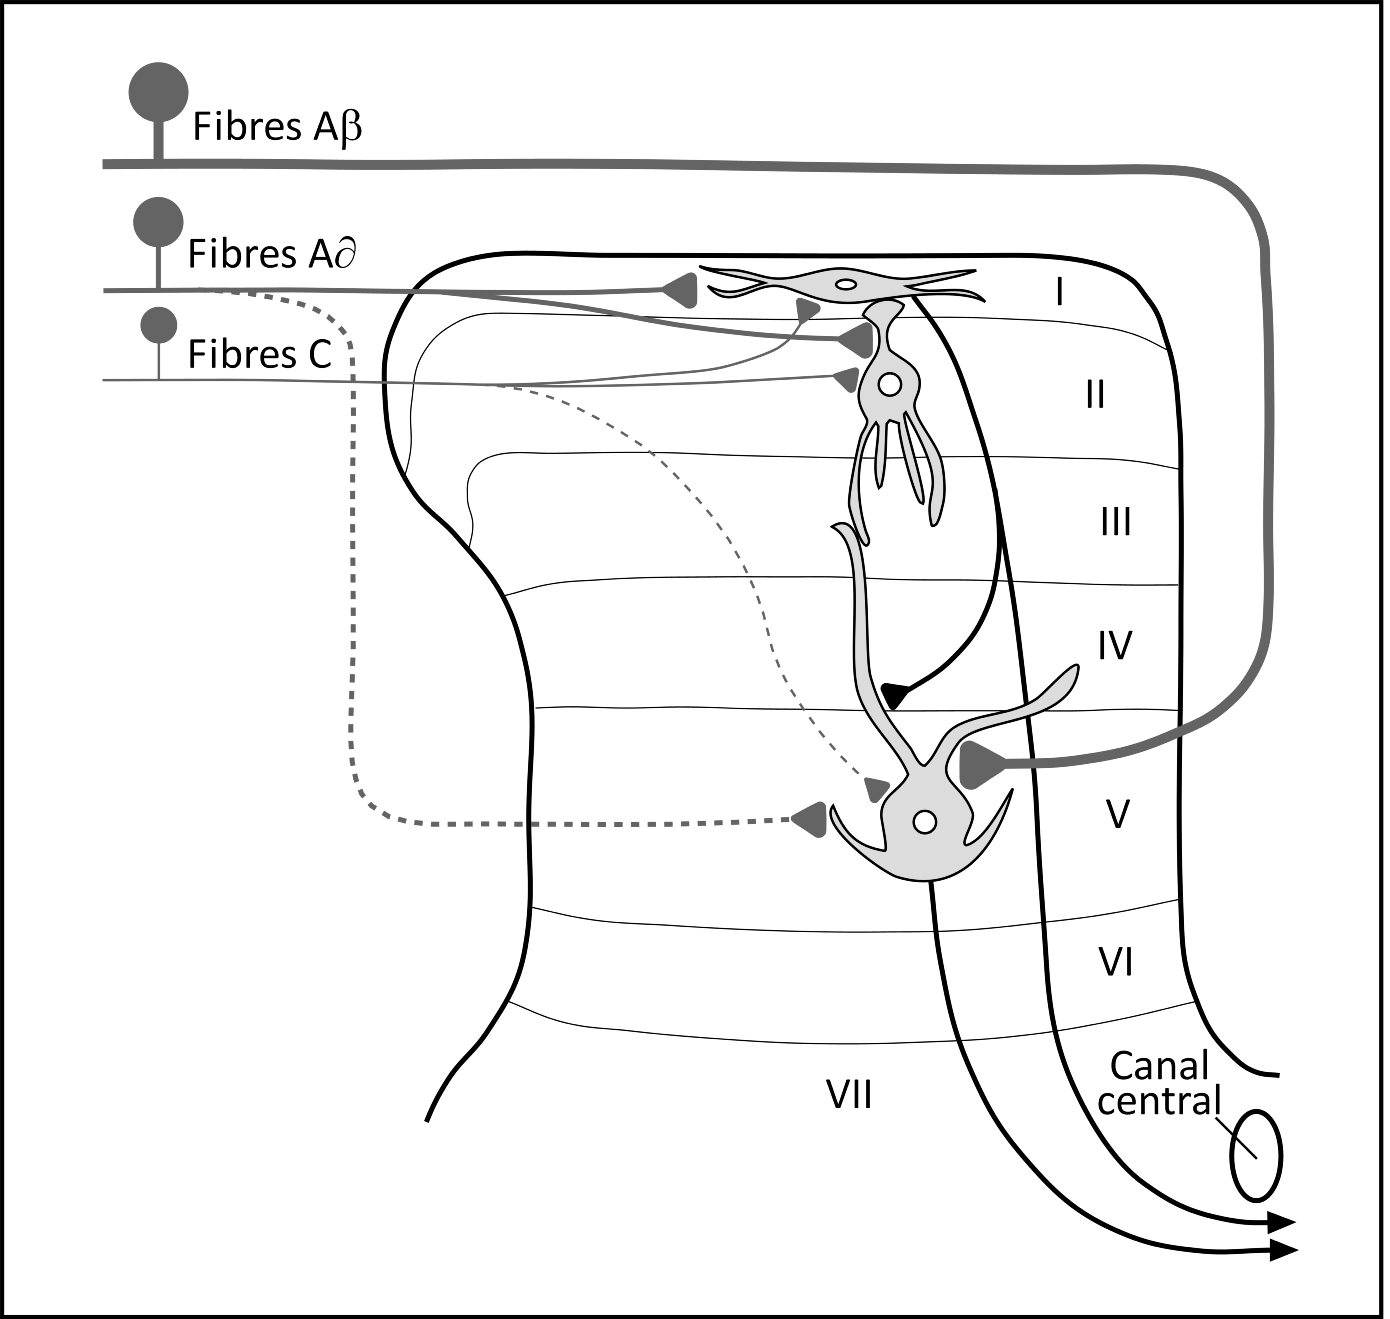
\includegraphics{Figure1.jpg} 
\end{center}

\caption{\textbf{Innervation nociceptive de la corne dorsale de la moelle épinière}}

{\protect\parbox[t]{18cm}{
\begin{small}Les neurones des couches I et II reçoivent une projection massive de fibres nociceptives A$\delta$ et C. Les neurones de la couche V reçoivent seulement une projection modeste des fibres A$\delta$ et C; en revanche, ils reçoivent une projection dense des neurones des couches I et II. Ils reçoivent aussi une importante projection des fibres tactiles A$\beta$.\\
I – VI : couches I à VI de la corne dorsale de la moelle épinière; VII : couche VII de la région intermédiaire de la substance grise de la moelle épinière. (Figure tirée de Bernard et Villanueva 2009) \end{small}}}

\label{Figure 1}

\end{figure}


En plus de ces deux régions superficielle et profonde, il faut noter que des neurones activés par des stimuli nociceptifs cutanés et viscéraux ont été enregistrés encore plus profondément au niveau des couches VII et X. Ils ont des caractéristiques complexes et souvent des champs récepteurs étendus.

\bigskip 

Cette distinction couches superficielles/couches profondes quant à la nature de leurs afférences se retrouve aussi au niveau de leurs efférences. Ainsi ces différentes régions de la moelle épinière donnent naissance à des contingents de fibres projetant sur des structures supraspinales clairement identifiées.

\section{Les voies ascendantes de la nociception}

Les axones des neurones nociceptifs secondaires effectuent une décussation à un niveau proche du segment spinal d'origine. Ils forment ensuite une colonne de fibres ascendantes localisée principalement dans le quadrant ventrolatéral/latéral contralatéral de la substance blanche. Toutefois, un contingent appréciable de neurones de second ordre (surtout ceux des couches profondes) ne croise pas et projette directement sur des structures supraspinales ipsilatérales. Il est possible de distinguer plusieurs voies nociceptives en fonction de la région de la corne dorsale (superficielle ou profonde) d’où elles sont issues (Bernard \& Villanueva 2009).

A partir des couches superficielles, on peut identifier des projections :

\begin{itemize}
\item dans l’aire parabrachiale latérale (PBl), 
\item dans la partie ventrolatérale de la substance grise périaqueducale (PAG), et 
\item dans le thalamus latéral (noyau ventropostérolatéral) (voir Figure \ref{Figure 2} - page \pageref{Figure 2}).
\end{itemize}

A partir des couches profondes on trouve deux voies vers le thalamus médian :
 
\begin{itemize}
\item une projection directe sur les noyaux thalamiques intralaminaires, et 
\item une voie indirecte qui passe d’abord dans la partie interne latérale du noyau parabrachial (PBil) et le sous-noyau réticulé dorsal (SRD) (voir Figure \ref{Figure 3} - page \pageref{Figure 3}).
\end{itemize}


Notons que les couches profondes nociceptives projettent aussi sur le noyau réticulaire latéral (LRt - qui projette massivement sur le cervelet), sur le noyau réticulaire gigantocellulaire (Gi) et dans une moindre mesure sur l'hypothalamus latéral et le striatum.

\subsection{Projections des neurones de la couche I}

\subsubsection{Couche I –Aire parabrachiale latérale}

Cette voie concerne un peu plus de la moitié des neurones de la couche I (voir Figure \ref{Figure 2} - page \pageref{Figure 2}). Compte tenu des structures qu’elle contacte, elle joue probablement un rôle très important dans les composantes émotionnelles et neurovégétatives de la nociception. La majorité des projections au PBl est directe (Cechetto et al. 1985; Bernard et al. 1995) mais une minorité fait d’abord étape au niveau du noyau du tractus solitaire (NTS) (Raboisson et al. 1996). Une très grande proportion des neurones du PBl répondent spécifiquement à des stimuli nociceptifs et en codent l'intensité dans la gamme nociceptive (Bernard \& Besson 1990; Bernard et al. 1994; Bester et al. 1995). D’une part, ces neurones nociceptifs du PBl projettent en majorité sur le noyau central de l’amygdale (voir Figure \ref{Figure 2} - page \pageref{Figure 2}) et celui du lit de la strie terminale, deux régions impliquées dans les réactions de peur, d’anxiété et de stress. D’autre part ils projettent sur le noyau ventromédian de l’hypothalamus (VMH) (Bester et al. 1997), qui contrôle à la fois les comportements de défense et d'agressivité (voir « \ref{Nociception,réaction de défense,effets cardiovasculaires} Nociception et réaction de défense : effets cardiovasculaires » - page \pageref{Nociception,réaction de défense,effets cardiovasculaires}), et le métabolisme énergétique. Il faut noter toutefois qu’une partie des efférences du PBl projette aussi vers la PAG et la partie ventrolatérale du bulbe.

\subsubsection{Couche I – Substance grise périaqueducale}

Environ un quart des neurones de la couche I sont concernés par cette voie (voir Figure \ref{Figure 2} - page \pageref{Figure 2}). Elle semble être impliquée dans certaines des réactions de défense induites par la nociception. En effet, lorsque l’on stimule les colonnes ventrolatérales et latérales de la PAG, qui reçoivent des projections des neurones de la couche I, on peut déclencher des réactions cardiovasculaires et défensives spécifiques. Celles-ci comprennent des modifications de la pression artérielle et de la motricité, des comportements d’évitement, une vocalisation et des effets antinociceptifs indépendants des systèmes opioïdergiques mais qui semblent médiés par la région rostroventrale du bulbe (Depaulis \& Bandler 1991).

\subsubsection{Couche I – Thalamus}

Cette voie ne concerne qu’une faible proportion de neurones de la couche I (voir Figure \ref{Figure 2} - page \pageref{Figure 2}). Ils projettent sur le complexe postérieur (Po), la partie triangulaire du complexe postérieur (PoT) et les noyaux ventraux postérolatéral et médian (VPL et VPM) du thalamus. La projection sur le VPL correspond aux informations d'origine spinale et celle sur le VPM aux informations issues du territoire céphalique (Craig 1991; Vos et al. 2000)
\footnote{Il est important de noter que ces noyaux thalamiques sont également les sites de projection de la voie des colonnes dorsales qui véhiculent les informations tactiles.}. 
Par ses projections de sortie vers les aires corticales somatosensorielles S1 et S2, cette voie est probablement responsable de la composante sensori-discriminative de la douleur. Pour sa part, le contingent de projection « couche I – PoT - cortex insulaire » aurait un rôle plus spécifique dans la composante affectivo-émotionnelle de la douleur.

\begin{figure}[p]

\begin{center}
 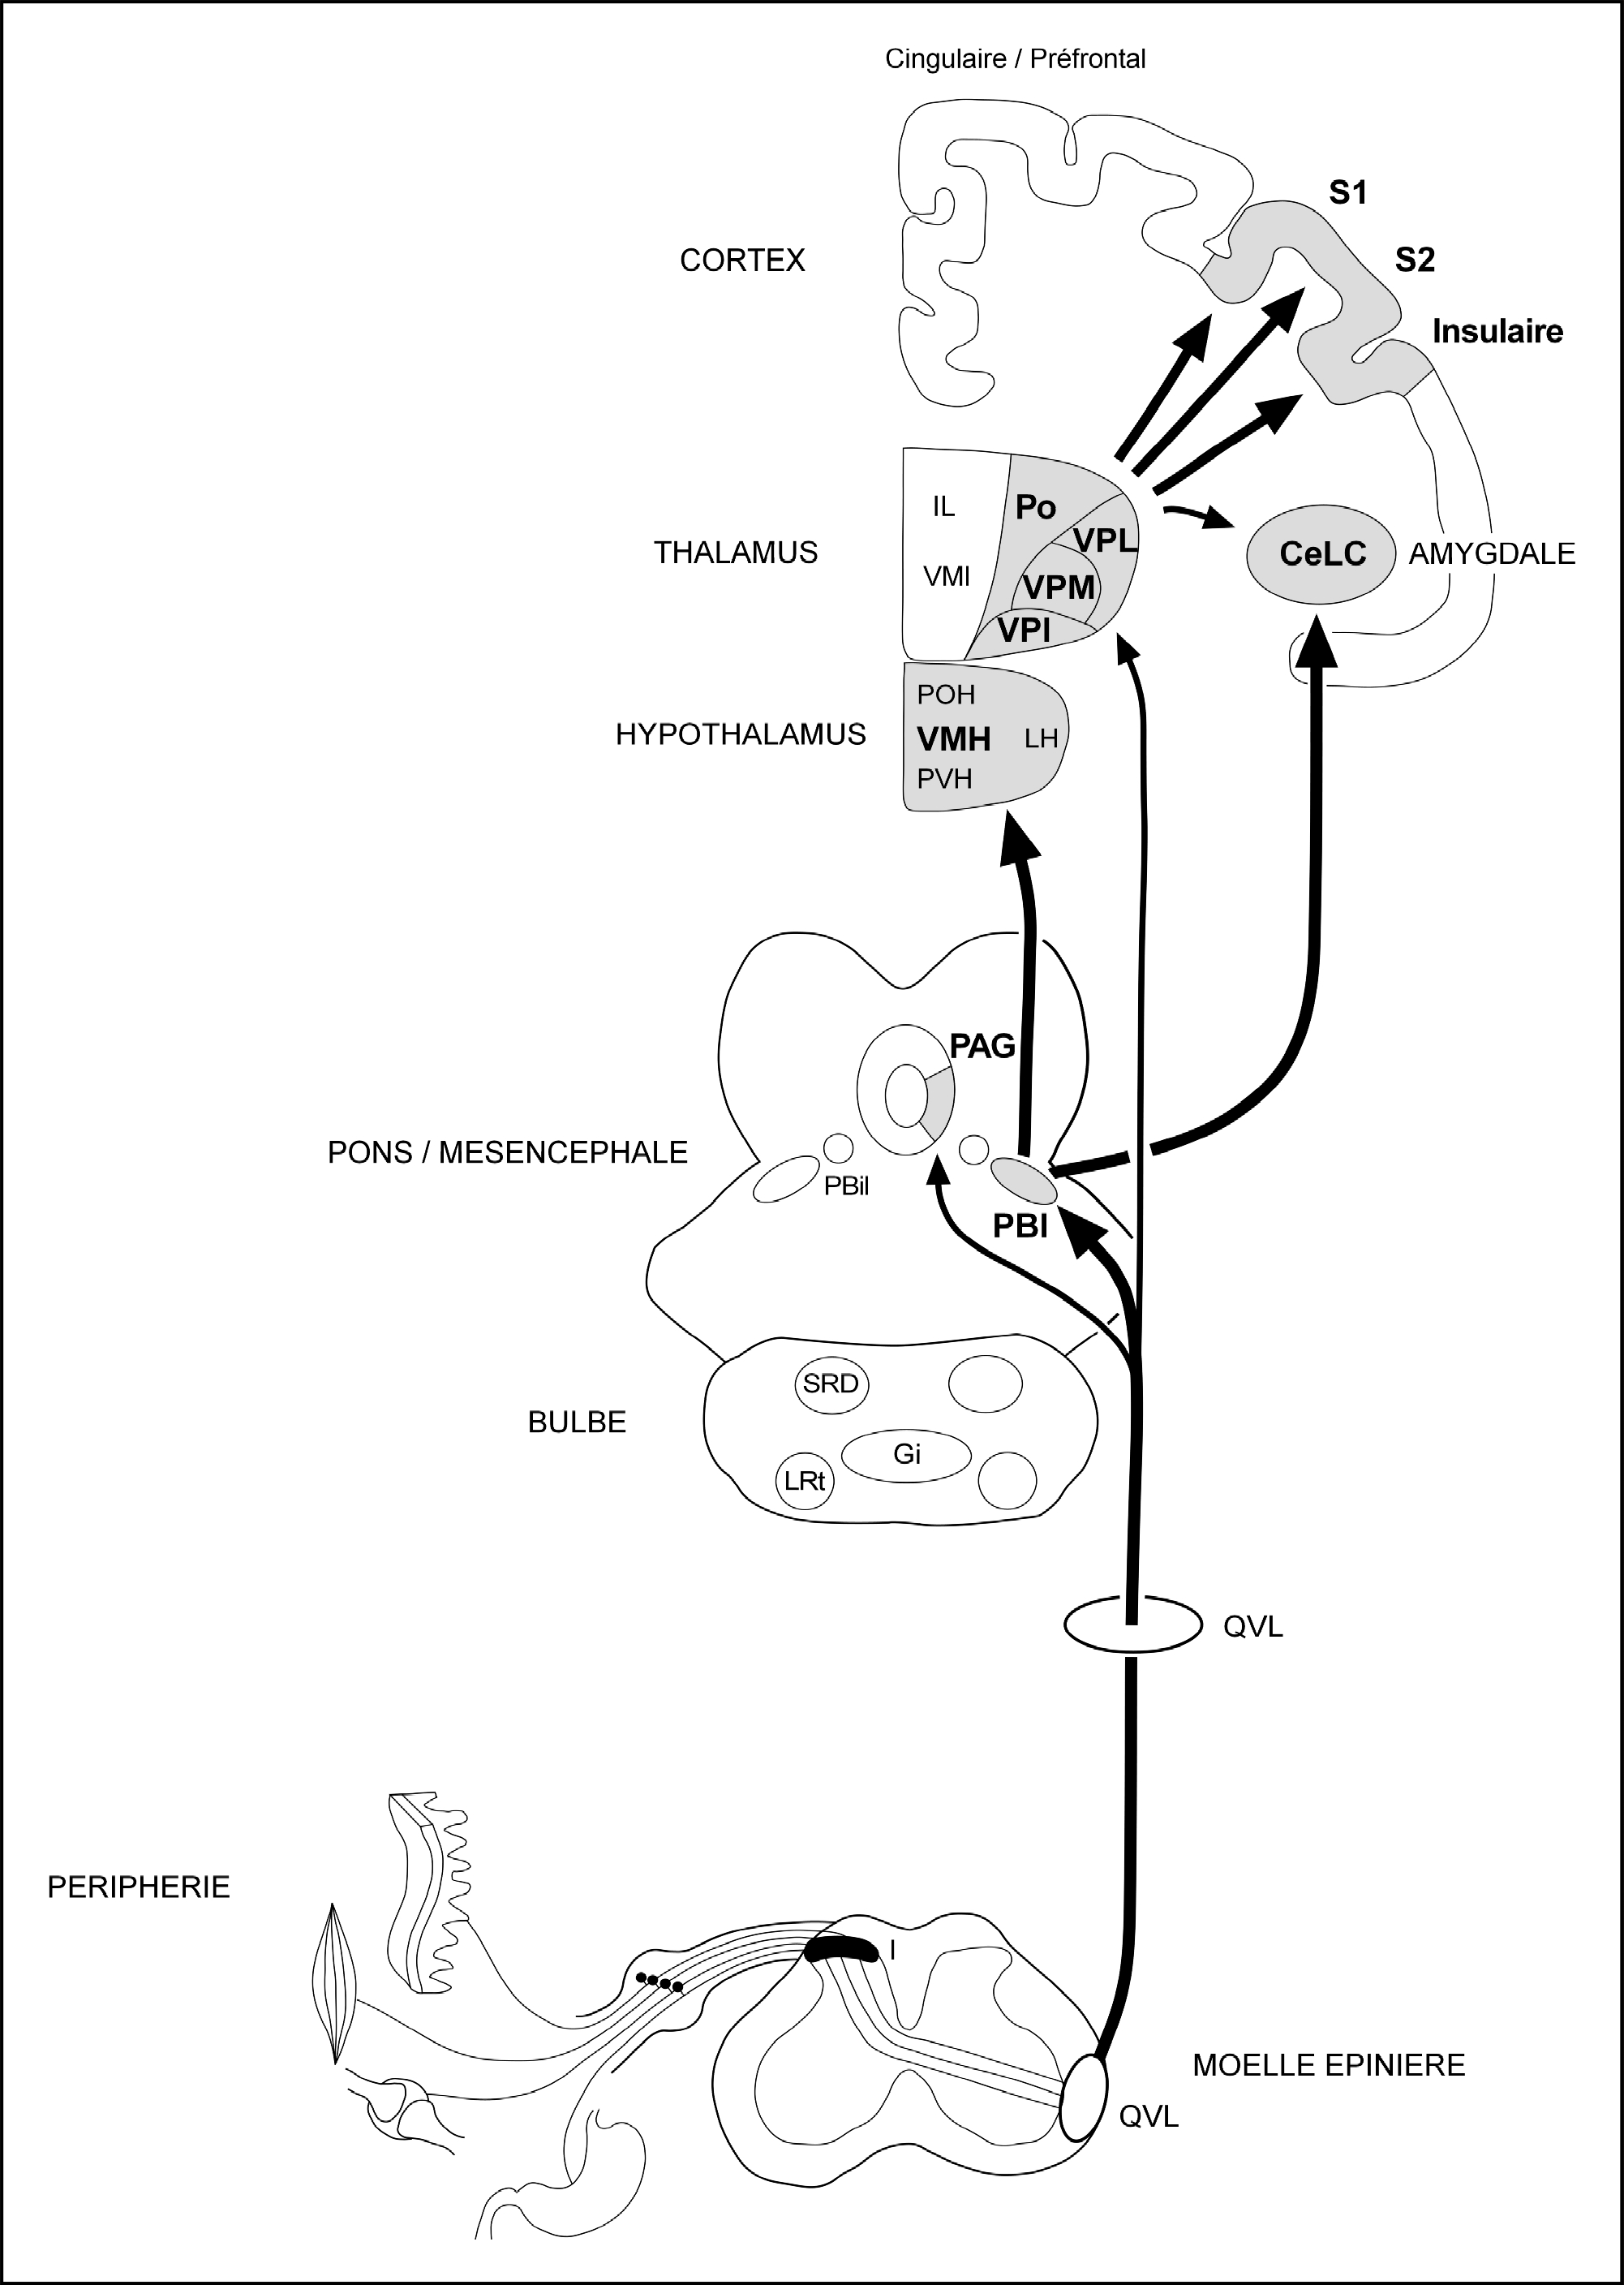
\includegraphics[scale=0.75]{Figure2.jpg} 
\end{center}

\caption{\textbf{Les voies nociceptives issues de la couche I}}

{\protect\parbox[t]{18cm}{
\begin{small}Les axones des neurones de la couche I de la corne dorsale de la moelle épinière croisent la ligne médiane au niveau de leur origine segmentaire. Ils se regroupent dans la partie dorsale du quadrant ventrolatéral de la moelle (QVL) pour monter vers le bulbe. Ces neurones projettent essentiellement sur le noyau parabrachial latéral (PBl), la substance grise périaqueducale (PAG) et le thalamus latéral. Le PB projette à son tour sur l'amygdale et l'hypothalamus. Le thalamus latéral projette sur les aires corticales somatosensorielles, primaire (S1), secondaire (S2) et insulaire ainsi que sur l'amygdale. L'épaisseur des traits représente la densité et l'importance des faisceaux véhiculant les messages nociceptifs.\\
CeLC : noyau central, partie latérale capsulaire (amygdale) ; Gi : noyau réticulaire gigantocellulaire ; IL : noyau intralaminaire (thalamus médian) ; LH : région latérale (hypothalamus) ; I : couche I de la corne dorsale ; LRt : noyau réticulaire latéral ; Po : complexe postérieur (thalamus latéral) ; POH : région préoptique (hypothalamus) ; PVH : noyau paraventriculaire (hypothalamus) ; SRD : sous-noyau réticulaire dorsal du bulbe ; VMH : noyau ventromédian (hypothalamus) ; VMl : noyau ventromédial latéral (thalamus médian) ; VPI : noyau ventropostéroinférieur (thalamus latéral) ; VPL : noyau ventropostérolatéral (thalamus latéral) ; VPM : noyau ventropostéromédian (thalamus latéral). (Figure modifiée à partir de Bernard et Villanueva 2009) \end{small}}}

\label{Figure 2}

\end{figure}

\clearpage

\subsection{Projections des neurones de la couche V}

\subsubsection{Couche V - Noyau réticulé latéral}

Le LRt est un noyau réticulaire étroitement lié au cervelet. Il pourrait être directement impliqué dans les réactions motrices en réponse à des messages nociceptifs et proprioceptifs en provenance des neurones de la couche V (Raboisson et al. 1996). 

\subsubsection{Couche V – Noyau réticulé gigantocellulaire}

Il existe une projection des neurones de la couche V sur la portion caudale du Gi (voir Figure \ref{Figure 3} - page \pageref{Figure 3}). Celui-ci projette à son tour vers les noyaux intralaminaires du thalamus, le locus cœruleus, le noyau du tractus solitaire, les noyaux moteurs du bulbe et la corne ventrale de la moelle épinière (Martin et al. 1985; Ohtake 1992; Luppi et al. 1995). De nombreux neurones du Gi répondent à des stimuli nociceptifs, mais peuvent aussi être activés par d'autres modalités sensorielles (Casey 1971; Bowsher 1976). Il semblerait que le Gi joue un rôle notable dans les manifestations motrices et végétatives, ainsi que dans l'éveil et l'état d'alerte déclenchés par toute stimulation nociceptive.

\subsubsection{Couche V – Sous-noyau réticulé dorsal}

Le SRD reçoit des afférences provenant de la couche V de tous les segments de la moelle épinière (voir Figure \ref{Figure 3} - page \pageref{Figure 3}). Les neurones du SRD ne répondent pas à des stimuli visuels, auditifs, ou proprioceptifs, mais sont fortement activés depuis n’importe quel territoire corporel par la stimulation des fibres A$\delta$ et C. Ils codent l’intensité d’une stimulation cutanée ou viscérale dans une gamme nociceptive (Villanueva et al. 1988; Villanueva et al. 1989; Villanueva et al. 1990).

Le SRD projette sur l’ensemble des segments spinaux et participe ainsi à une boucle spino-bulbo-spinale (Bernard et al. 1990; Villanueva et al. 1991) jouant un rôle important dans certaines modulations de la nociception (Bouhassira et al. 1992b) (voir « \ref{Modulations hétérosegmentaires} Modulations hétérosegmentaires de la nociception » - page \pageref{Modulations hétérosegmentaires} »). Par ailleurs, le SRD envoie aussi une projection massive sur deux structures du thalamus médian (voir Figure \ref{Figure 3} - page \pageref{Figure 3}) : d’une part la partie latérale du noyau ventromédian (VMl) et d’autre part, mais à un degré moindre, le noyau parafasciculaire (Pf) (Villanueva et al. 1998). Le VMl véhicule les influx nociceptifs vers la couche superficielle du cortex préfrontal et frontal dorsolatéral, alors que le Pf projette vers le cortex pré-moteur antérieur, le striatum dorsolatéral et le subthalamus latéral. Ainsi, le circuit « couche V – SRD – VMl/Pf – cortex frontal » induirait une excitation corticale diffuse subliminaire, et aurait ainsi un rôle d'éveil et d'amplification des composantes sensorimotrices (via le VMl) et émotionnelles (via le Pf) de la nociception (Villanueva et al. 1998).

\subsubsection{Couche V – Aire parabrachiale interne latérale}

Le PBil reçoit une projection dense de la couche V de la moelle épinière, en particulier de sa région réticulaire (Bernard et al. 1995). La plupart des neurones du PBil répondent à des stimuli nociceptifs avec une très longue post-décharge, et sont sensibles à la morphine (Bester et al. 1999). Le PBil projette principalement sur le noyau paracentral du thalamus (voir Figure \ref{Figure 3} - page \pageref{Figure 3}) et dans une moindre mesure, sur le noyau parafasciculaire (Pf) (Fulwiler \& Saper 1984; Bester et al. 1999). Ces deux noyaux envoient à leur tour des projections diffuses sur le cortex préfrontal, le cortex cingulaire et les compartiments correspondants du striatum (noyau caudé et putamen) (Berendse \& Groenewegen 1991). Ce circuit « couche V – PBil – PC/Pf – cortex préfrontal » pourrait participer à la mise en alerte de l'individu au cours du processus nociceptif.

\begin{figure}[p]

\begin{center}
 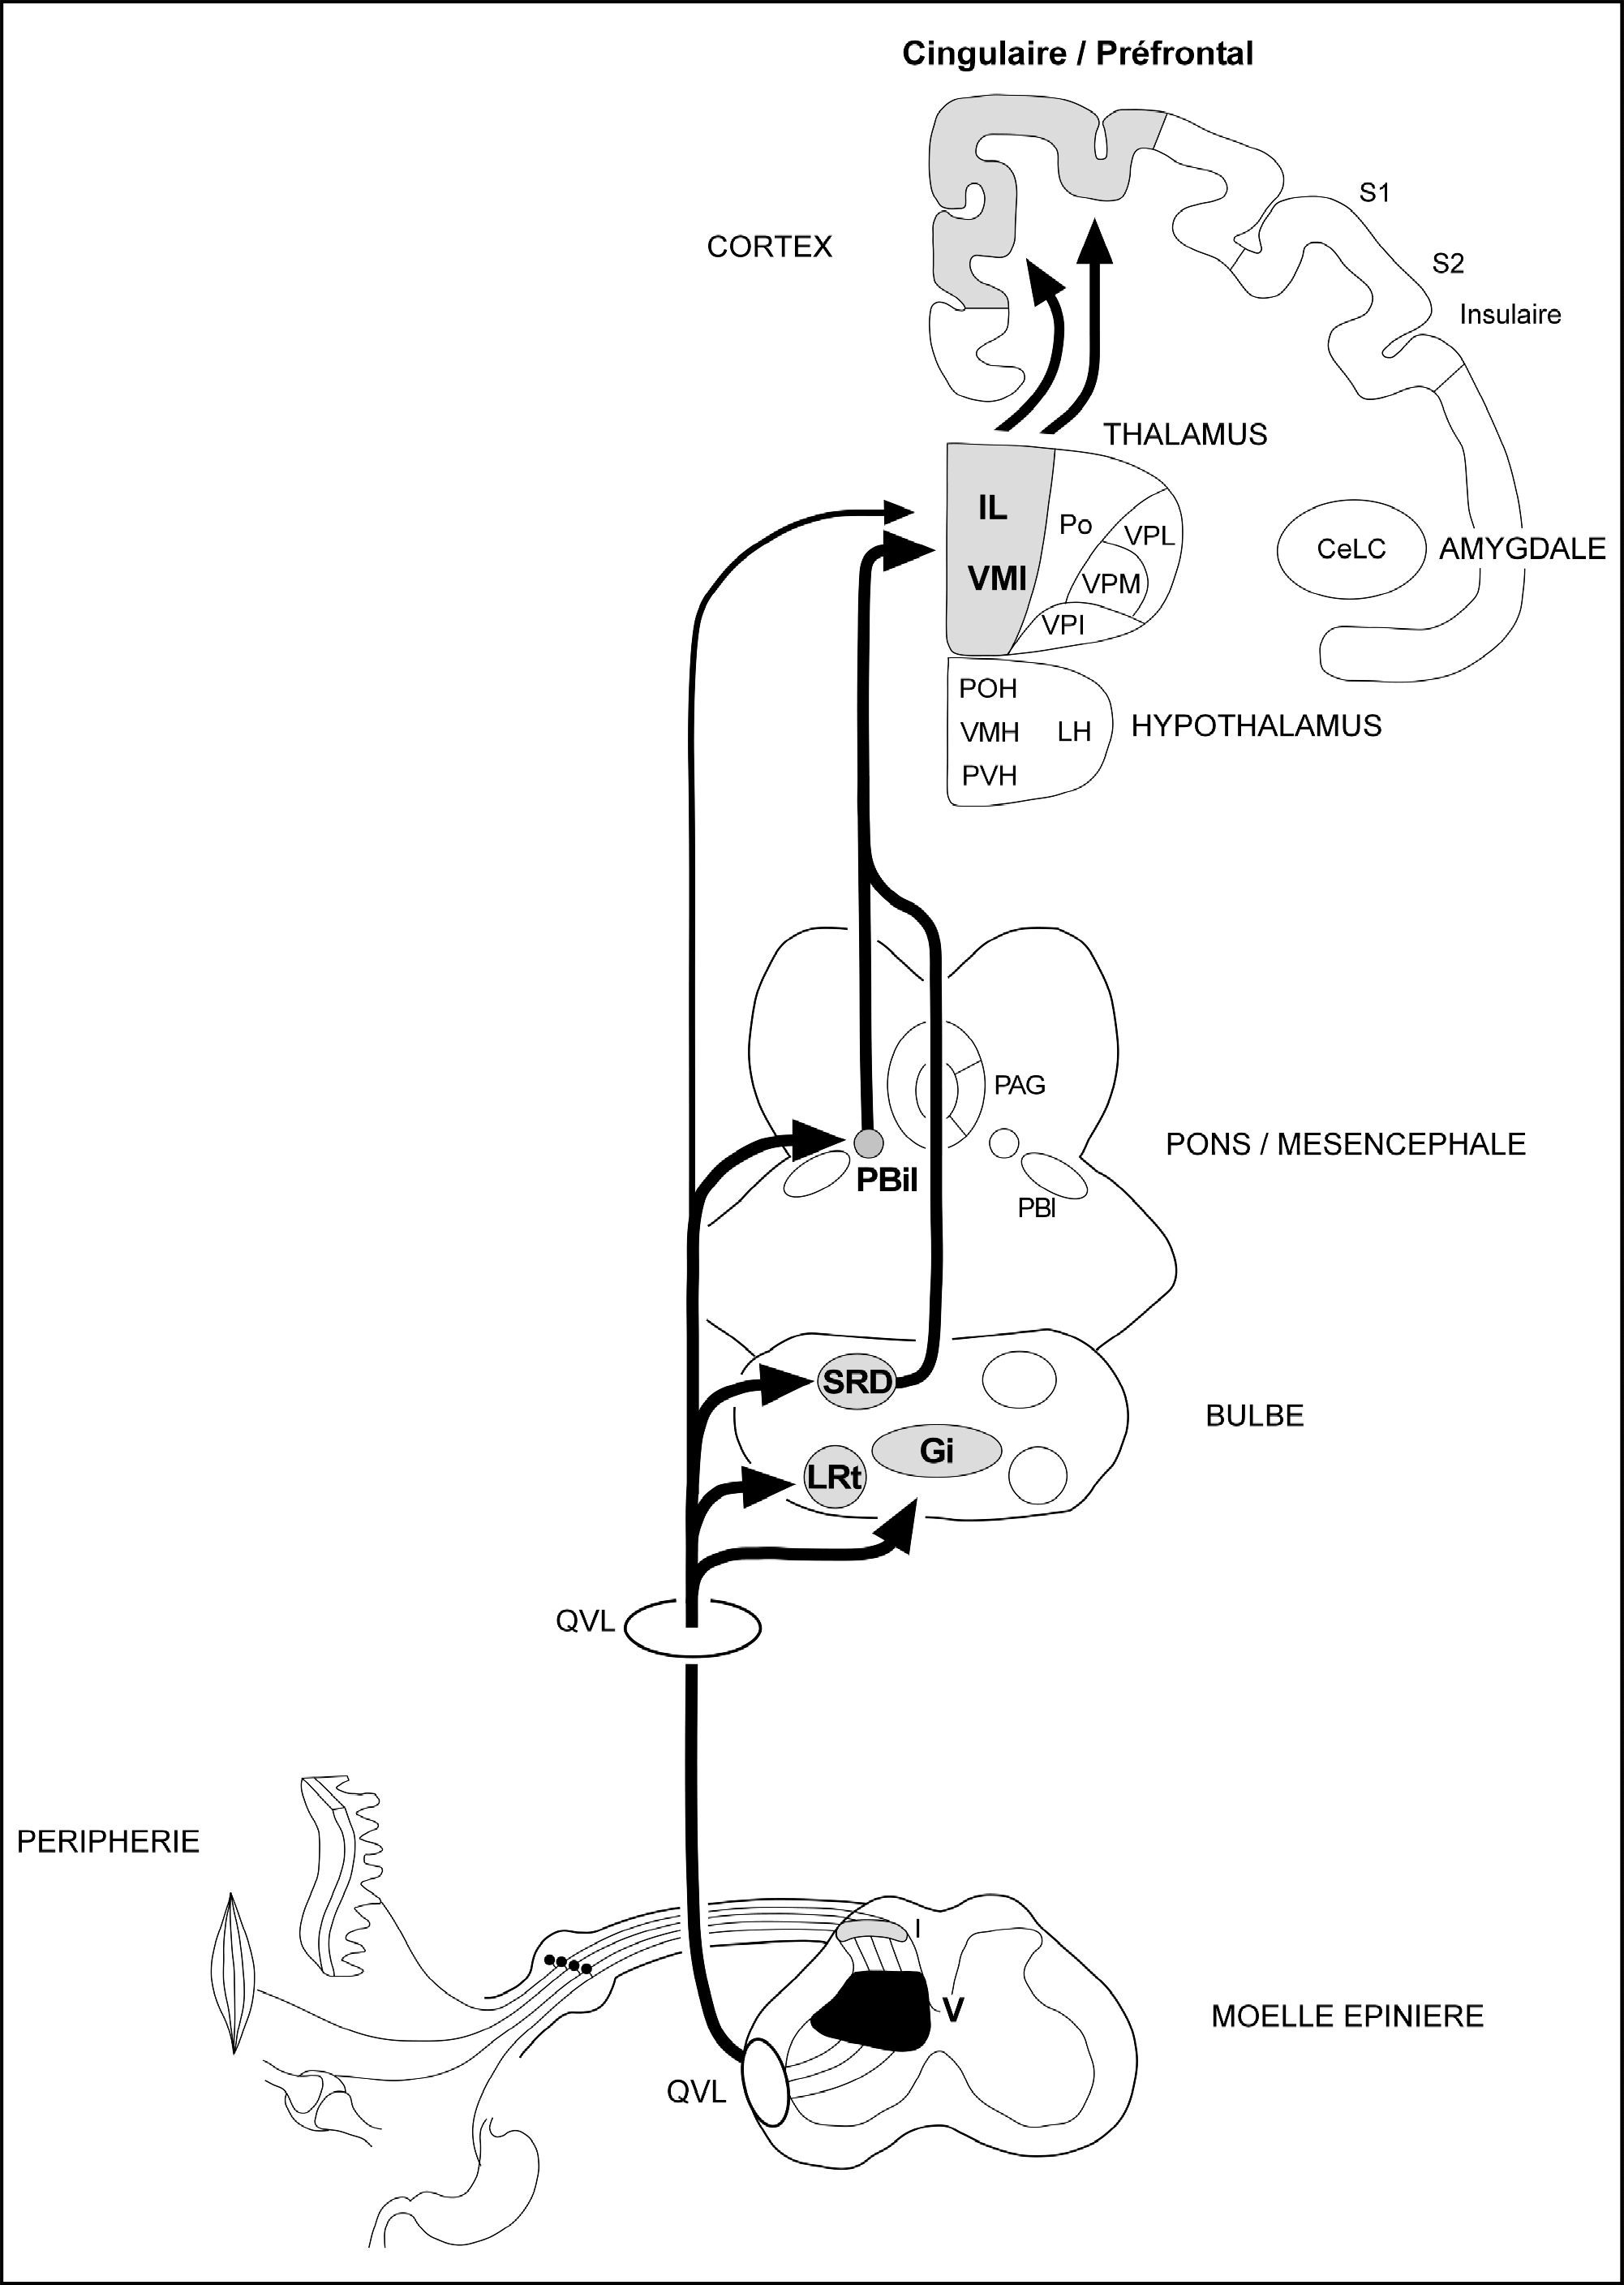
\includegraphics[scale=0.85]{Figure3.jpg} 
\end{center}

\caption{\textbf{Les voies nociceptives issues de la couche V}}

{\protect\parbox[t]{18cm}{
\begin{small}Les axones des neurones de la couche V de la corne dorsale de la moelle restent en majorité homolatéraux au niveau de leur origine segmentaire. Ils se regroupent dans la partie dorsale du quadrant ventrolatéral de la moelle (QVL) pour monter vers le bulbe. Ces neurones projettent essentiellement sur les noyaux réticulaires latéral (LRt), gigantocellulaire (Gi) et dorsal (SRD) ainsi que sur le sous-noyau parabrachial latéral interne (PBil) et sur le thalamus médian (noyaux intralaminaires [IL] et ventromédial latéral [VMl]). Le thalamus médian projette à son tour sur les aires corticales cingulaires et préfrontales.\\ L'épaisseur des traits représente la densité et l'importance des faisceaux véhiculant les messages nociceptifs. V : couche V de la corne dorsale ; autres abréviations: voir Figure \ref{Figure 2} - page \pageref{Figure 2}. (Figure modifiée à partir de Bernard et Villanueva 2009) \end{small}}}

\label{Figure 3}

\end{figure}

\clearpage

\section{Structures cérébrales et nociception}

Pour résumer et compléter les données rapportées plus haut sur les cibles supraspinales des voies de la nociception, il convient de distinguer deux grandes catégories de structures impliquées dans le traitement de l’information nociceptive au niveau supraspinal

Tout d’abord, les structures « profondes » sont impliquées dans des réactions motrices, aversives automatiques et non directement conscientes à un stimulus nociceptif. Ces structures incluent l'amygdale, l'hypothalamus, le globus pallidus, la PAG, le PB, la formation réticulée et le cervelet. La mise en jeu de ces structures conduirait des réponses coordonnées avec, en particulier, un éveil et une attention généralisée, des réactions émotionnelles (aversion, évitement), des comportements défensifs, actifs ou passifs, une adaptation des paramètres végétatifs et des réactions motrices réflexes.

Ensuite, les zones corticales en relation directe avec le thalamus postérieur jouent un rôle clé dans la perception consciente de la nociception. On distingue le cortex somatosensoriel SI, qui traite les messages spinaux tactiles aussi bien que nociceptifs, le cortex SII, qui intègre les messages dont l'intensité est potentiellement dangereuse, et le cortex insulaire, qui pourrait générer la sensation d'algosité (c'est-à-dire son caractère désagréable) (Fields 1999). Ces informations sont transmises aux cortex cingulaire et préfrontal, qui complètent l’intégration en termes cognitifs et émotionnels. Dans ce contexte, le thalamus latéral jouerait surtout un rôle dans la transmission des messages tactiles et nociceptifs, le thalamus médian surtout un rôle d'alerte et d'amplification.

L’analyse de diverses lésions cérébrales en neurologie a permis d’établir le rôle fonctionnel spécifique de certaines de ces zones, notamment chez des patients présentant des « doubles dissociations » des composantes sensori-discriminatives et affectivo-émotionnelles de la douleur.

\begin{description}
\item Ainsi des lésions touchant les aires corticales insulaires se caractérisent par un tableau clinique de type « asymbolie à la douleur » (Berthier et al. 1988). Chez les patients concernés, la composante affectivo-émotionnelle de la douleur est atteinte mais pas la composante sensori-discriminative. On note chez eux une absence totale ou une diminution radicale des réactions motrices et affectives à des stimulations nociceptives, mais leur capacité de discrimination de tels stimuli demeure intacte. Ces patients présentent en réalité une hyporéactivité émotionnelle à la douleur (Berthier et al. 1988; Danziger 2006). Un autre type de lésion aux conséquences bien différentes est la lobotomie préfrontale. Dans ce cas, la douleur n'a pas disparu et son intensité n'est pas modifiée, mais elle laisse le patient indifférent (Berthier et al. 1988; Danziger 2006).

\item \`A l’inverse, une lésion des cortex somatosensoriels SI et SII entraîne un tableau clinique opposé. Le patient ressent une sensation franchement désagréable, qu’il souhaite éviter lorsque les stimuli thermiques deviennent nociceptifs, mais il s’avère incapable de décrire la qualité, la localisation et l’intensité de ces stimuli (Ploner et al. 1999). 
\end{description}


Toutefois, ces résultats doivent être nuancés par les apports de l’imagerie fonctionnelle. Les investigations en IRM fonctionnelle en particulier ont montré que la douleur active en fait toute une « matrice » de structures et que, malgré une spécialisation fonctionnelle relative de certaines d’entres elles, le traitement parallèle des composantes sensorielles et émotionnelles n’est pas aussi net que le laissaient penser les premières études (Price 2000; Apkarian et al. 2005; Price et al. 2006).

\cleardoublepage

\chapter{Systèmes de contrôles de la nociception}

Selon les situations, des systèmes de modulation positive ou négative peuvent intervenir pour modifier le seuil de détection d’un stimulus nociceptif. Ainsi, lors d’une agression par un prédateur, il est préférable pour la survie de l’individu de « mettre en veille » la transmission de l’information nociceptive afin de permettre une réponse appropriée (fuite, attaque) : se mettent alors en action des systèmes inhibiteurs de la nociception. A contrario, une fois à l’abri, il peut être important pour l’organisme de ménager un membre blessé ; des systèmes facilitant la transmission de l’information nociceptive pouvant alors être mis en jeu.

Un site privilégié de modulation est la corne dorsale de la moelle épinière, site du premier relais des messages nociceptifs. À ce niveau, existent trois types de modulations que l’on peut classer en fonction de leur origine : 

\begin{enumerate}
\item les \textit{inputs} modulateurs et les \textit{inputs} nociceptifs sont issus d’un même territoire corporel et convergent vers le même segment de moelle : on parle de modulation segmentaire ; 
\item une stimulation nociceptive appliquée à une partie du corps vient moduler l’information nociceptive issue d’un autre territoire corporel : on parle de modulation hétérosegmentaire ; 
\item la modulation met en jeu des structures supraspinales : on parle alors de contrôles descendants.
\end{enumerate}

Dans les paragraphes suivants, je décrirai les deux derniers plus en détail.

\section{Modulations hétérosegmentaires de la nociception}
\label{Modulations hétérosegmentaires} 

Ce type de modulation, qui concerne les neurones WDR, est plus connu sous le nom de « contrôle inhibiteur diffu induit par des stimulations nociceptives » (CIDN).

Ainsi, les réponses de ces neurones à tout type de stimulation peuvent être inhibées par une stimulation clairement nociceptive appliquée en dehors de leur champ récepteur, y compris au niveau viscéral. Ce type d’inhibition a été mis en évidence chez le rat (Le Bars et al. 1979b; 1979a), le chat (Morton et al. 1987) et le singe (Gerhart et al. 1981). Un phénomène similaire a été décrit chez l’être humain chez qui un stimulus douloureux conditionnant hétérotopique déprime le réflexe RIII du biceps fémoral déclenché par stimulation du nerf sural (Willer et al. 1984). Ce type d’inhibition concerne le corps entier et ne présente pas d’organisation somatotopique particulière. Tous les neurones WDR semblent concernés y compris ceux qui projettent au thalamus (Dickenson \& Le Bars 1983). Les premières études sur les CIDN montraient que les neurones de la couche I ne semblent pas être affectés par ces contrôles (Le Bars et al. 1979b; Dickenson et al. 1980; Villanueva et al. 1984b; 1984a), toutefois des études plus récentes sont venues contredire ces résultats (Morgan et al. 1994; Meng et al. 1997; Bester et al. 2000). Les fibres véhiculant cette inhibition au niveau périphérique ont des vitesses de conduction de 0,5 à 8 m/s suggérant l’implication surtout des fibres C et un peu moins des fibres A$\delta$ (Bouhassira et al. 1987). Les CIDN mettent en jeu une boucle spino-bulbo-spinale, puisqu’ils sont absents chez l’animal dont la moelle épinière a été sectionnée (Le Bars et al. 1979b). Les composantes ascendante et descendante sont véhiculées respectivement dans les quadrants ventro- et dorso-latéral (Villanueva et al. 1986a; Villanueva et al. 1986b). Aucune des structures classiquement mises en jeu dans les contrôles descendants (voir ci-dessous) n’est impliquée dans cette boucle (Bouhassira et al. 1990; 1992a; 1993a; Bouhassira et al. 1993b). Les CIDN semblent plutôt recruter les neurones du sous-noyau réticulaire dorsal (Bouhassira et al. 1992b).

Comme nous l’avons vu, les neurones WDR répondent à des stimulations nociceptives et non nociceptives. Ainsi, dans les conditions physiologiques, ces neurones sont en permanence soumis à des \textit{inputs} sensoriels, à l’origine d’une activité électrophysiologique constituant un véritable « bruit de fond ». Lors d’une stimulation nociceptive, la mise en jeu des CIDN induit une augmentation du rapport « signal nociceptif/bruit de fond », permettant ainsi à l’organisme de mieux discriminer la présence d’un stimulus nocif. 

\section{L’axe « PAG-RVM-corne dorsale »}

Très tôt, Charles Sherrington (1896) a montré que des animaux décérébrés présentaient une rigidité motrice, et qu’il existait donc des influences descendantes inhibitrices à même de moduler des circuits spinaux (Sherrington 1906). En 1969, David Reynolds a montré que la stimulation électrique continue d’une région proche de la partie dorsolatérale de la substance grise périaqueducale (PAG) n’affectait pas le comportement moteur du rat, mais induisait une analgésie suffisante pour permettre une laparotomie sans qu’une autre forme d’anesthésie soit nécessaire (Reynolds 1969). Cette expérience princeps a rapidement amené à toute une série d’études pour mettre en évidence les circuits supra-spinaux impliqués dans ce contrôle inhibiteur descendant, relativement spécifique de la douleur.

Les effets analgésiques de stimulations ont été observés chez plusieurs espèces (Oliveras et al. 1974; Hayes et al. 1979), y compris chez l’être humain (Hosobuchi et al. 1977; Richardson \& Akil 1977b; 1977a; Young et al. 1985). On sait aujourd’hui que ce type d’analgésie par stimulation électrique profonde peut être obtenu à partir de plusieurs structures comme : la PAG (Reynolds 1969; Mayer et al. 1971), la région rostroventromédiane du bulbe (RVM) (Oliveras et al. 1975), plusieurs noyaux hypothalamiques, le noyau parabrachial (PB) (DeSalles et al. 1985), le noyau du tractus solitaire (NTS) (Lewis et al. 1987; Morgan et al. 1989b). Une analgésie peut également être induite par des stimulations corticales, notamment des cortex insulaire et orbital ventrolatéral (Zhang et al. 1997; Jasmin et al. 2003).

Il est aujourd’hui clairement établi que ces modulations impliquent de très nombreux neurotransmetteurs, neuromodulateurs et neuropeptides, même si les opioïdes endogènes et les monoamines (sérotonine, dopamine, noradrénaline) (Akil \& Liebeskind 1975) sont au premier plan dans la genèse dans ces effets.

\bigskip 

Le circuit impliqué dans les contrôles descendants qui est le plus étudié, et probablement le mieux caractérisé, est l’axe « PAG-RVM-corne dorsale ». Pour certains, il serait la « voie de sortie » de la grande majorité des contrôles descendants. 

Etant donné l’existence de relations anatomiques étroites entre la PAG et la RVM d’une part, et les projections denses de la RVM vers la corne dorsale de la moelle d’autre part (voir « \ref{Anatomie RVM} Anatomie de la région rostroventromédiane du bulbe » – page \pageref{Anatomie RVM}), ces structures clé dans l’analgésie par stimulation électrique ont très tôt été proposées comme faisant partie d’un système spinopète modulateur de la nociception et partiellement impliqué dans les effets analgésiques de la morphine (Basbaum \& Fields 1978; Fields \& Basbaum 1978).

La première hypothèse supposait une modulation de type \textit{top-down} avec 3 niveaux (Basbaum \& Fields 1978; Fields \& Basbaum 1978). Le point de départ se situant dans la PAG. La RVM joue le rôle de relais, et projette via le quadrant dorsolatéral de la moelle sur la corne dorsale (principalement dans les couches superficielles), où se fait la modulation finale des \textit{inputs} nociceptifs (Basbaum \& Fields 1978; Basbaum \& Fields 1984; Fields et al. 1991). Il apparait maintenant clairement que ce circuit est lui-même influencé via la PAG par d’autres structures situées en amont comme les cortex cingulaire antérieur et insulaire, l’amygdale, ou certaines structures hypothalamiques (Fields 2004; McGaraughty et al. 2004). 

Considéré à l’origine comme strictement inhibiteur, cet axe est, depuis le courant des années 90, de plus en plus vu comme un système pouvant se révéler inhibiteur ou excitateur selon les circonstances (Urban \& Gebhart 1999; Porreca et al. 2002; Fields 2004). Par ailleurs, il a très tôt été reconnu que cet axe « PAG-RVM-corne dorsale » met en jeu la sérotonine et les opioïdes endogènes. L’idée selon laquelle les composantes sérotoninergique et non-sérotoninergique font partie d’un même système (Basbaum \& Fields 1978; Fields \& Basbaum 1978) a progressivement cédé la place à celle de 2 composantes relativement indépendantes. Celles-ci peuvent parfois interagir et avoir des effets potentiellement pro- ou anti-nociceptifs, selon les situations (Mason 2001; Fields 2004; Suzuki et al. 2004b). 

\bigskip

Les arguments en faveur d’un tel rôle physiologique de l’axe « PAG-RVM-corne dorsale » sont développés dans les paragraphes suivants. 

L’activation électrique de la PAG induit une analgésie qui se traduit, par exemple, par une augmentation de la latence de retrait du membre (ou de la queue) auquel est appliqué un stimulus nociceptif. Cet effet n’est probablement pas dû à l’activation de fibres « en passant » car un même résultat peut être obtenu par l’activation ou la désinhibition pharmacologique de la PAG, par la microinjection d’agonistes glutamatergiques (Behbehani \& Fields 1979) ou d’antagonistes GABAergiques (Pan \& Fields 1996).

Le rôle de la RVM en tant que « relais » dans ce circuit est aussi sous-tendu par plusieurs données :

\begin{itemize}
\item La PAG a peu de projections spinales directes mais projette de façon dense sur la RVM qui elle-même projette principalement sur la moelle (voir « \ref{Anatomie RVM} Anatomie de la région rostroventromédiane du bulbe » – page \pageref{Anatomie RVM}). 
\item L’activation électrique de la RVM induit le même type d’analgésie qu’une stimulation de la PAG (Oliveras et al. 1975; Guilbaud et al. 1977; Oliveras et al. 1977b; Llewelyn et al. 1986; Sorkin et al. 1993). Ici aussi l’activation et la désinhibition pharmacologique de la RVM ont les mêmes effets laissant supposer que les fibres « en passant » ne sont pas impliquées (Satoh et al. 1983; Lovick 1987; McGowan \& Hammond 1993b; 1993a).
\item L’analgésie induite par une stimulation de la PAG est diminuée par la destruction de ses projections descendantes (Morgan et al. 1989a), de la RVM (Behbehani \& Fields 1979; Prieto et al. 1983; Lovick 1985) ou du quadrant dorsolatéral de la moelle épinière, par lequel passent les axones des neurones de la RVM. Les premières expériences de lésion mettaient en avant l’importance d’une destruction large de la RVM (Prieto et al. 1983). De façon similaire, des expériences d’inhibition de la RVM avec des anesthésiques ont montré l’importance des régions latérales, comme de la partie médiane de la RVM dans l’analgésie induite par une stimulation de la PAG (Sandkuhler \& Gebhart 1984).
\end{itemize}

\bigskip

Bien qu’un effet supraspinal de l’activation de l’axe « PAG-RVM » soit envisageable (Morgan et al. 1989a), il est généralement admis que la modulation antinociceptive se fait majoritairement au niveau de la corne dorsale, donc très tôt dans la transmission de l’information nociceptive :

\begin{itemize}
\item Les effets antinociceptifs des stimulations de la PAG ou de la RVM sont prévenus par des traitements i.t. préalables d’antagonistes de récepteurs GABA (McGowan \& Hammond 1993b; 1993a), opioïdergiques ou monoaminergiques (voir ci-dessous et « \ref{5-HT dans contrôle descendants} Rôle de la sérotonine dans les contrôles descendants » - page \pageref{5-HT dans contrôle descendants}).
\item L’activation de la PAG qui génère une analgésie, est associée à une diminution de l’excitabilité des neurones des cornes dorsales par des stimulations nociceptives (Liebeskind et al. 1973; Oliveras et al. 1974; Bennett \& Mayer 1979; Carstens et al. 1979; Duggan \& Griersmith 1979; Hayes et al. 1979; Gebhart et al. 1983b). 
\item Une modulation similaire des neurones des cornes dorsales est obtenue par l’activation de la RVM (Fields et al. 1977; Duggan \& Griersmith 1979; Rivot et al. 1980; Llewelyn et al. 1986; Jones \& Gebhart 1988). Cet effet est supprimé par une lésion du quadrant dorsolatéral de la moelle (Zhuo \& Gebhart 1997). Enfin, les effets de stimulations de la PAG sur la transmission spinale des message nociceptifs sont atténués par une lésion de la RVM (Gebhart et al. 1983a; Morton et al. 1984). 
\end{itemize}

\bigskip

L’implication des opioïdes endogènes dans l’activité de l’axe « PAG-RVM-corne dorsale », ainsi que le rôle de celui-ci dans l’effet analgésique de la morphine sont suggérés par plusieurs données :

\begin{itemize}
\item \`A tous les niveaux de cet axe, on trouve des récepteurs aux opioïdes (Lamotte et al. 1976; Mansour et al. 1987; Tempel \& Zukin 1987; Bowker \& Dilts 1988; Mansour et al. 1994; Arvidsson et al. 1995b; Mansour et al. 1995; Ding et al. 1996), ainsi que des neurones à enképhalines (Hokfelt et al. 1977a; Hokfelt et al. 1977b; Hokfelt et al. 1979; Glazer \& Basbaum 1981; Khachaturian et al. 1983; Williams \& Dockray 1983).
\item L’effet analgésique de la morphine administrée par voie systémique est diminué par la destruction électrolytique de la PAG (Samanin et al. 1970; Deakin \& Dostrovsky 1978) ou de la RVM (Proudfit \& Anderson 1975; Chance et al. 1978; Azami et al. 1982; Young et al. 1984).
\item La morphine ou un agoniste des récepteurs opioïdergiques µ produit un effet analgésique lorsqu’il est directement microinjecté dans la RVM (Dickenson et al. 1979; Azami et al. 1982; Jensen \& Yaksh 1986; Bodnar et al. 1988; Morgan et al. 1992). Un effet similaire est obtenu par leur microinjection dans la PAG (Yeung et al. 1977; Jensen \& Yaksh 1986; Bodnar et al. 1988) et il est prévenu par l’inactivation de la RVM (Urban \& Smith 1994). Enfin, de telles microinjections dans la PAG diminuent la réponse des neurones de la corne dorsale à des stimulations nociceptives (Bennett \& Mayer 1979; Gebhart et al. 1984; Jones \& Gebhart 1988).
\item La naloxone, un antagoniste des récepteurs opioïdergiques, administrée par voie systémique, s’oppose aux effets analgésiques résultant de l’activation de la PAG (Akil et al. 1972; 1976; Hosobuchi et al. 1977) ou de la RVM (Guilbaud et al. 1977; Oliveras et al. 1977b). Plus spécifiquement, la microinjection de naloxone dans la RVM diminue les effets analgésiques de la morphine administrée par voie systémique (Dickenson et al. 1979; Azami et al. 1982) et l’application iontophorétique d’un antagoniste sélectif des récepteurs opioïdergiques µ au niveau spinal prévient l’effet inhibiteur d’une stimulation de la PAG sur l’activité des neurones nociceptifs de la corne dorsale (Budai \& Fields 1998).
\end{itemize}

\bigskip

Cependant, un rôle pronociceptif de l’axe « PAG-RVM-corne dorsale » a également été mis en évidence, aussi bien chez l’animal sain, que dans des situations pathologiques expérimentales :

\begin{itemize}
\item Tout d’abord, chez l’animal naïf, la réaction de retrait, après un stimulus nociceptif, est facilitée par la stimulation électrique à basse intensité de la RVM et, au contraire, inhibée par la stimulation du même site mais à haute intensité. Des résultats similaires sont obtenus avec des microinjections locales de concentrations croissantes de glutamate (Zhuo \& Gebhart 1990; 1992; 1997).
\item Toujours chez animal naïf, l’inactivation de la RVM par microinjection locale de lidocaïne diminue la réponse des neurones des cornes dorsales à des stimuli nociceptifs suggérant que la RVM exerce une influence facilitatrice sur ces neurones (Bee \& Dickenson 2007).
\item Ensuite, l’hyperalgésie observée lors d’un sevrage morphinique, induit par injection systémique de naloxone, est diminuée par l’inactivation de la RVM par microinjection locale de lidocaïne (Bederson et al. 1990; Kaplan \& Fields 1991).
\item Cette même inactivation de la RVM réduit aussi l’allodynie ou l’hyperalgésie secondaire induite par une application cutanée d’huile de moutarde (Urban et al. 1996; Mansikka \& Pertovaara 1997). Des effets du même type ont été rapportés dans des modèles de douleurs neuropathiques (Pertovaara et al. 1996; Kovelowski et al. 2000), montrant qu’un input de la RVM est nécessaire pour permettre le développement de douleurs neuropathiques (Sanoja et al. 2008). En accord avec ces données, des enregistrements électrophysiologiques ont montré que l’inactivation de la RVM diminue la sensibilisation des neurones des cornes dorsales à des stimulations nociceptives aussi bien dans des modèles de douleurs inflammatoires (Pertovaara 1998; Wei et al. 1999) que neuropathiques (Bee \& Dickenson 2007).
\item Enfin, la microinjection de cholécystokinine, un peptide endogène « anti-opioïde », dans la RVM, induit une allodynie et une hyperalgésie chez des rats naïfs alors que l’injection de son antagoniste réduit les effets allodyniques et hyperalgésiques d’une ligature de nerf (Kovelowski et al. 2000).
\end{itemize}

\bigskip

Pour conclure à propos de cet axe « PAG-RVM-corne dorsale », il est intéressant de noter que, plus récemment et dans une approche plus « écologique », des études ont montré son implication dans les modulations spontanées de la nociception, comme lors de l’analgésie observée lors de la consommation de nourriture à caractère hédonique ; ce type d’analgésie étant abolie par l’inactivation de la RVM (Foo \& Mason 2005b; Foo et al. 2009; Foo \& Mason 2009).

\subsection{Anatomie de la région rostroventromédiane du bulbe}
\label{Anatomie RVM}

Les travaux effectués au cours de ma thèse nous ayant amené à nous concentrer sur la RVM, je vais en décrire plus précisément l’anatomie et la physiologie.

\subsubsection{Morphologie cellulaire}

La RVM est une région du tronc cérébral située entre les noyaux du nerf facial (VII) qui comprend le raphé magnus (RMg), le noyau latéral paragigantocellulaire (LPGi) et le noyau réticulé gigantocellulaire pars $\alpha$ (Gi).

Les neurones sérotoninergiques représentent 20 à 25 \% de la population neuronale totale de la RVM (Potrebic et al. 1994). En général, leur soma est plus petit que celui des neurones non-sérotoninergiques (Potrebic et al. 1994). La majorité des neurones sérotoninergiques ont des somas fusiformes et une minorité d’entre eux seulement ont des corps cellulaires triangulaires ou multipolaires (Gao \& Mason 1997; 2001b). Bien que les arbres dendritiques diffèrent en fonction de la forme du soma, ces arborisations sont petites et souvent incluses au sein des frontières des noyaux anatomiques de cette région (Gao \& Mason 1997; 2001b). Elles s’étendent surtout selon l’axe médio-latéral, mais dépassent assez peu la ligne médiane (Gao \& Mason 1997; 2001b). L’arborisation selon les axes dorsoventral et rostrocaudal est restreinte, avec des orientations préférentiellement ventrale et caudale (Gao \& Mason 1997; 2001b).

En plus des neurones sérotoninergiques, cette région comprend aussi des populations de neurones glutamatergiques, GABAergiques et cholinergiques. De nombreux neurones expriment aussi divers neuropeptides (enképhalines, substance P, CGRP, \textit{thyrotropin releasing hormone} ou TRH\ldots), qui sont souvent co-exprimées avec d’autres neurotransmetteurs (voir « \ref{Anatomie groupe 5-HT bulbaire} Anatomie des groupes sérotoninergiques bulbaires » - page \pageref{Anatomie groupe 5-HT bulbaire}). Ces neurones non-sérotoninergiques ont des arborisations dendritiques très étendues, plus grandes que celles des neurones sérotoninergiques, et qui dépassent largement les frontières cytoarchitectoniques des noyaux de la RVM. L’extension concerne généralement les orientations médio-latérale et ventrale, alors qu’elle reste limitée le long de l’axe rostrocaudal (Mason et al. 1990). 

\subsubsection{Projections de la région rostroventromédiane du bulbe}
\label{Projections de la RVM}

La RVM est une structure dont la principale projection est spinale (Basbaum et al. 1978), via le quadrant dorsolatéral de la moelle (Bullitt \& Light 1989). Les projections spinales se retrouvent au niveau de tous les segments médullaires. Les couches visées sont principalement les couches superficielles et dans une moindre mesure les couches profondes de la corne dorsale (Bullitt \& Light 1989; Jones \& Light 1990; Antal et al. 1996). La corne intermédiolatérale et la région autour du canal central reçoivent aussi des projections significatives (Bacon et al. 1990). Enfin la corne ventrale et notamment les motoneurones reçoivent quelques projections issues de la RVM (Holstege \& Kuypers 1982; Bullitt \& Light 1989; Jones \& Light 1990; Antal et al. 1996). Ces résultats d’abord obtenus avec des traceurs antérogrades ont par la suite été confirmés par des études avec des marquages rétrogrades (Du 1989; Sasek et al. 1990; Masson et al. 1991; Allen \& Cechetto 1994).

Bien que moins étudiées, il existe aussi :

\begin{itemize}
\item des projections locales de la RVM (Zagon 1995), 
\item des projections sur le tronc cérébral notamment vers le noyau du tractus solitaire (Basbaum et al. 1978; Thor \& Helke 1987; Schaffar et al. 1988; Thor \& Helke 1989; Sim \& Joseph 1992) et vers les noyaux catécholaminergiques, en particulier A7 (Yeomans \& Proudfit 1990; Clark \& Proudfit 1991; Sim \& Joseph 1992; Holden \& Proudfit 1998), et
\item des projections sur le diencéphale vers le thalamus, notamment au niveau intralaminaire (Peschanski \& Besson 1984; Carstens et al. 1990) et vers l’aire préoptique médiane (Vertes 1988).
\end{itemize}

\subsubsection{Afférences de la région rostroventromédiane du bulbe}

La principale source d’afférences de la RVM est la PAG et, notamment, les colonnes ventrolatérales, latérales et dorsomédianes de celle-ci (Gallager \& Pert 1978; Abols \& Basbaum 1981; Yezierski et al. 1982a; Beitz et al. 1983a; Li et al. 1990; Hermann et al. 1997). Une partie de ces projections contient de la neurotensine et de la somatostatine (Beitz 1982b; Beitz et al. 1983b) mais peu de substance P, d’enképhalines ou de cholécystokinine (Beitz 1982a; Beitz et al. 1983b). 

Il existe aussi des afférences quantitativement moins importantes vers la RVM, issues entre autre des groupes sérotoninergiques B8 et B9, ainsi que des projections directes non-sérotoninergiques du raphé dorsal (Beitz 1982b; Braz et al. 2009). De même, le noyau du tractus solitaire et le noyau cunéiformis projettent aussi vers la RVM (Bernard et al. 1989), et ces projections contiennent de la substance P, des enképhalines et de la neurotensine (Abols \& Basbaum 1981; Beitz 1982b; 1982a; Lovick 1986). Le noyau parabrachial envoie également aussi des projections, à neurotensine et à enképhalines, sur la RVM (Abols \& Basbaum 1981; Beitz 1982b; 1982a; Lovick 1986).

Enfin, la RVM reçoit aussi des afférences spinales issues des couches profondes. Celles-ci semblent projeter préférentiellement, soit sur les noyaux réticulés magno- et giganto-cellulaires (Gallager \& Pert 1978; Abols \& Basbaum 1981; Shokunbi et al. 1985), soit sur la partie caudale du LPGi (Andrezik et al. 1981; Gauriau 2003).

\section{Composante sérotoninergique des contrôles descendants}

Du fait de sa forte densité dans la RVM, la sérotonine a été le premier neuromédiateur pour lequel a été suggéré un rôle dans l’axe « PAG-RVM-corne dorsale ». Il existe en effet des arguments anatomiques et pharmacologiques clairs en faveur de cette hypothèse :

\begin{itemize}
\item Les projections sérotoninergiques du RMg se font majoritairement sur les couches superficielles de la moelle épinière (voir « \ref{Projections de la RVM} Projections de la région rostroventromédiane du bulbe » - page \pageref{Projections de la RVM}).
\item De nombreux récepteurs sérotoninergiques sont exprimés par plusieurs populations de neurones impliquées dans la transmission spinale de l’information nociceptive. Ces récepteurs sont particulièrement abondants au niveau des couches superficielles des cornes dorsales (voir « \ref{Implication des récepteurs 5-HT dans la transmission nociceptive} Implication des récepteurs sérotoninergiques dans la transmission nociceptive » - page \pageref{Implication des récepteurs 5-HT dans la transmission nociceptive}).
\item Les effets induits par l’activation de l’axe « PAG-RVM-corne dorsale » sur les réponses comportementales et électrophysiologiques aux \textit{inputs} nociceptifs peuvent être modulés par différents agonistes et antagonistes sérotoninergiques (voir « \ref{5-HT dans contrôle descendants} Rôle de la sérotonine dans les contrôles descendants » - page \pageref{5-HT dans contrôle descendants} et « \ref{Implication des récepteurs 5-HT dans la transmission nociceptive} Implication des récepteurs sérotoninergiques dans la transmission nociceptive » - p \pageref{Implication des récepteurs 5-HT dans la transmission nociceptive}).
\end{itemize}

Avant d'aborder plus en détail la physiologie des neurones sérotoninergiques localisés dans la RVM et leur rôle spécifique dans les contrôles descendants, je rappellerai très succinctement les données essentielles concernant la sérotonine et l'anatomie des groupes sérotoninergiques bulbaires.

\subsection{Sérotonine et neurones sérotoninergiques : rappels généraux}
\label{5-HT et neurones 5-HT : rappels généraux}

La sérotonine est une indolamine, appelée aussi 5-hydroxytryptamine (5-HT). Elle est synthétisée à partir de l’acide aminé essentiel, L-tryptophane. Dans le système nerveux, l’enzyme catalysant l’étape limitante de la synthèse de la sérotonine (l’hydroxylation du L-tryptophane en 5-hydroxytryptophane) est la tryptophane hydroxylase 2 (TPH2), spécifique des neurones sérotoninergiques.

Après sa libération par exocytose, la sérotonine est recaptée par les neurones sérotoninergiques eux-mêmes, via un transporteur spécifique. La sérotonine extracellulaire peut aussi être captée par les neurones non-sérotoninergiques et les astrocytes avant d’être dégradée par la monoamine oxydase A (MAO-A).

Différentes méthodes sont utilisées pour moduler le niveau extracellulaire de sérotonine. Celui-ci peut être relevé 1) en augmentant l’apport de son précurseur, le L-tryptophane, 2) en bloquant sa recapture par son transporteur, site d’action privilégié de nombreux antidépresseurs comme la fluoxétine. La p-chloroamphétamine (PCA), quant à elle, a des effets biphasiques, induisant, dans un premier temps, une libération massive de sérotonine puis, dans un deuxième temps, une baisse du taux extracellulaire de l’indolamine, liée en partie à une inhibition de sa synthèse et de son stockage vésiculaire.
 
La TPH peut être inhibée par un traitement à la p-chlorophénylalanine (pCPA) produisant une baisse du niveau extracellulaire de sérotonine. Plus récemment, l’utilisation d’ARN interférents (sh ou si) spécifiques de la TPH-2 permet d’inactiver la synthèse de sérotonine spécifiquement dans certains groupes de neurones sérotoninergiques.

Enfin il existe des neurotoxines comme la 5,6-dihydroxytryptamine (DHT) et la 5,7-DHT qui, dans des conditions pharmacologiques bien définies, peuvent détruire spécifiquement les neurones sérotoninergiques.

\bigskip

Tous les neurones sérotoninergiques partagent plusieurs caractéristiques. Celles-ci, décrites d’abord par Aghajanian et collaborateurs pour les neurones sérotoninergiques du raphé dorsal, ont ensuite été retrouvées au niveau d’autres groupes sérotoninergiques (Aghajanian \& Vandermaelen 1982a; 1982b; Vandermaelen \& Aghajanian 1983).

\begin{itemize}
\item Les neurones sérotoninergiques ont une décharge « lente et régulière » (Mason 1997)
\footnote{La décharge de ces neurones est en général caractérisée par 2 mesures : la fréquence en Hz (ou l’intervalle \textit{interspike} moyen [M$_{ISI}$] en ms qui est l’inverse de la fréquence), et un indice de régularité. On peut utiliser l’écart type de l’intervalle \textit{interspikes} (ET$_{ISI}$ en ms) comme indice de régularité, mais on lui préfère souvent le coefficient de variation ($CV_{ISI} = \frac{ET_{ISI}}{M_{ISI}}$) qui est une valeur normalisée indépendante de la fréquence. Plus le phénomène observé est régulier, plus son CV sera proche de 0 : ainsi une horloge aura un CV voisin de 0. Plus la distribution des intervalles \textit{interspikes} est proche d’une loi de Poisson, plus le CV sera proche de 1 : on suppose en général que c’est le cas les neurones corticaux même si de nombreuses exceptions existent (Maimon \& Assad 2009). Les neurones sérotoninergiques ont des décharges comprises entre 0,3 à 4 Hz et des CV inférieurs à 1, généralement compris entre 0,2 et 0,8.}.
\item Les neurones sérotoninergiques ont des potentiels d’action de « longue » durée ($\approx$ 3 à 4 ms) (Marinelli et al. 2002; Nalivaiko \& Blessing 2002; Zhang et al. 2006; Zhang \& Hammond 2010) et généralement plus « asymétriques » que ceux des neurones non-sérotoninergiques (Vandermaelen \& Aghajanian 1983; Kocsis et al. 2006; Urbain et al. 2006). 
\item Les neurones sérotoninergiques ont une résistance membranaire plus élevée que celle des neurones non-sérotoninergiques (enregistrements intracellulaires ou en patch-clamp). De plus l’hyperpolarisation consécutive à un potentiel d’action est généralement plus importante et plus longue que celles des neurones non-sérotoninergiques (Aghajanian \& Vandermaelen 1982a; Vandermaelen \& Aghajanian 1983; Zhang et al. 2006; Zhang \& Hammond 2010). Cette hyperpolarisation est suivie d’une phase de dépolarisation lente jusqu’au déclenchement du potentiel d’action suivant (Aghajanian \& Vandermaelen 1982b)
\item Les neurones sérotoninergiques ont des axones de petit diamètre non myélinisés (Ruda \& Gobel 1980; Ruda et al. 1981; Ruda et al. 1982; Basbaum et al. 1988), ce qui explique leur vitesse de conduction très « faible » (Wessendorf et al. 1981; Chiang \& Ma 1986; Mulkey et al. 2004).
\item Les neurones sérotoninergiques sont inhibés par l’acide lysergique diéthylamide (LSD) (Chiang \& Pan 1985; Chiang \& Gao 1986; Wei \& Chiang 1986), la 5-methoxy-N,N diméthyltryptamine (5-Me-O-DMT) (Auerbach et al. 1985; Fornal et al. 1985; Clement \& McCall 1991) ou la 8-hydroxy-N,N-dipropyl-2-aminotétraline (8-OH-DPAT) (McCall \& Clement 1989) via une activation de l’autorécepteur 5-HT$_{1A}$ (Haj-Dahmane et al. 1991; Lanfumey et al. 1993; Haj-Dahmane et al. 1994). De fait, cet autorécepteur constitue un marqueur de la plupart des neurones sérotoninergiques du raphé dorsal (Sotelo et al. 1990).
\item Les études de neurones présumés sérotoninergiques réalisées chez le chat non-anesthésié ont montré que leur niveau d’activité varie en fonction du niveau d’éveil. Ils sont plus actifs au cours de l’éveil, relativement moins actifs au cours du sommeil lent et quasi-inactifs au cours du sommeil paradoxal (McGinty \& Harper 1976; Trulson \& Jacobs 1979; Heym et al. 1982a; Sakai et al. 1983; Rasmussen et al. 1984; Fornal et al. 1985).
\end{itemize}

L’utilisation d’une ou de plusieurs de ces caractéristiques comme critère de reconnaissance indirect des neurones sérotoninergiques est une méthode souvent employée lorsqu’une évaluation directe du contenu en sérotonine par des méthodes immunohistochimiques est difficile ou impossible
\footnote{ C’est souvent le cas lors d’études électrophysiologiques chez l’animal éveillé où même si l’utilisation d’injection juxtacellulaire est techniquement faisable (Simon et al. 2006), sa mise en pratique reste lourde et peu envisageable pour l’étude de la nociception.}.

\subsection{Anatomie et particularités des groupes sérotoninergiques bulbaires}

Au delà des caractéristiques décrites ci-dessus qui sont communes à tous, les neurones sérotoninergiques ont une répartition caractéristique au sein de l’encéphale. Cette répartition en plusieurs groupes est aussi associée à certaines particularités en fonction du groupe observé.

\subsubsection{Anatomie des groupes sérotoninergiques bulbaires}
\label{Anatomie groupe 5-HT bulbaire}

En 1964, Dahlström et Fuxe, grâce à la méthode d’histochimie de fluorescence de Falck-Hillarp, ont décrit 9 groupes cellulaires sérotoninergiques (de B1 à B9 selon un ordre caudorostral), le long de la ligne médiane en allant du bulbe au mésencéphale (voir Figure \ref{Figure 4} - page \pageref{Figure 4}). Cette méthode ayant une sensibilité plus faible pour la sérotonine que pour la dopamine ou la noradrénaline, ces résultats ont d’abord été confirmés par radiographie de sérotonine tritiée (Calas et al. 1974; Descarries et al. 1990). Puis le développement d’anticorps dirigés contre la sérotonine elle-même a permis d’établir de façon non-ambiguë la cartographie précise de l’innervation sérotoninergique centrale (Steinbusch 1981).

De façon schématique, deux sous-ensembles de neurones sérotoninergiques peuvent être distingués par leurs efférences, les neuromédiateurs qu’ils coexpriment (voir ci dessous) et, en partie, par leurs rôles fonctionnels.

\begin{description}
\item [\textbullet~L’« ensemble antérieur »] comprend les neurones sérotoninergiques des groupes B4 à B9 qui projettent principalement rostralement. 

\item [\textbullet~L’« ensemble postérieur »] inclut les neurones sérotoninergiques des groupes B1 à B3 qui projettent, soit localement au niveau du tronc cérébral, soit caudalement vers la moelle épinière (Kwiat \& Basbaum 1992).
\end{description}

Les neurones sérotoninergiques présents dans la RVM font partie de cet « ensemble postérieur ». 

Au niveau bulbaire, on trouve essentiellement le groupe B3 qui correspond au RMg et déborde largement dans le LPGi (qui nous intéresse plus spécialement). Les neurones sérotoninergiques du groupe B1 (raphé pallidus) sont localisés ventralement le long de la ligne médiane et se trouvent pour partie au même niveau rostro caudal que ceux du groupe B3
\footnote{Les limites anatomiques entre les différents groupes de neurones sérotoninergiques, et entre les différents noyaux du raphé peuvent présenter quelques divergences selon l’espèce et l’atlas de références (voir discussion dans Blessing et Nalivaiko, 2000).}.
Le noyau raphé obscurus (B2) s'étend caudalement et dorsalement au noyau raphé magnus. Au niveau de la RVM (B3 + partie du B1), ce sont essentiellement les neurones sérotoninergiques du raphé magnus qui ont été étudiés.

Les neurones sérotoninergiques de cet ensemble postérieur coexpriment un ou deux neuropeptides voire d’autres neuromédiateurs (Hokfelt et al. 2000). Il s’agit donc en fait d’un ensemble hétérogène constitué de sous-groupes aux fonctions potentiellement différentes. De nombreux neurones sérotoninergiques des groupes B1 à B3 coexpriment la substance P (Chan-Palay et al. 1978; Hokfelt et al. 1978; Bowker \& Abbott 1990; Wessendorf et al. 1990), et/ou la TRH (Johansson et al. 1981; Staines et al. 1988; Sasek et al. 1990; Arvidsson et al. 1994). Toutefois ces colocalisations sont plus fréquentes dans les groupes B1 et B2 que dans le groupe B3 (Johansson et al. 1981; Staines et al. 1988; Kachidian et al. 1991). Ce résultat est cohérent avec les études anatomiques montrant que dans la corne ventrale de la moelle épinière, cible privilégiée des groupes B1 et B2, la colocalisation sérotonine/SP/TRH s’observe plus souvent que dans la corne dorsale qui reçoit principalement des afférences du groupe B3 (Wessendorf \& Elde 1987; Staines et al. 1988; Arvidsson et al. 1990; Wessendorf et al. 1990). Les neurones sérotoninergiques des groupes B1-B3 expriment aussi d’autres peptides tels que les enképhalines (Hunt \& Lovick 1982; Leger et al. 1986; Millhorn et al. 1989; Wessendorf et al. 1990) ou la galanine (Melander et al. 1986). 

La sérotonine se trouve aussi parfois colocalisée avec des acides aminés inhibiteurs ou excitateurs. Ainsi, une petite proportion de neurones sérotoninergiques (surtout dans le groupe B3) contient du GABA (Millhorn et al. 1987; Millhorn et al. 1988; Kachidian et al. 1991; Stamp \& Semba 1995; Finnegan et al. 2004) ou exprime son enzyme de synthèse, la glutamate décarboxylase (Stornetta \& Guyenet 1999). Par ailleurs, certains neurones sérotoninergiques présentent une immunoréactivité au glutamate ou à son enzyme de synthèse, la glutaminase (Kaneko et al. 1990; Nicholas et al. 1990; Minson et al. 1991). L’expression du transporteur vésiculaire du glutamate VGLUT3 par certains de ces neurones montre que la colocalisation sérotonine/glutamate n’est pas le simple fait de la présence de glutamate « métabolique », mais que cet acide aminé y joue très probablement le rôle de neurotransmetteur (Nakamura et al. 2004a; Nakamura et al. 2004b).

\begin{figure}[p]

\begin{center}
 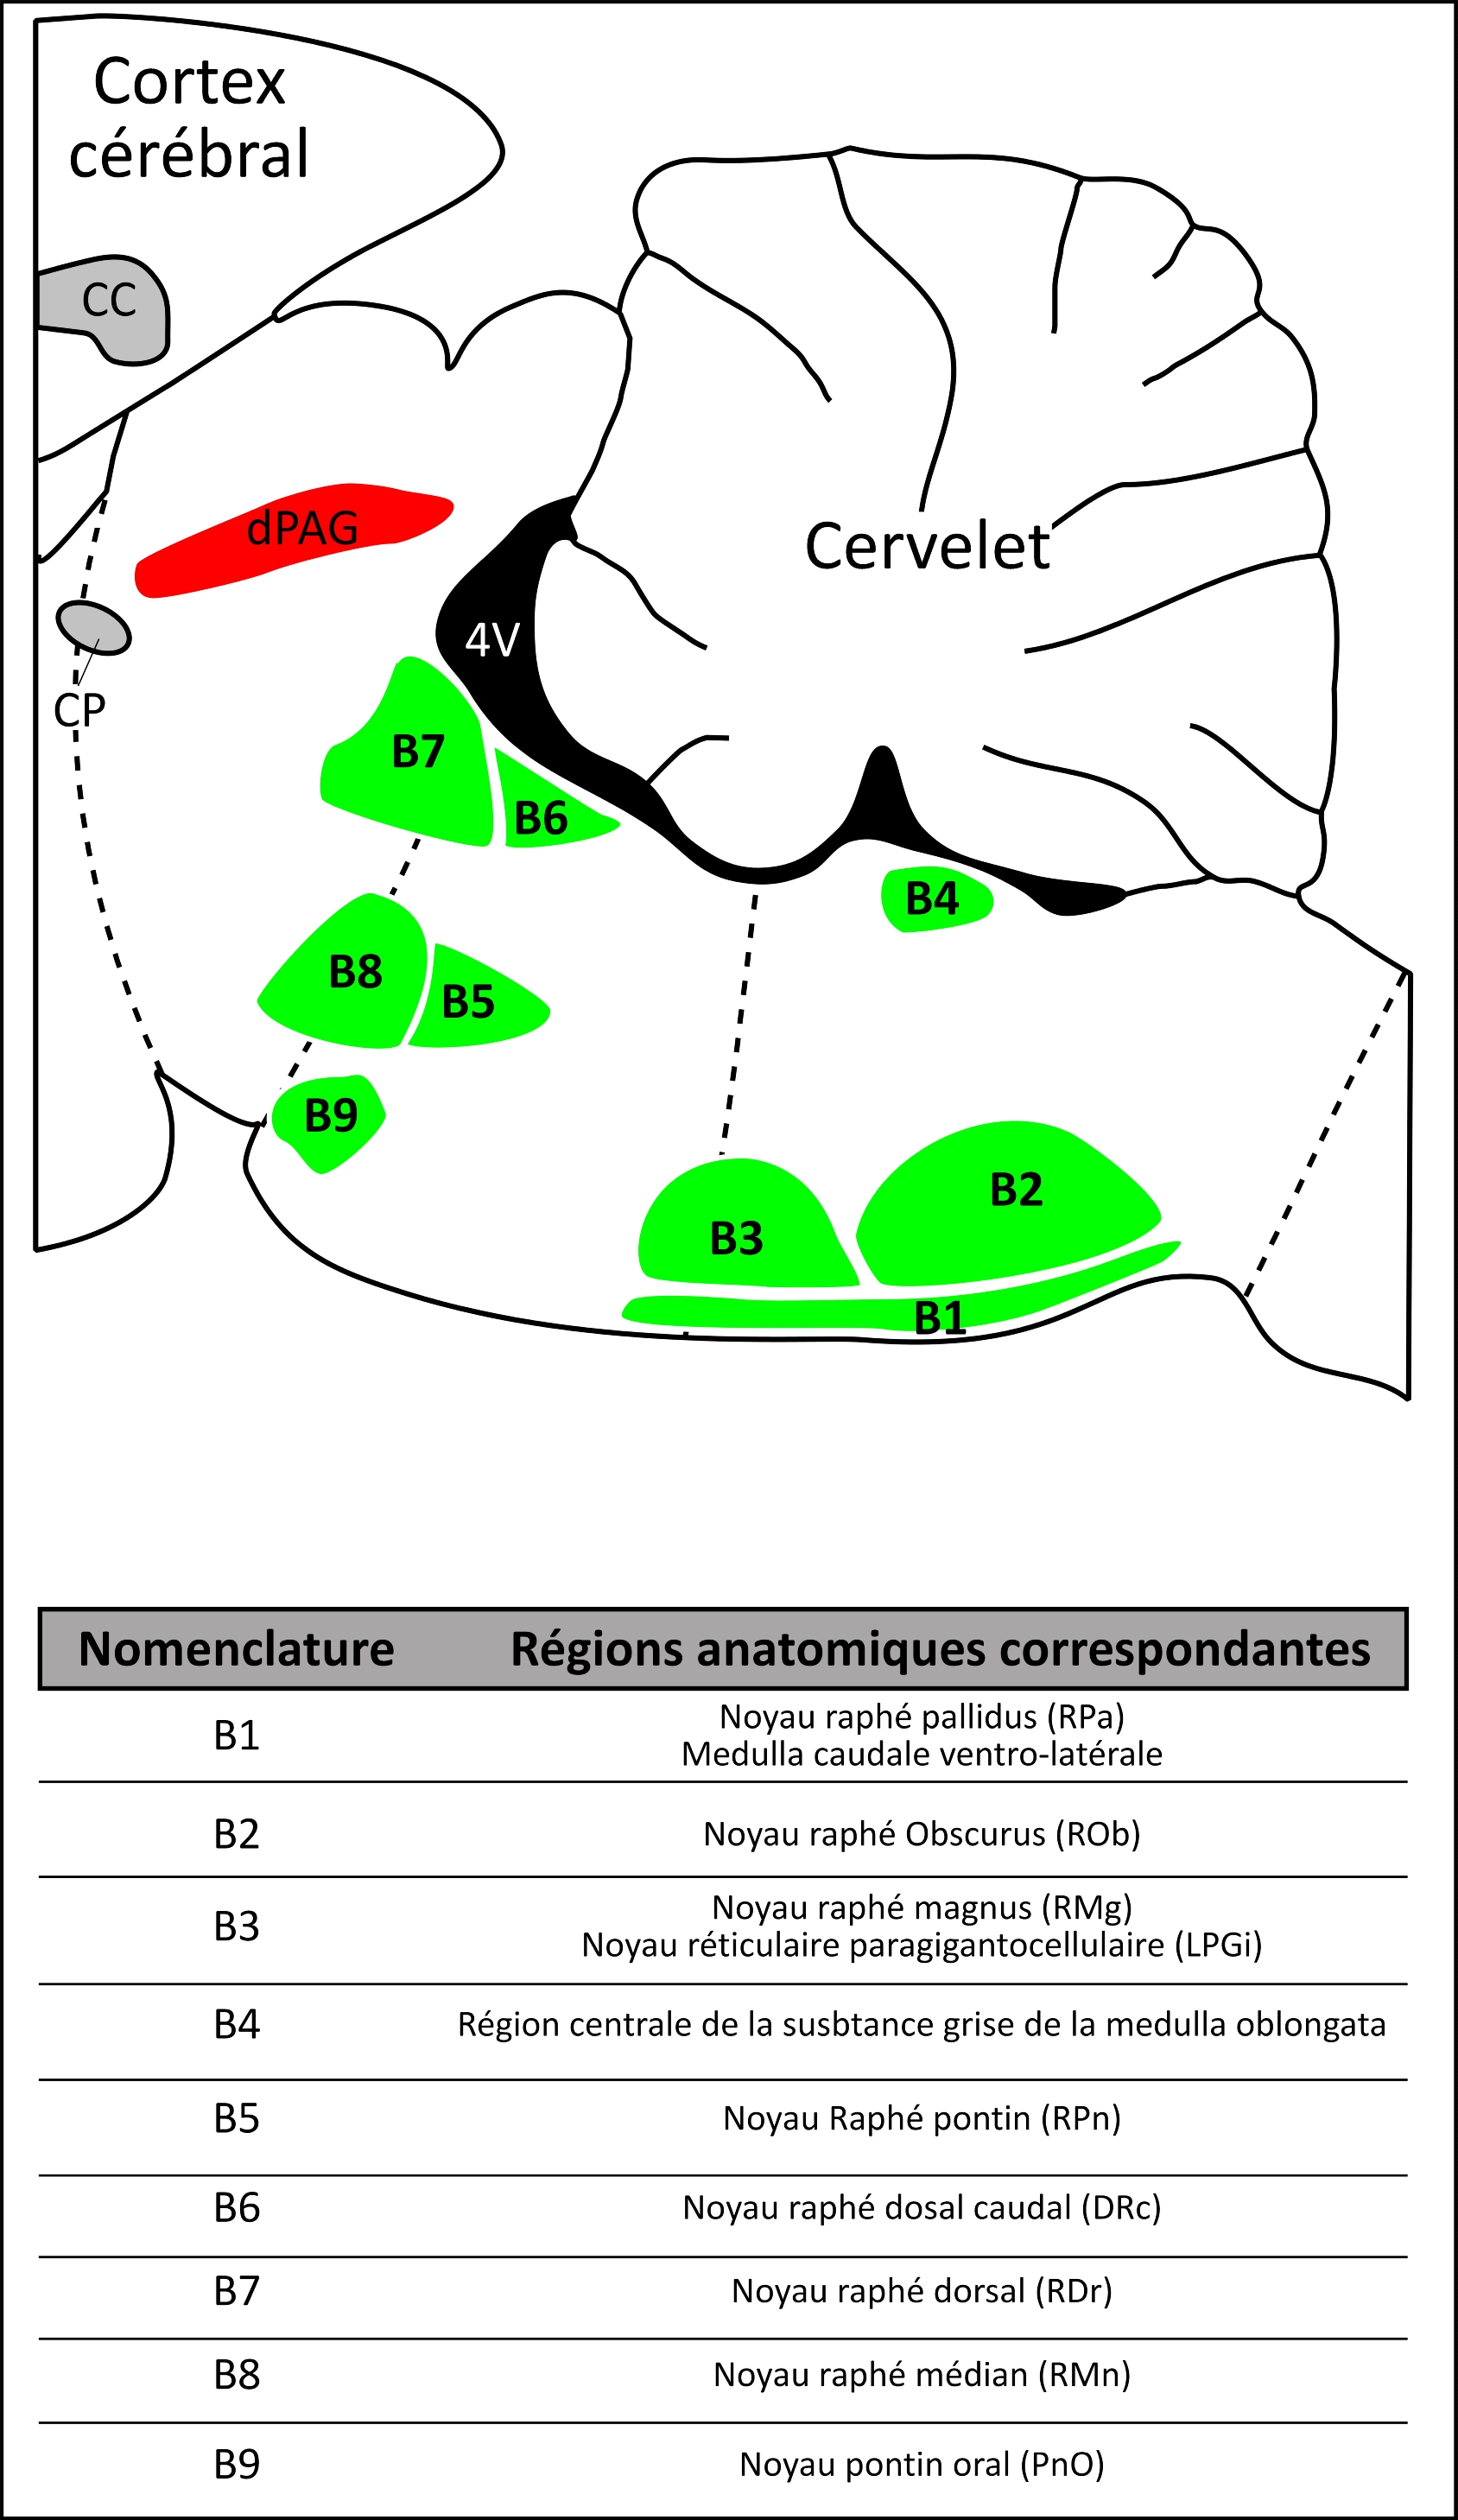
\includegraphics[scale=0.9]{Figure4.jpg} 
\end{center}

\caption{\textbf{Noyaux du raphé}}

{\protect\parbox[t]{18cm}{
\begin{small}
Représentation schématique d’une coupe sagittale de cerveau de rat sur laquelle ont été dessinés les différents noyaux du raphé contenant les somas des neurones sérotoninergiques. Ces groupes de neurones sont notés de B1 à B9 selon l’axe caudorostral (Dahlström et Fuxe, 1964). Une portion de la colonne dorsale de la substance grise périaqueducale (dPAG) a été représentée pour situer l’axe « PAG-RVM/B3 ».\\
4V : 4\textsuperscript{ème} ventricule ; CC : Corps calleux ; CP : Commissure postérieure \end{small}}}

\label{Figure 4}

\end{figure}

\clearpage

\subsubsection{Afférences, projections et transmission synaptique}
\label{Afférences, proj, transmission}

Parmi les différentes afférences de la RVM, toutes les colonnes de la PAG, à l’exception d’une partie de la colonne dorsolatérale, semblent projeter sur les neurones sérotoninergiques du groupe B3 (Lakos \& Basbaum 1988; Braz et al. 2009), même si ceux-ci ne semblent pas être la principale population visée, en tout cas par la PAG ventrolatérale (Morgan et al. 2008). L’utilisation de virus neurotropes conditionnels comme traceur transneuronal a permis de montrer que le groupe B3 reçoit aussi des projections afférentes des cellules catécholaminergiques et non catécholaminergiques des noyaux A5-7, ainsi que du locus coeruleus et subcoeruleus. Des projections afférentes des neurones non cholinergiques du noyau du tegmentum pédonculo-pontin ont également été identifiées. Enfin, le groupe B3 reçoit des afférences oligosynaptiques des neurones sérotoninergiques du raphé dorsal et des couches profondes de la corne dorsale de la moelle épinière (Braz et al. 2009).

Les projections des neurones sérotoninergiques des groupes B1 à B3 sont principalement spinales, via le quadrant dorsolatéral de la moelle épinière (Lakos \& Basbaum 1988; Bullitt \& Light 1989). En fait, la quasi-intégralité des afférences sérotoninergiques spinales provient des groupes B1 à B3, les groupes plus rostraux (B4 à B9) n’y contribuant que de façon très mineure (Oliveras et al. 1977a; Skagerberg \& Bjorklund 1985). Néanmoins, il existe dans la littérature de grandes différences quant à l’évaluation du pourcentage de la composante sérotoninergique au sein des projections spinales. Ainsi, Bowker et Abbott rapportent que 85 \% des projections spinales issues de ces raphés seraient sérotoninergiques et que 90 \% de leurs neurones sérotoninergiques projetteraient sur la moelle (Bowker \& Abbott 1990). D’autres travaux montrent que seulement la moitié des projections spinales sont sérotoninergiques et seul 30 à 60 \% des neurones sérotoninergiques des groupes B1 à B3 sont concernés (Skagerberg \& Bjorklund 1985; Jones \& Light 1990). Enfin, Marinelli et al. (2002) trouvent que seulement 40 \% des projections spinales issues de la RVM sont sérotoninergiques.

En plus de la différence entre cornes dorsales et cornes ventrales décrite plus haut, suggérant que le groupe B3 intervient plus dans les modulations sensorielles et les groupes B1 et B2 plus concernés par la motricité, il faut aussi rappeler que des terminaisons sérotoninergiques ont été mises en évidence dans les cornes intermédiolatérales (Loewy \& McKellar 1981; Allen \& Cechetto 1994), au contact des neurones préganglionnaires sympathiques et des neurones parasympathiques (Helke et al. 1986; Appel et al. 1987; Wu \& Wessendorf 1992; Wu et al. 1993; Nakamura et al. 2004b).

Les neurones du groupe B3 envoient aussi des collatérales dans plusieurs régions du tronc cérébral (Gao \& Mason 1997; 2001b). Ils projettent localement au sein de la RVM elle-même en ciblant préférentiellement les neurones sérotoninergiques (Potrebic et al. 1995), comme décrit préalablement au niveau du raphé dorsal (Wang \& Aghajanian 1978; 1982). Par ailleurs, le groupe B3 projette sur la région ventrolatérale du bulbe (Connelly et al. 1989; Holtman et al. 1990a; Nicholas \& Hancock 1990; Gao \& Mason 1997), le NTS (Thor \& Helke 1987; Schaffar et al. 1988), vers les couches superficielles du noyau trijumeau, ainsi que le noyau ambigu (Haxhiu et al. 1993) et les noyaux moteurs des nerf crâniens V (nerfs trijumeaux), VI (nerfs abducens), VII (nerfs faciaux) et XII (nerfs hypoglosses) (Li et al. 1993a; Manaker \& Tischler 1993). Un même neurone sérotoninergique peut avoir de nombreuses collatérales axonales, qui atteignent à la fois des régions distales, par exemple les cornes intermédiolatérales de la moelle, et des régions plus proches du tronc cérébral (Bowker \& Abbott 1990; Li et al. 1993b; Allen \& Cechetto 1994). 

Il faut noter que la plupart des varicosités terminales sérotoninergiques établit des contacts non synaptiques avec les neurones des cornes dorsales (Marlier et al. 1991a; Ridet et al. 1993). Même si certains neurones sérotoninergiques établissent des contacts synaptiques « classiques » (Jankowska et al. 1995; Maxwell \& Jankowska 1996), la majorité de la transmission sérotoninergique à ce niveau est donc de type « paracrine » (Bunin \& Wightman 1999; Kiss \& Vizi 2001).

\begin{figure}[p]

\begin{center}
 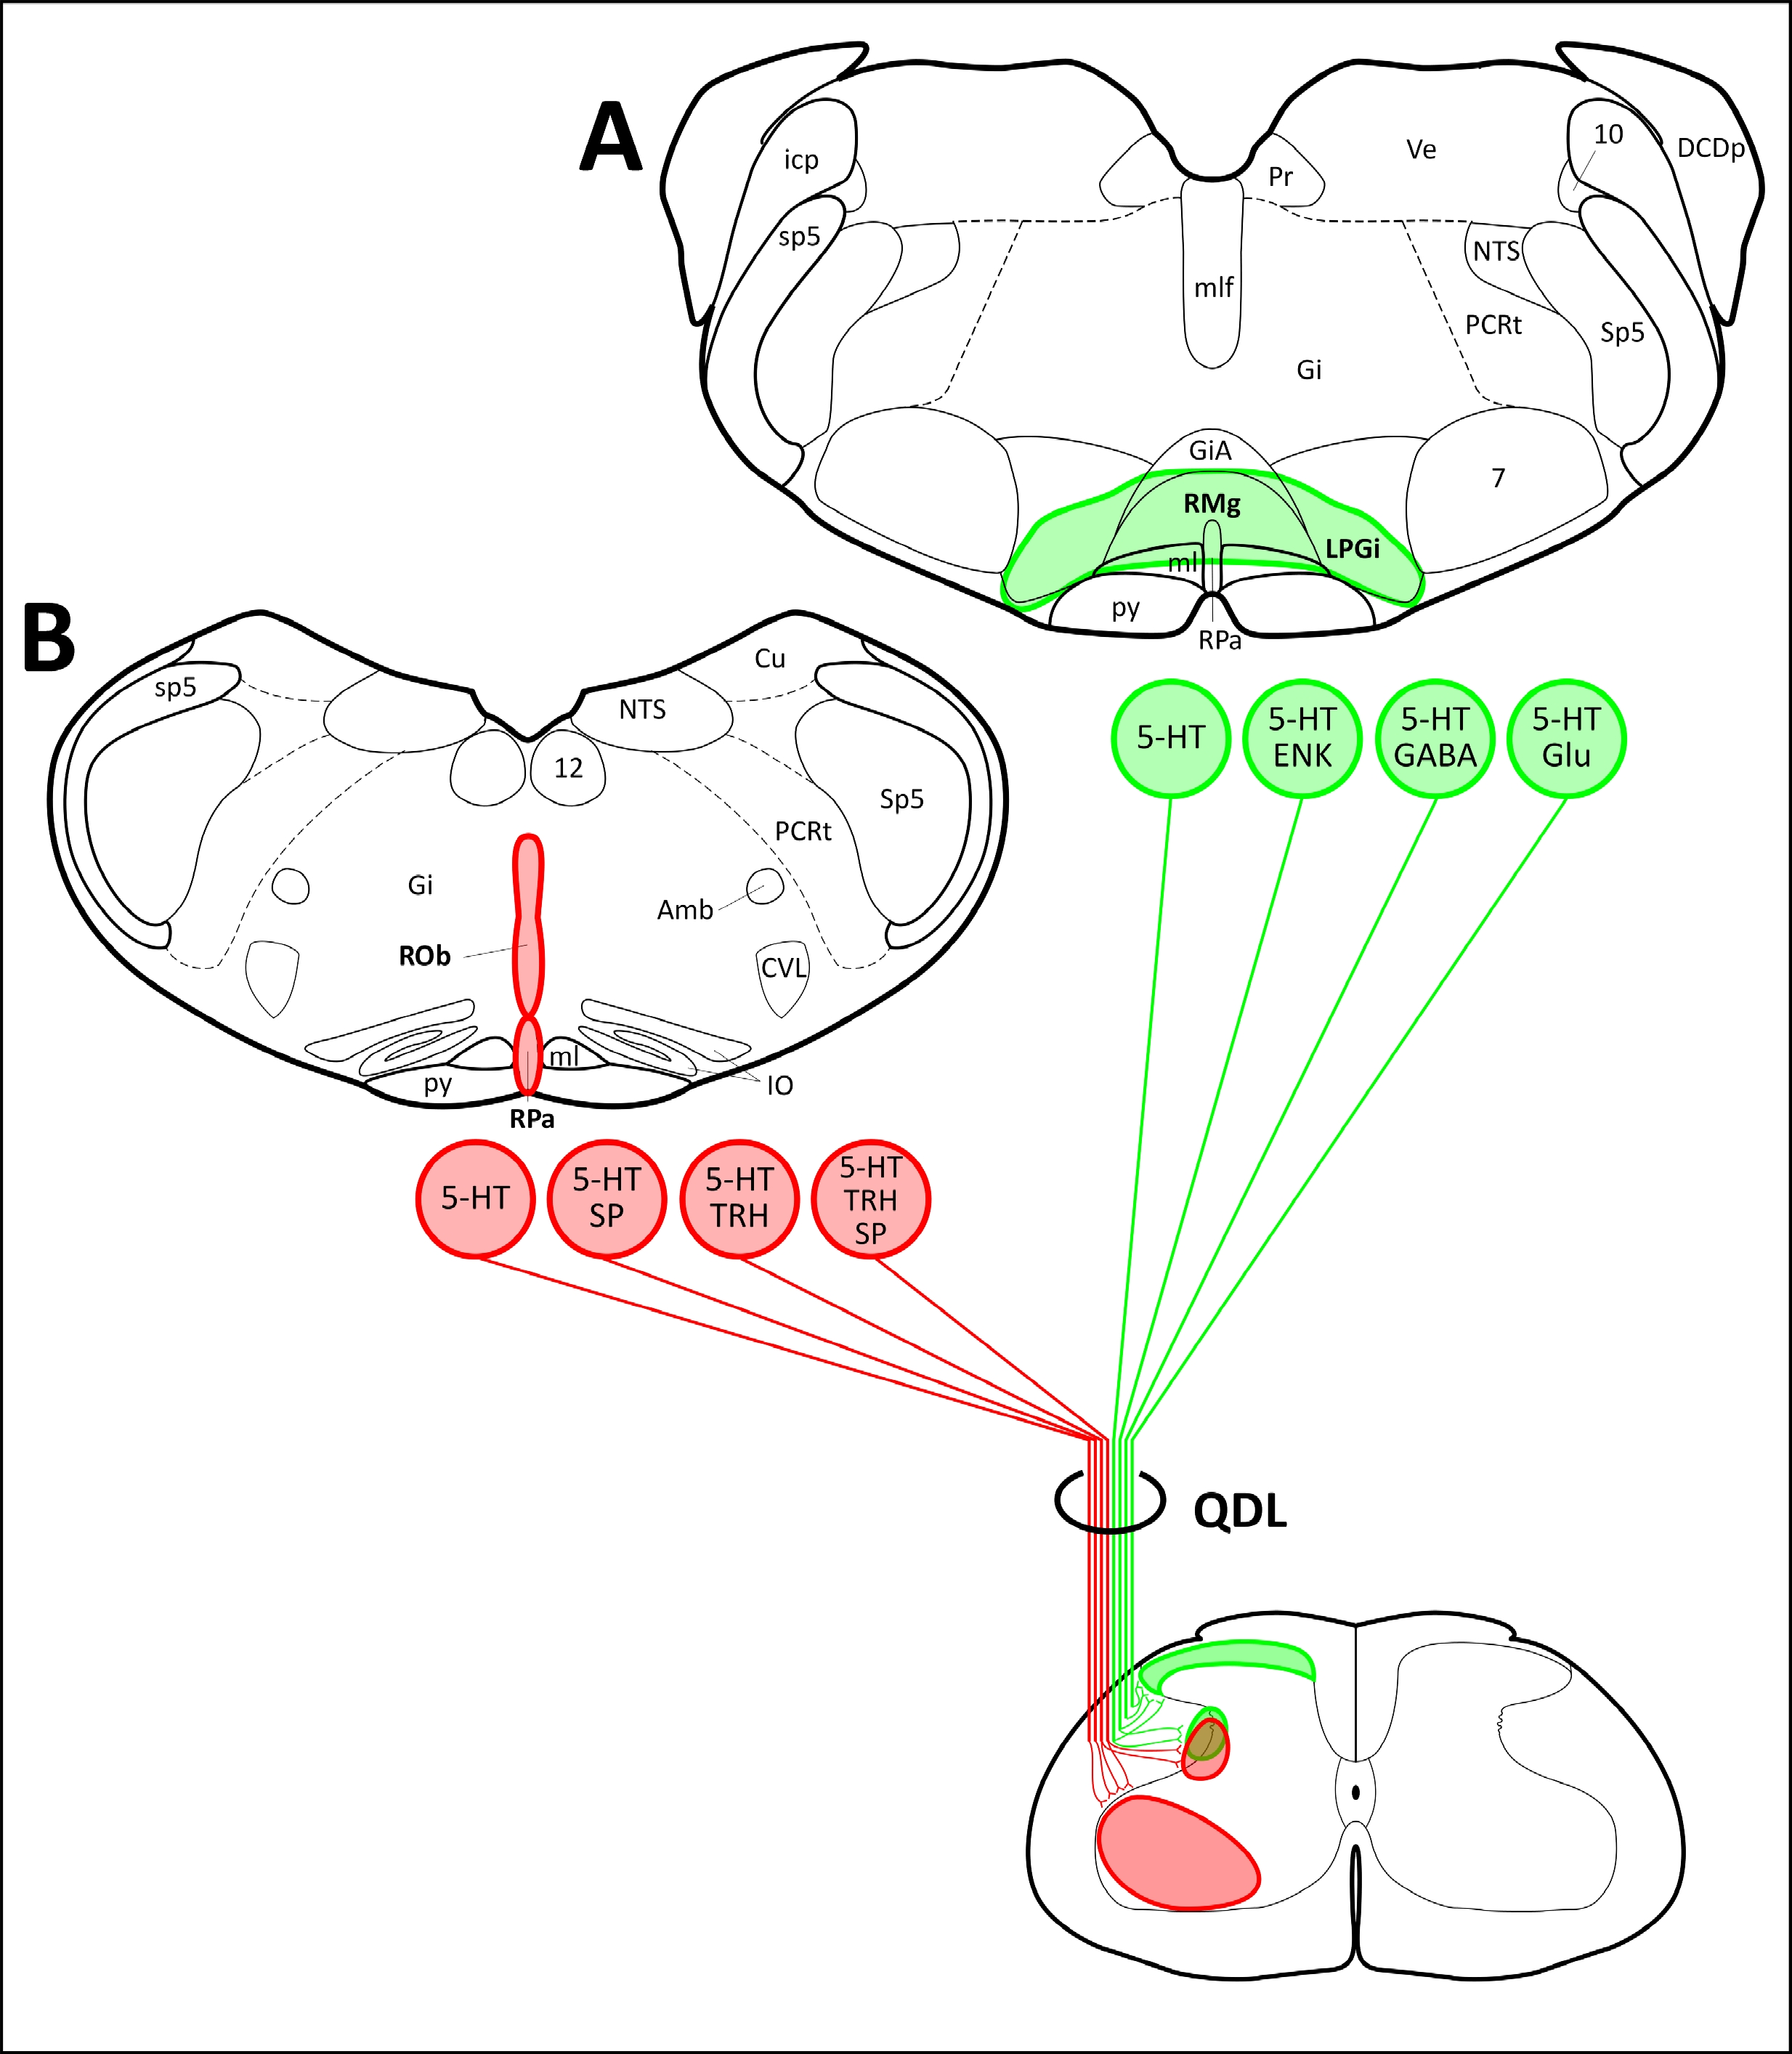
\includegraphics[scale=0.7]{Figure5.jpg} 
\end{center}

\caption{\textbf{Neurochimie et projection de l’« ensemble postérieur » des noyaux du raphé}}

{\protect\parbox[t]{18cm}{
\begin{small}
De nombreux neurones sérotoninergiques du groupe B3 (vert - A) utilisent aussi des acides aminés et des enképhalines comme neurotransmetteur et projettent majoritairement sur les couches superficielles de la corne dorsale. À l’inverse, ceux des groupes B1 et B2 (rouge - B) sont relativement plus riches en peptides et projettent préférentiellement sur la corne ventrale. Les trois groupes projettent aussi sur la corne intermédiolatérale. Les surfaces colorées représentent les régions présentant la plus forte densité de somas sérotoninergiques dans le bulbe (A et B) et de terminaisons sérotoninergiques dans la moelle épinière. Pour la clarté du schéma, les projections spinales n’ont été représentées que d’un seul côté.\\
A : -11,28 mm ; B : -13,20 mm postérieur à bregma ; 5-HT : sérotonine ; 10 : Noyau du nerf vague ; Amb : Noyau ambigu ; Cu : Noyau cunéatus ; CVL : Région caudoventrolatérale du bulbe ; ENK : Enképhalines ; GABA : Acide gamma amino butyrique ; Glu : Glutamate ; Gi : Noyau réticulé gigantocellulaire ; GiA : Noyau réticulé gigantocellulaire pars $\alpha$ ; LPGi : Noyau latéral paragigantocellulaire ; ml : Lémnisque médian ; mlf : Fascicule longitudinal médian ; NTS : Noyau du tractus solitaire ; PCRt : Noyau réticulaire parvicellulaire ; Py : Tractus pyramidal ; QDL : Quadrant dorsolatéral de la moelle épinière ; RMg : Raphé magnus ; ROb : Raphé obscurus ; RPa : Raphé pallidus ; sp5 : Tractus trigéminal spinal ; Sp5 : Noyau du trijumeau ; SP : Substance P ; SRD : Sous-noyau réticulé dorsal ; TRH : \textit{Thyrotropin releasing hormone} ; Autres abréviations : voir liste pages 10-11. Adapté de Hökfelt et al. 2000.
\end{small}}}

\label{Figure 5}

\end{figure}

\clearpage

\subsubsection{Particularités des neurones sérotoninergiques du raphé magnus}

La très grande majorité des études électrophysiologiques des neurones du groupe B3 a en fait concerné ceux du RMg. Il n’existe à ma connaissance qu’une seule étude d’électrophysiologie spécifiquement ciblée sur les neurones sérotoninergiques du LPGi et sur leur chémosensibilité (Mulkey et al. 2004).

Les neurones sérotoninergiques du RMg ont quelques spécificités. Tout d’abord, ils ont la fréquence de décharge la plus élevée des neurones sérotoninergiques (Dickenson 1977; Auerbach et al. 1985; Fornal et al. 1985). Ensuite ces neurones sérotoninergiques bulbaires semblent moins sensibles aux agonistes 5-HT$_{1A}$ que les autres neurones sérotoninergiques (Heym et al. 1982b; Jacobs et al. 1983; Fornal et al. 1985). De fait, leur niveau d’expression des autorécepteurs 5-HT$_{1A}$ est plus faible à ce niveau (Helke et al. 1997; Zhang et al. 2000a; Bonnavion et al. 2010).

Les études chez le chat éveillé
\footnote{Toutes les études équivalentes faites chez le rat ont été incapables d’enregistrer des neurones ayant les caractéristiques électrophysiologiques « classiques » des neurones sérotoninergiques (Martin et al. 1992; Leung \& Mason 1999). La seule mention de neurones lents et réguliers que j’ai pu trouver dans des études chez le rat non-anesthésié est la suivante : « […] \textit{we have also recorded a few other different units exclusively under morphine, such as five units with a very slow, regular spontaneous activity (about 2 Hz), not modified by peripheral stimuli, and only one neuron specifically excited by a non-noxious stimulus.} » (Martin et al. 1992). En réalité, comme suggéré par certains auteurs, il est très probable que le type d’électrode utilisé dans ces études chez le rat non-anesthésié ne permettent pas d’enregistrer des neurones lents et réguliers (Leung \& Mason 1999).}
ont montré que contrairement à l’activité des neurones sérotoninergiques des raphés médian et dorsal, celle des neurones sérotoninergiques du RMg n’est pas corrélée à l’occurrence de certaines activités phasiques du sommeil (i.e. ondes ponto-géniculo-occipitales et fuseaux) (Fornal et al. 1985).

Enfin, plus récemment, des d’études d’électrophysiologie \textit{in-vitro} sur tranches ont permis d’identifier 3 sous-populations de neurones sérotoninergiques du RMg projetant vers la moelle (Zhang et al. 2006; Zhang \& Hammond 2010). La distinction entre ces 3 groupes porte essentiellement sur leurs caractéristiques de décharge spontanée (et de potentiel de repos, de capacitance membranaire\ldots) mais a une réelle signification pharmacologique et fonctionnelle (voir « \ref{Neurones 5-HT du RMg : effets de la nociception} Neurones sérotoninergiques du raphé magnus : effets de la nociception » - page \pageref{Neurones 5-HT du RMg : effets de la nociception} et « \ref{Role de la 5-HT dans analgésie opioidergique} Rôle de la sérotonine dans l'analgésie induite par les opioïdes » - page \pageref{Role de la 5-HT dans analgésie opioidergique}). On distingue ainsi :

\begin{itemize}
\item les neurones de type 1 dont l’activité spontanée est lente ($\approx$ 1 Hz) et relativement irrégulière,
\item les neurones de type 2 qui n’ont aucune activité spontanée,
\item les neurones de type 3 dont l’activité spontanée est moins lente ($\approx$ 3 Hz) et régulière.
\end{itemize}

L’activité spontanée des types 1 et 3 a une origine endogène et n’est pas le résultat d’une activité de réseau excitatrice. L’absence d’activité du type 2 n’est pas explicable par un tonus inhibiteur au sein de la tranche, mais pourrait résulter de la déafférentation inhérente à cette préparation
\footnote{L’activité rythmique de certains neurones sérotoninergiques pourrait avoir une origine « exogène » (i.e, le résultat de l’activité rythmique de certaines afférences) ou « endogène », mais sous certaines conditions : l’activité rythmique de la plupart des neurones sérotoninergiques du raphé dorsal ne se manifeste \textit{in-vitro} qu’en présence d’agonistes $\alpha_{1}$ adrénergiques (Vandermaelen \& Aghajanian 1983).}. 
Toutefois, certains arguments tendent à montrer que ces neurones pourraient bien exister \textit{in-vivo}. Quelques études ont montré l’existence de neurones silencieux avec des vitesses de conduction faible (Wessendorf et al. 1981; Wessendorf \& Anderson 1983) et de longs potentiels d’action (Nalivaiko \& Blessing 2002) : deux caractéristiques des neurones sérotoninergiques. De plus, le nombre de ces neurones diminue à la suite d’un traitement à la 5,7-DHT, suggérant qu’une partie au moins de ces neurones silencieux pourrait être sérotoninergique (Wessendorf et al. 1981).

\subsection{Neurones sérotoninergiques du raphé magnus : effets de la nociception}
\label{Neurones 5-HT du RMg : effets de la nociception}

Plusieurs travaux d’électrophysiologie \textit{in-vivo} ont étudié directement la réponse des neurones sérotoninergiques du RMg à des stimulations nociceptives.

Chez le chat éveillé, ces neurones répondent pour partie à des stimulations nociceptives (Auerbach et al. 1985)
\footnote{Il semblerait que la moitié de ces neurones répondent de manière phasique à des stimulations visuelles ou auditives simples (Fornal et al. 1985)}. 
Alors que la décharge de ces neurones ne semble pas être affectée par une injection s.c. de formaline, la moitié d’entre eux répondent à des stimulations nociceptives mécaniques et 40 \% à des stimulations nociceptives thermiques. Néanmoins, les auteurs concluent que l’activation de ces neurones par ces stimulations est surtout liée à la réaction d’éveil (mesuré par l’EEG) qu’elles engendrent car :

\begin{itemize}
\item les réponses de ces neurones à des stimuli nociceptifs sont plus fréquentes lorsque la stimulation déclenche aussi une désynchronisation de l’activité corticale, et que
\item ces mêmes neurones sont activés par des stimuli environnementaux qui déclenchent une réaction d’éveil (Auerbach et al. 1985). 
\end{itemize}

Chez le rat anesthésié, les études utilisant seulement des méthodes indirectes d’identification des neurones sérotoninergiques donnent des résultats assez hétérogènes. Certains auteurs rapportent que les neurones sérotoninergiques du RMg ne répondent pas aux stimulations nociceptives (Dickenson 1977). Pour leur part, Wessendorf \& Anderson (1983), se basant sur la seule vitesse de conduction comme critère d’identification, concluent que la majorité de ces neurones sont activés par des stimulations nociceptives mécaniques, mais relativement insensibles à des stimulations nociceptives thermiques.

En se basant à la fois sur leur vitesse de conduction et sur leur fréquence de décharge spontanée, Chiang \& Gao (1986) rapportent que les deux tiers des neurones sérotoninergiques du RMg sont activés par des stimulations nociceptives thermiques et mécaniques, alors que le dernier tiers est inhibé. Une étude plus récente a montré que des neurones, classés comme sérotoninergiques par les auteurs, en fonction de leurs potentiels d’action de longue durée et leur faible vitesse de conduction mais sans activité spontanée, (pouvant donc correspondre aux neurones sérotoninergiques de type 2 identifiés in-vitro ; voir ci-dessus), ne répondent pas aux stimulations nociceptives mécaniques (Nalivaiko \& Blessing 2002).

Les études utilisant des méthodes immunohistochimiques d’identification des neurones sérotoninergiques enregistrés ont, quant à elles, donné des résultats plus cohérents. Ainsi Potrebic et al (1994) ont, pour la première fois, montré que les neurones directement identifiés comme sérotoninergiques étaient quasi insensibles à des stimulations thermiques et mécaniques. Ce résultat a été confirmé par la suite par d’autres groupes (Winkler et al. 2006), et surtout par Mason et collaborateurs dans plusieurs études, et sur de plus grands échantillons de cellules (Gao et al. 1997; Mason 1997; Gao et al. 1998; Leung \& Mason 1998; Gao \& Mason 2001b; Brink \& Mason 2003). Il ressort de ces études que :

\begin{itemize}
\item les réponses de ces neurones sont en général de faible amplitude et limitées à la durée du stimulus (Gao et al. 1997; Mason 1997; Gao et al. 1998; Leung \& Mason 1998; Gao \& Mason 2001b; Brink \& Mason 2003) ;
\item 78 \% des neurones sérotoninergiques du RMg sont insensibles à une stimulation nociceptive thermique de la queue et que seulement 17 \% sont activés et \item 5 \% inhibés (Gao \& Mason 2000) ;
\item 20 \% de ces neurones sont activés par une stimulation nociceptive mécanique mais pas thermique (Mason 1997) ;
\item 71 \% de ces neurones sont insensibles à une distension colorectale. Seulement 13 \% sont activés et 17 \% inhibés (Brink \& Mason 2003). De plus il n’y a pas de lien entre l’effet d’une stimulation viscérale et celui d’une stimulation somatique sur un même neurone (Gao \& Mason 2001b; Brink \& Mason 2003).
\end{itemize}

Bien qu’aucune étude électrophysiologique n’ait été consacré à l’analyse des effets de stimulations nociceptives prolongées sur les neurones sérotoninergiques du groupe B3, l’utilisation de méthodes indirectes (voltamétrie et/ou quantification par chromatographie) a permis de montrer que certains types de stimulations nociceptives pouvaient augmenter la libération de sérotonine dans la RVM ou au niveau des cornes dorsales. C’est notamment le cas d’injections intradermales de formaline, de capsaïcine ou de carragénine chez l’animal anesthésié ou éveillé (Puig et al. 1992; Sorkin \& McAdoo 1993; Taylor \& Basbaum 1995; Zhang et al. 2000b). Dans un deuxième temps, le suivi de marqueur indirect de l’activité ou de plasticité neuronale (ERK, p-38 MAPK, c-fos) a permis de confirmer l’activation de certains neurones sérotoninergiques du RMg à la suite d’injections intradermales de formaline ou dans des modèles de douleurs inflammatoires (Suzuki et al. 2002; Imbe et al. 2005; Imbe et al. 2007). Ces résultats sont cohérents avec les données d’électrophysiologie \textit{in-vitro} montrant une augmentation de la décharge spontanée des neurones sérotoninergique de type 3 (lent et régulier) après 4 jours d’inflammation (Zhang \& Hammond 2010). 

\subsection{Rôle de la sérotonine dans les contrôles descendants }
\label{5-HT dans contrôle descendants}

Initialement, l'effet « antinociceptif » de l’axe « PAG-RVM-corne dorsale » impliquait que les neurones sérotoninergiques du RMg activés par une stimulation de la PAG inhibaient la transmission des \textit{inputs} nociceptifs au niveau des couches superficielles de la corne dorsale (Basbaum \& Fields 1978; Fields \& Basbaum 1978). Ce schéma est supporté par plusieurs arguments :

\begin{itemize}
\item On observe une libération de sérotonine au niveau de la moelle lors de stimulations électriques antinociceptives du RMg (Bourgoin et al. 1980; Rivot et al. 1982; Hentall et al. 2006) ou de la PAG (Cui et al. 1999). 
\item L’effet antinociceptif d’une stimulation électrique de la PAG est diminué par un traitement à la pCPA (Akil \& Mayer 1972; Akil \& Liebeskind 1975; Carstens et al. 1981). Un effet similaire est obtenu après l’injection systémique (Yezierski et al. 1982b) ou i.t. d’antagonistes sérotoninergiques (Yaksh et al. 1976; Yaksh \& Wilson 1979).
\item De même, les effets analgésiques de stimulations électriques du RMg sont diminués par un traitement à la pCPA (Rivot et al. 1980), l’injection systémique (Yezierski et al. 1982b; Paul \& Phillips 1986) ou i.t. d’antagonistes sérotoninergiques (Yezierski et al. 1982b; Satoh et al. 1983; Hammond \& Yaksh 1984; Barbaro et al. 1985; Zhuo \& Gebhart 1991; McGowan \& Hammond 1993b) ou encore par l’inhibition de l’expression de la TPH2 dans les neurones du RMg par la production locale d’ARN interférents (Wei et al. 2010).
\end{itemize}

Cependant, plusieurs données sont incompatibles avec une inhibition phasique par la sérotonine :

\begin{itemize}
\item L’augmentation de la libération de sérotonine au niveau des cornes dorsales de la moelle épinière n’est pas systématiquement liée aux effets antinociceptifs d’une stimulation du RMg (Sorkin et al. 1993). 
\item Les études électrophysiologiques suggèrent que les neurones sérotoninergiques du RMg activés de façon directe par des stimulations de la PAG sont apparemment très rares.
\begin{itemize}
\item La première étude, chez le chat éveillé, a montré que presque tous les neurones présumés sérotoninergiques étaient activés par des stimulations antinociceptives de la PAG (Auerbach et al. 1985). Toutefois, la durée des latences de la réponse orthodromique de ces neurones fait dire aux auteurs que cette activation est probablement polysynaptique (Auerbach et al. 1985). 
\item La deuxième étude, chez le chat anesthésié, a montré qu’aucun des neurones du RMg étudié présentant des PPSE monosynaptiques en réponse à une stimulation électrique de la PAG n’était sérotoninergique (Mason et al. 1988). 
\item La troisième étude, chez le rat anesthésié et combinant identification directe (immunohistochimique) et indirecte (selon des critères de décharges spontanée) des neurones sérotoninergiques du RMg, a montré qu’aucun des neurones enregistrés n’était activé par des stimulations ou des trains de stimulations de la PAG (Gao et al. 1997).
\end{itemize}
\end{itemize}

\bigskip 

Pour résoudre ce dilemme, certains auteurs ont suggéré que la sérotonine inhiberait de façon tonique la transmission nociceptive (Mason \& Gao 1998) en arguant que son action spinale est principalement antinociceptive (Yaksh \& Wilson 1979) puisque son application iontophorétique inhibe la réponse des neurones des cornes dorsales à des stimulations nociceptives (Randic \& Yu 1976; Belcher et al. 1978; Jordan et al. 1978). Mais cette hypothèse aussi semble contredite par le fait que des souris dépourvues de neurones sérotoninergiques et des rats dont l’activité TPH2 des neurones sérotoninergiques du RMg a été considérablement réduite par des ARN interférents, ont des réactions normales à des stimulations nociceptives brèves (Zhao et al. 2007; Wei et al. 2010). 

\bigskip

Outre son action inhibitrice sur la nociception, la sérotonine semble aussi posséder un potentiel pronociceptif. En effet, certains auteurs soulignent que les neurones sérotoninergiques du groupe B3 sont activés par des stimulations nociceptives prolongées, et que cette activation jouerait un rôle dans le développement des douleurs chroniques (Suzuki et al. 2002; Suzuki et al. 2004b; Suzuki et al. 2005). En fait, l’administration i.t. de faibles doses de sérotonine a des effets antinociceptifs vis-à-vis des douleurs provoquées par une injection intradermale de formaline, alors que des doses plus fortes ont plutôt des effets pronociceptifs dans un même modèle expérimental (Oyama et al. 1996). Un autre argument en faveur d’une action pronociceptive de la sérotonine est que les réponses des neurones des cornes dorsales sont augmentées chez des animaux dépourvus de sérotonine au niveau spinal après une injection i.t. de 5,7-DHT (Rahman et al. 2006). Cet effet pronociceptif pourrait jouer un rôle important au regard de certains types de stimulation nociceptives comme, par exemple, dans le test à la formaline : le nombre de réponses comportementales nociceptives observées pendant ce test est nettement diminué chez des rats dont l’activité TPH2 des neurones sérotoninergiques du RMg a été diminuée par des ARN interférents (Wei et al. 2010) ou chez des animaux ayant reçu un injection de 5,7-DHT dans la RVM (Fasmer et al. 1985). Enfin, cet effet pronociceptif serait aussi impliqué dans les douleurs inflammatoires et neuropathiques car l’inactivation de la TPH2 dans le RMg réduit considérablement le nombre de réponses comportementales nociceptives observées après un traitement avec l’adjuvant complet de Freund, ou à la suite d’une ligature de nerf (Wei et al. 2010). Des observations du même type ont été rapportées à la suite d’injections i.t. de 5,7-DHT (Oatway et al. 2004; Rahman et al. 2006), celle-ci causant une baisse des réponses des neurones des cornes dorsales à des stimulations nociceptives (Rahman et al. 2006).

\bigskip

En conclusion, évaluer l’importance physiologique réelle des modulations positives ou négatives de la nociception par la sérotonine s’avère encore bien difficile. D’ailleurs, les travaux visant à étudier son action centrale avec des méthodologies simples n’ont donné que des résultats nuancés et souvent contradictoires (Le Bars 1988).
 
Plusieurs pistes peuvent être avancées pour rendre compte de ces résultats. Tout d’abord, la sérotonine intervient dans de nombreux phénomènes physiologiques, et les effets d’une altération de la transmission sérotoninergique sur la nociception pourraient être secondaires à la modification d’une autre variable, sans rapport direct avec la nociception per se. À cet égard, il convient de souligner que les études de la nociception chez l’animal se basent sur des réactions motrices, alors que la sérotonine est elle-même directement impliquée dans la modulation de la motricité (Le Bars 1988). Ensuite, la libération de sérotonine au niveau de la corne dorsale a des effets variables en fonction du type de neurone (Lu \& Perl 2007), de récepteurs et de stimulations nociceptives considérés (Bardin et al. 1997a). De plus, les effets de la sérotonine peuvent être différents en fonction des circonstances physiopathologiques. Ceci explique, en partie, que les effets de la sérotonine aient d’abord été vus comme principalement inhibiteurs (Basbaum \& Fields 1978; Yaksh \& Wilson 1979; Basbaum \& Fields 1984; Fields et al. 1991; Furst 1999) et qu’aujourd’hui, elle est davantage considérée comme un modulateur pouvant participer, non seulement à l’analgésie, mais aussi à l’installation et au maintien de différents types de douleurs chroniques (Suzuki et al. 2004b; Bannister et al. 2009). 

\subsection{Rôle de la sérotonine dans l'analgésie induite par les opioïdes}
\label{Role de la 5-HT dans analgésie opioidergique}

Le rôle de la sérotonine et des neurones sérotoninergiques du groupe B3 dans l’analgésie morphinique a longtemps été, et est toujours, sujet à controverse. Il n’en reste pas moins que les neurones sérotoninergiques du groupe B3 expriment plusieurs récepteurs opioïdergiques :

\begin{itemize}
\item La moitié des neurones sérotoninergiques bulbo-spinaux exprime l’ARNm et la protéine du récepteur opioïdergique µ (Kalyuzhny et al. 1996; Wang \& Wessendorf 1999). Cette donnée est cohérente avec la baisse de l’expression cet ARNm observée dans les noyaux du raphé chez des souris dépourvues de neurones sérotoninergiques (Zhao et al. 2007).
\item Environ 75 \% des neurones sérotoninergiques bulbo-spinaux expriment le récepteur opioïdergique $\delta$ (Wang \& Wessendorf 1999). 
Bien que le récepteur $\kappa$ est majoritairement exprimé par des neurones GABAergiques dans la RVM (Winkler et al. 2006), il en existe aussi sur les neurones sérotoninergiques de cette région projetant sur les cornes dorsales 
\item De nombreux neurones sérotoninergiques du groupe B3 sont entourés de varicosités exprimant le récepteur $\delta$ (Arvidsson et al. 1995a) ; c’est notamment le cas pour la moitié de ceux qui projettent sur les cornes dorsales (Kalyuzhny et al. 1996). 
\item Les études d’électrophysiologie \textit{in-vitro} ont montré que ces récepteurs sont fonctionnels, puisque les neurones sérotoninergiques répondent à un et, parfois, à plusieurs types d’agonistes opioïdergiques (Marinelli et al. 2002; Finnegan et al. 2004; Marinelli et al. 2005; Zhang et al. 2006). Zhang et Hammond ont montré que, en fait, seuls les neurones sérotoninergiques de type 1 (i.e. irréguliers) et, dans une moindre mesure, ceux de type 2 (i.e. silencieux) sont concernés, les neurones de type 3 (i.e. réguliers) étant insensibles à ces agonistes (Zhang et al. 2006; Zhang \& Hammond 2010).
\end{itemize}

Au vu de ces données, certaines observations concernant l’implication de la sérotonine dans l’analgésie morphinique semblent cohérentes :

\begin{itemize}
\item L’injection systémique, i.c.v., ou dans la PAG, d’agonistes opioïdergiques µ entraîne, dans certaines conditions, la libération de sérotonine au niveau de la corne dorsale de la moelle épinière (Shiomi et al. 1978; Yaksh \& Tyce 1979; Matos et al. 1992) ou dans la RVM (Rivot et al. 1988; Taylor \& Basbaum 2003). 
\item Les effets analgésiques de la morphine administrée par voie systémique, i.c.v., ou injectée directement dans la RVM, peuvent être partiellement bloqués par une injection de 5,7-DHT au niveau spinal (Kuraishi et al. 1983) ou dans la RVM (Deakin \& Dostrovsky 1978; Mohrland \& Gebhart 1980; Vasko et al. 1984), ainsi que par l’injection systémique (Dickenson et al. 1979; Paul \& Phillips 1986), ou i.t. d’antagonistes sérotoninergiques (Wigdor \& Wilcox 1987).
\item La diminution des effets analgésiques des agonistes opioïdergiques µ et $\delta$, et l’abolition de ceux des agonistes $\kappa$, chez des souris dépourvues de neurones sérotoninergiques (Zhao et al. 2007), corrobore l’idée d’un rôle majeur de la sérotonine dans l’analgésie morphinique.
\end{itemize}

\bigskip 

Toutefois, d’autres observations vont à l’encontre de cette idée. Ainsi, un traitement à la pCPA et l’administration de certains antagonistes sérotoninergiques, sont sans effet ou peuvent même potentialiser l’action antinociceptive de la morphine (pour revue voir Le Bars 1988). D’autre part, la morphine semble incapable de déclencher la libération de sérotonine quand elle est administrée au niveau spinal (Bineau-Thurotte et al. 1984; Vasko et al. 1984; Monroe et al. 1986) ; d’ailleurs, cette libération n’est pas nécessaire aux effets antinociceptifs de la morphine (Chiang \& Xiang 1987; Matos et al. 1992). Plus récemment, il a été montré que la diminution de l’activité de la TPH2 dans les neurones sérotoninergiques du RMg par des ARN interférents, n’affecte pas les effets antinociceptifs d’agonistes µ ou $\kappa$ injectés directement dans la RVM (Wei et al. 2010). Enfin, les études d’électrophysiologie \textit{in-vivo} montrent que la morphine systémique n’a pas d’effet sur la majorité des neurones sérotoninergiques du RMg. Seule une minorité d’entre eux est activée ou inhibée (voir Tableau \ref{Tableau 1} - page \pageref{Tableau 1}) (Auerbach et al. 1985; Chiang \& Pan 1985; Gao et al. 1998), sans que cela change le niveau de décharge de l’ensemble de la population (Auerbach et al. 1985; Gao et al. 1998). De plus, l’activation ou l’inhibition est généralement de courte durée et sans lien avec le niveau d’analgésie ou la réponse de ces neurones à des stimulations nociceptives
\footnote{Même si, concordant partiellement avec les études \textit{in-vitro}, les cellules affectées par la morphine ont une décharge plus irrégulière que celle qui y sont insensibles (Gao et al. 1998).} 
(Gao et al. 1998).

\begin{sidewaystable}
% \documentclass[a4paper,12pt,twoside]{report}
% 
% \usepackage[utf8x]{inputenc}
% %\usepackage[latin1]{inputenc}
% \usepackage[T1]{fontenc}
% \usepackage[francais]{babel}
% 
% \usepackage{setspace} % Interligne
% %\singlespacing
% %\onehalfspacing
% \doublespacing
% 
% \usepackage{soul} % Pour souligner ou barrer du texte
% \usepackage{ulem}
% 
% \usepackage{textcomp}
% 
% \usepackage{wrapfig} % pour encadrer les figures avec du texte
% \usepackage{graphicx}
% 
% \usepackage{multicol} % Pour utiliser l'environnement multicol
% \setlength\columnseprule{.4pt} % Pour mettre un trait séparateur de colonnes\usepackage{multirow} % Pour fusionner les lignes dans les tableaux
% 
% \usepackage{array} % Pour centrer les lignes en hauteur dans un tableau
% \usepackage{rotating} % Pour tourner un tableau
% 
% \usepackage[table]{xcolor} %Pour colorer des cellules
% 
% \usepackage{xcolor}
% \usepackage{colortbl}
% 
% 
% \begin{document}
% \begin{sidewaystable}

\setlength{\tabcolsep}{1pt}
\centering
\caption{\textbf{Réponses des neurones 5-HT du RMg à la morphine administrée par voie systémique}}
\setlength\minrowclearance{6pt}

\newcolumntype{A}{%
>{\centering}%
m{2.8cm}}

\newcolumntype{D}{%
>{\centering\bfseries}%
m{2.8cm}}

{%
\newcommand{\mc}[3]{\multicolumn{#1}{#2}{#3}}

\begin{tabular}{|A|A|m{6.5cm}|A|D|D|D|c}
\hline
\textbf{Études}			&\textbf{Modèle expérimental}				&\centering\textbf{Identification des neurones}										&\textbf{Morphine}		& Insensibles		&Inhibés	&Activés&	\\ \hline
Auerbach et al. \newline1985 	&Chat éveillé 						& Pattern de décharge \newline\footnotesize (lent, régulier, inactifs pendant le sommeil) \newline Pharmacologique 	&2 mg/kg \newline i.p. 		& \multicolumn{2}{c|}{\textbf{15}} 	&1	&	\\ \hline
Chiang \& Pan\newline1985	&Rat anesthésié \footnotesize uréthane 1,1 g/kg 	& Pattern de décharge \newline\footnotesize (lent, régulier) \newline Conduction lente 					&5 mg/kg \newline i.p. 		& 6 		& 3 			&1	&	\\ \hline
Gao et al. \newline1998 	&Rat anesthésié \footnotesize halothane 1\% 		& Pattern de décharge \newline\footnotesize (lent, régulier) \newline Immunohistochimique 				&0,5-10 mg/kg \newline s.c. 	& 20		& 6 			&6	&	\\ \hline
\end{tabular}

}
% \end{sidewaystable}
% \end{document}

 \label{Tableau 1}
\end{sidewaystable}

\subsection{Implication des récepteurs sérotoninergiques dans la transmission nociceptive}
\label{Implication des récepteurs 5-HT dans la transmission nociceptive}

Il a été dénombré à ce jour au moins quinze types de récepteurs de la sérotonine répartis en sept classes : de 5-HT$_{1}$ à 5-HT$_{7}$ (Boess \& Martin 1994; Barnes \& Sharp 1999).

Tous ces récepteurs, à l’exception des récepteurs 5-HT$_{3}$, sont des récepteurs métabotropiques appartenant à la superfamille des récepteurs couplés aux protéines G (Barnes \& Sharp 1999). Les récepteurs 5-HT$_{1}$ ont une affinité nanomolaire pour la sérotonine (Hoyer 1988), alors que les autres récepteurs se caractérisent par une affinité généralement plus faible (Bradley et al. 1986; Dumuis et al. 1988).

Dans les conditions physiologiques normales, les récepteurs 5-HT$_{1}$, 5-HT$_{2}$, 5-HT$_{3}$, 5-HT$_{4}$ et 5-HT$_{7}$ sont abondamment exprimés dans les cornes dorsales de la moelle (Daval et al. 1987; Hamon et al. 1989; Laporte et al. 1991; Marlier et al. 1991a; Marlier et al. 1991b; Radja et al. 1991; Laporte et al. 1992; Kidd et al. 1993; Fonseca et al. 2001; Doly et al. 2005; Doucet et al. 2007; Brenchat et al. 2010). Les récepteurs 5-HT$_{1A}$, 5-HT$_{1B/D}$ 5-HT$_{2A/C}$, et 5-HT$_{3}$, qui semblent le plus impliqués dans les contrôles descendants, sont décrits plus en détail ci-dessous.

\subsubsection{Le récepteur 5-HT$_{1A}$}

Dans la région du raphé, le récepteur 5-HT$_{1A}$ est présent sur les somas et les dendrites des neurones sérotoninergiques (autorécepteur), y compris par sur ceux de 20 à 30 \% des neurones sérotoninergiques du groupe B3 et particulièrement ceux du LPGi (Sotelo et al. 1990; Helke et al. 1997; Zhang et al. 2000a; Bonnavion et al. 2010). Son activation inhibant le neurone, il fait donc partie d’un mécanisme de rétrocontrôle négatif de l’activité des neurones sérotoninergiques et de la libération de la sérotonine (Sprouse \& Aghajanian 1986; Haj-Dahmane et al. 1991) (voir « \ref{5-HT et neurones 5-HT : rappels généraux} Sérotonine et neurones sérotoninergiques : rappels généraux » - page \pageref{5-HT et neurones 5-HT : rappels généraux}). La microinjection de WAY-100635, un antagoniste spécifique des récepteurs 5-HT$_{1A}$, dans la RVM atténue l’allodynie dans des cas de neuropathie (Wei \& Pertovaara 2006). Ce résultat suggère que, en cas de neuropathie, l’inhibition des neurones sérotoninergiques de la RVM via l’activation des récepteurs 5-HT$_{1A}$, pourrait « masquer » une partie des effets antinociceptifs des contrôles descendants sérotoninergiques. 
Dans le reste du système nerveux central, les études autoradiographiques combinées à des lésions ont permis de préciser que la plupart des sites 5-HT$_{1A}$ sont situés au niveau postsynaptique dans le compartiment somatodendritique, sur les cibles des afférences sérotoninergiques (Kia et al. 1996; Riad et al. 2000). Ce récepteur est très abondant dans les couches superficielles des cornes dorsales (Laporte et al. 1991). On le trouve sur des interneurones et les neurones de projection (Barnes \& Sharp 1999). En revanche, il ne semble pas exprimer par les afférences primaires (Kayser et al. 2010), même si la section des racines dorsales entraîne une baisse de sa densité dans la corne dorsale ipsilatérale à la section (Daval et al. 1987).

L’activation de ce récepteur par injection i.t. d’agonistes spécifiques (comme le 8-OH-DPAT) inhibe les neurones nociceptifs chez des rats naïfs (Zemlan et al. 1994; Gjerstad et al. 1996). Ce résultat se retrouve aussi dans des modèles de douleurs inflammatoires et neuropathiques (Jeong et al. 2004). Toutefois, il a été rapporté, dans le cadre d’une même étude, des effets opposés lors d’administration i.t. d’un même agoniste en fonction des doses, des tests, des durées de traitement et des conditions physiopathologiques (Colpaert et al. 2002; Bonnefont et al. 2005). Les effets pronociceptifs des agonistes 5-HT$_{1A}$ pourraient être en rapport avec la localisation de ce récepteur sur des interneurones GABAergiques spinaux.

\subsubsection{Les récepteurs 5-HT$_{1B/D}$}

Le récepteur 5-HT$_{1B}$ synthétisé dans les somas est adressé ensuite vers les terminaisons axonales où il reste majoritairement intracellulaire, suggérant une mobilisation stimulus dépendante par les cellules (Riad et al. 1998; Jolimay et al. 2000). Ce récepteur est exprimé par toutes les classes de neurones dans les ganglions des racines dorsales et au niveau des cornes dorsales, à la fois dans les couches superficielles et profondes.

Dans les neurones des ganglions des racines dorsales, le récepteur 5-HT$_{1D}$ est, quant à lui, majoritairement exprimé par les nocicepteurs amyéliniques peptidergiques, et par quelques nocicepteurs amyéliniques non peptidergiques. L’analyse plus fine de sa localisation – exclusivement axonale - par microscopie électronique, suggère un adressage du récepteur à la membrane dépendant de l’exocytose de vésicules à corps dense contenant de la substance P et du CGRP : il pourrait jouer un rôle important dans la modulation de la transmission nociceptive. 

La plupart des agonistes des récepteurs 5-HT$_{1B}$ et 5-HT$_{1D}$ disponibles aujourd’hui semble interagir avec les deux récepteurs à la fois chez toutes les espèces. C’est le cas des antimigraineux comme la dihydroergotamine et les triptans (Kayser et al. 2010). Au niveau spinal, ces agonistes inhibent la libération des neurotransmetteurs et diminuent les réponses à des stimulations nociceptives (Arvieu et al. 1996), mais semblent toutefois moins actifs qu’au niveau trigéminal. L’action antimigraineuse serait surtout due à l’activation de récepteurs 5-HT$_{1B}$, laissant penser qu’elle implique non seulement une inhibition présynaptique de la libération de neuropeptides vasodilatateurs, comme le CGRP et la substance P, mais aussi une vasoconstriction.

\subsubsection{Le récepteur 5-HT$_{2A}$}

Ces récepteurs sont exprimés à tous les niveaux de la moelle épinière par les afférences primaires dans les cornes dorsales, et par les motoneurones dans les cornes ventrales. Et on le retrouve aussi en position postsynaptique au niveau des couches superficielles de la corne dorsale (Doly et al. 2004). Ils sont aussi présents dans la RVM (Hoyer et al. 1986; Cornea-Hebert et al. 1999). Le récepteur 5-HT$_{2A}$ est très lié au phénomène d’inflammation, aussi bien à la périphérie que dans le système nerveux central. Les antagonistes de ce récepteur réduisent l’hyperalgésie observée en cas d’inflammation ou de neuropathie, alors qu’ils n’ont que peu d’effets sur les réactions nociceptives normales (Nishiyama 2005; Nitanda et al. 2005). On observe une up-regulation spinale de l’ARNm et de la protéine 5-HT$_{2A}$ au cours de l’inflammation (Zhang et al. 2001a; Zhang et al. 2001b; Liu et al. 2007), ainsi que dans des modèles de douleurs neuropathiques induites par chimiothérapie (Thibault et al. 2008; Van Steenwinckel et al. 2008).

\subsubsection{Les récepteurs 5-HT$_{2C}$}

Au niveau spinal, on les trouve dans les couches superficielles et profondes des cornes dorsales (Fonseca et al. 2001). Leur activation a un effet plutôt antinociceptif (Bardin et al. 2000). Ainsi, l’injection i.t. d’agonistes de ces récepteurs diminue les comportements nociceptifs lors d’un test à la formaline (Jeong et al. 2004). De même, les réponses allodyniques de rats rendus neuropathiques, par la lésion de nerfs périphériques, sont supprimées après l’injection i.t. d’agonistes de ces récepteurs (Obata et al, 2004). L’expression de ces récepteurs par des interneurones GABAergiques explique probablement une partie de cet effet (Boothman et al. 2006; Invernizzi et al. 2007).

\subsubsection{Les récepteurs 5-HT$_{3}$}

Les récepteurs 5-HT$_{3}$ sont ionotropiques et sont les seuls récepteurs monoaminergiques qui participent à une neurotransmission synaptique rapide. Ils ont une perméabilité pratiquement équivalente aux cations Na$^{+}$ et K$^{+}$. Il est aussi légèrement perméable aux ions Ca$^{2+}$, ce qui conduit, dans tous les cas, à une excitation neuronale.

Le marquage autoradiographique, obtenu avec un ligand tritié (zacopride), révèle une localisation majoritairement restreinte aux couches les plus superficielles des cornes dorsales (Hamon et al. 1989; Laporte et al. 1992; Laporte et al. 1995; Laporte et al. 1996).

Plusieurs études ont mis en évidence le caractère pronociceptif de ces récepteurs. En effet, chez des animaux contrôles, l’injection i.t. d’un antagoniste des récepteurs 5-HT$_{3}$ réduit les réponses des neurones des cornes dorsales à des stimulations nociceptives (Ali et al. 1996; Rahman et al. 2004; Suzuki et al. 2004a; Bee \& Dickenson 2008). Un effet similaire est aussi observé dans la deuxième phase du test à la formaline (Zeitz et al. 2002). Cet effet pronociceptif sur la transmission nociceptive spinale est encore plus net dans des modèles de douleurs inflammatoires (Rahman et al. 2009), neuropathiques (Suzuki et al. 2004a) ou cancéreuses (Donovan-Rodriguez et al. 2006), suggérant une élévation de l’influence pronociceptive de la sérotonine dans ces circonstances.

Ces effets au niveau neuronal sont associés à des effets comportementaux. Des injections i.t. d’antagoniste des récepteurs 5-HT$_{3}$ est pratiquement sans effet chez des animaux naïfs (Ali et al. 1996), mais diminue significativement les réponses nociceptives dans la deuxième phase du test à la formaline (Zeitz et al. 2002), et dans des modèles de douleurs neuropathiques induite par une ligature de nerf (Oatway et al. 2004). Enfin, des résultats concordants ont été obtenus chez des souris dépourvues de la sous-unité A du récepteur 5-HT$_{3}$ : ces animaux ont des réponses normales aux stimuli nociceptifs brefs, mais montrent une nette atténuation de leurs réponses comportementales nociceptives lors de la seconde phase du test à la formaline (Zeitz et al. 2002; Kayser et al. 2007).

Toutefois, plusieurs études ont aussi mis en évidence des effets antinociceptifs en réponse à l’activation des récepteurs 5-HT$_{3}$ spinaux (Glaum et al. 1988; 1990; Alhaider et al. 1991; Pelissier et al. 1995; Bardin et al. 1997b; Bardin et al. 2000; Alloui et al. 2002; Jeong et al. 2004; Liu et al. 2007).

L’apparente dualité d’effets induits par l’activation des récepteurs 5-HT$_{3}$ pourrait être liée à leur localisation à la fois sur les fibres afférentes primaires nociceptives (Hamon et al. 1989), sur les neurones nociceptifs de second ordre (Laporte et al. 1996), et sur des interneurones enképhalinergiques (Tsuchiya et al. 1999) ou GABAergiques (Morales et al. 1998).

\section{Composante non-sérotoninergique des contrôles descendants}

\subsection{Physiologie de la RVM: les cellules ON et OFF}

Les études électrophysiologiques chez le rat anesthésié ont montré que les cellules de la RVM peuvent être classées en trois catégories en fonction de leur réponse à une stimulation nociceptive entraînant le retrait du membre (ou de la queue) stimulé :

\begin{description}
\item [\textbullet~les neurones appelés « cellules OFF »], qui montrent une pause de leur activité avant le retrait ;
\item [\textbullet~les neurones appelés « cellules ON »], dont l’activité augmente avant le retrait et après la pause des cellules OFF ;
\item [\textbullet~les neurones insensibles aux stimulations nociceptives appelées « cellules NEUTRES »] (Fields et al. 1983a; Leung \& Mason 1998; Cleary et al. 2008). 
\end{description}

Les changements d’activité des cellules ON et OFF sont davantage liés temporellement au retrait du membre stimulé, qu’au début de l’application de la stimulation nociceptive (Fields et al. 1983a; Cleary et al. 2008).

L’activité spontanée de ces cellules alterne entre des phases de haute activité et des phases de silence. L’enregistrement simultané de paires de cellules de la RVM a montré que les cellules ON et OFF semblent être en « opposition de phase » : quand les cellules OFF sont actives, les cellules ON sont silencieuses et vice versa (Barbaro et al. 1989; Heinricher et al. 1989)
\footnote{Cette « opposition de phase » des activités neuronales spontanées semble être due davantage à l’influence d’afférences communes qu’à une inhibition réciproque entre ces deux populations de neurones, puisque l’activité d’une population peut être modulée sans que cela affecte directement celle de l’autre population (Heinricher \& McGaraughty 1998; Cleary et al. 2008).}.

Chez le rat anesthésié, les réponses de ces cellules à des stimulations non-nociceptives sont rares et de faible amplitude, mais cohérentes avec leurs réponses à des stimulations nociceptives (e.g. une cellule ON sera activée par une stimulation tactile légère) (Leung \& Mason 1998).

Ces cellules ON, OFF et NEUTRES se retrouvent avec plusieurs types d’anesthésie mais aussi chez l’animal non anesthésié (Auerbach et al. 1985; Oliveras et al. 1989; Oliveras et al. 1990; Martin et al. 1992; Leung \& Mason 1999; Foo \& Mason 2005a). Les études faites chez l’animal non anesthésié, montrent que ces cellules ont un niveau d’activité spontanée dépendant des états de vigilance : 

\begin{itemize}
\item les cellules ON et NEUTRES sont actives pendant l’éveil et silencieuses pendant le sommeil lent ;
\item les cellules OFF montrent un pattern d’activité inverse ;
\item les cellules ON et OFF ont tendance à davantage répondre à des stimulations nociceptives pendant le sommeil lent que pendant les phases d’éveil (Leung \& Mason 1999). \end{itemize}

Chez le rat non-anesthésié, l’activité de ces cellules est affectée par les mouvements de l’animal (Leung \& Mason 1999). De même, un peu plus de la moitié d’entre elles répondent aussi à des stimuli tactiles non nociceptifs, ou auditifs, mais de manière plus phasique et moins intense qu’à des stimuli nociceptifs (Oliveras et al. 1989; Oliveras et al. 1990; Martin et al. 1992; Leung \& Mason 1999)
\footnote{Les études réalisées chez l’animal éveillé ont montré qu’en plus des cellules ON, OFF et NEUTRES, la RVM comprend un grand nombre de neurones activés par les mouvements de l’animal (Oliveras et al. 1989; Oliveras et al. 1990; Leung \& Mason 1999; Foo \& Mason 2005a).}. 
Ces résultat sont globalement cohérents avec plusieurs études montrant que l’anesthésie a des effets opposés sur les activités spontanée et évoquée des cellules ON et OFF (Leung \& Mason 1995; Jinks et al. 2004), et qu’elle déprime les réponses des cellules ON à des stimulations inoffensives (Oliveras et al. 1991a; Oliveras et al. 1991b).

Enfin, une dernière caractéristique des cellules ON et OFF est la « double dissociation » qui existe entre d’une part, leurs réponses à des stimulations nociceptives et d’autre part, leurs réponses à des injections de morphine à des doses suffisantes pour inhiber la réaction de retrait du membre stimulé. En effet, les cellules ON, activées par des stimuli nociceptifs, sont complètement inhibées par l’action de la morphine. Au contraire les cellules OFF, inhibées par des stimulations nociceptives, développent une activité tonique sous morphine
\footnote{Plus exactement, elles sont désinhibées car la morphine lève un tonus GABAergique inhibiteur sur ces cellules OFF (Pan et al. 1990; Heinricher et al. 1991; Heinricher et al. 1994; Heinricher \& Tortorici 1994).} 
(Fields et al. 1983b; Barbaro et al. 1986; Cheng et al. 1986; Heinricher et al. 1991; Heinricher et al. 1992; Morgan et al. 1992; Heinricher et al. 1994; Leung \& Mason 1995; Gao et al. 1998). Ces résultat sont à rapprocher des données anatomiques montrant qu’il y a moins de varicosités enképhalinergiques apposées aux cellules OFF qu’aux cellules ON (Mason et al. 1992).

Il faut noter que, chez le rat éveillé, même si l’activité spontanée des cellules ON reste inchangée à la suite d’une injection systémique de morphine, leurs réponses à des stimulations, dans la gamme nociceptive, sont effectivement inhibées par cet opiacé (Martin et al. 1992).

Enfin, il semble peu probable que les cellules ON et OFF soient des neurones sérotoninergiques. Ces derniers ont en effet des caractéristiques qui les différencient nettement de ces deux classes de cellules : 

\begin{itemize}
\item ils ont une décharge lente et régulière qui ne fluctue pas au cours du temps (Mason 1997) ;
\item il n’y a pas de lien temporel entre leur réponse à une stimulation nociceptive et le \textit{tail flick} (Gao \& Mason 2000) ;
\item il n’y a pas de lien entre leurs réponses à une stimulation nociceptive et à la morphine (Gao et al. 1998). 
\end{itemize}

En réalité, il semblerait que la plupart des cellules OFF et NEUTRES et un peu plus de la moitié des cellules ON soient GABAergiques (Winkler et al. 2006).

\subsection{Rôle des neurones ON et OFF dans les contrôles descendants}

Plusieurs auteurs suggèrent que les cellules OFF et ON jouent des rôles opposés dans l’axe « PAG-RVM-corne dorsale » (Fields et al. 1991; Fields 2004; Heinricher et al. 2009). Les cellules OFF auraient une action antinociceptive. À l’inverse, les cellules ON auraient une action permissive et/ou pronociceptive vis-à-vis des \textit{inputs} nociceptifs.
 
De fait, de nombreuses données font des cellules ON et OFF de bons candidats en tant qu’effecteurs des contrôles descendants de l’axe « PAG-RVM-corne dorsale » :

\begin{itemize}
\item les trois quarts des cellules de la RVM projetant sur la moelle, sont activées par une stimulation de la PAG (Fields \& Anderson 1978) ;
plus de la moitié des cellules ON et OFF projettent sur la moelle (Vanegas et al. 1984b; Fields et al. 1995) ; 
\item l’activité de ces cellules peut être modulée par une stimulation électrique de la PAG induisant une antinociception (Vanegas et al. 1984a; Gao et al. 1997). 
\end{itemize}

Le premier argument avancé en faveur du caractère modulateur des cellules ON et OFF est justement la dissociation des effets des stimulations nociceptives et de la morphine sur ces deux classes de cellules. En inhibant les cellules ON, et en activant les cellules OFF, la morphine bloquerait les effets pronociceptifs des premières, et permettrait aux secondes d’inhiber la transmission nociceptive spinale. En fait, on sait aujourd’hui que cette dissociation d’effet sur les cellules ON et OFF est généralisable à nombre d’autres « manipulations » aux effets antinociceptifs : lors de la désinhibition pharmacologique de la PAG (Pan \& Fields 1996), de l’injection systémique ou intra-PAG d’anti-inflammatoires non-stéroïdiens (Tortorici \& Vanegas 1994; 1995), ou de l’infusion intra-RVM d’agonistes des récepteurs des cannabinoïdes (Meng \& Johansen 2004).

De façon similaire, et en dehors de toute manipulation, le seuil de nociception d’un animal anesthésié est plus élevé lorsque l’activité spontanée des cellules OFF est au plus haut (et donc quand celle des cellules ON est au plus bas) (Heinricher et al. 1989). De même, chez l’animal éveillé, l’antinociception spontanée qui accompagne la miction et la prise de nourriture est accompagnée d’une augmentation de la décharge des cellules OFF et d’une diminution de la décharge des cellules ON (Baez et al. 2005; Foo \& Mason 2005b).

\bigskip 

A contrario, lors d’hyperalgésie, dans des modèles de douleurs inflammatoires ou neuropathiques, on observe un pattern d’activité inverse. Ces situations sont associées à une augmentation des activités spontanée et évoquée des cellules ON, et parfois à une diminution de celles des cellules OFF. C’est notamment le cas lors de l’hyperalgésie associée à un sevrage morphinique (Bederson et al. 1990), lors de l’application de stimulations nociceptives prolongées ou lors d’une inflammation aiguë (Morgan \& Fields 1994; Kincaid et al. 2006; Xu et al. 2007), après une injection de capsaïcine dans la patte (Budai et al. 2007) ou dans le colon (Sanoja et al. 2010) et après une ligature de nerf (Carlson et al. 2007). Un même constat peut être fait lors des hyperalgésies induites par l’injection de diverses substances (capsaïcine, prostaglandine E2\ldots) dans la PAG, ou dans des structures en amont (McGaraughty et al. 2003; Heinricher et al. 2004; Heinricher \& Neubert 2004).

\bigskip

\`A côté de ces arguments « corrélatifs », il existe des arguments qui font penser à un rôle causal modulateur direct des cellules ON et OFF. Porreca et collaborateurs (utilisant le fait que, a priori, les cellules ON mais pas les cellules OFF expriment les récepteurs opioïdergiques µ) ont montré que l’injection dans la RVM d’agonistes opioïdergiques µ liés à la saporine
\footnote{La saporine est une cytotoxine qui, une fois dans le cytoplasme après l’internalisation du complexe récepteur-ligand, inhibe la synthèse protéique au niveau du ribosome et entraine in fine la mort de la cellule infectée.}, 
empêche la pérennité des douleurs neuropathiques chez des animaux ayant subi une ligature de nerf, même si elle n’affecte pas leur développement initial (Porreca et al. 2001; Burgess et al. 2002; Gardell et al. 2003). Ainsi, un tel traitement diminue l’influence excitatrice sur la transmission spinale chez des rats normaux et ligaturés (Bee \& Dickenson 2008). Toutefois une des limites de ces études est que les composantes non-sérotoninergiques et sérotoninergiques des contrôles descendants sont probablement toutes les deux affectées par ces traitements à la saporine. En effet, les récepteurs opioïdergiques µ sont exprimés à la fois par les neurones sérotoninergiques et non-sérotoninergiques de la RVM (Kalyuzhny et al. 1996; Wang \& Wessendorf 1999; Marinelli et al. 2002; Zhang et al. 2006).

\bigskip

Un autre argument suggérant un lien causal entre l’activité des cellules ON et OFF et les modulations de la nociception, vient d’études couplant leur enregistrement électrophysiologique avec une infusion intra-RVM de substances n’affectant l’activité que d’une seule classe de cellules. Ainsi une infusion locale de biccuculine, un antagoniste des récepteurs GABA, active de façon tonique les cellules OFF, sans altérer l’activité spontanée des cellules ON. Cette désinhibition suffit à expliquer l’effet analgésique de cette injection (Heinricher \& Tortorici 1994). À l’inverse, l’injection locale dans la RVM de cholécystokinine ou de faible dose de neurotensine active les cellules ON, mais pas les cellules OFF, et suffit à développer une hyperalgésie (Heinricher \& Neubert 2004; Neubert et al. 2004; Xu et al. 2007)

\bigskip

\`A côté de ces données suggérant un rôle direct des cellules ON et OFF dans les contrôles descendants, certains résultats semblent incompatibles avec une telle hypothèse.

Tout d’abord, il est toujours possible d’observer un retrait du membre stimulé alors que les cellules OFF déchargent (Heinricher et al. 1989). Ensuite, l’activation de ces cellules par la morphine peut être bloquée, sans empêcher son effet inhibiteur sur les cellules ON, et cette manipulation ne diminue que partiellement l’effet analgésique de la morphine (Heinricher et al. 1999). Ainsi, l’activité des cellules OFF ne semble ni nécessaire, ni suffisante à l’inhibition du \textit{tail flick}. De même, l’activation des cellules ON par une stimulation nociceptive peut être inhibée spécifiquement, sans modifier les latences de retrait sur un test de \textit{tail flick}, remettant en cause leur rôle pronociceptif chez l’animal naïf (Heinricher \& McGaraughty 1998).

De plus, il existe des situations où une analgésie est associée à une activation des cellules ON et une inhibition des cellules OFF. C’est notamment le cas lors d’une stimulation des afférences vagales à des intensités inhibant le \textit{tail flick} (Thurston \& Randich 1995). C’est aussi le cas lors du sommeil, où les cellules OFF sont très actives et les cellules ON silencieuses. Dans cette situation, et contrairement à la prédiction d’un rôle antinociceptif des cellules OFF, la réaction de retrait déclenchée par une stimulation nociceptive est identique à celle observée pendant l’éveil (Leung \& Mason 1999; Mason et al. 2001). Cette dernière observation a amené les auteurs de ces études à dire que le rôle de ces cellules serait de moduler les \textit{inputs} somatosensoriels aux structures impliquées dans les réactions d’éveil : les cellules ON faciliteraient ces \textit{inputs} pendant l’éveil, alors que les cellules OFF les inhiberaient pendant le sommeil, pour éviter un réveil de l’animal (Leung \& Mason 1999; Mason 2001; Foo \& Mason 2003).

Enfin, plus récemment, une étude a montré que chez la souris, on n’observait pas la dissociation d’effets de la morphine sur les cellules ON et OFF, comme c’est le cas chez le rat sur lequel avaient été faites toutes les expériences préalables
\footnote{Quelques données anecdotiques suggèrent qu’il pourrait en être de même chez le chat (Auerbach et al. 1985).} 
(Hellman et al. 2007). Les auteurs suggèrent que, chez la souris, ces cellules seraient plutôt impliquées dans la modulation de l’amplitude de la réponse de protection à des stimulations somatiques, et concluent de la façon suivante : « [\ldots] \textit{la réponse des cellules du RMg de souris à des stimulations nociceptives ne permet pas de prédire la réponse de ces cellules aux opioïdes, comme c’est le cas chez le rat. Étant donné que ceci est \emph{la base fondamentale sur laquelle repose le modèle heuristique développé par Fields}, les chercheurs prudents n’étendront pas à la souris le fonctionnement de ce modèle des cellules ON-OFF développé chez le rat.} » (Hellman et al. 2007)

\bigskip

\`A côté de cela, il faut noter que le rôle des cellules NEUTRES de la RVM reste encore très mal connu. Selon certains, ces cellules pourraient constituer une sous-population de cellules ON et OFF. Ces chercheurs en sont venus à critiquer la classification ON/OFF/NEUTRES basée sur la seule stimulation thermique de la queue en montrant que : 

\begin{itemize}
\item des cellules ainsi classées peuvent répondre différemment à des stimulations mécaniques et ou thermiques sur d’autres parties du corps (Leung \& Mason 1998; Ellrich et al. 2001b),
\item le type de réponse à une stimulation appliquée sur un autre endroit du corps que la queue, n’est pas systématiquement un bon prédicteur de la réponse à la morphine (Schnell et al. 2002). 
\end{itemize}

Même si ces résultats, associés à d’autres (Fang \& Proudfit 1996; 1998; Nason \& Mason 2004), montrent que les contrôles descendants issus de la RVM peuvent être différents en fonction de la partie du corps considérée, ils doivent être nuancés par le fait que, testées avec les contrôles appropriés, les cellules de la RVM ont des réponses qui sont au moins indépendantes du type de stimulation (i.e., thermique versus mécanique) (Carlson et al. 2007).

Un autre « rôle » potentiel des cellules NEUTRES, est que celles-ci pourraient changer de phénotype et devenir des cellules ON ou OFF lors de l’installation de douleurs chroniques. Bien que cette hypothèse soit difficile à tester, les enregistrements électrophysiologiques transversaux et longitudinaux montrent que l’augmentation du nombre de cellules ON et OFF, lors du développement d’une réaction inflammatoire, est en partie explicable par des changements phénotypiques des cellules NEUTRES (Miki et al. 2002). 

\cleardoublepage

\chapter{Régulation de la pression artérielle}

La pression artérielle est un paramètre hémodynamique stable car étroitement régulé en fonction des conditions physiologiques par deux mécanismes différents par leurs délais et modes d’action.

\begin{itemize}
\item Il s’agit, d’une part, du système rénal et endocrinien dont l’action s’inscrit dans une régulation à moyen et long terme via le contrôle de la volémie et, dans une moindre mesure, du tonus cardiovasculaire. Il fait intervenir : l’hormone antidiurétique (ADH ou vasopressine), le système rénine-angiotensine-aldostérone, le facteur natriurétique atrial et les hormones surrénaliennes (adrénaline, gluco- et minéralo-corticoïdes). L’organisme dispose aussi de plusieurs systèmes de régulation de la pression artérielle par des processus « passifs » (système de tension-relaxation des veines, transferts volumiques transcapillaires\ldots) qui tendent à limiter les conséquences hémodynamiques de modifications rapides de la volémie. 
\item D’autre part, plusieurs réflexes cardiovasculaires agissent à court terme et mettent en jeu le système nerveux autonome. \end{itemize}

Avant de décrire plus en détail le mécanisme de régulation sur lequel je me suis concentré au cours de ma thèse (i.e. le baroréflexe), je décrirai brièvement plusieurs des paramètres qui déterminent la pression artérielle. 

\section{Facteurs déterminants de la pression artérielle}

Par définition, la pression artérielle dépend du débit cardiaque (DC) et de la résistance périphérique totale (RPT) (voir Figure \ref{Figure 6} - page \pageref{Figure 6}) suivant la relation :
\begin{center}
$PA = DC \times RPT$
\end{center}

\subsection{Le débit cardiaque }

C’est la quantité de sang éjecté par le ventricule gauche par unité de temps. Il dépend de la fréquence cardiaque (FC) et du volume d’éjection systolique (VES) (voir Figure \ref{Figure 6} - page \pageref{Figure 6}) suivant la relation :
\begin{center}
$DC = FC \times VES$
\end{center}

\begin{description}
\item [\textbullet~La fréquence cardiaque] est déterminée par l’activité spontanée et rythmique des cellules pacemaker du nœud sinusal qui sont à l’origine contraction du myocarde. La fréquence cardiaque est régulée par le système nerveux autonome. La composante sympathique augmente la fréquence des impulsions du nœud sinusal et leur vitesse de conduction via le nœud atrioventriculaire (effet respectivement chronotrope et dromotrope positif) (voir Figure \ref{Figure 7} A - page \pageref{Figure 7}). La composante parasympathique a l’effet opposé (effet respectivement chronotrope et dromotrope négatif) (voir Figure \ref{Figure 7} A - page \pageref{Figure 7}).
\item [\textbullet~Le volume d’éjection systolique] dépend du volume de remplissage ventriculaire (loi de Starling) déterminé par le retour veineux et de la contractilité myocardique. La contractilité myocardique subit les influences sympathiques, qui l’augmente (effet inotrope positif), et parasympathiques, qui la diminue (effet inotrope négatif) (voir Figure \ref{Figure 7} A - page \pageref{Figure 7}). Le volume de remplissage ventriculaire, quant à lui, est fonction du retour veineux qui dépend entre autre de la volémie et du tonus des muscles lisses veineux (tous deux régulés par le système sympathique) (voir Figure \ref{Figure 6} - page \pageref{Figure 6}).
\end{description}

\begin{figure}[h]

\begin{center}
 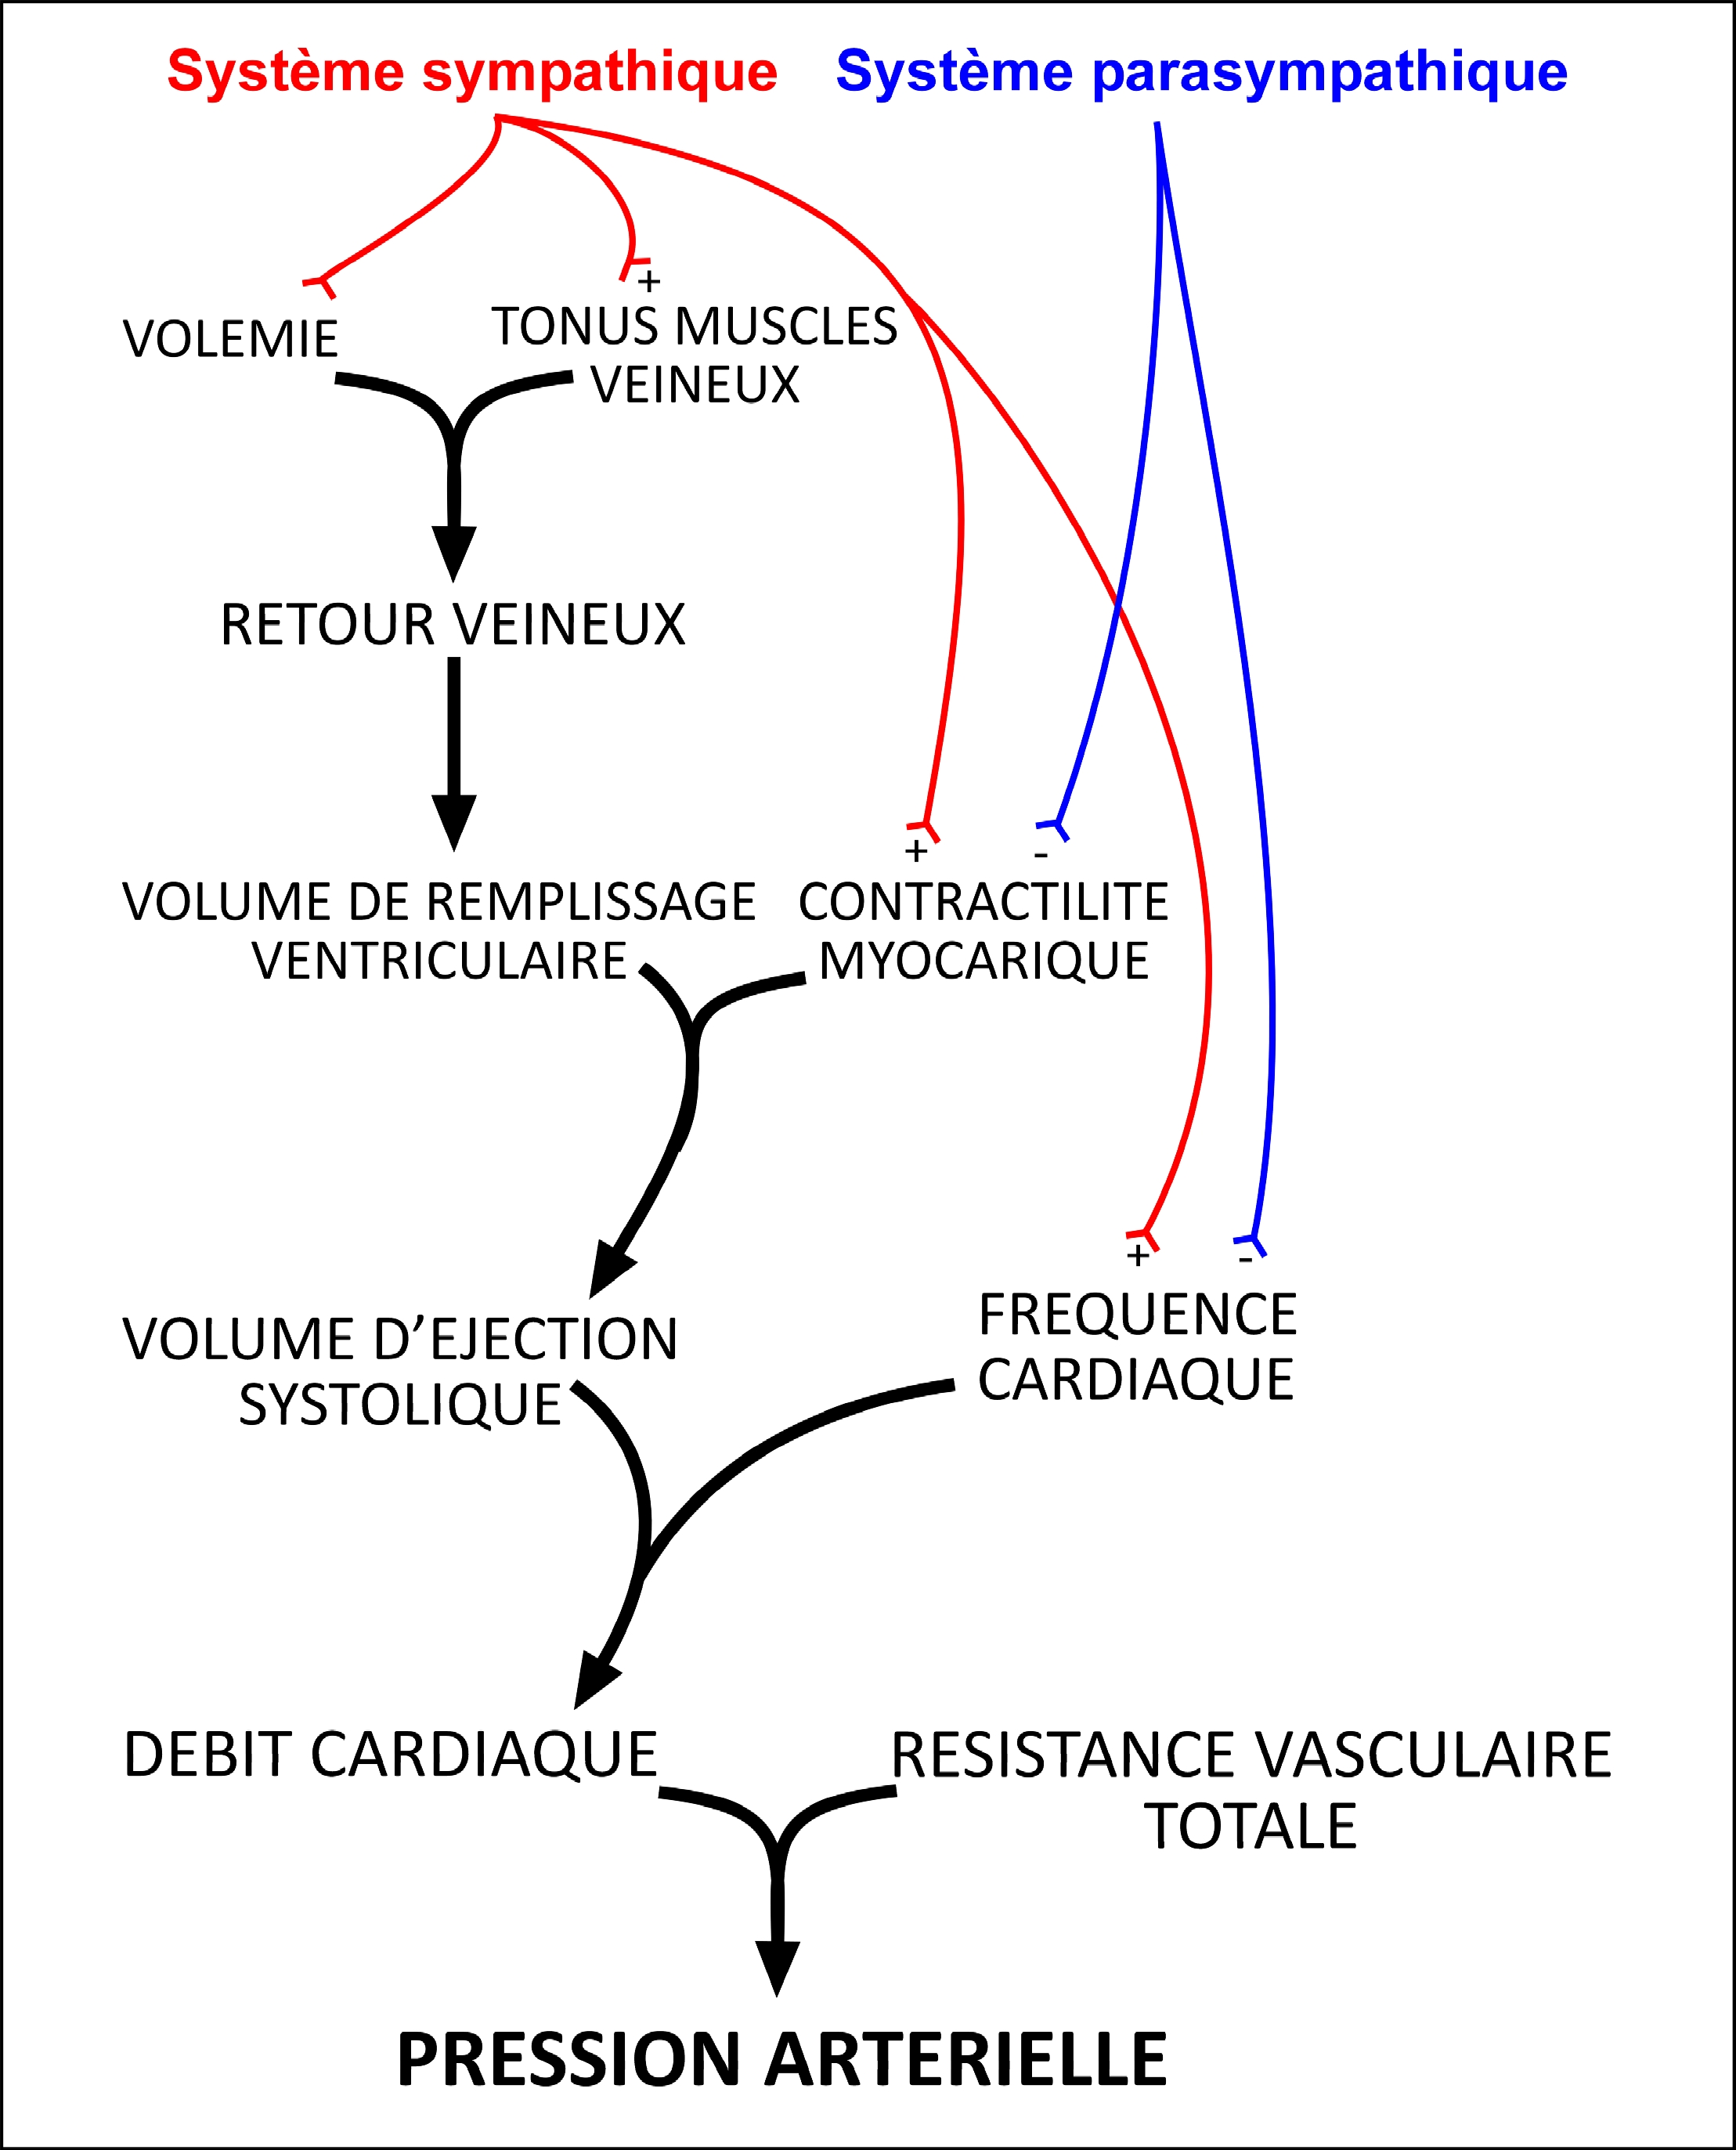
\includegraphics[scale=0.5]{Figure6.jpg} 
\end{center}

\caption[Facteurs déterminants de la pression artérielle et leur modulation par le système nerveux autonome]{\textbf{Facteurs déterminants de la pression artérielle et leur modulation par le système nerveux autonome}}

{\protect\parbox[t]{18cm}{
\begin{small}
Même si seules les régulations cardiaques sont détaillées dans ce manuscrit, on notera que le système nerveux autonome peut réguler la pression artérielle de manière plus indirecte. Seules les régulations influençant le débit cardiaque ont été représentées ici.
\end{small}}}

\label{Figure 6}

\end{figure}

\subsection{La résistance périphérique totale}

Cet élément, qui joue un rôle déterminant dans la régulation de la pression artérielle, correspond à la résistance que les parois vasculaires opposent à l’écoulement du sang. Le compartiment vasculaire total peut être schématiquement divisé en trois sous-compartiments ou réseaux : le réseau artériel, le réseau artériolaire et le réseau veineux, chacun étant caractérisé par une résistance locale. La résistance périphérique totale est la résultante de l’ensemble de ces résistances.

\begin{description}
\item [\textbullet~Le réseau artériel (depuis l’aorte jusqu’aux artérioles) est très ramifié.] La pression artérielle moyenne est maintenue dans des limites très étroites. Le débit et la pression y sont pulsatifs (conséquence directe du fonctionnement cyclique du cœur) et la résistance à l’écoulement est faible. Le volume de sang contenu dans le réseau artériel est faible comparé à celui présent dans le réseau veineux.
\item [\textbullet~Le réseau artériolaire (ou « réseau résistif »)] : la résistance à l’écoulement y est élevée et ajustable. Ce réseau est l’effecteur le plus efficace dans la régulation de la pression artérielle. Les sphincters artériolaires réduisent la pression à l’entrée des capillaires et y contrôlent en permanence le débit sanguin. 
\item [\textbullet~Le réseau veineux (ou « réseau capacitif »)] : la pression veineuse est faible ainsi que la résistance à l’écoulement. Les veines contiennent la plus grande partie du volume sanguin. La grande extensibilité de leurs parois permet de conserver un domaine de basse pression et cela malgré une importante variation du volume sanguin.
\end{description}

La résistance périphérique totale est modulée, non seulement, par le système nerveux autonome mais aussi par un mécanisme de régulation locale indépendant de celui-ci qui contrôle le flux sanguin au niveau de chaque organe. Cette régulation permet de conserver un débit sanguin local constant malgré de larges variations de la pression artérielle systémique. Elle permet aussi d’ajuster le flux sanguin en fonction des besoins énergétiques locaux. Ainsi, toute augmentation de l’activité métabolique locale s’accompagne d’une vasodilatation, et à l’inverse, la réduction des besoins énergétiques induit une vasoconstriction. Cette régulation dépend directement du pH, des pO$_{2}$ et pCO$_{2}$ et de la concentration locale d’acide lactique. Ces différents facteurs ont la propriété de provoquer l’ouverture des sphincters pré-capillaires et d’augmenter le diamètre des artérioles, et donc d’accroître localement le flux sanguin.

\subsection{Contrôle par le système nerveux autonome sympathique}

\subsubsection{Au niveau périphérique}

Les neurones préganglionnaires sympathiques sont localisés dans la corne intermédiolatérale de la moelle épinière. Ces neurones envoient des projections cholinergiques (courtes) aux ganglions sympathiques localisés de chaque côté de la moelle et à la glande médullosurrénale. Les neurones des ganglions sympathiques envoient à leur tour des projections postganglionnaires noradrénergiques (longues) sur leurs organes cibles.

La noradrénaline libérée par ces projections a :

\begin{itemize}
\item au niveau du cœur, des effets chronotrope et inotrope positifs, via l’activation de récepteurs $\beta_{1}$ et $\beta_{2}$ adrénergiques, 
\item au niveau des vaisseaux, un effet vasoconstricteur par stimulation de récepteurs $\alpha_{1}$ adrénergiques (voir Figure 7).
\end{itemize}

La fréquence de décharge des cellules pré- et post-ganglionnaires sympathiques détermine le tonus sympathique, donc la libération de noradrénaline au niveau des organes cibles, et in fine, la valeur de la pression artérielle. Il est admis que dans les conditions physiologiques (pression artérielle moyenne de l’ordre de 100 mmHg chez le rat), les cellules préganglionnaires sympathiques (et, par conséquent, les cellules ganglionnaires) déchargent de manière tonique.

\subsubsection{Rôle central de la région rostroventrolatérale du bulbe}

Les cellules préganglionnaires sympathiques ne déchargent pas en absence d’influx nerveux. Elles sont dépourvues d’activité intrinsèque de type pacemaker (Guyenet 1990) : leur décharge tonique est dépendante d’impulsions excitatrices. Ces impulsions proviennent en grande majorité de la région rostroventrolatérale du bulbe (RVL), située caudalement par rapport au noyau facial (voir Figure \ref{Figure 7} B2 - page \pageref{Figure 7}). Plusieurs études anatomiques montrent qu’il existe effectivement des projections de la RVL vers la corne intermédiolatérale (Loewy et al. 1981; Ross et al. 1984a; Tucker et al. 1987; Milner et al. 1988). De plus, cette région, qui contient des neurones « sympathoexcitateurs » assurant le tonus sympathique basal, est considérée comme un véritable centre presseur (Guertzenstein \& Silver 1974; Spyer 1981; Willette et al. 1984; Sun \& Guyenet 1986; Sun et al. 1988).

Des expériences de micro-stimulation ont montré qu’en fonction du site de la RVL stimulé différents patterns d’activités des nerfs sympathiques pouvaient être évoqués. Ces expériences ont amené à émettre l’hypothèse d’une organisation « organotopique » de ces neurones sympathoexcitateurs. Des sous-groupes de neurones individualisés seraient préférentiellement dédiés au contrôle de certains organes (McAllen \& Dampney 1990; McAllen et al. 1995; Campos \& McAllen 1997). Toutefois les études anatomiques utilisant des virus neurotropes comme traceur transneuronal et montrant un haut degré de « collatéralisation » de ces neurones, remettent en question une telle hypothèse (Jansen et al. 1995; Sved et al. 2001; Kerman et al. 2003; Stornetta et al. 2004).

\begin{figure}[p]

\begin{center}
 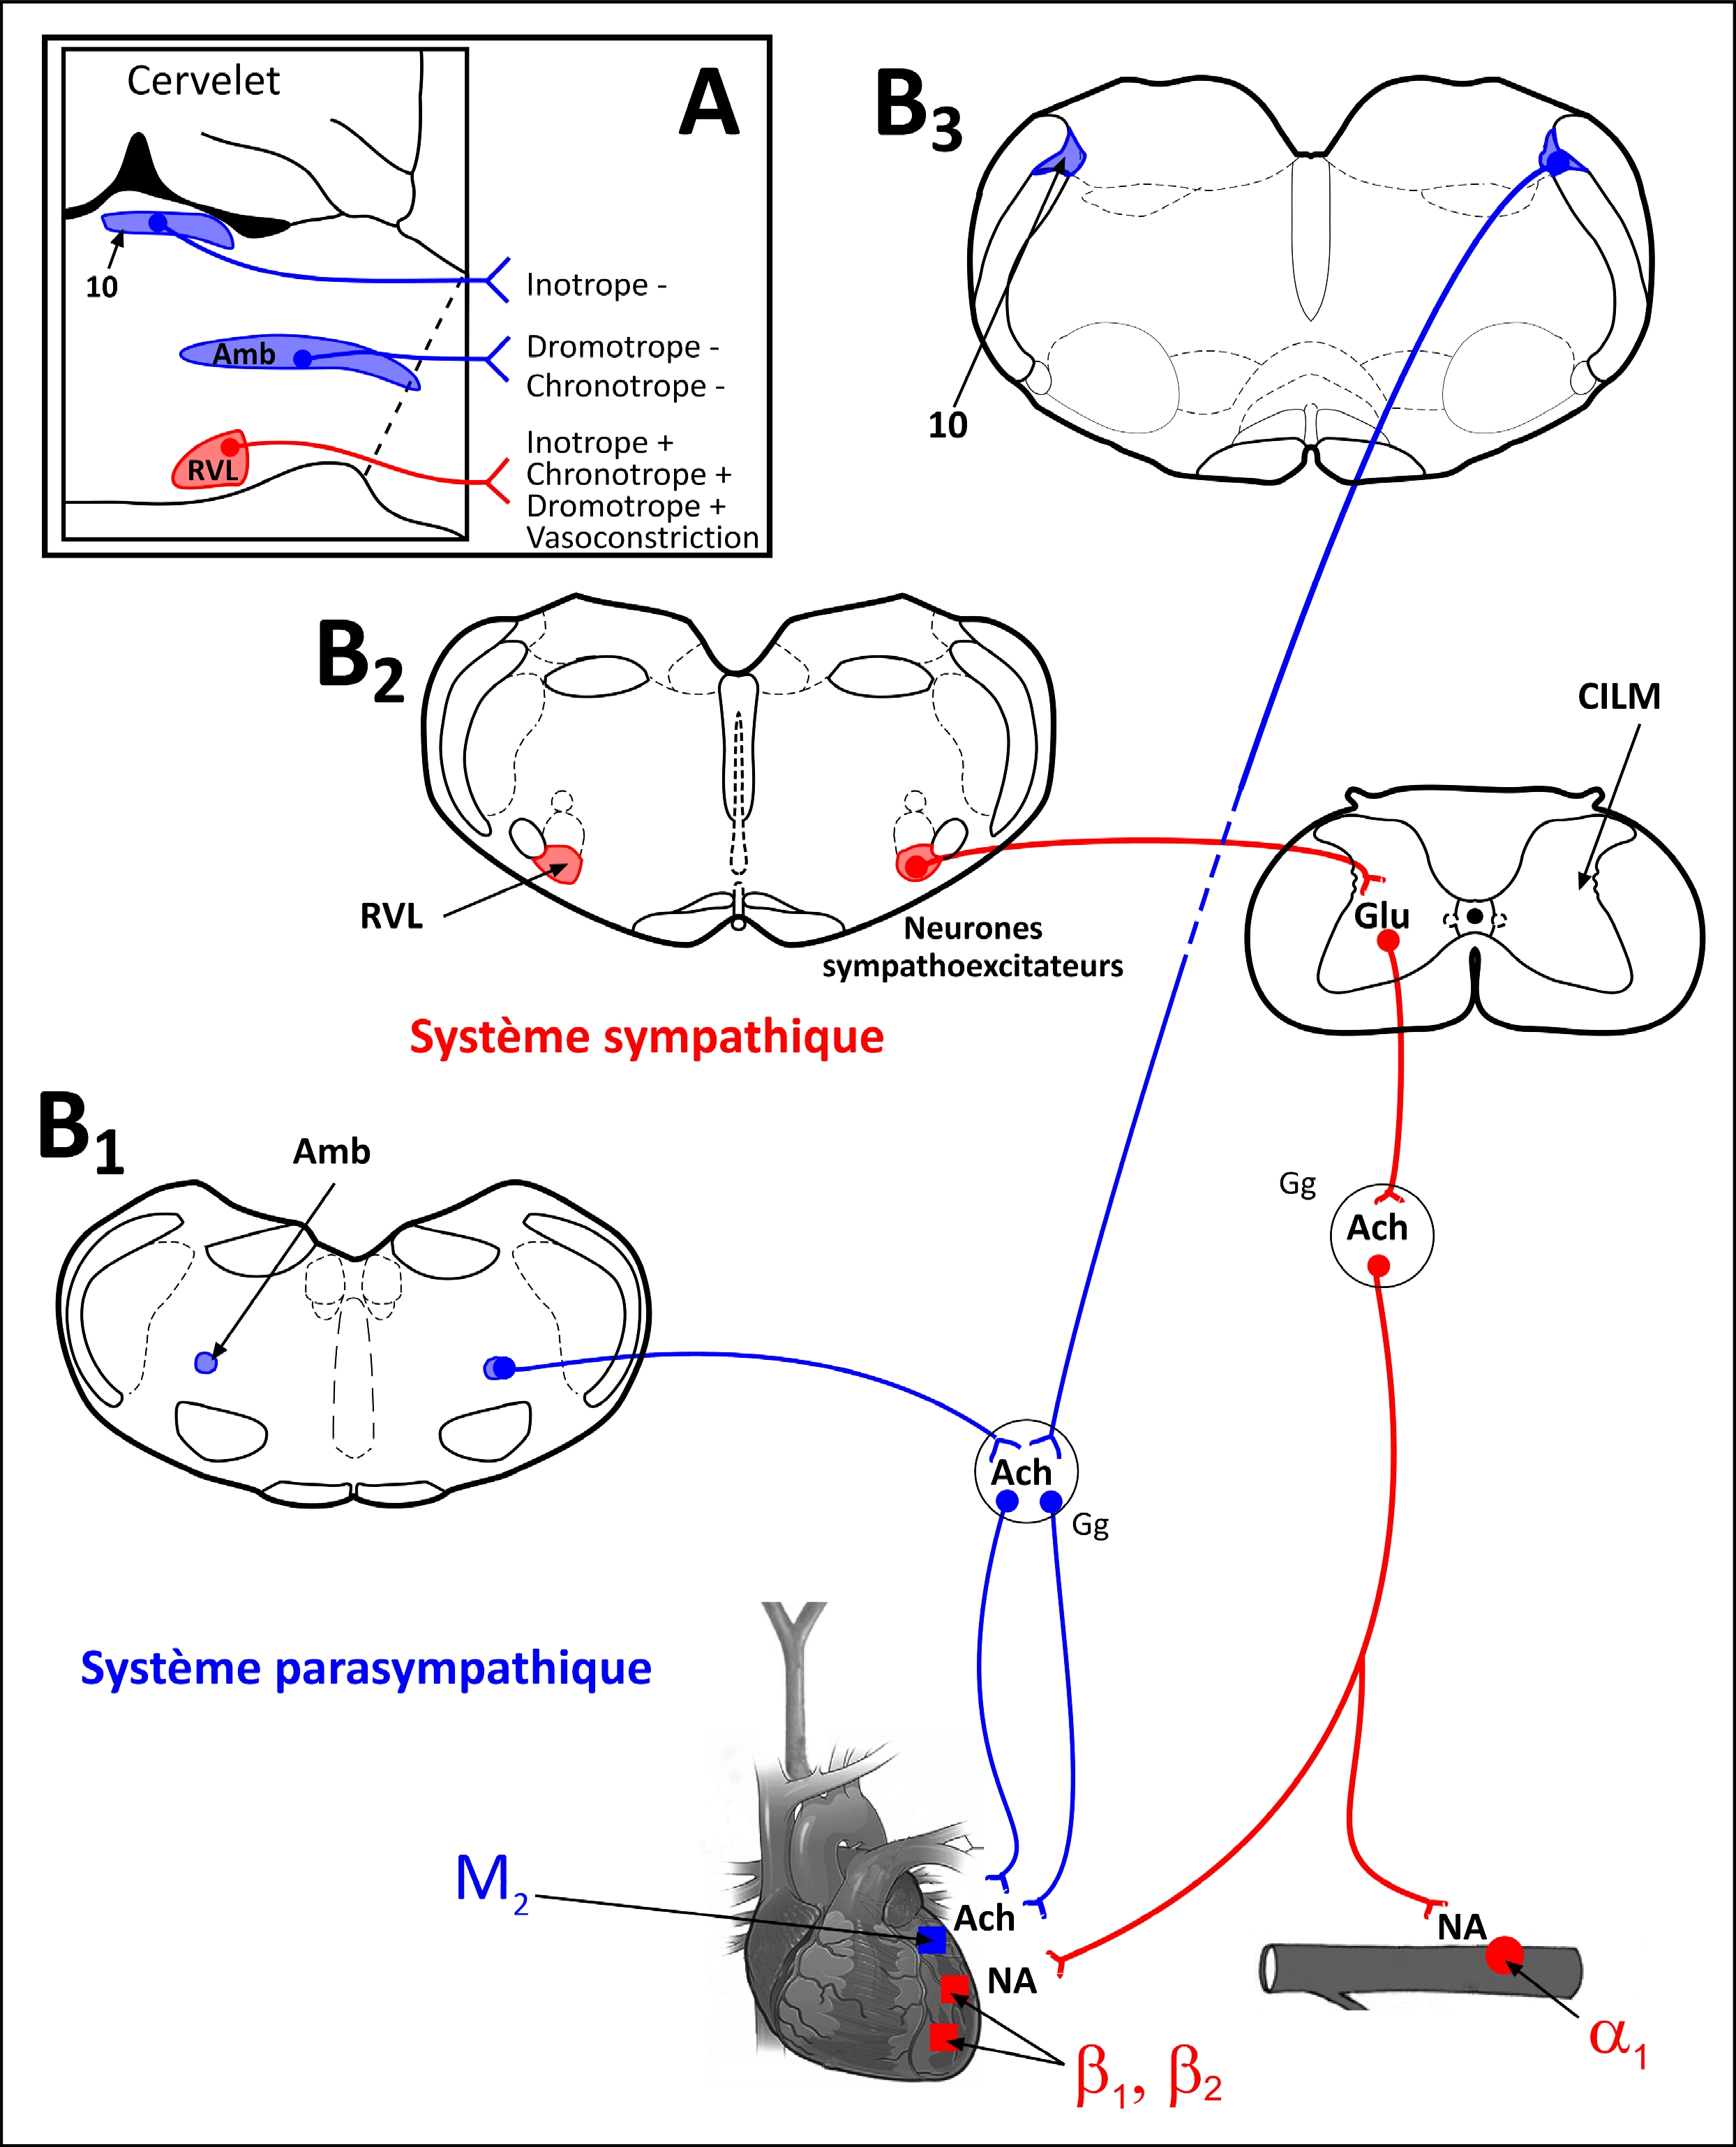
\includegraphics[width=18cm]{Figure7.jpg} 
\end{center}

\caption{\textbf{Contrôle de la pression artérielle par le système nerveux autonome}}

{\protect\parbox[t]{18cm}{
\begin{small}
\center{\textit{\textbf{Influences sympathiques et parasympathiques sur le cœur et les vaisseaux}}}\\
B1 : -13,00 mm ; B2 : -12,12 mm ; B3 : -11,52 mm postérieur à bregma ; $\alpha$ : Récepteurs alpha adrénergiques ; $\beta$ : Récepteurs béta adrénergiques ; Ach : Acétylcholine ; CILM : Corne intermédiolatérale de la moelle épinière ; Gg : Ganglion ; M$_{2}$ : Récepteurs muscariniques ; NA : Noradrénaline ; Amb : Noyau Ambigu ; 10 : Noyau dorsal du nerf vague ; RVL : région rostroventrolatérale du bulbe
\end{small}}}

\label{Figure 7}

\end{figure}

Les neurones sympathoexcitateurs de la RVL répondent aux critères définis par Brown et Guyenet (Brown \& Guyenet 1985) : 

\begin{itemize}
\item ils sont activés par une stimulation antidromique au niveau de la corne intermédiolatérale de la moelle épinière,
\item ils déchargent de manière synchrone à l’onde de pression,
\item ils sont barosensibles, c’est-à-dire inhibés lors de l’activation du baroréflexe
\footnote{Il faut toutefois noter l’existence d’efférences sympathoexcitatrices affectant le système cardiovasculaire et sensibles à des variations de température ou de glycémie. Mais ces efférences n’affectent pas directement le cœur et ne jouent qu’un rôle secondaire dans le contrôle de la pression artérielle (Guyenet 2006).}.
\end{itemize}

Ceci dit, les neurones sympathoexcitateurs de la RVL reçoivent et intègrent des messages en provenance de structures centrales et de récepteurs périphériques, dont les barorécepteurs (Granata et al. 1983; Ross et al. 1984a; Ross et al. 1984b). 

Ces neurones sympathoexcitateurs ne constituent pas une population cellulaire homogène. Ils peuvent être classés en trois populations en fonction : de leur sensibilité à la clonidine (agoniste mixte des récepteurs $\alpha$2 adrénergiques et imidazoliques), de leur vitesse de conduction, et de leur rythme de décharge à des pressions artérielles basses (70 mmHg) (Sun \& Guyenet 1986; Sevoz-Couche et al. 1998). Seule une fraction de ces neurones (les neurones clonidine-insensibles et à vitesse de conduction faible) semblent décharger de façon tonique in vitro, en absence de tout influx nerveux (Sun et al. 1988). Cette activité pacemaker intrinsèque fait de ce groupe de neurones un bon candidat comme source de l’influence sympathique tonique. Mais cette hypothèse, émise par Guyenet et al. (1985), n’a toujours pas été confirmée \textit{in-vivo} (Brown \& Guyenet 1985).

Le principal neurotransmetteur libéré au niveau de la corne intermédiolatérale par les afférences en provenance des neurones sympathoexcitateurs de la RVL semble être le glutamate (voir Figure \ref{Figure 7} - page \pageref{Figure 7}). Cette hypothèse, proposée par Morrisson et al. (1991), a été confirmée par Deuchars et al. (1995). Ces auteurs ont montré que les deux composantes des PPSE évoqués, au niveau des neurones préganglionnaires sympathiques de la corne intermédiolatérale, par une stimulation de la RVL étaient éliminées par l’administration d’antagonistes des récepteurs ionotropiques du glutamate (Morrison et al. 1991; Deuchars et al. 1995). Toutefois, un rôle des catécholamines dans cette neurotransmission n’est pas complètement exclu. En effet, la moitié des cellules adrénergiques de la RVL projettent sur la corne intermédiolatérale (Tucker et al. 1987; Milner et al. 1988) et une partie des cellules glutamatergiques de la RVL exprime l’enzyme catalysant l’étape limitante de la voie de synthèse de l’adrénaline (Nosjean et al. 2002).

\subsubsection{Rôle secondaire de la région rostroventromédiane du bulbe}

Les noyaux raphé bulbaires et la RVM contiennent aussi des neurones sympathoexcitateurs (McCall \& Clement 1989). En effet, la RVM projette dans les cornes intermédiolatérales sur les neurones sympathiques préganglionnaires et les motoneurones dans la moelle épinière (voir « \ref{Projections de la RVM} Projections de la région rostroventromédiane du bulbe » - page \pageref{Projections de la RVM} et « \ref{Afférences, proj, transmission} Afférences, projections et transmission synaptique » - page \pageref{Afférences, proj, transmission}). En accord avec cette donnée anatomique, les études utilisant des virus neurotropes comme traceur transneuronal ont montré que les neurones sérotoninergiques et non-sérotoninergiques de la RVM était connectés de façon oligosynaptique à de nombreuses cibles du système nerveux autonome (Mason 2001; Cano et al. 2003; Toth et al. 2006).

Plusieurs études récentes ont montré que ces cellules étaient probablement impliquées dans la régulation de la circulation cutanée (Blessing et al. 1999; Blessing \& Nalivaiko 2001), notamment, après des stimuli nociceptifs (Nalivaiko \& Blessing 1999) ou lors de situations de stress intense (Vianna et al. 2008). Il semblerait aussi que les neurones sympathoexcitateurs de cette région soient impliqués dans la tachycardie induite pendant un stress intense (Zaretsky et al. 2003a; Zaretsky et al. 2003b; Vianna et al. 2008).

La sérotonine de la RVM semble jouer un rôle très important à ce niveau. En effet au niveau spinal, elle dépolarise les neurones sympathiques préganglionnaires et sa libération est importante pour le maintien du tonus sympathique et de la pression artérielle (Coote et al. 1981; Kadzielawa 1983; Lewis \& Coote 1990).

\subsection{Contrôle par le système nerveux autonome parasympathique}

Le système nerveux parasympathique participe à la régulation de la pression artérielle par l’intermédiaire du contrôle de la fréquence et de la contractilité cardiaques.

Les neurones préganglionnaires parasympathiques bulbaires envoient des projections cholinergiques (longues), via le nerf vague, sur les cellules ganglionnaires situées contre ou à l’intérieur de l’organe cible. Ces cellules ganglionnaires envoient à leur tour des projections cholinergiques (courtes) vers les cellules cibles du myocarde. L’excitation des cellules ganglionnaires provoque la libération d’acétylcholine, qui vient activer des récepteurs muscariniques M$_{2}$, entraînant une bradycardie (effet chronotrope négatif) et une réduction de la contractilité (effet inotrope négatif) (voir Figure \ref{Figure 7} - page \pageref{Figure 7}). Si l’on bloque ces récepteurs muscariniques, par une administration systémique d’atropine, le tonus parasympathique est totalement inhibé. On observe alors une tachycardie révélant qu’il existe, en temps normal, une influence tonique du système parasympathique sur le cœur. Cette influence résulte en majeure partie de l’activité tonique des barorécepteurs périphériques (voir ci dessous). 

La localisation bulbaire des neurones préganglionnaires parasympathiques reste un sujet très discuté, malgré les nombreuses études qui lui ont été consacrées. Il est généralement admis que ces neurones sont localisés dans le noyau ambigu (voir Figure \ref{Figure 7} B1 - page \pageref{Figure 7})(Stuesse 1982; Izzo et al. 1993), ainsi que dans le noyau dorsal du vague (voir Figure \ref{Figure 7} B3 - page \pageref{Figure 7}) (Calaresu \& Pearce 1965; Ciriello \& Calaresu 1980). La fonction des neurones préganglionnaires parasympathiques dépendrait de leur origine. 

\begin{itemize}
\item Les neurones du noyau ambigu, envoyant au cœur des fibres myélinisées, auraient une influence sur le chronotropisme (voir Figure \ref{Figure 7} A - page \pageref{Figure 7}) (McAllen \& Spyer 1976; Geis et al. 1981; Jordan et al. 1982). 
\item Les neurones localisés dans le noyau dorsal du vague contrôleraient (via des fibres C non myélinisées) préférentiellement l’inotropisme cardiaque (voir Figure \ref{Figure 7} A - page \pageref{Figure 7}).
\end{itemize}

Ces derniers résultats ont été obtenus à la fois chez le rat (Jordan \& Spyer 1986), le chat et le chien (Geis et al. 1981). La relation entre l’origine et la fonction des neurones préganglionnaires parasympathiques est aujourd’hui clairement établie (Massari et al. 1995; Blinder et al. 1998).

Du point de vue neurochimique, on distingue différentes classes de neurones cardiaques préganglionnaires (Takanaga et al. 2003). Ainsi, dans les neurones cholinergiques du noyau du nerf vague, l’acétylcholine peut être colocalisée avec la NO synthase. De même, dans le noyau ambigu, certains neurones cholinergiques contiennent du CGRP. D’ailleurs, il semble exister une relation entre les caractéristiques neurochimiques des cellules préganglionnaires parasympathiques et leur activité fonctionnelle.

Ces voies sympathiques et parasympathiques peuvent être modulées pour ajuster rapidement les valeurs de la pression artérielle en fonction des différentes conditions physiologiques, et ceci par l’intermédiaire des réflexes cardiovasculaires.

\subsection{Les réflexes cardiovasculaires }
\label{Réflèxes cardiovasculaires}

Trois réflexes cardiovasculaires peuvent affecter la pression artérielle à court terme : le baroréflexe, le chémoréflexe cardiopulmonaire (ou réflexe de Bezold-Jarisch) et le chémoréflexe carotidien. Ils sont tous les trois caractérisés par une réponse sympathique et une réponse parasympathique. Si la réponse sympathique diffère selon les réflexes, ils ont en revanche la même réponse parasympathique. Celle-ci aboutit à une diminution de la fréquence cardiaque. 

Lors de ma thèse, je me suis principalement intéressé au baroréflexe. Dans les pages suivantes, je me contenterai donc de décrire les circuits neuronaux sous-tendant son fonctionnement. 

\subsubsection{Le baroréflexe}

Le baroréflexe est un rétrocontrôle réflexe indispensable à la survie de l’organisme, car il joue un rôle déterminant dans l’homéostasie cardiovasculaire. En effet, toute élévation de la pression artérielle au-delà d’une valeur seuil active les barorécepteurs, situés au niveau de la crosse aortique et du sinus carotidien, et déclenche instantanément un ajustement compensatoire : 

\begin{itemize}
\item une bradycardie par excitation vagale (composante parasympathique du baroréflexe
\footnote{Les travaux de cette thèse étant focalisés sur cette composante, il est bon de préciser que les termes : composante parasympathique du baroréflexe, composante cardiaque ou cardiovagale du baroréflexe, baroréflexe cardiovagal, bradycardie réflexe seront utilisés de manière synonyme dans la suite de ce manuscrit.}
) et inhibition sympathique, et
\item une vasodilatation par inhibition sympathique (composante sympathique du baroréflexe) (voir Figure \ref{Figure 8} - page \pageref{Figure 8}).
\end{itemize}

La bradycardie et la vasodilatation se traduisent par une diminution de la pression artérielle permettant de compenser l’élévation initiale. Une diminution de la pression artérielle aura naturellement l'effet opposé. 

Comme les valeurs physiologiques normales de la pression artérielle systolique dépassent la valeur seuil d’activation des barorécepteurs, le baroréflexe exerce donc, en permanence, un tonus vagal cardiomodérateur et une inhibition du tonus sympathique vasomoteur. En conséquence, la dénervation totale des afférences baroréceptrices élève la pression artérielle (hypertension neurogénique) et la rend plus instable (Krieger 1964; Norman et al. 1981). Cependant, à long terme, la pression artérielle revient progressivement à son niveau initial et seule persiste sa variabilité accrue (Norman et al. 1980). Ainsi, le baroréflexe exerce, à court terme, un contrôle tonique du niveau de la pression artérielle, mais, à long terme, il intervient plutôt pour assurer sa stabilité.

Chez l’animal, le baroréflexe peut être expérimentalement déclenché de différentes façons : 

\begin{itemize}
\item par stimulation électrique du nerf aortique dépresseur mais, dans ce cas, seules les afférences des barorécepteurs aortiques sont activées ;
\item en provoquant une hypertension suffisante pour activer les barorécepteurs aortiques et carotidiens par administration d’un agent vasoconstricteur comme la phényléphrine. Cette molécule active directement les récepteurs $\alpha$1 adrénergiques situés à l’intérieur des vaisseaux, déclenche une vasoconstriction généralisée et donc une augmentation intense et transitoire de la pression artérielle ;
\item en provoquant une hypertension mécaniquement par le gonflement d’un manchon placé autour de l’aorte abdominale. \end{itemize}

\subsubsection{Voies neuronales et structures impliquées dans le baroréflexe}

Les barorécepteurs carotidiens et aortiques sont des terminaisons nerveuses différenciées, localisées dans les parois des vaisseaux. L’étirement des parois provoqué par une augmentation de la pression et déclenche l’activation des barorécepteurs. Les corps cellulaires des afférences barosensibles aortiques et sinocarotidiennes sont respectivement localisés dans le ganglion plexiforme et dans le ganglion pétreux.

Il s’agit, en fait, de cellules pseudo-unipolaires (voir « \ref{Nocicepteurs : de la périphérie à la moelle} Les nocicepteurs : de la périphérie à la moelle épinière » - page \pageref{Nocicepteurs : de la périphérie à la moelle}), dont le soma se situe dans l’un ou l’autre de ces ganglions et dont les terminaisons des branches descendantes, ou périphériques, constituent les barorécepteurs. 

En provenance du ganglion plexiforme, la branche descendante se dirige vers la bifurcation aortique par l’intermédiaire du nerf de Cyon. La branche ascendante, ou centrale, constitue le nerf aortique dépresseur qui rejoint secondairement le nerf vague (X) (voir Figure \ref{Figure 8} B - page \pageref{Figure 8}).

De façon homologue, la branche descendante issue du ganglion pétreux se dirige vers le sinus carotidien par l’intermédiaire du nerf de Hering, alors que la branche ascendante est une composante du nerf glossopharyngien (IX) (voir Figure \ref{Figure 8} B - page \pageref{Figure 8}). 

Les branches ascendantes arrivent au niveau du noyau du tractus solitaire (NTS), une structure située dans la partie dorsale du bulbe (voir Figure \ref{Figure 8} B1 - page \pageref{Figure 8}) (Miura \& Reis 1972; Palkovits \& Zaborszky 1977; Kalia \& Mesulam 1980; Donoghue et al. 1981; Ciriello 1983). Des études électrophysiologiques ont mis en évidence l’activation de certains neurones du NTS à la suite d’une stimulation des afférences barosensibles (Mifflin et al. 1988). Le NTS est donc considéré comme le premier site central de projections des afférences des barorécepteurs. Il constitue le point de départ des composantes sympathique et parasympathique du baroréflexe. De fait, les lésions électrolytiques du NTS abolissent les réponses cardiovasculaires du baroréflexe (Lee et al. 1972). 

\begin{figure}[p]

\begin{center}
 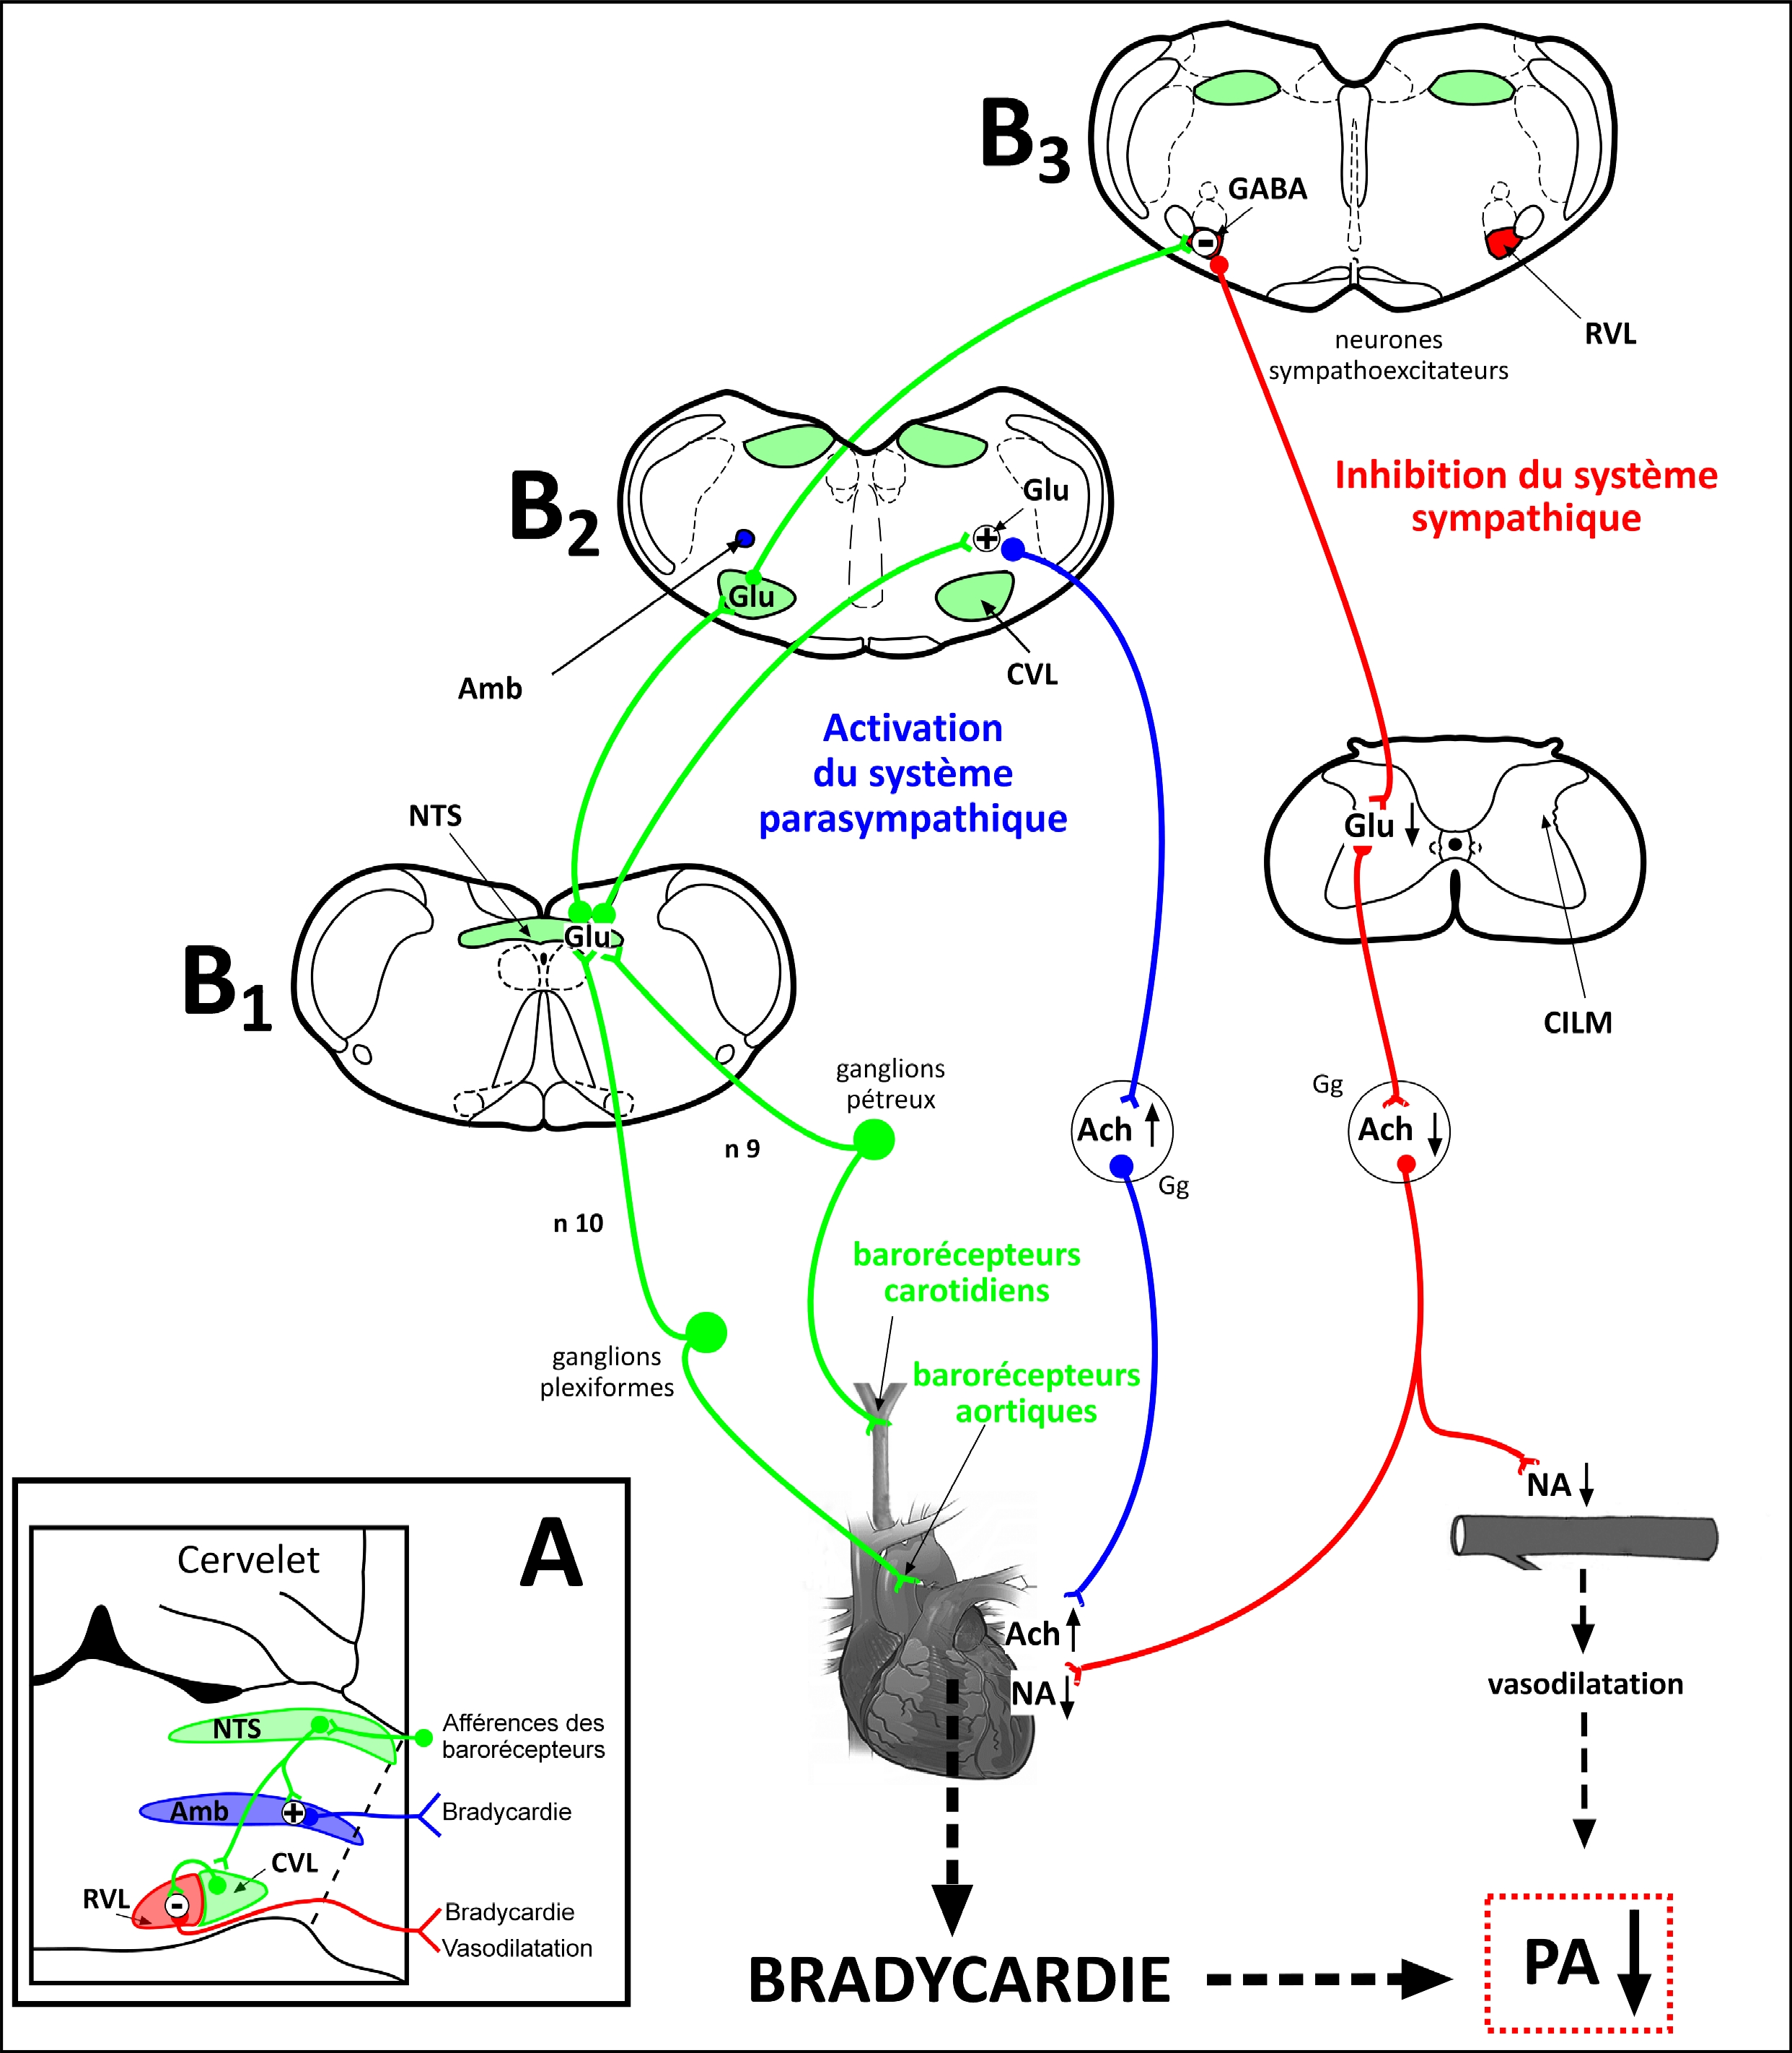
\includegraphics[width=18cm]{Figure8.jpg} 
\end{center}

\caption{\textbf{Le circuit du baroréflexe}}

{\protect\parbox[t]{18cm}{
\begin{small}
\center{\textit{\textbf{Schéma récapitulatif des voies bulbaires du baroréflexe}}}\\
B1 : -14,00 mm ; B2 : -13,00 mm ; B3 : -12,12 mm postérieur à Bregma ; n 9 : nerf glossopharyngien ; n 10 : nerf, Ach : Acétylcholine ; CILM : Corne intermédiolatérale de la moelle épinière ; CVL : région caudoventrolatérale du bulbe ; GABA : acide gamma-amino-butyrique ; Gg : Ganglion ; Glu : glutamate ; NA : Noradrénaline ; Amb : Noyau Ambigu ; NTS : noyau du tractus solitaire ; RVL : région rostroventrolatérale du bulbe
\end{small}}}

\label{Figure 8}

\end{figure}

\paragraph{Composante parasympathique du baroréflexe}

Les neurones du NTS impliqués dans cette composante projettent sur la partie la plus caudale du noyau ambigu, appelée noyau rétroambigu (voir Figure \ref{Figure 8} - page \pageref{Figure 8}). C’est dans cette région qu’est localisée la majorité des neurones préganglionnaires parasympathiques à destination du cœur (McAllen \& Spyer 1978; Spyer 1994). Ces projections semblent être glutamatergiques car la microinjection d’acide kynurénique, un antagoniste des récepteurs ionotropiques du glutamate, dans le noyau rétroambigu élimine la composante parasympathique du baroréflexe (Guyenet et al. 1987). D’ailleurs, les récepteurs NMDA et non-NMDA sont impliqués dans l’activation du noyau rétroambigu par les afférences issues du NTS (Neff et al. 1998).

\paragraph{Composante sympathique du baroréflexe}

La composante sympathique du baroréflexe correspond en réalité à une inhibition des neurones sympathoexcitateurs de la RVL, avec comme conséquence une vasodilatation et une bradycardie modérées. Les afférences excitatrices provenant des barorécepteurs activent, au niveau du NTS, des neurones glutamatergiques projetant sur la partie rostrale de la région caudoventrolatérale du bulbe (CVL) (Ross et al. 1985; Aicher et al. 1995). La libération de glutamate dans cette région, active des neurones GABAergiques qui projettent sur les neurones sympathoexcitateurs de la RVL (Minson et al. 1997; Chan \& Sawchenko 1998) (voir Figure \ref{Figure 8} - page \pageref{Figure 8}). 

Ainsi, la composante sympathique du baroréflexe peut être bloquée par :

\begin{itemize}
\item l’injection dans la CVL d’un antagoniste des récepteurs ionotropiques du glutamate (l’acide kynurénique) (Guyenet et al. 1987),
\item l’injection dans la RVL d’un antagoniste des récepteurs GABA$_{A}$ (Verberne \& Guyenet 1992).
\end{itemize}

Comme nous le verrons dans la partie suivante, le baroréflexe est modulé dans certaines circonstances. Ces modulations se font au niveau du NTS, très tôt dans l’arc du baroréflexe. Cette structure et son organisation interne jouent donc un rôle essentiel dans ces modulations.

\section{Anatomie du noyau du tractus solitaire}

Le NTS est un centre d’intégration des différentes régulations végétatives et de la sensibilité viscérale non consciente. Ainsi, il participe à la régulation de la respiration (Kalia et al. 1979), de la fonction gastrointestinale (Sevoz et al. 1996b), de la sécrétion hormonale, comme par exemple celle de la vasopressine (Day \& Sibbald 1989; Raby \& Renaud 1989), du cycle veille-sommeil (Nosjean et al., 1987) et de la nociception (Lewis et al. 1987; Sevoz-Couche et al. 2002a). Enfin, le NTS joue aussi un rôle clé dans la régulation réflexe de la pression artérielle via le traitement des messages qu’il reçoit directement des barorécepteurs. 

Au plan anatomique, le NTS est une structure située dans la région dorsomédiane du bulbe (voir Figure \ref{Figure 9} - page \pageref{Figure 9}). Il encadre l’area postrema et le 4\textsuperscript{ème} ventricule. Il s’étend rostro-caudalement du pôle caudal du noyau moteur du nerf facial à la décussation pyramidale (Torvik 1956; Kalia \& Sullivan 1982). Le NTS est subdivisé en 3 sous-noyaux : les NTS rostral, intermédiaire et caudal (ou commissural) (voir Figure \ref{Figure 9} - page \pageref{Figure 9}). Les deux sous-noyaux antérieurs sont eux-mêmes subdivisés en deux parties, médiane et latérale (Cottle 1964; Miura \& Reis 1972; Chiba \& Doba 1975). Ces sous-noyaux présentent des différences à la fois hodologiques et fonctionnelles.

Le NTS rostral (gustatif) est formé de deux colonnes cellulaires qui encadrent le 4\textsuperscript{ème} ventricule. Il s’étend du pôle caudal du noyau moteur du nerf facial au pôle rostral de l’area postrema. Sa partie latérale reçoit des afférences gustatives et somatiques des nerfs trijumeaux (V), faciaux (VII) et glossopharyngiens (Torvik 1956; Contreras et al. 1980). Il projette sur les noyaux des nerfs VII et XII (hypoglosse), mais aussi, pour une faible part, sur le noyau du nerf V (Loewy \& Burton 1978; Travers \& Norgren 1983). Il projette aussi de façon bilatérale sur les noyaux latéral et dorsal de l’hypothalamus (Ricardo \& Koh 1978; Ciriello \& Calaresu 1980).

Le NTS intermédiaire est également formé de deux colonnes cellulaires au niveau de l’area postrema. Sa partie médiane reçoit des afférences viscérales des organes digestifs via le nerf vague alors que sa partie latérale reçoit des afférences du nerf IX (Contreras et al. 1980).

Le NTS commissural (caudal) est un sous-noyau unique formé par la réunion des NTS intermédiaires droit et gauche, au niveau de la partie caudale de l’area postrema. De là, il s’étend caudalement jusqu’à la décussation pyramidale. Ce sous-noyau reçoit des afférences viscérales des systèmes digestif et respiratoire et du cœur via le nerf vague (Torvik 1956; Contreras et al. 1980; Simon \& Schramm 1984; Wyss \& Donovan 1984). 

Le NTS caudal et intermédiaire, qui nous intéresse ici, est donc le relais primaire des messages autonomes/végétatifs. Toutefois, il reçoit aussi des afférences centrales issues des noyaux du raphé (Thor \& Helke 1987; 1989) et des noyaux postérolatéral et paraventriculaire de l’hypothalamus postérolatéral (Ricardo \& Koh 1978). 

Le NTS a plusieurs catégories de projections. En premier lieu, a été identifiée une projection descendante majeure sur les neurones préganglionnaires parasympathiques, localisés dans le noyau moteur dorsal du vague, le noyau ambigu et les noyaux salivaires inférieur et supérieur (Loewy \& Burton 1978; Norgren 1978; Ricardo \& Koh 1978; Ross et al. 1985; Cunningham \& Sawchenko 1989; Herbert et al. 1990; Dobbins \& Feldman 1994). Dans cette même projection, un contingent plus restreint est destiné aux neurones préganglionnaires sympathiques de la corne intermédiolatérale (Loewy \& Burton 1978). En second lieu, le NTS projette sur de nombreuses régions réticulaires incluant la RVL rostrale et caudale. En troisième lieu, le NTS envoie des projections ascendantes, dont la première et plus importante atteint l’aire parabrachiale (Herbert et al. 1990). De plus, le NTS envoie des projections sur plusieurs noyaux de l’hypothalamus (paraventriculaire, dorsomédian, arqué et préoptique médian) et sur l’amygdale centrale (Ricardo \& Koh 1978; Ciriello \& Calaresu 1980). Enfin, le NTS projette aussi sur plusieurs noyaux moteurs au niveau bulbaire (Loewy \& Burton 1978; Travers \& Norgren 1983).

Au titre d'un intérêt plus particulier pour les études présentées ici, il faut souligner que les afférences en provenance des barorécepteurs périphériques projettent essentiellement sur le NTS intermédiaire et commissural. De plus, les connexions entre le NTS et les structures bulbaires préganglionnaires (en particulier le noyau ambigu) constituent le support anatomique des voies sous-tendant les composantes sympathique et parasympathique du baroréflexe.

\begin{figure}[t]

\begin{center}
 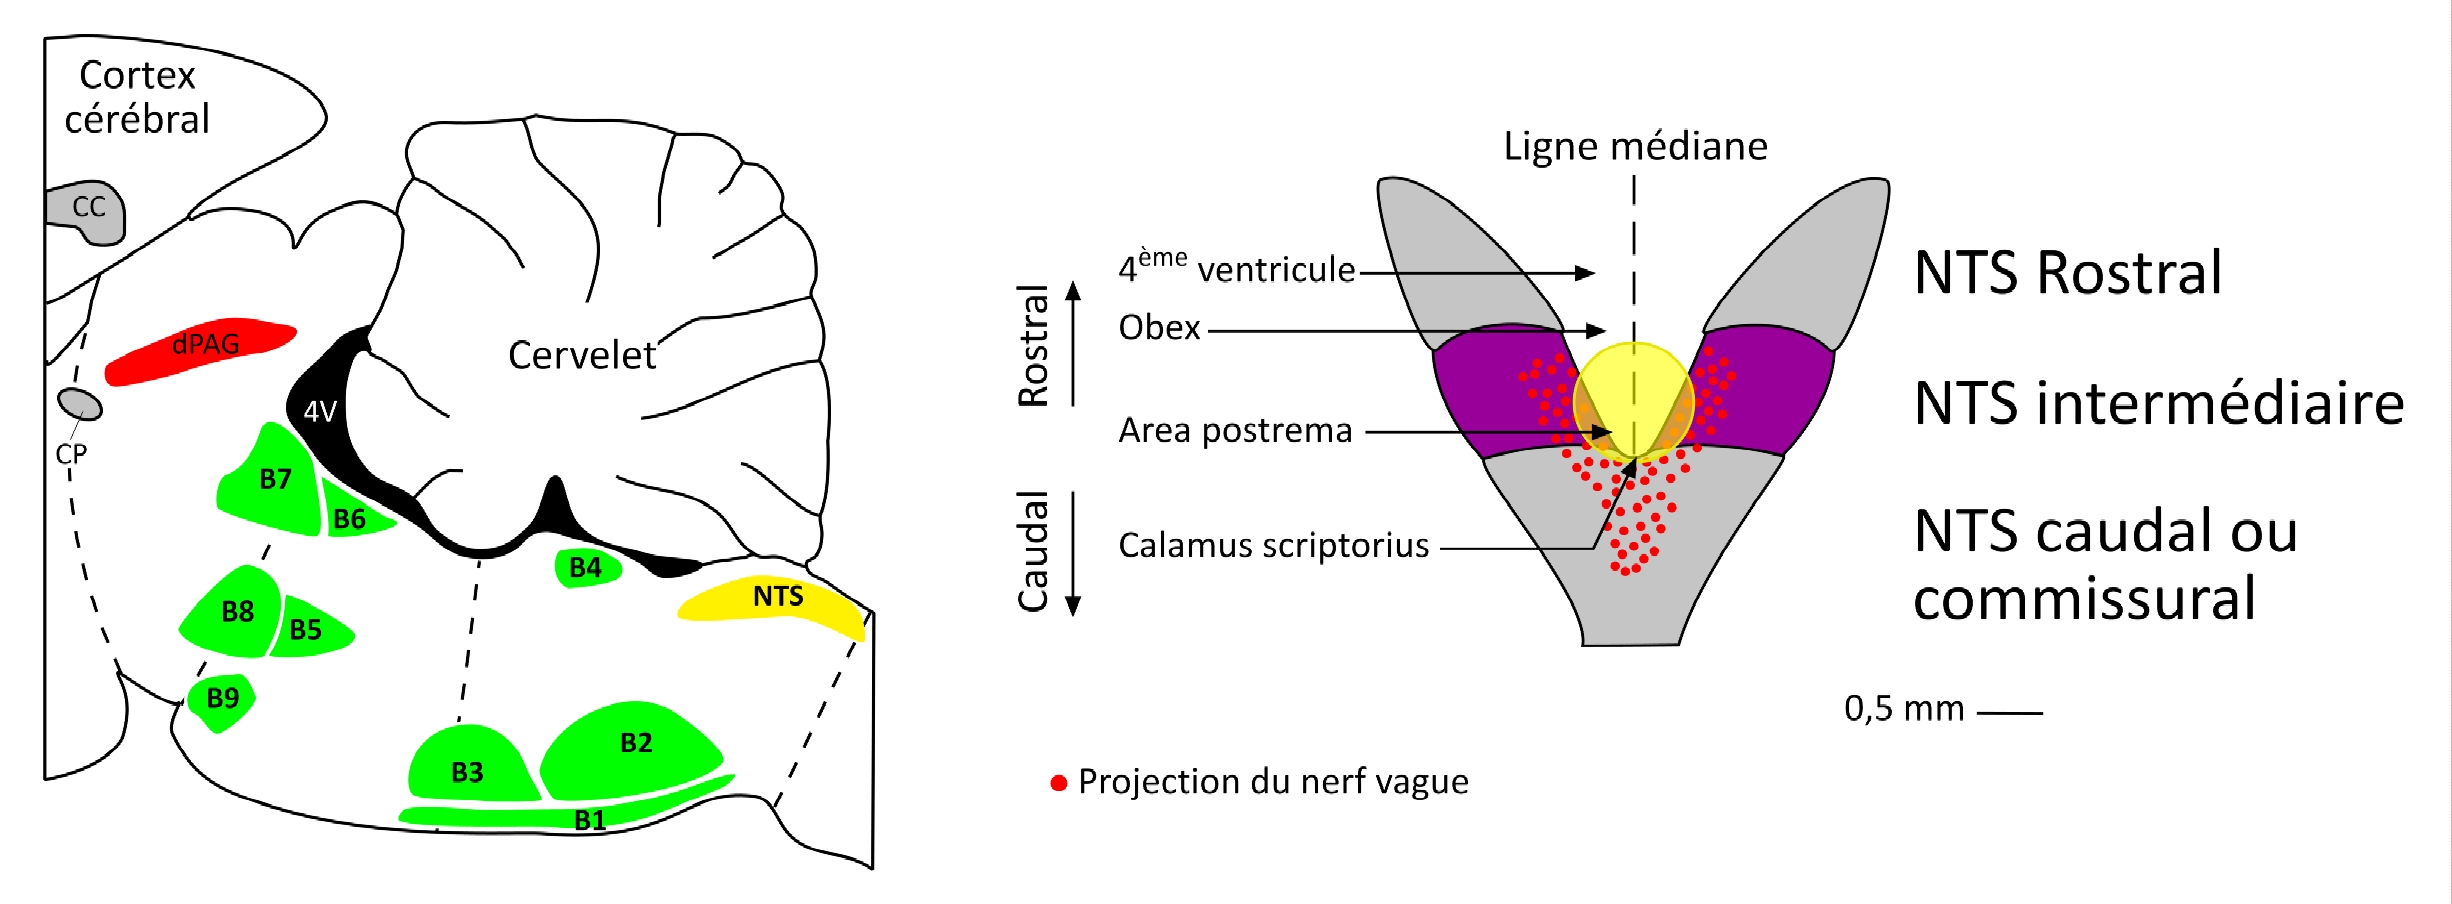
\includegraphics[width=18cm]{Figure9.jpg} 
\end{center}

\caption{\textbf{Le noyau du tractus solitaire}}

{\protect\parbox[t]{18cm}{
\begin{small}
\begin{center}
\textit{\textbf{Vue sagittale et dorsale du NTS avec ses divisions anatomiques et les principaux sites de projection des afférences vagales}}\end{center}
\end{small}}}

\label{Figure 9}

\end{figure}

\subsection{Neuromédiateurs du noyau du tractus solitaire et contrôle cardiovasculaire}

L’utilisation de techniques biochimiques, immunologiques et pharmacologiques a permis de montrer qu’une quarantaine de substances neuroactives, au moins, est présente dans cette structure (Palkovits \& Zaborszky 1977). Nombre de ces neuromédiateurs semblent impliqués dans la régulation de la pression artérielle. Dans ce mémoire, je me contenterai d’aborder les neuromédiateurs qui ont fait l’objet d’études approfondies dans la régulation du baroréflexe : le glutamate, le GABA, la sérotonine et la substance P.

\subsubsection{Le glutamate}

Le glutamate est le principal neurotransmetteur contenu dans les afférences vagales et glossopharyngiennes (Reis et al. 1981; Talman et al. 1981; Meeley et al. 1989). De fait, après vagotomie, le nombre de récepteurs glutamatergiques et le taux de glutamate dans le NTS diminuent (Dietrich et al. 1982; Lewis et al. 1988; Meeley et al. 1989). Par ailleurs, chez l’animal intact, la stimulation des afférences vagales entraîne la libération de glutamate au niveau du NTS (Granata \& Reis 1983). 

En fonction du site d’injection, la microinjection de glutamate dans le NTS entraîne des réponses différentes. Au niveau du NTS intermédiaire ou dans la partie latérale du NTS commissural, le glutamate provoque une hypotension et une bradycardie (Reis et al. 1981). En revanche, lorsque la microinjection de glutamate est faite au niveau de la partie médiane du NTS commissural, elle entraîne une hypertension (Colombari et al. 1994; Colombari et al. 1996).

La transmission des messages issus des afférences cardiovasculaires se fait principalement via des récepteurs ionotropiques (Guyenet et al. 1987; Vardhan et al. 1993b; 1993a; Zhang \& Mifflin 1993). Le débat reste toutefois ouvert sur l’importance relative des récepteurs NMDA et non-NMDA dans cette transmission (Kubo \& Kihara 1988; Gordon \& Leone 1991; Vardhan et al. 1993b; 1993a; Ohta \& Talman 1994; Haibara et al. 1995; Aylwin et al. 1997; Dean et al. 1998; Zhang \& Mifflin 1998; Machado et al. 2000; N'Diaye et al. 2001). Par ailleurs, la participation des récepteurs métabotropiques ne doit pas être écartée puisque, l’administration intra-NTS d’agonistes de ces récepteurs entraîne des réponses similaires à celles du baroréflexe (Machado \& Bonagamba 1998; Viard \& Sapru 2002). Cependant le blocage de ces récepteurs métabotropiques n’altère pas le baroréflexe (Antunes \& Machado 2003). 

\subsubsection{Le GABA}

L’innervation GABAergique du NTS est principalement d’origine intrinsèque. En effet, une densité importante de corps cellulaires GABAergiques a été mise en évidence dans les parties médiane, dorsale et commissurale du NTS (Dietrich et al. 1982; Meeley et al. 1985), ainsi que dans le NTS rostral (Lasiter \& Kachele 1988). 

La microinjection dans le NTS d’agonistes des récepteurs GABA provoque une élévation de la pression artérielle et une tachycardie (Bousquet et al. 1982; Sved \& Sved 1989; Florentino et al. 1990; Sved \& Sved 1990; Sved \& Tsukamoto 1992; Callera et al. 1999; 2000). Il a été suggéré que cet effet presseur, dépendant d’un mécanisme GABAergique, est la conséquence d’une inhibition de l’effet tonique cardiomodérateur du baroréflexe. En accord avec cette hypothèse, la stimulation des récepteurs GABAergiques du NTS supprime la bradycardie du baroréflexe aussi bien chez le rat anesthésié qu’éveillé (Bousquet et al. 1982; Sved \& Tsukamoto 1992; Okada \& Bunag 1995; Callera et al. 2000). De plus, les neurones du NTS, activés par la stimulation du nerf aortique dépresseur ou du nerf du sinus carotidien, sont inhibés par l’administration microiontophorétique de GABA (Mifflin et al. 1988). 

\subsubsection{La sérotonine}

Le rôle de la sérotonine, et en particulier des récepteurs 5-HT$_{3}$, dans la modulation du baroréflexe est au centre des travaux présentés dans cette thèse.
Le NTS présente une dense innervation sérotoninergique, essentiellement extrinsèque, d’origine centrale et périphérique (Fuxe 1965; Steinbusch 1981; Maley \& Elde 1982; Nosjean et al. 1987). La destruction des terminaisons sérotoninergiques du NTS par microinjection locale de 5,7-DHT entraîne, chez le rat vigile, une élévation de la pression artérielle qui dure plusieurs jours mais n’affecte ni la variabilité de la pression artérielle, ni la fréquence cardiaque (Orer et al. 1991).

Les afférences sérotoninergiques d'origine centrale proviennent de plusieurs des noyaux du raphé : magnus, pallidus, obscurus et, dans une moindre mesure, pontis et dorsal (Thor \& Helke 1987; Schaffar et al. 1988). 

Les afférences sérotoninergiques périphériques du NTS ont pour origine le ganglion plexiforme, où sont localisés les somas des neurones de premier ordre du baroréflexe aortique. L’existence d’une voie sérotoninergique ganglion plexiforme-NTS a été mise en évidence d’abord chez le chat (Gaudin-Chazal et al. 1983), puis chez le rat (Nosjean et al. 1990). La destruction spécifique des neurones sérotoninergiques du ganglion plexiforme (par microinjection locale de 5,7-DHT) a un effet similaire à celui de la dénervation spécifique des barorécepteurs. Elle provoque une hypertension transitoire accompagnée d’une augmentation durable de la variabilité de la pression artérielle (Norman et al. 1981; Orer et al. 1991). Ces afférences sérotoninergiques, issues du ganglion plexiforme, pourraient être responsables d’une partie des \textit{inputs} du baroréflexe aortique. Cette suggestion est aussi supportée par le fait que l’activation des barorécepteurs provoque la libération de sérotonine dans le NTS, et que cette libération est supprimée par la dénervation sino-aortique (Bhaskaran \& Freed 1988). 

La microinjection de sérotonine dans le NTS provoque des effets cardiovasculaires qui varient en fonction de la dose administrée, probablement via l’activation de différents récepteurs.

\begin{description}
\item [\textbullet~\`A des doses picomolaires], elle donne une hypotension et une bradycardie (Laguzzi et al. 1984; Merahi et al. 1992a), ainsi qu’une facilitation de la composante cardiovagale du baroréflexe (N'Diaye et al. 2001). 
\item [\textbullet~\`A des doses nanomolaires], elle provoque au contraire une inhibition de cette composante (Merahi et al. 1992b), associée à une élévation dose-dépendante de la pression artérielle, mais sans affecter de manière significative la fréquence cardiaque (Wolf et al. 1981; Merahi et al. 1992b; Tsukamoto et al. 2000). 
\end{description}

Au niveau du NTS, de nombreuses études électrophysiologiques, pharmacologiques et immunohistochimiques, ont permis d'identifier une grande densité de récepteurs 5-HT$_{3}$ (Pratt \& Bowery 1989; Glaum et al. 1992; Merahi et al. 1992b; Sevoz et al. 1996a; Sevoz et al. 1996b), 5-HT$_{1}$ (Hoyer et al. 1986; Manaker \& Verderame 1990), 5-HT$_{2}$ (Pazos et al. 1985; Merahi et al. 1992a; Sevoz-Couche et al. 2000b; 2000a; Sevoz-Couche et al. 2000c; Huang \& Pickel 2002), 5-HT$_{4}$ (Edwards \& Paton 1999) et 5-HT$_{7}$ (Gustafson et al. 1996). 
Les résultats de quelques unes de ces études consacrées aux récepteurs 5-HT$_{3}$, 5-HT$_{1A}$, et 5-HT$_{2}$ sont brièvement rappelés dans les paragraphes ci-dessous.

\paragraph{Les récepteurs 5-HT$_{3}$}

Dans le système nerveux central, le NTS est la structure présentant la plus grande densité de récepteurs 5-HT$_{3}$ (Pratt et al. 1990; Laporte et al. 1992). La forte densité de ces récepteurs dans le NTS a été confirmée chez l’être humain (Ohuoha et al. 1994).

Les afférences du NTS provenant du ganglion plexiforme expriment les sous-unités 5-HT$_{3A}$ et 5-HT$_{3B}$ (Morales \& Wang 2002). L’ablation unilatérale de ce ganglion provoque la disparition de la presque totalité des récepteurs 5-HT$_{3}$ dans le NTS ipsilatéral (Pratt \& Bowery 1989; Merahi et al. 1992b) confirmant leur localisation présynaptique sur ces afférences. Ces afférences étant glutamatergiques, l’activation des récepteurs 5-HT$_{3}$ du NTS provoque localement une augmentation de la libération de glutamate (Ashworth-Preece et al. 1995). De même, l’activation des neurones du NTS recevant des afférences vagales, par des agonistes des récepteurs 5-HT$_{3}$, impliquent l’activation de récepteurs ionotropiques du glutamate (Jeggo et al. 2005).

La microinjection d'agonistes sélectifs des récepteurs 5-HT$_{3}$, ou de doses nanomolaires de sérotonine dans le NTS, provoque les mêmes réponses cardiovasculaires : une inhibition de la composante parasympathique du baroréflexe et une élévation de la pression artérielle (Merahi et al. 1992b). L’inhibition de la bradycardie du baroréflexe, a été observée aussi bien sous anesthésie (Merahi et al. 1992b) que chez le rat éveillé (Callera et al. 1997). Ces réponses sont prévenues par la microinjection préalable d’antagonistes spécifiques des récepteurs 5-HT$_{3}$, mais pas celle d’antagonistes des autres récepteurs sérotoninergiques (Merahi \& Laguzzi 1995; Callera et al. 1997; Sevoz et al. 1997; Nosjean et al. 1998; Sevoz-Couche et al. 1998; Bonagamba et al. 2000). Les deux effets, induits par l’activation des récepteurs 5-HT$_{3}$ du NTS, sont sous-tendus par deux circuits distincts : 

L’inhibition de la composante parasympathique du baroréflexe est levée par la microinjection intra-NTS préalable d’un antagoniste des récepteurs GABA $_{A}$, suggérant que cette inhibition implique un interneurone GABAergique (Merahi et al. 1992b).

L’élévation de pression artérielle résulte de l’activation, de récepteurs glutamatergiques ionotropiques et du NO, de neurones glutamatergiques du NTS, qui vont à leur tour stimuler des neurones sympathoexcitateurs clonidine-sensibles, mais non catécholaminergiques, de la RVL. Ce schéma est supporté par tout un faisceau d’arguments et de données. 

\underline{Au niveau du NTS :}

\begin{itemize}
\item La microinjection préalable d’antagonistes des récepteurs ionotropiques du glutamate dans le NTS prévient l’effet presseur provoqué par l’activation des récepteurs 5-HT$_{3}$ (Sevoz-Couche et al. 2002b).
\item Dans certains neurones du NTS, les récepteurs ionotropiques du glutamate coexistent avec la NO synthase (Ellrich et al. 2001a). Leur activation provoque la production locale de NO (Olausson et al. 2008), probablement via la mise en jeu du système de transduction NO/GMPc (Ogawa et al. 1995).
\item La microinjection préalable d’un inhibiteur de la NO synthase, ou de la guanylyl cyclase, dans le NTS, bloque l’effet presseur normalement évoqué par l’activation des récepteurs 5-HT$_{3}$ (Sevoz-Couche et al. 2002b).
\end{itemize}

\underline{Au niveau de la RVL :}

\begin{itemize}
\item L’activation des récepteurs 5-HT$_{3}$ du NTS provoque une élévation de l'activité sympathique (Nosjean et al. 1995). 
\item Le blocage des récepteurs ionotropiques glutamatergiques au niveau de la RVL, par la microinjection locale d'acide kynurénique, abolit l'effet presseur de l’activation des récepteurs 5-HT$_{3}$ du NTS (Sevoz et al. 1996a). 
\item La stimulation des récepteurs 5-HT$_{3}$ du NTS augmente fortement le nombre de neurones c-fos positifs dans la RVL ; ces neurones n’expriment pas la tyrosine hydroxylase, et sont donc exclusivement non-catécholaminergiques (Sevoz et al. 1996b). 
\item Deux groupes de neurones sympathoexcitateurs « clonidine-sensibles » de la RVL, ayant des vitesses de conduction différentes, constitueraient cette population de neurones c-fos positifs (Sevoz-Couche et al. 1998).
\end{itemize}
 
En conclusion, les réponses cardiovasculaires induites par la stimulation des récepteurs 5-HT$_{3}$, au niveau du NTS, semblent impliquer deux groupes distincts de ces récepteurs. Ils seraient tous deux localisés en position présynaptique sur les afférences vagales. Un groupe serait responsable de l'effet presseur via l'activation de neurones qui se projettent sur la RVL, tandis que l'autre interviendrait dans l'inhibition de la bradycardie du baroréflexe via l'activation glutamatergique d'un système GABAergique local. 

\paragraph{Le récepteur 5-HT$_{1A}$}

L’administration i.p. ou i.c.v. de divers agonistes et antagonistes des récepteurs sérotoninergiques montre clairement que les récepteurs 5-HT$_{1A}$ jouent un rôle majeur dans la régulation des paramètres cardiovasculaires. En effet, l’activation des récepteurs 5-HT$_{1A}$ induit une hypotension et une bradycardie chez l’animal anesthésié (Ramage 2001) et potentialise la réponse cardiaque du baroréflexe chez le rat (Fletcher et al. 1996; Dando et al. 1998). À l’opposé, le blocage de ces récepteurs, par l’administration centrale d’un antagoniste spécifique, inhibe la composante parasympathique du baroréflexe, mais n’affecte ni la valeur basale de la pression artérielle, ni la fréquence cardiaque (Skinner et al. 2002). 

\paragraph{Les récepteurs 5-HT$_{2A/B/C}$}

La microinjection d'agonistes sélectifs des récepteurs 5-HT$_{2}$ dans le NTS entraîne les mêmes réponses cardiovasculaires (hypotension et bradycardie) que la microinjection de doses picomolaires de sérotonine (Merahi et al. 1992a). Ces effets cardiovasculaires étant inchangés par une vagotomie, on peut penser que les récepteurs 5-HT$_{2}$ du NTS impliqués sont post-synaptiques.

L’enregistrement \textit{in-vivo} des neurones du NTS recevant des afférences baroréceptives a montré que l’application microiontophorétique d’agonistes spécifiques des récepteurs 5-HT$_{2A}$ et 5-HT$_{2B}$ induit une excitation des neurones du NTS impliqués dans la production des réponses cardiovasculaires du baroréflexe, alors que l’activation des récepteurs 5-HT$_{2C}$ les inhibe (Sevoz-Couche et al. 2000b; 2000a; Sevoz-Couche et al. 2000c). 

D’autres travaux, réalisés par l’équipe qui m’a accueilli en thèse, ont montré que l’activation des récepteurs 5-HT$_{2B}$ du NTS n’induit pas de modifications des paramètres cardiovasculaires de base. Toutefois, leur blocage spécifique n’affecte pas les effets cardiovasculaires de doses picomolaires de sérotonine (Raul 2003). Il est donc très probable que seul les récepteurs 5-HT$_{2A}$ soient responsables de la diminution de la fréquence cardiaque et de la pression artérielle, obtenue par la microinjection de sérotonine ou d’agonistes non sélectifs des récepteurs 5-HT$_{2}$ dans le NTS. 

Physiologiquement, les récepteurs 5-HT$_{2A}$ seraient impliqués dans les situations de récupération, faisant suite à une phase de stress, d’exercice intense, ou encore dans certaines situations induites par un stimulus nociceptif d’origine viscérale. De fait, ces situations physiologiques sont caractérisées par les mêmes modifications cardiovasculaires que celles observées après l’activation des récepteurs 5-HT$_{2A}$ du NTS, c'est-à-dire une hypotension et une bradycardie (Convertino \& Adams 1991; Nosaka 1996; Bandler et al. 2000; Cavun \& Millington 2001; Comet et al. 2007).

\subsubsection{La substance P}

Le NTS est richement innervé par des afférences « substance Pergiques » d’origine intrinsèque et extrinsèque. Ainsi, des interneurones à substance P et des récepteurs NK$_{1}$ ont été identifiés dans ce noyau. La densité la plus importante de ces récepteurs est localisée dans sa région intermédiaire (Ljungdahl et al. 1978; Baude \& Shigemoto 1998). La substance P est également présente dans les afférences cardiovasculaires (Gillis et al. 1980; Helke et al. 1980; Nagashima et al. 1989; Ding et al. 1998). La microinjection de substance P dans le NTS inhibe la composante parasympathique du baroréflexe. Cet effet est prévenu par le blocage des récepteurs NK$_{1}$ (Boscan et al. 2002a; Pickering et al. 2003).

Il existe une interaction fonctionnelle entre la substance P et les récepteurs 5-HT$_{3}$ dans l’inhibition de la composante cardiovagale du baroréflexe (Comet et al. 2005). Ces travaux on conduit à l’identification de deux circuits inhibiteurs (voir Figure \ref{Figure 10} - page \pageref{Figure 10}). De fait, la microinjection de substance P dans le NTS provoque de manière dose-dépendante : 

\begin{itemize}
\item une inhibition presque totale de la composante cardiovagale du baroréflexe induit par la stimulation aortique (i.e. par stimulation du nerf aortique), 
\item mais une inhibition partielle seulement de cette même composante lorsque tous les barorécepteurs périphériques sont activés (i.e. par injection i.v. d’un bolus de phényléphrine) (Comet et al. 2005). 
\end{itemize}

Par ailleurs, l’inhibition du baroréflexe induite par l’activation des récepteurs 5-HT$_{3}$ du NTS, qui peut être totalement prévenue par le blocage préalable des récepteurs GABA $_{A}$, ne l’est que partiellement par celui des récepteurs NK$_{1}$. 

L’ensemble de ces résultats suggère l’existence de deux circuits inhibiteurs, dont l’un inclut un interneurone à substance P (Comet et al. 2005).

\begin{figure}[t]

\begin{center}
 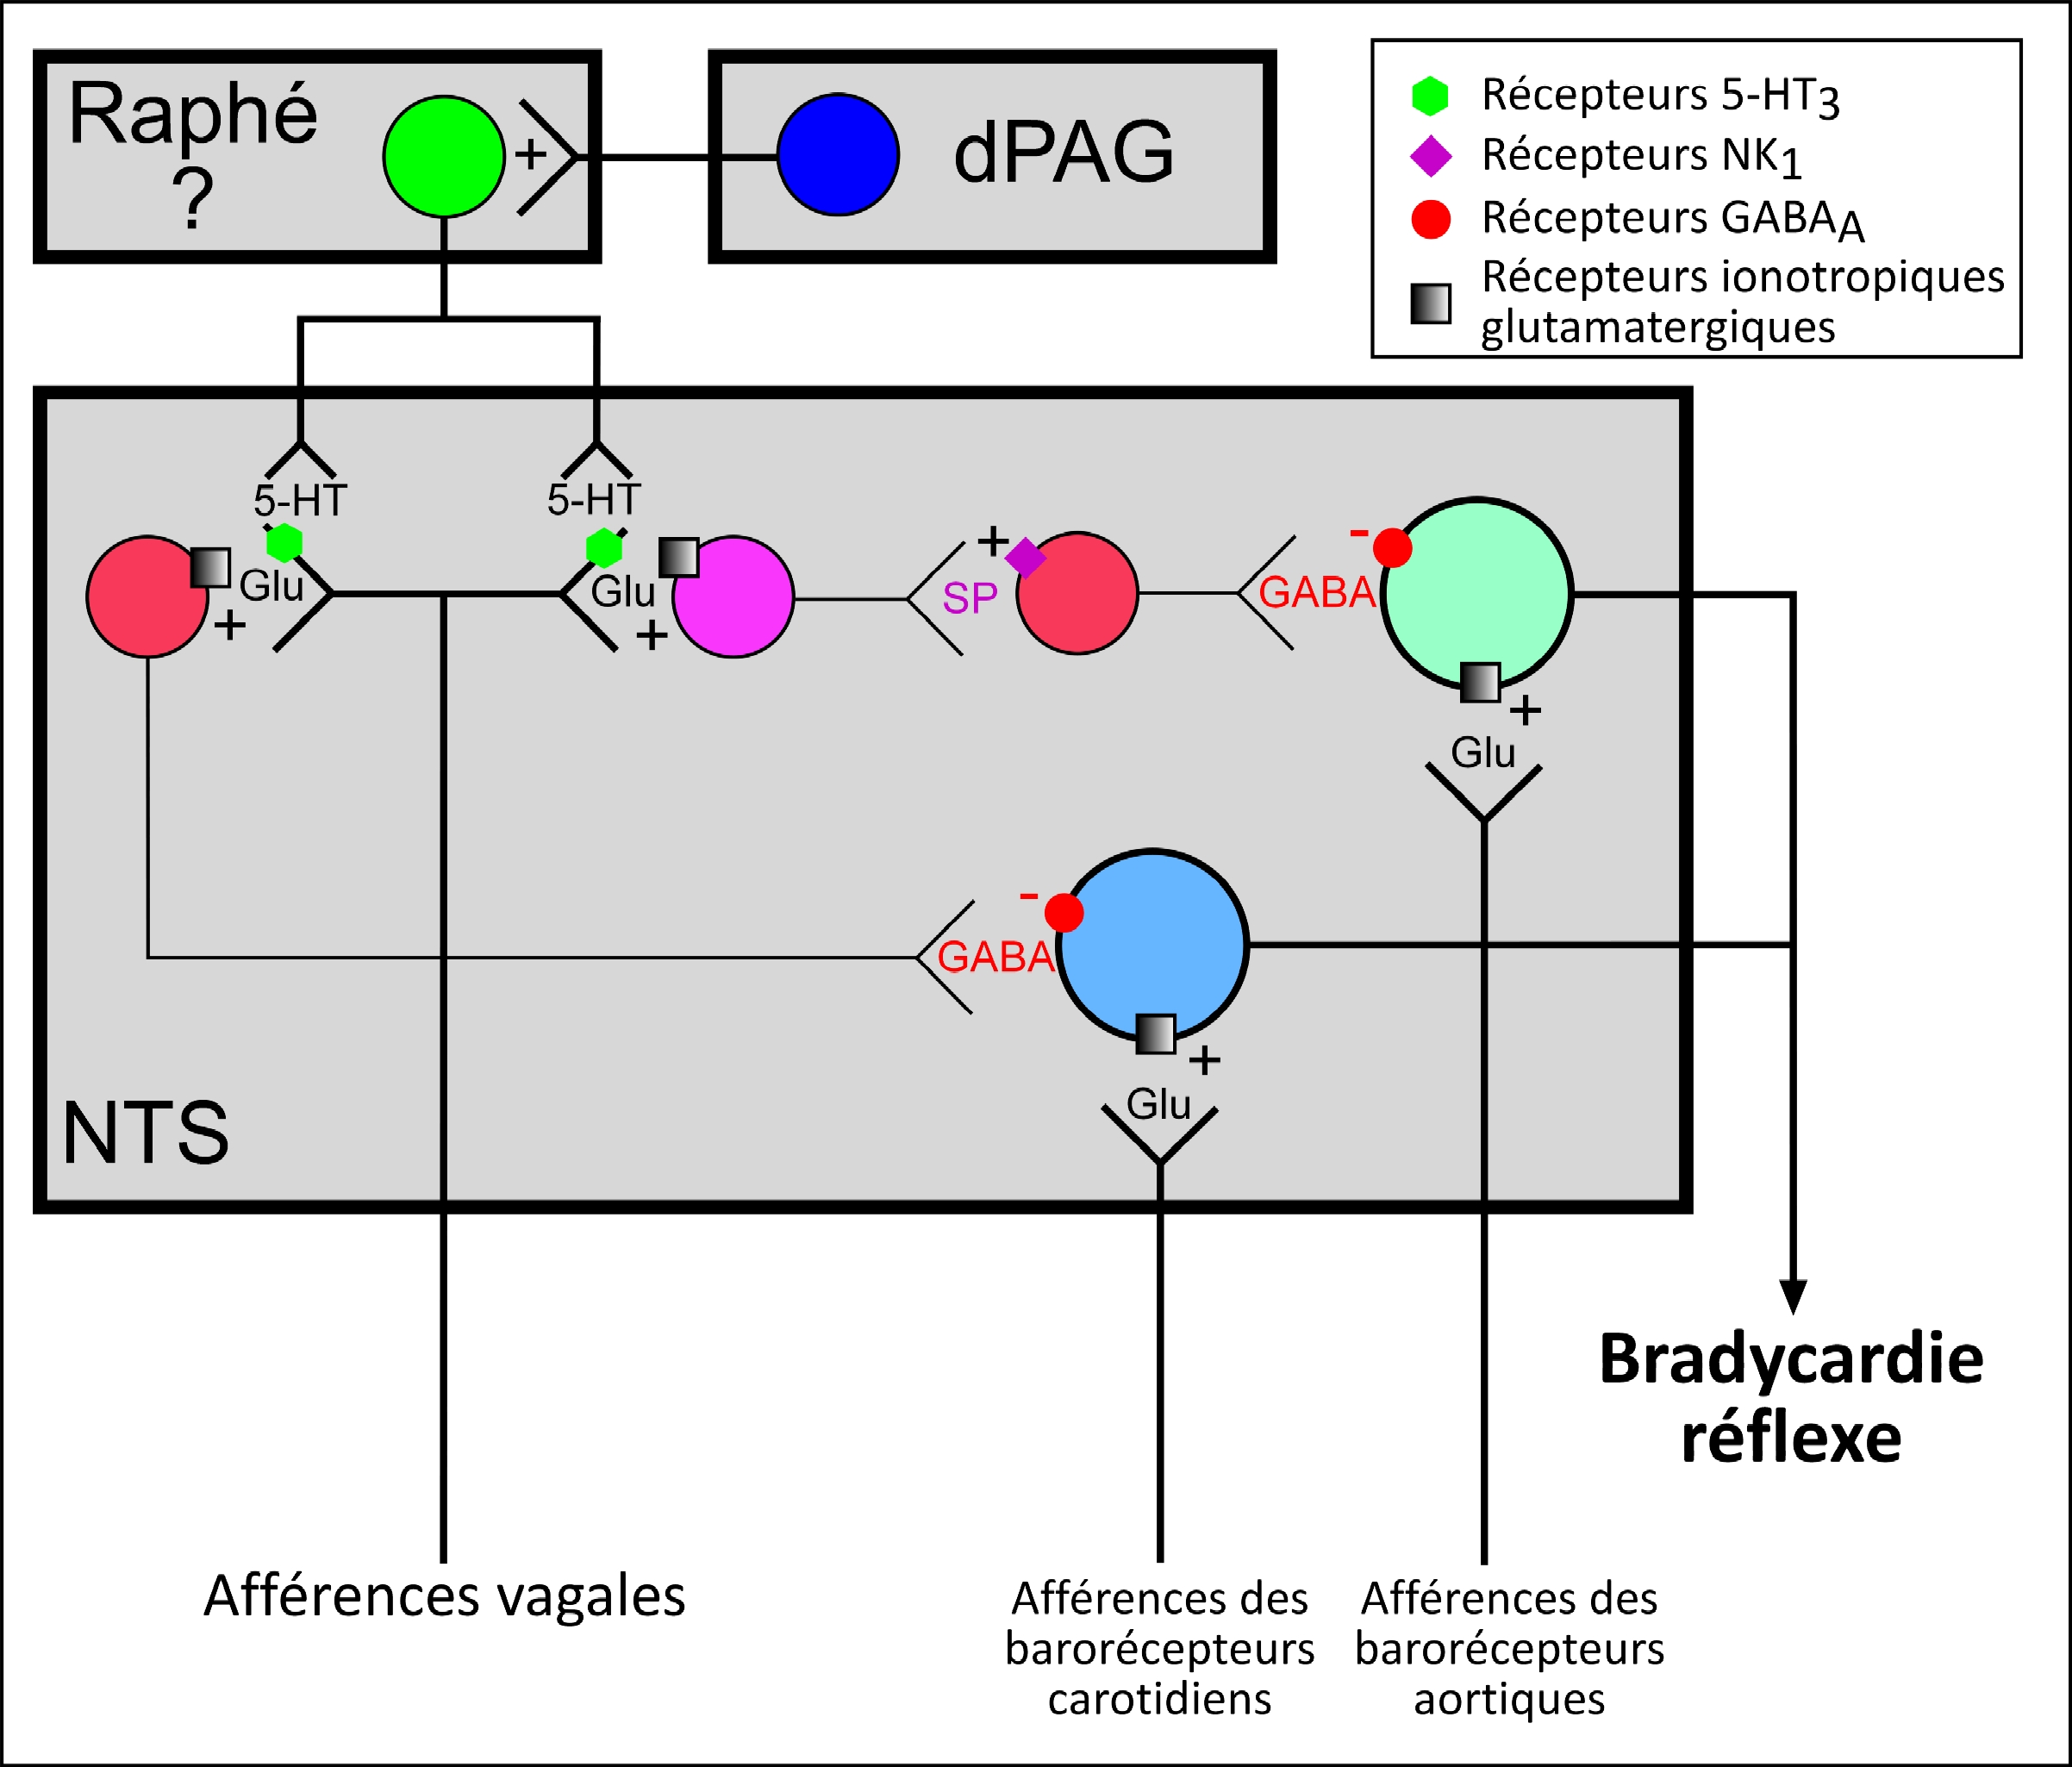
\includegraphics[width=16cm]{Figure10.jpg} 
\end{center}

\caption{\textbf{Rôle fonctionnel des récepteurs 5-HT$_{3}$, NK$_{1}$ et GABA$_{A}$ du NTS}}

{\protect\parbox[t]{18cm}{
\begin{small}
Schéma représentant le circuit neurochimique hypothétique sous tendant l’inhibition de la bradycardie du baroréflexe pendant la réaction de défense.\\ 
5-HT : sérotonine ; dPAG : Colonne dorsale de la substance grise périaqueducale ; Glu : Glutamate ; SP : substance P (Figure modifiée à partir de Comet et al. 2005)
\end{small}}}

\label{Figure 10}

\end{figure}

\section{Nociception et réaction de défense : effets cardiovasculaires}

\label{Nociception,réaction de défense,effets cardiovasculaires}

Les paramètres cardiovasculaires sont modulés en fonction des conditions environnementales dans le but de produire une réponse adaptée de l’organisme. De nombreuses situations physiologiques peuvent illustrer ces mécanismes adaptatifs comme, par exemple, la réaction de défense déclenchée en réponse à un stimulus nociceptif, stressant ou dangereux. 

En réponse à la perception d’un danger, tous les mammifères présentent une réaction d’alerte qui peut conduite à un comportement agressif ou défensif. Ce comportement d’attaque ou de fuite s'accompagne aussi de modifications végétatives qui se traduisent, entre autres, par une mydriase, une piloérection et une posture agressive/défensive de l’animal. On observe aussi des modifications cardiovasculaires : augmentation du débit cardiaque, de la fréquence cardiaque, de la pression artérielle, avec une redistribution du flux sanguin (Depaulis \& Bandler 1991), permettant de répondre à la demande énergétique accrue de la musculature striée de l’animal. Une vasodilatation intervient au niveau des muscles volontaires, alors que, au niveau cutané et viscéral, le flux est diminué par vasoconstriction (Nosaka 1996; Nalivaiko \& Blessing 2001). Ces effets cardiovasculaires sont le résultat d’une sympathoexcitation (Verberne et al. 1989; Nosaka 1996). Ils peuvent être déclenchés même sous anesthésie légère par une stimulation nociceptive somatique aussi bien chez l’animal (Blessing \& Nalivaiko 2000; Boscan et al. 2005) que chez l’être humain (Mashimo et al. 1997; Shimoda et al. 1998; Jeanne et al. 2009)
\footnote{Il est intéressant de noter que la relation qui existe entre douleur et pression artérielle est à double-sens : comme décrit ci-dessus une stimulation douloureuse entraîne une élévation de pression artérielle, mais réciproquement, chez l’individu sain, une pression artérielle élevée est associée à un seuil de douleur élevé. Les deux phénomènes impliquent d’ailleurs des structures cérébrales très proches et font probablement toutes deux appel, en partie, aux opioïdes endogènes. Cette relation douleur $\Longleftrightarrow$ pression artérielle est altérée chez des patients souffrant de douleurs chroniques (Bruehl \& Chung 2004).}.

Lors d’une réaction de défense ou lors d’une stimulation nociceptive somatique, la tachycardie et la vasoconstriction viscérale, entraînent une élévation de la pression artérielle suffisante pour déclencher le baroréflexe. On devrait donc observer une diminution compensatoire de la pression artérielle. En réalité, dans ces situations la bradycardie du baroréflexe est inhibée permettant la redistribution des flux sanguins, nécessaire à la bonne exécution de la conduite. (Nosaka \& Murata 1989; Nosaka 1996; Boscan et al. 2002a; Boscan et al. 2002b; Pickering et al. 2003).

\subsection{Structures et neurotransmetteurs impliqués}

La substance grise périaqueducale (PAG) est la principale structure impliquée dans la réaction de défense. Cette structure est formée par des colonnes de neurones orientées selon l’axe caudorostral (Carrive 1993; Bandler \& Shipley 1994). C’est la région dorsolatérale de la PAG (dlPAG) qui joue un rôle clé dans la réaction de défense (Hockman \& Talesnik 1971; Carrive et al. 1987; Nosaka et al. 1993; Nosaka 1996; Bandler et al. 2000). 

D'autres structures participent aussi à la réaction de défense, notamment l’hypothalamus et, plus précisément, un groupe de noyaux hypothalamiques constituant l’« aire de défense hypothalamique » (Nosaka et al. 1989; Smith \& Barron 1989; Nosaka 1996). Celle-ci inclut notamment les noyaux dorsomédian (DMH) et ventromédian (VMH) de l’hypothalamus (Gebber \& Snyder 1970; Coote et al. 1979; Hilton \& Redfern 1986; Yardley \& Hilton 1986; Lammers et al. 1988; DiMicco et al. 1996; DiMicco et al. 2002). Enfin, le noyau parabrachial et l’amygdale semblent également impliqués dans cette conduite (Nosaka 1996).

La stimulation, électrique ou pharmacologique, du DMH, du VMH ou de la dlPAG entraîne, chez l’animal éveillé ou anesthésié, certaines des manifestations périphériques (piloérection, mouvements des vibrisses, exorbitation ophtalmique\ldots) ainsi que toutes les modifications cardiovasculaires caractéristiques de la réaction de défense : hypertension, tachycardie (Carrive et al. 1987; Hamalainen \& Lovick 1997), dont l’inhibition de la bradycardie du baroréflexe (Gebber \& Snyder 1970; Hockman \& Talesnik 1971; Coote et al. 1979; Nosaka et al. 1993). L’augmentation de la pression artérielle et la tachycardie observées pendant la réaction de défense sont d’origine sympathique, et mettent en jeu des neurones sympathoexcitateurs de la RVL (Carrive et al. 1988; Lovick 1992; 1993).

Dans le cas de la nociception, le noyau parabrachial semble jouer un rôle important dans la tachycardie induite par une stimulation somatique (Boscan et al. 2005), soit via une projection directe vers la RVL, soit indirectement via le DMH, le VMH ou la dlPAG.

Plus récemment, il est apparu que, associé à la nociception et/ou à la réaction de défense, la RVM joue un rôle important dans certaines des réponses cardiovasculaires (Blessing \& Nalivaiko 2000; Nalivaiko \& Blessing 2001; Nason \& Mason 2004; Nalivaiko et al. 2005). De fait, cette région serait au moins responsable de la régulation des flux sanguins cutanés, et notamment de leur réduction lors d’une stimulation nociceptive ou lors d’une stimulation du DMH (Blessing \& Nalivaiko 2000; Nalivaiko \& Blessing 2001; 2002). Ainsi, en plus de son action spinale sur le maintien du tonus sympathique (Mc Call 1984), la RVM, et particulièrement les neurones sérotoninergiques de cette région, contrôlerait la vascularisation cutanée implique (Blessing 2004; Nalivaiko et al. 2005; Ootsuka \& Blessing 2005).

Le fait que la composante parasympathique du baroréflexe est inhibée lors d’une réaction de défense, associé à l’existence d’un circuit inhibiteur de cette composante impliquant les récepteurs 5-HT$_{3}$, a amené à proposer l’hypothèse que l’inhibition pendant une réaction de défense pouvait être sous-tendue par la sérotonine et l’activation de récepteurs 5-HT$_{3}$ du NTS. Cette hypothèse a été confirmée par plusieurs données :

\begin{itemize}
\item L’inhibition de la composante parasympathique du baroréflexe lors d’une stimulation de la dlPAG n’est pas observée lorsque les animaux ont subi un traitement préalable à la pCPA pour bloquer la synthèse de sérotonine (Comet et al. 2004). 
\item Cette inhibition est prévenue par la microinjection préalable d’un antagoniste des récepteurs 5-HT$_{3}$ dans le NTS (Sevoz-Couche et al. 2003; Comet et al. 2004).
\item Cette inhibition est absente chez des souris KO pour le récepteur 5-HT$_{3}$ (Netzer et al. En préparation)
\end{itemize}

Au vu des interactions fonctionnelles décrites ci-dessus entre les récepteurs 5-HT$_{3}$, NK$_{1}$ et GABA du NTS, et sachant que l’inhibition de la composante parasympathique du baroréflexe pendant une réaction de défense implique un maillon GABAergique (Nosaka et al. 1989; Spyer 1994; Sevoz-Couche et al. 2003; Comet et al. 2004), le modèle suivant a été proposé pour expliquer cette inhibition (voir Figure \ref{Figure 10} - page \pageref{Figure 10}) :

Lors d’une réaction de défense, la sérotonine libérée dans le NTS active les récepteurs 5-HT$_{3}$ présynaptiques sur les afférences vagales. L’excitation qui en résulte déclenche la libération de glutamate.

Au sein du NTS, cet acide-aminé excitateur active deux groupes distincts de neurones : des interneurones SPergiques et des interneurones GABAergiques.

\begin{itemize}
\item La Substance P, libérée par les premiers, active des récepteurs NK$_{1}$ localisés sur des neurones GABAergiques, ceux-ci inhibant secondairement les cellules, normalement excitées par les afférences des barorécepteurs aortiques et responsables de la production des réponses cardiaques réflexes.
\item Le GABA libéré active des récepteurs GABA$_{A}$ localisés sur des cellules, également impliquées dans la production des réponses cardiaques réflexes mais recevant des afférences provenant des barorécepteurs carotidiens.
\end{itemize}

Dans les deux cas, l’activation de récepteurs GABA$_{A}$ est à l’origine de l’inhibition de la bradycardie réflexe.

Il est important de préciser que l’ensemble de ces résultats concerne la composante parasympathique du baroréflexe. La composante sympathique (hypotension et bradycardie modérée) ne serait pas modifiée par la réaction de défense (Nosaka et al. 1993; Sevoz-Couche et al. 2003).

Enfin, il convient de rappeler que l’implication de la substance P et du GABA, dans l’inhibition de la composante parasympathique du baroréflexe par un stimulus nociceptif, a également été montrée (Boscan \& Paton 2001; Boscan et al. 2002a; Pickering et al. 2003). Mais le modèle décrit ci-dessus ne peut pas être d’ores et déjà étendu au cas de la nociception, puisque les rôles éventuels de la sérotonine et des récepteurs 5-HT$_{3}$ n’ont pas encore été étudiés dans les situations expérimentales ad hoc.

\cleardoublepage

\fancyhf{} % delete current header and footer
\fancyfoot[C]{\bfseries -\thepage-}
\fancyhead[RO]{\bfseries\rightmark}
\fancyhead[LE]{\bfseries R\'ESULTATS - 5-HT, baroréflexe et réaction de défense}
\renewcommand{\headrulewidth}{1pt}
\renewcommand{\footrulewidth}{1pt}
\addtolength{\headheight}{1pt} % space for the rule

\part{RÉSULTATS}

\cleardoublepage

\chapter{Quelle est l’origine de la sérotonine libérée dans le NTS pendant la réaction de défense ?}

\section{PRÉAMBULE}

\subsection{Introduction}

En réponse à une agression physique ou à un stress psychique, les mammifères présentent un comportement d’alerte qui peut conduire à un comportement agressif ou défensif. Lors d’une telle de réaction de défense, la pression artérielle et la fréquence cardiaque augmentent fortement pour accroître le flux sanguin au niveau des muscles squelettiques et permettre une réponse adaptée. En accord avec ce besoin physiologique (Nosaka 1996), plusieurs études ont montré que la composante parasympathique du baroréflexe (i.e. bradycardie) est inhibée dans des modèles de réactions de défense (e.g. stimulation de la colonne dorsolatérale de la substance grise périaqueducale - dlPAG) (Inui \& Nosaka 1993; DiMicco et al. 2002; Sevoz-Couche et al. 2003). 

Des études récentes montrent que la libération de sérotonine est nécessaire à l’inhibition de la bradycardie du baroréflexe par une stimulation de la dlPAG (Comet et al. 2004). En effet, cette inhibition est reproduite par des microinjections d’agonistes des récepteurs 5-HT$_{3}$ (Merahi et al. 1992b) dans le noyau du tractus solitaire (NTS) où projettent les barorécepteurs (Reis et al. 1981). À l’inverse, les effets d’une stimulation de la dlPAG sur cette bradycardie réflexe, sont prévenus par des microinjections intra-NTS d’antagonistes des récepteurs 5-HT$_{3}$ (Sevoz-Couche et al. 2003; Comet et al. 2004). Il a donc été proposé que la libération de sérotonine dans le NTS activent les récepteurs 5-HT$_{3}$, situés en position présynaptique sur les afférences vagales glutamatergiques (Merahi et al. 1992b). La libération de glutamate qui en découle permet l’inhibition, via un interneurone GABA, les neurones à l’origine de la réponse cardiovagale du baroréflexe (Sevoz-Couche et al. 2003; Comet et al. 2004).

\subsection{Objectif de l’étude}

\textbf{Les neurones sérotoninergiques activés pendant une stimulation de la dlPAG et à l’origine de la libération de sérotonine dans le NTS n’étaient pas encore identifiés à cette époque. Cette première étude a donc eu pour but de mettre en évidence le groupe de neurones sérotoninergiques à l’origine de l’inhibition de la composante parasympathique du baroréflexe.}

Dans la première partie de ce travail, nous avons identifié les neurones sérotoninergiques activés par la stimulation électrique de la dlPAG, en utilisant la technique du c-fos couplée à un immunomarquage de la sérotonine. 

Dans un deuxième temps, nous avons montré l’implication fonctionnelle du groupe de neurones sérotoninergiques identifié par le c-fos. 

\begin{enumerate}
\item Nous avons examiné l’effet de l’inactivation pharmacologique de ce groupe par microinjection locale de muscimol (un agoniste des récepteurs GABA $_{A}$) ou de 8-OH-DPAT (un agoniste des récepteurs 5-HT$_{1A}$ ) sur l’inhibition de la composante parasympathique du baroréflexe induite par une activation électrique ou pharmacologique de la dlPAG. 
\item Nous avons ensuite examiné l’effet de l’activation pharmacologique de ce groupe par microinjection locale d’acide D, L homocystéique (DLH) sur la bradycardie du baroréflexe. 
\item La spécificité « sérotoninergique » des ces effets a été contrôlée en les réexaminant après une microinjection de granisétron, un antagoniste des récepteurs 5-HT$_{3}$, dans le NTS.\end{enumerate}

\subsection{Résultats}

\subsubsection{Étude c-fos des neurones sérotoninergiques activés par une stimulation de la dlPAG}

La stimulation électrique de la dlPAG (50 Hz ; durée des pulses : 1 ms ; 150 µA ; durée totale de stimulation 20 min), sur un groupe de 6 rats « expérimentaux » anesthésiés à l’uréthane, entrainait bien une élévation de la pression artérielle et de la fréquence cardiaque caractéristique de la réaction de défense. Chez 5 animaux « contrôles », l’électrode de stimulation a été mise en place, mais aucune stimulation n’a été appliquée.

La comparaison dans le groupe expérimental et dans le groupe contrôle du nombre des neurones marqués dans les noyaux du raphé dorsal (RDr), obscurus (ROb), pallidus (RPa) et magnus (RMg), ainsi dans le noyau latéral paragigantocellulaire (LPGi), a montré que \textbf{l’activation de la dlPAG n'induisait une augmentation du marquage c-fos dans les neurones sérotoninergiques qu'au niveau du groupe B3 (RMg et LPGi), essentiellement dans le milieu de son étendue rostro-caudale (Article 1 - Fig. 1 B1-B2)}. L’augmentation du nombre de neurones doublement marqués était de 94 \% dans le LPGi et 101 \% dans le RMg (Article 1 - Fig. 2 A-B). Le pourcentage de neurones sérotoninergiques exprimant la protéine c-fos (par rapport au nombre total de neurones sérotoninergiques) a augmenté de 52 $\pm$ 3 \% (groupe contrôle) à 79 $\pm$ 3 \% (groupe expérimental) dans le LPGi, et de 20 $\pm$ 2 \% (groupe contrôle) à 43 $\pm$ 4 \% (groupe expérimental) dans le RMg. 

\textbf{Aucune augmentation significative du marquage c-Fos n’a été observée dans les autres groupes sérotoninergiques (Article 1 - Fig. 4 A-C)}. Dans les groupes contrôle et expérimental, le pourcentage de neurones sérotoninergiques exprimant la protéine c-fos (par rapport au nombre total de neurones sérotoninergiques), étaient, respectivement, de 9 $\pm$ 3 \% et 12 $\pm$ 2 \% dans le RPa, de 9 $\pm$ 4 \% et 11 $\pm$ 3 \% dans le ROb (Article 1 - Fig. 3 C-D) et de 0,8 $\pm$ 0,6 \% et 1,3 $\pm$ 0,3 \% dans le RDr (Article 1 - Fig. 3 E-F).

Ces observations suggèrent que le groupe B3 est la principale source de sérotonine libérée dans le NTS pendant la réaction de défense induite par la stimulation de la dlPAG.
Dans la région rostroventromédiane du bulbe (RVM), une augmentation de 167 \% du nombre de neurones non-sérotoninergiques exprimant la protéine c-fos a aussi été observée (Article 1 - Fig. 1 A3). 

\subsubsection{Effet de l’inhibition et de l’activation pharmacologique de la RVM }

L’activation électrique (50 Hz ; pulses : 1 ms ; 150 µA ; pendant 5 s ; n = 5) (Article 1 – Fig. 6 A) ou pharmacologique (DLH ; 0,3 M ; 100 nL ; n = 15) de la dlPAG entraînait, chez des rats anesthésiés à l’uréthane : une forte augmentation de la pression artérielle moyenne (45 $\pm$ 5 et 45 $\pm$ 4 mmHg respectivement), de la fréquence cardiaque (70 $\pm$ 10 et 74 $\pm$ 9 bpm respectivement) ainsi qu’une inhibition de, respectivement, 70 \% de la bradycardie réflexe induite par stimulation du nerf aortique (Article 1 - Fig. 5 A-B).

\textbf{Après l’inactivation pharmacologique du groupe B3 par microinjection de muscimol (5 mM, 100 nL) dans la RVM (Article 1 – Fig. 6 B), l’activation électrique ou par le DLH de la dlPAG n’inhibait plus la bradycardie du baroréflexe que de, respectivement, 17 et 12 \% (Article 1 - Fig. 5 A-B).} De même, après l’inactivation pharmacologique de la RVM par microinjection de 8-OH-DPAT (30 mM ; 100 nL ; n = 14), la diminution de la bradycardie du baroréflexe induite par l’activation de la dlPAG n’était plus que de 14 \% (Résultats supplémentaires article 1). 

La stimulation directe des neurones du groupe B3 par activation pharmacologique de la RVM (DLH ; 0,3 M ; 100 nL ; n = 16) (Article 1 – Fig. 7) augmentait fortement la pression artérielle moyenne et de la fréquence cardiaque (22 $\pm$ 2 mmHg et 40 $\pm$ 5 bpm respectivement) et \textbf{inhibait la bradycardie du baroréflexe de 55 \% (Article 1 – Fig. 8)}. 

\subsubsection{Effet du blocage des récepteurs 5-HT$_{3}$ du NTS}

Cette dernière série d'expérience avait pour but de nous assurer que l’activation des cellules sérotoninergiques du groupe B3 était le facteur critique dans l'inhibition de la bradycardie du baroréflexe observée pendant l’activation pharmacologique de la RVM. Ainsi, nous avons examiné l'effet de microinjections intra-NTS de granisétron, un antagoniste spécifique des récepteurs 5-HT$_{3}$ .

\textbf{Avec une telle microinjection (2,5 mM, 100 nL, n = 7) (Article 1 – Fig. 6 C), l’inhibition de la bradycardie du baroréflexe induite par l’activation pharmacologique de la RVM était complètement réversée (Article 1 – Fig. 8).} 

\subsection{Discussion et conclusion}

Le NTS reçoit des afférences sérotoninergiques des noyaux du RDr, du ROb, du RPa et du groupe B3 (LPGi et RMg) (Thor \& Helke 1987; Schaffar et al. 1988). Nos résultats montrent que, parmi ces différents noyaux, c’est seulement au milieu de l’étendue rostro-caudale du groupe B3 que l’on observe une augmentation du nombre de neurones sérotoninergiques exprimant la protéine c-fos après une stimulation de la dlPAG. Nous avons donc supposé que ces neurones sérotoninergiques activés étaient impliqués dans l’inhibition de la composante parasympathique du baroréflexe lors d’une stimulation de la dlPAG, car celle-ci nécessite une libération de sérotonine au niveau du NTS (voir introduction). Toutefois, la protéine c-fos n’est qu’un témoin indirect de l’excitation des neurones sérotoninergiques, qui ne permet pas de connaître exactement le phénomène à l’origine de cette activation.

L’approche pharmacologique utilisée montre l’importance fonctionnelle de la région du groupe B3 dans l’inhibition de la bradycardie du baroréflexe par une stimulation de la dlPAG, puisque l’inactivation des neurones de cette région par le muscimol prévient effectivement cette inhibition. Les effets similaires obtenus avec une microinjection de 8-OH-DPAT, inhibant les neurones sérotoninergiques de manière plus spécifique (Fornal et al. 1985; McCall \& Clement 1989; McCall et al. 1989; Clement \& McCall 1991), renforce l’hypothèse d’un rôle préférentiel des neurones sérotoninergiques. Le fait que l’activation pharmacologique du groupe B3, par une microinjection locale de DLH, suffit à induire l’inhibition la bradycardie du baroréflexe renforce notre conclusion.

Toutefois, les récepteurs GABA $_{A}$ et les récepteurs glutamatergiques ionotropiques sont des quasi-ubiquitaires. Des injections de muscimol et de DLH auront donc tendance à, respectivement, hyperpolariser et dépolariser toutes les cellules de la RVM et des régions avoisinantes où l’injection a diffusé et pas seulement les neurones sérotoninergiques du groupe B3. Pour montrer le rôle critique des neurones sérotoninergiques du groupe B3 dans cette inhibition, nous avons testé les effets d’une microinjection de granisétron, un antagoniste spécifique des récepteurs 5-HT$_{3}$, dans le NTS. Une telle microinjection permet de lever quasi-complètement l’inhibition du baroréflexe cardiovagal induite par une activation de la RVM. 

L’ensemble de ces données nous a amené à proposer un modèle théorique du circuit « dlPAG-B3-NTS » sous-tendant l’inhibition la composante parasympathique du baroréflexe lors d’une réaction de défense (Article 1 - Fig. 9). L’activation de la dlPAG, qui projette fortement sur la RVM (Cameron et al. 1995; Hermann et al. 1997) et sur les neurones sérotoninergiques du groupe B3 (Braz et al. 2009), induit l’activation de ces derniers. Ceux-ci, projetant sur NTS (Thor \& Helke 1987; Schaffar et al. 1988), libère de la sérotonine dans ce noyau, et permettent l’inhibition des neurones recevant les afférences provenant des barorécepteurs, via l’activation glutamatergique d’interneurones GABAergiques.

\cleardoublepage

\section{ARTICLE 1}

\vfill

\begin{center}

\begin{LARGE}
\textbf{CRITICAL ROLE OF B3 SEROTONERGIC CELLS IN BAROREFLEX INHIBITION DURING THE DEFENSE REACTION TRIGGERED BY DORSAL PERIAQUEDUCTAL GRAY STIMULATION}
\end{LARGE}

\bigskip

\begin{large} 
\textbf{BERNARD Jean-François, NETZER Florence, GAU Rémi, HAMON Michel, LAGUZZI Raùl, SÉVOZ-COUCHE Caroline} \end{large}

\bigskip

Journal of comparative anatomy, 2008 Jan 1 ; 506 (1) : 108-21

DOI : 10.1002/cne.21532

\vfill

\end{center}

\cleardoublepage

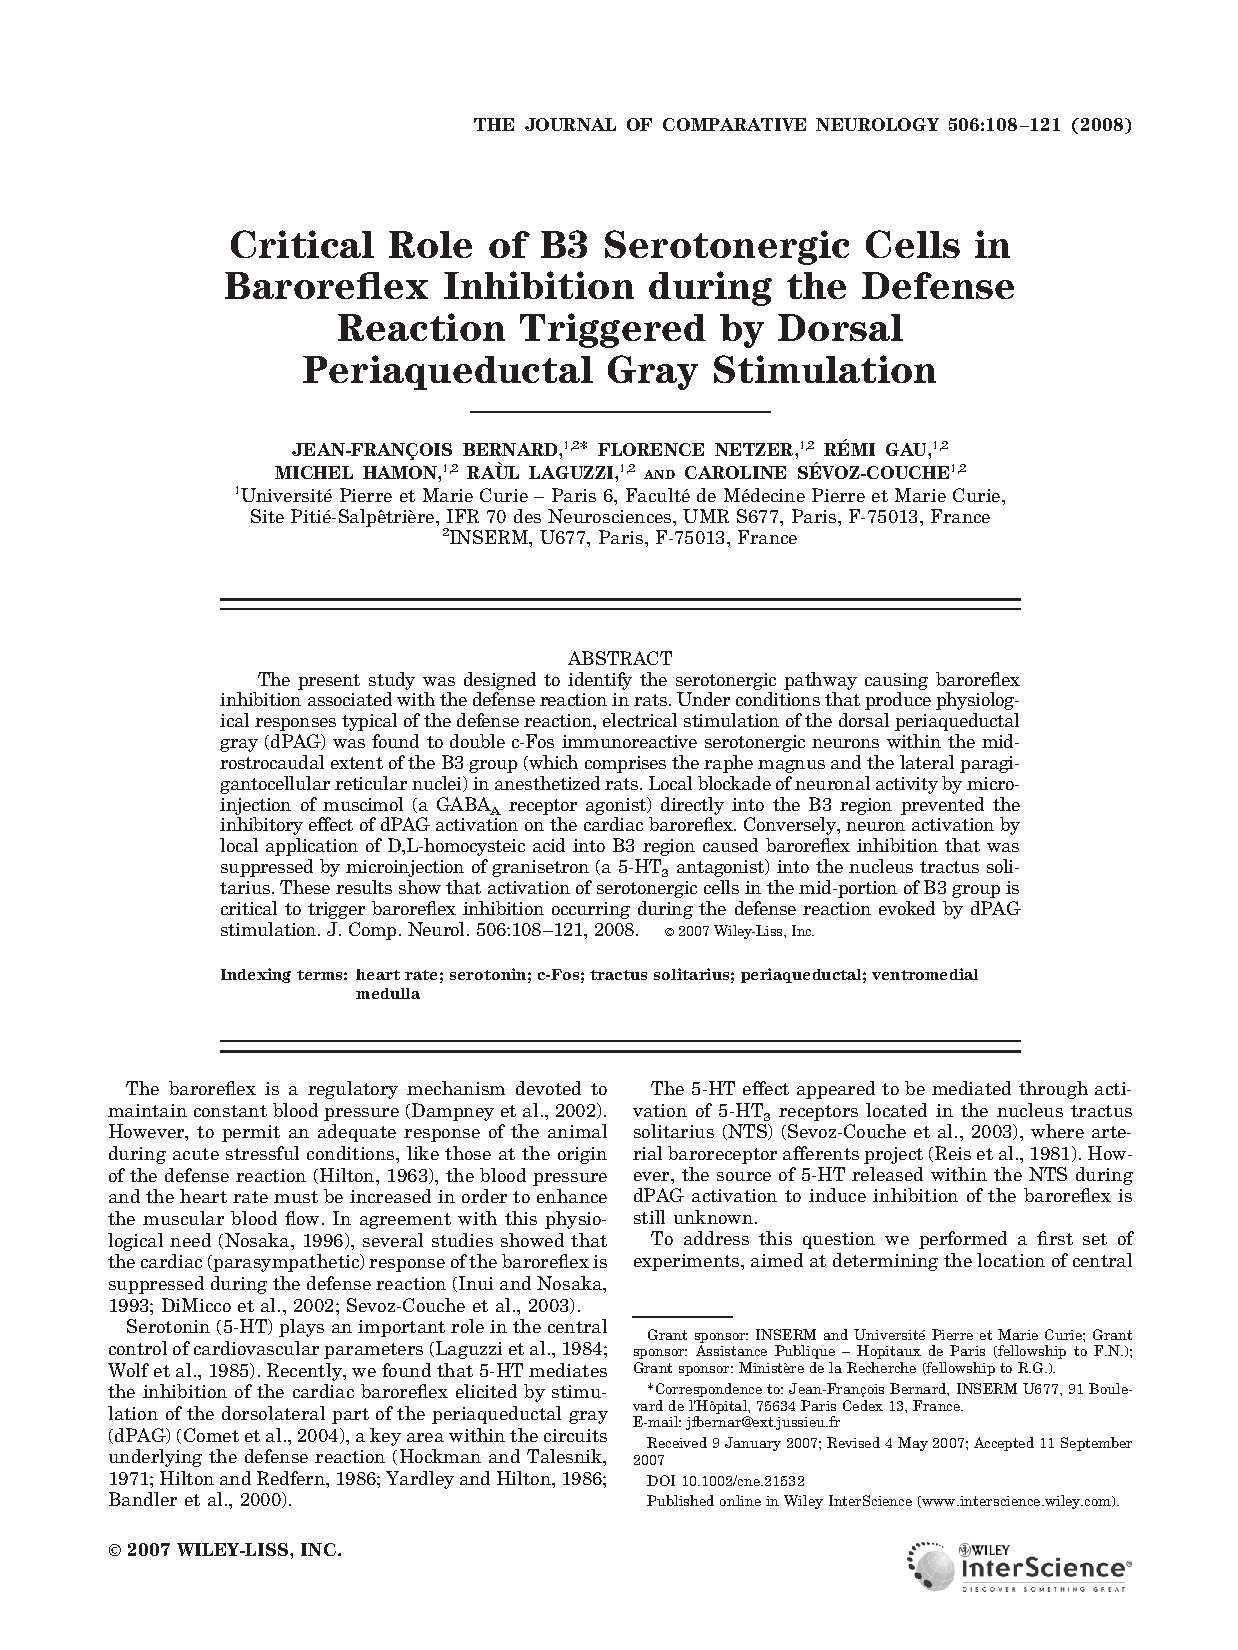
\includepdf[pages={1-14}]{2008Bernard.pdf}

\cleardoublepage

\section{RÉSULTATS SUPPLÉMENTAIRES}

\subsection{Introduction}

Le récepteur 5-HT$_{1A}$ est un récepteur métabotropique inhibiteur. Son ARNm est exprimé par 70 \% des neurones sérotoninergiques de la RVM et 60 \% des neurones qui expriment cet ARNm sont sérotoninergiques (Zhang et al. 2000a). Ainsi, les récepteurs 5-HT$_{1A}$ sont aussi présents sur un nombre plus faible, mais non négligeable, de neurones non-sérotoninergiques. Toutefois, les expériences d’électrophysiologie \textit{in-vivo} montre que l’activation de ce récepteur par un agoniste comme le 8-OH-DPAT inhibe préférentiellement, et de manière relativement spécifique, les neurones présumés sérotoninergiques de cette région (Fornal et al. 1985; McCall \& Clement 1989; McCall et al. 1989; Clement \& McCall 1991).

Dans la deuxième série d’expériences de l’article 1, nous avons utilisé le muscimol pour inactiver l’ensemble de la RVM, et montrer l’implication fonctionnelle de cette région dans l’inhibition de la composante parasympathique du baroréflexe lors d’une stimulation de la dlPAG. En effet, le muscimol est une substance qui agit sur les récepteurs GABA $_{A}$, quasi ubiquitaire, et inhibe donc presque tous les neurones. 

Nous avons donc aussi réalisé des microinjections de 8-OH-DPAT, afin d’inhiber de manière plus spécifique les neurones sérotoninergiques de cette région, et ainsi préciser leur implication dans l’inhibition de la bradycardie du baroréflexe lors d’une stimulation de la dlPAG.

Ces expériences ont suivi le même protocole que celui utilisé pour les microinjections de muscimol (voir matériels et méthodes de l’article 1 : expérience 2).

\subsection{Résultats}

\paragraph{Effets de microinjections de 8-OH-DPAT dans la RVM sur les réponses cardiovasculaires induites par l’activation pharmacologique de la dlPAG}

Alors qu’une activation pharmacologique de la dlPAG réduit de 68 \% la bradycardie induite par une stimulation du nerf aortique, cette inhibition n’était plus que de 14 \%, lorsqu’une microinjection de 8-OH-DPAT (30 mM ; 100 nL ; n = 14) dans la RVM a été réalisée au préalable (réponse cardiovagale aortique [ACR] « contrôle » : -0,28 $\pm$ 0,04 ; ACR « expérimentale » : -0,25 $\pm$ 0,04 ; 3-way ANOVA ; p<0,005). 

Ces microinjections n’avaient pas d’effet, par elles-mêmes, sur la fréquence cardiaque, qui était diminuée de seulement 9 $\pm$ 5 bpm pour une valeur de base 395 $\pm$ 15 bpm, ou sur la pression artérielle, qui diminuait de seulement 5 $\pm$ 3 mmHg pour une valeur au repos de 102 $\pm$ 8 mmHg. 

De même, le 8-OH-DPAT ne modifiait pas les effets d’une activation pharmacologique de la dlPAG sur la pression artérielle et sur la fréquence cardiaque. L’injection de DLH dans la dlPAG induisait une réponse pressive de +43 $\pm$ 4 mmHg (n = 15), qui était inchangée (+49 $\pm$ 5 mmHg) après injection de 8-OH-DPAT dans la RVM. De même, la tachycardie observée après activation de la dlPAG (74 $\pm$ 9 bpm) n’était pas modifiée (70 $\pm$ 4 bpm) par cette injection. 

\subsection{Discussion et conclusion}

Les effets du 8-OH-DPAT étant comparables à ceux du muscimol, ces résultats montrent que seulement sous-groupe de neurones de la RVM est nécessaire à l’inhibition de la bradycardie du baroréflexe pendant une stimulation de la dlPAG. Les premiers travaux réalisés au niveau du raphé dorsal ont montré que presque tous les neurones de ce noyau exprimant le récepteur 5-HT$_{1A}$ sont sérotoninergiques (Sotelo et al. 1990). Dans la RVM toutefois, ce récepteur semble être exprimé par certains neurones non-sérotoninergiques et seulement par un-sous groupe de neurones sérotoninergiques (Helke et al. 1997; Zhang et al. 2000a). Ces résultats, pris indépendamment de ceux des expériences de c-fos et des microinjections de granisétron dans le noyau du tractus solitaire, ne permettent pas d’exclure de façon stricte un rôle potentiel des neurones non-sérotoninergiques de la RVM dans l’inhibition de la bradycardie du baroréflexe. 

Toutefois, plusieurs études d’électrophysiologie \textit{in-vivo} montrent que les agonistes des récepteurs 5-HT$_{1A}$, dont le 8-OH-DPAT, inhibent la très grande majorité des neurones sérotoninergiques de cette région. Dans ces travaux, les neurones sérotoninergiques sont identifiés indirectement par leur décharge lente et régulière et par au moins un des critères suivants : 1) des potentiels d’action de longue durée, 2) une vitesse de conduction très faible, 3) une activité dépendante de l’état de veille. Ces neurones voient leur activité spontanée diminuer, ou sont complètement inhibés par les agonistes des récepteurs 5-HT$_{1A}$ administrés par voie systémique ou par iontophorèse (Wessendorf \& Anderson 1983; Auerbach et al. 1985; Chiang \& Pan 1985; Fornal et al. 1985; Wei \& Chiang 1986; McCall \& Clement 1989; McCall et al. 1989; Clement \& McCall 1991). Les mêmes études montrent que les neurones ne présentant pas ces caractéristiques électrophysiologiques, et donc très probablement non-sérotoninergiques, sont, pour la plupart, insensibles à ces agonistes, même avec des doses 10 à 100 fois plus fortes que la dose affectant les neurones sérotoninergiques.

Ce constat que le 8-OH-DPAT semble préférentiellement inhiber les neurones sérotoninergiques, associé aux faits que : 1) la technique du c-fos montre une activation préférentielle de ces neurones après une stimulation de la dlPAG, et que 2) la microinjection d’un antagoniste des récepteurs 5-HT$_{3}$ dans le NTS permet de lever l’inhibition du baroréflexe cardiaque par une activation de la RVM, renforce l’idée que ce sont essentiellement les neurones du groupe B3 qui constitue le maillon sérotoninergique de cette inhibition.

\cleardoublepage

\fancyhf{} % delete current header and footer
\fancyfoot[C]{\bfseries -\thepage-}
\fancyhead[RO]{\bfseries\rightmark}
\fancyhead[LE]{\bfseries R\'ESULTATS - 5-HT, baroréflexe et nociception}
\renewcommand{\headrulewidth}{1pt}
\renewcommand{\footrulewidth}{1pt}
\addtolength{\headheight}{1pt} % space for the rule

\chapter{Quelle est le rôle de la sérotonine dans l’inhibition de la bradycardie du baroréflexe par une stimulation nociceptive ?}

\section{PRÉAMBULE}

\subsection{Introduction}

Les stimulations nociceptives somatiques entraînent des augmentations généralement intenses de la pression artérielle et de la fréquence cardiaque, même sous anesthésie légère (Sun \& Spyer 1991; Mashimo et al. 1997; Boscan \& Paton 2001; Nason \& Mason 2004; Boscan et al. 2005; Nalivaiko et al. 2005; Jeanne et al. 2009). Ces stimuli entraînent aussi une inhibition de la composante parasympathique du baroréflexe (Nosaka \& Murata 1989; Boscan et al. 2002a; Pickering et al. 2003). Ces réponses cardiovasculaires sont similaires à celles observées lors de la réaction de défense induite par la stimulation de la colonne dorsale de la substance grise périaqueducale (dlPAG) (Inui \& Nosaka 1993; DiMicco et al. 2002; Sevoz-Couche et al. 2003). Il semble exister un mécanisme commun intervenant dans l’inhibition de la bradycardie du baroréflexe dans ces deux situations (i.e. nociception et réaction de défense). Dans les deux cas, cette modulation se fait au niveau du noyau du tractus solitaire (NTS), via un système GABAergique (Nosaka et al. 1989; Boscan et al. 2002a; Pickering et al. 2003; Sevoz-Couche et al. 2003; Comet et al. 2004; Boscan \& Paton 2005).

Rappelons que lors de la réaction de défense induite par stimulation de la dlPAG, Comet et collaborateurs (2004) ont montré que la sérotonine est nécessaire à l’inhibition de la bradycardie du baroréflexe. Cette inhibition est médiée par les récepteurs 5-HT$_{3}$ au niveau du NTS (Merahi et al. 1992b; Sevoz-Couche et al. 2003; Comet et al. 2004). Dans l'étude précédente (Article 1), nous avons montré que les neurones sérotoninergiques bulbaires du groupe B3, situés dans la région rostroventromédiane du bulbe (RVM), jouent un rôle clé dans l’inhibition de la bradycardie du baroréflexe provoquée par la stimulation de la dlPAG. Le groupe B3 constitue ainsi la principale source de la sérotonine à l’origine de cette inhibition.

Malgré les similitudes observées entre une réaction de défense induite par stimulation de la dlPAG et par une stimulation nociceptive, l'existence d'un mécanisme commun à l'origine de l'inhibition de la composante parasympathique du baroréflexe n’a pas encore été montrée.

\subsection{Objectif de l’étude}

\textbf{Dans cette deuxième étude, nous avons testé l’hypothèse selon laquelle une stimulation nociceptive cutanée inhibe la composante parasympathique du baroréflexe en utilisant un circuit sérotoninergique, similaire à celui impliqué lors d’une stimulation de la dlPAG.}

Dans un premier temps, nous avons mesuré l’effet de stimulations thermiques de différentes intensités (nociceptives et non nociceptives) sur la pression artérielle, la fréquence cardiaque et surtout sur la composante parasympathique du baroréflexe. 

Dans un deuxième temps, nous avons utilisé une technique de double marquage immunohistochimique (c-fos + sérotonine) pour identifier la population de neurones sérotoninergiques activés par une stimulation nociceptive thermique.

Enfin, nous avons montré l’implication fonctionnelle de ce groupe de neurones dans l'inhibition du baroréflexe cardiaque. Pour cela, nous avons examiné l’effet d’une inactivation pharmacologique de la région contenant ces neurones par microinjection de muscimol (un agoniste des récepteurs GABA $_{A}$). Nous avons aussi examiné l'effet de la microinjection intra-NTS de granisétron, un antagoniste des récepteurs 5-HT$_{3}$, pour contrôler la spécificité sérotoninergique de l'inhibition du baroréflexe cardiaque.

\subsection{Résultats}

\subsubsection{Effets des stimulations nociceptives thermiques sur les paramètres cardiovasculaires et la composante cardiaque du baroréflexe}

Chez des rats anesthésiés à l’uréthane (n = 7), nous avons quantifié l’effet de stimulations thermiques neutres (33 °C) et nociceptives (44, 46, 48, 50 et 52 °C) appliquées sur la patte (durée de stimulation = 30 s) sur la pression artérielle moyenne et la fréquence cardiaque. \textbf{Seule des stimulations thermiques fortement nociceptives (> 48 °C) entraînaient une augmentation de la fréquence cardiaque (42 $\pm$ 5 \% d’augmentation) et de la pression artérielle (39 $\pm$ 6 \% d’augmentation) (voir Figure \ref{Figure 11} A-B - page \pageref{Figure 11}).} En revanche, des stimulations thermiques neutres (33 °C) ou faiblement nociceptives (44 et 46 °C) ne modifiaient pas ces paramètres cardiovasculaires (voir Figure \ref{Figure 11} A-B - page \pageref{Figure 11}).

Nous avons mesuré la composante cardiovagale du baroréflexe, chez des animaux prétraités avec un $\beta$ bloquant (aténolol). Ce dernier supprime, à la fois, la composante sympathique du baroréflexe et la réponse sympathique cardiaque induite par une stimulation nociceptive. Ainsi, il ne laisse que la composante parasympathique cardiaque du baroréflexe (voir Figure \ref{Figure 11} C-D - page \pageref{Figure 11}). Nous avons donc pu quantifier l’effet de stimuli nociceptifs thermiques sur la bradycardie réflexe induite par à une augmentation de pression artérielle donnée (gain du baroréflexe). Cette dernière était déclenchée par une injection i.v. d’un agent vasoconstricteur, la phényléphrine (agoniste adrénergique $\alpha_{1}$ ; 10–15 µg dans 0,1 ml). \textbf{Seules des stimulations thermiques fortement nociceptives (> 48 °C ; n = 37) entraînaient une diminution, souvent très marquée, du gain du baroréflexe (80 \%), les températures neutres (33 °C ; n = 11) ou faiblement nociceptives (46 °C ; n = 12) n’ayant aucun d’effet (Article 2 Figure 1 – p 172).}

\subsubsection{Étude c-fos des neurones sérotoninergiques activés par une stimulation nociceptive thermique}

Nous avons ensuite identifié les neurones sérotoninergiques activés par une stimulation thermique nociceptive inhibant la bradycardie du baroréflexe (48 et 52 °C ; durée 30 s toutes les 2 min pendant 20 min ; n = 5 et 10 respectivement) en utilisant la technique du c-fos chez des animaux anesthésiés à l’uréthane. Cet effet a été comparé à celui d'une stimulation thermique nociceptive moins intense (46 °C ; n = 5), sans effet sur la bradycardie du baroréflexe, et à celui d'une stimulation thermique neutre (33 °C ; n = 9).

Le comptage systématique des neurones sérotoninergiques exprimant ou non la protéine c-fos dans les noyaux du raphé dorsal (RDr), obscurus (ROb), pallidus (RPa) et magnus (RMg), ainsi que ceux du noyau latéral paragigantocellulaire (LPGi), a montré que \textbf{seules des stimulations thermiques fortement nociceptives (48 et 52 °C) induisaient une augmentation du nombre de neurones sérotoninergiques exprimant la protéine c-Fos, et cela presque exclusivement dans les deux tiers rostraux du groupe B3 (Article 2 Figure 2 et 4 – page \pageref{Article2-FIG2} et \pageref{Article2-FIG4} et Tableau 2 A-B – p 188).} Le LPGi était la seule région dans laquelle nous avons observée une augmentation significative (+ 75 \%) du nombre de neurones doublement marqués dès 48 °C, la plus faible température, de la gamme nociceptive testée, capable d’inhiber la bradycardie du baroréflexe (Article 2 Figure 2 et 3 – page \pageref{Article2-FIG2} et \pageref{Article2-FIG3} et Tableau 2 A – p 188). Après une stimulation à 52 °C, plus de la moitié des neurones sérotoninergiques du LPGi exprimaient la protéine c-fos, ce qui représentait une augmentation de 131 \%. Après une même stimulation, on notait aussi qu’un cinquième des neurones sérotoninergiques du RMg sont doublement marqués. Cela représentait une augmentation significative de 128 \%, mais moins importante en nombre absolu (Article 2 Figure 2 et 4 – page \pageref{Article2-FIG2} et \pageref{Article2-FIG4} et Tableau 2 A – p 188). Après une stimulation de 52°C, on notait aussi une légère augmentation de l'expression de c-fos dans le groupe B2 (raphé obscurus) (Tableau 2 C – p 188). 

Aucune augmentation du nombre de neurones doublement marqués n’a été observée dans les autres groupes sérotoninergiques, à la suite à des stimulations nociceptives de 48 ou 52 °C, ou dans n’importe quel groupe après des stimulations faiblement nociceptives (46 °C) (Tableau 2 – p 188). Toutefois, il faut néanmoins noter une augmentation du nombre de neurones non-sérotoninergiques exprimant la protéine c-fos dans la partie rostrale de la RVM (Tableau 2 A – p 188).

Ces résultats suggèrent que, si une libération de sérotonine au niveau du NTS doit jouer un rôle dans l’inhibition de la bradycardie du baroréflexe par un stimulus nociceptif, le groupe B3, et plus particulièrement le LPGi, semble être le meilleur candidat comme source de cette sérotonine.

\subsubsection{Effet de l’inactivation pharmacologique de la RVM dans l’inhibition la composante cardiovagale du baroréflexe par un stimulus nociceptif}

Le but de cette expérience était d'examiner l'effet de l'inactivation de la région précédemment identifiée (les 2/3 rostraux de la RVM contenant le groupe B3). Nous avons utilisé des microinjections bilatérales de muscimol (5 mM ; 100 nL ; n = 15), un agoniste spécifique des récepteurs GABA $_{A}$.

\textbf{Après l’inactivation pharmacologique de la RVM par le muscimol (Article 2 Figure 5 A – page \pageref{Article2-FIG5}), la diminution du gain du baroréflexe par un stimulus nociceptif de 52 °C était presque complètement prévenue (Article 2 Figure 6 – page \pageref{Article2-FIG6}). L’utilisation de muscimol fluorescent nous a permis de contrôler précisément la localisation et l'étendue de ces injections (Article 2 Figure 5 A2 – page \pageref{Article2-FIG5}).}

\subsubsection{Effet du blocage des récepteurs 5-HT$_{3}$ du NTS dans l’inhibition la composante cardiovagale du baroréflexe par un stimulus nociceptif}

Cette dernière série d'expérience avait pour but de s’assurer que l'inhibition du baroréflexe, par une stimulation nociceptive, est médiée par l'action de la sérotonine sur les récepteur 5-HT$_{3}$ du NTS. Ainsi nous avons examiné l'effet d'injections bilatérales de granisétron, un antagoniste spécifique des récepteurs 5-HT$_{3}$, dans le NTS.

\textbf{Après une injection de granisétron intra-NTS (2,5 mM, 100 nL, n = 7) à un niveau proche du calamus scriptorius (Article 2 Figure 5 B – page \pageref{Article2-FIG5}), la diminution du gain du baroréflexe par un stimulus nociceptif était presque complètement prévenue (Article 2 Figure 7 – page \pageref{Article2-FIG7}).}

\subsection{Discussion et conclusion}

Cette étude montre que seuls des stimuli fortement nociceptifs (> 48 °C) inhibe la composante cardiovagale du baroréflexe. La technique du c-fos nous a permis de montre que ces stimulations activent spécifiquement les neurones du groupe B3. Plus spécifiquement, c’est seulement dans LPGi que l’on observe une activation de ces neurones sérotoninergiques dès 48 °C. Ces données suggèrent fortement leur rôle clé dans l’inhibition de la bradycardie du baroréflexe par des stimuli nociceptifs intenses. La réversion de cette inhibition, par l’inactivation du groupe B3, grâce à des injections de muscimol dans la RVM, est en faveur d’une telle hypothèse. L’implication spécifique des neurones sérotoninergiques de cette région a été montrée par des injections de granisétron dans le NTS, afin de bloquer les récepteurs 5-HT$_{3}$ de cette structure : ces microinjections prévenaient l’inhibition de la bradycardie réflexe par des stimulations nociceptives. 

Les données de cette étude sont concordantes avec les travaux précédents montrant que des stimulations nociceptives inhibent la composante cardiovagale du baroréflexe (Nosaka \& Murata 1989; Nosaka 1996; Boscan et al. 2002a; Boscan et al. 2002b; Pickering et al. 2003). Notre étude a permis de préciser que cette inhibition n’est induite que par des stimulations fortement nociceptives. 

La technique du c-fos suggère fortement l’implication des neurones sérotoninergiques du groupe B3 dans cette inhibition. En effet, parmi toutes les structures sérotoninergiques projetant au NTS, seuls ces neurones étaient activés par des stimulations dans toute la gamme nociceptive inhibant la bradycardie réflexe. Le fait que les neurones sérotoninergiques du LPGi étaient les seuls activés à 48 °C est un argument fort en faveur de son implication préférentielle dans cette modulation cardiovasculaire. Cette conclusion est concordante avec des données anatomiques montrant que ce noyau envoie de nombreuses projections sérotoninergiques sur le NTS (Thor \& Helke 1987; Schaffar et al. 1988). Nos résultats montrent qu’une proportion encore plus grande de neurones sérotoninergiques du LPGi est activée par des stimulations à 52 °C. De même, on note une légère augmentation du nombre de cellules doublement marquées dans le RMg et le ROb à cette température. Toutefois, étant donné que la bradycardie réflexe n’est pas plus inhibée à 52 qu’à 48 °C, il est probable que l’activation de ces neurones ne soit pas la cause principale de cette inhibition.

La microinjection de muscimol fluorescent pour estimer la diffusion de cette substance nous a permis d’estimer que, lorsque la réversion de l’inhibition de la composante cardiovagale du baroréflexe par ces injections était effective, la majorité des neurones de la RVM, et donc ceux du groupe B3, étaient inactivés. Cette donnée est en faveur de l’implication fonctionnelle de ce groupe dans cette inhibition. Toutefois, le muscimol hyperpolarise, de façon non spécifique, presque tous les neurones de la RVM et des régions avoisinantes où l’injection a diffusé, et pas seulement les neurones sérotoninergiques du groupe B3. Nous avons donc voulu montrer que c’est l’activation spécifique de ces neurones qui est critique dans l’inhibition de la composante cardiovagale du baroréflexe par la nociception. 

Ceci a été effectué par la microinjection intra-NTS de granisétron, un antagoniste spécifique des récepteurs 5-HT$_{3}$, dont l’implication avait déjà été montrée dans le cas de la stimulation de la dlPAG (Sevoz-Couche et al. 2003; Comet et al. 2004). Le NTS, qui reçoit directement les afférences aortiques et carotidiennes baroréceptrices et constitue donc le premier point de relais du baroréflexe, offre un autre avantage lorsqu’il s’agit d’utiliser des agents pharmacologiques spécifiques des récepteurs 5-HT$_{3}$ . En effet, ce noyau présente la plus forte densité du système nerveux central en récepteurs 5-HT$_{3}$, contrairement aux régions juxtaposées qui en sont presque dépourvues (Pratt et al. 1990; Laporte et al. 1992). Ceci assure la spécificité anatomique de l’effet observé, et exclut la possibilité d’un effet indirect de son action par diffusion. 

La majorité des récepteurs 5-HT$_{3}$ du NTS sont situés en position présynaptique sur les afférences vagales glutamatergiques. La microinjection intra-NTS d’agonistes de ces récepteurs, inhibe le baroréflexe en activant les neurones par un mécanisme glutamatergique (Merahi et al. 1992b; Jeggo et al. 2005). La réversion de l’inhibition de la bradycardie du baroréflexe, par des microinjections de granisétron dans ce noyau, montre à la fois le caractère sérotoninergique de cette inhibition et l’implication des récepteurs 5-HT$_{3}$ du NTS.

L’ensemble de ces résultats suggèrent fortement que des stimuli nociceptifs intenses inhibent la composante cardiovagale du baroréflexe, en activant les neurones sérotoninergiques du LPGi qui libèreraient de la sérotonine au niveau du NTS. L’activation des récepteurs 5-HT$_{3}$, en position présynaptique sur les afférences vagales glutamatergiques, entrainerait la libération de glutamate et l’activation d’interneurones GABAergiques, permettant l’inhibition des neurones à la source de la réponse cardiomodératrice du baroréflexe. Un tel mécanisme est concordant avec la conclusion de notre étude précédente, montrant le rôle clé du groupe B3 dans l’inhibition du baroréflexe cardiaque lors la réaction de défense induite par une stimulation de dlPAG (Voir article 1).

\cleardoublepage

\section{ARTICLE 2}

\vfill

\begin{center}

\begin{LARGE}
\textbf{INHIBITION OF BAROREFLEX BY NOCICEPTION: A KEY ROLE FOR LATERAL PARAGIGANTOCELLULAR SEROTONERGIC CELLS}
\end{LARGE}

\bigskip

\begin{large} 
\textbf{GAU Rémi, SEVOZ-COUCHE Caroline, LAGUZZI Raùl, HAMON Michel, BERNARD Jean-François} \end{large}

\bigskip

Pain, 2009 Déc 5, 146 (3) : 315-24

DOI : 10.1016/j.pain.2009.09.018

\vfill

\end{center}

\cleardoublepage

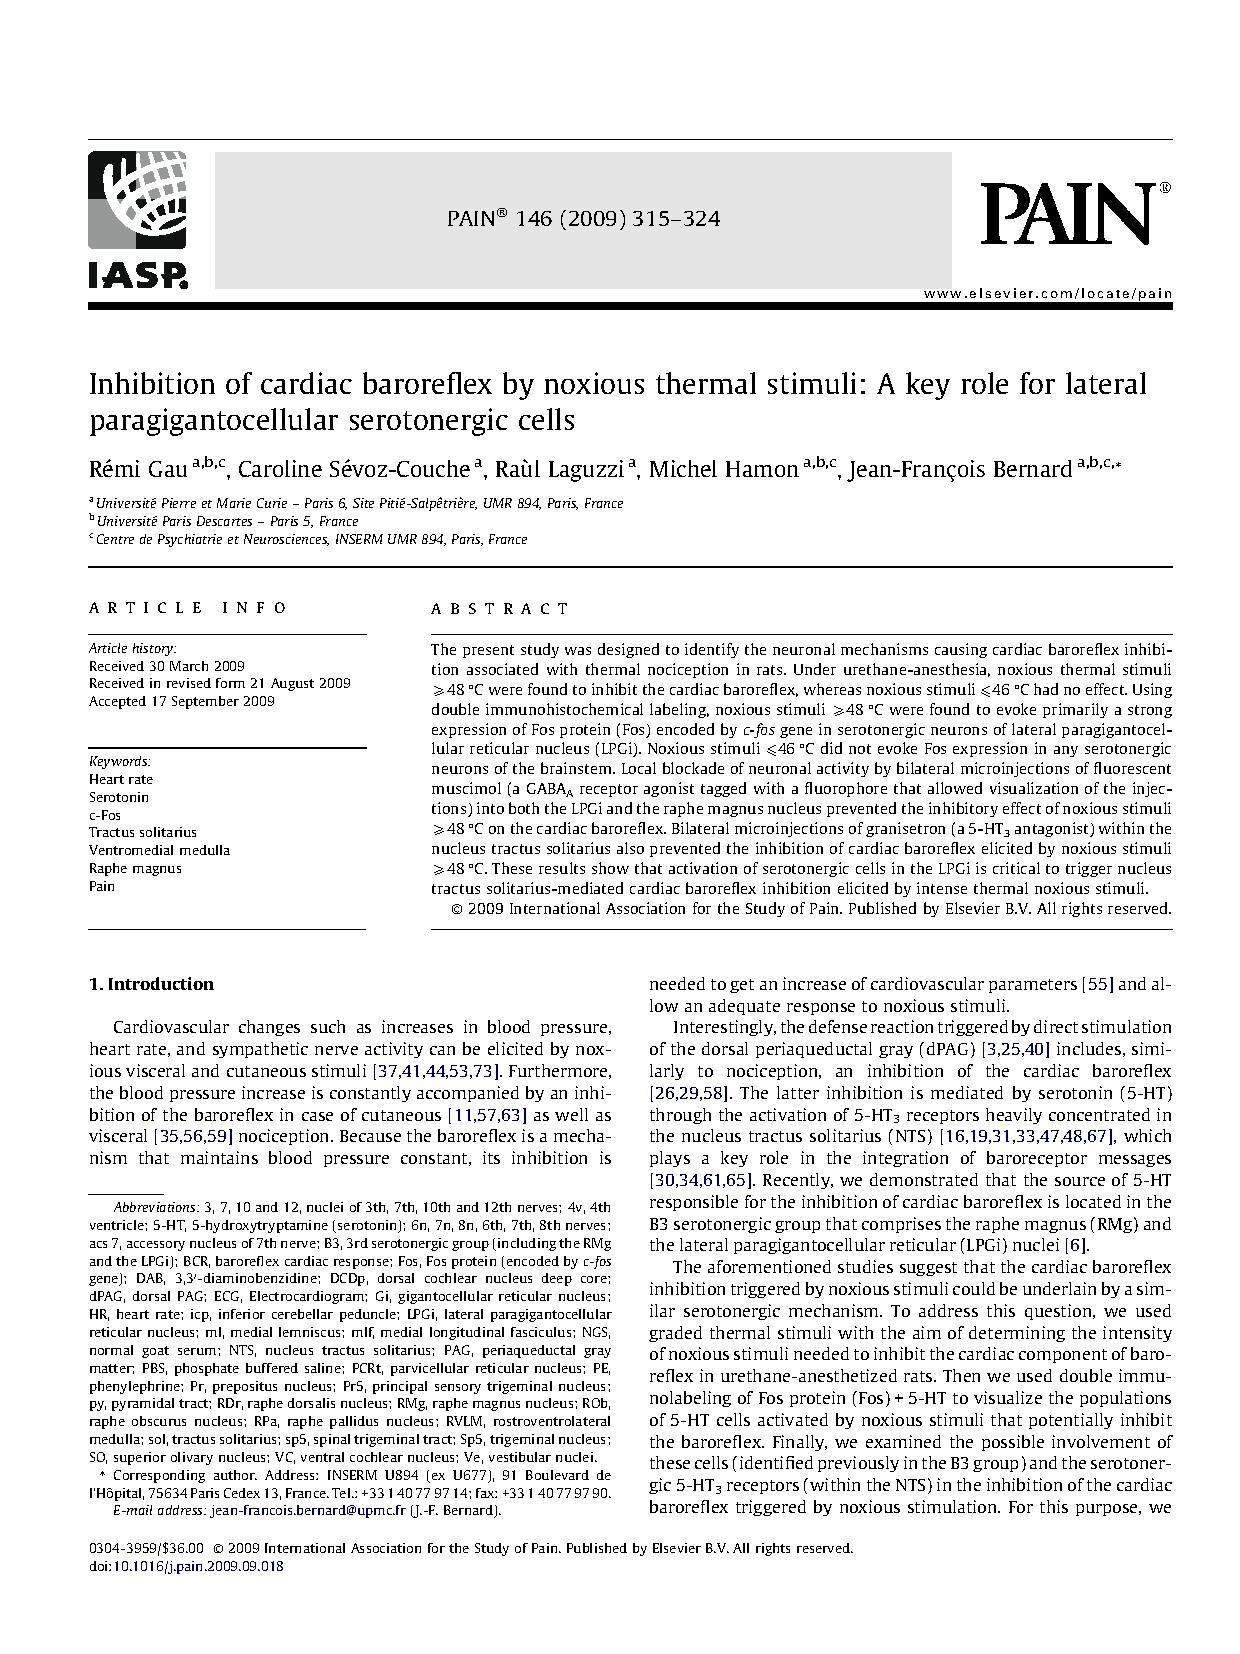
\includepdf[pages={1-10}]{2009Gau.pdf}

\cleardoublepage

\begin{figure}[p]

\begin{center}
 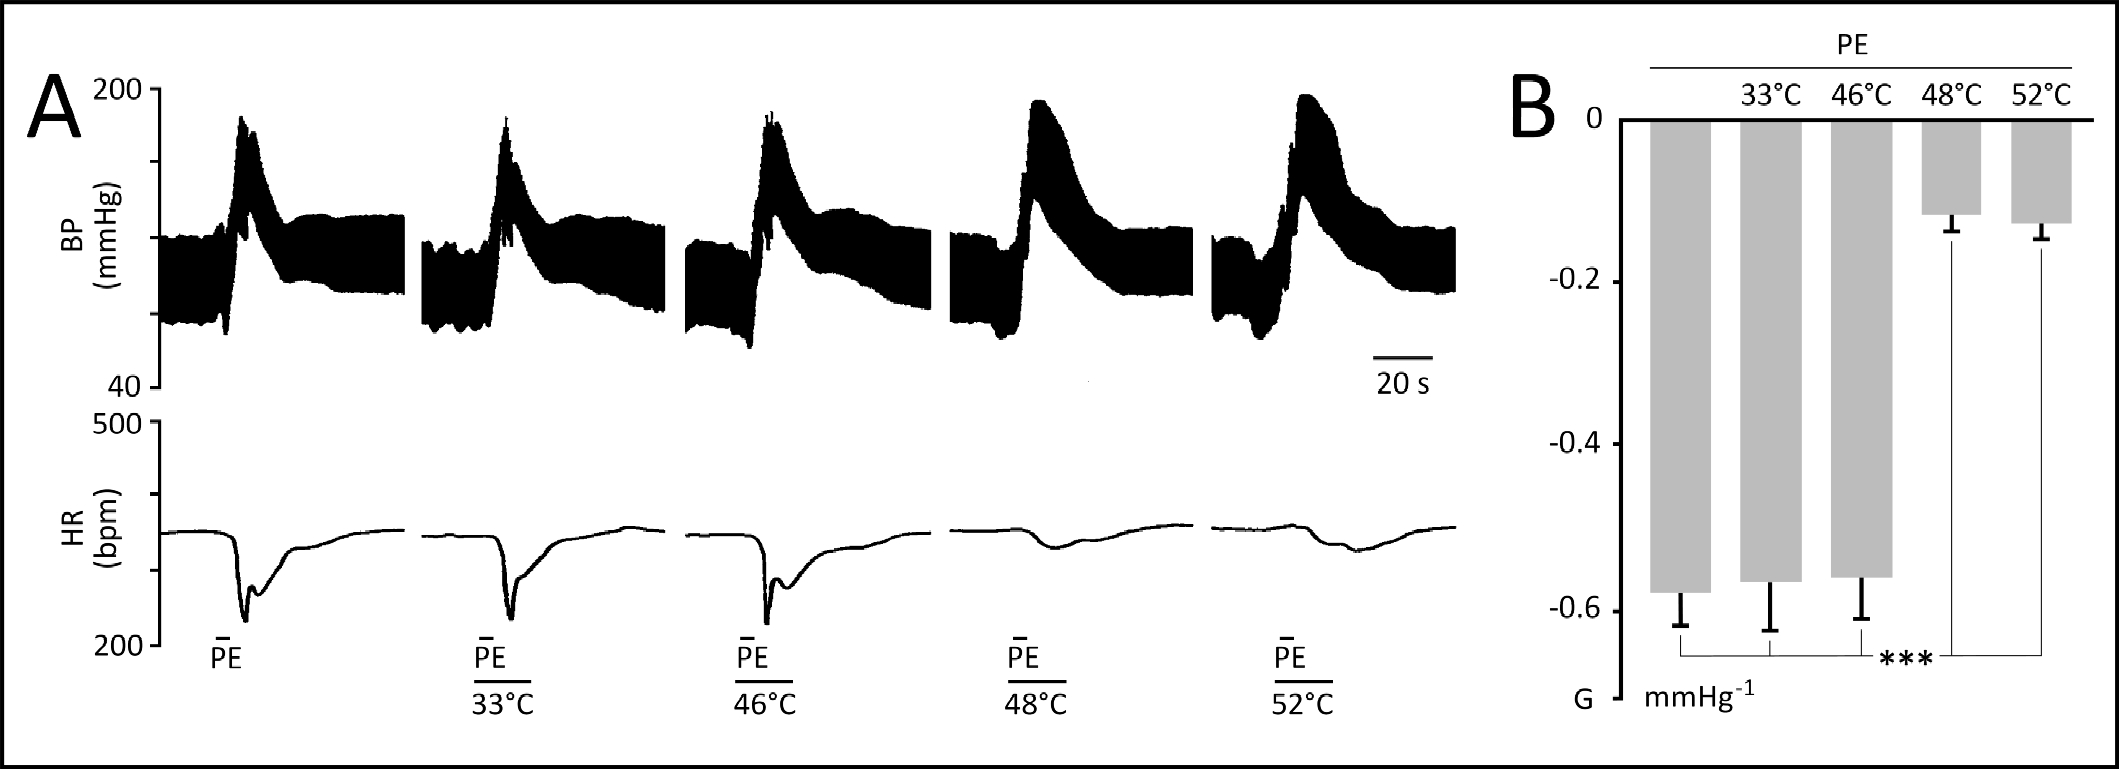
\includegraphics[scale=1]{Article2-FIG1.jpg} 
\end{center}

\caption{\textbf{Effects of innocuous and noxious thermal stimuli on baroreflex cardiac responses}}

{\protect\parbox[t]{18cm}{
\begin{small}
\textbf{(A)}: Representative tracings showing the baroreflex bradycardia evoked by intra-arterial phenylephrine (PE) only and by PE during 33, 46, 48, and 52 °C stimulation of the hind paw. Note that the inhibition of baroreflex cardiac response was elicited only by 48 and 52 °C highly nociceptive temperatures.\\
\textbf{(B)}: Histogram of the mean (+S.E.M.) baroreflex gain elicited by PE only (n = 30) and by PE during 33 °C (n = 11), 46 °C (n = 12), 48 °C (n = 13), 52 °C (n = 25) thermal stimuli. Note that the mean gain (G) of baroreflex was clearly unchanged by 33 and 46 °C whereas it was strongly decreased (absolute value) by 48 and 52 °C. Each of PE only, 33, and 46 °C groups was significantly different from each of 48 and 52 °C groups (p < 0.001).\\
BP: blood pressure; G: gain of cardiac baroreflex; HR: heart rate; $***$:p < 0.001.
\end{small}}}

\label{Article2-FIG1}

\end{figure}


\begin{figure}[p]

\begin{center}
 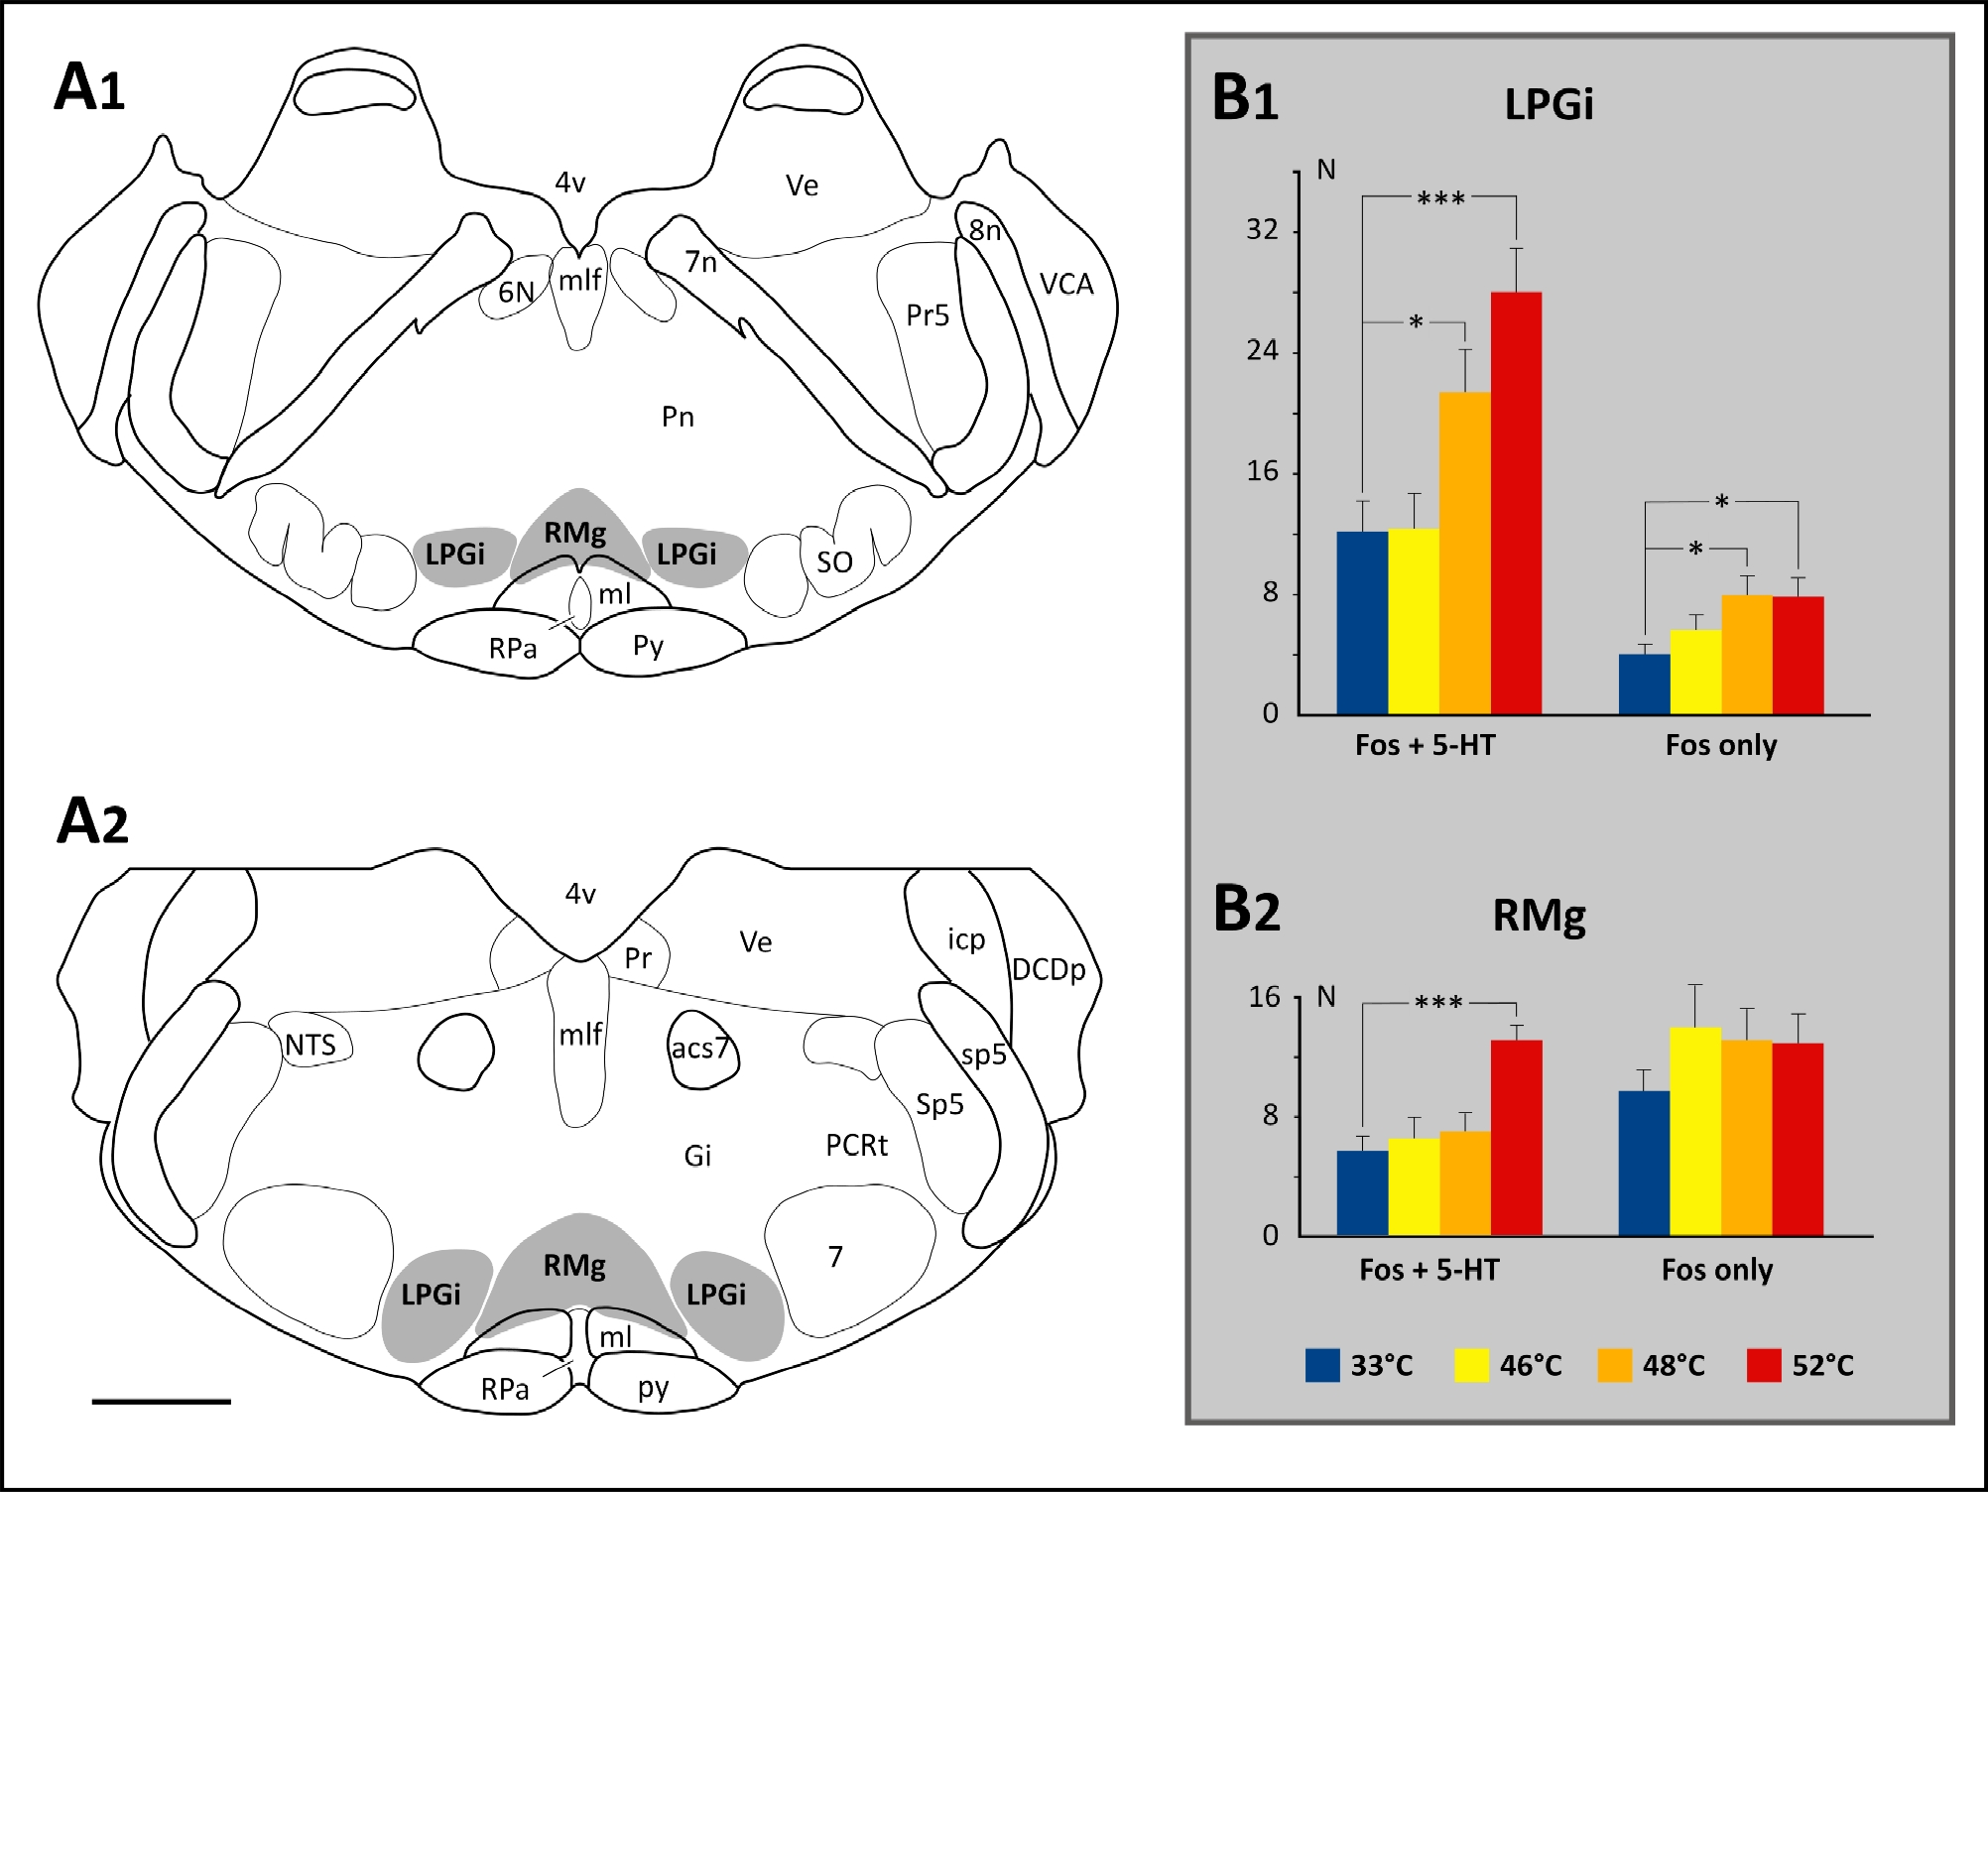
\includegraphics[width=18cm]{Article2-FIG2.jpg} 
\end{center}

\caption{\textbf{Fos expression within B3 region after thermal noxious stimuli}}

{\protect\parbox[t]{18cm}{
\begin{small}
\textbf{(A1–A2)}: Coronal sections of the brainstem at the level of the rostral and the mid portions (bregma -10.2 and -10.9 mm) of B3 serotonergic group (gray area). \\
\textbf{(B1-B2)}: Histograms of the number of serotonergic and non-serotonergic Fos positive cells in both the ipsilateral and contralateral LPGi (B1) and the RMg (B2), within the rostral + mid portion of the B3 region (gray areas in A). \\
Blue, yellow, orange, and red bars indicate the mean (+ S.E.M.) number (N) of Fos expressing cells per section after 33 °C (n = 9), 46 °C (n = 5), 48 °C (n = 5), and 52 °C (n = 10) thermal stimuli, respectively. LPGi: lateral paragigantocellular nucleus; RMg: raphe magnus nucleus; $***$: p < 0.001, $*$: p < 0.05. Abbreviations in A1, A2: see list in article. Scale bar = 1 mm.
\end{small}}}

\label{Article2-FIG2}

\end{figure}


\begin{figure}[p]

\begin{center}
 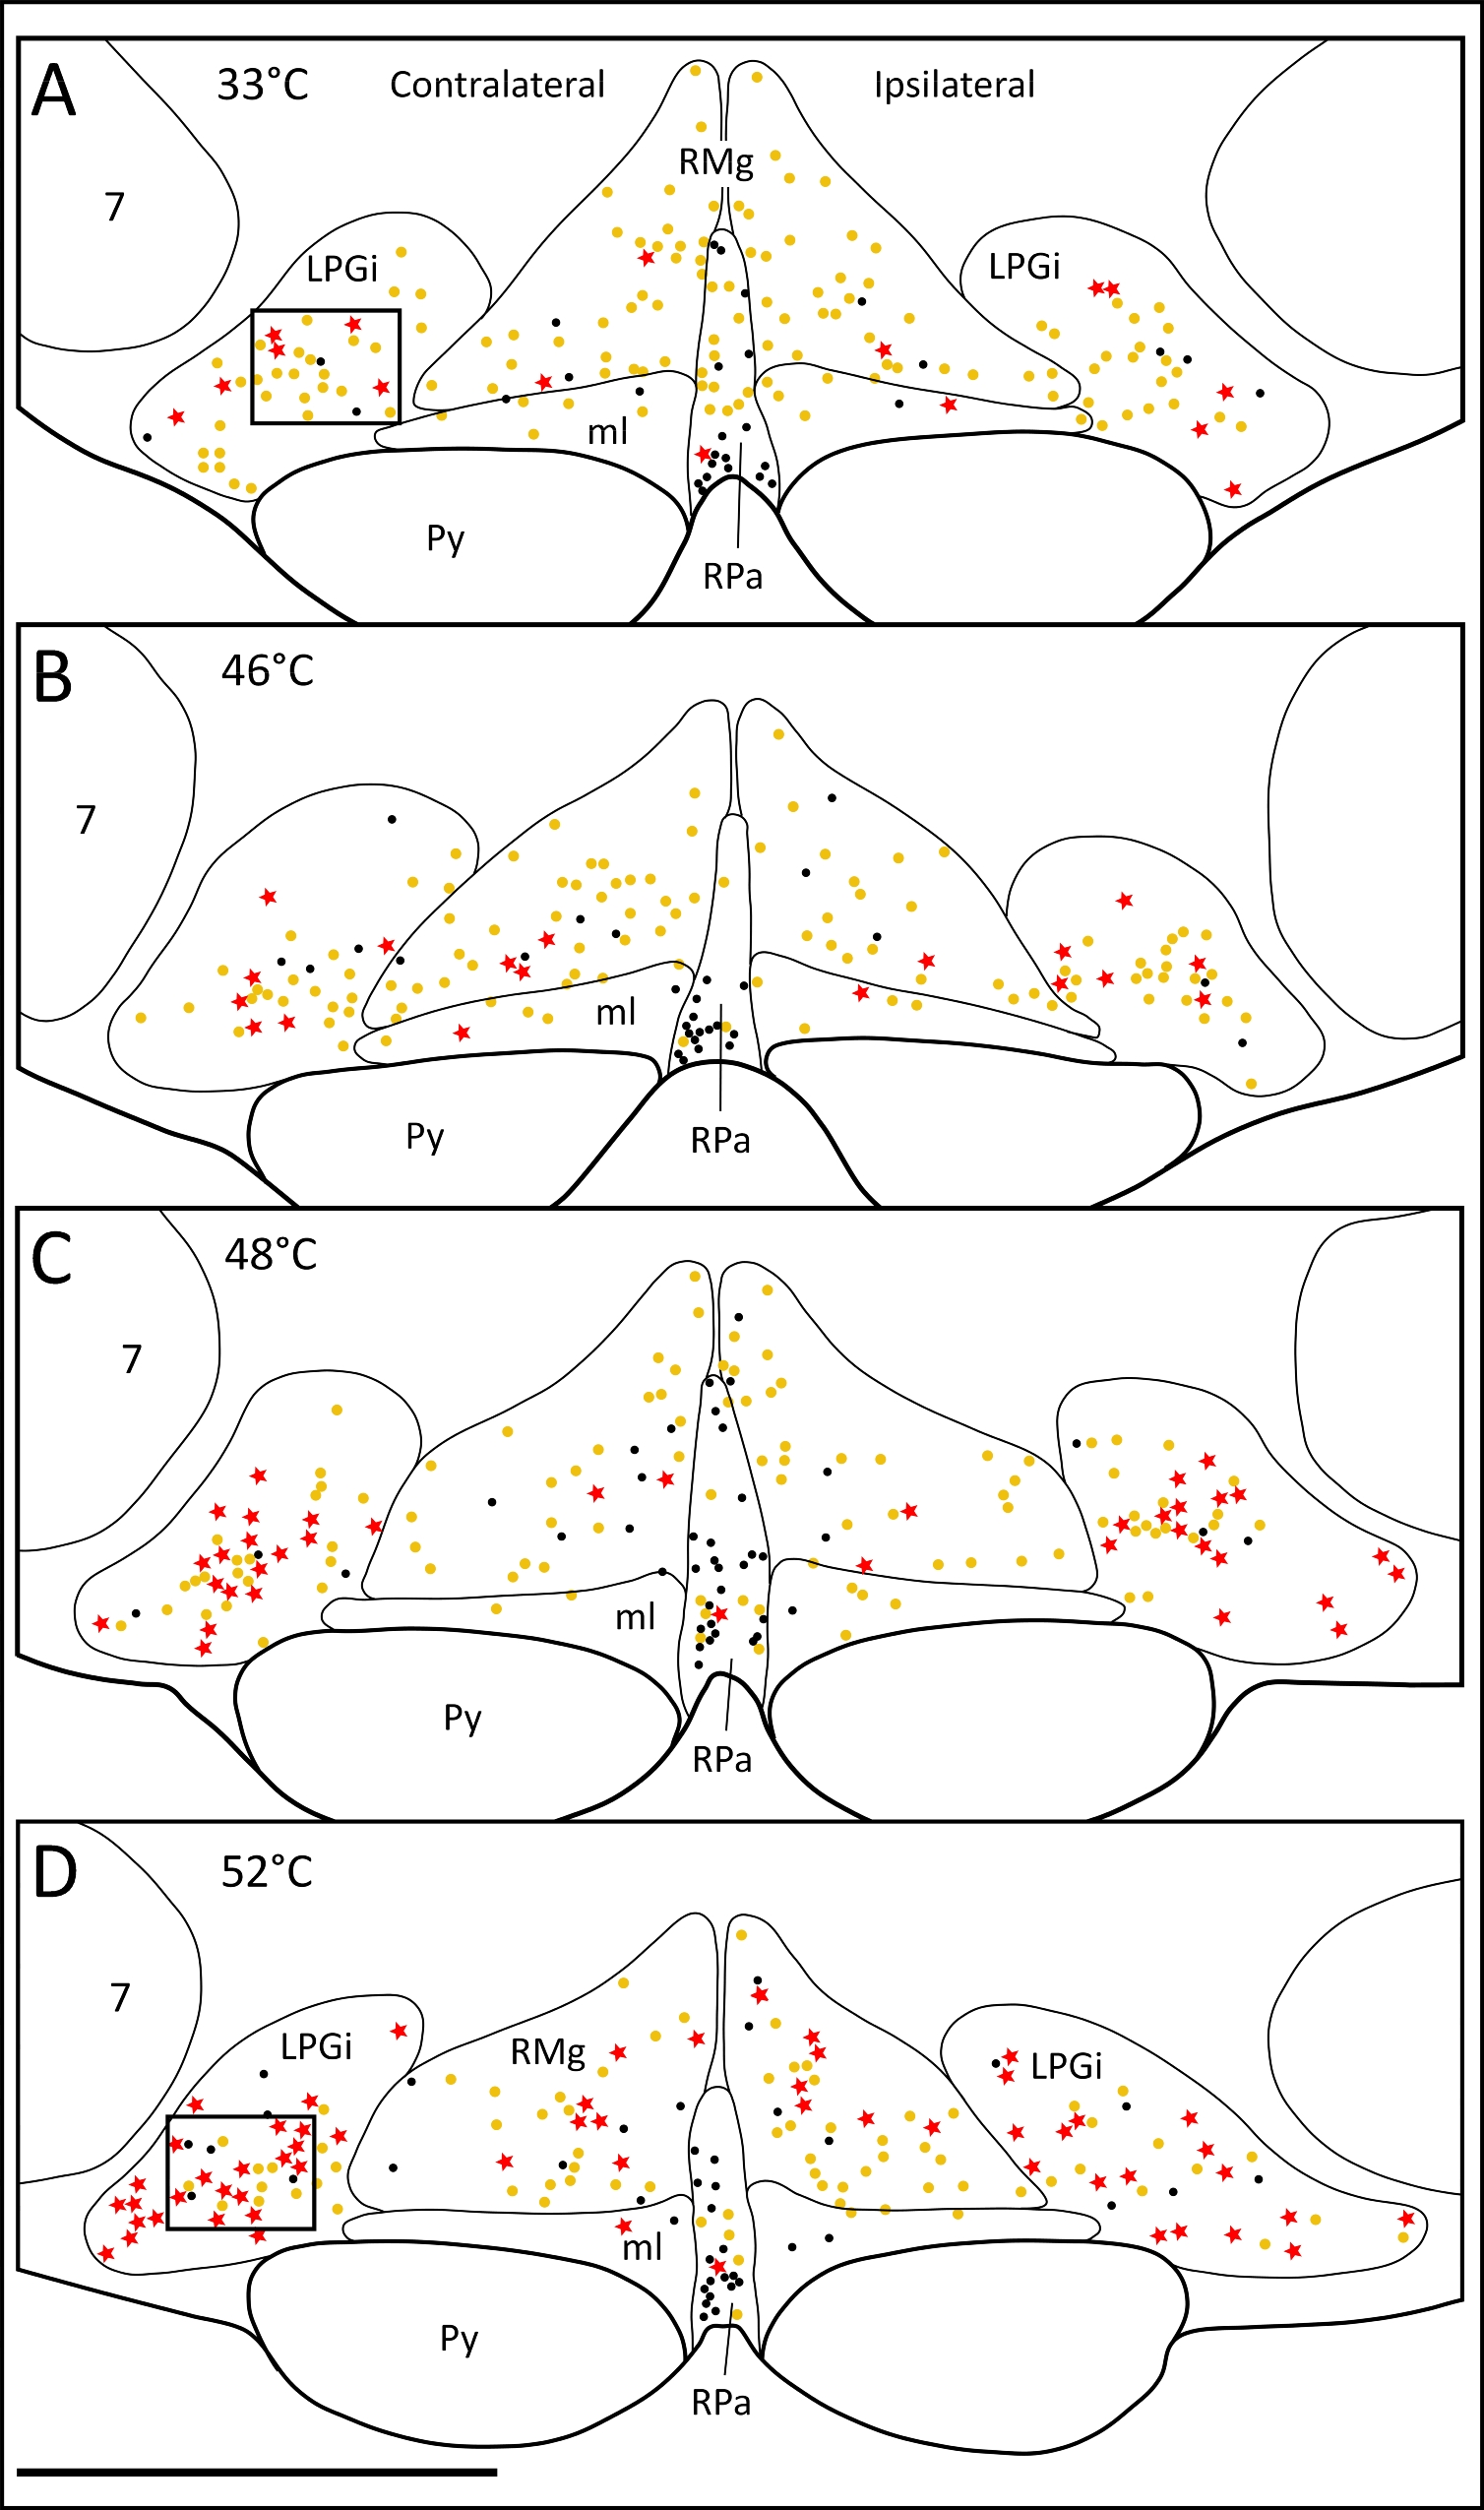
\includegraphics[scale=0.9]{Article2-FIG3.jpg} 
\end{center}

\caption{\textbf{Distribution of labeled neurons in the mid-rostrocaudal extent of the B3 region}}

{\protect\parbox[t]{18cm}{
\begin{small}
\textbf{(A–D)}: Camera lucida drawings of coronal sections at Bregma level = -10.9 mm for rats whose right hind paw was dipped into water bath at 33, 46, 48, and 52 °C, respectively.\\
Each drawing depicts neurons expressing (1) both Fos and 5-HT (red star), (2) only 5-HT (brown/yellow circle) or (3) only Fos (small black point). The framed areas in (A) and (D), in the contralateral LPGi, indicate the location of the high magnification microphotographs of Fig. 4A and B.\\
Note the increased density of double-labeled neurons and the decreased density of single 5-HT labeled neurons in (D) compared to (A).\\
Ipsilateral, Contralateral: side ipsilateral, contralateral to stimulated paw. Abbreviations: see list. Scale bar = 1 mm.
\end{small}}}

\label{Article2-FIG3}

\end{figure}


\begin{figure}[p]

\begin{center}
 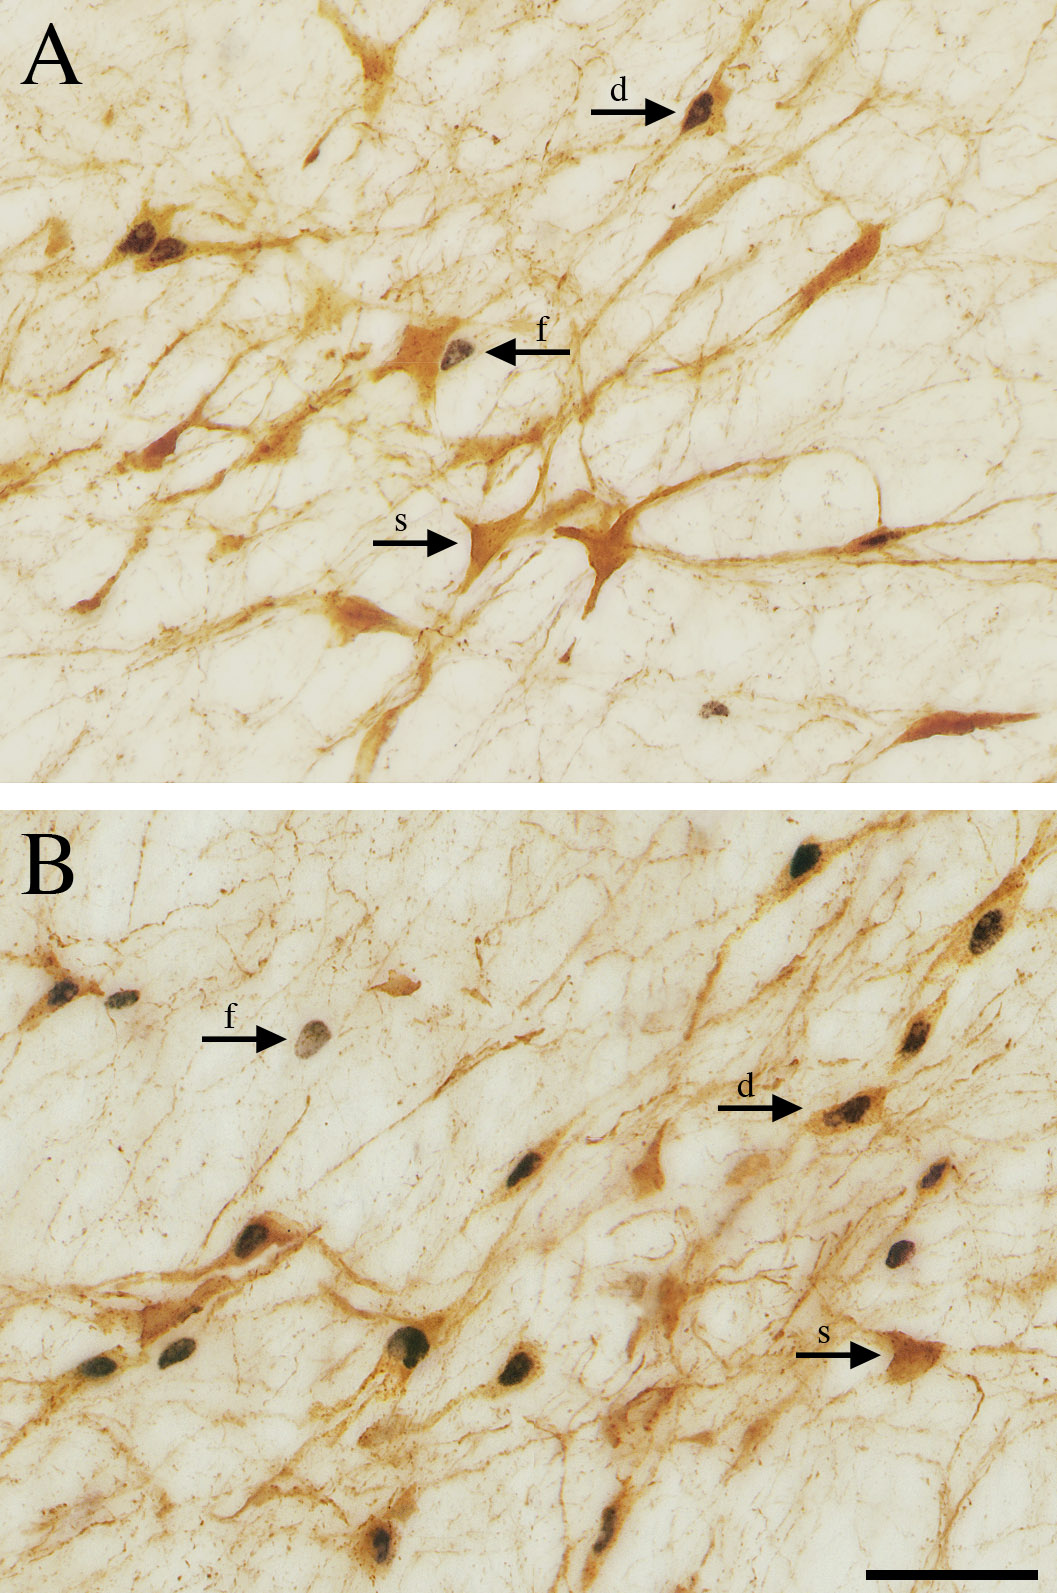
\includegraphics[scale=1.5]{Article2-FIG4.jpg} 
\end{center}

\caption{\textbf{Color digitized photomicrographs of labeled neurons in the B3 region}}

{\protect\parbox[t]{18cm}{
\begin{small}
\textbf{(A) and (B)}: photomicrographs of the lateral paragigantocellular (LPGi) regions framed in Figure 3 A and D, respectively. (A) 33 °C Stimulated animal. (B) 52 °C Stimulated animal. Note the strong increase of Fos + 5-HT double-labeled neurons in (B) compared to (A).\\
Arrows with d, s and f indicate examples of Fos + 5-HT double-labeled (black core surrounded by brown staining), 5-HT single-labeled (cytoplasm brown staining) and Fos single-labeled (nucleus black staining) neurons, respectively. Scale bar = 50 µm.
\end{small}}}

\label{Article2-FIG4}

\end{figure}


\begin{figure}[p]

\begin{center}
 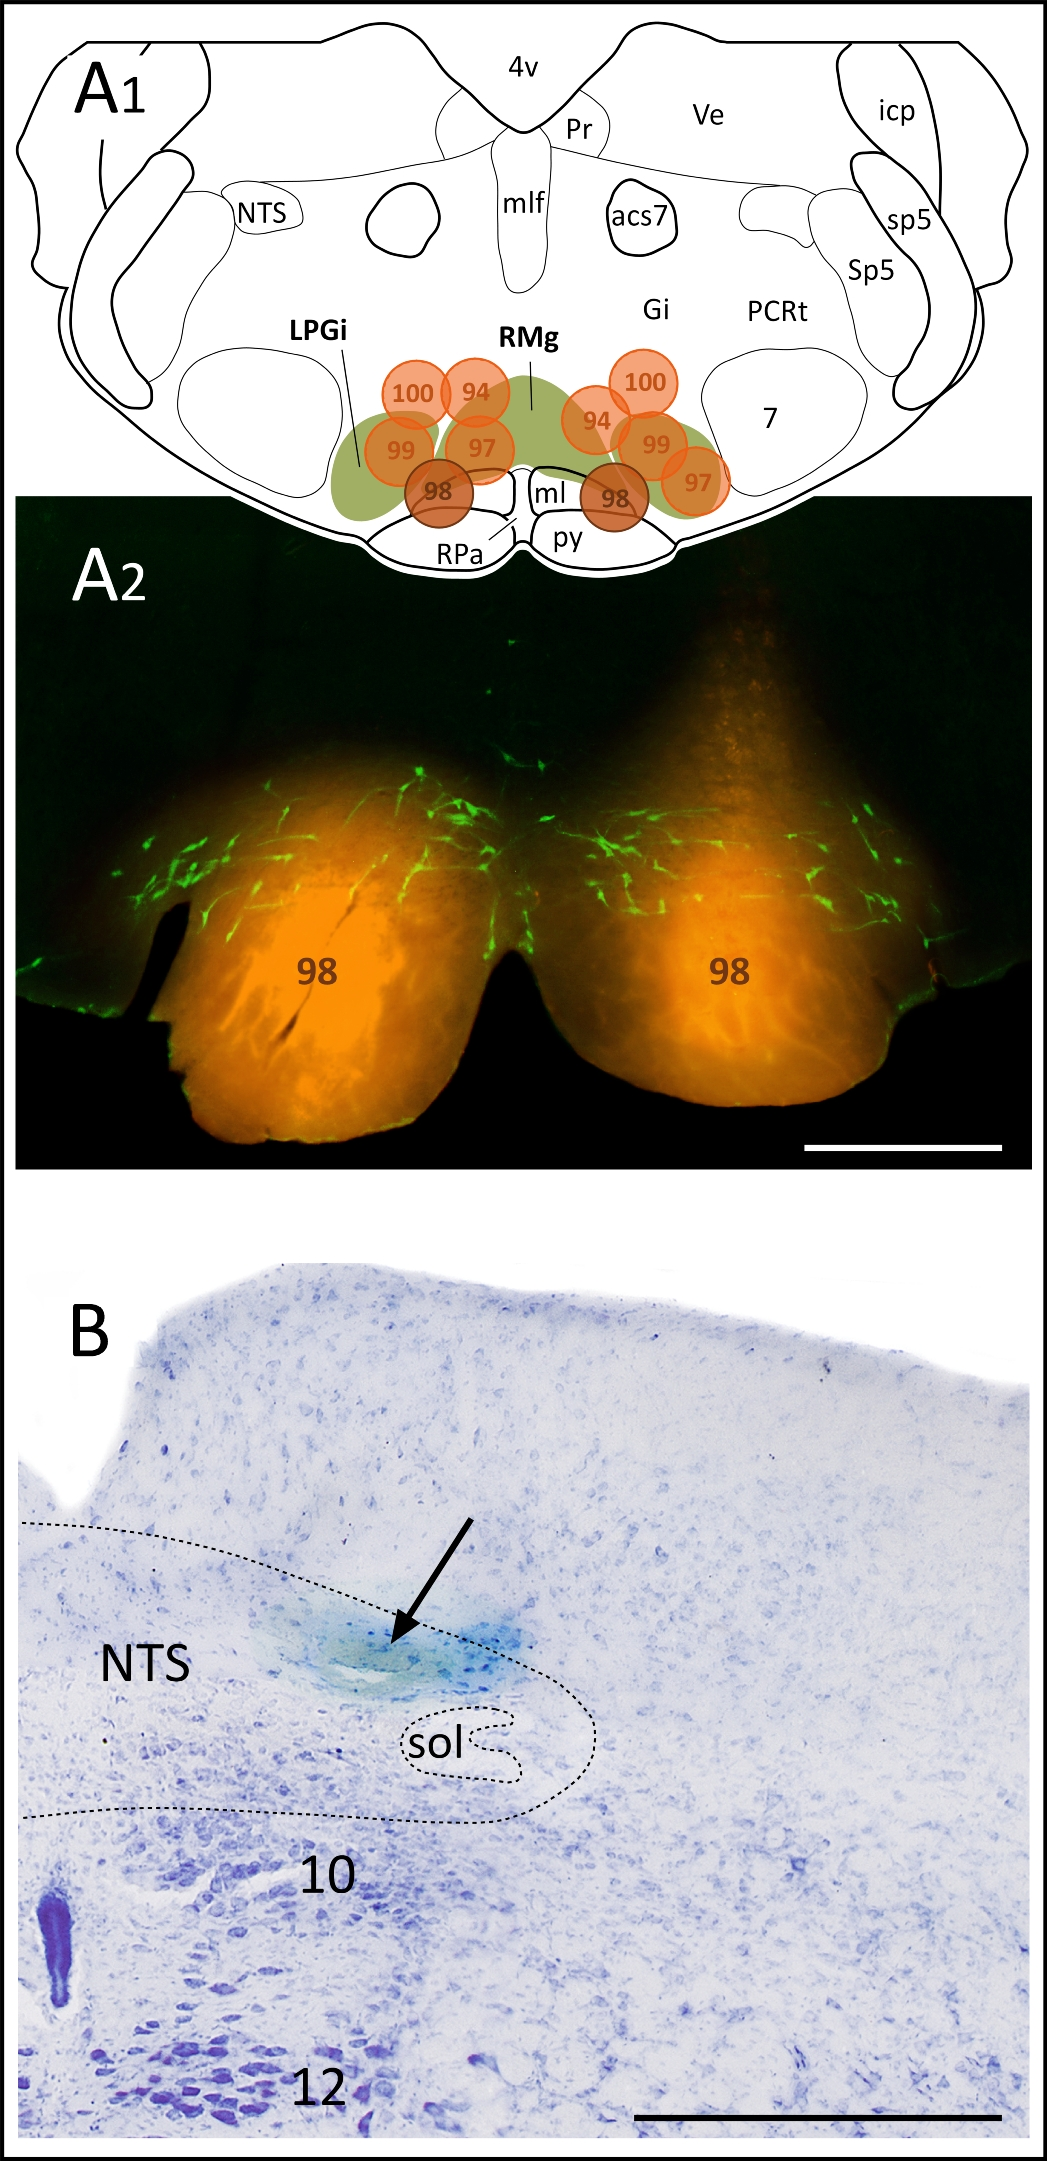
\includegraphics[scale=1.1]{Article2-FIG5.jpg} 
\end{center}

\caption[Microinjection sites localisation in the B3 group and the NTS]{\textbf{Microinjection sites of bodypi muscimol in the B3 group and pontamine blue dye in the NTS}}

{\protect\parbox[t]{18cm}{
\begin{small}
\textbf{(A1)}: Coronal section at the level of B3 group (green) showing bilateral bodipy muscimol microinjections. Each couple of bilateral microinjections, in a given animal, was identified by the same number in two orange circles.\\
\textbf{(A2)}: Photomicrograph showing typical case (No. 98) of bilateral microinjections of bodipy muscimol (orange fluorescence) within the serotonergic neuron area (green) of the B3 group (comprising the RMg and the LPGi; Bregma: -11 mm). 
\textbf{(B)}: Photomicrograph showing pontamine blue deposit (arrow) around the tip of the micropipette used to inject granisetron into the NTS (Bregma: -13.5 mm).\\
Abbreviations: see list. Scale bars = 500 µm (A2 and B).
\end{small}}}

\label{Article2-FIG5}

\end{figure}


\begin{figure}[p]

\begin{center}
 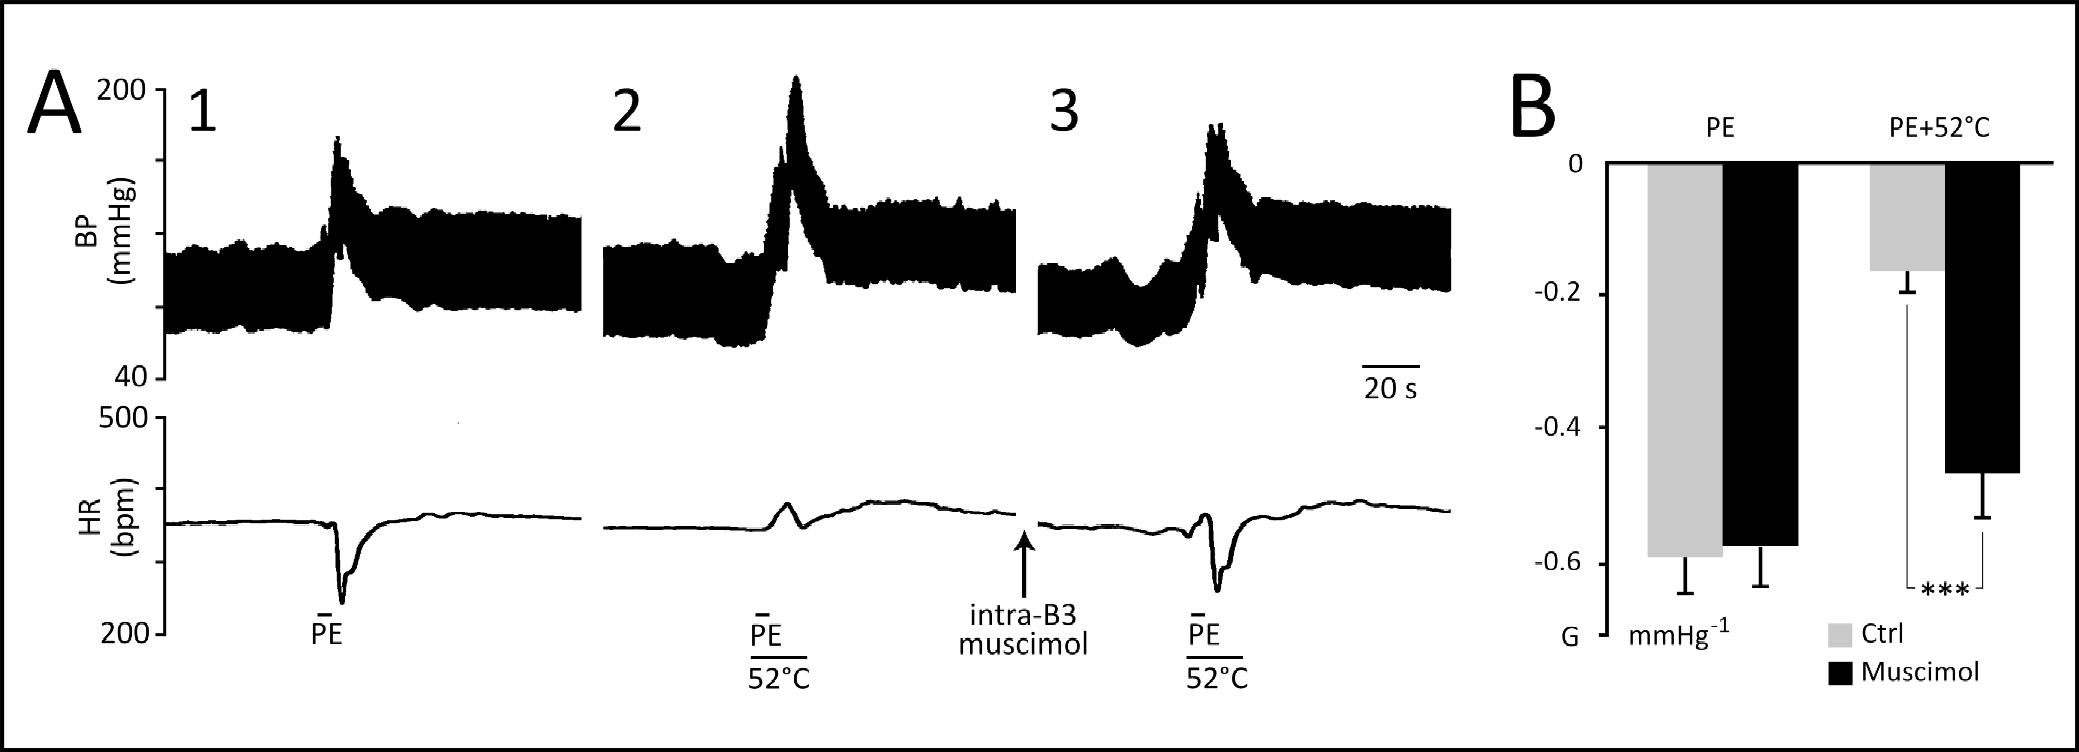
\includegraphics[scale=1]{Article2-FIG6.jpg} 
\end{center}

\caption[Effects of intra-B3 muscimol microinjection on the baroreflex inhibition]{\textbf{Effects of muscimol microinjection into the B3 region upon the baroreflex inhibition by noxious thermal stimuli}}

{\protect\parbox[t]{18cm}{
\begin{small}
\textbf{(A)}: Representative tracings showing, in the same animal, (1) the baroreflex bradycardia evoked by PE, (2) the inhibition of the baroreflex by 52 °C noxious stimulus, and (3) the full prevention of the latter inhibition by prior bilateral microinjections of fluorescent muscimol (5 mM) into the B3 region (injection No. 98 shown in Fig. 5).\\ 
\textbf{(B)}: Histogram of the mean (+S.E.M.) baroreflex gain elicited by PE only (PE) and by PE during 52 °C noxious stimulation (PE + 52 °C), before (gray) and after (black) muscimol microinjection into the B3 region (each bar: n = 15).\\ 
Note that the mean baroreflex gain elicited by PE only was clearly unchanged by muscimol, whereas the strong decrease in baroreflex gain elicited by 52 °C noxious stimulation was markedly reduced by intra-B3 muscimol.\\ 
BP: blood pressure; G: gain of cardiac baroreflex; HR: heart rate; $***$: p < 0.001.
\end{small}}}

\label{Article2-FIG6}

\end{figure}


\begin{figure}[p]

\begin{center}
 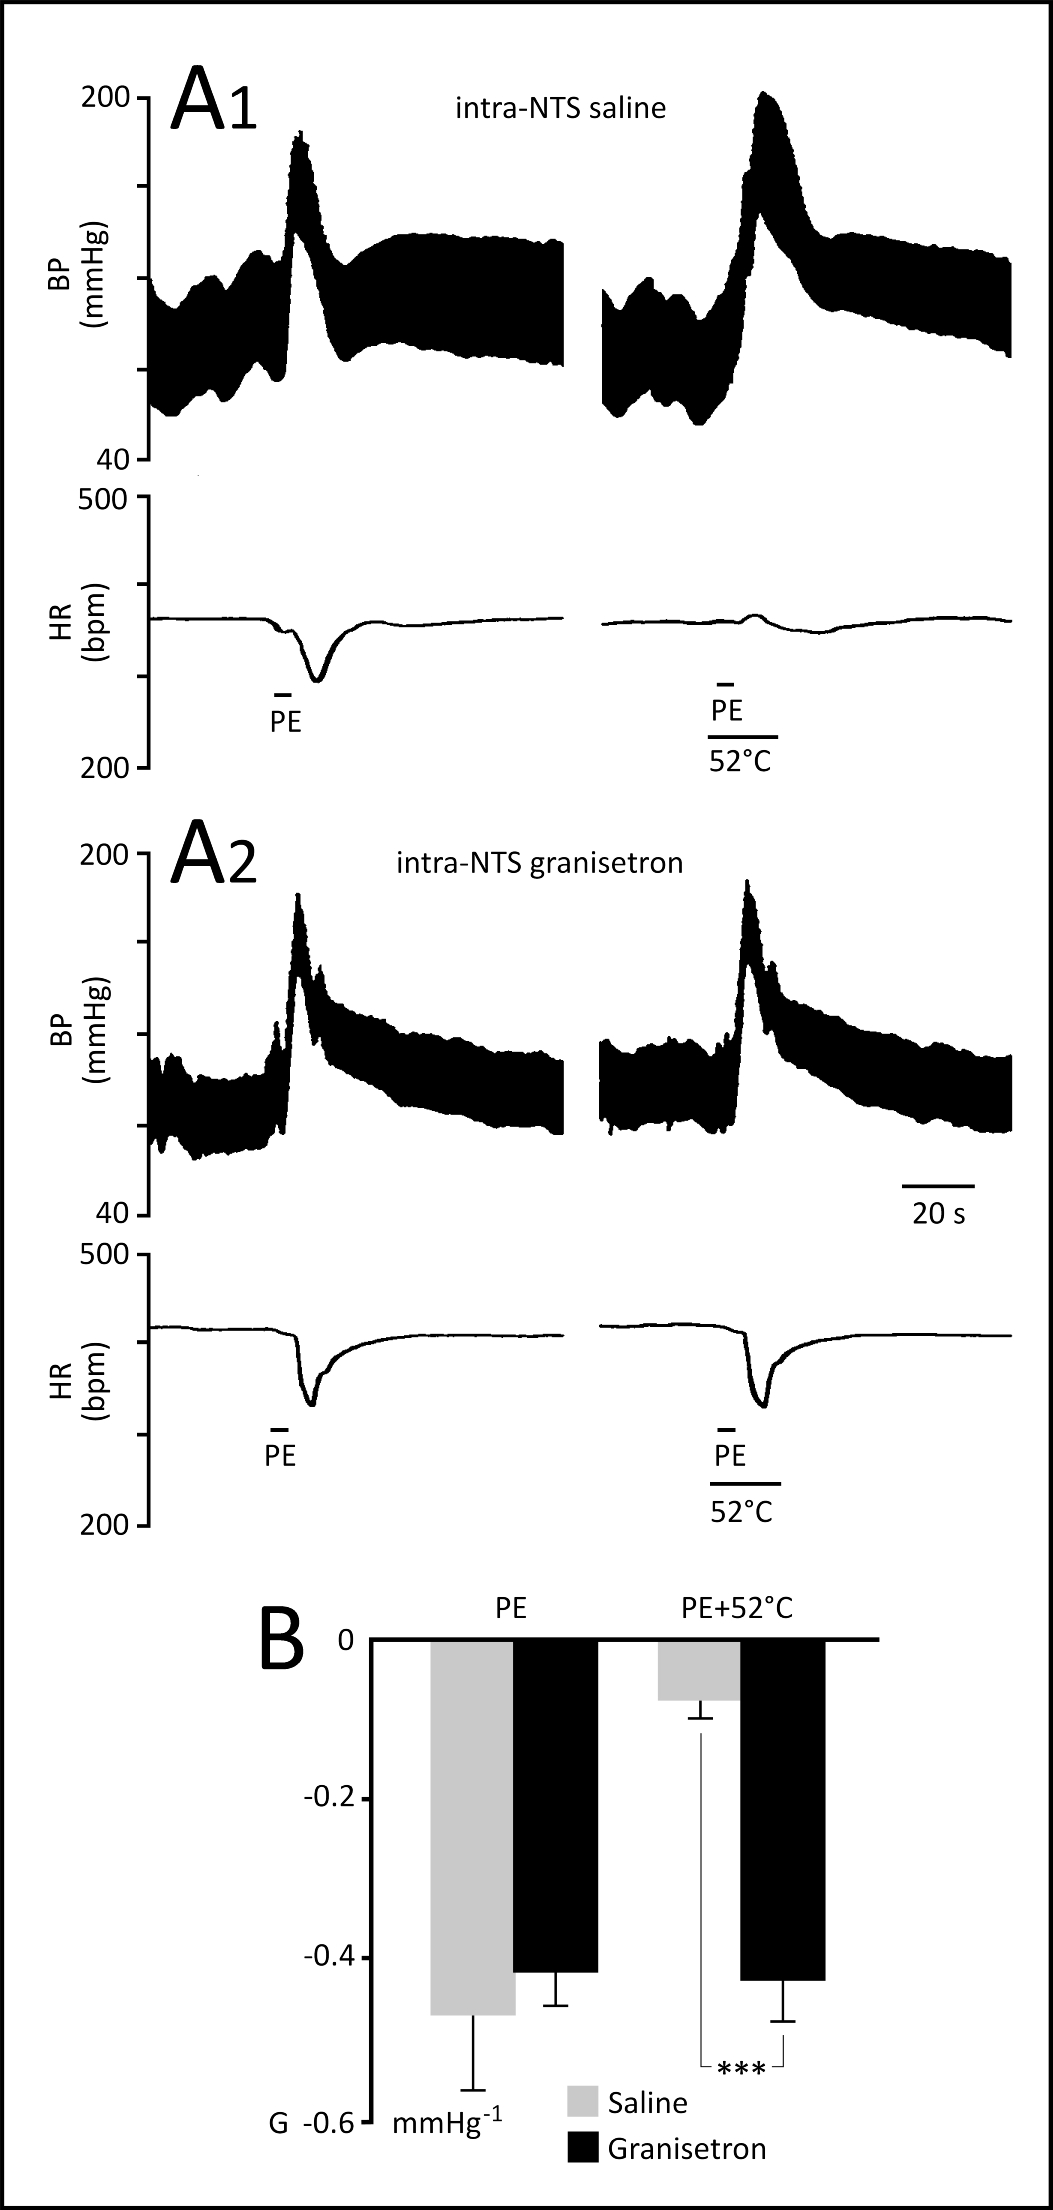
\includegraphics[scale=1]{Article2-FIG7.jpg} 
\end{center}

\caption[Effects of intra-NTS granisetron microinjection on the baroreflex inhibition]{\textbf{Effects of granisetron microinjection into the NTS upon the baroreflex inhibition by noxious thermal stimuli}}

{\protect\parbox[t]{18cm}{
\begin{small}
\textbf{(A1)}: In control conditions, the tracing shows that PE-evoked baroreflex bradycardia and that concomitant 52 °C thermal noxious stimulation inhibited this response.\\ 
\textbf{(A2)}: After granisetron microinjections into the NTS, the tracing shows that PE-evoked baroreflex bradycardia persisted during 52 °C noxious stimulation.\\ 
\textbf{(B)}: Histogram of the mean (+S.E.M.) baroreflex gain elicited by PE only (PE) and by PE during 52 °C noxious stimulation (PE + 52 °C), after saline (gray, each bar: n = 5) or granisetron (black, each bar: n = 7) microinjection into the NTS.\\ 
Note that the mean baroreflex gain by PE only was clearly unchanged by granisetron, whereas the strong decrease of baroreflex gain elicited by 52 °C noxious stimulus was markedly prevented by intra-NTS granisetron.\\ 
BP: blood pressure; G: gain of cardiac baroreflex; HR: heart rate; $***$: p < 0.001.
\end{small}}}

\label{Article2-FIG7}

\end{figure}

\cleardoublepage

\section{RÉSULTATS SUPPLÉMENTAIRES}

\subsection{Introduction}

Les effets d’une stimulation nociceptive cutanée sur la pression artérielle et la fréquence cardiaque sont généralement intenses. Toutefois, les stimuli nociceptifs n’inhibant que la composante parasympathique du baroréflexe (Pickering et al. 2003), il est nécessaire de bloquer les effets sympathiques au niveau cardiaque (i.e. tachycardie) pour pouvoir quantifier la bradycardie du baroréflexe. Pour ce faire, on utilise un $\beta$ bloquant (dans ce cas l’aténolol) qui diminue la réponse cardiaque sympathique sans affecter la réponse pressive médiée par des récepteurs adrénergiques $\alpha$.

Les détails des effets de stimuli nociceptifs thermiques sur la pression artérielle, la fréquence cardiaque ainsi que les effets de l’aténolol sont décrits ci-dessous.

\subsection{Résultats}

\subsubsection{Effets de la stimulation nociceptive thermique sur la pression artérielle}

Les effets de la nociception sur la pression artérielle ont été évalués des rats anesthésiés à l’uréthane (n = 7). \textbf{La réponse de la pression artérielle à des stimulations nociceptives est de type « tout ou rien » : des stimulations thermiques inférieures ou égales à 46 °C n’avaient pas d’effet sur la pression artérielle moyenne, alors que toutes les stimulations nociceptives supérieures à 46 °C augmentaient la pression artérielle de façon similaire.} De tels stimuli, appliqués au niveau de la patte, augmentaient la pression artérielle en moyenne de 36 $\pm$ 4 mmHg à partir d'une pression artérielle de base de 90 $\pm$ 5 mmHg (soit une augmentation de 39 $\pm$ 6 \%) (voir Figure \ref{Figure 11} A1-2 et B - page \pageref{Figure 11}). Cette élévation de la pression artérielle débutait 2 à 5 s après l'application de la température nociceptive et atteignait son maximum 10 à 15 s plus tard. Elle demeurait stable jusqu'à la fin de la stimulation. Le retour au niveau basal se faisait progressivement en une à deux minutes. Pour toutes les températures testées supérieures à 46°C, les variations observées étaient quasi-similaires. Dans nos conditions, des températures au seuil de la nociception (44°C) ou clairement nociceptives, jusqu'à 46°C, ne provoquaient aucune modification de la pression artérielle (voir Figure \ref{Figure 11} A1-2 et B - page \pageref{Figure 11}). Ainsi l'augmentation de la pression artérielle semble être une réponse qui ne code pas l'intensité de la stimulation ; elle apparait d'emblée à son maximum pour une température de 48°C, considérée généralement comme le seuil de la douleur intolérable.

\subsubsection{Effets de la stimulation nociceptive thermique sur la fréquence cardiaque}

\textbf{Comme la pression artérielle, la fréquence cardiaque était fortement augmentée par une température franchement nociceptive (voir Figure \ref{Figure 11} A3 et B - page \pageref{Figure 11})}. La fréquence cardiaque augmentait en moyenne de 100 $\pm$ 11 bpm à partir d'une fréquence de base de 283 $\pm$ 12 bpm (soit une augmentation de 42 $\pm$ 5 \%). Comme l’élévation de la pression artérielle, l'augmentation de la fréquence cardiaque évoluait peu (de + 26 \% à + 31 \%) en fonction de l'intensité du stimulus nociceptif entre 48°C et 52°C. En revanche, la fréquence cardiaque n’était quasiment pas modifiée par les températures nociceptives d'intensité moyenne, entre 44°C et 46°C (voir Figure \ref{Figure 11} A3 et B - page \pageref{Figure 11}).

\subsubsection{Quantification de l'action de l’aténolol}

L’aténolol (un antagoniste des récepteurs adrénergiques $\beta_{1}$ et $\beta_{2}$) a été utilisé pour supprimer la composante cardiaque sympathique (tachycardie) induite par une stimulation nociceptive, et ne laisser que la composante parasympathique cardiaque du baroréflexe. Nous avons donc évalué les effets de l’aténolol sur les différents paramètres cardiovasculaires mesurés.

L’administration d’aténolol n’a aucun effet sur les valeurs au repos des paramètres cardiovasculaires. Chez les rats traités, la pression artérielle était de 83 $\pm$ 2 mmHg et la fréquence cardiaque de 296 $\pm$ 16 bpm, c'est-à-dire similaires à celles observées chez les rats contrôles. L’aténolol n'a que peu d'effet sur l'augmentation de pression artérielle déclenchée par un stimulus nociceptif thermique. En revanche, comme attendu, l’aténolol réduit fortement la tachycardie induite par un même stimulus. Une réponse résiduelle faible persistait cependant pour les températures les plus élevées (voir Figure \ref{Figure 11} C et D - page \pageref{Figure 11}) : elle était d'environ + 8 \% (soit + 23 $\pm$ 5 bpm) pour des températures allant de 48°C à 52°C. 

En pratique, une telle variation n'est pas gênante pour observer les variations de la bradycardie du baroréflexe qui sont nettement plus fortes (> 120 bpm ; Article 2 Figure 1 A – page \pageref{Article2-FIG1}).

\begin{figure}[p]

\begin{center}
 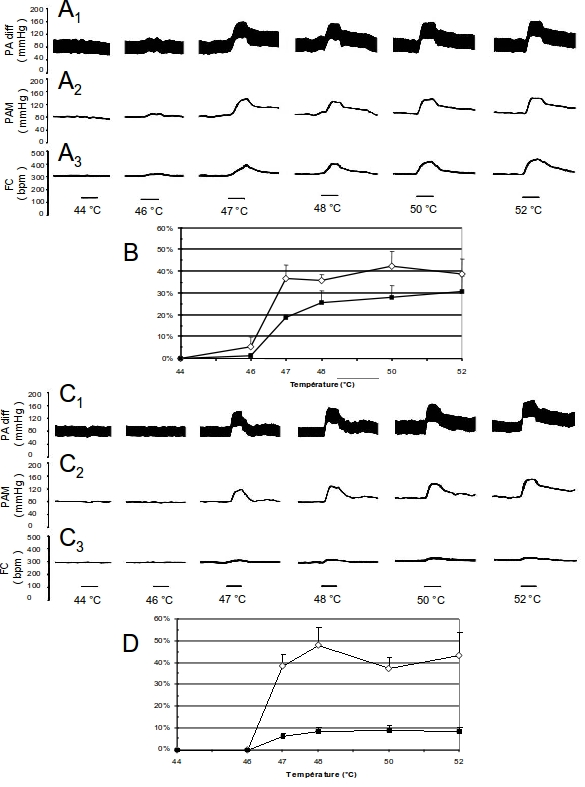
\includegraphics[width=14.5cm]{Figure11.jpg} 
\end{center}

\caption{\textbf{Modifications des paramètres cardiovasculaires par des stimuli nociceptifs thermiques}}

{\protect\parbox[t]{18cm}{
\begin{small}
A) Pression artérielle instantanée (A1 - PA diff), moyenne (A2 - PAM) et fréquence cardiaque (A3 - FC) observées lors de l'application de stimuli thermiques cutanés (barres, 30 s) d’intensités croissantes (44 à 52~°C).\\
B) Augmentation moyenne (en pourcentage du niveau de base $\pm$ SEM) de la pression artérielle (losanges blancs) et de la fréquence cardiaque (carrés noirs) en fonction des stimuli thermiques (44 à 52~°C). \\
C) Pression artérielle instantanée (C1 - PA diff), moyenne (C2 - PAM) et fréquence cardiaque (C3 - FC) observées lors de l'application de stimulus thermiques cutanés (barres, 30 s) d’intensités croissantes (44 à 52~°C) dans le cas d'un animal prétraité à l’aténolol.\\
D) Augmentation moyenne (en pourcentage du niveau de base $\pm$ SEM) de la pression artérielle (losanges blancs) et de la fréquence cardiaque (carrés noirs) en fonction des stimuli thermiques (44 à 52~°C).
\end{small}}}

\label{Figure 11}

\end{figure}

\begin{sidewaystable}
% \documentclass[a4paper,12pt,twoside]{report}
% 
% % Pour inclure des pages issus d'un autre pdf
% \usepackage{pdfpages}
% 
% 
% \usepackage[utf8x]{inputenc}
% %\usepackage[latin1]{inputenc}
% \usepackage[T1]{fontenc}
% \usepackage[francais]{babel}
% 
% %\usepackage{layout}
% \usepackage{geometry}
% \geometry{%
% a4paper,
% body={180mm,265mm},
% left=20mm,top=15mm,
% headheight=7mm,headsep=4mm,
% marginparsep=4mm,
% marginparwidth=11mm}
% 
% \usepackage{setspace} % Interligne
% %\singlespacing
% %\onehalfspacing
% \doublespacing
% 
% \setlength{\parindent}{1cm} %Pour le retrait du paragraphe
% 
% \usepackage{soul} % Pour souligner ou barrer du texte
% \usepackage{ulem}
% 
% \usepackage{textcomp}
% 
% %\usepackage{eurosym}
% 
% %\usepackage{bookman} % Différents packs de police
% %\usepackage{charter}
% %\usepackage{newcent}
% %\usepackage{lmodern}
% %\usepackage{mathpazo}
% %\usepackage{mathptmx}
% 
% %\usepackage{url}
% 
% %\usepackage{verbatim}
% 
% %\usepackage{moreverb}
% 
% %\usepackage{listings}
% 
% \usepackage{fancyhdr} % en tête et pied de pages
% 
% \usepackage{wrapfig} % pour encadrer les figures avec du texte
% \usepackage{graphicx}
% 
% \usepackage{multicol} % Pour utiliser l'environnement multicol
% \setlength\columnseprule{.4pt} % Pour mettre un trait séparateur de colonnes\usepackage{multirow} % Pour fusionner les lignes dans les tableaux
% 
% 
% 
% \usepackage{array} % Pour centrer les lignes en hauteur dans un tableau
% \usepackage{rotating} % Pour tourner un tableau
% 
% \usepackage[table]{xcolor} %Pour colorer des cellules
% 
% \usepackage{xcolor}
% \usepackage{colortbl}
% 
% \usepackage{amsmath}
% \usepackage{amssymb}
% \usepackage{mathrsfs}
% 
% %\usepackage{asmthm}
% %\usepackage{makeidx}
% 
% \ifpdf %Pour mettre des hyperliens dans les pdfs
% \usepackage[pdftex=true,
% hyperindex=true,
% colorlinks=true]{hyperref}
% \else
% \usepackage[hypertex=true,
% hyperindex=true,
% colorlinks=false]{hyperref}
% \fi

%\begin{document}
% \begin{sidewaystable}
\setlength{\tabcolsep}{1pt}
\centering
\caption{\textbf{Résultats des comptages dans les différentes Raphés bulbaires}}
\setlength\minrowclearance{6pt}

{%
\newcommand{\mc}[3]{\multicolumn{#1}{#2}{#3}}

\newcolumntype{A}{%
>{\columncolor[gray]{.9}}%
c|}

\newcolumntype{B}{%
>{\columncolor[gray]{1}}%
c|}

{\protect\parbox[t]{25cm}{\singlespacing
\begin{small}
\textbf{(A)} Comptage dans la partie rostrale des noyaux du Raphé Magnus (RMg) et Latéral Paragigantocellulaire (LPGi).
\end{small}}}
\begin{scriptsize}
\begin{center}
\begin{tabular}[c]{||BBc|c|c|c|c|c|c|c|c|c|c|c|c|c|c|c||}
\hline\hline
Rostral		&  		& \mc{4}{A}{\textbf{LPGi Gauche}} 										& \mc{4}{A}{\textbf{RMg Gauche}} 								& \mc{4}{A}{\textbf{RMG droit}}									 & \mc{4}{A}{\textbf{LPGi Droit}}										 \\\hline
 		& \textbf{n} 	& \textbf{5-HT} & \textbf{Fos} 			& \textbf{5-HT+Fos} 		& \textbf{\%} 			& \textbf{5-HT} & \textbf{Fos} 	& \textbf{5-HT+Fos} 		& \textbf{\%} 			& \textbf{5-HT} & \textbf{Fos} 	& \textbf{5-HT+Fos} 		 & \textbf{\%} 			 & \textbf{5-HT} & \textbf{Fos} 		  & \textbf{5-HT+Fos} 		  & \textbf{\%} 		 \\\hline
\textbf{33~°C} 	& 9 		& 26 (1,1) 	& 1,9 (0,3)			& 6,3 (1,2) 			& 24 (4,4)			& 32 (1) 	& 4,9 (0,5) 	& 3 (0,5) 			& 9,2 (1,4) 			& 31 (1,4) 	& 4,4 (0,7) 	& 2,6 (0,4) 			 & 8,5 (1,4) 			 & 25 (0,8) 	 & 2,3 (0,4) 			  & 5,9 (0,9) 			  & 23 (3,5)			 \\\hline
\textbf{46~°C} 	& 5 		& 25 (0,6) 	& 2,7 (0,4) 			& 6,9 (1,2) 			& 27 (4,5)			& 30 (1,6) 	& 7,5 (1,4) 	& 2,5 (0,5) 			& 12 (2,1) 			& 29 (1,4) 	& 6,7 (1,4) 	& 2 (0,6) 			 & 9,9 (2,9)			 & 25 (1,2) 	 & 3,1 (0,6) 			  & 5,5 (1,2) 			  & 22 (4,1)			 \\\hline
\textbf{48~°C} 	& 5 		& 28 (0,8) 	& \underline{\textbf{4,2 (0,9)}}& \underline{\textbf{12 (1,4)}}	& \underline{\textbf{41 (4,3)}}	& 32 (1,7) 	& 7,2 (1,3) 	& 3,7 (0,5)			& 11 (1,6) 			& 31 (1,1) 	& 6 (0,9) 	& 3,3 (0,8) 			 & 10 (2,2) 			 & 26 (1,5) 	 & \underline{\textbf{3,9 (0,4)}} & \underline{\textbf{9,6 (1,4)}}& \underline{\textbf{39 (7,4)}}\\\hline
\textbf{52~°C} 	& 10 		& 27 (0,7) 	& \underline{\textbf{4 (0,6)}} 	& \underline{\textbf{16 (1,5)}} & \underline{\textbf{57 (4,8)}}	& 31 (1,2) 	& 7,2 (1) 	& \underline{\textbf{6,7 (0,4)}}& \underline{\textbf{22 (1,3)}} & 31 (0,8) 	& 5,8 (1) 	& \underline{\textbf{6,3 (0,6)}} & \underline{\textbf{20 (1,7)}} & 25 (1)   	 & \underline{\textbf{4 (0,7)}}   & \underline{\textbf{13 (1,4)}} & \underline{\textbf{49 (3,8)}}\\\hline\hline
\end{tabular}
\end{center}
\end{scriptsize}

{\protect\parbox[t]{25cm}{\singlespacing
\begin{small}
\textbf{(B)} Comptage dans la partie caudale des noyaux du Raphé Magnus (RMg) et Latéral Paragigantocellulaire (LPGi).
\end{small}}}
\begin{scriptsize}
\begin{center}
\begin{tabular}[c]{||BBc|c|c|c|c|c|c|c|c|c|c|c|c|c|c|c||}\hline\hline
Rostral		&  		& \mc{4}{A}{\textbf{LPGi Gauche}} 					& \mc{4}{A}{\textbf{RMg Gauche}} 						& \mc{4}{A}{\textbf{RMG droit}}					& \mc{4}{A}{\textbf{LPGi Droit}}\\\hline
 		& \textbf{n} 	& \textbf{5-HT} & \textbf{Fos} 	& \textbf{5-HT+Fos} 	& \textbf{\%} 	& \textbf{5-HT} & \textbf{Fos} 	& \textbf{5-HT+Fos} 	& \textbf{\%} 		& \textbf{5-HT} & \textbf{Fos} 	& \textbf{5-HT+Fos} 	& \textbf{\%} 	& \textbf{5-HT} & \textbf{Fos}    & \textbf{5-HT+Fos}	& \textbf{\%}	\\\hline
\textbf{33~°C} 	& 9 		& 25 (1,6) 	& 3,6 (0,4)	& 1,9 (0,4)		& 7,6 (1,7)	& 37 (2) 	& 3,8 (0,5) 	& 1,1 (0,8) 		& 2,8 (0,7) 		& 38 (2,8) 	& 4,1 (0,7) 	& 0,8 (0,2) 		& 2,4 (0,8) 	& 28 (1,4) 	& 3,1 (0,5) 	  & 1,9 (0,3)		& 6,9 (1,1)	\\\hline
\textbf{46~°C} 	& 5 		& 30 (1,3) 	& 3,3 (0,6) 	& 1,9 (0,4)		& 6 (1,3)	& 38 (1,8) 	& 3,1 (0,3) 	& 0,9 (0,2) 		& 2,5 (0,6) 		& 39 (3,4) 	& 4,3 (0,7) 	& 1,4 (0,3) 		& 3,6 (0,8)	& 27 (2,1) 	& 4 (0,5) 	  & 2,4 (0,6) 		& 9,4 (2,6)	\\\hline
\textbf{48~°C} 	& 5 		& 30 (1,7) 	& 3,3 (0,7)	& 1,9 (0,3) 		& 6,5 (1) 	& 37 (1,1) 	& 2,9 (0,4) 	& 0,8 (0,1)		& 2,2 (0,3) 		& 40 (2,7) 	& 3,7 (0,4) 	& 0,8 (0,2) 		& 2,1 (0,5) 	& 27 (2,7) 	&  2,7 (0,6)	  &  2,1 (0,3)		&  7,9 (0,6) 	\\\hline
\textbf{52~°C} 	& 10 		& 28 (2) 	& 3,2 (0,4) 	& 2,3 (0,4) 		& 8,7 (1,8) 	& 38 (1,3) 	& 3,2 (0,5) 	&  1,2 (0,2) 		&  3 (0,5)  		& 37 (2,2) 	& 3,5 (0,4) 	&  1,3 (0,2)  		&  3,6 (0,6)  	& 26 (1,7)   	&  2,5 (0,3)   	  &  2,2 (0,4) 	  	&  9,2 (2)	\\\hline\hline
\end{tabular}
\end{center}
\end{scriptsize}

{\protect\parbox[t]{25cm}{\singlespacing
\begin{small}
\textbf{(C)} Comptage dans les Raphés Dorsalis (RDr), Obscurus (Rob), Pallidus (RPa) rostral et caudal (Tableau C).
\end{small}}}
\begin{scriptsize}
\begin{center}
\begin{tabular}[c]{||BBc|c|c|c|c|c|c|c|c|c|c|c|c|c|c|c||}\hline\hline
Rostral		&  		& \mc{4}{A}{\textbf{RDr}} 						& \mc{4}{A}{\textbf{RPa (Rostral)}} 						& \mc{4}{A}{\textbf{RPa (Caudal)}}					& \mc{4}{A}{\textbf{LPGi Droit}}\\\hline
 		& \textbf{n} 	& \textbf{5-HT} & \textbf{Fos} 	& \textbf{5-HT+Fos} 	& \textbf{\%} 	& \textbf{5-HT} & \textbf{Fos} 	& \textbf{5-HT+Fos} 	& \textbf{\%} 		& \textbf{5-HT} & \textbf{Fos} 	& \textbf{5-HT+Fos} 	& \textbf{\%} 	& \textbf{5-HT} & \textbf{Fos}    & \textbf{5-HT+Fos}				& \textbf{\%}	\\\hline
\textbf{33~°C} 	& 9 		& 262 (19) 	& 26 (3,2)	& 1,9 (0,4)		& 0,4 (0,1)	& 15 (1,2) 	& 20 (2,2) 	& 1,1 (0,2) 		& 8,2 (1,7) 		& 13 (1,2) 	& 1,9 (0,3) 	& 1,4 (0,3) 		& 14 (1,8) 	& 47 (1,9) 	& 8,8 (0,9) 	  & 2,7 (0,4)					& 5,8 (1)	\\\hline
\textbf{46~°C} 	& 5 		& 253 (1,3) 	& 29 (5,2) 	& 3 (1,2)		& 0,7 (0,3)	& 17 (2,8) 	& 24 (2,1) 	& 1,6 (0,3) 		& 9,4 (1,6) 		& 14 (0,9) 	& 2,2 (0,3) 	& 2 (0,1) 		& 14 (0,9)	& 45 (1,4) 	& 7,7 (0,9) 	  & 2,7 (0,5) 					& 6 (1,1)	\\\hline
\textbf{48~°C} 	& 5 		& 233 (1,8) 	& 26 (3,2)	& 3,1 (0,7) 		& 0,6 (0,1) 	& 14 (2,9) 	& 25 (2,2) 	& 1,4 (0,3)		& 12 (3,6) 		& 14 (1,3) 	& 1,8 (0,5) 	& 1,3 (0,2) 		& 9,8 (1,6) 	& 47 (1,4) 	&  8,0 (0,7)	  &  3,2 (0,4)					& 6,7 (0,9) 	\\\hline
\textbf{52~°C} 	& 10 		& 251 (17) 	& 27 (4,8) 	& 3,1 (0,6) 		& 0,6 (0,1) 	& 13 (1,5) 	& 23 (2) 	&  1,3 (0,2) 		&  11 (1,5)  		& 13 (1,6) 	& 2,7 (0,4) 	&  1,8 (0,3)  		&  12 (0,6)  	& 49 (2,1)   	&  9,9 (0,9)   	  &  \underline{\textbf{4,4 (0,3)}} 	  	&  \underline{\textbf{8 (0,7)}}	\\\hline\hline
\end{tabular}
\end{center}
\end{scriptsize}


{\protect\parbox[t]{25cm}{
\begin{scriptsize}
\singlespacing
\noindent Les résultats pour ces trois tableaux sont exprimés en nombre moyen de neurones par coupe et SEM (entre parenthèses). Les nombres en gras soulignés correspondent aux résultats statistiquement significatifs : $p < 0,05$ (Test de Student). 5HT~: neurone sérotoninergique~; Fos~: neurone positivement marqué par la protéine c-Fos~; 5HT+Fos et \%~: nombre absolu et pourcentage de neurones sérotoninergique doublement marqués
\end{scriptsize}}}
}

% \end{sidewaystable}
%\end{document}

 \label{Tableau 2}
\end{sidewaystable}

\cleardoublepage

\fancyhf{} % delete current header and footer
\fancyfoot[C]{\bfseries -\thepage-}
\fancyhead[RO]{\bfseries\rightmark}
\fancyhead[LE]{\bfseries R\'ESULTATS - \'Etude électrophysiologique des neurones 5-HT du LPGi}
\renewcommand{\headrulewidth}{1pt}
\renewcommand{\footrulewidth}{1pt}
\addtolength{\headheight}{1pt} % space for the rule

\chapter{Les neurones sérotoninergiques du LPGi sont-ils activés par des stimulations nociceptives?}

\section{PRÉAMBULE}

\subsection{Introduction}

Les stimulations nociceptives somatiques entraînent une tachycardie et une augmentation de la pression artérielle, rendue possible par une inhibition de la composante parasympathique du baroréflexe (voir article 2) (Nosaka \& Murata 1989; Sun \& Spyer 1991; Boscan et al. 2002a; Pickering et al. 2003; Nason \& Mason 2004; Nalivaiko et al. 2005). Cette inhibition, qu’elle soit provoquée par une réaction de défense ou par une stimulation nociceptive, implique une étape commune obligatoire : l’activation des neurones sérotoninergique bulbaires du groupe B3 (voir article 1 et 2) (Comet et al. 2004). Parmi ces neurones, ceux du noyau latéral paragigantocellulaire (LPGi) semblent être les meilleurs candidats comme effecteurs de cette inhibition (voir article 2).

Les études montrant l’activation de ces neurones sérotoninergiques reposent principalement sur l’utilisation de la technique du c-fos (voir article 1 et 2). Une augmentation de l’expression de c-fos est généralement utilisée comme marqueur indirect d’une activation neuronale (Hunt et al. 1987; Menetrey et al. 1989; Bullitt 1990). Cette technique a l’avantage de permettre une quantification facile du changement d’activité de populations entières de neurones. Toutefois, l’induction de c-fos nécessite souvent des protocoles peu « écologiques », utilisant des stimulations intenses et répétées très différentes de celles employées dans des études comportementales (Bullitt et al. 1992). De plus cette induction se déroule sur des échelles de temps longues, et la quantification est souvent de type « tout ou rien » : cette technique n’a donc pas la résolution temporelle suffisante pour étudier des phénomènes se déroulant à l’échelle de la seconde ou de la minute, ou pour mesurer des changements d’activité supraliminaires. Par ailleurs, la sensibilité de cette technique n’est pas toujours suffisante pour détecter toutes les activations neuronales, notamment au niveau supraspinal (Dragunow \& Faull 1989) : ainsi des stimulations nociceptives n’entraînent aucune induction du c-fos dans le noyau ventropostérolatéral du thalamus (Bullitt 1989), ou même dans les ganglions des racines dorsales (Hunt et al. 1987), malgré le rôle clair de ces structures dans la nociception (voir « \ref{Nocicepteurs : de la périphérie à la moelle} Les nocicepteurs : de la moelle à la périphéroe » - page \pageref{Nocicepteurs : de la périphérie à la moelle}). Enfin la technique du c-fos peut aussi présenter des problèmes de spécificité : il est souvent difficile de s’assurer que l’induction du c-fos est bien la conséquence directe de la stimulation appliquée, et pas le résultat indirect d’une autre variable physiologique modifiée par le protocole expérimental de stimulation (Harris 1998).

Pour ces différentes raisons, il est toujours préférable d’associer la technique du c-fos à des études d’électrophysiologie, beaucoup plus riches et précises, qui permettent d’affirmer la réalité et la spécificité des réponses neuronales à une stimulation, ainsi que d’en quantifier l’intensité et le décours temporel. Or, même s’il existe des études électrophysiologiques des neurones sérotoninergiques du raphé magnus (RMg), montrant qu’une minorité d’entre eux est faiblement activée par des stimulations nociceptives (Gao \& Mason 2000), il n’y a pas, à ce jour, d’étude équivalente des neurones sérotoninergiques du LPGi.

\subsection{Objectif de l’étude}

\textbf{Dans cette troisième étude, nous avons donc voulu savoir si les neurones sérotoninergiques du LPGi répondaient à des stimulations nociceptives.}

Nous avons aussi enregistré les neurones sérotoninergiques du RMg pour pouvoir comparer leurs caractéristiques à ceux du LPGi. Nous avons également étudié, dans un but comparatif, les neurones non-sérotoninergiques de ces 2 noyaux.

\subsection{Méthodologie}

Chez des rats (n = 54) sous anesthésie gazeuse (50 \% N$_{2}$O/50 \% O$_{2}$) à l’halothane (0,7 \%) et curarisés (triéthiodure de gallamine - 48 mg / kg / h), nous avons enregistré des neurones dans le LPGi et dans le RMg et quantifié leurs réponses à des stimulations (durée = 20 s) thermiques et mécaniques nociceptives ou non nociceptives. 
Les neurones caractérisés étaient ensuite marqués par une injection juxtacellulaire de neurobiotine. Ceci a permis afin de déterminer leur contenu en sérotonine grâce à un double marquage en immunohistofluorescence (neurobiotine + sérotonine) suivit d’une observation en microscopie à épifluorescence puis en microscopie confocale.

\subsection{Résultats}

Nous avons enregistré et identifié 37 neurones dans le LPGi et 40 dans le RMg. 

Nous avons déterminé que 16 des neurones du LPGi étaient sérotoninergiques. Tous étaient situés dans la partie ventrale de ce noyau, qui contient la plupart des neurones sérotoninergiques de la région (Figure \ref{Article3-FIG1} – page \pageref{Article3-FIG1}). Ces neurones sérotoninergiques présentent la décharge spontanée lente (1,5 $\pm$ 0,2 Hz) et régulière (CV$_{ISI}$ = 0,46 $\pm$ 0,04
\footnote{La décharge de ces neurones est en général caractérisé par 2 mesures : la fréquence en Hz (ou l’intervalle \textit{interspike} moyen [M$_{ISI}$] en ms, qui est l’inverse de la fréquence), et un indice de régularité. On peut utiliser l’écart type de l’intervalle \textit{interspikes} (ET$_{ISI}$ en ms), mais on lui préfère souvent le coefficient de variation ($CV_{ISI} = \frac{ET_{ISI}}{M_{ISI}}$) qui est une valeur normalisée indépendante de la fréquence.}
), caractéristique de ce type de neurones. \textbf{La quasi-totalité des neurones sérotoninergiques du LPGi (88 \% ; 14 sur 16) étaient activés par des stimulations fortement nociceptives (50-52 °C – durée : 20 sec).} Leurs réponses (2,6 $\pm$ 0,3 Hz d’augmentation par rapport au niveau basal de décharge) étaient toniques et se maintenaient tout le long de l’application de la stimulation, en ne présentant que rarement des post-décharges (Figure \ref{Article3-FIG2} A – page \pageref{Article3-FIG2}). Ces neurones avaient des champs récepteurs larges et répondaient, de manière spécifique, à des stimuli nociceptifs appliqués sur n’importe quelle partie du corps. De plus, ils codaient bien l’intensité des stimuli nociceptifs thermiques (Figure \ref{Article3-FIG2} C et \ref{Article3-FIG4} C – page \pageref{Article3-FIG2} et \pageref{Article3-FIG4}), mais seulement à partir d’un seuil élevé, situé en moyenne à 48,3 $\pm$ 0,3 °C (n = 14). Enfin, un des neurones du LPGi était inhibé par des stimuli nociceptifs et un autre n’était pas affecté par ces stimulations.

Nous avons aussi enregistré 21 neurones sérotoninergiques dans le RMg. Ces neurones présentaient aussi une décharge spontanée lente (1,3 $\pm$ 0,1 Hz), similaire à celle des neurones sérotoninergiques du LPGi, bien que légèrement plus régulière (CV$_{ISI}$ = 0,37 $\pm$ 0,03 ; p < 0,05). \textbf{De manière assez inattendue, la majorité de ces neurones (61 \% ; 13 sur 21) étaient clairement activée par des stimulations nociceptives avec une réponse moyenne de 1,8 $\pm$ 0,4 Hz.} Comme les neurones du LPGi, ces neurones avaient des champs récepteurs larges et codaient bien l’intensité de la stimulation, avec un seuil de réponse très élevé (48,6 $\pm$ 0,5°C ; n = 13 ; Figure \ref{Article3-FIG3} A et \ref{Article3-FIG4} C – page \pageref{Article3-FIG3} et \pageref{Article3-FIG4}). Par ailleurs, 6 neurones sérotoninergiques du RMg étaient légèrement inhibés par des stimulations nociceptives, et deux autres n’étaient pas affectés par ces stimulations.

Pour comparer au mieux les neurones sérotoninergiques de ces deux noyaux, nous avons analysé les réponses de ces deux populations prises dans leurs ensembles (Figure \ref{Article3-FIG4} A – page \pageref{Article3-FIG4}). \textbf{La réponse de la population des neurones sérotoninergiques du LPGi à des stimulations thermiques nociceptives (+2,2 $\pm$ 0,4 Hz par rapport au niveau de basal de décharge ; n = 16 ; Figure \ref{Article3-FIG4} A1 – page \pageref{Article3-FIG4}) était plus intense que celle des neurones du RMg (+1,0 $\pm$ 0,3 Hz ; n = 21 ; p < 0,001 ; Figure \ref{Article3-FIG4} A2 – page \pageref{Article3-FIG4}).} Cette différence s’explique par la plus grande proportion de neurones activés dans le LPGi (Figure \ref{Article3-FIG4} B – page \pageref{Article3-FIG4}) et par la plus grande intensité de leurs réponses. 

En général, les neurones sérotoninergiques répondaient de manière équivalente à des stimuli nociceptifs thermiques et mécaniques, mais étaient insensibles à des stimulations non nociceptives. De plus, même si tous les neurones sérotoninergiques enregistrés se caractérisaient par une décharge lente et régulière, il existe chez ceux du RMg une relation positive entre l’intensité de la réponse à une stimulation nociceptive et l’irrégularité de la décharge du neurone (Figure 12 – p 243). Enfin, l’analyse de la durée des potentiels d’action moyens des neurones sérotoninergiques a révélé que ceux-ci ont une longue durée (> 2,7 ms), mais que ceux des neurones du LPGi duraient plus longtemps (Figure \ref{Article3-FIG6} C2 – page \pageref{Article3-FIG6}).

Les populations des neurones non-sérotoninergiques du RMg et du LPGi ne présentant pas de différences notables, elles ont été regroupées (n = 40) pour la suite des analyses. Comme attendu, ces neurones avaient une fréquence de décharge spontanée plus élevée et plus irrégulière (6,3 $\pm$ 1,2 Hz avec un CV$_{ISI}$ de 0,79 $\pm$ 0,08) que les neurones sérotoninergiques (1,4 $\pm$ 0,1 Hz avec un CV$_{ISI}$ de 0,41 $\pm$ 0,02 ; n = 37 ; p < 0,001 pour les deux paramètres). Parmi ces neurones non-sérotoninergiques 75\% étaient activés et 25 \% étaient inhibés par une stimulation nociceptive intense. Le champ récepteur de ces neurones était large, ceux-ci répondant à des stimulations appliquées à presque toutes les parties du corps testées (Figure \ref{Article3-FIG5} B – page \pageref{Article3-FIG5}). Les réponses de ces neurones étaient plus phasiques, mais présentaient des post-décharges plus longues que celles des neurones sérotoninergiques (Figure \ref{Article3-FIG5} A et \ref{Article3-FIG5} A – page \pageref{Article3-FIG5} et \pageref{Article3-FIG6}). 

\textbf{L’activation des neurones non-sérotoninergiques (8,0 $\pm$ 1.2 Hz) (Figure \ref{Article3-FIG6} A2 – page \pageref{Article3-FIG6}) étaient plus intenses (p < 0,01) que celles des neurones sérotoninergiques (2,2 $\pm$ 0.3 Hz ; n = 27 ; Figure \ref{Article3-FIG6} A1 – page \pageref{Article3-FIG6}).} Les neurones non-sérotoninergiques activés codaient bien l’intensité du stimulus avec des réponses plus intenses que celles des cellules sérotoninergiques à toutes les températures testées (Figure \ref{Article3-FIG6} B – page \pageref{Article3-FIG6}). Les neurones non-sérotoninergiques inhibés (-8,2 $\pm$ 2,7 Hz soit 77 $\pm$ 5\% de diminution par rapport à la fréquence de décharge spontanée), l’étaient plus que les neurones sérotoninergiques (-0,5 $\pm$ 0,1 Hz soit 51 $\pm$ 7\% de diminution ; n = 7 ; p < 0,01). 

En général, le seuil des neurones non-sérotoninergiques (47,6 $\pm$ 0,4 °C ; n = 40) était inférieur à celui des neurones sérotoninergiques (48,6 $\pm$ 0,3 °C ; n = 34 ; p < 0,05). De plus, la durée des potentiels d’action moyens des neurones non-sérotoninergiques était nettement plus brève (2,1 $\pm$ 0,1 ms ; n = 40) que celle des neurones sérotoninergiques (3,6 $\pm$ 0,2 ms ; n = 37 ; p < 0,001 ; Figure \ref{Article3-FIG6} C – page \pageref{Article3-FIG6}). 

Enfin, nous avons trouvé que la majorité des neurones non-sérotoninergiques avaient bien un pattern de décharge plus rapide et irrégulier que celui des neurones sérotoninergiques. Néanmoins, 28 \% de ces neurones ne pouvaient être différenciés des cellules sérotoninergiques sur la seule base de leur profil de décharge (Figure \ref{Article3-FIG6} D – page \pageref{Article3-FIG6}).

\subsection{Discussion et conclusion}

Cette étude montre que la majorité des neurones sérotoninergiques du groupe B3 est activée de façon spécifique et « relativement » intense par des stimulations fortement nociceptives. Ceci est particulièrement vrai dans la population de neurones sérotoninergiques du LPGi et, dans une moindre mesure, pour ceux du RMg. 

L’activation des neurones sérotoninergiques du RMg par des stimuli nociceptifs avait été montrée par la technique du c-fos (Suzuki et al. 2002; Chen et al. 2003). Dans notre étude précédente en utilisant cette même technique, nous avions aussi observé une forte activation des neurones sérotoninergiques du LPGi, supérieure à celle observée dans le RMg (voir article 2). Plus précisément, ces résultats montraient dans le LPGi, mais pas dans le RMg, une augmentation du nombre de neurones sérotoninergiques activés après une stimulation à 48 °C : la plus basse température, de la gamme nociceptive testée, capable d’inhiber la composante parasympathique du baroréflexe (voir article 2). La présente étude électrophysiologique permet de montrer la réalité de ces activations et des différences entre ces deux noyaux.

Nous avons trouvé qu’une forte proportion de neurones sérotoninergiques du RMg est activée de façon nette par des stimulations nociceptives. Ce résultat est surprenant au vu des études montrant que la majorité de ces neurones ne répondent pas à des stimulations nociceptives, et que seule un minorité d’entre eux est faiblement activée par ces stimuli (Potrebic et al. 1994; Gao \& Mason 2000). L’explication la plus simple de cette différence, tient probablement dans le niveau d’anesthésie plus faible utilisé dans notre étude. En effet, les réponses des neurones de la région rostroventromédiane du bulbe (RVM) et celles des neurones sérotoninergiques peuvent être changées de manière drastique par l’anesthésie (Heym et al. 1984; Oliveras et al. 1991a; Oliveras et al. 1991b). Il est aussi probable que l’étude systématique des réponses à des stimuli appliqués à plusieurs parties du corps, comme nous l’avons fait, révèle un plus grand nombre de neurones activés. Des résultats similaires ont déjà été rapportés dans certains travaux concernant les neurones non-sérotoninergiques de cette région (Ellrich et al. 2001b; Schnell et al. 2002). 

L’enregistrement électrophysiologique des neurones non-sérotoninergiques n’a pas montré de différences entre ceux du LPGi et ceux du RMg. En accord avec les études précédentes, nous avons trouvé que les réponses de ces neurones à des stimulations nociceptives sont plus intenses et avec des post décharges plus longues que celles des neurones sérotoninergiques du groupe B3 (Auerbach et al. 1985; Potrebic et al. 1994; Leung \& Mason 1998; Gao \& Mason 2000). De plus, même si les neurones non-sérotoninergiques ont en moyenne un profil de décharge différent de celui des neurones sérotoninergiques, nous avons trouvé que 28 \% d’entre eux ne pouvaient être distingués sur la seule base de leur décharge. Ce résultat est concordant avec une autre étude utilisant la méthode de marquage juxtacellulaire des neurones sérotoninergiques du RMg (Winkler et al. 2006) ; mais il est en désaccord avec les travaux utilisant une méthode de marquage intracellulaire des mêmes neurones (Gao et al. 1997; Mason 1997; Gao et al. 1998; Gao \& Mason 2000). 

La principale projection des neurones sérotoninergique du groupe B3 est spinale, et vise de manière très spécifique les couches superficielles des cornes dorsales (Bowker \& Abbott 1990). Toutefois, ces neurones présentent un haut degré de « collatéralisation » et peuvent projeter à la fois dans la moelle épinière et sur d’autres structures, comme la région ventrolatérale du bulbe, ou le noyau du tractus solitaire (Thor \& Helke 1987; Schaffar et al. 1988; Connelly et al. 1989; Holtman et al. 1990a; Nicholas \& Hancock 1990; Allen \& Cechetto 1994; Potrebic et al. 1995; Gao \& Mason 1997; Bago et al. 2002). De plus, ces neurones projettent sur les cellules préganglionnaires sympathiques au niveau de corne intermédiolatérale. En conséquence, ils sont connectés de façon oligosynaptique à de nombreuses cibles du système nerveux autonome (Loewy \& McKellar 1981; Helke et al. 1986; Appel et al. 1987; Wu \& Wessendorf 1992; Wu et al. 1993; Allen \& Cechetto 1994; Mason 2001; Cano et al. 2003; Nakamura et al. 2004b; Toth et al. 2006). 

Ces données anatomiques et les résultats de notre étude suggèrent que l’activation de ces neurones par des stimuli fortement nociceptifs peut affecter un grand nombre de paramètres physiologiques. Au niveau de la corne dorsale, la sérotonine est connue pour son rôle modulateur des \textit{inputs} nociceptifs, même si l’effet produit dépend du type de récepteurs, de neurones et des conditions physiopathologiques (Lu \& Perl 2007; Bee \& Dickenson 2008; Kayser et al. 2010; Wei et al. 2010). Par ailleurs, le groupe B3 est aussi impliqué dans la modulation de l’activité du système cardiovasculaire (Nalivaiko \& Blessing 2002; Nalivaiko et al. 2005; Ootsuka \& Blessing 2005; Gau et al. 2009). Dans notre étude précédente, nous avons montré le rôle nécessaire de ce groupe, et plus précisément du LPGi, dans l’inhibition de la composante parasympathique du baroréflexe par des stimulations fortement nociceptives (voir article 2). De plus, l’activation du groupe B3, par stimulation pharmacologique de la RVM (Article 1), suffit à produire cette inhibition. Ces résultats, associés à ceux de la présente étude, montrent que les neurones sérotoninergiques du LPGi sont très probablement les effecteurs de « l’étape sérotoninergique » de l’inhibition de la composante parasympathique du baroréflexe.

L’ensemble de ces données correspond bien au rôle du groupe B3 comme modulateur général, lié de façon étroite au fonctionnement du système nerveux autonome (Mason 2001; Mason et al. 2007). Il est intéressant de noter que les changements d’activité de ces neurones dans des conditions physiopathologiques (Imbe et al. 2005; Imbe et al. 2007; Zhang \& Hammond 2010), déjà associés à des modifications de la transmission nociceptive au niveau spinal (Wei \& Chiang 1986; Suzuki et al. 2004a; Suzuki et al. 2004b; Bee \& Dickenson 2008), pourraient aussi expliquer certains des dérèglements du contrôle cardiovasculaire observés dans certains modèles de douleurs (Gemes et al. 2009).

\cleardoublepage

\section{ARTICLE 3}

\vfill

En préparation pour soumission à Journal of Neuroscience

\bigskip 

\begin{large}\textbf{GAU Rémi, SEVOZ-COUCHE Caroline, LAGUZZI Raùl, HAMON Michel, BERNARD Jean-François}\end{large}

\vfill

\cleardoublepage

\subsection{INTRODUCTION}

Cardiovascular changes such as increases in blood pressure, heart rate, and sympathetic nerve activity can be elicited by noxious cutaneous stimuli. Furthermore, the blood pressure increase is constantly accompanied by an inhibition of the baroreflex in case of cutaneous nociception (Nosaka \& Murata 1989; Boscan et al. 2002a; Pickering et al. 2003). Because the baroreflex is a mechanism that maintains blood pressure constant, its inhibition is needed to get an increase of cardiovascular parameters and allow an adequate response to noxious stimuli. Recently, we showed that this inhibition is mediated by serotonin (5-HT) through the activation of 5-HT$_{3}$ receptors heavily concentrated in the nucleus tractus solitarius (NTS), which plays a key role in the integration of baroreceptor messages. Our results suggested that the source of 5-HT responsible for the inhibition of cardiac baroreflex is located in the B3 serotonergic group, that comprises the raphe magnus (RMg) and the lateral paragigantocellular reticular (LPGi) nuclei. Indeed, a large number of those cells, especially in the LPGi, were activated by noxious thermal stimuli, as attested their increased c-Fos level (Gau et al. 2009).

The increased expression of the nuclear Fos protein is classically used as a marker of neuronal activation (Hunt et al. 1987; Menetrey et al. 1989; Bullitt 1990). However, since this marker provides only an indirect view of the neuronal firing, it is interesting to confront Fos with electrophysiological data. However, as most previous works in this region focused on the RMg, there are no electrophysiological studies of the responses to noxious stimuli of LPGi serotonergic neurons to support our findings.

The aim of this electrophysiological study was therefore to estimate the proportion and the intensity of the responses of LPGi serotonergic neurons to non-noxious and noxious stimuli of different intensities. For comparison purpose, RMg serotonergic neurons were also recorded. In addition, because it was methodologically easy and straightforward to extend this study to non-serotonergic neurons of this region, we have done so. We took advantage of the technique of juxtacellular injection to label with neurobiotin to precisely locate each recorded cell and to evaluate its serotonergic content with double immunofluorescent labeling to locate. 

\subsection{MATERIALS AND METHODS}

\subsubsection{Animal preparation}

Electrophysiological experiments were performed on 84 Sprague-Dawley male rats weighting 250–300 g. Animals were kept under controlled environmental conditions (ambient temperature: 21$\pm$1 °C, 60\% relative humidity, unrestricted access to food and water, alternate 12 h light / 12 h dark cycles) after receipt from the breeding centre (CER Janvier, Le Genest-St Isle, France). Procedures involving animals and their care were conducted in conformity with the institutional guidelines in compliance with the Council Directive n° 87-848 of the Ministère de l’Agriculture et de la Forêt, Service Vétérinaire de la Santé et de la Protection Animale (Permissions n° 75-148 to J.F.B., n° 75-116 to M.H. and n° 75-855 to C.S.C.). 

Prior the anesthetic induction the animals received a dose of atropine (0.75 mg / kg; i.p.) to decrease respiratory secretion. The anesthetic induction was done with 2\% halothane in a 67\% N2O-33\% O2. A tracheal cannula was inserted by endotracheal intubation. The animals were mechanically ventilated at a rate of 48 breaths / min using a Palmer pump for the whole duration of the experiment. The expiratory CO2 was monitored continuously with a Capnomac II (Datex Instruments, Helsinki, Finland). The end tidal CO2 was maintained at 4\%. The levels of halothane, O2, and N2O were also checked systematically during the experimental period. The core temperature was maintained at 37 $\pm$ 0.5 °C by means of a homeothermic blanket system.

The animals were then paralyzed with an infusion of gallamine triethiodide (48 mg / kg / h; Sigma-Aldrich, St. Quentin- Fallavier, France) via an intraperitoneal catheter. The animals were mounted in a stereotaxic frame with the incisors bar placed 8 mm below the interaural horizontal plane. This represents an approximate 20° head tilt compared to the reference Paxinos position. The brainstem was exposed by a small incision in the atlanto-occipital membrane. 

After surgery, the halothane level was reduced to 0.7\%, in a mixture of 50\% N$_{2}$O-50\% O$_{2}$. A 15–30 min anesthetic stabilization was allowed before starting recording. This level of anesthesia that did not excessively depress neuronal responses to noxious stimuli but was adequate for ethical purposes, i.e. sufficient to reach the minimum alveolar concentration of inhalational anesthetic agent required to prevent a directed response to a noxious stimulus in 50\% of a population (MAC) (Cole et al. 1990). 

\subsubsection{Recordings}

Single extracellular recordings were made using glass micropipette electrodes (12-20 MΩ) filled with solution 1.5\% neurobiotin (Vector laboratories, CA, USA) diluted in 2\% NaCl. The micropipettes were inserted into the brain with 45° angle with horizontal plan (pipette in sagittal plan, tip rostral) with the following coordinates in reference to the obex: $\pm$ 0.2 mm on the rostrocaudal axis, 0.2-0.4 and 0.8-1.2 mm lateral to the midline for the RMg and the LPGi, respectively. The micropipettes was then advanced (approximate speed: 10–25 µm / s) using an electric micromanipulator to reach the recording site. The recording depth of the region of interest was 4.2-5.2 mm from the surface of the brainstem and was scanned at a speed of 1-2 µm / s.

Electrical interference from 50 Hz analog signals was minimized by using HumBug (Quest Scientific). After initial recording-amplification (Axoclamp 2B, Axon Instruments, Union City, CA), complementary amplification, minimal filtration, the signal was observed on an oscilloscope to allow on-line monitoring, digitized at 20 kHz frequency using a data acquisition system (CED 1401 with Spike 2 software; Cambridge Electronic Design, Cambridge, UK). The action potentials were also fed directly into a window discriminator, monitored in second oscilloscope. The storage of the signal full recording on a computer allowed further controls and analysis (on line as well as off line).

During the exploration, each time that a spontaneously active unit was encountered its baseline activity was recorded for an average period of 5 min in the absence of stimulation and at a steady-state concentration of halothane. This sampling method ignores silent neurons, but has the advantage to minimize the disruption caused by repeated noxious stimuli.

\subsubsection{Innocuous and noxious stimulation}

Responses to thermal and mechanical noxious stimuli were determined. Stimulation lasted usually 20 s. A pause of at least 3 min was used between successive noxious stimuli to ensure the return of the unit activity to its background level. First, innocuous mechanical stimuli (touch, brushing, rubbing, and light pressure) were rapidly applied to the paw and the tail. Then, thermal noxious stimulation consisted of immersing consecutively each paw and sometime the tail of the animal in a 50 °C water bath. This method allowed us to estimate the size of the receptive field of the unit. Additional tests were made on the part of the receptive field giving the most intense response. Graded temperatures of 44, 46, 48, 50, 52 °C were applied to determine the threshold temperature and the encoding properties of the unit. For most neurons, a mechanical noxious stimulation (pinch) was applied once with calibrated forceps (16-32 N / cm2) to the most sensitive portion of the receptive field.

\subsubsection{Juxtacellular injection}

Once the examination of the response of an adequately isolated neuron was made (as described above), neurobiotin was injected by “juxtacellular” iontophoresis (Pinault 1996) with continuous electrophysiological control to ensure that the neuron remained alive. Using the bridge circuit of the Axoclamp recording amplifier, the tracer was applied with 200 ms ON–200 ms OFF pulses of gradually increasing intensity DC current (1-12 nA, anode in the pipette). After a delay of a few seconds to several minutes, the electrical behavior of first the background noise and then the recorded neuron changed suddenly and significantly, indicating that the microelectrode tip was in the juxtacellular position. The background noise level always increased before the occurrence of spike firing driven by current pulses. The presence of spike firing, during the 200 ms ON period of the current pulse indicated that the neuron was filled efficiently by the marker. In cases of absence of discharge during this period, we never observed stained cells. From this critical moment, pulse intensity was adjusted (usually reduced to 2-3 nA) to maintain a sufficient level of firing of the neuron and prevent cellular damage. Because the amplitude and discharge frequency of spikes often varied during the injection period, it was often necessary either to adjust the current intensity or to move the microelectrode a few micrometers up or down. In this study the juxtacellular current was delivered over an average time of 4 min (20 s-30 min range). In most case only one neuron was recorded per rat, no more than one neuron per side was injected in the same rat. 

\subsubsection{Immunohistochemistry and visualization of filled neurons}

The animals were kept under anesthesia and ventilation for a mean time of 270 min after the end of the juxtacellular injection (10 min-7 h range). Then the animals were overdosed with 5\% halothane and perfused transcardially. The perfusion consisted of a warm (37 °C) heparinized saline solution for 2 min. It was followed by a phosphate buffered solution (PBS) (0.1 M, pH 7.4) containing 4\% paraformaldehyde, 0.1\% glutaraldehyde, and 0.05\% picric acid for 20 min. It finally ended by a 20\% sucrose phosphate buffered solution for 10 min. Then the brain was removed, cut in coronal sections of 80 µm thickness on a freezing microtome and collected in PBS. 

The sections were then incubated overnight at room temperature in PBS containing 0.4\% Triton X-100, 1\% normal goat serum and the primary anti-5-HT antibody (1:40 000, Calbiochem; refs PC 228L, batch D21789-1). This polyclonal antibody was made in rabbit against 5-HT conjugated to bovine serum albumin by glutaraldehyde. The distribution of 5-HT immunoreactive cells found with this antibody matched well that described in the literature (Steinbusch, 1981). 

The sections were then rinsed for 30 min with PBS, then incubated for 2-4 hour in PBS containing 0.4\% Triton X-100, 1\% NGS and the secondary Alexa Fluor 594 goat anti-rabbit antibody (1:150, Molecular probes) to label 5-HT and streptavidin conjugated to Alexa Fluor 488 (1:150, Molecular probes) to label neurobiotin. 

After a second rinse for 30 min with PBS, sections were mounted on superfrost slides in PBS and coverslipped. The section containing the filled neuron, defined as the section of interest, was identified under epifluorescent illumination. Low magnification (X4-20 lenses) digitized photomicrographs of the neurons and the sections of interest were made immediately (details below). 

The sections of interest was removed from the transitory mounting in PBS and temporarily mounted with fluoromount and coverslipped for confocal imaging. The rest of the sections was put back in PBS. Confocal fluorescent images of the filled neuron were generated using a Leica TCS-400 laser scanning confocal microscope (X40-60 oil-immersion lenses). Stacks of serial images were acquired either in sequential mode or in independent scanning session for each fluorophore throughout the entire Z-axis of the labeled neuron. This single-pass format was utilized to allow the tracers to be individually excited with different lasers, and the emitted spectra were collected separately to minimize overlap. Alexa Fluor 488 was excited with a 488 nm (Argon) laser. Alexa Fluor 594 was excited with a 543 nm (HeNe) laser. Pinhole setting and voxel depth was 1 Airy unit and 1-2 µm for all images. Z-average projections images were made from images stacks using Image J software (NIH).

After confocal imaging the sections of interest were dismounted and put back in PBS with the other sections. Neurobiotin fluorescent signal was then converted into a permanent black labeling as follow. Sections were incubated for 1 h in PBS with only the biotin-peroxidase component (1 drop per 10 ml of solution) of the ABC Elite kit (Vector Laboratories, Burlingame, CA). This method uses the fact that the biotin binds the streptavidin-neurobiotin complex. The sections were rinsed with PBS for 20 min and then incubated in a Tris-buffer solution containing 0.05\% of 3,3’-diaminobenzidine (DAB, Sigma-Aldrich) and 0.2\% ammonium nickel sulfate (Sigma) for 2 min. Then increasing doses of H2O2 were added every 5 min to sections floating in the DAB-nickel solution [successively 0.001, 0.003, 0.007, 0.015, 0.040, and 0.085\% of the H2O2 concentration of the parent solution (30\%)]. Serial sections were mounted on gelatin-covered slides and coverslipped.

Digitized photomicrographs were made using, for bright field microscopy a color video (JVC) or for epifluorescence a gray scale (Hamamatsu) camera, connected to the microscope (Olympus), which sent their output to a Macintosh computer. Using Openlab software (Improvision, Conventry, UK), images at different focal planes were captured, digitized using a 24-bit color-scale or artificially colored for epifluorescence images. An operator allowed the combination, pixel-by-pixel, of images in different focal planes. These operations resulted in the production of one image by incorporating the brightest value of the corresponding pixel in each focal plane. Low magnification images were used to determine the location of each neuron in relation to anatomical landmarks and to the B3 serotonergic group. Images were exported to Adobe-Photoshop in order to adjust brightness and contrast. Finally, the images were imported into FreeHand for the addition of labels and anatomical landmarks. All recorded and labeled neurons were also mapped onto coronal sections of brain atlas at the appropriate level (Paxinos \& Watson 2005).

\subsubsection{Off line analysis and cell classification}

Single-unit activity was analyzed using spike 2 software. For each neuron, spike waveforms were extracted. During the baseline activity period the mean interspike interval (mean$_{ISI}$), the standard deviation (SD$_{ISI}$) of the ISI and its coefficient of variation ($CV_{ISI} = \frac{SD_{ISI}}{mean_{ISI}}$) were quantified. Spike waveforms were averaged during the same period using the spike 2 subroutine. Spike duration was measured between the onset of the first (negative) and the offset of second (positive) potential exceeding the baseline by one standard deviation. Mason (1997) developed an electrophysiological clue to recognize serotonergic neurons based on slowness and regularity of their spontaneous activity. This method uses the mean$_{ISI}$ ($\bar{X}$ in ms) and the $SD_{ISI}$ (s in ms) of the ISI as independent variables of a discriminant function: $y(\bar{X},s)=146-\bar{X}+0.98s$. If $y<0$ (neuron below the curve $y=0$), the neuron is very probably serotonergic; if $y>0$ (neuron above the curve $y=0$), the cell is probably non-serotonergic (Mason 1997). This discriminant function was calculated for each recorded neuron (see Fig. 6).

We used a method similar to that of Gao \& Mason (2000) to determine whether noxious heat-evoked changes in discharge were different from those occurring spontaneously. The baseline activity period was divided into 20 s bins. The variability of the spontaneous discharge was defined as the standard deviation of the differences between two consecutive 20 s bins. The magnitude of unit response to a given stimulation was calculated as the difference in unit firing rates 20 s before and after the stimulus onset. Evoked changes in discharge that were superior or inferior to 2 standard deviations of background discharge were considered excitatory and inhibitory responses respectively. A cell was classified as either activated or inhibited by noxious stimuli if it had a majority of respectively excitatory or inhibitory responses above its threshold temperature. Otherwise it was classified as unresponsive (Gao \& Mason 2000). The threshold temperature was defined as the first temperature giving an excitatory or inhibitory response.

\subsubsection{Statistical analysis}

Responses to noxious heat stimuli refer to the most intense response to a thermal stimulation i.e. usually a 52 °C stimulation. Values are expressed in mean $\pm$ SEM. Statistics were generally made using t test, significance was taken as p < 0.05 and tendency as p < 0.1.

\subsection{RESULTS}

In this study we recorded, characterized and juxtacellularly injected 110 neurons. After histological analysis, 77 identified neurons were found to be located strictly within the boundaries of the B3 group (Figure \ref{Article3-FIG1} - page \pageref{Article3-FIG1}) visualized directly, in each case, by the set of serotonergic labeled cells (Figure \ref{Article3-FIG2} D1 - page \pageref{Article3-FIG2}). Only these 77 identified neurons, comprising 37 serotonergic (16 in LPGi and 21 in RMg) and 40 non-serotonergic (21 in LPGi and 19 in RMg) neurons were analyzed here (Figure \ref{Article3-FIG1} - page \pageref{Article3-FIG1}). Our analysis covered most of the rostrocaudal extent of B3 group (Bregma -10 to -11.8 mm, grouped in 3 portion of 0.6 mm each in Fig. 1) excluding both the most caudal and the most rostral portion of the B3 group. Importantly, the serotonergic portion of the LPGi was markedly smaller than the LPGi nucleus illustrated in Paxinos and Watson (2005). In this electrophysiological study, we showed for the first time, that LPGi serotonergic cells had peculiar nociceptive properties, which were significantly different from those of RMg serotonergic cells. We also found that non-serotonergic cells (recorded within the boundaries of B3 group) have numerous characteristics that differed markedly from those of B3 serotonergic cells.

\begin{figure}[p]

\begin{center}
 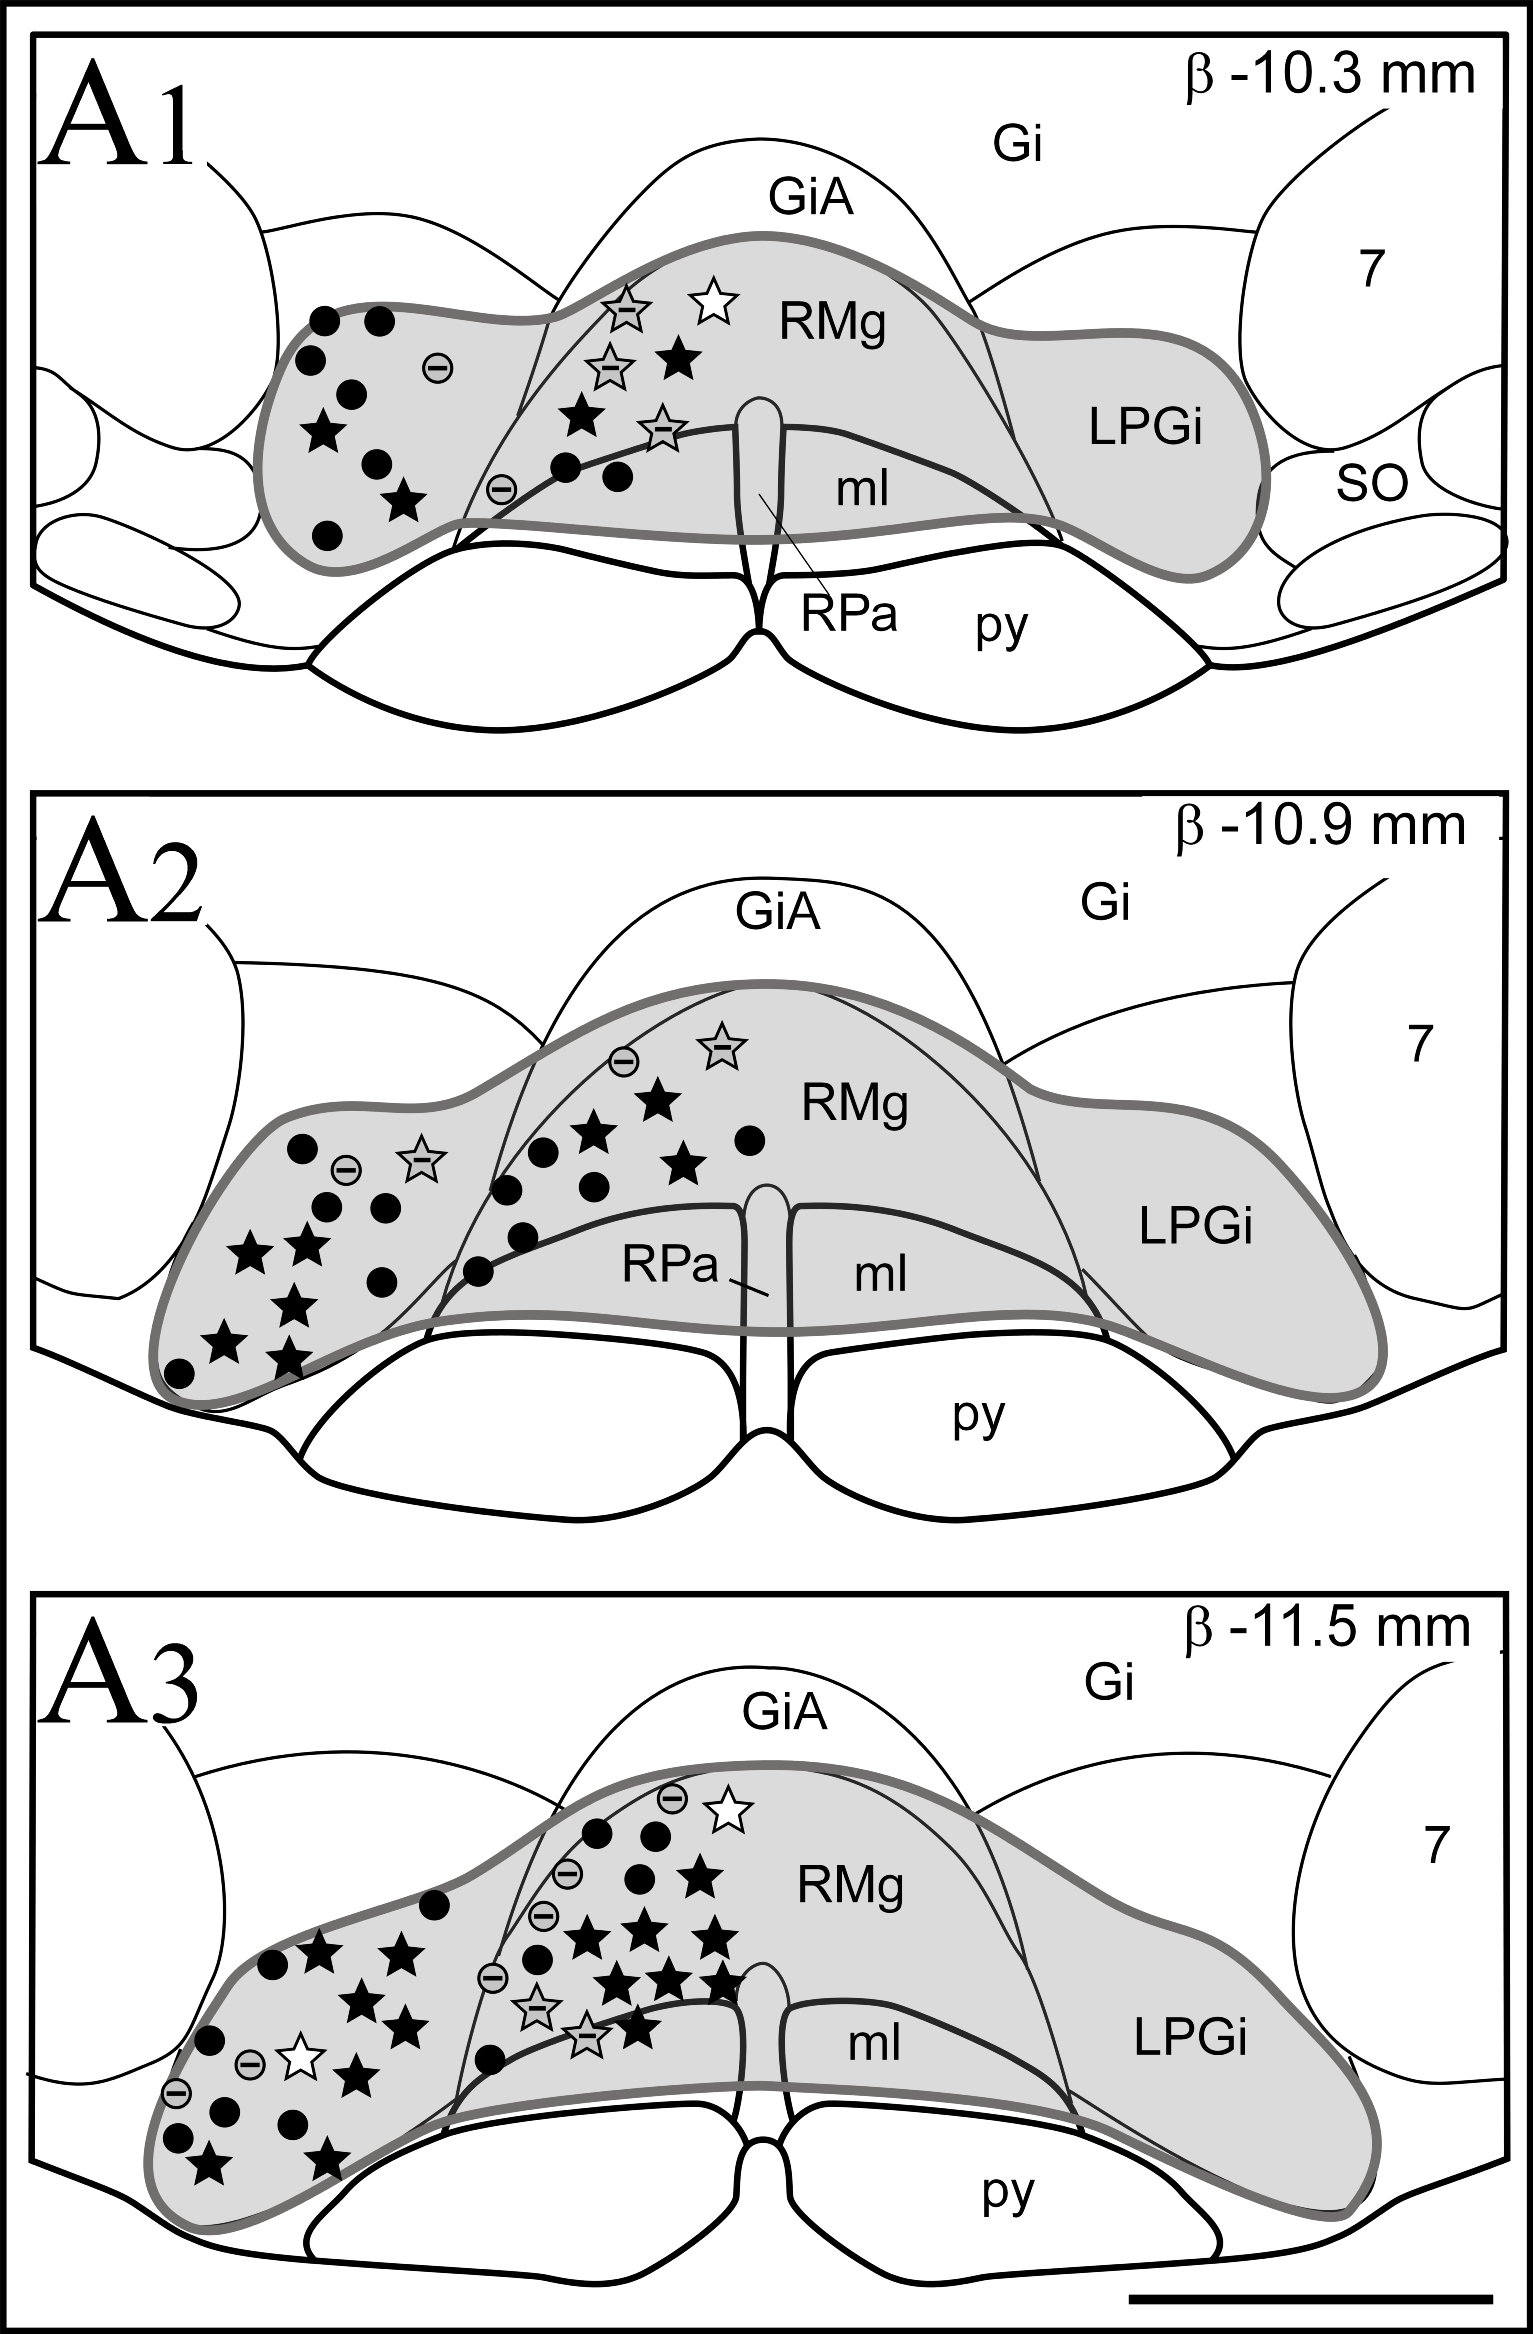
\includegraphics[scale=1]{Article3-FIG1.jpg} 
\end{center}

\caption[Location of recorded neurons in the B3 group]{\textbf{Location of neurons recorded and juxtacellularly injected in the B3 group including the LPGi and the RMg}}

{\protect\parbox[t]{18cm}{
\begin{small}
\textbf{(A1–A3)}: Coronal sections through the B3 group from rostral to caudal. Each level includes 600 µm rostrocaudal extent.\\
Star: serotonergic neurons. Circle: non-serotonergic neurons. Black filling: neuron activated by noxious stimuli. Grey filling + dash: neuron inhibited by noxious stimuli. White filling: unresponsive neurons. Grey area: region containing most serotonergic neurons. 7: nucleus of the 7th nerve; $\beta$: level caudal to Bregma in mm with minus sign (Paxinos and Watson, 2005); GiA: gigantocellular reticular nucleus: alpha part; Gi: gigantocellular reticular nucleus; LPGi: lateral paragigantocellular reticular nucleus; ml: medial lemniscus; py: pyramidal tract; RMg: raphe magnus nucleus; SO: superior olivary nucleus. Scale bar: 1 mm.
\end{small}}}

\label{Article3-FIG1}

\end{figure}

\subsubsection{LPGi serotonergic neurons}

LPGi serotonergic neurons had a slow (1.5 $\pm$ 0.2 Hz, 0.4-2.9 Hz range) and regular spontaneous discharge (CV$_{ISI}$ = 0.46 $\pm$ 0.04). Almost all LPGi serotonergic neurons (88\%, 14 in 16) responded markedly to strong noxious thermal stimulations and had a generally large receptive field with a moderate contralateral predominance. The response consisted in a tonic increase in discharge during the whole stimulation, followed by a short-lived post-discharge, with a mean response of 2.6 $\pm$ 0.3 Hz above the background discharge (1.1-5.4 Hz range, n = 14). Figure \ref{Article3-FIG2} A1 illustrates the clear increase of firing and a moderate spike depolarization of a well-isolated single-unit, during a 20 s dipping of the contralateral hind paw in 52 °C noxious water bath (Figure \ref{Article3-FIG2} B - page \pageref{Article3-FIG2}). These neurons responded similarly to noxious mechanical stimulation (pinch), but none responded to light mechanical or thermal stimulation. Figure \ref{Article3-FIG2} C illustrates the good encoding of increasing temperatures from 48 °C threshold, the mean population threshold being 48.3 $\pm$ 0.3 °C (n = 14). Only one LPGi serotonergic neuron was unresponsive (6\%, 1 in 16) and one was inhibited (6\%, 1 in 16) by noxious stimulation. Figure \ref{Article3-FIG2} D indicates the location of the typical neurons presented above within the LPGi serotonergic group, as well as its double labeling for both neurobiotin and 5-HT, analyzed in confocal microscopy.

\begin{figure}[p]

\begin{center}
 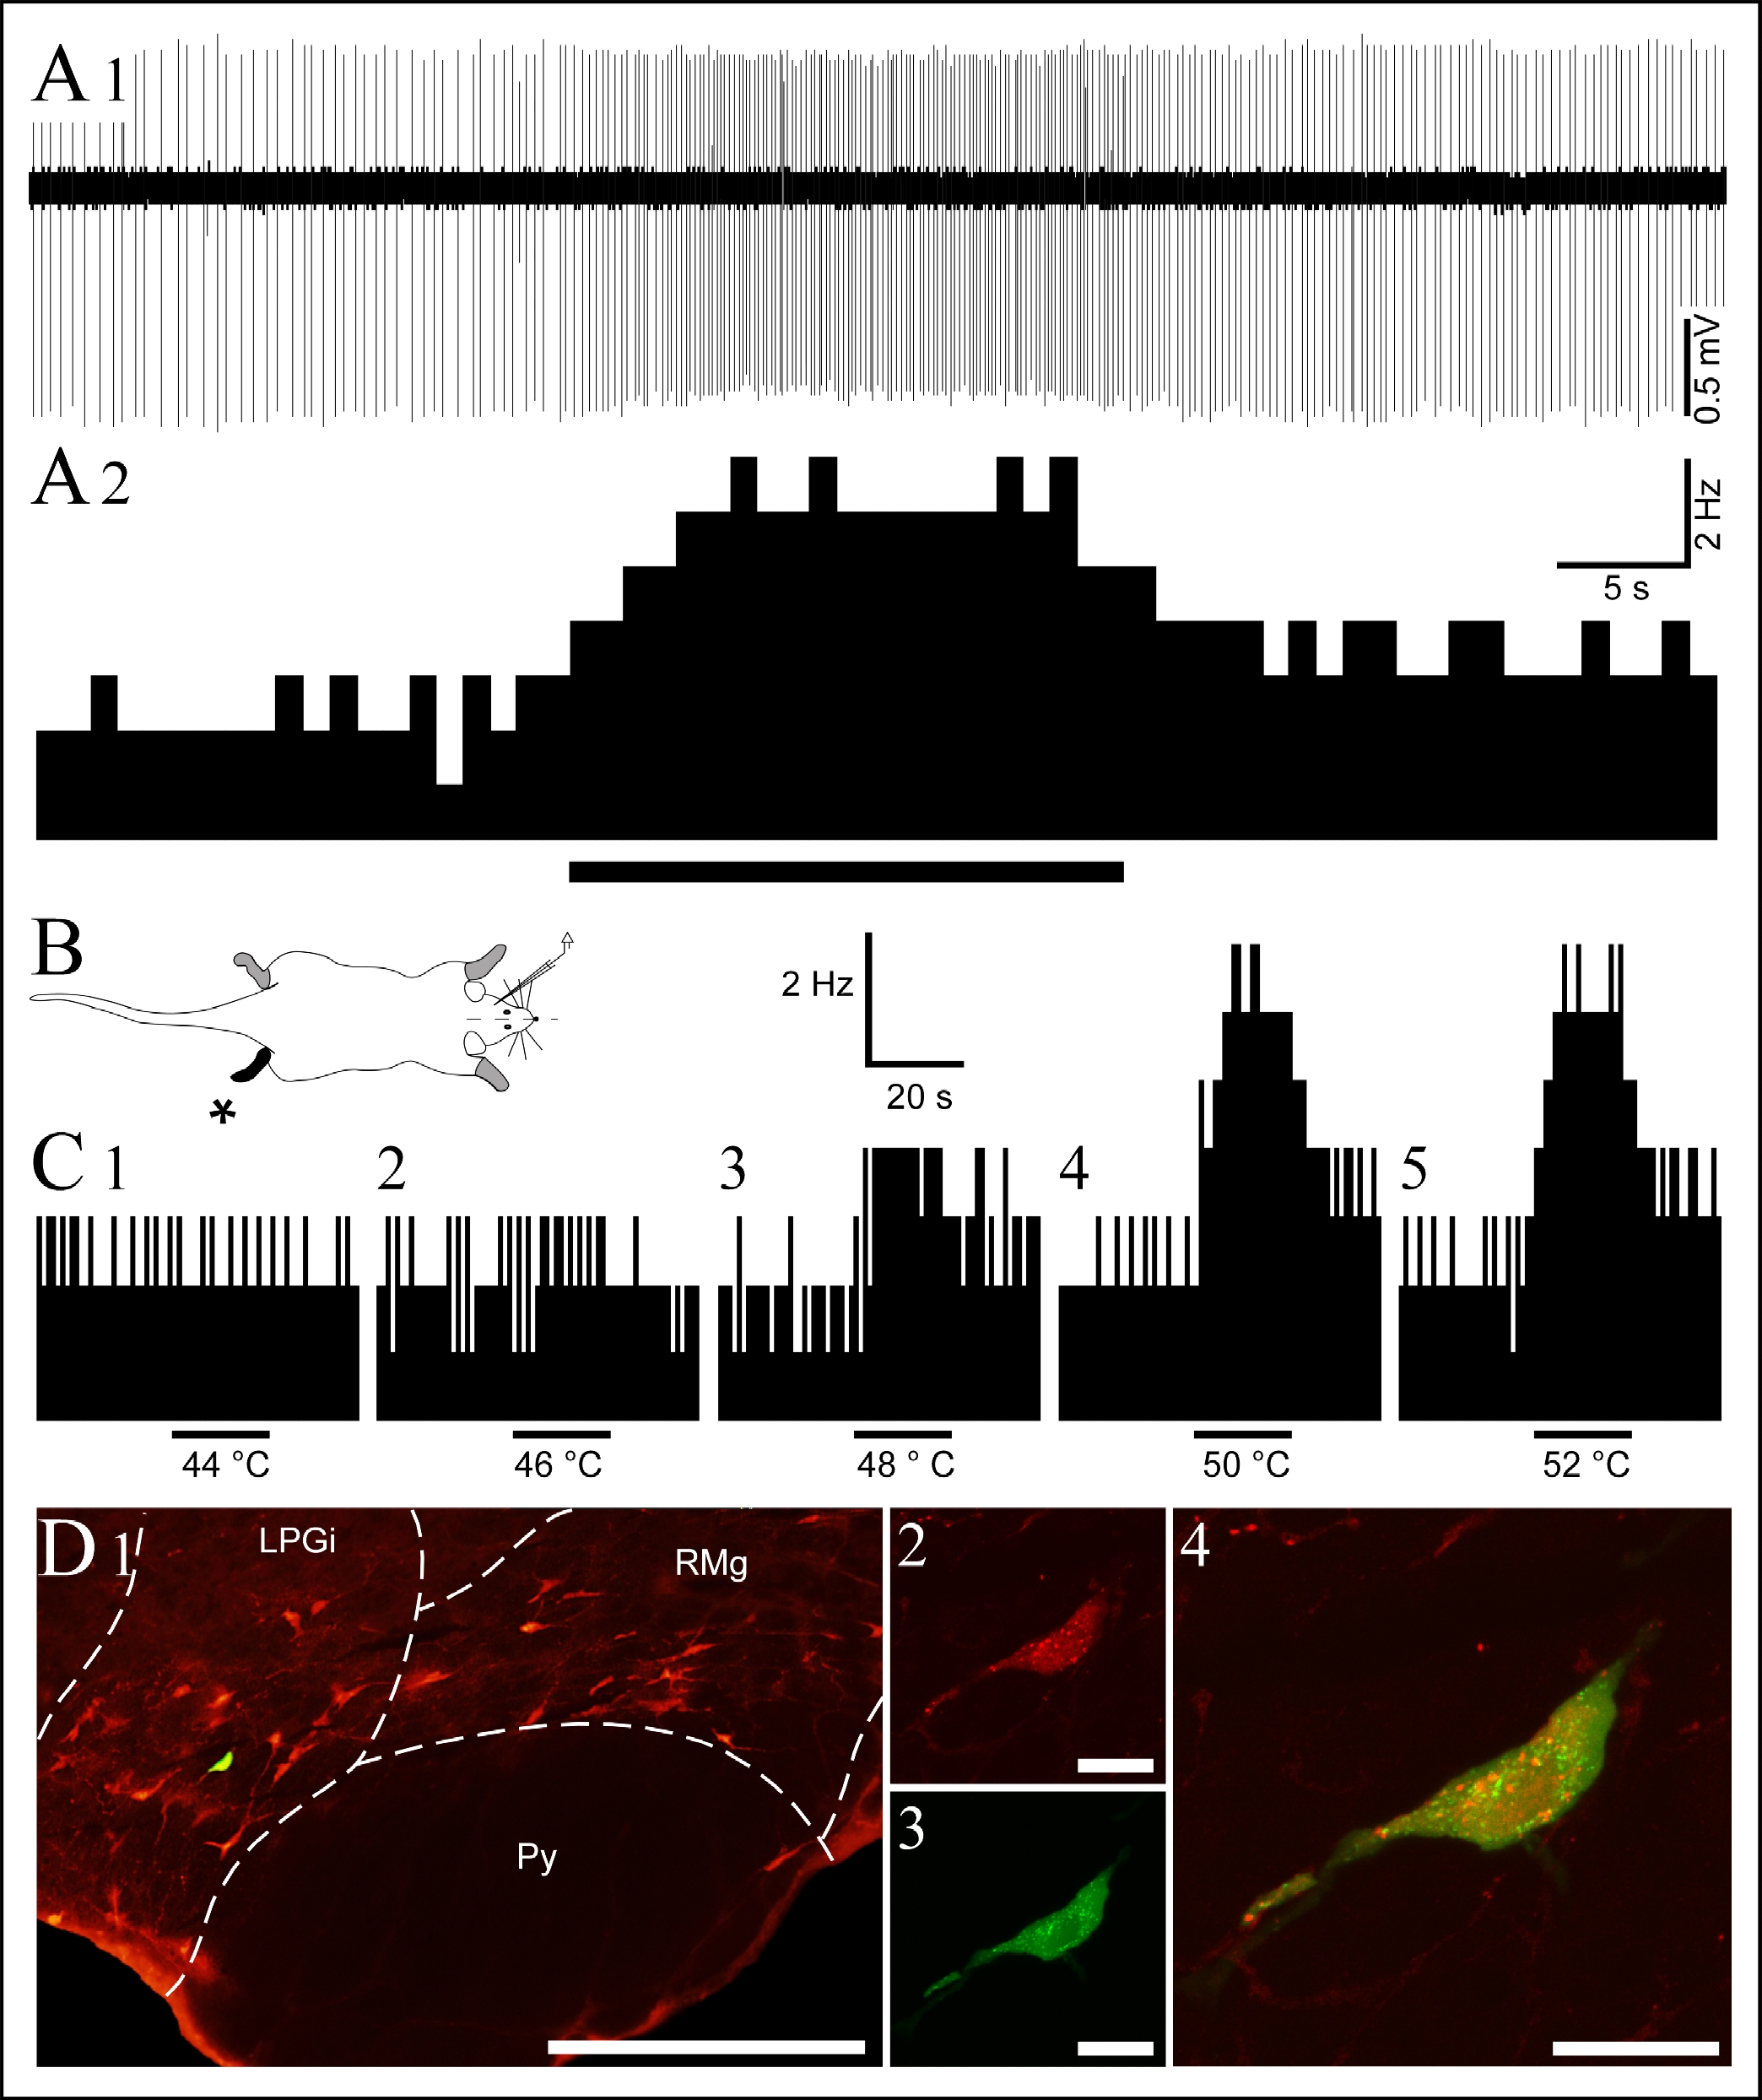
\includegraphics[scale=0.9]{Article3-FIG2.jpg} 
\end{center}

\caption[LPGi 5-HT neuron activated by noxious stimuli]{\textbf{Serotonergic neuron activated by noxious stimuli within the LPGi and juxtacellularly filled with neurobiotin}}

{\protect\parbox[t]{18cm}{
\begin{small}
\textbf{(A1-A2)}: Activation during 52 °C noxious stimulation (bar, 20 s duration) shown with both spikes (A1) and 2 s bin size histogram (A2).\\ 
\textbf{(B)}: Receptive field including higher (contralateral hind paw, black) and lower (other paws, gray) sensitivity cutaneous region.\\ 
\textbf{(C1-C5)}: Responses to graded thermal stimuli (bar: 20 s duration; 2 °C steps) from innocuous to strongly noxious temperature (44-52 °C), with 48 °C threshold.\\ 
\textbf{(D1)}: Low magnification epifluorescent microphotograph of the LPGi neuron double-labeled for neurobiotin and 5-HT (light green) within the serotonergic group of cells (red).\\ 
\textbf{(D2-D4)}: High magnification confocal images of the same neuron for 5-HT in red (D2), for neurobiotin in green (D3) and the superimposition of both labeling (D4).\\ 
LPGi, lateral paragigantocellular reticular nucleus; py, pyramidal tract; RMg, raphe Magnus nucleus. Scale bars: D1, 500 µm; D2-D4, 25 µm.
\end{small}}}

\label{Article3-FIG2}

\end{figure}

\subsubsection{Comparison of LPGi and RMg serotonergic neurons}

Serotonergic neurons of the RMg had a similarly slow (1.3 $\pm$ 0.1 Hz, 0.4-2.6 Hz range, n = 21) but slightly more regular (CV$_{ISI}$ = 0.37 $\pm$ 0.03, p < 0.05) spontaneous discharge than their LPGi counterparts (see above). A smaller proportion of RMg serotonergic neurons (61\%, 13 in 21) were excited by noxious thermal stimulations (mean response: 1.8 $\pm$ 0.4 Hz, 0.5-5.5 Hz range, n = 13). These neurons had large receptive fields, comparable to those of LPGi serotonergic neurons. Figure \ref{Article3-FIG3} A-C illustrates the often moderate increase of RMg serotonergic unit firing during 52 °C noxious stimulation, with moderate encoding properties (50°C threshold) and a large receptive field. The mean threshold of the RMg serotonergic population (48.6 $\pm$ 0.5°C, n = 13) was comparable to that of LPGi serotonergic neurons. In the RMg, a higher proportion of serotonergic neurons (29\%, 6 in 21), than in the LPGi, decreased their firing by 50 $\pm$ 8\% in response to noxious stimulation, or were unresponsive (10\%, 2 in 21). The serotonergic phenotype of all RMg serotonergic neurons was also unambiguously determined with epifluorescent illumination and confocal microscopy (Figure \ref{Article3-FIG3} D - page \pageref{Article3-FIG3}).

To assess at the best the difference between LPGi and RMg serotonergic populations, we built mean population responses of all LPGi (Figure \ref{Article3-FIG4} A1 - page \pageref{Article3-FIG4}, n = 16) and all RMg (Figure \ref{Article3-FIG4} A2 - page \pageref{Article3-FIG4}, n = 21) serotonergic neurons. This population analysis revealed indisputably the marked intensity as well as the coherence and tonicity of the LPGi population response to noxious heat (Figure \ref{Article3-FIG4} A1 - page \pageref{Article3-FIG4}), whereas the response of its RMg counterpart appears clearly weaker (Figure \ref{Article3-FIG4} A2 - page \pageref{Article3-FIG4}). Thus, the mean LPGi population response (2.2 $\pm$ 0.4 Hz above spontaneous activity, n = 16) is significantly higher (p < 0.01) than its RMg counterpart (1.0 $\pm$ 0.3 Hz, n = 21). The difference between these populations resulted from two combined factors: 1) a higher proportion of activated units in LPGi group (Figure \ref{Article3-FIG4} B - page \pageref{Article3-FIG4}) and 2) a higher excitation magnitude of neurons activated (Figure \ref{Article3-FIG4} C - page \pageref{Article3-FIG4}). Interestingly, Figure 4 C shows the good encoding properties of LPGi activated serotonergic neurons with high slope steepest point (49.3 $\pm$ 0.3 °C, n = 9) comparable to the one of RMg activated serotonergic neurons (49.8 $\pm$ 0.5 °C, n = 13).

\begin{figure}[p]

\begin{center}
 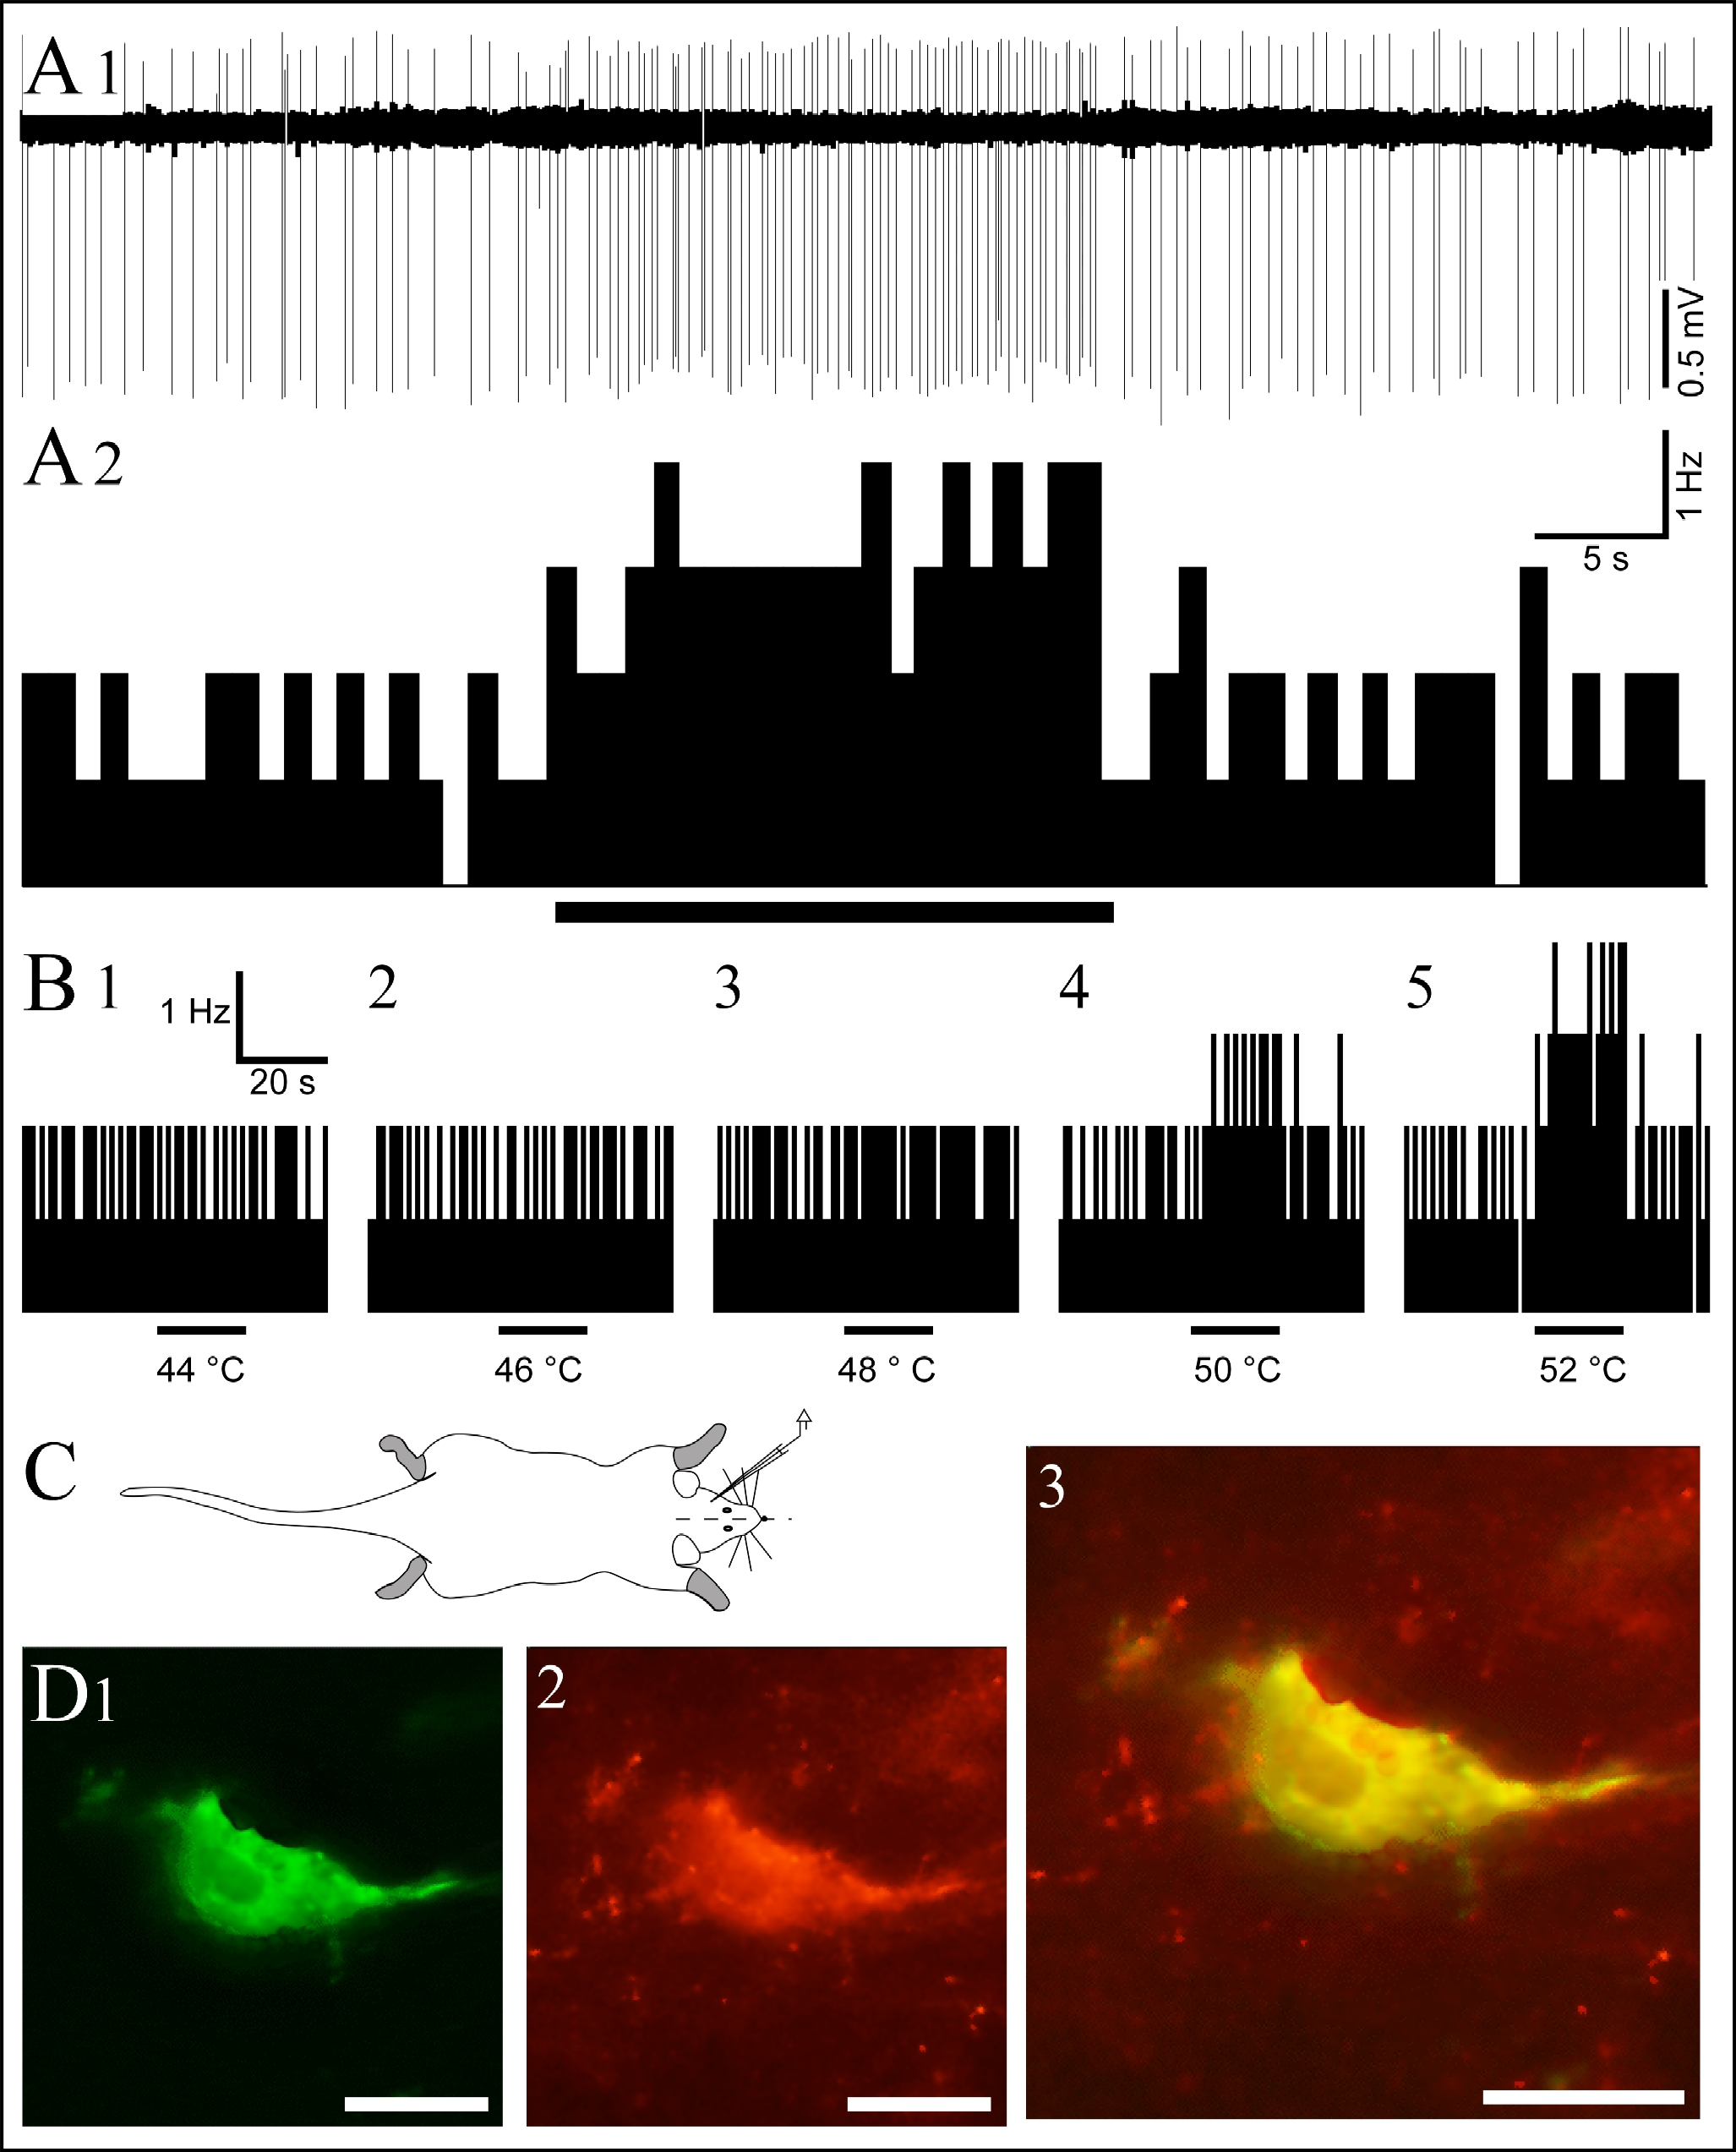
\includegraphics[scale=0.9]{Article3-FIG3.jpg} 
\end{center}

\caption[RMg 5-HT neuron activated by noxious stimuli]{\textbf{Serotonergic neuron activated by noxious stimuli within the RMg and juxtacellularly filled with neurobiotin}}

{\protect\parbox[t]{18cm}{
\begin{small}
\textbf{(A1-A2)}: Activation during 52 °C noxious stimulation (bar: 20 s duration) shown with both spikes (A1) and 2 s bin size histogram (A2).\\
\textbf{(B1-B5)}: Responses to graded thermal stimuli (bar: 20 s duration; 2 °C steps) from innocuous to strongly noxious temperature (44-52 °C), with 50 °C threshold.\\
\textbf{(C)}: Large receptive field including the four paws (gray).\\ 
\textbf{(D1-D3)}: Epifluorescent microphotographs of the RMg neuron double-labeled for neurobiotin in green (D1), 5-HT in red (D2). The superimposition of both labeling giving a yellow color (D3). \\
Scale bars: 25 µm.
\end{small}}}

\label{Article3-FIG3}

\end{figure}


\begin{figure}[p]

\begin{center}
 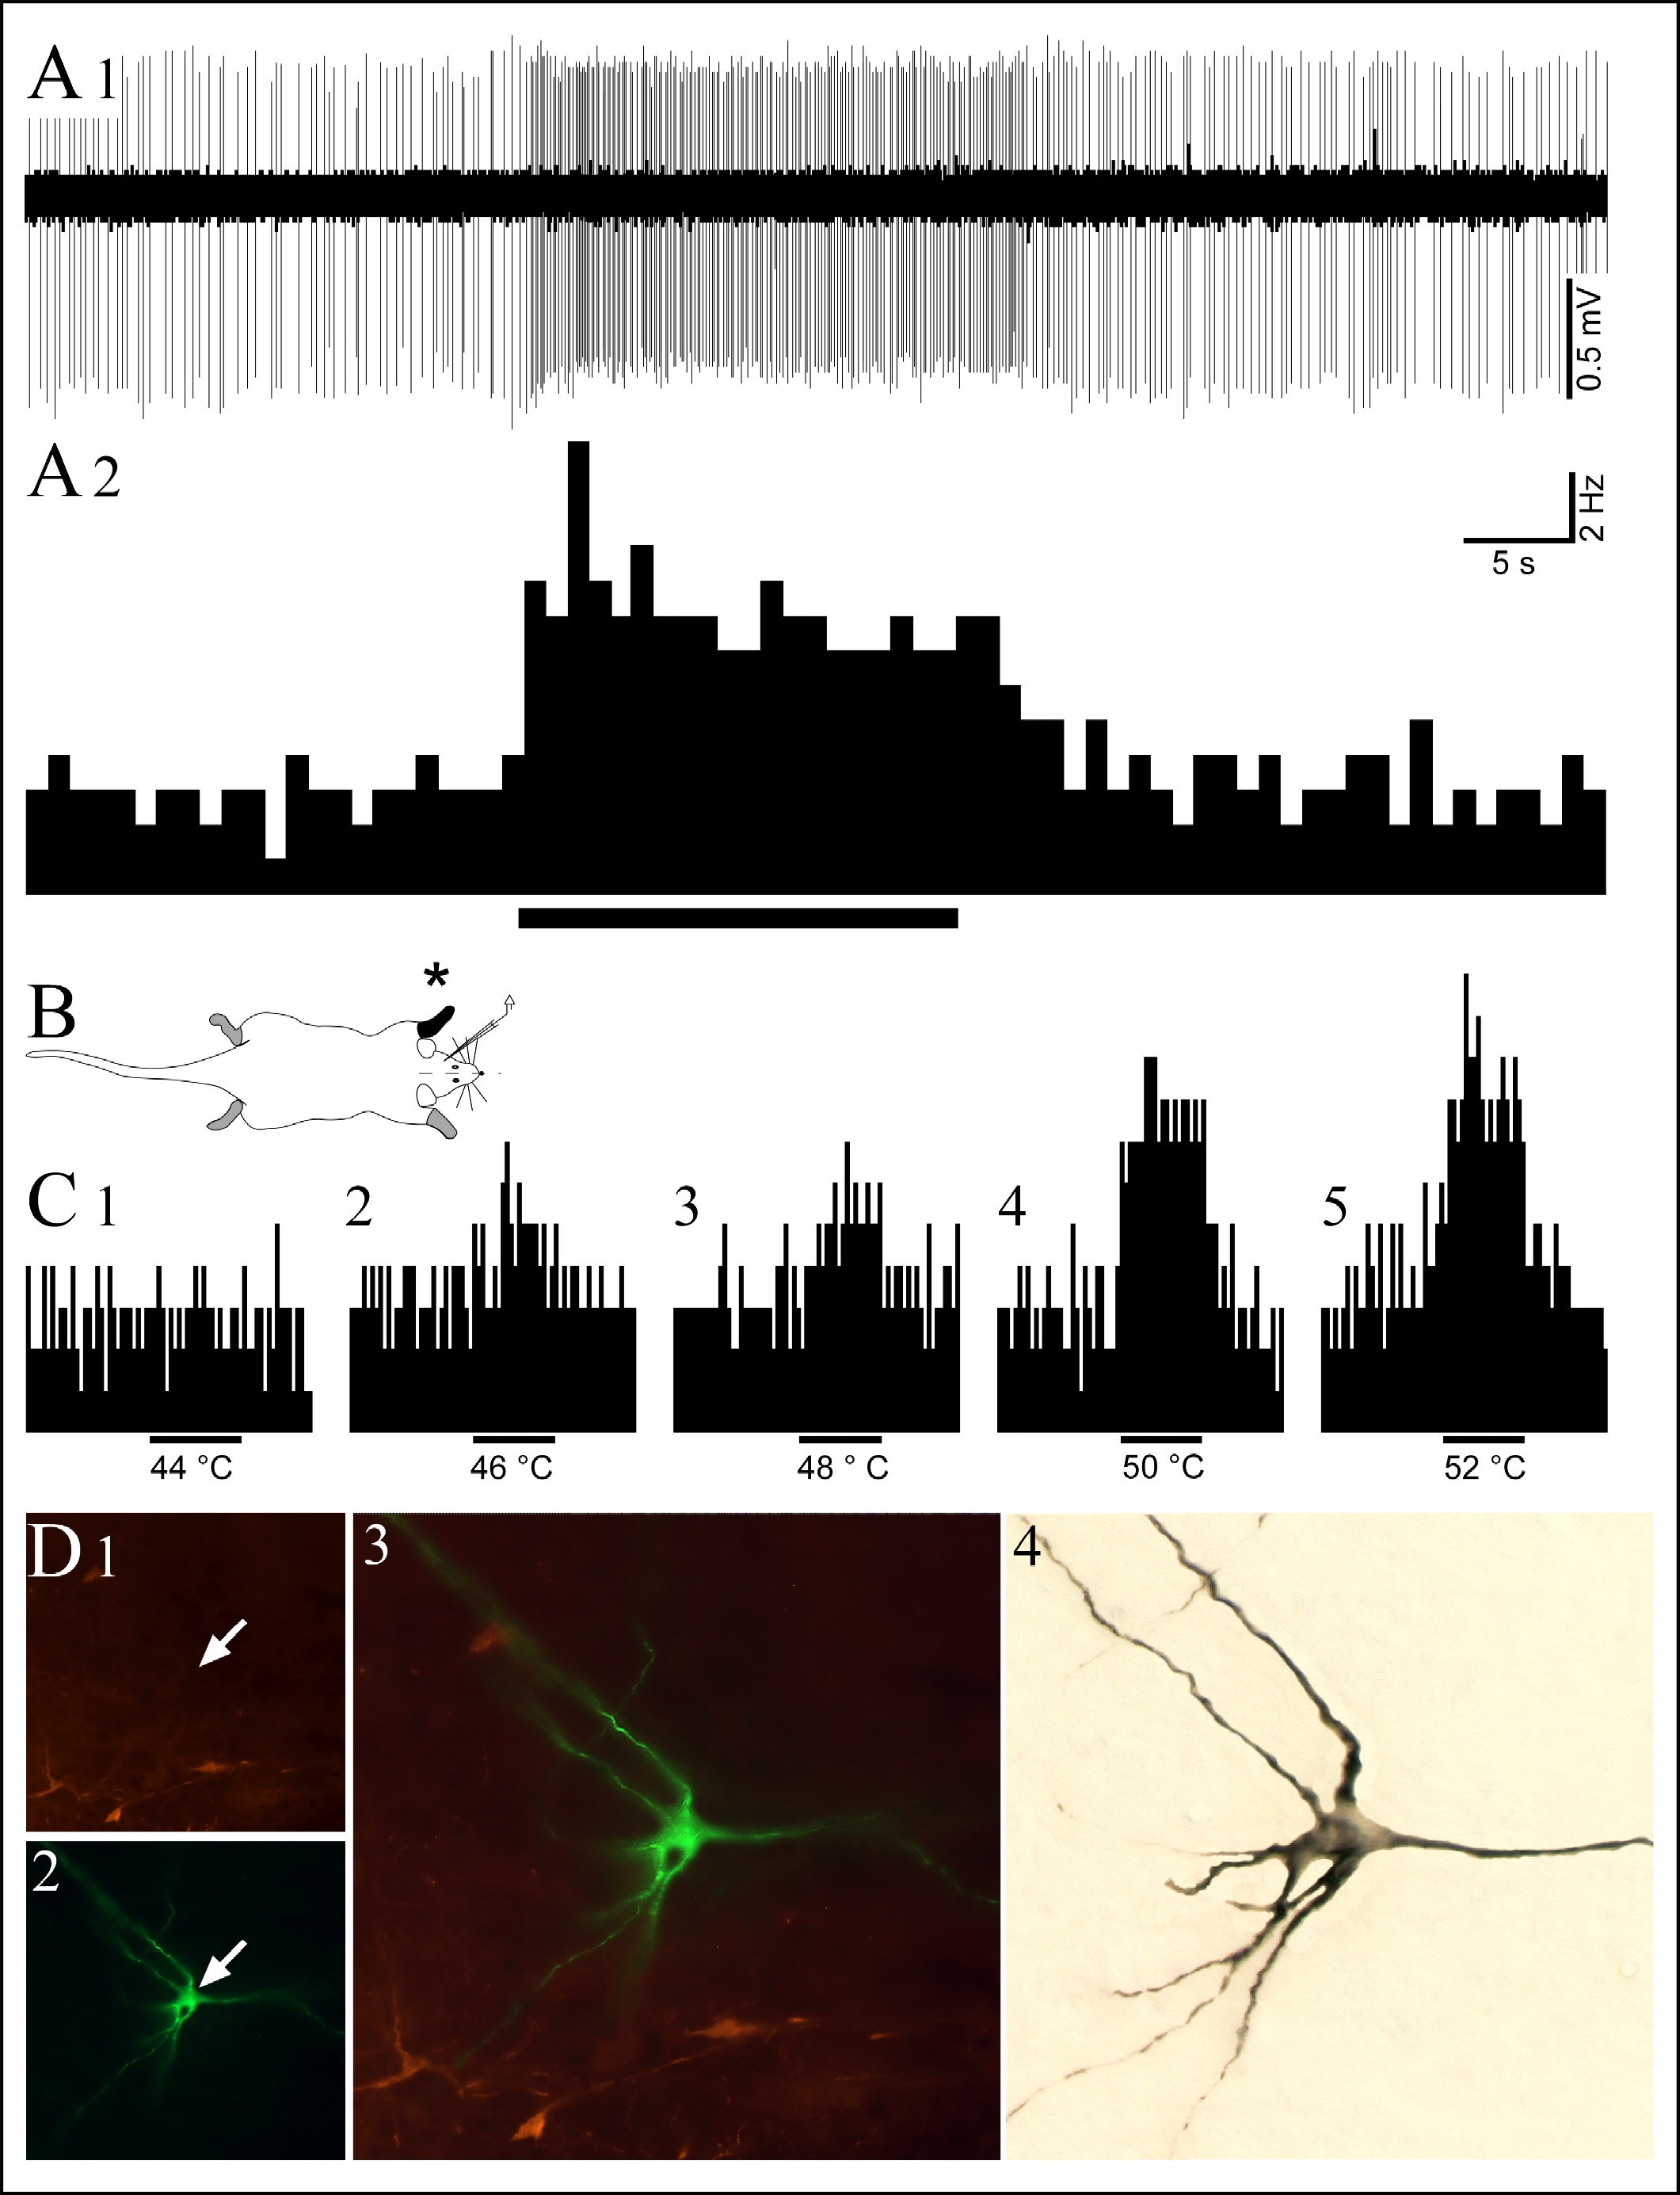
\includegraphics[scale=0.85]{Article3-FIG4.jpg} 
\end{center}

\caption{\textbf{Comparison of RMg and LPGi serotonergic neurons}}

{\protect\parbox[t]{18cm}{
\begin{small}
\textbf{(A)}: Mean population response to thermal noxious stimuli of serotonergic neurons recorded in the LPGi (A1 – n = 16) and the RMg (A2 - n = 21), shown with 2 s bin size histogram (black; vertical bar: SEM) aligned to the 20 s duration stimulus onset (thick bar).\\
\textbf{(B)}: Response class histogram of serotonergic neurons in LPGi (black, n = 16) and RMg (gray, n = 21). 
Abscissa: inhibited, unresponsive, and activated (0.3 to 6 Hz) neurons; ordinate: percentage of neurons in each class for LPGi and RMg neurons.\\
\textbf{(C)}: Mean stimulus–response curves (vertical bar: SEM) to graded thermal stimuli for activated serotonergic neurons in the LPGi (solid line, n = 9) and the RMg (dashed line, n = 13).\\
Abscissa: stimulus temperature; ordinate: mean response frequency.
\end{small}}}

\label{Article3-FIG4}

\end{figure}

\subsubsection{Comparisons of serotonergic with non-serotonergic neurons}

For simplicity we pooled on one-side LPGi and RMg serotonergic neurons (n = 37) and on other-side LPGi and RMg non-serotonergic neurons (n = 40). Note that more individualized comparisons did not bring much more information than comparisons in previous section.

The spontaneous discharge of non-serotonergic neurons was significantly higher (6.3 $\pm$ 1.2 Hz, n = 40) and more irregular (CV$_{ISI}$ = 0.79 $\pm$ 0.08), compared to the slow frequency (1.4 $\pm$ 0.1 Hz, n = 37) and regular (CV$_{ISI}$ = 0.41 $\pm$ 0.02) discharge of serotonergic neurons (p < 0.001 in both cases). The proportions of non-serotonergic neurons activated (75\%, 30 in 40), unresponsive (0\%, 0 in 40) or inhibited (25\%, 10 in 40) by noxious thermal stimuli were similar to those of serotonergic neurons (73, 8, 19\%, respectively, n = 37). Figure \ref{Article3-FIG5} A illustrates the often marked increase of a non-serotonergic unit firing during 50 °C noxious stimulation with a sharp onset, a sustained but decreasing discharge and a clear offset. \ref{Article3-FIG5} B-C illustrates the progressive increasing of response from 46 °C (the threshold) up to 52 °C (Figure \ref{Article3-FIG5} C - page \pageref{Article3-FIG5}), indicating good encoding properties. The mean threshold of non-serotonergic neurons was high (47.6 $\pm$ 0.4 °C, n = 40) but still lower than the one of serotonergic neurons (48.6 $\pm$ 0.3 °C, n = 34, p < 0.05). Importantly, each of the non-serotonergic neurons was identified by the absence of 5-HT labeling superimposed to the soma labeled by neurobiotin (Figure \ref{Article3-FIG4} D - page \pageref{Article3-FIG4}). 

The response of non-serotonergic neurons activated by noxious stimulation (8.0 $\pm$ 1.2 Hz, n = 30) was significantly higher (p < 0.001) than that of activated serotonergic neurons (2.2 $\pm$ 0.3 Hz, n = 27). This marked difference is illustrated in Figure \ref{Article3-FIG6} A that compared the mean population response of 27 serotonergic neurons (black) with the one of 30 non-serotonergic neurons (grey). It can also be observed that the response onset of non-serotonergic neurons was sharper whereas the response of serotonergic neurons was more sustained. Importantly, not any neurons of both population responded to stimulus < 44 °C. Both populations clearly encoded thermal noxious stimuli with a higher activation of non-serotonergic neurons for every temperature tested (Figure \ref{Article3-FIG6} B - page \pageref{Article3-FIG6}). The steepest portion of response curves was very high for both population but with a tendency (p < 0.1) to be higher for serotonergic neurons (49.6° $\pm$ 0.2 °C, n = 22) than for non-serotonergic neurons (49.0° $\pm$ 0.3 °C, n = 17).
In the population of inhibited neurons, the relative discharge decrease was more pronounced (p < 0.01) for non-serotonergic (77 $\pm$ 5\%, n = 10) than for serotonergic neurons (51 $\pm$ 7\%, n = 7).

\begin{figure}[p]

\begin{center}
 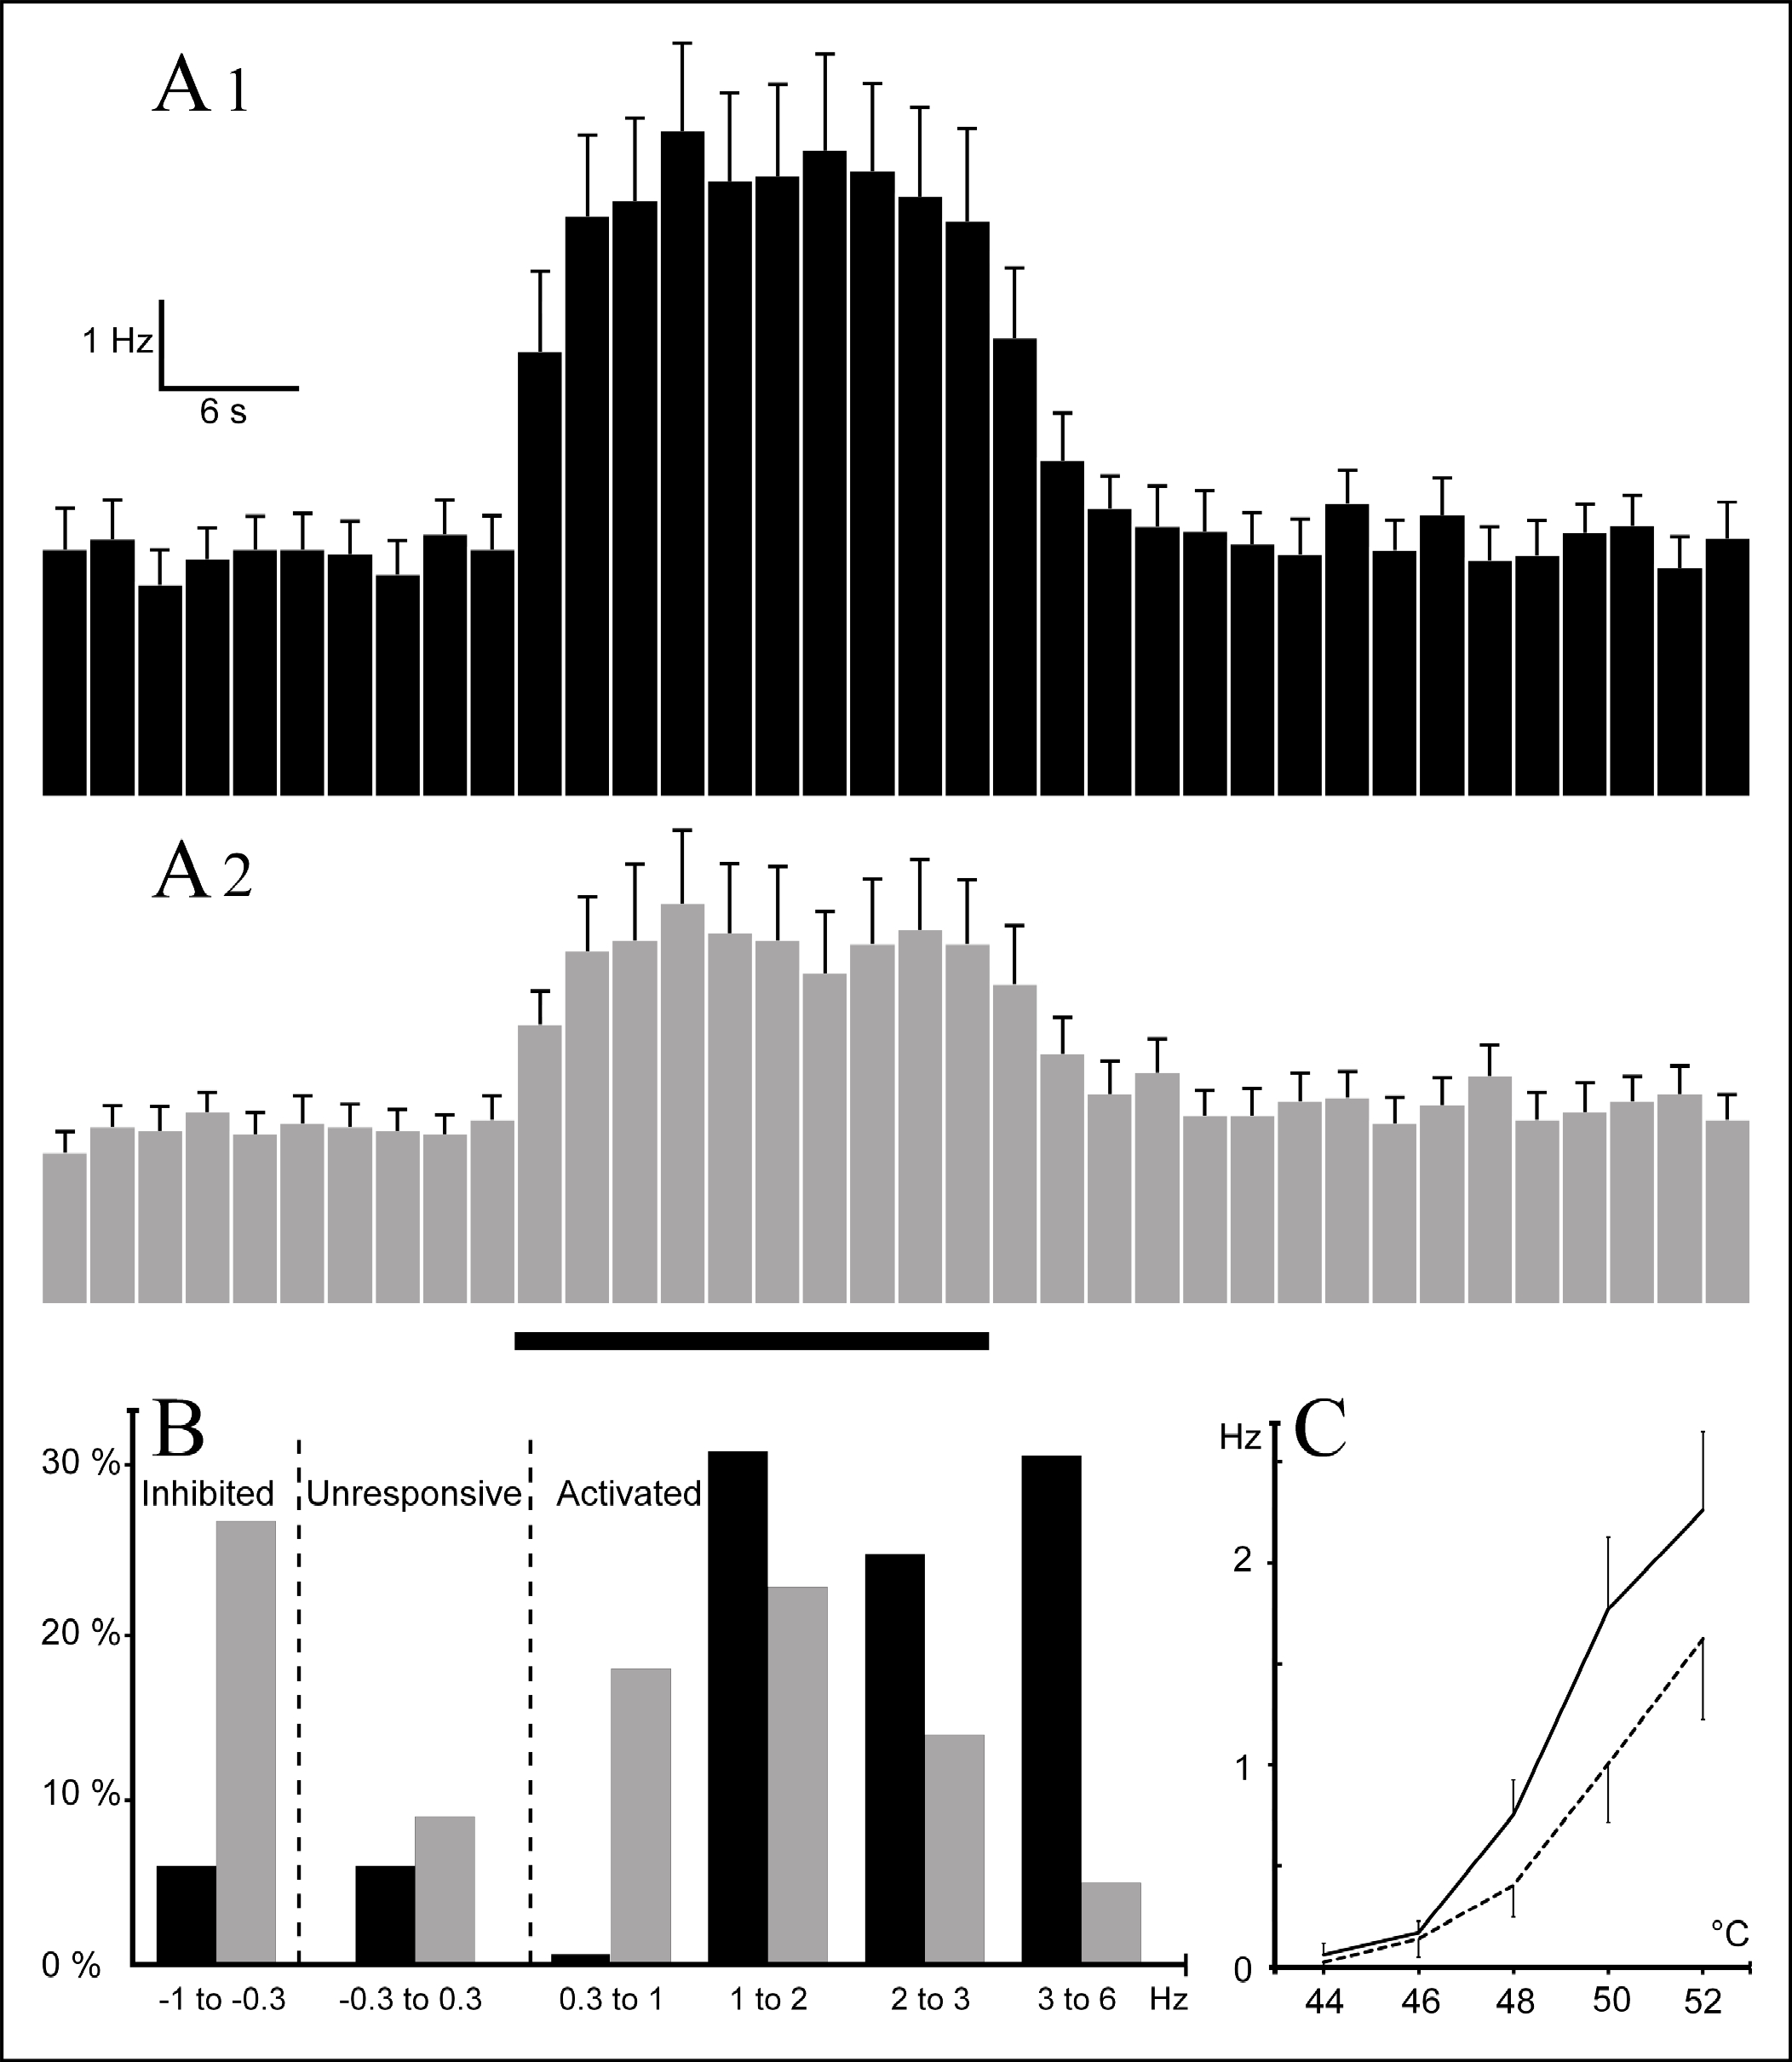
\includegraphics[scale=0.9]{Article3-FIG5.jpg} 
\end{center}

\caption[LPGi non-5-HT neuron activated by noxious stimuli]{\textbf{Non-serotonergic neuron activated by noxious stimuli within the LPGi and juxtacellularly filled with neurobiotin}}

{\protect\parbox[t]{18cm}{
\begin{small}
\textbf{(A1-A2):} Activation during 50 °C noxious stimulation (bar: 20 s duration) shown with both spikes (A1) and 2 s bin size histogram (A2).\\
\textbf{(B)}: Receptive field including higher (ipsilateral forepaw, black) and lower (other paws, gray) sensitivity cutaneous region.\\
\textbf{(C1-C5)} Response to graded thermal stimuli (bar: 20 s duration; 2 °C steps) from innocuous to strongly noxious temperature (44-52 °C), with 46 °C threshold.\\
\textbf{(D1-D3)}: Epifluorescent microphotographs of the LPGi neuron single-labeled for neurobiotin in green (D2, arrow), without labeling for 5-HT (D1, arrow). The superimposition of both plan exhibited only the neurobiotin green color (D3). D4, Microphotograph of the same neuron after labeling of the neurobiotin with DAB/Ni reaction (see Methods).\\ 
Scale bars: 25 µm.
\end{small}}}

\label{Article3-FIG5}

\end{figure}

\subsubsection{Electrophysiological differentiation of serotonergic with non-serotonergic neurons }

The waveforms of serotonergic and non-serotonergic spikes were markedly different (Figure \ref{Article3-FIG6} C - page \pageref{Article3-FIG6}): 1) the duration of serotonergic spikes (3.6 $\pm$ 0.2 ms, n = 37) was significantly longer (p < 0.001) than the one of non-serotonergic spike (2.1 $\pm$ 0.1 ms, n = 40).
Each of the recorded neurons was classified according 1) to its mean ISI ($\bar{X}$, in ms) and 2) the SD of the ISI (s in ms) with regard to a straight line representing the discriminant function $146-\bar{X}+0.98s=0$ (see Methods). From Mason (1997), neurons above the line should be non-serotonergic and neurons below the line should be serotonergic (Figure \ref{Article3-FIG6} D - page \pageref{Article3-FIG6}). In the present experiment all the serotonergic identified neurons were adequately located below the line, but only a majority of non-serotonergic identified neurons (63\%, 25 in 40) were adequately located above the line. Thus, surprisingly, one third of non-serotonergic identified neurons (37\%, 15 in 40) were located below the line, mixed with serotonergic neurons (Figure \ref{Article3-FIG6} D - page \pageref{Article3-FIG6}). Thus, in the case of the present data the discriminant function was able to classify adequately as non-serotonergic all the neurons above the curve and as serotonergic 72\% (37 in 52) of the neurons below the line but would have miss-attributed the serotonergic status to 28\% (15 in 52) of neurons below the curve.

\begin{figure}[p]

\begin{center}
 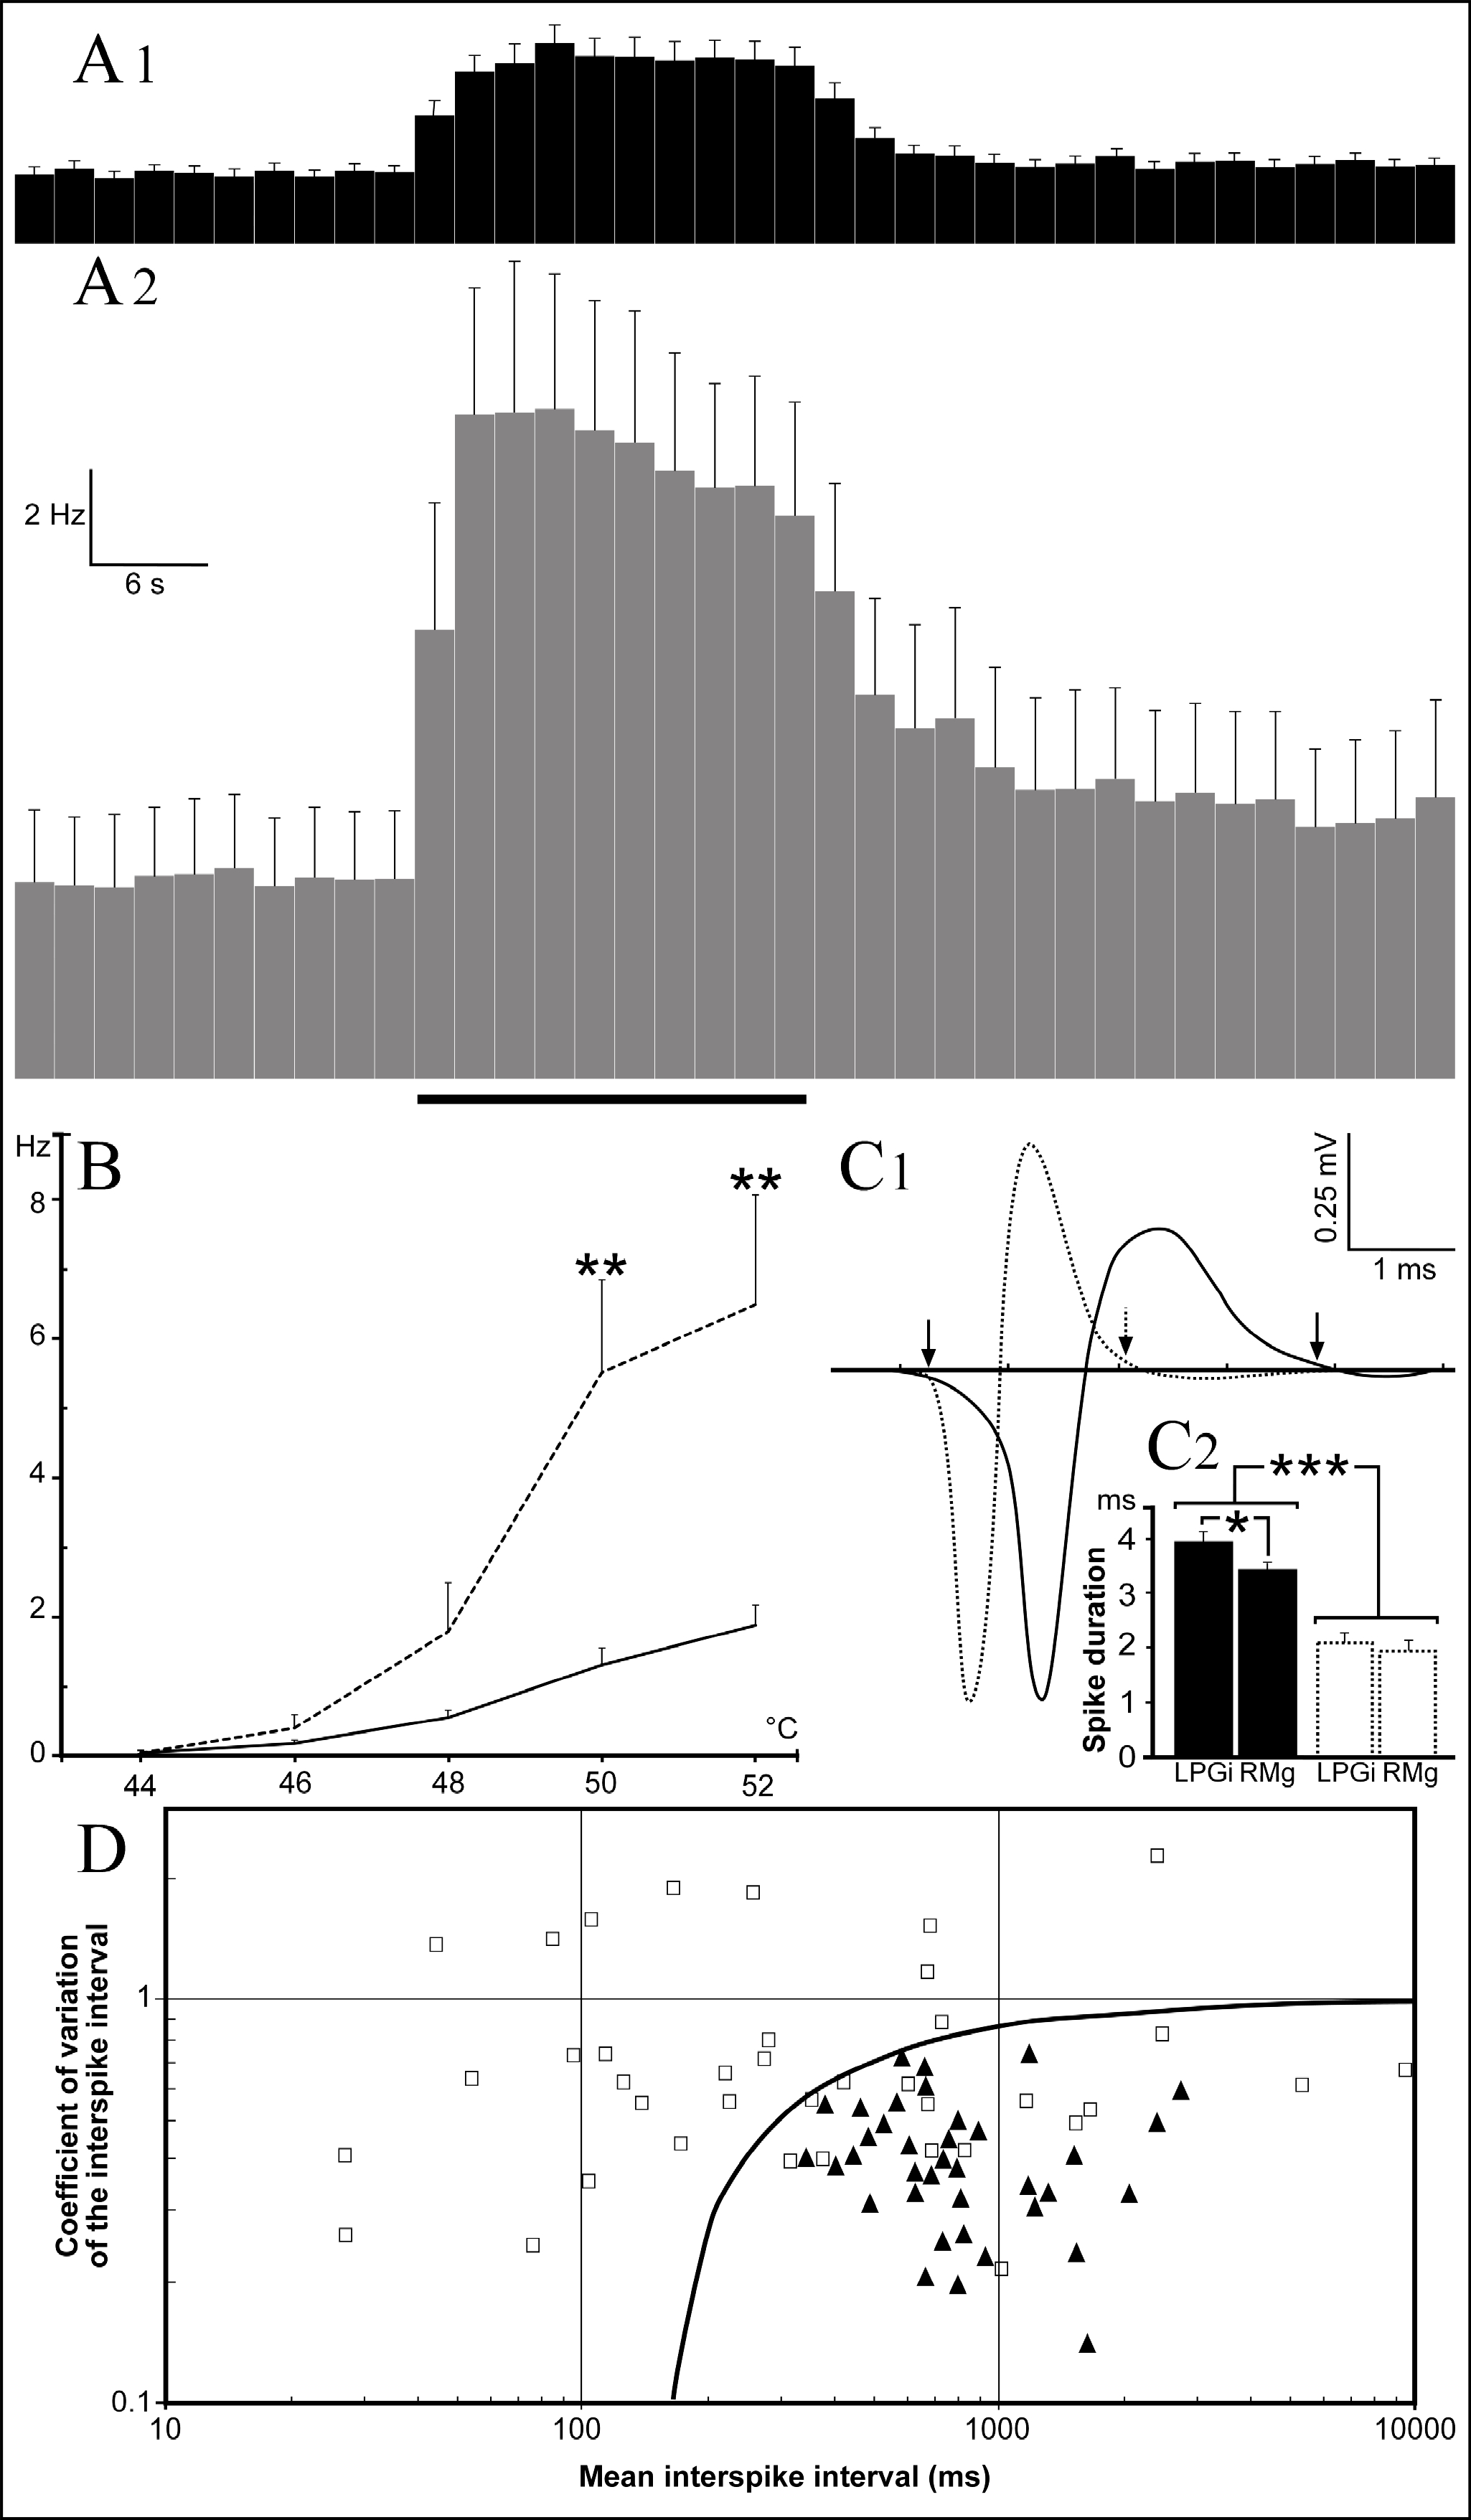
\includegraphics[scale=0.65]{Article3-FIG6.jpg} 
\end{center}
\caption{\textbf{Comparison of serotonergic and non-serotonergic neurons}}

{\protect\parbox[t]{18cm}{
\begin{scriptsize}
\textbf{(A)}: Mean population response of serotonergic (A1, black, n = 27) and non-serotonergic (A2, gray, n = 30) neurons activated by thermal noxious stimuli, shown with histogram (vertical bar: SEM) aligned to the 20 s duration stimulus onset (thick bar).\\ 
\textbf{(B)}: Mean stimulus–response curves (vertical bar: SEM) of activated serotonergic (solid line, n = 22) and non-serotonergic (dashed line, n = 17) neurons. Abscissa: stimulus temperature; ordinate: mean response frequency.\\ 
\textbf{(C1)}: Differences between serotonergic (solid line) and non-serotonergic (dotted line) averaged spike waveforms. The non serotonergic waveform was normalized to have the same minimum value as that of the serotonergic. Arrows: measurement points.\\ 
\textbf{(C2)}: Mean (+ SEM) spike duration of LPGi and RMg serotonergic (black, n = 16 and 21) and non-serotonergic (dotted lines, n = 21 and 19), respectively. $*$: p < 0.05; $**$: p < 0.01; $***$: p < 0.001.\\ 
\textbf{(D)}: Characteristics of spontaneous discharge of serotonergic (black triangles) and non-serotonergic (white squares) cells. 
Abscissa: ISI; ordinate: CV of the ISI. The solid line represents the discriminant function $y(\bar{X},CV)=\frac{146}{\bar{X}}-1+0.98\times CV=0$ (Mason, 1997; see Methods) which defines the optimal boundary between serotonergic and non-serotonergic cells. Two neurons had so low a spontaneous discharge that they do not appear in this graph.
\end{scriptsize}}}

\label{Article3-FIG6}

\end{figure}

\subsection{DISCUSSION}

This study showed for the first time that almost all the serotonergic neurons (88\% from n = 16) located within the LPGi were clearly and tonically activated (2.6 $\pm$ 0.3 Hz above the background discharge) by strong thermal noxious stimuli. They also had a high threshold (48.3 $\pm$ 0.3°C) and a large receptive field.
For comparison purpose, serotonergic neurons were also recorded in the RMg. Surprisingly the responsiveness of these neurons was higher than expected. Nevertheless, the proportion of RMg activated neurons (61\%, n = 21) as well as the magnitude of their responses (1.8 $\pm$ 0.4 Hz), were lower than those found in the LPGi. The non-serotonergic neurons recorded within the boundaries of B3 group were often excited by noxious stimuli (75\% from n = 40) with, as expected, a higher magnitude of response (7.9 $\pm$ 1.2 Hz, n = 30) than the serotonergic ones.

\subsubsection{Comparison to previous c-fos studies}

To our knowledge, no electrophysiological study has systematically examined the response of LPGi serotonergic neurons to noxious stimuli. More indirect comparison indicates that, our finding that LPGi neurons were activated by strong noxious stimuli is in general agreement with previous c-fos and 2-deoxyglucose (Porro et al. 1991; Mao et al. 1993; Lanteri-Minet et al. 1994; Wang et al. 1995; Oh et al. 2006; Gau et al. 2009). In particular, our study is in good agreement with Gau et al. (2009) that showed that thermal noxious stimuli $\ge$ 48°C induced a marked increase of c-fos expression within the serotonergic neurons of the LPGi. However, the present study indicates that 88\% of LPGi serotonergic neurons were activated by 52 °C noxious stimuli, whereas a reasonable estimate from Gau et al. (2009) would indicate that the same stimuli increased c-fos expression in about 40\% of LPGi serotonergic neurons. This discrepancy may be due in part to the extent of the receptive field investigated (one region only in c-fos experiment, several regions in electrophysiology) but, most of this difference is certainly explained by a lower c-fos sensitivity compare to that of the electrophysiological technique (Bullitt 1989; Dragunow \& Faull 1989; Harris 1998).

\subsubsection{Comparison to previous electrophysiological studies}

Previous studies in anesthetized rats and using indirect means of identifying serotonergic neurons of the RMg gave conflicting results. Chiang and Gao showed that two thirds of those neurons were activated by noxious tail heat while the rest was inhibited (Chiang \& Gao 1986). Wessendorf et al showed that a majority of RMg serotonergic neurons are activated by noxious pinch but that most of them are unaffected by noxious heat (Wessendorf \& Anderson 1983). However these studies could only assume the serotonergic character of the recorded neurons. More recent studies, using direct immunohistological and/or a well validated algorithmic method of serotonergic neurons identification, consistently showed that most of these are unresponsive to noxious stimulations (Potrebic et al. 1994; Gao \& Mason 2000; Winkler et al. 2006) while a small percentage is slightly activated by noxious tail heat (Gao \& Mason 2000). Besides, one fifth of the serotonergic neurons of the RMg were slightly activated by noxious pinch but not noxious heat (Mason 1997), in accord with indirect evidence that these neurons might be preferentially activated by noxious mechanical stimuli (Karlsson et al. 2006; Bee \& Dickenson 2008).

Similarly to those studies, we found that the magnitude of the responses of serotonergic neurons activated by noxious, although stronger in our study, is rather limited. Most neurons did not increase their discharge by more than 150\% in response to these stimuli. This is in accord with in vitro electrophysiological studies showing that the maximum discharge these neurons is limited by their intrinsic membrane properties and that they very rarely fire at more than 8 Hz even when very strong depolarizing currents are injected (Bayliss et al. 1997b; 1997a; Li \& Bayliss 1998). Similarly, we found, in agreement with previous reports, that the responses of serotonergic neurons are limited to the time of the stimulation and do not show long lasting post discharges.

However, and in contrast to previous studies, we found a higher percentage of activated neurons (61\% in our study compared to 17\% in Gao \& Mason [2000]) with higher response intensities and equal sensitivity to thermal and mechanical stimuli. It is unlikely that this difference arose from different data analysis as we used a method very similar to the one used in the previous works. However, several reasons might explain part of these differences. Firstly, we used a longer stimulation time (20 s), whereas many previous studies used short stimuli ($\approx$ 6 s) (Mason 1997; Gao \& Mason 2000). Retrospectively, it is likely that applying 52°C noxious stimuli during 6 s would have decreased the proportion of neurons recognized as activated: all the low responding neurons would have been classified as unresponsive. Secondly, in previous studies, noxious heat stimuli were mostly applied to the tail whereas we tested several body parts. Even though most cells of the rostroventromedial medulla (RVM) have large receptive field, it might be inappropriate to generalize the response of a cell by testing only a part of this field. Such conclusions have been drawn by others concerning the non serotonergic cells of this region (Ellrich et al. 2001b; Schnell et al. 2002). Our results suggest that this might also be true for the serotonergic neurons of the RVM. 

However, most of the discrepancy is likely due to the difference in anesthetic regime. Previous results were obtained using halogenated anesthetic agents usually slightly above minimum alveolar concentration (MAC) levels, where as we used halothane combined with N2O just at the MAC level ($\approx$ 0.7\%) (Cole et al. 1990). Thus in the rat, Oliveras et al. (1991a,b) and Jinks et al. (2004) showed that anesthesia can drastically change the activity and the responses of RMg neurons. Anesthesia can depress the responses of dorsal raphe serotonergic neurons to external stimuli, without affecting their spontaneous firing rate (Heym et al. 1984). Similarly, in awake cats half of RMg presumed serotonergic cells responded to noxious heat or pinch (Auerbach et al. 1985). On the same line of reasoning, the release of 5-HT seen in the RMg after systemic morphine administration in freely moving rats, partly the consequence of local serotonergic cells indirect activation (Gao et al. 1998), is blocked by anesthesia (Rivot et al. 1988). Taken together, these results suggest that RMg serotonergic neurons are particularly sensitive to the level of anesthesia. This sensitivity might explain a large part of the difference found in different studies. This idea is further supported by in vitro electrophysiological data showing that halothane can directly activate potassium conductance in caudal raphe serotonergic neurons (Washburn et al. 2002).

It should be mentioned that Nalivaiko \& Blessing (2002) also suggested that serotonergic neurons of the same region in rabbit do not respond to noxious stimuli. However, there are several limitations to this suggestion. As the authors mention, despite having slow conducting velocity and long action potentials, 70\% of their “serotonergic” neurons had no spontaneous activity. Even if in vitro experiments suggest that there might be a population of silent serotonergic neurons in the RMg, its existence has yet to be shown in vivo (Zhang et al. 2006). Moreover, even if this population were to exist in vivo, it is not at all warranted that its response to external stimulation would be the same as that of spontaneously active serotonergic neurons.

\subsubsection{Non serotonergic neurons and identification of serotonergic neurons}

Non serotonergic neurons had similar properties in the LPGi and RMg. In agreement with previous works, the rate and irregularity of their discharge were higher and their spike duration was longer than those of serotonergic neurons (Mason 1997; Marinelli et al. 2002; Zhang et al. 2006). Similarly, we found that they had stronger and longer lasting responses to noxious stimulations than serotonergic neurons (Auerbach et al. 1985; Potrebic et al. 1994; Leung \& Mason 1998; Gao \& Mason 2000). Till now, the role of the neurons of the RVM has been mostly focused on their potential role in the modulation of nociceptive inputs to the spinal cord, because of the mostly descending nature of the projections of this region (Fields 2004). However, in the light of the evidence that this region also has ascending projections, including some to the thalamus (Peschanski \& Besson 1984), it seems that its role in the transmission of nociceptive information to higher brain structure might have been overlooked. 

However, even though most non serotonergic neurons had a fast and irregular discharge, we found that 28\% of the neurons with a “slow and regular” serotonergic like firing pattern were in fact non serotonergic and that this was independent of their anatomical location (RMg or LPGi). A recent study using juxtacellular labeling also found that 42\% (3 out of 7) of the neurons in the RMg with a slow and regular firing pattern did not contain 5-HT (Winkler et al. 2006). These results contrast with studies using intracellular labeling showing a false positive rate of 7\% (3 non serotonergic neurons misidentified out of 46 slow and regular neurons) of (Gao et al. 1997; Mason 1997; Gao et al. 1998; Gao \& Mason 2000; Mason et al. 2007). 

It should be noted that the algorithm developed by Mason to identify serotonergic neurons based solely on their firing pattern is known to have a lower specificity for very slow cells (Mason 1997). Yet, this does not seem to explain its general moderate specificity in our conditions, as only two non serotonergic cells had regular and very slow firing rate. Similarly, to employ this algorithm it is recommended that 5 min of background discharge must be recorded (Mason 1997). Winker et al (2006) suggested that this might explain part of its poor performance at identifying serotonergic neurons. However, this hypothesis seems implausible as 1) the firing pattern of serotonergic neurons can be recognized with shorter recordings (Mason 1997) and 2) the background discharge period used to classify our neurons was similar in duration between misidentified non serotonergic cells and other neurons. Other technical reasons that could explain this result (e.g. 5-HT leakage from the cell during the juxtacellular injection or after, due to cell damage) seem equally unlikely, since the injection period and the time from injection to perfusion did not differ between these slow and regular non serotonergic neurons and other injected cells. 

Although it cannot be completely ruled out, it is also unlikely that the difference in anesthesia explained this discrepancy as 1) Winkler et al (2006) used isoflurane at a higher MAC level than that of our study (Winkler et al. 2006) and 2) lower levels of anesthesia slows the firing of RVM neurons only inhibited by noxious stimuli without apparently changing their irregularity (Jinks et al. 2004) and we observed mostly activated non serotonergic neurons with a slow and regular firing pattern. Similarly, even if problematic immunostaining could explain the lack of 5-HT content of a few of these neurons, the facts that 1) we observed normal, reproducible and unambiguous 5-HT immunostaining every time, and that 2) most of these neurons (11 out of 15) had action potential durations well outside the range of those of serotonergic cells, suggest that the immunostaining did work and that these neurons were indeed non serotonergic.

It seems likely that the type of electrodes used for juxtacellular labeling, with lower impedance than those used in intracellular studies, might be biased in favor of recording those slow and regular non serotonergic neurons. In fact, studies in the dorsal raphe using juxtacellular labeling method also report finding non serotonergic neurons with firing characteristics of serotonergic ones (Allers \& Sharp 2003; Hajos et al. 2007). A similar methodological problem is thought to explain why no presumed serotonergic neuron has been recorded in awake rats to this day (Martin et al. 1992; Leung \& Mason 1999). Moreover, similar discrepancy in the efficiency of identification criteria between intracellular and juxtacellular labeling methods have been reported in studies of dopaminergic neurons (Grace \& Bunney 1983; Ungless et al. 2004; Grace et al. 2007; Brischoux et al. 2009).

\subsubsection{Physiological consequences}

The serotonergic neurons of the B3 group are known to mainly project spinally via the dorsolateral funiculus on the superficial layers of the dorsal horn. However estimates of the importance of descending serotonergic component from the RVM vary greatly between studies (Bowker \& Abbott 1990; Hama et al. 1997). Besides these descending projections, serotonergic neurons from the B3 groups are known to project locally in the RVM, especially on other serotonergic cells, but also on the ventrolateral medulla (VLM) and the nucleus tracti solitarii (NTS) (Thor \& Helke 1987; Schaffar et al. 1988; Connelly et al. 1989; Holtman et al. 1990a; Nicholas \& Hancock 1990; Potrebic et al. 1995; Gao \& Mason 1997; Bago et al. 2002). Serotonergic projections from the RVM to sympathetic preganglionic cells in the intermediolateral column have also been described, coherently results from transneuronal tracing studies showing that RVM serotonergic and non serotonergic neurons connect oligosynaptically to many targets organs of the autonomous nervous system (Loewy \& McKellar 1981; Helke et al. 1986; Appel et al. 1987; Wu \& Wessendorf 1992; Wu et al. 1993; Allen \& Cechetto 1994; Mason 2001; Cano et al. 2003; Nakamura et al. 2004b; Toth et al. 2006). It is important to note that most of these neurons show a high level of collateralization and project to several targets (Allen \& Cechetto 1994).

In accord with these anatomical data and our results showing that most serotonergic neurons are activated by noxious stimulation, several studies have shown that noxious stimuli can trigger the release of 5-HT in the dorsal horn, the RVM and the VLM (Puig et al. 1992; Sorkin \& McAdoo 1993; Taylor \& Basbaum 1995; Karlsson et al. 2006). 

At the spinal level, 5-HT is well known to modulate sensory and especially noxious inputs to the dorsal horn, although the exact effect of this modulation depends on the receptors involved, the population of neurons studied and the pathophysiological state (Lu \& Perl 2007; Bee \& Dickenson 2008; Kayser et al. 2010; Wei et al. 2010). 

Moreover, it is likely that serotonergic as well as non serotonergic neurons of the RVM are involved in some of the cardiovascular responses associated with noxious stimulation (Nalivaiko \& Blessing 2002; Nalivaiko et al. 2005; Ootsuka \& Blessing 2005; Gau et al. 2009). In our previous work (Gau et al. 2009), we showed that serotonergic neurons of the LPGi are responsible for the 5-HT release in the NTS during noxious stimulation. This 5-HT acts via presynaptic 5-HT$_{3}$ receptors to activate local vagal glutamatergic afferents and, through GABAergic interneurons, inhibits the parasympathetic component of the baroreflex (Merahi et al. 1992b; Sevoz-Couche et al. 2003; Comet et al. 2004; Bernard et al. 2008; Gau et al. 2009).

Taken together these data suggest that serotonergic neurons of the B3 group could play a generally modulatory role and assist the autonomic nervous system to give a coordinated response to noxious stimulation. This idea is in agreement with the fact that the discharge of serotonergic neurons of the RMg is in relation to autonomic activity and they are likely to be involved in the regulation of very diverse functions (Mason 2001; Mason et al. 2007)

It is interesting to note that after sustained noxious stimulation, as in models of peripheral inflammation, a subset of serotonergic cells of the B3 group show evidence of plastic changes and increased firing (Imbe et al. 2005; Imbe et al. 2007; Zhang \& Hammond 2010). These changes are in agreement with a 5-HT$_{3}$ receptor mediated facilitatory role of 5-HT on nociceptive spinal transmission in pathological conditions (Wei \& Chiang 1986; Suzuki et al. 2004a; Suzuki et al. 2004b; Bee \& Dickenson 2008). Similarly, our own work on the role of the B3 group neurons in baroreflex bradycardia inhibition suggest that an increase in serotonergic activity could in part explain the reduced baroreflex sensitivity seen in neuropathic rats (Bernard et al. 2008; Gau et al. 2009; Gemes et al. 2009).

\subsubsection{Transmission of nociceptive inputs to the B3 group}

The exact pathway taken by nociceptive messages to reach the RVM and the B3 group neurons remains unknown. The main input to the these cells originates from the PAG although different subsets of neurons in this structure target the RMg and the LPGi (Abols \& Basbaum 1981; Beitz et al. 1983a; Cameron et al. 1995; Hermann et al. 1997; Murphy \& Hoffman 2001; Normandin \& Murphy 2008; Braz et al. 2009). Nociceptive messages could be transmitted to the dlPAG via the major spino-parabrachio-hypothalamic-dlPAG nociceptive circuit (Bernard et al. 1996; Gauriau \& Bernard 2002). In support of this hypothesis, it must be emphasized that dlPAG stimulations, that inhibit the baroreflex bradycardia, have also been show to induce c-fos expression in the B3 group (Bernard et al. 2008). Moreover, structures of the latter circuit, i.e. the dlPAG, the parabrachial area and the medial hypothalamus, are all involved in both nociception and baroreflex modulation (Nosaka et al. 1993; Bernard et al. 1996; Saleh \& Connell 1997; Sevoz-Couche et al. 2003; Comet et al. 2004; Sevoz-Couche et al. 2006; Bernard et al. 2008). However, it has to be recalled that the RVM also receives direct but more diffuse afferent projections from the parabrachial area, several reticular nuclei (deep mesencephalic, gigantocellular, parvocellular, lateral reticular nuclei) (Beitz 1982b; 1982a; Lovick 1986; Murphy \& Hoffman 2001), which all process, at least in part, nociceptive messages. Finally it should be noted that deep layers of the dorsal horn send direct projection to the RVM (Gallager \& Pert 1978; Abols \& Basbaum 1981; Andrezik et al. 1981; Shokunbi et al. 1985), although the spinal projection to neurons of the B3 group does not seem to be monosynaptic (Braz et al. 2009). 

Besides this “direct” route for B3 group neurons activation, some have suggested that the responses of RMg serotonergic neurons to noxious stimulations might just be the result of an indirect activation due to the modification of some other intermediate physiological variable. Studies in awake cats show that presumed serotonergic neurons increase their discharge in response to external stimuli that induce arousal, as measured by EEG desynchronization. Similarly, responses of these neurons to noxious stimuli are less likely to occur when the stimulation does not induce arousal (Auerbach et al. 1985; Fornal et al. 1985). Whether these neurons are directly or indirectly activated, the fact that they increase their discharge in response to alerting stimuli, including noxious ones, fit well with their proposed modulatory role in assisting the autonomic nervous system in preparing a coordinated response to a potentially threatening situation.


\section{RÉSULTATS SUPPLÉMENTAIRES}

\subsection{Introduction}

Les neurones non-sérotoninergiques de la région rostroventromédiane du bulbe (RVM) sont connus pour avoir des réponses aux stimulations nociceptives dont l’intensité est liée à leur niveau de décharge spontanée. Ainsi, les neurones activés ou inhibés le seront d’autant plus que leur fréquence de décharge spontanée est élevée (Leung \& Mason 1998). Concernant les neurones sérotoninergiques du raphé magnus (RMg), il ne semble pas exister de lien entre la fréquence de la décharge spontanée ou sa régularité, et l’intensité de leurs réponses à des stimulations nociceptives (Gao \& Mason 2000; 2001b). Toutefois, il existe des sous populations de neurones sérotoninergiques qui sont différemment sensibles aux agonistes opioïdergiques et aux douleurs inflammatoires. Ainsi, des études d’électrophysiologie \textit{in-vitro} et \textit{in-vivo} ont montré que les neurones sérotoninergiques du RMg qui sont affectés par la morphine ont des décharges plus irrégulières (Gao et al. 1998; Zhang et al. 2006; Zhang \& Hammond 2010). De même, les neurones sérotoninergiques du RMg qui déchargent de manière régulière, semblent être les seuls à augmenter leur fréquence de décharge lors de douleurs inflammatoires, induites par un traitement à l’adjuvant complet de Freund (Zhang \& Hammond 2010). Ces résultats sont cohérents avec l’existence de différentes classes de neurones sérotoninergiques au niveau physiologique et anatomique (Gao \& Mason 2001b).

\subsection{Objectif de l’étude}

Dans ce chapitre, nous avons complété l’analyse de nos données électrophysiologiques en examinant le lien entre les caractéristiques de la décharge spontanée des neurones sérotoninergiques et l’intensité de leurs réponses à des stimulations nociceptives.

\subsection{Résultats}

\subsubsection{Liens entre la variabilité de décharge spontanée et les réponses à des stimulations nociceptives}

Le Tableau \ref{Tableau 3} montre qu’il semble exister un lien entre la régularité et la fréquence de décharge spontanée d’un neurone sérotoninergique et son type de réponse. Les neurones réguliers, avec des CV$_{ISI}$ faibles, sont inhibés par des stimulations nociceptives, alors que ceux qui sont irréguliers, avec des CV$_{ISI}$ plus élevés, sont activés par ces stimulations. Les neurones ne répondant pas aux stimulations nociceptives sont situés entre ces deux catégories au niveau de leur régularité de décharge. De même, les neurones inhibés ou non répondants ont une fréquence de décharge spontanée plus faible que ceux qui sont activés.

\begin{table}
% \documentclass[a4paper,12pt,twoside]{report}
% 
% \usepackage[utf8x]{inputenc}
% %\usepackage[latin1]{inputenc}
% \usepackage[T1]{fontenc}
% \usepackage[francais]{babel}
% 
% \usepackage{setspace} % Interligne
% %\singlespacing
% %\onehalfspacing
% \doublespacing
% 
% \usepackage{soul} % Pour souligner ou barrer du texte
% \usepackage{ulem}
% 
% \usepackage{textcomp}
% 
% \usepackage{wrapfig} % pour encadrer les figures avec du texte
% \usepackage{graphicx}
% 
% \usepackage{multicol} % Pour utiliser l'environnement multicol
% \setlength\columnseprule{.4pt} % Pour mettre un trait séparateur de colonnes\usepackage{multirow} % Pour fusionner les lignes dans les tableaux
% 
% \usepackage{array} % Pour centrer les lignes en hauteur dans un tableau
% \usepackage{rotating} % Pour tourner un tableau
% 
% \usepackage[table]{xcolor} %Pour colorer des cellules
% 
% \usepackage{xcolor}
% \usepackage{colortbl}
% 
% 
% \begin{document}
% \begin{table}
\centering
{%
\newcommand{\mc}[3]{\multicolumn{#1}{#2}{#3}}

\newcolumntype{A}{%
>{\centering\bfseries}%
m{5cm}}

\newcolumntype{B}{%
>{\centering}%
m{1cm}}

\begin{center}
\caption{\textbf{Décharges basales des neurones sérotoninergiques du groupe B3 selon leurs réponses à une stimulation nociceptive thermique}}

\bigskip 

\begin{tabular}{|A|B|m{4.5cm}|m{4.5cm}|}
\hline
Réponse à une stimulation nociceptive	& \textbf{n}	& \begin{center}\textbf{Fréquence (Hz)}\end{center}	& \begin{center}\textbf{CV} \end{center} \\ \hline
Activés 				& 27 		& 1.55 $\pm$ 0.12 (0.37 - 2.93) 				& 0.45 $\pm$ 0.03 (0.14 - 0.73)		 \\ \hline
Inhibés					& 7 		& 1.06 $\pm$ 0.10 (0.64 - 1.35) 				& 0.26 $\pm$ 0.02 (0.20 - 0.33)		 \\ \hline
Pas de réponse 				& 3 		& 0.65 $\pm$ 0.10 (0.48 - 0.82) 				& 0.35 $\pm$ 0.03 (0.31 - 0.41)		 \\ \hline
Total 					& 37 		& 1.38 $\pm$ 0.10 						& 0.41 $\pm$ 0.02				 \\ \hline
\end{tabular}
\end{center}

{\protect\parbox[t]{18cm}{
\small Les valeurs sont exprimées sous forme de moyenne $$\pm$$ SEM. Entre parenthèses sont indiquées les valeurs extrêmes observées pour chaque groupe.
}}

}
% \end{table}
% \end{document}

 \label{Tableau 3}
\end{table}


Nous avons ensuite évalué la corrélation entre l’intensité de la réponse de ces neurones à une stimulation nociceptive et l’irrégularité de leur décharge spontanée. La Figure \ref{Figure 12} A1 montre clairement l’existence d’une relation postive entre ces deux variables pour les neurones sérotoninergiques du RMg. Plus ces neurones ont une activité régulière et plus il est probable qu’ils soient inhibés par une stimulation nociceptive. À l’inverse, les neurones ayant une décharge spontanée plus irrégulière sont les plus fortement activés par des stimulations nociceptives. En revanche, cette relation n’est pas significative pour les neurones sérotoninergiques du LPGi (Figure \ref{Figure 12} A2 – page \pageref{Figure 12}).

\subsubsection{Lien entre la fréquence de décharge spontanée et les réponses à des stimulations nociceptives}

Une analyse du lien entre la fréquence de décharge spontanée et l’intensité de réponse à des stimulations nociceptives montre que ces deux paramètres sont aussi corrélés (Figure \ref{Figure 12} B1 – page \pageref{Figure 12}). Les neurones avec une fréquence de décharge spontanée faible sont plus susceptibles d’être inhibés par une stimulation nociceptive. Cette relation, significative pour les neurones du RMg, semble plus être une tendance dans le cas du ceux du LPGi (Figure \ref{Figure 12} B2 – page \pageref{Figure 12}). Il est remarquable que, pour les neurones sérotoninergiques du RMg, la fréquence et la régularité de la décharge spontanée prédisent 70 \% de la variation de l’intensité de la réponse de ces neurones à des stimulations nociceptives (régression linéaire multiple : n = 21, r$^{2}$ ajusté = 0.69, p = 8.10-6 ; intervalle de confiance à 95 \% de r : 0,58-0.95). 

Des analyses du même type ont permis de mettre en évidence un lien entre la fréquence de décharge spontanée des neurones non-sérotoninergiques et l’intensité de leurs réponses à des stimulations nociceptives (Figure \ref{Figure 12} C – page \pageref{Figure 12}). Toutefois, et contrairement aux neurones sérotoninergiques, cette relation n’est observée qu’au sein de chaque classe de neurones (i.e. activés vs inhibés) et pas dans la population dans son ensemble.

\begin{figure}[p]

\begin{center}
 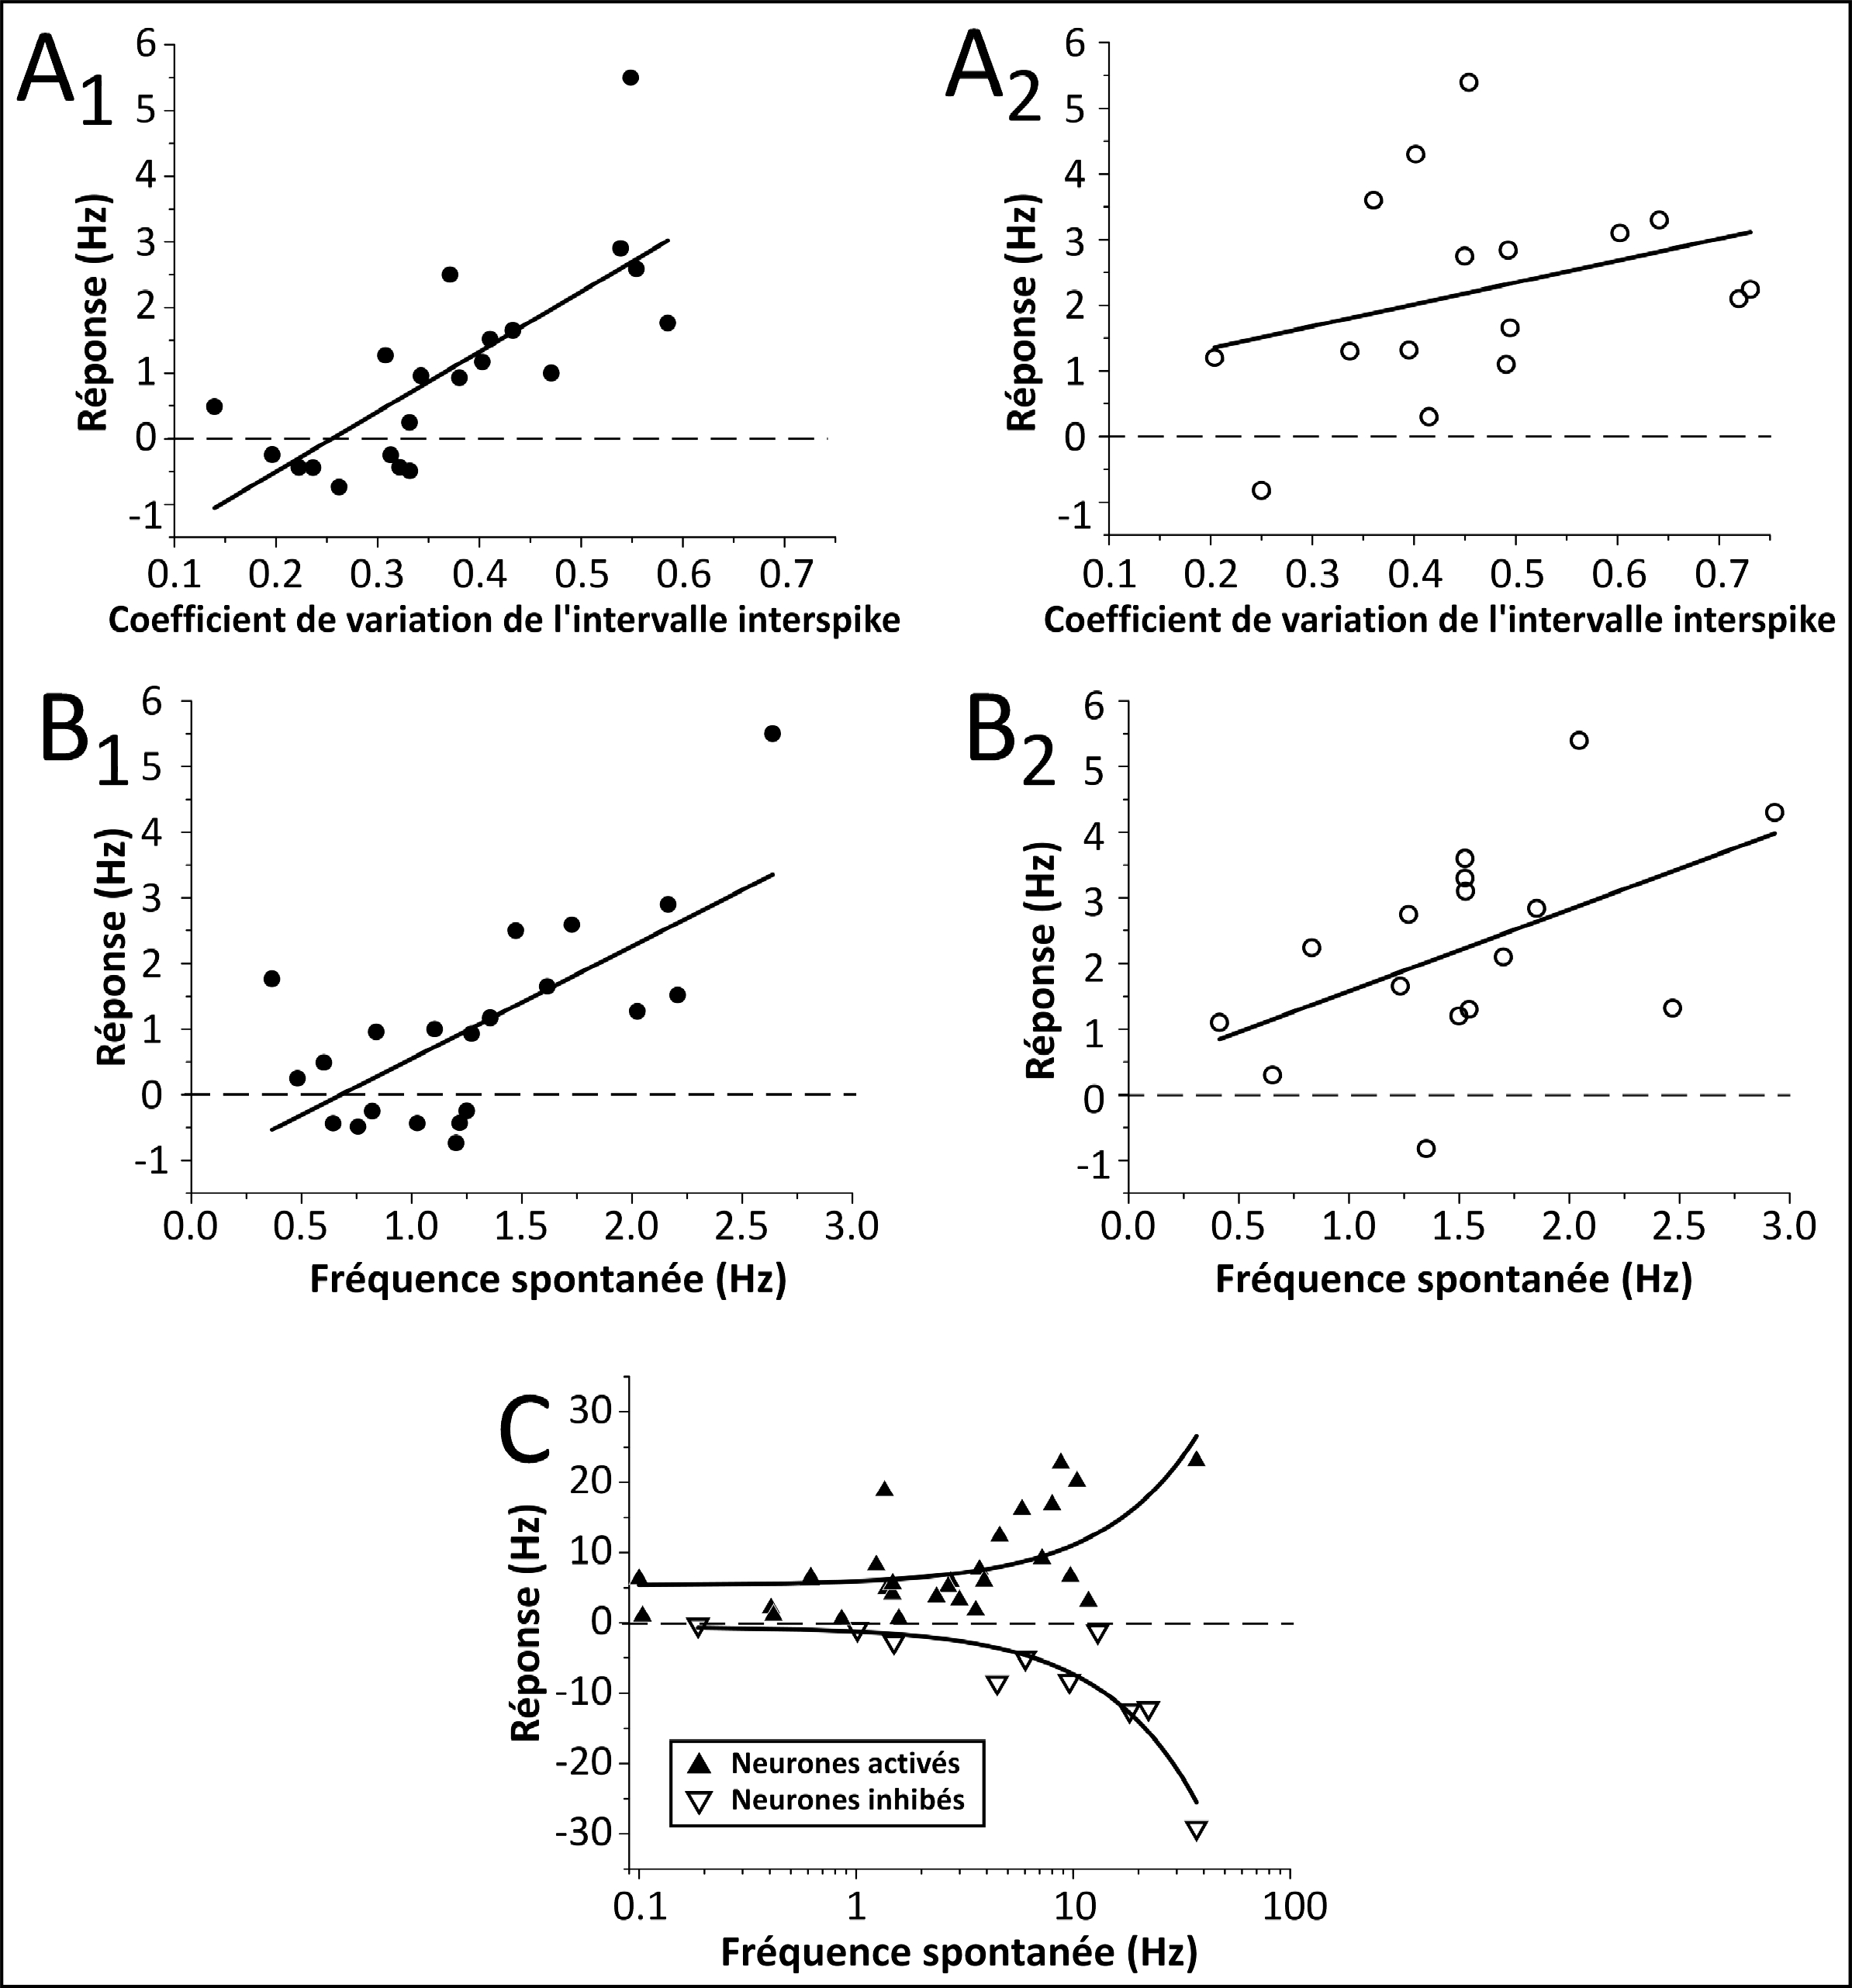
\includegraphics[width=14.5cm]{Figure12.jpg} 
\end{center}

\caption[Caractéristiques de décharge et intensité de réponse des neurones 5-HT et non-5-HT]{\textbf{Lien entre les caractéristiques de décharge des neurones sérotoninergiques et non sérotoninergiques et l’intensité de leur réponse à une stimulation nociceptive thermique}}

{\protect\parbox[t]{18cm}{
\begin{small}
\textbf{(A1)}: Lien entre la régularité de la décharge (abscisse) des neurones sérotoninergiques du RMg et l’intensité de leur réponse à des stimulations nociceptives (ordonnée) ; Régression linéaire simple : $n = 21 ; r^{2} = 0,56 ; p < 10^{-4}$ ; intervalle de confiance à 95 \% de r : 0,47-0,89.\\ 
\textbf{(A2)}: Lien entre la régularité de la décharge (abscisse) des neurones sérotoninergiques du LPGi et l’intensité de leur réponse à des stimulations nociceptives (ordonnée) ; Régression linéaire simple : $n = 16 ; r^{2} = 0,10 ; p = 0,231$ ; intervalle de confiance à 95 \% de r : -0,21-0,70.\\
\textbf{(B1)}: Lien entre la fréquence spontanée (abscisse) des neurones sérotoninergiques du RMg et l’intensité de leur réponse à des stimulations nociceptives (ordonnée) ; Régression linéaire simple : n = 21 ; $r^{2} = 0,48 ; p = 4.10^{-4}$ ; intervalle de confiance à 95 \% de r : 0,24-0,90.\\
\textbf{(B2)}: Lien entre la fréquence spontanée (abscisse) des neurones sérotoninergiques du LPGi et l’intensité de leur réponse à des stimulations nociceptives (ordonnée) ; Régression linéaire simple : n = 16 ; $r^{2} = 0,23 ; p = 0,062$ ; intervalle de confiance à 95 \% de r : -0,02-0,79.\\
\textbf{(C)}: Lien entre la fréquence spontanée (abscisse) des neurones non-sérotoninergiques de la RVM et l’intensité de leur réponse à des stimulations nociceptives (ordonnée) ; Régression linéaire simple : $n = 30 ; r^{2} = 0,37 ; p = 4.10^{-4}$ ; intervalle de confiance à 95 \% de r : 0,31-0,79 pour les neurones activés et $n = 10 ; r^{2} = 0,83 ; p = 2.10^{-4}$ ; intervalle de confiance à 95 \% de r : 0,41-0.96 pour les neurones inhibés.
\end{small}}}

\label{Figure 12}

\end{figure}

\subsection{Discussion et conclusion}

Nos résultats montrent qu’il existe un lien entre le profil de décharge spontanée des neurones sérotoninergiques du RMg et leurs réponses à des stimulations nociceptives. Un tel résultat n’avait pas été rapporté dans les études précédentes (Gao \& Mason 2000; 2001b). Toutefois, bien que non souligné dans leur article, Gao et Mason (2000) montre effectivement que les neurones sérotoninergiques du RMg inhibés par une stimulation thermique nociceptive sont plus réguliers que les neurones non répondants (voir Gao et Mason 2001 ; tableau 1 : p = 0.03). Comme mentionné précédemment (voir - discussion de l’article 3), la différence entre notre étude et les précédentes tient probablement dans le niveau d’anesthésie plus faible utilisé dans nos conditions, étant donné que les réponses des neurones de la RVM et des neurones sérotoninergiques sont affectés par l’anesthésie (Heym et al. 1984; Oliveras et al. 1991a; Oliveras et al. 1991b). On notera toutefois, que le lien entre le niveau de décharge spontanée des neurones non-sérotoninergiques et l’intensité de leur réponse à des stimuli nociceptifs, décrit précédemment (Leung \& Mason 1998), a été retrouvé dans notre étude. Ceci suggère que les réponses des neurones non-sérotoninergiques sont moins sensibles à l’anesthésie que celle des neurones sérotoninergiques.

Dans notre étude, les neurones sérotoninergiques du RMg et, dans une moindre mesure, du LPGi sont un ensemble hétérogène. Les populations, qui le composent, répondent différement à des stimuli nociceptifs. Ces populations, identifiables par leurs caractéristiques de décharge spontanée, pourraient avoir des rôles fonctionnels différents. Ces résultats sont concordants avec des données d’électrophysiologie in vivo, montrant que un tiers des neurones sérotoninergiques du RMg répondent à une injection de morphine et qu’ils se caractérisent aussi par des décharges plus irrégulières que les neurones non répondant (Gao et al. 1998). Des études \textit{in-vitro} montrent des résultats similaires (Zhang et al. 2006; Zhang \& Hammond 2010). Il est intéressant de noter que le type de réponse à la morphine des cellules sérotoninergiques du RMg est aussi associé à des différences morphologiques (i.e. arborisations dendritiques, taille du soma et degré de collatéralisation axonale), suggérant un autre critère de différenciation de ces populations (Gao \& Mason 2001b).

L’hypothèse la plus attrayante pour expliquer le lien entre les caractéristiques de décharge spontanée et l’intensité des réponses à des stimulations nociceptives est que : le pattern de décharge de ces populations de neurones est déterminé par leurs propriétés intrinsèques de membrane et que ces populations reçoivent des afférences différentes.
Le caractère régulier de la décharge spontanée des neurones sérotoninergiques du raphé dorsal est modulé par des conductances potassiques (Aghajanian \& Vandermaelen 1982b; Vandermaelen \& Aghajanian 1983; Aghajanian 1985; Haj-Dahmane et al. 1991; Bayliss et al. 1997b; Rouchet et al. 2008). Bien sûr, un tel phénomène n’exclut pas le rôle de courants entrants dans la genèse du potentiel « pacemaker » typique de ces neurones. Toutefois, un input synaptique semble nécessaire pour que certains neurones du raphé dorsal « expriment » leur irrégularité (Rouchet et al. 2008). 

Au niveau du groupe B3, les études d’électrophysiologie sur tranche examinant les courants membranaires de ces neurones les considèrent généralement comme un tout homogène, et mesurent des paramètres sur l’ensemble de la population (Bayliss et al. 1997b; 1997a). À l’inverse, les études \textit{in-vitro} qui mettent justement en avant l’hétérogénéité des profils de décharge des neurones sérotoninergiques n’étudient pas les courants potentiellement responsables de ces différences (Zhang et al. 2006; Zhang \& Hammond 2009; 2010). Néanmoins, dans le cas des neurones sérotoninergiques du RMg, les différences de pattern de décharge semblent être majoritairement dues à leurs propriétés intrinsèques de membrane, car 

\begin{itemize}
\item ces différences existent aussi dans des préparations sur tranche et donc après déafférentation, 
\item ces sous populations de neurones se retrouvent même après le blocage pharmacologique de toute activité de réseau excitatrice au sein de la tranche (Zhang \& Hammond 2010).
\end{itemize}

Malheureusement, même si certains de ces travaux \textit{in-vitro} étudient les projections de ces neurones, en associant électrophysiologie et traceurs neuronaux, ils étudient rarement les caractéristiques morphologiques (forme des somas et arborisations dendritiques) des différentes populations de neurones qu’ils mettent en évidence (Marinelli et al. 2002; Finnegan et al. 2004; Marinelli et al. 2005; Zhang et al. 2006; Zhang \& Hammond 2010). De plus, aucune étude à ce jour n’a essayé d’étudier les différences d’afférences qui pourraient exister entre ces types de neurones sérotoninergiques. Au vu de ces données, il semble donc encore difficile de conclure sur le mécanisme qui sous tend le lien entre le pattern de décharge de ces neurones et leurs réponses à des stimulations nociceptives.

De futures études d’électrophysiologie de cette région permettront d’approfondir les mécanismes et les raisons hodologiques de ce lien. De même, l’utilisation de protocoles de triple marquage permettrait de savoir si ces populations de neurones peuvent aussi être différenciées au niveau neurochimique, en fonction des neurotransmetteurs et neuropeptides qu’elles coexpriment.

\cleardoublepage

\fancyhf{} % delete current header and footer
\fancyfoot[C]{\bfseries -\thepage-}
\fancyhead[RO]{\bfseries DISCUSSION GÉNÉRALE}
\fancyhead[LE]{\bfseries DISCUSSION GÉNÉRALE}
\renewcommand{\headrulewidth}{1pt}
\renewcommand{\footrulewidth}{1pt}
\addtolength{\headheight}{1pt} % space for the rule

\part{DISCUSSION GÉNÉRALE}

\cleardoublepage

\chapter{DISCUSSION GÉNÉRALE}

\section{Rappel des principaux résultats :}

Deux des questions auxquelles nous avons cherché à répondre au cours de cette thèse portaient sur :

\begin{itemize}
\item l’origine des \textit{inputs} sérotoninergiques du NTS qui sous tendent l’inhibition de la composante cardiovagale du baroréflexe lors des réactions de défense (Article 1) ;
\item le rôle de la sérotonine et des récepteurs 5-HT$_{3}$ du NTS dans la même inhibition par des stimuli nociceptifs (Article 2).\end{itemize}

Nos résultats ont montré que, dans ces deux situations (nociception et stimulation de la dlPAG), les neurones sérotoninergiques bulbaires du groupe B3, situés au niveau du raphé magnus (RMg) et de la partie ventrale des noyaux latéraux paragigantocellulaires (LPGi), jouent un rôle clé dans ce phénomène. 

Des méthodes de double marquage immunohistochimique (c-fos + sérotonine) ont permis de montrer que seuls les neurones sérotoninergiques du groupe B3 sont activés par une stimulation de la dlPAG (Article 1), et que seuls ceux du LPGi sont activés par la plus basse température testée inhibant le baroréflexe (i.e. 48 °C) (Article 2). 

L’enregistrement électrophysiologique des neurones de cette région, associé à un marquage juxtacellulaire, a permis de clairement montrer 1) la réalité des activations de ces neurones sérotoninergiques par des stimulations nociceptives, et 2) les particularités de ceux du LPGi (Article 3).

L’activation de ces cellules par microinjection de DLH suffit aussi à inhiber le baroréflexe cardiovagal (article 1). De plus, le fait que cette inhibition est réversée par l’inactivation du groupe B3 par microinjection de muscimol, nous a permis de montrer la nécessité de l’intégrité fonctionnelle de ces neurones dans ce phénomène (Article 1 et 2). Les injections intra-NTS de granisétron permettent de lever l’inhibition du baroréflexe par un stimulus nociceptif somatique et lors de l’activation de la RVM. Ceci montre clairement le caractère sérotoninergique de cette inhibition (Article 1 et 2). 

\section{Résultats complémentaires de notre laboratoire}

Des travaux récents vont dans le même sens que ces résultats. Netzer et al. (en préparation), utilisant une même méthodologie de double immunomarquage, ont montré que l’activation du noyau cunéiformis (Cnf), qui induit les signes d’une réaction de défense et une inhibition de la composante cardiovagale du baroréflexe, active aussi les neurones du groupe B3. Le fait que cette activation est observée avec des stimulations du Cnf, aussi bien électriques que pharmacologiques, permet d’exclure le rôle de fibres de passages. De plus, l’inhibition de la bradycardie du baroréflexe par activation du Cnf est réduite après une inactivation de la dlPAG, suggérant que cette dernière relaie une partie de l’effet du Cnf. En accord avec nos résultats, Netzer et al. (en préparation) ont aussi montré que l’inactivation de la RVM permet de nettement réduire l’inhibition produite par l’activation du Cnf. Enfin, la réversion de cette inhibition par des injections de granisétron intra-NTS renforce aussi notre conclusion (Netzer et al. En préparation). 

\section{Un circuit unique impliqué dans l’inhibition du baroréflexe cardiaque}

L’ensemble de ces résultats suggère fortement que l’inhibition du baroréflexe cardiovagal par des stimulations nociceptives somatiques ou par l’activation de la dlPAG est sous-tendue par un même circuit sérotoninergique « B3-NTS ». Cette hypothèse est corroborée par le fait que ces deux types d’inhibitions impliquent des circuits très similaires au niveau du NTS. De plus, ils mettent tous les deux en jeu au niveau du NTS : les récepteurs 5-HT$_{3}$, la substance P (Boscan et al. 2002a; Pickering et al. 2003; Boscan \& Paton 2005) et in fine un mécanisme GABAergique (Nosaka et al. 1989; Sevoz-Couche et al. 2003; Comet et al. 2004; Boscan \& Paton 2005). 

Dans ces deux types d’inhibition, la sérotonine libérée active les récepteurs 5-HT$_{3}$ du NTS, dont la majorité se trouve située en position présynaptique sur les afférences vagales de ce noyau (Merahi et al. 1992b). Ces afférences étant glutamatergiques, l’activation de leurs récepteurs 5-HT$_{3}$ entraîne la libération de glutamate qui active plusieurs catégories d’interneurones du NTS (Ashworth-Preece et al. 1995; Jeggo et al. 2005). 

Certains de ces interneurones contiennent de la substance P. En effet, la microinjection intra-NTS d’antagonistes des récepteurs NK$_{1}$ de la substance P permet de bloquer ce circuit « substance Pergique », et de réduire l’inhibition de la bradycardie réflexe induite par l’activation des récepteurs 5-HT$_{3}$ ou par un stimulus nociceptif somatique (Boscan et al. 2002a; Pickering et al. 2003; Comet et al. 2005).

Une autre catégorie d’interneurones est GABAergique. Cette population d’interneurone est a priori l’effecteur final de l’inhibition de la composante cardiaque du baroréflexe au niveau du NTS (Jordan et al. 1988; Boscan \& Paton 2001; Sevoz-Couche et al. 2003). Une première partie de ces interneurones GABAergiques est directement activée par le glutamate libéré des afférences vagales, et inhibe les afférences issues des barorécepteurs carotidiens. Une deuxième partie de ces interneurones GABAergiques est indirectement activée par la libération de substance P (voir ci-dessus), et inhibe les afférences provenant des barorécepteurs aortiques (Comet et al. 2005).

\section{Généralisation : un même circuit est impliqué dans l’inhibition de la bradycardie des différents réflexes vasculaires.}

Comme mentionné dans les rappels bibliographiques (voir « \ref{Réflèxes cardiovasculaires} Les réflexes cardiovasculaires » – page \pageref{Réflèxes cardiovasculaires}), il existe, en plus du baroréflexe, deux autres réflexes qui peuvent affecter la pression artérielle à court terme : le réflexe de Bezold-Jarisch et le chémoréflexe carotidien. 

Le réflexe de Bezold-Jarisch, déclenché par l’activation de mécanorécepteurs et de chémorécepteurs cardio-pulmonaires, se caractérise par la triade de réponses suivante : bradycardie, hypotension et apnée (Aviado \& Guevara Aviado 2001). Ce réflexe est aussi appelé réflexe cardiopulmonaire, car il met en jeu deux groupes de récepteurs. Un groupe est constitué de mécano- et chémo-récepteurs localisés dans le cœur au niveau du ventricule gauche et de l’atrium. L’autre groupe de mécano- et chémo-récepteurs est situé dans les poumons (Oberg \& Thoren 1972; Donald \& Shepherd 1978; Thames et al. 1978). À l’heure actuelle, peu de choses sont connues sur le rôle physiologique de ce réflexe. Son activation pourrait expliquer les épisodes de bradycardie et d’hypotension majeurs survenant chez des patients sous anesthésie générale, ou pendant un infarctus du myocarde, pour diminuer le travail du cœur (Mark 1983). Dans le cas des infarctus du myocarde, la libération de radicaux libres ou de sérotonine, pendant la reperfusion du tissu ischémié, pourrait être à l’origine de l’activation des chémorécepteurs cardiaques (Ustinova \& Schultz 1994a; 1994b). Le réflexe de Bezold-Jarisch participerait aussi à la modulation de la pression artérielle et de la fréquence cardiaque et serait complémentaire du baroréflexe (Mancia et al. 1976; Donald \& Shepherd 1978). Une étude réalisée chez le chien a montré que le réflexe de Bezold-Jarisch joue un rôle essentiel dans l’homéostasie de la pression artérielle après ablation des barorécepteurs (Persson et al. 1988), et que sa sensibilité est accrue en cas de défaillance du baroréflexe (Alper et al. 1987).

\`A la différence du baroréflexe et de celui de Bezold-Jarisch, le chémoréflexe ne participe pas à la régulation « physiologique » de la pression artérielle basale. En effet, les chémorécepteurs, essentiellement localisés au niveau du glomus carotidien, sont sensibles aux modifications des gaz du sang (une hypoxie ou une hypercapnie). Le chémoréflexe est activé essentiellement par une diminution de la pression partielle en oxygène. La détection de cette hypoxie est responsable d’une réponse cardiovasculaire (bradycardie et augmentation de la pression artérielle) et ventilatoire (augmentation de la fréquence respiratoire). Les réponses cardiovasculaires visent d’une part à diminuer le travail du cœur et la consommation en oxygène (bradycardie) et à augmenter le débit sanguin dans les capillaires pulmonaires pour augmenter les échanges gazeux (vasoconstriction). Les fibres chémoréceptrices carotidiennes sont contenues, comme les fibres baroréceptrices carotidiennes, dans le nerf glossopharyngien qui se projette dans la région commissurale du NTS où elles induisent la libération de glutamate (Jordan \& Spyer 1986; Vardhan et al. 1993a). 

Le baroréflexe, le chémoréflexe et le réflexe de Bezold-Jarisch ont des réponses sympathiques qui varient en fonction des réflexes. Toutefois, la réponse parasympathique est commune aux trois réflexes. Celle-ci aboutit à la diminution de la fréquence cardiaque. Une étude récente a montré que le circuit « B3-NTS », décrit ci-dessus dans le cas du baroréflexe, est aussi impliqué dans l’inhibition de la bradycardie du chémoréflexe et du réflexe de Bezold-Jarisch lors d’une stimulation de la dlPAG (Netzer et al. 2009). Dans cette même étude, les auteurs ont montré que la triade « récepteur 5-HT$_{3}$ – substance P – GABA » est aussi responsable de cette inhibition au niveau du NTS.

\section{Afférences permettant l’activation du groupe B3}

Au cours de cette thèse, nous n’avons pas étudié les afférences des neurones du groupe B3, qui pourraient être directement responsables de leurs activations. Il existe cependant des données de la littérature suggérant quelques hypothèses de connections plus ou moins directes.

Concernant les afférences véhiculant les messages nociceptifs (Article 2 et 3), il faut tout d’abord rappeler que le LPGi reçoit des projections directes des couches profondes de la moelle épinière (Gallager \& Pert 1978; Abols \& Basbaum 1981; Andrezik et al. 1981). Il en est de même pour certaines des régions de la réticulée environnante, notamment latérale et gigantocellulaire (Hermann et al. 1997; Normandin \& Murphy 2008). Comme ces régions réticulaires projettent sur le RMg et le LPGi (Beitz 1982a; Lovick 1986), cela pourrait expliquer les résultats de Braz et al. (2009) qui ont, observé chez des souris transgéniques, des connections oligosynaptiques entre les neurones spinaux des couches profondes et les neurones sérotoninergiques du RMg.

La deuxième possibilité, plus probable, est que ces neurones soient indirectement activés via la voie spino-parabrachiale (Bernard et al. 1996; Gauriau \& Bernard 2002). Les principales structures de sortie de cette voie sont le noyau central de l’amygdale, l’hypothalamus ventromédian et, de manière moins marquée, la PAG (Bernard \& Besson 1990; Bester et al. 1995; Bernard et al. 1996; Bester et al. 1997). Cette possibilité offre une solution « élégante » à la question des voies neuronales permettant l’activation des neurones de la RVM. Elle permet d’une part, de faire le lien anatomique avec l’activation de ces neurones constatée lors d’une réaction de défense induite par l’activation de la dlPAG (Article 1), et d’autre part, d’expliquer certaines les différences constatées entre les neurones du LPGi et du RMg (Article 2 et 3). En effet, la principale source d’afférences de la RVM et des neurones sérotoninergiques du groupe B3 est la PAG (Abols \& Basbaum 1981; Murphy \& Hoffman 2001; Normandin \& Murphy 2008; Braz et al. 2009), qui reçoit des projections hypothalamiques. De plus, les populations de neurones de la PAG projetant sur le RMg et le LPGi ne sont pas les mêmes : la région ventrale de la PAG semblerait plus projeter sur la partie médiane de la RVM, tandis que la partie latérale de cette dernière recevrait des afférences de la colonne dorsale de la PAG (Beitz et al. 1983a; Cameron et al. 1995; Hermann et al. 1997). 

Il faut noter que ce lien, en plus d’être anatomique, est aussi fonctionnel, car la voie spino-parabrachio-amygdalienne/hypothalamique est connue pour son implication dans les réactions végétatives (le cœur de notre sujet) comme dans la nociception (Bernard et al. 1996; Boscan et al. 2005; Borszcz 2006). En effet, la stimulation de noyau parabrachial (PB) ou du noyau ventromédian de l’hypothalamus entraîne des modifications claires des paramètres cardiovasculaires, ainsi qu’une inhibition du baroréflexe (Gebber \& Snyder 1970; Coote et al. 1979; Saleh \& Connell 1997; Sevoz-Couche et al. 2003). Il faut noter que cette voie, via le PB, projette légèrement sur la RVM (Beitz 1982b; 1982a; Lovick 1986; Hermann et al. 1997). Ceci pourrait aussi contribuer aux réponses des neurones du groupe B3. De plus, l’inhibition de la bradycardie du baroréflexe par l’activation de la dlPAG pourrait être aussi, partiellement, relayée par cette structure, car cet effet de la stimulation de la dlPAG est prévenu par l’inactivation du PB (Nosaka et al. 1993; Hayward 2007). 

\section{Activation des neurones de la RVM et du groupe B3 par un variable physiologique intermédiaire}

Les stimulations (nociceptives et activations de la dlPAG) utilisées dans nos expériences affectent un ensemble de paramètres physiologiques. Ceci est valable pour le système cardiovasculaire (tachycardie et réponse pressive) et respiratoire (tachypnée).

Ainsi, il est important de savoir dans quelle mesure ces « variables intermédiaires » pourraient être responsables des changements d’activités observés dans les neurones du RMg et du LPGi avec la technique du c-fos ou l’électrophysiologie. Tout d’abord, il faut noter que, même si ces noyaux reçoivent des afférences des structures impliquées dans les régulations cardiovasculaires ou respiratoires, celles-ci sont loin d’être majeures (Lovick 1986; Hermann et al. 1997). De plus, la technique du c-fos semble montrer que peu de neurones de la RVM sont affectés par des variations des paramètres cardiovasculaires (Dampney \& Horiuchi 2003). Les données d’électrophysiologie permettent une conclusion plus définitive. Il faut ici considérer séparément le cas des neurones sérotoninergiques et celui des neurones non-sérotoninergiques. 

Dans le RMg, certains neurones sérotoninergiques semblent répondre à des augmentations de pression artérielle induites pharmacologiquement ou mécaniquement, suggérant qu’ils seraient barosensibles (Gao \& Mason 2001a). Toutefois, des études ultérieures ont montré que ce n’était pas le cas pour la grande majorité de ces neurones (Gao \& Mason 2001b). Il semble en être de même des neurones sérotoninergiques des autres raphés (RDr, ROb, RPa), qui ne répondent pas à des variations de pression (Jacobs et al. 1990; Jacobs et al. 2002). Un autre argument permet d’exclure le rôle des variables cardiovasculaires et respiratoires dans la genèse des réponses des neurones sérotoninergiques. Il vient du type de lien temporel qui existe entre les variations spontanées de l’activité de ces neurones et celles de ces paramètres physiologiques. L’activité de 80 \% des neurones sérotoninergiques du RMg est liée à des variations à très basse fréquence (avec une période à l’échelle de la dizaine de minutes) de la pression artérielle (Mason et al. 2007). En revanche, seule l’activité d’un petit nombre de ces cellules est corrélée au cycle cardiaque – de manière assez faible, suggérant que la majorité de ces neurones ne reçoit pas d’inputs barosensibles (Mason et al. 2007).

Dans le cas des cellules non-sérotoninergiques de la RVM, il existe un lien clair entre les variations à basse fréquence (période $\approx$ 8-10 min) de la pression artérielle et l’activité spontanée de ces cellules (Thurston \& Randich 1992; 1995; Leung \& Mason 1996). Toutefois, cette corrélation persiste après la dénervation des afférences baroréceptrices pour les variations spontanées de pression artérielle, mais pas pour les variations provoquées expérimentalement, montrant que ces afférences ne sont pas nécessaires à la modulation de l’activité de ces cellules (Thurston \& Randich 1995). De meme, l’activité spontanée de ces neurones n’est pas corrélée au cycle cardiaque (Leung \& Mason 1996), ce qui suggère fortement que des changement de pression artérielle ne sont pas responsables des activations observées dans notre étude d’électrophysiologie. 

Dans leur ensemble, ces résultats suggèrent que les activations observées dans nos expériences ne sont pas dues à des changements de ces variables « intermédiaires ». Pour les cellules non-sérotoninergiques, cette conclusion est renforcée par le fait que les augmentations de pression artérielle et de fréquence cardiaque induites par une stimulation nociceptive ne semblent pas nécessaires au déclenchement des réponses de ces neurones (Leung \& Mason 1998).

\bigskip 

Enfin, certains auteurs suggèrent que l’activation des neurones sérotoninergiques du RMg pourrait être plus liée à la réaction d’éveil qui accompagne la stimulation nociceptive, qu’à cette stimulation per se. En effet, chez le chat éveillé, les neurones (supposés) sérotoninergiques de ce noyau semblent répondre à tous stimuli provoquant une réaction d’éveil. De même, les réponses aux stimulations nociceptives sont plus fréquentes lorsqu’elles sont associées à une désynchronisation de l’EEG (Auerbach et al. 1985; Fornal et al. 1985)
\footnote{La question semble moins problématique pour les neurones non-sérotoninergiques car leur activation par ces stimulations est antérieure à la désynchronisation corticale (Leung \& Mason 1999).}. 
Ceci pourrait sembler problématique au premier abord. Mais cela peut se comprendre si l’on considère que ces neurones sérotoninergiques peuvent venir assister le système nerveux autonome, pour permettre une réponse coordonnée de l’organisme à une stimulation extérieure potentiellement dangereuse, particulièrement capable de déclencher une réaction d’éveil (voir ci-dessous).

\section{Conséquences physiologiques générales}

Nos résultats suggèrent que les neurones sérotoninergiques du groupe B3 augmentent leur décharge lors de situations d’urgence, dans lesquelles la survie ou l’intégrité physique de l’animal est mise en jeu, comme lors de stimulations nociceptives somatiques et lors de la réaction de défense déclenchée par une activation de la dlPAG. Pour comprendre les conséquences physiologiques de l’activation des cellules, il est nécessaire de rappeler les projections et le type de transmission qui caractérisent ces neurones. 

Tout d’abord, ces projections majoritairement descendantes contactent les neurones des couches superficielles de la moelle épinière (Bacon et al. 1990; Bowker \& Abbott 1990). Ces neurones projettent également sur les cornes intermédiolatérales. Les contacts, qu’elles y établissent avec les cellules préganglionnaires sympathiques, font que ces neurones sont connectés de façon oligosynaptique à de nombreuses cibles du système nerveux autonome, dont le cœur, les muscles impliqués dans la vasomotricité cutanée et le tissu adipeux brun, responsable de la thermogenèse non frissonnante (Loewy \& McKellar 1981; Helke et al. 1986; Appel et al. 1987; Bacon et al. 1990; Wu \& Wessendorf 1992; Haxhiu et al. 1993; Wu et al. 1993; Allen \& Cechetto 1994; Ter Horst et al. 1996; Mason 2001; Cano et al. 2003; Kerman et al. 2003; Nakamura et al. 2004b; Stornetta et al. 2004; Toth et al. 2006). 

Ensuite, les projections des neurones du groupe B3 se font au niveau du tronc : soit à un niveau local sur la RVM elle-même, soit sur d’autres structures impliquées dans le contrôle cardiovasculaire (NTS, la région ventrolatérale du bulbe [RVL]) et/ou respiratoire (noyau ambigu et noyau de Kölliker Fuse) (Holtman et al. 1984; Thor \& Helke 1987; Schaffar et al. 1988; Connelly et al. 1989; Holtman et al. 1990a; Holtman et al. 1990b; Potrebic et al. 1995; Gao \& Mason 1997; 2001b; Bago et al. 2002). 

Enfin, un même neurone sérotoninergique de cette région peut contacter plusieurs de ces structures, grâce à ses nombreuses collatérales axonales (Bowker \& Abbott 1990; Li et al. 1993b; Allen \& Cechetto 1994) et la majorité de la transmission sérotoninergique de ces neurones est de type paracrine et non synaptique (Marlier et al. 1991a; Ridet et al. 1993).

\bigskip 

Une telle organisation anatomique suggère que le rôle modulateur de ces cellules soit plus « général » que « spécifique d’une fonction donnée ». Ainsi, les neurones sérotoninergiques du groupe B3 semblent idéalement positionnés pour évaluer les conditions environnementales. Si elles le nécessitent, ils peuvent alors modifier le fonctionnement homéostatique en cours et coordonner, en fonction, la modulation de la transmission nociceptive spinale et du contrôle autonomique. 

En accord avec cette idée, l’activation des neurones de la RVM entraîne une augmentation du tonus sympathique et des changements de nombreux paramètres, tels que la pression artérielle, la fréquence cardiaque, la vascularisation cutanée, la respiration, la thermorégulation, et, bien sûr, la transmission des \textit{inputs} nociceptifs (Oliveras et al. 1975; Haselton et al. 1988; Zhuo \& Gebhart 1990; Blessing et al. 1999; Morrison et al. 1999; Blessing \& Nalivaiko 2001; Cao \& Morrison 2003; Ciriello et al. 2003; Zaretsky et al. 2003a; Nason \& Mason 2004; Ootsuka \& Blessing 2005; Cao et al. 2006; Nason \& Mason 2006). 

Certains effets, comme l’augmentation de pression artérielle ou de l’activité du tissu adipeux brun, déclenchés par l’activation de sous groupes de neurones dans les noyaux du raphé, peuvent être bloqués au niveau spinal, par des antagonistes glutamatergiques ou sérotoninergiques, suggérant l’implication de ces différentes neurotransmetteurs (McCall 1984; Nakamura et al. 2004a).

\`A l’inverse, l’inactivation de cette région peut bloquer les modulations d’un ou de plusieurs de ces paramètres par une stimulation nociceptive, un stress environnemental ou une réaction de défense (Blessing \& Nalivaiko 2000; Nalivaiko \& Blessing 2001; DiMicco et al. 2002; Zaretsky et al. 2003b; Cao et al. 2004; Vianna et al. 2008). L’implication des neurones sérotoninergiques du groupe B3 est suggérée par les expériences montrant que des injections de 8-OH-DPAT dans cette région diminuent certaines des réponses cardiovasculaires à des stress environnementaux, à des stimulations nociceptives ou à des réactions de défense induite par stimulation de l’hypothalamus dorsomédian. Ces injections peuvent aussi diminuer la réponse fébrile induite expérimentalement (Nalivaiko et al. 2005).

\bigskip 

Dans ce contexte, nos travaux montrent clairement l’implication des neurones sérotoninergiques dans l’inhibition de la bradycardie du baroréflexe, nécessaire à la réaction comportementale dans des situations d’urgence. Il faut toutefois noter que ces neurones sérotoninergiques déchargent de manière continue pendant l’éveil, mais sont silencieux pendant le sommeil (Fornal et al. 1985). Une levée de ce tonus sérotoninergique sur le NTS pourrait expliquer la facilitation du baroréflexe pendant le sommeil (Smyth et al. 1969; Sayk et al. 2007). Toutefois, l’absence d’effet sur le baroréflexe lui-même des injections intra-NTS d’antagonistes des récepteurs 5-HT$_{3}$, suggère que c’est bien la libération phasique de sérotonine qui est importante. Un autre argument en faveur d’un rôle modulateur général et phasique des neurones sérotoninergiques, est leur activation au cours de l’exercice physique, une situation pendant laquelle le baroréflexe est inhibé (Bristow et al. 1969; Veasey et al. 1995).

\section{Implications physiopathologiques potentielles}

Il est intéressant de noter que certaines situations pathologiques peuvent amener à un « dysfonctionnement » des différentes populations de neurones de la RVM, et que ce dérèglement va affecter de différentes manières les paramètres modulés par ces neurones. On peut de façon assez schématique considérer deux situations. La première situation est celle où ce dérèglement est d’origine « exogène ». Des changements plastiques auront lieu au niveau de la RVM à la suite d’une très forte augmentation des \textit{inputs} vers cette région : c’est probablement ce qui se produit lors de stimulations nociceptives prolongées ou lors des douleurs chroniques. La deuxième situation est celle où ce dérèglement est plutôt d’origine « endogène » ou « psychique » et se rapproche du trouble panique.

\bigskip 

Concernant les douleurs chroniques, de nombreuses données montrent qu’il y aurait une augmentation de l’activité descendante facilitatrice issue de la RVM et que la sérotonine jouerait un rôle important dans ce phénomène. En fait, certaines données suggèrent que, dans certaines situations de douleurs chroniques ou inflammatoires, des changements s’opèrent au niveau de la RVM. Ces modifications plastiques impliquent à la fois les neurones et les cellules gliales de cette région (Wei et al. 2008). Une des conséquences est une augmentation de l’activité de certains neurones sérotoninergiques (Miki et al. 2002; Imbe et al. 2007; Zhang \& Hammond 2010). Ainsi, cette augmentation du tonus sérotoninergique sur les récepteurs 5-HT$_{3}$ des couches superficielles des cornes dorsales est l’un des mécanismes proposés pour expliquer le rôle facilitateur de la RVM dans plusieurs modèles de douleurs chroniques (Suzuki et al. 2004a; Suzuki et al. 2005; Donovan-Rodriguez et al. 2006; Rahman et al. 2009).

Les conséquences de ces changements sur d’autres variables physiologiques ont été moins étudiées. On sait que la relation positive qui existe, chez les individus sains, entre la pression artérielle au repos et le seuil de douleur est modifiée au cours de l’installation de douleurs chronique et qu’elle tend à s’inverser. Toutefois, les mécanismes neurochimiques qui sous-tendent son fonctionnement en situation normale, et son dérèglement en condition pathologique, sont loin d’être clairs (Bruehl \& Chung 2004). De même, peu d’études ont été réalisées sur les effets à long terme des douleurs chroniques sur le contrôle cardiovasculaire. Dans des modèles de douleurs chroniques, quelques études suggèrent que les augmentations de pression artérielle et de fréquence cardiaque observées en période postopératoire diminuent par la suite, pour ne laisser qu’une variabilité augmentée du rythme cardiaque. À cela, serait associée une diminution de la sensibilité du baroréflexe (Gemes et al. 2009). Il est d’ailleurs intéressant de noter le point commun qui existe dans la temporalité des changements au niveau cardiovasculaire et au niveau nociceptif. En effet, la première phase des douleurs chroniques ne semble pas dépendre pas des \textit{inputs} facilitateurs de la RVM, tandis que l’influence de cette région serait critique pour le maintien de ces douleurs à long terme (Burgess et al. 2002).

Une partie des travaux présentés dans cette thèse a utilisé un modèle particulier de stress : la réaction de défense. Cette réaction de l’animal peut être rapprochée des attaques de panique chez les patients. Ce sont des épisodes distincts de peur intense qui se manifestent en l’absence de danger réel, et qui s’accompagnent d’une grande anxiété, de douleurs à la poitrine, de sueurs, de tremblements, d’un besoin de fuir. Le trouble panique (panic disorder) est caractérisé par une succession d’attaques de panique récurrentes et imprévisibles (Cox et al. 1994; Abbar 1996; Coll. 2006). Les travaux de Green, réalisés chez des patients éveillés, montrent que la stimulation de la dlPAG induit des signes symptomatiques des attaques de paniques (sueur, nausées, anxiété), ainsi qu’un augmentation de la pression artérielle et de la fréquence cardiaque (Green et al. 2006). 

Les patients souffrant de troubles paniques ont, par ailleurs, un risque accru de développer des pathologies cardiaques (Coryell et al. 1986; Weissman et al. 1990; Kawachi et al. 1994). En effet, ces pathologies psychiatriques sont associées à un déséquilibre de la balance cardiovagale. Un très grand nombre d’études a exploré ces altérations sympathovagales au niveau cardiaque chez ces patients (Yeragani et al. 1993; Klein et al. 1995), mais c’est essentiellement l’exacerbation du tonus sympathique qui a été étudiée (Roth et al. 1986; Stein et al. 1992; Friedman \& Thayer 1998; Barton et al. 2007; Esler et al. 2008; Baumert et al. 2009). À l’inverse, peu d’études ont été réalisées sur les conséquences des troubles paniques sur le système parasympathique et les résultats sont contradictoires. Klein et al (1995) montrent une diminution de la composante parasympathique au niveau cardiaque, alors que cette altération n’a pas été retrouvée dans d’autres études (Yeragani et al. 1993; Ito et al. 1999; Kikuchi et al. 2009). On ne peut cependant pas exclure la possibilité d’une altération de l’activité du système parasympathique cardiaque dans la genèse des altérations cardiovasculaires associées à ces pathologies. En effet, on peut supposer que l’augmentation de la composante sympathique est d’autant plus importante que le système parasympathique ne joue pas son rôle compensateur, ou que l’effet dû à la diminution du tonus cardiovagal est masqué par l’augmentation sympathique. 

Par ailleurs, l’innovation des technologies utilisées en neuroimagerie améliore les connaissances sur les structures centrales impliquées dans les troubles paniques. Ainsi, plusieurs des structures centrales étudiées chez les rongeurs semblent être aussi impliquées, chez l’être humain, dans les réponses de peur ou d’anxiété, dont le cortex préfrontal, l’amygdale, l’hippocampe, l’hypothalamus, le thalamus et la PAG (Graeff \& Del-Ben 2008). L’utilisation de l’IRM morphométrique a permis de mettre en évidence une hypertrophie de la PAG et de la région pontique chez les patients souffrant de troubles paniques (Protopopescu et al. 2006). 

Ces données sont en faveur d’une suractivation de la PAG dans ces troubles psychiatriques. Cette structure centrale est au cœur d’un circuit modulateur du système nerveux autonome et pourrait être à l’origine d’une partie des dysfonctionnements cardiaques de la balance sympathovagale associée aux troubles paniques. Dans notre modèle expérimental, nous avons montré que la PAG, activée pendant les réactions de défense, est directement à l’origine d’une inhibition de la composante cardiovagale des réflexes cardiovasculaires. Une hyperactivation chronique de cette structure centrale chez les patients atteints de troubles paniques, pourrait être à l’origine d’une altération de la composante parasympathique au niveau du cœur, parallèle à l’hyperactivation du tonus sympathique, et ainsi participer à la genèse des pathologies cardiaques. 

\section{Perspectives}

Nos résultats suggèrent que les neurones sérotoninergiques du RMg et du LPGi dans les réactions végétatives à la nociception pourraient avoir des rôles fonctionnels différents. Il existe quelques études comparatives des projections et des afférences de ces deux noyaux (Basbaum et al. 1978; Abols \& Basbaum 1981; Beitz et al. 1983a), ou des études des projections du groupe B3 dans son ensemble. Toutefois, il n’y a pas, à notre connaissance, d’étude hodologique comparative des neurones sérotoninergiques de ces deux structures. Ce type d’étude anatomique, associée au marquage de certains co-transmetteurs de la sérotonine (comme les enképhalines, le GABA ou le glutamate), permettrait d’avancer dans notre compréhension de l’hétérogénéité anatomo-fonctionnelle de ces neurones sérotoninergiques.

\bigskip 

Un deuxième axe de recherche potentiel concerne l’étude des multiples implications fonctionnelles de la sérotonine des neurones du groupe B3 et des autres neurones de la RVM. Les études portant sur ces implications ont, en général, deux grands types de limites. 

La première est liée au fait que les études cherchant à inactiver le groupe B3 ont souvent été obligées, pour des raisons méthodologiques, d’inactiver plus de neurones que ceux de ce groupe. L’utilisation de lésion électrolytique ou l’injection d’excitotoxines détruit en effet tous les neurones de cette région. De même le muscimol, qui provoque des inactivations réversibles, hyperpolarise tous les neurones. D’une façon similaire, l’injection dans la RVM de la saporine liée à des agonistes des récepteurs opioïdergiques µ, qui ne devrait détruire que les cellules « ON » des contrôles descendants de la nociception (seules, en théorie porteuses de récepteurs µ), détruit aussi probablement des cellules sérotoninergiques (certaines exprimant ces récepteurs) (Kalyuzhny et al. 1996; Marinelli et al. 2002). Le recours à des toxines spécifiques des neurones sérotoninergiques, comme la 5,7-DHT, permet de tirer des conclusions plus précises, mais reste toutefois problématique. En effet, comme nous l’avons déjà mentionné, un grand nombre de neurones sérotoninergiques du groupe B3 coexpriment d’autres neuromédiateurs ou neuromodulateurs (Hokfelt et al. 2000). En détruisant ces neurones, on va aussi supprimer un autre transmetteur ce qui empêche de conclure de manière définitive. L’utilisation du 8-OH-DPAT, a priori plus spécifique pour inhiber les neurones sérotoninergiques que le muscimol, est finalement confrontée au même problème.

La deuxième limite est liée au fait que nombre d’études précédentes n’observaient qu’une seule variable physiologique. Ce constat est particulièrement clair pour les travaux qui portent sur le rôle de la RVM et de ses neurones sérotoninergiques dans les contrôles descendants de la nociception. Les études des effets « végétatifs » de cette région examinent plus souvent les variations de plusieurs paramètres (cardiovasculaires et thermorégulations).

\bigskip 

Nous nous proposons de faire une étude en prenant au mieux en compte les limites des travaux précédents. Pour étudier le rôle spécifique de la sérotonine sans détruire les neurones sérotoninergiques, et les autres neuro-modulateurs/transmetteurs que certains d’entre eux expriment, nous souhaitons inactiver la synthèse de sérotonine de ces neurones par injection dans la RVM de lentivirus contenant des ARN interférents spécifiques de la TPH2 et un ARNm de la GFP. Des révélations en immunohistofluorescence (GFP + TPH2) nous permettront de quantifier l’étendue de la zone infectée et la proportion de neurones sérotoninergiques dépourvus de TPH2. La diminution de sérotonine au niveau spinal sera quantifiée par chromatographie. 

Les effets de ces ARN interférents sur plusieurs paramètres physiologiques seront comparés à ceux d’un ARN contrôle. Tout d’abord, nous évaluerons les conséquences sur la nociception aiguë avec différents types de tests et dans plusieurs modalités (test de Von Frey, Randal et Sélito, Hot plate…), mais aussi dans des modèles de douleurs chroniques, comme après constriction d’un nerf. Ensuite, nous quantifierons les capacités motrices de ces animaux sur des tests d’actimétrie et de rotarod. Les effets sur plusieurs paramètres (respiration, EEG) seront aussi analysés au cours du cycle veille-sommeil. Enfin, nous analyserons les réponses cardiovasculaires de ces animaux à des stimulations nociceptives : augmentation de pression artérielle, de fréquence cardiaque et inhibition des bradycardies des différents réflexes cardiovasculaires.

\bigskip 

Ces deux axes de recherche devraient permettre d’éclaircir le rôle des différentes populations de neurones de la RVM dans tout un ensemble de régulations physiologiques.

\cleardoublepage

\fancyhf{} % delete current header and footer
\fancyfoot[C]{\bfseries -\thepage-}
\fancyhead[C]{\bfseries BIBLIOGRAPHIE}
\renewcommand{\headrulewidth}{1pt}
\renewcommand{\footrulewidth}{1pt}
\addtolength{\headheight}{1pt} % space for the rule

\part{BIBLIOGRAPHIE}

\setlength{\parindent}{-0.3cm}
\setlength{\columnsep}{1cm}

\twocolumn

\begin{singlespacing}
\begin{footnotesize}

\medskip 
\begin{Large}\textbf{A}\end{Large}

Abbar, M. (1996). Panic disorder and panic attack. Encephale, 22 Spec No 5, 13-18.

Abols, I. A. \& Basbaum, A. I. (1981). Afferent connections of the rostral medulla of the cat: a neural substrate for midbrain-medullary interactions in the modulation of pain. J Comp Neurol, 201(2), 285-297.

Aghajanian, G. K. (1985). Modulation of a transient outward current in serotonergic neurones by \linebreak alpha 1-adrenoceptors. Nature, 315(6019), 501-503.

Aghajanian, G. K. \& Vandermaelen, C. P. (1982a). Intracellular identification of central noradrenergic and serotonergic neurons by a new double labeling procedure. J Neurosci, 2(12), 1786-1792.

Aghajanian, G. K. \& Vandermaelen, C. P. (1982b). Intracellular recordings from serotonergic dorsal raphe neurons: pacemaker potentials and the effect of LSD. Brain Res, 238(2), 463-469.

Aicher, S. A., Kurucz, O. S., Reis, D. J. \& Milner, T. A. (1995). Nucleus tractus solitarius efferent terminals synapse on neurons in the caudal ventrolateral medulla that project to the rostral ventrolateral medulla. Brain Res, 693(1-2), 51-63.

Akil, H. \& Liebeskind, J. C. (1975). Monoaminergic mechanisms of stimulation-produced analgesia. Brain Res, 94(2), 279-296.

Akil, H. \& Mayer, D. J. (1972). Antagonism of stimulation-produced analgesia by p-CPA, a serotonin synthesis inhibitor. Brain Res, 44(2), 692-697.

Akil, H., Mayer, D. J. \& Liebeskind, J. C. (1972). Comparison in the rat between analgesia induced by stimulation of periacqueducal gray matter and morphine analgesia. C R Acad Sci Hebd Seances Acad Sci D, 274(26), 3603-3605.

Akil, H., Mayer, D. J. \& Liebeskind, J. C. (1976). Antagonism of stimulation-produced analgesia by naloxone, a narcotic antagonist. Science, 191(4230), 961-962.

Alhaider, A. A., Lei, S. Z. \& Wilcox, G. L. (1991). Spinal 5-HT$_{3}$ receptor-mediated antinociception: possible release of GABA. J Neurosci, 11(7), 1881-1888.

Ali, Z., Wu, G., Kozlov, A. \& Barasi, S. (1996). The role of 5HT3 in nociceptive processing in the rat spinal cord: results from behavioural and electrophysiological studies. Neurosci Lett, 208(3), 203-207.

Allen, G. V. \& Cechetto, D. F. (1994). Serotoninergic and nonserotoninergic neurons in the medullary raphe system have axon collateral projections to autonomic and somatic cell groups in the medulla and spinal cord. J Comp Neurol, 350(3), 357-366.

Allers, K. A. \& Sharp, T. (2003). Neurochemical and anatomical identification of fast- and slow-firing neurones in the rat dorsal raphe nucleus using juxtacellular labelling methods in vivo. Neuroscience, 122(1), 193-204.

Alloui, A., Chassaing, C., Schmidt, J., Ardid, D., Dubray, C., Cloarec, A. \& Eschalier, A. (2002). Paracetamol exerts a spinal, tropisetron-reversible, antinociceptive effect in an inflammatory pain model in rats. Eur J Pharmacol, 443(1-3), 71-77.

Alper, R. H., Jacob, H. J. \& Brody, M. J. (1987). Regulation of arterial pressure lability in rats with chronic sinoaortic deafferentation. Am J Physiol, 253(2 Pt 2), H466-474.

Andrezik, J. A., Chan-Palay, V. \& Palay, S. L. (1981). The nucleus paragigantocellularis lateralis in the rat. Demonstration of afferents by the retrograde transport of horseradish peroxidase. Anat Embryol (Berl), 161(4), 373-390.

Antal, M., Petko, M., Polgar, E., Heizmann, C. W. \& Storm-Mathisen, J. (1996). Direct evidence of an extensive GABAergic innervation of the spinal dorsal horn by fibres descending from the rostral ventromedial medulla. Neuroscience, 73(2), 509-518.

Antunes, V. R. \& Machado, B. H. (2003). Antagonism of glutamatergic metabotropic receptors in the NTS of awake rats does not affect the gain of the baroreflex. Auton Neurosci, 103(1-2), 65-71.

Apkarian, A. V., Bushnell, M. C., Treede, R. D. \& Zubieta, J. K. (2005). Human brain mechanisms of pain perception and regulation in health and disease. Eur J Pain, 9(4), 463-484.

Appel, N. M., Wessendorf, M. W. \& Elde, R. P. (1987). Thyrotropin-releasing hormone in spinal cord: coexistence with serotonin and with substance P in fibers and terminals apposing identified preganglionic sympathetic neurons. Brain Res, 415(1), 137-143.

Arvidsson, U., Cullheim, S., Ulfhake, B., Bennett, G. W., Fone, K. C., Cuello, A. C., Verhofstad, A. A., Visser, T. J. \& Hokfelt, T. (1990). 5-Hydroxytryptamine, substance P, and thyrotropin-releasing hormone in the adult cat spinal cord segment L7: immunohistochemical and chemical studies. Synapse, 6(3), 237-270.

Arvidsson, U., Cullheim, S., Ulfhake, B., Luppi, P. H., Kitahama, K., Jouvet, M. \& Hokfelt, T. (1994). Quantitative and qualitative aspects on the distribution of 5-HT and its coexistence with substance P and TRH in cat ventral medullary neurons. J Chem Neuroanat, 7(1-2), 3-12.

Arvidsson, U., Dado, R. J., Riedl, M., Lee, J. H., Law, P. Y., Loh, H. H., Elde, R. \& Wessendorf, M. W. (1995a). delta-Opioid receptor immunoreactivity: distribution in brainstem and spinal cord, and relationship to biogenic amines and enkephalin. J Neurosci, 15(2), 1215-1235.

Arvidsson, U., Riedl, M., Chakrabarti, S., Lee, J. H., Nakano, A. H., Dado, R. J., Loh, H. H., Law, P. Y., Wessendorf, M. W. \& Elde, R. (1995b). Distribution and targeting of a mu-opioid receptor (MOR1) in brain and spinal cord. J Neurosci, 15(5 Pt 1), 3328-3341.

Arvieu, L., Mauborgne, A., Bourgoin, S., Oliver, C., Feltz, P., Hamon, M. \& Cesselin, F. (1996). Sumatriptan inhibits the release of CGRP and substance P from the rat spinal cord. Neuroreport, 7(12), 1973-1976.

Ashworth-Preece, M. A., Jarrott, B. \& Lawrence, A. J. (1995). 5-Hydroxytryptamine3 receptor modulation of excitatory amino acid release in the rat nucleus tractus solitarius. Neurosci Lett, 191(1-2), 75-78.

Auerbach, S., Fornal, C. \& Jacobs, B. L. (1985). Response of serotonin-containing neurons in nucleus raphe magnus to morphine, noxious stimuli, and periaqueductal gray stimulation in freely moving cats. Exp Neurol, 88(3), 609-628.

Aviado, D. M. \& Guevara Aviado, D. (2001). The Bezold-Jarisch reflex. A historical perspective of cardiopulmonary reflexes. Ann N Y Acad Sci, 940, 48-58.

Aylwin, M. L., Horowitz, J. M. \& Bonham, A. C. (1997). NMDA receptors contribute to primary visceral afferent transmission in the nucleus of the solitary tract. J Neurophysiol, 77(5), 2539-2548.

Azami, J., Llewelyn, M. B. \& Roberts, M. H. (1982). The contribution of nucleus reticularis paragigantocellularis and nucleus raphe magnus to the analgesia produced by systemically administered morphine, investigated with the microinjection technique. Pain, 12(3), 229-246.

\medskip
\begin{Large}\textbf{B}\end{Large}

Bacon, S. J., Zagon, A. \& Smith, A. D. (1990). Electron microscopic evidence of a monosynaptic pathway between cells in the caudal raphe nuclei and sympathetic preganglionic neurons in the rat spinal cord. Exp Brain Res, 79(3), 589-602.

Baez, M. A., Brink, T. S. \& Mason, P. (2005). Roles for pain modulatory cells during micturition and continence. J Neurosci, 25(2), 384-394.

Bago, M., Marson, L. \& Dean, C. (2002). Serotonergic projections to the rostroventrolateral medulla from midbrain and raphe nuclei. Brain Res, 945(2), 249-258.

Bandler, R., Keay, K. A., Floyd, N. \& Price, J. (2000). Central circuits mediating patterned autonomic activity during active vs. passive emotional coping. Brain Res Bull, 53(1), 95-104.

Bandler, R. \& Shipley, M. T. (1994). Columnar organization in the midbrain periaqueductal gray: modules for emotional expression? Trends Neurosci, 17(9), 379-389.

Bannister, K., Bee, L. A. \& Dickenson, A. H. (2009). Preclinical and early clinical investigations related to monoaminergic pain modulation. Neurotherapeutics, 6(4), 703-712.

Barbaro, N. M., Hammond, D. L. \& Fields, H. L. (1985). Effects of intrathecally administered methysergide and yohimbine on microstimulation-produced antinociception in the rat. Brain Res, 343(2), 223-229.

Barbaro, N. M., Heinricher, M. M. \& Fields, H. L. (1986). Putative pain modulating neurons in the rostral ventral medulla: reflex-related activity predicts effects of morphine. Brain Res, 366(1-2), 203-210.

Barbaro, N. M., Heinricher, M. M. \& Fields, H. L. (1989). Putative nociceptive modulatory neurons in the rostral ventromedial medulla of the rat display highly correlated firing patterns. Somatosens Mot Res, 6(4), 413-425.

Bardin, L., Bardin, M., Lavarenne, J. \& Eschalier, A. (1997a). Effect of intrathecal serotonin on nociception in rats: influence of the pain test used. Exp Brain Res, 113(1), 81-87.

Bardin, L., Jourdan, D., Alloui, A., Lavarenne, J. \& Eschalier, A. (1997b). Differential influence of two serotonin 5-HT$_{3}$ receptor antagonists on spinal serotonin-induced analgesia in rats. Brain Res, 765(2), 267-272.

Bardin, L., Lavarenne, J. \& Eschalier, A. (2000). Serotonin receptor subtypes involved in the spinal antinociceptive effect of 5-HT in rats. Pain, 86(1-2), 11-18.

Barnes, N. M. \& Sharp, T. (1999). A review of central 5-HT receptors and their function. Neuropharmacology, 38(8), 1083-1152.

Barton, D. A., Dawood, T., Lambert, E. A., Esler, M. D., Haikerwal, D., Brenchley, C., Socratous, F., Kaye, D. M., Schlaich, M. P., Hickie, I. \& Lambert, G. W. (2007). Sympathetic activity in major depressive disorder: identifying those at increased cardiac risk? J Hypertens, 25(10), 2117-2124.

Basbaum, A. I., Bautista, D. M., Scherrer, G. \& Julius, D. (2009). Cellular and molecular mechanisms of pain. Cell, 139(2), 267-284.

Basbaum, A. I., Clanton, C. H. \& Fields, H. L. (1978). Three bulbospinal pathways from the rostral medulla of the cat: an autoradiographic study of pain modulating systems. J Comp Neurol, 178(2), 209-224.

Basbaum, A. I. \& Fields, H. L. (1978). Endogenous pain control mechanisms: review and hypothesis. Ann Neurol, 4(5), 451-462.

Basbaum, A. I. \& Fields, H. L. (1984). Endogenous pain control systems: brainstem spinal pathways and endorphin circuitry. Annu Rev Neurosci, 7, 309-338.

Basbaum, A. I. \& Jessell, T. M. i. e.,,). ( 2000). The perception of pain. In Kandel, Schwartz \& Jessell (Eds.), Principles of Neuroscience (4th ed., pp. 472-491). New York: McGraw-Hill.

Basbaum, A. I., Zahs, K., Lord, B. \& Lakos, S. (1988). The fiber caliber of 5-HT immunoreactive axons in the dorsolateral funiculus of the spinal cord of the rat and cat. Somatosens Res, 5(3), 177-185.

Baude, A. \& Shigemoto, R. (1998). Cellular and subcellular distribution of substance P receptor immunoreactivity in the dorsal vagal complex of the rat and cat: a light and electron microscope study. J Comp Neurol, 402(2), 181-196.

Baumert, M., Lambert, G. W., Dawood, T., Lambert, E. A., Esler, M. D., McGrane, M., Barton, D., Sanders, P. \& Nalivaiko, E. (2009). Short-term heart rate variability and cardiac norepinephrine spillover in patients with depression and panic disorder. Am J Physiol Heart Circ Physiol, 297(2), H674-679.

Bautista, D. M., Jordt, S. E., Nikai, T., Tsuruda, P. R., Read, A. J., Poblete, J., Yamoah, E. N., Basbaum, A. I. \& Julius, D. (2006). TRPA1 mediates the inflammatory actions of environmental irritants and proalgesic agents. Cell, 124(6), 1269-1282.

Bautista, D. M., Siemens, J., Glazer, J. M., Tsuruda, P. R., Basbaum, A. I., Stucky, C. L., Jordt, S. E. \& Julius, D. (2007). The menthol receptor TRPM8 is the principal detector of environmental cold. Nature, 448(7150), 204-208.

Bayliss, D. A., Li, Y. W. \& Talley, E. M. (1997a). Effects of serotonin on caudal raphe neurons: activation of an inwardly rectifying potassium conductance. J Neurophysiol, 77(3), 1349-1361.

Bayliss, D. A., Li, Y. W. \& Talley, E. M. (1997b). Effects of serotonin on caudal raphe neurons: inhibition of N- and P/Q-type calcium channels and the afterhyperpolarization. J Neurophysiol, 77(3), 1362-1374.

Bederson, J. B., Fields, H. L. \& Barbaro, N. M. (1990). Hyperalgesia during naloxone-precipitated withdrawal from morphine is associated with increased on-cell activity in the rostral ventromedial medulla. Somatosens Mot Res, 7(2), 185-203.

Bee, L. A. \& Dickenson, A. H. (2007). Rostral ventromedial medulla control of spinal sensory processing in normal and pathophysiological states. Neuroscience, 147(3), 786-793.

Bee, L. A. \& Dickenson, A. H. (2008). Descending facilitation from the brainstem determines behavioural and neuronal hypersensitivity following nerve injury and efficacy of pregabalin. Pain, 140(1), 209-223.

Behbehani, M. M. \& Fields, H. L. (1979). Evidence that an excitatory connection between the periaqueductal gray and nucleus raphe magnus mediates stimulation produced analgesia. Brain Res, 170(1), 85-93.

Beitz, A. J. (1982a). The nuclei of origin of brain stem enkephalin and substance P projections to the rodent nucleus raphe magnus. Neuroscience, 7(11), 2753-2768.

Beitz, A. J. (1982b). The sites of origin brain stem neurotensin and serotonin projections to the rodent nucleus raphe magnus. J Neurosci, 2(7), 829-842.

Beitz, A. J., Mullett, M. A. \& Weiner, L. L. (1983a). The periaqueductal gray projections to the rat spinal trigeminal, raphe magnus, gigantocellular pars alpha and paragigantocellular nuclei arise from separate neurons. Brain Res, 288(1-2), 307-314.

Beitz, A. J., Shepard, R. D. \& Wells, W. E. (1983b). The periaqueductal gray-raphe magnus projection contains somatostatin, neurotensin and serotonin but not cholecystokinin. Brain Res, 261(1), 132-137.

Belcher, G., Ryall, R. W. \& Schaffner, R. (1978). The differential effects of 5-hydroxytryptamine, noradrenaline and raphe stimulation on nociceptive and non-nociceptive dorsal horn interneurones in the cat. Brain Res, 151(2), 307-321.

Bennett, G. J. \& Mayer, D. J. (1979). Inhibition of spinal cord interneurons by narcotic microinjection and focal electrical stimulation in the periaqueductal central gray matter. Brain Res, 172(2), 243-257.

Berendse, H. W. \& Groenewegen, H. J. (1991). Restricted cortical termination fields of the midline and intralaminar thalamic nuclei in the rat. Neuroscience, 42(1), 73-102.

Bernard, J. F. \& Besson, J. M. (1990). The spino(trigemino)\linebreak pontoamygdaloid pathway: electrophysiological evidence for an involvement in pain processes. J Neurophysiol, 63(3), 473-490.

Bernard, J. F., Bester, H. \& Besson, J. M. (1996). Involvement of the spino-parabrachio -amygdaloid and -hypothalamic pathways in the autonomic and affective emotional aspects of pain. Prog Brain Res, 107, 243-255.

Bernard, J. F., Dallel, R., Raboisson, P., Villanueva, L. \& Le Bars, D. (1995). Organization of the efferent projections from the spinal cervical enlargement to the parabrachial area and periaqueductal gray: a PHA-L study in the rat. J Comp Neurol, 353(4), 480-505.

Bernard, J. F., Huang, G. F. \& Besson, J. M. (1994). The parabrachial area: electrophysiological evidence for an involvement in visceral nociceptive processes. J Neurophysiol, 71(5), 1646-1660.

Bernard, J. F., Netzer, F., Gau, R., Hamon, M., Laguzzi, R. \& Sevoz-Couche, C. (2008). Critical role of B3 serotonergic cells in baroreflex inhibition during the defense reaction triggered by dorsal periaqueductal gray stimulation. J Comp Neurol, 506(1), 108-121.

Bernard, J. F., Peschanski, M. \& Besson, J. M. (1989). Afferents and efferents of the rat cuneiformis nucleus: an anatomical study with reference to pain transmission. Brain Res, 490(1), 181-185.

Bernard, J. F. \& Villanueva, L. (2009). Architecture fonctionelle des systèmes nociceptifs. In Bouhassira \& Calvino (Eds.), Douleurs : Physiologie, physiopathologie, et pharmacologie. Paris: Arnette.

Bernard, J. F., Villanueva, L., Carroue, J. \& Le Bars, D. (1990). Efferent projections from the subnucleus reticularis dorsalis (SRD): a Phaseolus vulgaris leucoagglutinin study in the rat. Neurosci Lett, 116(3), 257-262.

Berthier, M., Starkstein, S. \& Leiguarda, R. (1988). Asymbolia for pain: a sensory-limbic disconnection syndrome. Ann Neurol, 24(1), 41-49.

Besson, J. M. \& Chaouch, A. (1987). Peripheral and spinal mechanisms of nociception. Physiol Rev, 67(1), 67-186.

Bessou, P., Burgess, P. R., Perl, E. R. \& Taylor, C. B. (1971). Dynamic properties of mechanoreceptors with unmyelinated (C) fibers. J Neurophysiol, 34(1), 116-131.

Bessou, P. \& Perl, E. R. (1969). Response of cutaneous sensory units with unmyelinated fibers to noxious stimuli. J Neurophysiol, 32(6), 1025-1043.

Bester, H., Besson, J. M. \& Bernard, J. F. (1997). Organization of efferent projections from the parabrachial area to the hypothalamus: a Phaseolus vulgaris-\linebreak leucoagglutinin study in the rat. J Comp Neurol, 383(3), 245-281.

Bester, H., Bourgeais, L., Villanueva, L., Besson, J. M. \& Bernard, J. F. (1999). Differential projections to the intralaminar and gustatory thalamus from the parabrachial area: a PHA-L study in the rat. J Comp Neurol, 405(4), 421-449.

Bester, H., Chapman, V., Besson, J. M. \& Bernard, J. F. (2000). Physiological properties of the lamina I spinoparabrachial neurons in the rat. J Neurophysiol, 83(4), 2239-2259.

Bester, H., Menendez, L., Besson, J. M. \& Bernard, J. F. (1995). Spino (trigemino) parabrachiohypothalamic pathway: electrophysiological evidence for an involvement in pain processes. J Neurophysiol, 73(2), 568-585.

Bhaskaran, D. \& Freed, C. R. (1988). Changes in arterial blood pressure lead to baroreceptor-mediated changes in norepinephrine and 5-hydroxyindoleacetic acid in rat nucleus tractus solitarius. J Pharmacol Exp Ther, 245(1), 356-363.

Bineau-Thurotte, M., Godefroy, F., Weil-Fugazza, J. \& Besson, J. M. (1984). The effect of morphine on the potassium evoked release of tritiated 5-hydroxytryptamine from spinal cord slices in the rat. Brain Res, 291(2), 293-299.

Blessing, W. W. (2004). 5-hydroxytryptamine 1A receptor activation reduces cutaneous vasoconstriction and fever associated with the acute inflammatory response in rabbits. Neuroscience, 123(1), 1-4.

Blessing, W. W. \& Nalivaiko, E. (2000). Regional blood flow and nociceptive stimuli in rabbits: patterning by medullary raphe, not ventrolateral medulla. J Physiol, 524 Pt 1, 279-292.

Blessing, W. W. \& Nalivaiko, E. (2001). Raphe magnus-\linebreak pallidus neurons regulate tail but not mesenteric arterial blood flow in rats. Neuroscience, 105(4), 923-929.

Blessing, W. W., Yu, Y. H. \& Nalivaiko, E. (1999). Raphe pallidus and parapyramidal neurons regulate ear pinna vascular conductance in the rabbit. Neurosci Lett, 270(1), 33-36.

Blinder, K. J., Gatti, P. J., Johnson, T. A., Lauenstein, J. M., Coleman, W. P., Gray, A. L. \& Massari, V. J. (1998). Ultrastructural circuitry of cardiorespiratory reflexes: there is a monosynaptic path between the nucleus of the solitary tract and vagal preganglionic motoneurons controlling atrioventricular conduction in the cat. Brain Res, 785(1), 143-157.

Bodnar, R. J., Williams, C. L., Lee, S. J. \& Pasternak, G. W. (1988). Role of mu 1-opiate receptors in supraspinal opiate analgesia: a microinjection study. Brain Res, 447(1), 25-34.

Boess, F. G. \& Martin, I. L. (1994). Molecular biology of 5-HT receptors. Neuropharmacology, 33(3-4), 275-317.

Bonagamba, L. G., Sevoz-Couche, C., N'Diaye, A., Uygun-Louvet, K., Callera, J., Machado, B. H., Hamon, M. \& Laguzzi, R. (2000). Bradycardic responses to microinjection of N-methyl-D-aspartate into the nucleus tractus solitarius are inhibited by local activation of 5-HT(3) receptors. Neuropharmacology, 39(12), 2336-2345.

Bonnavion, P., Bernard, J. F., Hamon, M., Adrien, J. \& Fabre, V. (2010). Heterogeneous distribution of the serotonin 5-HT(1A) receptor mRNA in chemically identified neurons of the mouse rostral brainstem: Implications for the role of serotonin in the regulation of wakefulness and REM sleep. J Comp Neurol, 518(14), 2744-2770.

Bonnefont, J., Chapuy, E., Clottes, E., Alloui, A. \& Eschalier, A. (2005). Spinal 5-HT$_{1A}$ receptors differentially influence nociceptive processing according to the nature of the noxious stimulus in rats: effect of WAY-100635 on the antinociceptive activities of paracetamol, venlafaxine and 5-HT. Pain, 114(3), 482-490.

Boothman, L., Raley, J., Denk, F., Hirani, E. \& Sharp, T. (2006). In vivo evidence that 5-HT(2C) receptors inhibit 5-HT neuronal activity via a GABAergic mechanism. Br J Pharmacol, 149(7), 861-869.

Borszcz, G. S. (2006). Contribution of the ventromedial hypothalamus to generation of the affective dimension of pain. Pain, 123(1-2), 155-168.

Boscan, P., Dutschmann, M., Herbert, H. \& Paton, J. F. (2005). Neurokininergic mechanism within the lateral crescent nucleus of the parabrachial complex participates in the heart-rate response to nociception. J Neurosci, 25(6), 1412-1420.

Boscan, P., Kasparov, S. \& Paton, J. F. (2002a). Somatic nociception activates NK$_{1}$ receptors in the nucleus tractus solitarii to attenuate the baroreceptor cardiac reflex. Eur J Neurosci, 16(5), 907-920.

Boscan, P. \& Paton, J. F. (2001). Role of the solitary tract nucleus in mediating nociceptive evoked cardiorespiratory responses. Auton Neurosci, 86(3), 170-182.

Boscan, P. \& Paton, J. F. (2005). Excitatory convergence of periaqueductal gray and somatic afferents in the solitary tract nucleus: role for neurokinin 1 receptors. Am J Physiol Regul Integr Comp Physiol, 288(1), R262-269.

Boscan, P., Pickering, A. E. \& Paton, J. F. (2002b). The nucleus of the solitary tract: an integrating station for nociceptive and cardiorespiratory afferents. Exp Physiol, 87(2), 259-266.

Bouhassira, D., Bing, Z. \& Le Bars, D. (1990). Studies of the brain structures involved in diffuse noxious inhibitory controls: the mesencephalon. J Neurophysiol, 64(6), 1712-1723.

Bouhassira, D., Bing, Z. \& Le Bars, D. (1992a). Effects of lesions of locus coeruleus/subcoeruleus on diffuse noxious inhibitory controls in the rat. Brain Res, 571(1), 140-144.

Bouhassira, D., Bing, Z. \& Le Bars, D. (1993a). Studies of brain structures involved in diffuse noxious inhibitory controls in the rat: the rostral ventromedial medulla. J Physiol, 463, 667-687.

Bouhassira, D., Chitour, D., Villanueva, L. \& Le Bars, D. (1993b). Morphine and diffuse noxious inhibitory controls in the rat: effects of lesions of the rostral ventromedial medulla. Eur J Pharmacol, 232(2-3), 207-215.

Bouhassira, D., Le Bars, D. \& Villanueva, L. (1987). Heterotopic activation of A delta and C fibres triggers inhibition of trigeminal and spinal convergent neurones in the rat. J Physiol, 389, 301-317.

Bouhassira, D., Villanueva, L., Bing, Z. \& le Bars, D. (1992b). Involvement of the subnucleus reticularis dorsalis in diffuse noxious inhibitory controls in the rat. Brain Res, 595(2), 353-357.

Bourgoin, S., Oliveras, J. L., Bruxelle, J., Hamon, M. \& Besson, J. M. (1980). Electrical stimulation of the nucleus raphe magnus in the rat. Effects on 5-HT metabolism in the spinal cord. Brain Res, 194(2), 377-389.

Bousquet, P., Feldman, J., Bloch, R. \& Schwartz, J. (1982). Evidence for a neuromodulatory role of GABA at the first synapse of the baroreceptor reflex pathway. Effects of GABA derivatives injected into the NTS. Naunyn Schmiedebergs Arch Pharmacol, 319(2), 168-171.

Bowker, R. M. \& Abbott, L. C. (1990). Quantitative re-evaluation of descending serotonergic and non-\linebreak serotonergic projections from the medulla of the rodent: evidence for extensive co-existence of serotonin and peptides in the same spinally projecting neurons, but not from the nucleus raphe magnus. Brain Res, 512(1), 15-25.

Bowker, R. M. \& Dilts, R. P. (1988). Distribution of mu-opioid receptors in the nucleus raphe magnus and nucleus gigantocellularis: a quantitative autoradiographic study. Neurosci Lett, 88(3), 247-252.

Bowsher, D. (1976). Role of the reticular formation in responses to noxious stimulation. Pain, 2(4), 361-378.

Bradley, P. B., Engel, G., Feniuk, W., Fozard, J. R., Humphrey, P. P., Middlemiss, D. N., Mylecharane, E. J., Richardson, B. P. \& Saxena, P. R. (1986). Proposals for the classification and nomenclature of functional receptors for 5-hydroxytryptamine. Neuropharmacology, 25(6), 563-576.

Braz, J. M., Enquist, L. W. \& Basbaum, A. I. (2009). Inputs to serotonergic neurons revealed by conditional viral transneuronal tracing. J Comp Neurol, 514(2), 145-160.

Braz, J. M., Nassar, M. A., Wood, J. N. \& Basbaum, A. I. (2005). Parallel "pain" pathways arise from subpopulations of primary afferent nociceptor. Neuron, 47(6), 787-793.

Brenchat, A., Nadal, X., Romero, L., Ovalle, S., Muro, A., Sanchez-Arroyos, R., Portillo-Salido, E., Pujol, M., Montero, A., Codony, X., Burgueno, J., Zamanillo, D., Hamon, M., Maldonado, R. \& Vela, J. M. (2010). Pharmacological activation of 5-HT(7) receptors reduces nerve injury-induced mechanical and thermal hypersensitivity. Pain, 149(3), 483-494.

Brink, T. S. \& Mason, P. (2003). Raphe magnus neurons respond to noxious colorectal distension. J Neurophysiol, 89(5), 2506-2515.

Brischoux, F., Chakraborty, S., Brierley, D. I. \& Ungless, M. A. (2009). Phasic excitation of dopamine neurons in ventral VTA by noxious stimuli. Proc Natl Acad Sci U S A, 106(12), 4894-4899.

Bristow, J. D., Brown, E. B., Jr., Cunningham, D. J., Goode, R. C., Howson, M. G., Pickering, T. G. \& Sleight, P. (1969). Changes in baroreflex sensitivity at the transitions between rest and exercise. J Physiol, 202(2), 84P-85P.

Brown, D. L. \& Guyenet, P. G. (1985). Electrophysiological study of cardiovascular neurons in the rostral ventrolateral medulla in rats. Circ Res, 56(3), 359-369.

Bruehl, S. \& Chung, O. Y. (2004). Interactions between the cardiovascular and pain regulatory systems: an updated review of mechanisms and possible alterations in chronic pain. Neurosci Biobehav Rev, 28(4), 395-414.

Budai, D. \& Fields, H. L. (1998). Endogenous opioid peptides acting at mu-opioid receptors in the dorsal horn contribute to midbrain modulation of spinal nociceptive neurons. J Neurophysiol, 79(2), 677-687.

Budai, D., Khasabov, S. G., Mantyh, P. W. \& Simone, D. A. (2007). NK-1 receptors modulate the excitability of ON cells in the rostral ventromedial medulla. J Neurophysiol, 97(2), 1388-1395.

Bullitt, E. (1989). Induction of c-fos-like protein within the lumbar spinal cord and thalamus of the rat following peripheral stimulation. Brain Res, 493(2), 391-397.

Bullitt, E. (1990). Expression of c-fos-like protein as a marker for neuronal activity following noxious stimulation in the rat. J Comp Neurol, 296(4), 517-530.

Bullitt, E., Lee, C. L., Light, A. R. \& Willcockson, H. (1992). The effect of stimulus duration on noxious-\linebreak stimulus induced c-fos expression in the rodent spinal cord. Brain Res, 580(1-2), 172-179.

Bullitt, E. \& Light, A. R. (1989). Intraspinal course of descending serotoninergic pathways innervating the rodent dorsal horn and lamina X. J Comp Neurol, 286(2), 231-242.

Bunin, M. A. \& Wightman, R. M. (1999). Paracrine neurotransmission in the CNS: involvement of 5-HT. Trends Neurosci, 22(9), 377-382.

Burgess, P. R. \& Perl, E. R. (1967). Myelinated afferent fibres responding specifically to noxious stimulation of the skin. J Physiol, 190(3), 541-562.

Burgess, S. E., Gardell, L. R., Ossipov, M. H., Malan, T. P., Jr., Vanderah, T. W., Lai, J. \& Porreca, F. (2002). Time-dependent descending facilitation from the rostral ventromedial medulla maintains, but does not initiate, neuropathic pain. J Neurosci, 22(12), 5129-5136.

Burstein, R., Cliffer, K. D. \& Giesler, G. J., Jr. (1987). Direct somatosensory projections from the spinal cord to the hypothalamus and telencephalon. J Neurosci, 7(12), 4159-4164.

Bushnell, M. C., Duncan, G. H., Dubner, R. \& He, L. F. (1984). Activity of trigeminothalamic neurons in medullary dorsal horn of awake monkeys trained in a thermal discrimination task. J Neurophysiol, 52(1), 170-187.

\medskip
\begin{Large}\textbf{C}\end{Large}

Calaresu, F. R. \& Pearce, J. W. (1965). Effects On Heart Rate Of Electrical Stimulation Of Medullary Vagal Structures In The Cat. J Physiol, 176, 241-251.

Calas, A., Alonso, G., Arnauld, E. \& Vincent, J. D. (1974). Demonstration of indolaminergic fibres in the media eminence of the duck, rat and monkey. Nature, 250(463), 241-243.

Callera, J. C., Bonagamba, L. G., Nosjean, A., Laguzzi, R. \& Machado, B. H. (1999). Activation of GABA $_{A}$ but not GABA $_{B}$ receptors in the NTSblocked bradycardia of chemoreflex in awake rats. Am J Physiol, 276(6 Pt 2), H1902-1910.

Callera, J. C., Bonagamba, L. G., Nosjean, A., Laguzzi, R. \& Machado, B. H. (2000). Activation of GABA receptors in the NTS of awake rats reduces the gain of baroreflex bradycardia. Auton Neurosci, 84(1-2), 58-67.

Callera, J. C., Sevoz, C., Laguzzi, R. \& Machado, B. H. (1997). Microinjection of a serotonin3 receptor agonist into the NTS of unanesthetized rats inhibits the bradycardia evoked by activation of the baro- and chemoreflexes. J Auton Nerv Syst, 63(3), 127-136.

Cameron, A. A., Khan, I. A., Westlund, K. N. \& Willis, W. D. (1995). The efferent projections of the periaqueductal gray in the rat: a Phaseolus vulgaris-leucoagglutinin study. II. Descending projections. J Comp Neurol, 351(4), 585-601.

Campos, R. R. \& McAllen, R. M. (1997). Cardiac sympathetic premotor neurons. Am J Physiol, 272(2 Pt 2), R615-620.

Cano, G., Passerin, A. M., Schiltz, J. C., Card, J. P., Morrison, S. F. \& Sved, A. F. (2003). Anatomical substrates for the central control of sympathetic outflow to interscapular adipose tissue during cold exposure. J Comp Neurol, 460(3), 303-326.

Cao, W. H., Fan, W. \& Morrison, S. F. (2004). Medullary pathways mediating specific sympathetic responses to activation of dorsomedial hypothalamus. Neuroscience, 126(1), 229-240.

Cao, W. H. \& Morrison, S. F. (2003). Disinhibition of rostral raphe pallidus neurons increases cardiac sympathetic nerve activity and heart rate. Brain Res, 980(1), 1-10.

Cao, Y., Fujito, Y., Matsuyama, K. \& Aoki, M. (2006). Effects of electrical stimulation of the medullary raphe nuclei on respiratory movement in rats. J Comp Physiol A Neuroethol Sens Neural Behav Physiol, 192(5), 497-505.

Carlson, J. D., Maire, J. J., Martenson, M. E. \& Heinricher, M. M. (2007). Sensitization of pain-modulating neurons in the rostral ventromedial medulla after peripheral nerve injury. J Neurosci, 27(48), 13222-13231.

Carrive, P. (1993). The periaqueductal gray and defensive behavior: functional representation and neuronal organization. Behav Brain Res, 58(1-2), 27-47.

Carrive, P., Bandler, R. \& Dampney, R. A. (1988). Anatomical evidence that hypertension associated with the defence reaction in the cat is mediated by a direct projection from a restricted portion of the midbrain periaqueductal grey to the subretrofacial nucleus of the medulla. Brain Res, 460(2), 339-345.

Carrive, P., Dampney, R. A. \& Bandler, R. (1987). Excitation of neurones in a restricted portion of the midbrain periaqueductal grey elicits both behavioural and cardiovascular components of the defence reaction in the unanaesthetised decerebrate cat. Neurosci Lett, 81(3), 273-278.

Carstens, E., Fraunhoffer, M. \& Zimmermann, M. (1981). Serotonergic mediation of descending inhibition from midbrain periaqueductal gray, but not reticular formation, or spinal nociceptive transmission in the cat. Pain, 10(2), 149-167.

Carstens, E., Leah, J., Lechner, J. \& Zimmermann, M. (1990). Demonstration of extensive brainstem projections to medial and lateral thalamus and hypothalamus in the rat. Neuroscience, 35(3), 609-626.

Carstens, E., Yokota, T. \& Zimmermann, M. (1979). Inhibition of spinal neuronal responses to noxious skin heating by stimulation of mesencephalic periaqueductal gray in the cat. J Neurophysiol, 42(2), 558-568.

Casey, K. L. (1971). Somatosensory responses of bulboreticular units in awake cat: relation to escape-producing stimuli. Science, 173(991), 77-80.

Caterina, M. J., Leffler, A., Malmberg, A. B., Martin, W. J., Trafton, J., Petersen-Zeitz, K. R., Koltzenburg, M., Basbaum, A. I. \& Julius, D. (2000). Impaired nociception and pain sensation in mice lacking the capsaicin receptor. Science, 288(5464), 306-313.

Caterina, M. J., Schumacher, M. A., Tominaga, M., Rosen, T. A., Levine, J. D. \& Julius, D. (1997). The capsaicin receptor: a heat-activated ion channel in the pain pathway. Nature, 389(6653), 816-824.

Cavun, S. \& Millington, W. R. (2001). Evidence that hemorrhagic hypotension is mediated by the ventrolateral periaqueductal gray region. Am J Physiol Regul Integr Comp Physiol, 281(3), R747-752.

Cechetto, D. F., Standaert, D. G. \& Saper, C. B. (1985). Spinal and trigeminal dorsal horn projections to the parabrachial nucleus in the rat. J Comp Neurol, 240(2), 153-160.

Cervero, F. \& Connell, L. A. (1984). Distribution of somatic and visceral primary afferent fibres within the thoracic spinal cord of the cat. J Comp Neurol, 230(1), 88-98.

Chan-Palay, V., Jonsson, G. \& Palay, S. L. (1978). Serotonin and substance P coexist i, neurons of the rat's central nervous system. Proc Natl Acad Sci U S A, 75(3), 1582-1586.

Chan, R. K. \& Sawchenko, P. E. (1998). Organization and transmitter specificity of medullary neurons activated by sustained hypertension: implications for understanding baroreceptor reflex circuitry. J Neurosci, 18(1), 371-387.

Chance, W. T., Krynock, G. M. \& Rosecrans, J. A. (1978). Effects of medial raphe and raphe magnus lesions on the analgesic activity of morphine and methadone. Psychopharmacology (Berl), 56(2), 133-137.

Chen, T., Dong, Y. X. \& Li, Y. Q. (2003). Fos expression in serotonergic neurons in the rat brainstem following noxious stimuli: an immunohistochemical double-labelling study. J Anat, 203(6), 579-588.

Cheng, Z. F., Fields, H. L. \& Heinricher, M. M. (1986). Morphine microinjected into the periaqueductal gray has differential effects on 3 classes of medullary neurons. Brain Res, 375(1), 57-65.

Chiang, C. Y. \& Gao, B. (1986). The modification by systemic morphine of the responses of serotonergic and non-serotonergic neurons in nucleus raphe magnus to heating the tail. Pain, 26(2), 245-257.

Chiang, C. Y. \& Ma, W. (1986). Electrophysiological identification of serotonergic neurons in the rat nucleus raphe magnus. Scient. sin., 29, 76-84.

Chiang, C. Y. \& Pan, Z. Z. (1985). Differential responses of serotonergic and non-serotonergic neurons in nucleus raphe magnus to systemic morphine in rats. Brain Res, 337(1), 146-150.

Chiang, C. Y. \& Xiang, X. K. (1987). Does morphine enhance the release of 5-hydroxytryptamine in the rat spinal cord? An in vivo differential pulse voltammetry study. Brain Res, 411(2), 259-266.

Chiba, T. \& Doba, N. (1975). The synaptic structure of catecholaminergic axon varicosities in the dorso-medial portion of the nucleus tractus solitarius of the cat: possible roles in the regulation of cardiovascular reflexes. Brain Res, 84(1), 31-46.

Christensen, B. N. \& Perl, E. R. (1970). Spinal neurons specifically excited by noxious or thermal stimuli: marginal zone of the dorsal horn. J Neurophysiol, 33(2), 293-307.

Chung, K. \& Coggeshall, R. E. (1979). Primary afferent axons in the tract of Lissauer in the cat. J Comp Neurol, 186(3), 451-463.

Ciriello, J. (1983). Brainstem projections of aortic baroreceptor afferent fibers in the rat. Neurosci Lett, 36(1), 37-42.

Ciriello, J. \& Calaresu, F. R. (1980). Autoradiographic study of ascending projections from cardiovascular sites in the nucleus tractus solitarii in the cat. Brain Res, 186(2), 448-453.

Ciriello, J., Li, Z. \& de Oliveira, C. V. (2003). Cardioacceleratory responses to hypocretin-1 injections into rostral ventromedial medulla. Brain Res, 991(1-2), 84-95.

Clark, F. M. \& Proudfit, H. K. (1991). Projections of neurons in the ventromedial medulla to pontine catecholamine cell groups involved in the modulation of nociception. Brain Res, 540(1-2), 105-115.

Cleary, D. R., Neubert, M. J. \& Heinricher, M. M. (2008). Are opioid-sensitive neurons in the rostral ventromedial medulla inhibitory interneurons? Neuroscience, 151(2), 564-571.

Clement, M. E. \& McCall, R. B. (1991). Pharmacological characterization of medullary serotonin neurons. Brain Res, 542(2), 205-211.

Colburn, R. W., Lubin, M. L., Stone, D. J., Jr., Wang, Y., Lawrence, D., D'Andrea, M. R., Brandt, M. R., Liu, Y., Flores, C. M. \& Qin, N. (2007). Attenuated cold sensitivity in TRPM8 null mice. Neuron, 54(3), 379-386.

Cole, D. J., Kalichman, M. W., Shapiro, H. M. \& Drummond, J. C. (1990). The nonlinear potency of sub-MAC concentrations of nitrous oxide in decreasing the anesthetic requirement of enflurane, halothane, and isoflurane in rats. Anesthesiology, 73(1), 93-99.

Coll. (2006). Diagnosis of Panic Disorder. In Practice Guideline for the Treatment of Patients With Panic Disorder (2sd ed.). Washington, D.C.: American Psychiatric Association.

Colombari, E., Bonagamba, L. G. \& Machado, B. H. (1994). Mechanisms of pressor and bradycardic responses to L-glutamate microinjected into the NTS of conscious rats. Am J Physiol, 266(3 Pt 2), R730-738.

Colombari, E., Menani, J. V. \& Talman, W. T. (1996). Commissural NTS contributes to pressor responses to glutamate injected into the medial NTS of awake rats. Am J Physiol, 270(6 Pt 2), R1220-1225.

Colpaert, F. C., Tarayre, J. P., Koek, W., Pauwels, P. J., Bardin, L., Xu, X. J., Wiesenfeld-Hallin, Z., Cosi, C., Carilla-Durand, E., Assie, M. B. \& Vacher, B. (2002). Large-amplitude 5-HT$_{1A}$ receptor activation: a new mechanism of profound, central analgesia. Neuropharmacology, 43(6), 945-958.

Comet, M. A., Bernard, J. F., Hamon, M., Laguzzi, R. \& Sevoz-Couche, C. (2007). Activation of nucleus tractus solitarius 5-HT$_{2A}$ but not other 5-HT$_{2}$ receptor subtypes inhibits the sympathetic activity in rats. Eur J Neurosci, 26(2), 345-354.

Comet, M. A., Laguzzi, R., Hamon, M. \& Sevoz-Couche, C. (2005). Functional interaction between nucleus tractus solitarius NK$_{1}$ and 5-HT$_{3}$ receptors in the inhibition of baroreflex in rats. Cardiovasc Res, 65(4), 930-939.

Comet, M. A., Sevoz-Couche, C., Hanoun, N., Hamon, M. \& Laguzzi, R. (2004). 5-HT-mediated inhibition of cardiovagal baroreceptor reflex response during defense reaction in the rat. Am J Physiol Heart Circ Physiol, 287(4), H1641-1649.

Connelly, C. A., Ellenberger, H. H. \& Feldman, J. L. (1989). Are there serotonergic projections from raphe and retrotrapezoid nuclei to the ventral respiratory group in the rat? Neurosci Lett, 105(1-2), 34-40.

Contreras, R. J., Gomez, M. M. \& Norgren, R. (1980). Central origins of cranial nerve parasympathetic neurons in the rat. J Comp Neurol, 190(2), 373-394.

Convertino, V. A. \& Adams, W. C. (1991). Enhanced vagal baroreflex response during 24 h after acute exercise. Am J Physiol, 260(3 Pt 2), R570-575.

Coote, J. H., Hilton, S. M. \& Perez-Gonzalez, J. F. (1979). Inhibition of the baroreceptor reflex on stimulation in the brain stem defence centre. J Physiol, 288, 549-560.

Coote, J. H., Macleod, V. H., Fleetwood-Walker, S. \& Gilbey, M. P. (1981). The response of individual sympathetic preganglionic neurones to microelectrophoretically applied endogenous monoamines. Brain Res, 215(1-2), 135-145.

Cornea-Hebert, V., Riad, M., Wu, C., Singh, S. K. \& Descarries, L. (1999). Cellular and subcellular distribution of the serotonin 5-HT$_{2A}$ receptor in the central nervous system of adult rat. J Comp Neurol, 409(2), 187-209.

Coryell, W., Noyes, R., Jr. \& House, J. D. (1986). Mortality among outpatients with anxiety disorders. Am J Psychiatry, 143(4), 508-510.

Cottle, M. K. (1964). Degeneration Studies Of Primary Afferents Of Ixth And Xth Cranial Nerves In The Cat. J Comp Neurol, 122, 329-345.

Cox, B. J., Swinson, R. P., Endler, N. S. \& Norton, G. R. (1994). The symptom structure of panic attacks. Compr Psychiatry, 35(5), 349-353.

Craig, A. D. (1991). Spinal distribution of ascending lamina I axons anterogradely labeled with Phaseolus vulgaris leucoagglutinin (PHA-L) in the cat. J Comp Neurol, 313(2), 377-393.

Craig, A. D. (1996). An ascending general homeostatic afferent pathway originating in lamina I. In Holstege, Bandler \& Saper (Eds.), The emotional motor system (pp. 225-242). Amsterdam: Elsevier.

Craig, A. D. (2002). How do you feel? Interoception: the sense of the physiological condition of the body. Nat Rev Neurosci, 3(8), 655-666.

Craig, A. D., Krout, K. \& Andrew, D. (2001). Quantitative response characteristics of thermoreceptive and nociceptive lamina I spinothalamic neurons in the cat. J Neurophysiol, 86(3), 1459-1480.

Cui, M., Feng, Y., McAdoo, D. J. \& Willis, W. D. (1999). Periaqueductal gray stimulation-induced inhibition of nociceptive dorsal horn neurons in rats is associated with the release of norepinephrine, serotonin, and amino acids. J Pharmacol Exp Ther, 289(2), 868-876.

Cunningham, E. T., Jr. \& Sawchenko, P. E. (1989). A circumscribed projection from the nucleus of the solitary tract to the nucleus ambiguus in the rat: anatomical evidence for somatostatin-28-immunoreactive interneurons subserving reflex control of esophageal motility. J Neurosci, 9(5), 1668-1682.

\medskip
\begin{Large}\textbf{C}\end{Large}

Dampney, R. A. \& Horiuchi, J. (2003). Functional organisation of central cardiovascular pathways: studies using c-fos gene expression. Prog Neurobiol, 71(5), 359-384.

Dando, S. B., Skinner, M. R., Jordan, D. \& Ramage, A. G. (1998). Modulation of the vagal bradycardia evoked by stimulation of upper airway receptors by central 5-HT$_{1}$ receptors in anaesthetized rabbits. Br J Pharmacol, 125(2), 409-417.

Danziger, N. (2006). Neurological basis of the emotional dimension of pain. Rev Neurol (Paris), 162(3), 395-399.

Daval, G., Verge, D., Becerril, A., Gozlan, H., Spampinato, U. \& Hamon, M. (1987). Transient expression of 5-HT$_{1A}$ receptor binding sites in some areas of the rat CNS during postnatal development. Int J Dev Neurosci, 5(3), 171-180.

Davis, J. B., Gray, J., Gunthorpe, M. J., Hatcher, J. P., Davey, P. T., Overend, P., Harries, M. H., Latcham, J., Clapham, C., Atkinson, K., Hughes, S. A., Rance, K., Grau, E., Harper, A. J., Pugh, P. L., Rogers, D. C., Bingham, S., Randall, A. \& Sheardown, S. A. (2000). Vanilloid receptor-1 is essential for inflammatory thermal hyperalgesia. Nature, 405(6783), 183-187.

Day, T. A. \& Sibbald, J. R. (1989). A1 cell group mediates solitary nucleus excitation of supraoptic vasopressin cells. Am J Physiol, 257(5 Pt 2), R1020-1026.

Deakin, J. F. \& Dostrovsky, J. O. (1978). Involvement of the periaqueductal grey matter and spinal 5-hydroxy\linebreak tryptaminergic pathways in morphine analgesia: effcts of lesions and 5-hydroxytryptamine depletion. Br J Pharmacol, 63(1), 159-165.

Dean, C., Hermes, C. A., Robinson, J. \& Seagard, J. L. (1998). Modulation of arterial baroreflexes by antisense oligodeoxynucleotides to NMDAR1 receptors in the nucleus tractus solitarius. J Auton Nerv Syst, 74(2-3), 109-115.

Depaulis, A. \& Bandler, R. (1991). The midbrain periaqueductal gray matter. Functional, anatomical, and neurochemical organization (Vol. 213). New York: Plenum.

DeSalles, A. A., Katayama, Y., Becker, D. P. \& Hayes, R. L. (1985). Pain suppression induced by electrical stimulation of the pontine parabrachial region. Experimental study in cats. J Neurosurg, 62(3), 397-407.

Descarries, L., Audet, M. A., Doucet, G., Garcia, S., Oleskevich, S., Seguela, P., Soghomonian, J. J. \& Watkins, K. C. (1990). Morphology of central serotonin neurons. Brief review of quantified aspects of their distribution and ultrastructural relationships. Ann N Y Acad Sci, 600, 81-92.

Deuchars, S. A., Morrison, S. F. \& Gilbey, M. P. (1995). Medullary-evoked EPSPs in neonatal rat sympathetic preganglionic neurones in vitro. J Physiol, 487 ( Pt 2), 453-463.

Dhaka, A., Murray, A. N., Mathur, J., Earley, T. J., Petrus, M. J. \& Patapoutian, A. (2007). TRPM8 is required for cold sensation in mice. Neuron, 54(3), 371-378.

Dickenson, A. H. (1977). Specific responses of rat raphe neurones to skin temperature. J Physiol, 273(1), 277-293.

Dickenson, A. H. \& Le Bars, D. (1983). Diffuse noxious inhibitory controls (DNIC) involve trigeminothalamic and spinothalamic neurones in the rat. Exp Brain Res, 49(2), 174-180.

Dickenson, A. H., Le Bars, D. \& Besson, J. M. (1980). Diffuse noxious inhibitory controls (DNIC). Effects on trigeminal nucleus caudalis neurones in the rat. Brain Res, 200(2), 293-305.

Dickenson, A. H., Oliveras, J. L. \& Besson, J. M. (1979). Role of the nucleus raphe magnus in opiate analgesia as studied by the microinjection technique in the rat. Brain Res, 170(1), 95-111.

Dietrich, W. D., Lowry, O. H. \& Loewy, A. D. (1982). The distribution of glutamate, GABA and aspartate in the nucleus tractus solitarius of the cat. Brain Res, 237(1), 254-260.

DiMicco, J. A., Samuels, B. C., Zaretskaia, M. V. \& Zaretsky, D. V. (2002). The dorsomedial hypothalamus and the response to stress: part renaissance, part revolution. Pharmacol Biochem Behav, 71(3), 469-480.

DiMicco, J. A., Stotz-Potter, E. H., Monroe, A. J. \& Morin, S. M. (1996). Role of the dorsomedial hypothalamus in the cardiovascular response to stress. Clin Exp Pharmacol Physiol, 23(2), 171-176.

Ding, Y. Q., Kaneko, T., Nomura, S. \& Mizuno, N. (1996). Immunohistochemical localization of mu-opioid receptors in the central nervous system of the rat. J Comp Neurol, 367(3), 375-402.

Ding, Y. Q., Li, J. L., Lu, B. Z., Wang, D., Zhang, M. L. \& Li, J. S. (1998). Co-localization of mu-opioid receptor-like immunoreactivity with substance P-LI, calcitonin gene-related peptide-LI and nitric oxide synthase-LI in vagal and glossopharyngeal afferent neurons of the rat. Brain Res, 792(1), 149-153.

Dobbins, E. G. \& Feldman, J. L. (1994). Brainstem network controlling descending drive to phrenic motoneurons in rat. J Comp Neurol, 347(1), 64-86.

Doly, S., Fischer, J., Brisorgueil, M. J., Verge, D. \& Conrath, M. (2005). Pre- and postsynaptic localization of the 5-HT$_{7}$ receptor in rat dorsal spinal cord: immunocytochemical evidence. J Comp Neurol, 490(3), 256-269.

Doly, S., Madeira, A., Fischer, J., Brisorgueil, M. J., Daval, G., Bernard, R., Verge, D. \& Conrath, M. (2004). The 5-HT$_{2A}$ receptor is widely distributed in the rat spinal cord and mainly localized at the plasma membrane of postsynaptic neurons. J Comp Neurol, 472(4), 496-511.

Donald, D. E. \& Shepherd, J. T. (1978). Reflexes from the heart and lungs: physiological curiosities or important regulatory mechanisms. Cardiovasc Res, 12(8), 446-469.

Donoghue, S., Fox, R. E., Kidd, C. \& McWilliam, P. N. (1981). The terminations and secondary projections of myelinated and non-myelinated fibres of the aortic nerve in the cat. Q J Exp Physiol, 66(4), 405-422.

Donovan-Rodriguez, T., Urch, C. E. \& Dickenson, A. H. (2006). Evidence of a role for descending serotonergic facilitation in a rat model of cancer-induced bone pain. Neurosci Lett, 393(2-3), 237-242.

Doucet, E., Latremoliere, A., Darmon, M., Hamon, M. \& Emerit, M. B. (2007). Immunolabelling of the 5-HT 3B receptor subunit in the central and peripheral nervous systems in rodents. Eur J Neurosci, 26(2), 355-366.

Dragunow, M. \& Faull, R. (1989). The use of c-fos as a metabolic marker in neuronal pathway tracing. J Neurosci Methods, 29(3), 261-265.

Du, H. J. (1989). Medullary neurons with projections to lamina X of the rat as demonstrated by retrograde labeling after HRP microelectrophoresis. Brain Res, 505(1), 135-140.

Dubner, R., Kenshalo, D. R., Jr., Maixner, W., Bushnell, M. C. \& Oliveras, J. L. (1989). The correlation of monkey medullary dorsal horn neuronal activity and the perceived intensity of noxious heat stimuli. J Neurophysiol, 62(2), 450-457.

Duggan, A. \& Weihe, E. (1991). Central transmission of impulse in nociceptors: events in the superficial dorsal horn. In Towards a new pharmacotherapy of pain. New York: Wiley.

Duggan, A. W. \& Griersmith, B. T. (1979). Inhibition of the spinal transmission of nociceptive information by supraspinal stimulation in the cat. Pain, 6(2), 149-161.

Dumuis, A., Bouhelal, R., Sebben, M., Cory, R. \& Bockaert, J. (1988). A nonclassical 5-hydroxytryptamine receptor positively coupled with adenylate cyclase in the central nervous system. Mol Pharmacol, 34(6), 880-887.

\medskip
\begin{Large}\textbf{E - F}\end{Large}

Edwards, E. \& Paton, J. F. (1999). 5-HT(4) receptors in nucleus tractus solitarii attenuate cardiopulmonary reflex in anesthetized rats. Am J Physiol, 277(5 Pt 2), H1914-1923.

Ellrich, J., Messlinger, K., Chiang, C. Y. \& Hu, J. W. (2001a). Modulation of neuronal activity in the nucleus raphe magnus by the 5-HT(1)-receptor agonist naratriptan in rat. Pain, 90(3), 227-231.

Ellrich, J., Ulucan, C. \& Schnell, C. (2001b). Is the response pattern of on- and off-cells in the rostral ventromedial medulla to noxious stimulation independent of stimulation site? Exp Brain Res, 136(3), 394-399.

Esler, M., Eikelis, N., Schlaich, M., Lambert, G., Alvarenga, M., Kaye, D., El-Osta, A., Guo, L., Barton, D., Pier, C., Brenchley, C., Dawood, T., Jennings, G. \& Lambert, E. (2008). Human sympathetic nerve biology: parallel influences of stress and epigenetics in essential hypertension and panic disorder. Ann N Y Acad Sci, 1148, 338-348.

Fang, F. \& Proudfit, H. K. (1996). Spinal cholinergic and monoamine receptors mediate the antinociceptive effect of morphine microinjected in the periaqueductal gray on the rat tail, but not the feet. Brain Res, 722(1-2), 95-108.

Fang, F. \& Proudfit, H. K. (1998). Antinociception produced by microinjection of morphine in the rat periaqueductal gray is enhanced in the foot, but not the tail, by intrathecal injection of alpha1-adrenoceptor antagonists. Brain Res, 790(1-2), 14-24.

Fasmer, O. B., Berge, O. G. \& Hole, K. (1985). Changes in nociception after lesions of descending serotonergic pathways induced with 5,6-dihydroxytryptamine. Different effects in the formalin and tail-flick tests. Neuropharmacology, 24(8), 729-734.

Fields. (2004). State-dependent opioid control of pain. Nat Rev Neurosci, 5(7), 565-575.

Fields, Heinricher, M. M. \& Mason, P. (1991). Neurotransmitters in nociceptive modulatory circuits. Annu Rev Neurosci, 14, 219-245.

Fields, H. L. (1999). Pain: an unpleasant topic. Pain, Suppl 6, S61-69.

Fields, H. L. \& Anderson, S. D. (1978). Evidence that raphe-spinal neurons mediate opiate and midbrain stimulation produced analgesias. Pain, 5(4), 333-349.

Fields, H. L. \& Basbaum, A. I. (1978). Brainstem control of spinal pain-transmission neurons. Annu Rev Physiol, 40, 217-248.

Fields, H. L., Basbaum, A. I., Clanton, C. H. \& Anderson, S. D. (1977). Nucleus raphe magnus inhibition of spinal cord dorsal horn neurons. Brain Res, 126(3), 441-453.

Fields, H. L., Bry, J., Hentall, I. \& Zorman, G. (1983a). The activity of neurons in the rostral medulla of the rat during withdrawal from noxious heat. J Neurosci, 3(12), 2545-2552.

Fields, H. L., Malick, A. \& Burstein, R. (1995). Dorsal horn projection targets of ON and OFF cells in the rostral ventromedial medulla. J Neurophysiol, 74(4), 1742-1759.

Fields, H. L., Vanegas, H., Hentall, I. D. \& Zorman, G. (1983b). Evidence that disinhibition of brain stem neurones contributes to morphine analgesia. Nature, 306 (5944), 684-686.

Finnegan, T. F., Li, D. P., Chen, S. R. \& Pan, H. L. (2004). Activation of mu-opioid receptors inhibits synaptic to spinally projecting rostral ventromedial medulla neurons. J Pharmacol Exp Ther, 309(2), 476-483.

Fitzgerald, M. (1984). The course and termination of primary afferents. In Wall \& Melzack (Eds.), Textbook of pain (1rst ed., pp. 34-48). London: Churchill Livinstone.

Fletcher, A., Forster, E. A., Bill, D. J., Brown, G., Cliffe, I. A., Hartley, J. E., Jones, D. E., McLenachan, A., Stanhope, K. J., Critchley, D. J., Childs, K. J., Middlefell, V. C., Lanfumey, L., Corradetti, R., Laporte, A. M., Gozlan, H., Hamon, M. \& Dourish, C. T. (1996). Electrophysiological, biochemical, neurohormonal and behavioural studies with WAY-100635, a potent, selective and silent 5-HT$_{1A}$ receptor antagonist. Behav Brain Res, 73(1-2), 337-353.

Florentino, A., Varga, K. \& Kunos, G. (1990). Mechanism of the cardiovascular effects of GABA $_{B}$ receptor activation in the nucleus tractus solitarii of the rat. Brain Res, 535(2), 264-270.

Fonseca, M. I., Ni, Y. G., Dunning, D. D. \& Miledi, R. (2001). Distribution of serotonin 2A, 2C and 3 receptor mRNA in spinal cord and medulla oblongata. Brain Res Mol Brain Res, 89(1-2), 11-19.

Foo, H., Crabtree, K., Thrasher, A. \& Mason, P. (2009). Eating is a protected behavior even in the face of persistent pain in male rats. Physiol Behav, 97(3-4), 426-429.

Foo, H. \& Mason, P. (2003). Brainstem modulation of pain during sleep and waking. Sleep Med Rev, 7(2), 145-154.

Foo, H. \& Mason, P. (2005a). Movement-related discharge of ventromedial medullary neurons. J Neurophysiol, 93(2), 873-883.

Foo, H. \& Mason, P. (2005b). Sensory suppression during feeding. Proc Natl Acad Sci U S A, 102(46), 16865-16869.

Foo, H. \& Mason, P. (2009). Analgesia accompanying food consumption requires ingestion of hedonic foods. J Neurosci, 29(41), 13053-13062.

Fornal, C., Auerbach, S. \& Jacobs, B. L. (1985). Activity of serotonin-containing neurons in nucleus raphe magnus in freely moving cats. Exp Neurol, 88(3), 590-608.

Friedman, B. H. \& Thayer, J. F. (1998). Autonomic balance revisited: panic anxiety and heart rate variability. J Psychosom Res, 44(1), 133-151.

Fulwiler, C. E. \& Saper, C. B. (1984). Subnuclear organization of the efferent connections of the parabrachial nucleus in the rat. Brain Res, 319(3), 229-259.

Furst, S. (1999). Transmitters involved in antinociception in the spinal cord. Brain Res Bull, 48(2), 129-141.

Fuxe, K. (1965). Evidence For The Existence Of Monoamine Neurons In The Central Nervous System. Iv. Distribution Of Monoamine Nerve Terminals In The Central Nervous System. Acta Physiol Scand Suppl, SUPPL 247:237+.

\medskip
\begin{Large}\textbf{G}\end{Large}

Gallager, D. W. \& Pert, A. (1978). Afferents to brain stem nuclei (brain stem raphe, nucleus reticularis pontis caudalis and nucleus gigantocellularis) in the rat as demonstrated by microiontophoretically applied horseradish peroxidase. Brain Res, 144(2), 257-275.

Gao, K., Chen, D. O., Genzen, J. R. \& Mason, P. (1998). Activation of serotonergic neurons in the raphe magnus is not necessary for morphine analgesia. J Neurosci, 18(5), 1860-1868.

Gao, K., Kim, Y. H. \& Mason, P. (1997). SEROTONERGIC pontomedullary neurons are not activated by antinociceptive stimulation in the periaqueductal gray. J Neurosci, 17(9), 3285-3292.

Gao, K. \& Mason, P. (1997). Somatodendritic and axonal anatomy of intracellularly labeled serotonergic neurons in the rat medulla. J Comp Neurol, 389(2), 309-328.

Gao, K. \& Mason, P. (2000). Serotonergic Raphe magnus cells that respond to noxious tail heat are not ON or OFF cells. J Neurophysiol, 84(4), 1719-1725.

Gao, K. \& Mason, P. (2001a). The discharge of a subset of serotonergic raphe magnus cells is influenced by baroreceptor input. Brain Res, 900(2), 306-313.

Gao, K. \& Mason, P. (2001b). Physiological and anatomic evidence for functional subclasses of serotonergic raphe magnus cells. J Comp Neurol, 439(4), 426-439.

Gardell, L. R., Vanderah, T. W., Gardell, S. E., Wang, R., Ossipov, M. H., Lai, J. \& Porreca, F. (2003). Enhanced evoked excitatory transmitter release in experimental neuropathy requires descending facilitation. J Neurosci, 23(23), 8370-8379.

Gasser, H. (1941). The classification of nerve fibers. . Ohio Journal of Science, 145-159.

Gau, R., Sevoz-Couche, C., Laguzzi, R., Hamon, M. \& Bernard, J. F. (2009). Inhibition of cardiac baroreflex by noxious thermal stimuli: a key role for lateral paragigantocellular serotonergic cells. Pain, 146(3), 315-324.

Gaudin-Chazal, G., Portalier, P., Puizillout, J. J. \& Vigier, D. (1983). Simultaneous visualization of aortic and [3H]5-hydroxytryptamine-accumulating cell bodies in the nodose ganglion of the cat. J Physiol, 337, 321-330.

Gauriau, C. (2003). Etude comparative des projections issues de la couche I de la moelle épinière chez le rat. Université Paris VI, Pierre et Marie Curie, Paris.

Gauriau, C. \& Bernard, J. F. (2002). Pain pathways and parabrachial circuits in the rat. Exp Physiol, 87(2), 251-258.

Gauriau, C. \& Bernard, J. F. (2004). A comparative reappraisal of projections from the superficial laminae of the dorsal horn in the rat: the forebrain. J Comp Neurol, 468(1), 24-56.

Gebber, G. L. \& Snyder, D. W. (1970). Hypothalamic control of baroreceptor reflexes. Am J Physiol, 218(1), 124-131.

Gebhart, G. F., Sandkuhler, J., Thalhammer, J. G. \& Zimmermann, M. (1983a). Inhibition of spinal nociceptive information by stimulation in midbrain of the cat is blocked by lidocaine microinjected in nucleus raphe magnus and medullary reticular formation. J Neurophysiol, 50(6), 1446-1459.

Gebhart, G. F., Sandkuhler, J., Thalhammer, J. G. \& Zimmermann, M. (1983b). Quantitative comparison of inhibition in spinal cord of nociceptive information by stimulation in periaqueductal gray or nucleus raphe magnus of the cat. J Neurophysiol, 50(6), 1433-1445.

Gebhart, G. F., Sandkuhler, J., Thalhammer, J. G. \& Zimmermann, M. (1984). Inhibition in spinal cord of nociceptive information by electrical stimulation and morphine microinjection at identical sites in midbrain of the cat. J Neurophysiol, 51(1), 75-89.

Geis, G. S., Kozelka, J. W. \& Wurster, R. D. (1981). Organization and reflex control of vagal cardiomotor neurons. J Auton Nerv Syst, 3(2-4), 437-450.

Gemes, G., Rigaud, M., Dean, C., Hopp, F. A., Hogan, Q. H. \& Seagard, J. (2009). Baroreceptor reflex is suppressed in rats that develop hyperalgesia behavior after nerve injury. Pain, 146(3), 293-300.

Gerhart, K. D., Yezierski, R. P., Giesler, G. J., Jr. \& Willis, W. D. (1981). Inhibitory receptive fields of primate spinothalamic tract cells. J Neurophysiol, 46(6), 1309-1325.

Gillis, R. A., Helke, C. J., Hamilton, B. L., Norman, W. P. \& Jacobowitz, D. M. (1980). Evidence that substance P is a neurotransmitter of baro- and chemoreceptor afferents in nucleus tractus solitarius. Brain Res, 181(2), 476-481.

Gjerstad, J., Tjolsen, A. \& Hole, K. (1996). The effect of 5-HT$_{1A}$ receptor stimulation on nociceptive dorsal horn neurones in rats. Eur J Pharmacol, 318(2-3), 315-321.

Glaum, S. R., Brooks, P. A., Spyer, K. M. \& Miller, R. J. (1992). 5-Hydroxytryptamine-3 receptors modulate synaptic activity in the rat nucleus tractus solitarius in vitro. Brain Res, 589(1), 62-68.

Glaum, S. R., Proudfit, H. K. \& Anderson, E. G. (1988). Reversal of the antinociceptive effects of intrathecally administered serotonin in the rat by a selective 5-HT$_{3}$ receptor antagonist. Neurosci Lett, 95(1-3), 313-317.

Glaum, S. R., Proudfit, H. K. \& Anderson, E. G. (1990). 5-HT$_{3}$ receptors modulate spinal nociceptive reflexes. Brain Res, 510(1), 12-16.

Glazer, E. J. \& Basbaum, A. I. (1981). Immunohistochemical localization of leucine-enkephalin in the spinal cord of the cat: enkephalin-containing marginal neurons and pain modulation. J Comp Neurol, 196(3), 377-389.

Gordon, F. J. \& Leone, C. (1991). Non-NMDA receptors in the nucleus of the tractus solitarius play the predominant role in mediating aortic baroreceptor reflexes. Brain Res, 568(1-2), 319-322.

Grace, A. A. \& Bunney, B. S. (1983). Intracellular and extracellular electrophysiology of nigral dopaminergic neurons--1. Identification and characterization. Neuroscience, 10(2), 301-315.

Grace, A. A., Floresco, S. B., Goto, Y. \& Lodge, D. J. (2007). Regulation of firing of dopaminergic neurons and control of goal-directed behaviors. Trends Neurosci, 30(5), 220-227.

Graeff, F. G. \& Del-Ben, C. M. (2008). Neurobiology of panic disorder: from animal models to brain neuroimaging. Neurosci Biobehav Rev, 32(7), 1326-1335.

Granata, A. R. \& Reis, D. J. (1983). Release of [3H]L-glutamine acid (L-Glu) and [3H]D-aspartic acid (D-Asp) in the area of nucleus tractus solitarius in vivo produced by stimulation of the vagus nerve. Brain Res, 259(1), 77-93.

Granata, A. R., Ruggiero, D. A., Park, D. H., Joh, T. H. \& Reis, D. J. (1983). Lesions of epinephrine neurons in the rostral ventrolateral medulla abolish the vasodepressor components of baroreflex and cardiopulmonary reflex. Hypertension, 5(6 Pt 3), V80-84.

Green, A. L., Wang, S., Owen, S. L., Paterson, D. J., Xie, K., Liu, X., Bain, P. G., Stein, J. F. \& Aziz, T. Z. (2006). Functional Neurosurgery Resident Award: controlling the cardiovascular system with deep brain stimulation. Clin Neurosurg, 53, 316-323.

Guertzenstein, P. G. \& Silver, A. (1974). Fall in blood pressure produced from discrete regions of the ventral surface of the medulla by glycine and lesions. J Physiol, 242(2), 489-503.

Guilbaud, G., Oliveras, J. L., Giesler, G. \& Besson, J. M. (1977). Effects induced by stimulation of the centralis inferior nucleus of the raphe on dorsal horn interneurons in cat's spinal cord. Brain Res, 126(2), 355-360.

Gustafson, E. L., Durkin, M. M., Bard, J. A., Zgombick, J. \& Branchek, T. A. (1996). A receptor autoradiographic and in situ hybridization analysis of the distribution of the 5-ht7 receptor in rat brain. Br J Pharmacol, 117(4), 657-666.

Guyenet, P. G. (1990). Role of the Ventral Medulla Oblongata in Blood Pressure Regulation In Loewy \& Spyer (Eds.), Central Regulation of Autonomic Functions (pp. 145-167). New York: Oxford University Press.

Guyenet, P. G. (2006). The sympathetic control of blood pressure. Nat Rev Neurosci, 7(5), 335-346.

Guyenet, P. G., Filtz, T. M. \& Donaldson, S. R. (1987). Role of excitatory amino acids in rat vagal and sympathetic baroreflexes. Brain Res, 407(2), 272-284.

\medskip
\begin{Large}\textbf{H}\end{Large}

Haibara, A. S., Colombari, E., Chianca, D. A., Jr., Bonagamba, L. G. \& Machado, B. H. (1995). NMDA receptors in NTS are involved in bradycardic but not in pressor response of chemoreflex. Am J Physiol, 269(4 Pt 2), H1421-1427.

Haj-Dahmane, S., Hamon, M. \& Lanfumey, L. (1991). K+ channel and 5-hydroxytryptamine1A autoreceptor interactions in the rat dorsal raphe nucleus: an in vitro electrophysiological study. Neuroscience, 41(2-3), 495-505.

Haj-Dahmane, S., Jolas, T., Laporte, A. M., Gozlan, H., Farre, A. J., Hamon, M. \& Lanfumey, L. (1994). Interactions of lesopitron (E-4424) with central 5-HT$_{1A}$ receptors: in vitro and in vivo studies in the rat. Eur J Pharmacol, 255(1-3), 185-196.

Hajos, M., Allers, K. A., Jennings, K., Sharp, T., Charette, G., Sik, A. \& Kocsis, B. (2007). Neurochemical identification of stereotypic burst-firing neurons in the rat dorsal raphe nucleus using juxtacellular labelling methods. Eur J Neurosci, 25(1), 119-126.

Hama, A. T., Fritschy, J. M. \& Hammond, D. L. (1997). Differential distribution of (GABA)A receptor subunits on bulbospinal serotonergic and nonserotonergic neurons of the ventromedial medulla of the rat. J Comp Neurol, 384(3), 337-348.

Hamalainen, M. M. \& Lovick, T. A. (1997). Involvement of nitric oxide and serotonin in modulation of antinociception and pressor responses evoked by stimulation in the dorsolateral region of the periaqueductal gray matter in the rat. Neuroscience, 80(3), 821-827.

Hammond, D. L. \& Yaksh, T. L. (1984). Antagonism of stimulation-produced antinociception by intrathecal administration of methysergide or phentolamine. Brain Res, 298(2), 329-337.

Hamon, M., Gallissot, M. C., Menard, F., Gozlan, H., Bourgoin, S. \& Verge, D. (1989). 5-HT$_{3}$ receptor binding sites are on capsaicin-sensitive fibres in the rat spinal cord. Eur J Pharmacol, 164(2), 315-322.

Harris, J. A. (1998). Using c-fos as a neural marker of pain. Brain Res Bull, 45(1), 1-8.

Haselton, J. R., Winters, R. W., Liskowsky, D. R., Haselton, C. L., McCabe, P. M. \& Schneiderman, N. (1988). Cardiovascular responses elicited by electrical and chemical stimulation of the rostral medullary raphe of the rabbit. Brain Res, 453(1-2), 167-175.

Haxhiu, M. A., Jansen, A. S., Cherniack, N. S. \& Loewy, A. D. (1993). CNS innervation of airway-related parasympathetic preganglionic neurons: a transneuronal labeling study using pseudorabies virus. Brain Res, 618(1), 115-134.

Hayes, R. L., Price, D. D., Ruda, M. \& Dubner, R. (1979). Suppression of nociceptive responses in the primate by electrical stimulation of the brain or morphine administration: behavioral and electrophysiological comparisons. Brain Res, 167(2), 417-421.

Hayward, L. F. (2007). Midbrain modulation of the cardiac baroreflex involves excitation of lateral parabrachial neurons in the rat. Brain Res, 1145, 117-127.

Heinricher, M. M., Barbaro, N. M. \& Fields, H. L. (1989). Putative nociceptive modulating neurons in the rostral ventromedial medulla of the rat: firing of on and off cells is related to nociceptive responsiveness. Somatosens Mot Res, 6(4), 427-439.

Heinricher, M. M., Haws, C. M. \& Fields, H. L. (1991). Evidence for GABA-mediated control of putative nociceptive modulating neurons in the rostral ventromedial medulla: iontophoresis of bicuculline eliminates the off cell pause. Somatosens Mot Res, 8(3), 215-225.

Heinricher, M. M., Martenson, M. E. \& Neubert, M. J. (2004). Prostaglandin E2 in the midbrain periaqueductal gray produces hyperalgesia and activates pain modulating circuitry in the rostral ventromedial medulla. Pain, 110(1-2), 419-426.

Heinricher, M. M. \& McGaraughty, S. (1998). Analysis of excitatory amino acid transmission within the rostral ventromedial medulla: implications for circuitry. Pain, 75(2-3), 247-255.

Heinricher, M. M., McGaraughty, S. \& Farr, D. A. (1999). The role of excitatory amino acid transmission within the rostral ventromedial medulla in the antinociceptive actions of systemically administered morphine. Pain, 81(1-2), 57-65.

Heinricher, M. M., Morgan, M. M. \& Fields, H. L. (1992). Direct and indirect actions of morphine on medullary neurons that modulate nociception. Neuroscience, 48(3), 533-543.

Heinricher, M. M., Morgan, M. M., Tortorici, V. \& Fields, H. L. (1994). Disinhibition of off cells and antinociception produced by an opioid action within the rostral ventromedial medulla. Neuroscience, 63(1), 279-288.

Heinricher, M. M. \& Neubert, M. J. (2004). Neural basis for the hyperalgesic action of cholecystokinin in the rostral ventromedial medulla. J Neurophysiol, 92(4), 1982-1989.

Heinricher, M. M., Tavares, I., Leith, J. L. \& Lumb, B. M. (2009). Descending control of nociception: Specificity, recruitment and plasticity. Brain Res Rev, 60(1), 214-225.

Heinricher, M. M. \& Tortorici, V. (1994). Interference with GABA transmission in the rostral ventromedial medulla: disinhibition of off-cells as a central mechanism in nociceptive modulation. Neuroscience, 63(2), 533-546.

Helke, C. J., Capuano, S., Tran, N. \& Zhuo, H. (1997). Immunocytochemical studies of the 5-HT(1A) receptor in ventral medullaryneurons that project to the intermediolateral cell column and contain serotonin or tyrosine hydroxylase immunoreactivity. J Comp Neurol, 379(2), 261-270.

Helke, C. J., O'Donohue, T. L. \& Jacobowitz, D. M. (1980). Substance P as a baro- and chemoreceptor afferent neurotransmitter: immunocytochemical and neurochemical evidence in the rat. Peptides, 1(1), 1-9.

Helke, C. J., Sayson, S. C., Keeler, J. R. \& Charlton, C. G. (1986). Thyrotropin-releasing hormone-immunoreactive neurons project from the ventral medulla to the intermediolateral cell column: partial coexistence with serotonin. Brain Res, 381(1), 1-7.

Hellman, K. M., Brink, T. S. \& Mason, P. (2007). Activity of murine raphe magnus cells predicts tachypnea and on-going nociceptive responsiveness. J Neurophysiol, 98(6), 3121-3133.

Hentall, I. D., Pinzon, A. \& Noga, B. R. (2006). Spatial and temporal patterns of serotonin release in the rat's lumbar spinal cord following electrical stimulation of the nucleus raphe magnus. Neuroscience, 142(3), 893-903.

Herbert, H., Moga, M. M. \& Saper, C. B. (1990). Connections of the parabrachial nucleus with the nucleus of the solitary tract and the medullary reticular formation in the rat. J Comp Neurol, 293(4), 540-580.

Hermann, D. M., Luppi, P. H., Peyron, C., Hinckel, P. \& Jouvet, M. (1997). Afferent projections to the rat nuclei raphe magnus, raphe pallidus and reticularis gigantocellularis pars alpha demonstrated by iontophoretic application of choleratoxin (subunit b). J Chem Neuroanat, 13(1), 1-21.

Heym, J., Steinfels, G. F. \& Jacobs, B. L. (1982a). Activity of serotonin-containing neurons in the nucleus raphe pallidus of freely moving cats. Brain Res, 251(2), 259-276.

Heym, J., Steinfels, G. F. \& Jacobs, B. L. (1982b). Medullary serotonergic neurons are insensitive to 5-MeoDMT and LSD. Eur J Pharmacol, 81(4), 677-680.

Heym, J., Steinfels, G. F. \& Jacobs, B. L. (1984). Chloral hydrate anesthesia alters the responsiveness of central serotonergic neurons in the cat. Brain Res, 291(1), 63-72.

Hilton, S. M. \& Redfern, W. S. (1986). A search for brain stem cell groups integrating the defence reaction in the rat. J Physiol, 378, 213-228.

Hinman, A., Chuang, H. H., Bautista, D. M. \& Julius, D. (2006). TRP channel activation by reversible covalent modification. Proc Natl Acad Sci U S A, 103(51), 19564-19568.

Hockman, C. H. \& Talesnik, J. (1971). Central nervous system modulation of baroceptor input. Am J Physiol, 221(2), 515-519.

Hokfelt, T., Arvidsson, U., Cullheim, S., Millhorn, D., Nicholas, A. P., Pieribone, V., Seroogy, K. \& Ulfhake, B. (2000). Multiple messengers in descending serotonin neurons: localization and functional implications. J Chem Neuroanat, 18(1-2), 75-86.

Hokfelt, T., Elde, R., Johansson, O., Terenius, L. \& Stein, L. (1977a). The distribution of enkephalin immunoreactive cell bodies in the rat central nervous system. Neurosci Lett, 5(1-2), 25-31.

Hokfelt, T., Ljungdahl, A., Steinbusch, H., Verhofstad, A., Nilsson, G., Brodin, E., Pernow, B. \& Goldstein, M. (1978). Immunohistochemical evidence of substance P-like immunoreactivity in some 5-hydroxytryptamine containing neurons in the rat central nervous system. Neuroscience, 3(6), 517-538.

Hokfelt, T., Ljungdahl, A., Terenius, L., Elde, R. \& Nilsson, G. (1977b). Immunohistochemical analysis of peptide pathways possibly related to pain and analgesia: enkephalin and substance P. Proc Natl Acad Sci U S A, 74(7), 3081-3085.

Hokfelt, T., Terenius, L., Kuypers, H. G. \& Dann, O. (1979). Evidence for enkephalin immunoreactive neurons in the medulla oblongata projecting to the spinal cord. Neurosci Lett, 14(1), 55-60.

Holden, J. E. \& Proudfit, H. K. (1998). Enkephalin neurons that project to the A7 catecholamine cell group are located in nuclei that modulate nociception: ventromedial medulla. Neuroscience, 83(3), 929-947.

Holstege, J. C. \& Kuypers, H. G. (1982). Brain stem projections to spinal motoneuronal cell groups in rat studied by means of electron microscopy autoradiography. Prog Brain Res, 57, 177-183.

Holtman, J. R., Jr., Marion, L. J. \& Speck, D. F. (1990a). Origin of serotonin-containing projections to the ventral respiratory group in the rat. Neuroscience, 37(2), 541-552.

Holtman, J. R., Jr., Norman, W. P. \& Gillis, R. A. (1984). Projections from the raphe nuclei to the phrenic motor nucleus in the cat. Neurosci Lett, 44(1), 105-111.

Holtman, J. R., Jr., Vascik, D. S. \& Maley, B. E. (1990b). Ultrastructural evidence for serotonin-immunoreactive terminals contacting phrenic motoneurons in the cat. Exp Neurol, 109(3), 269-272.

Hosobuchi, Y., Adams, J. E. \& Linchitz, R. (1977). Pain relief by electrical stimulation of the central gray matter in humans and its reversal by naloxone. Science, 197(4299), 183-186.

Hoyer, D. (1988). Molecular pharmacology and biology of 5-HT$_{1C}$ receptors. Trends Pharmacol Sci, 9(3), 89-94.

Hoyer, D., Pazos, A., Probst, A. \& Palacios, J. M. (1986). Serotonin receptors in the human brain. I. Characterization and autoradiographic localization of 5-HT$_{1A}$ recognition sites. Apparent absence of 5-HT$_{1B}$ recognition sites. Brain Res, 376(1), 85-96.

Huang, J. \& Pickel, V. M. (2002). Differential distribution of 5HT2A and NMDA receptors in single cells within the rat medial nucleus of the solitary tract. Synapse, 44(2), 64-75.

Hunt, S. P. \& Lovick, T. A. (1982). The distribution of serotonin, met-enkephalin and beta-lipotropin-like immunoreactivity in neuronal perikarya of the cat brainstem. Neurosci Lett, 30(2), 139-145.

Hunt, S. P., Pini, A. \& Evan, G. (1987). Induction of c-fos-like protein in spinal cord neurons following sensory stimulation. Nature, 328(6131), 632-634.

\medskip
\begin{Large}\textbf{I - J}\end{Large}

Imai, Y. \& Kusama, T. (1969). Distribution of the dorsal root fibers in the cat. An experimental study with the Nauta method. Brain Res, 13(2), 338-359.

Imbe, H., Okamoto, K., Aikawa, F., Kimura, A., Donishi, T., Tamai, Y., Iwai-Liao, Y. \& Senba, E. (2007). Effects of peripheral inflammation on activation of p38 mitogen-activated protein kinase in the rostral ventromedial medulla. Brain Res, 1134(1), 131-139.

Imbe, H., Okamoto, K., Okamura, T., Kumabe, S., Nakatsuka, M., Aikawa, F., Iwai-Liao, Y. \& Senba, E. (2005). Effects of peripheral inflammation on activation of ERK in the rostral ventromedial medulla. Brain Res, 1063(2), 151-158.

Inui, K. \& Nosaka, S. (1993). Target site of inhibition mediated by midbrain periaqueductal gray matter of baroreflex vagal bradycardia. J Neurophysiol, 70(6), 2205-2214.

Invernizzi, R. W., Pierucci, M., Calcagno, E., Di Giovanni, G., Di Matteo, V., Benigno, A. \& Esposito, E. (2007). Selective activation of 5-HT(2C) receptors stimulates GABA-ergic function in the rat substantia nigra pars reticulata: a combined in vivo electrophysiological and neurochemical study. Neuroscience, 144(4), 1523-1535.

Ito, T., Inoue, Y., Sugihara, T., Yamada, H., Katayama, S. \& Kawahara, R. (1999). Autonomic function in the early stage of panic disorder: power spectral analysis of heart rate variability. Psychiatry Clin Neurosci, 53(6), 667-672.

Izzo, P. N., Deuchars, J. \& Spyer, K. M. (1993). Localization of cardiac vagal preganglionic motoneurones in the rat: immunocytochemical evidence of synaptic inputs containing 5-hydroxytryptamine. J Comp Neurol, 327(4), 572-583.

Jacobs, B. L., Fornal, C. A. \& Wilkinson, L. O. (1990). Neurophysiological and neurochemical studies of brain serotonergic neurons in behaving animals. Ann N Y Acad Sci, 600, 260-268; discussion 268-271.

Jacobs, B. L., Heym, J. \& Rasmussen, K. (1983). Raphe neurons: firing rate correlates with size of drug response. Eur J Pharmacol, 90(2-3), 275-278.

Jacobs, B. L., Martin-Cora, F. J. \& Fornal, C. A. (2002). Activity of medullary serotonergic neurons in freely moving animals. Brain Res Brain Res Rev, 40(1-3), 45-52.

Jankowska, E., Maxwell, D. J., Dolk, S., Krutki, P., Belichenko, P. V. \& Dahlstrom, A. (1995). Contacts between serotoninergic fibres and dorsal horn spinocerebellar tract neurons in the cat and rat: a confocal microscopic study. Neuroscience, 67(2), 477-487.

Jansen, A. S., Nguyen, X. V., Karpitskiy, V., Mettenleiter, T. C. \& Loewy, A. D. (1995). Central command neurons of the sympathetic nervous system: basis of the fight-or-flight response. Science, 270(5236), 644-646.

Jasmin, L., Rabkin, S. D., Granato, A., Boudah, A. \& Ohara, P. T. (2003). Analgesia and hyperalgesia from GABA-mediated modulation of the cerebral cortex. Nature, 424(6946), 316-320.

Jeanne, M., Logier, R., De Jonckheere, J. \& Tavernier, B. (2009). Validation of a graphic measurement of heart rate variability to assess analgesia/nociception balance during general anesthesia. Conf Proc IEEE Eng Med Biol Soc, 2009, 1840-1843.

Jeggo, R. D., Kellett, D. O., Wang, Y., Ramage, A. G. \& Jordan, D. (2005). The role of central 5-HT$_{3}$ receptors in vagal reflex inputs to neurones in the nucleus tractus solitarius of anaesthetized rats. J Physiol, 566(Pt 3), 939-953.

Jensen, T. S. \& Yaksh, T. L. (1986). Comparison of antinociceptive action of morphine in the periaqueductal gray, medial and paramedial medulla in rat. Brain Res, 363(1), 99-113.

Jeong, C. Y., Choi, J. I. \& Yoon, M. H. (2004). Roles of serotonin receptor subtypes for the antinociception of 5-HT in the spinal cord of rats. Eur J Pharmacol, 502(3), 205-211.

Jinks, S. L., Carstens, E. \& Antognini, J. F. (2004). Isoflurane differentially modulates medullary on and off neurons while suppressing hind-limb motor withdrawals. Anesthesiology, 100(5), 1224-1234.

Johansson, O., Hokfelt, T., Pernow, B., Jeffcoate, S. L., White, N., Steinbusch, H. W., Verhofstad, A. A., Emson, P. C. \& Spindel, E. (1981). Immunohistochemical support for three putative transmitters in one neuron: coexistence of 5-hydroxytryptamine, substance P- and thyrotropin releasing hormone-like immunoreactivity in medullary neurons projecting to the spinal cord. Neuroscience, 6(10), 1857-1881.

Jolimay, N., Franck, L., Langlois, X., Hamon, M. \& Darmon, M. (2000). Dominant role of the cytosolic C-terminal domain of the rat 5-HT$_{1B}$ receptor in axonal-apical targeting. J Neurosci, 20(24), 9111-9118.

Jones, S. L. \& Gebhart, G. F. (1988). Inhibition of spinal nociceptive transmission from the midbrain, pons and medulla in the rat: activation of descending inhibition by morphine, glutamate and electrical stimulation. Brain Res, 460(2), 281-296.

Jones, S. L. \& Light, A. R. (1990). Termination patterns of serotoninergic medullary raphespinal fibers in the rat lumbar spinal cord: an anterograde immunohistochemical study. J Comp Neurol, 297(2), 267-282.

Jordan, D., Khalid, M. E., Schneiderman, N. \& Spyer, K. M. (1982). The location and properties of preganglionic vagal cardiomotor neurones in the rabbit. Pflugers Arch, 395(3), 244-250.

Jordan, D., Mifflin, S. W. \& Spyer, K. M. (1988). Hypothalamic inhibition of neurones in the nucleus tractus solitarius of the cat is GABA mediated. J Physiol, 399, 389-404.

Jordan, D. \& Spyer, K. M. (1986). Brainstem integration of cardiovascular and pulmonary afferent activity. Prog Brain Res, 67, 295-314.

Jordan, L. M., Kenshalo, D. R., Jr., Martin, R. F., Haber, L. H. \& Willis, W. D. (1978). Depression of primate spinothalamic tract neurons by iontophoretic application of 5-hydroxytryptamine. Pain, 5(2), 135-142.

Julius, D. \& Basbaum, A. I. (2001). Molecular mechanisms of nociception. Nature, 413(6852), 203-210.

\medskip
\begin{Large}\textbf{K}\end{Large}

Kachidian, P., Poulat, P., Marlier, L. \& Privat, A. (1991). Immunohistochemical evidence for the coexistence of substance P, thyrotropin-releasing hormone, GABA, methionine enkephalin, and leucin enkephalin in the serotonergic neurons of the caudal raphe nuclei: a dual labeling in the rat. J Neurosci Res, 30(3), 521-530.

Kadzielawa, K. (1983). Inhibition of the activity of sympathetic preganglionic neurones and neurones activated by visceral afferents, by alpha-methylnoradrenaline and endogenous catecholamines. Neuropharmacology, 22(1), 3-17.

Kalia, M., Feldman, J. L. \& Cohen, M. I. (1979). Afferent projections to the inspiratory neuronal region of the ventrolateral nucleus of the tractus solitarius in the cat. Brain Res, 171(1), 135-141.

Kalia, M. \& Mesulam, M. M. (1980). Brain stem projections of sensory and motor components of the vagus complex in the cat: I. The cervical vagus and nodose ganglion. J Comp Neurol, 193(2), 435-465.

Kalia, M. \& Sullivan, J. M. (1982). Brainstem projections of sensory and motor components of the vagus nerve in the rat. J Comp Neurol, 211(3), 248-265.

Kalyuzhny, A. E., Arvidsson, U., Wu, W. \& Wessendorf, M. W. (1996). mu-Opioid and delta-opioid receptors are expressed in brainstem antinociceptive circuits: studies using immunocytochemistry and retrograde tract-tracing. J Neurosci, 16(20), 6490-6503.

Kaneko, T., Akiyama, H., Nagatsu, I. \& Mizuno, N. (1990). Immunohistochemical demonstration of glutaminase in catecholaminergic and serotoninergic neurons of rat brain. Brain Res, 507(1), 151-154.

Kaplan, H. \& Fields, H. L. (1991). Hyperalgesia during acute opioid abstinence: evidence for a nociceptive facilitating function of the rostral ventromedial medulla. J Neurosci, 11(5), 1433-1439.

Karlsson, G. A., Preuss, C. V., Chaitoff, K. A., Maher, T. J. \& Ally, A. (2006). Medullary monoamines and NMDA-receptor regulation of cardiovascular responses during peripheral nociceptive stimuli. Neurosci Res, 55(3), 316-326.

Kawachi, I., Colditz, G. A., Ascherio, A., Rimm, E. B., Giovannucci, E., Stampfer, M. J. \& Willett, W. C. (1994). Prospective study of phobic anxiety and risk of coronary heart disease in men. Circulation, 89(5), 1992-1997.

Kayser, V., Bourgoin, S., Viguier, F., Michot, B. \& Hamon, M. (2010). Toward deciphering the respective roles of multiple 5-HT receptors in the complex serotonin-mediated control of pain. In Beaulieu, Lussier, Porreca \& Dickenson (Eds.), Pharmacology of pain (pp. 185-206). Seattle: IASP Press.

Kayser, V., Elfassi, I. E., Aubel, B., Melfort, M., Julius, D., Gingrich, J. A., Hamon, M. \& Bourgoin, S. (2007). Mechanical, thermal and formalin-induced nociception is differentially altered in 5-HT$_{1A}$ -/-, 5-HT$_{1B}$ -/-, 5-HT$_{2A}$ -/-, 5-HT$_{3}$ A-/- and 5-HTT-/- knock-out male mice. Pain, 130(3), 235-248.

Kerman, I. A., Enquist, L. W., Watson, S. J. \& Yates, B. J. (2003). Brainstem substrates of sympatho-motor circuitry identified using trans-synaptic tracing with pseudorabies virus recombinants. J Neurosci, 23(11), 4657-4666.

Khachaturian, H., Lewis, M. E. \& Watson, S. J. (1983). Enkephalin systems in diencephalon and brainstem of the rat. J Comp Neurol, 220(3), 310-320.

Kia, H. K., Miquel, M. C., Brisorgueil, M. J., Daval, G., Riad, M., El Mestikawy, S., Hamon, M. \& Verge, D. (1996). Immunocytochemical localization of serotonin1A receptors in the rat central nervous system. J Comp Neurol, 365(2), 289-305.

Kidd, E. J., Laporte, A. M., Langlois, X., Fattaccini, C. M., Doyen, C., Lombard, M. C., Gozlan, H. \& Hamon, M. (1993). 5-HT$_{3}$ receptors in the rat central nervous system are mainly located on nerve fibres and terminals. Brain Res, 612(1-2), 289-298.

Kikuchi, M., Hanaoka, A., Kidani, T., Remijn, G. B., Minabe, Y., Munesue, T. \& Koshino, Y. (2009). Heart rate variability in drug-naive patients with panic disorder and major depressive disorder. Prog Neuropsychopharmacol Biol Psychiatry.

Kincaid, W., Neubert, M. J., Xu, M., Kim, C. J. \& Heinricher, M. M. (2006). Role for medullary pain facilitating neurons in secondary thermal hyperalgesia. J Neurophysiol, 95(1), 33-41.

Kiss, J. P. \& Vizi, E. S. (2001). Nitric oxide: a novel link between synaptic and nonsynaptic transmission. Trends Neurosci, 24(4), 211-215.

Klein, E., Cnaani, E., Harel, T., Braun, S. \& Ben-Haim, S. A. (1995). Altered heart rate variability in panic disorder patients. Biol Psychiatry, 37(1), 18-24.

Kocsis, B., Varga, V., Dahan, L. \& Sik, A. (2006). Serotonergic neuron diversity: identification of raphe neurons with discharges time-locked to the hippocampal theta rhythm. Proc Natl Acad Sci U S A, 103(4), 1059-1064.

Kovelowski, C. J., Ossipov, M. H., Sun, H., Lai, J., Malan, T. P. \& Porreca, F. (2000). Supraspinal cholecystokinin may drive tonic descending facilitation mechanisms to maintain neuropathic pain in the rat. Pain, 87(3), 265-273.

Krieger, E. M. (1964). Neurogenic Hypertension In The Rat. Circ Res, 15, 511-521.

Kubo, T. \& Kihara, M. (1988). Evidence of N-methyl-D-aspartate receptor-mediated modulation of the aortic baroreceptor reflex in the rat nucleus tractus solitarii. Neurosci Lett, 87(1-2), 69-74.

Kuraishi, Y., Harada, Y., Aratani, S., Satoh, M. \& Takagi, H. (1983). Separate involvement of the spinal noradrenergic and serotonergic systems in morphine analgesia: the differences in mechanical and thermal algesic tests. Brain Res, 273(2), 245-252.

Kwan, K. Y., Allchorne, A. J., Vollrath, M. A., Christensen, A. P., Zhang, D. S., Woolf, C. J. \& Corey, D. P. (2006). TRPA1 contributes to cold, mechanical, and chemical nociception but is not essential for hair-cell transduction. Neuron, 50(2), 277-289.

Kwiat, G. C. \& Basbaum, A. I. (1992). The origin of brainstem noradrenergic and serotonergic projections to the spinal cord dorsal horn in the rat. Somatosens Mot Res, 9(2), 157-173.

\medskip
\begin{Large}\textbf{L}\end{Large}

Laguzzi, R., Reis, D. J. \& Talman, W. T. (1984). Modulation of cardiovascular and electrocortical activity through serotonergic mechanisms in the nucleus tractus solitarius of the rat. Brain Res, 304(2), 321-328.

Lakos, S. \& Basbaum, A. I. (1988). An ultrastructural study of the projections from the midbrain periaqueductal gray to spinally projecting, serotonin-immunoreactive neurons of the medullary nucleus raphe magnus in the rat. Brain Res, 443(1-2), 383-388.

Lammers, J. H., Kruk, M. R., Meelis, W. \& van der Poel, A. M. (1988). Hypothalamic substrates for brain stimulation induced patterns of locomotion and escape jumps in the rat. Brain Res, 449(1-2), 294-310.

LaMotte, C. (1977). Distribution of the tract of Lissauer and the dorsal root fibers in the primate spinal cord. J Comp Neurol, 172(3), 529-561.

Lamotte, C., Pert, C. B. \& Snyder, S. H. (1976). Opiate receptor binding in primate spinal cord: distribution and changes after dorsal root section. Brain Res, 112(2), 407-412.

Lanfumey, L., Haj-Dahmane, S. \& Hamon, M. (1993). Further assessment of the antagonist properties of the novel and selective 5-HT$_{1A}$ receptor ligands (+)-WAY 100 135 and SDZ 216-525. Eur J Pharmacol, 249(1), 25-35.

Lanteri-Minet, M., Weil-Fugazza, J., de Pommery, J. \& Menetrey, D. (1994). Hindbrain structures involved in pain processing as revealed by the expression of c-Fos and other immediate early gene proteins. Neuroscience, 58(2), 287-298.

Laporte, A. M., Doyen, C., Nevo, I. T., Chauveau, J., Hauw, J. J. \& Hamon, M. (1996). Autoradiographic mapping of serotonin 5-HT$_{1A}$, 5-HT$_{1D}$, 5-HT$_{2A}$ and 5-HT$_{3}$ receptors in the aged human spinal cord. J Chem Neuroanat, 11(1), 67-75.

Laporte, A. M., Fattaccini, C. M., Lombard, M. C., Chauveau, J. \& Hamon, M. (1995). Effects of dorsal rhizotomy and selective lesion of serotonergic and noradrenergic systems on 5-HT$_{1A}$, 5-HT$_{1B}$, and 5-HT$_{3}$ receptors in the rat spinal cord. J Neural Transm Gen Sect, 100(3), 207-223.

Laporte, A. M., Koscielniak, T., Ponchant, M., Verge, D., Hamon, M. \& Gozlan, H. (1992). Quantitative autoradiographic mapping of 5-HT$_{3}$ receptors in the rat CNS using [125I]iodo-zacopride and [3H]zacopride as radioligands. Synapse, 10(4), 271-281.

Laporte, A. M., Schechter, L. E., Bolanos, F. J., Verge, D., Hamon, M. \& Gozlan, H. (1991). [3H]5-methyl-urapidil labels 5-HT$_{1A}$ receptors and alpha 1-adrenoceptors in the rat CNS. In vitro binding and autoradiographic studies. Eur J Pharmacol, 198(1), 59-67.

Lasiter, P. S. \& Kachele, D. L. (1988). Organization of GABA and GABA-transaminase containing neurons in the gustatory zone of the nucleus of the solitary tract. Brain Res Bull, 21(4), 623-636.

Le Bars, D. (1988). Serotonin and pain. In Hamon \& Osborne (Eds.), Neuronal serotonin: John Wiley \& Sons.

Le Bars, D., Dickenson, A. H. \& Besson, J. M. (1979a). Diffuse noxious inhibitory controls (DNIC). I. Effects on dorsal horn convergent neurones in the rat. Pain, 6(3), 283-304.

Le Bars, D., Dickenson, A. H. \& Besson, J. M. (1979b). Diffuse noxious inhibitory controls (DNIC). II. Lack of effect on non-convergent neurones, supraspinal involvement and theoretical implications. Pain, 6(3), 305-327.

Le Bars, D., Dickenson, A. H. \& Besson, J. M. (1986). Aspects of sensory processing through convergent neurons. In Yaksh (Ed.), Spinal afferent processing (pp. 467-504). New York: Plenum.

Leal, D. M., Callera, J. C., Bonagamba, L. G., Nosjean, A., Laguzzi, R. \& Machado, B. H. (2001). Microinjection of a 5-HT$_{3}$ receptor agonist into the NTS of awake rats inhibits the bradycardic response to activation of the von Bezold-Jarisch reflex. Brain Res Bull, 54(1), 7-11.

Lee, T. M., Kuo, J. S. \& Chai, C. Y. (1972). Central integrating mechanism of the Bezold-Jarisch and baroceptor reflexes. Am J Physiol, 222(3), 713-720.

Leger, L., Charnay, Y., Dubois, P. M. \& Jouvet, M. (1986). Distribution of enkephalin-immunoreactive cell bodies in relation to serotonin-containing neurons in the raphe nuclei of the cat: immunohistochemical evidence for the coexistence of enkephalins and serotonin in certain cells. Brain Res, 362(1), 63-73.

Leung, C. G. \& Mason, P. (1995). Effects of isoflurane concentration on the activity of pontomedullary raphe and medial reticular neurons in the rat. Brain Res, 699(1), 71-82.

Leung, C. G. \& Mason, P. (1996). Spectral analysis of arterial blood pressure and raphe magnus neuronal activity in anesthetized rats. Am J Physiol, 271(2 Pt 2), R483-489.

Leung, C. G. \& Mason, P. (1998). Physiological survey of medullary raphe and magnocellular reticular neurons in the anesthetized rat. J Neurophysiol, 80(4), 1630-1646.

Leung, C. G. \& Mason, P. (1999). Physiological properties of raphe magnus neurons during sleep and waking. J Neurophysiol, 81(2), 584-595.

Lewis, D. I. \& Coote, J. H. (1990). The influence of 5-hydroxytryptamine agonists and antagonists on identified sympathetic preganglionic neurones in the rat, in vivo. Br J Pharmacol, 99(4), 667-672.

Lewis, J. W., Baldrighi, G. \& Akil, H. (1987). A possible interface between autonomic function and pain control: opioid analgesia and the nucleus tractus solitarius. Brain Res, 424(1), 65-70.

Lewis, S. J., Verberne, A. J., Summers, R. J., Beart, P. M. \& Cincotta, M. (1988). Reduced glutamate binding in rat dorsal vagal complex after nodose ganglionectomy. Brain Res Bull, 21(6), 913-916.

Li, Y. Q., Rao, Z. R. \& Shi, J. W. (1990). Collateral projections from the midbrain periaqueductal gray to the nucleus raphe magnus and nucleus accumbens in the rat. A fluorescent retrograde double-labelling study. Neurosci Lett, 117(3), 285-288.

Li, Y. Q., Takada, M. \& Mizuno, N. (1993a). The sites of origin of serotoninergic afferent fibers in the trigeminal motor, facial, and hypoglossal nuclei in the rat. Neurosci Res, 17(4), 307-313.

Li, Y. Q., Takada, M., Shinonaga, Y. \& Mizuno, N. (1993b). Collateral projections of single neurons in the nucleus raphe magnus to both the sensory trigeminal nuclei and spinal cord in the rat. Brain Res, 602(2), 331-335.

Li, Y. W. \& Bayliss, D. A. (1998). Electrophysical properties, synaptic transmission and neuromodulation in serotonergic caudal raphe neurons. Clin Exp Pharmacol Physiol, 25(6), 468-473.

Liebeskind, J. C., Guilbaud, G., Besson, J. M. \& Oliveras, J. L. (1973). Analgesia from electrical stimulation of the periaqueductal gray matter in the cat: behavioral observations and inhibitory effects on spinal cord interneurons. Brain Res, 50(2), 441-446.

Light, A. R. \& Perl, E. R. (1979). Reexamination of the dorsal root projection to the spinal dorsal horn including observations on the differential termination of coarse and fine fibers. J Comp Neurol, 186(2), 117-131.

Light, A. R., Sedivec, M. J., Casale, E. J. \& Jones, S. L. (1993). Physiological and morphological characteristics of spinal neurons projecting to the parabrachial region of the cat. Somatosens Mot Res, 10(3), 309-325.

Liu, F. Y., Xing, G. G., Qu, X. X., Xu, I. S., Han, J. S. \& Wan, Y. (2007). Roles of 5-hydroxytryptamine (5-HT) receptor subtypes in the inhibitory effects of 5-HT on C-fiber responses of spinal wide dynamic range neurons in rats. J Pharmacol Exp Ther, 321(3), 1046-1053.

Ljungdahl, A., Hokfelt, T. \& Nilsson, G. (1978). Distribution of substance P-like immunoreactivity in the central nervous system of the rat--I. Cell bodies and nerve terminals. Neuroscience, 3(10), 861-943.

Llewelyn, M. B., Azami, J. \& Roberts, M. H. (1986). Brainstem mechanisms of antinociception. Effects of electrical stimulation and injection of morphine into the nucleus raphe magnus. Neuropharmacology, 25(7), 727-735.

Loewy, A. D. \& Burton, H. (1978). Nuclei of the solitary tract: efferent projections to the lower brain stem and spinal cord of the cat. J Comp Neurol, 181(2), 421-449.

Loewy, A. D. \& McKellar, S. (1981). Serotonergic projections from the ventral medulla to the intermediolateral cell column in the rat. Brain Res, 211(1), 146-152.

Loewy, A. D., Wallach, J. H. \& McKellar, S. (1981). Efferent connections of the ventral medulla oblongata in the rat. Brain Res, 228(1), 63-80.

Lovick, T. A. (1985). Ventrolateral medullary lesions block the antinociceptive and cardiovascular responses elicited by stimulating the dorsal periaqueductal grey matter in rats. Pain, 21(3), 241-252.

Lovick, T. A. (1986). Projections from brainstem nuclei to the nucleus paragigantocellularis lateralis in the cat. J Auton Nerv Syst, 16(1), 1-11.

Lovick, T. A. (1987). Tonic GABAergic and cholinergic influences on pain control and cardiovascular control neurones in nucleus paragigantocellularis lateralis in the rat. Pain, 31(3), 401-409.

Lovick, T. A. (1992). Midbrain influences on ventrolateral medullo-spinal neurones in the rat. Exp Brain Res, 90(1), 147-152.

Lovick, T. A. (1993). The periaqueductal gray-rostral medulla connection in the defence reaction: efferent pathways and descending control mechanisms. Behav Brain Res, 58(1-2), 19-25.

Lu, Y. \& Perl, E. R. (2007). Selective action of noradrenaline and serotonin on neurones of the spinal superficial dorsal horn in the rat. J Physiol, 582(Pt 1), 127-136.

Luppi, P. H., Aston-Jones, G., Akaoka, H., Chouvet, G. \& Jouvet, M. (1995). Afferent projections to the rat locus coeruleus demonstrated by retrograde and anterograde tracing with cholera-toxin B subunit and Phaseolus vulgaris leucoagglutinin. Neuroscience, 65(1), 119-160.

\medskip
\begin{Large}\textbf{M}\end{Large}

Machado, B. H. \& Bonagamba, L. G. (1998). Cardiovascular responses to microinjection of trans-(+/-)-ACPD into the NTS were similar in conscious and chloralose-anesthetized rats. Braz J Med Biol Res, 31(4), 573-579.

Machado, B. H., Castania, J. A., Bonagamba, L. G. \& Salgado, H. C. (2000). Neurotransmission of autonomic components of aortic baroreceptor afferents in the NTS of awake rats. Am J Physiol Heart Circ Physiol, 279(1), H67-75.

Macpherson, L. J., Dubin, A. E., Evans, M. J., Marr, F., Schultz, P. G., Cravatt, B. F. \& Patapoutian, A. (2007). Noxious compounds activate TRPA1 ion channels through covalent modification of cysteines. Nature, 445(7127), 541-545.

Maimon, G. \& Assad, J. A. (2009). Beyond Poisson: increased spike-time regularity across primate parietal cortex. Neuron, 62(3), 426-440.

Maley, B. \& Elde, R. (1982). The ultrastructural localization of serotonin immunoreactivity within the nucleus of the solitary tract of the cat. J Neurosci, 2(10), 1499-1506.

Manaker, S. \& Tischler, L. J. (1993). Origin of serotoninergic afferents to the hypoglossal nucleus in the rat. J Comp Neurol, 334(3), 466-476.

Manaker, S. \& Verderame, H. M. (1990). Organization of serotonin 1A and 1B receptors in the nucleus of the solitary tract. J Comp Neurol, 301(4), 535-553.

Mancia, G., Shepherd, J. T. \& Donald, D. E. (1976). Interplay among carotid sinus, cardiopulmonary, and carotid body reflexes in dogs. Am J Physiol, 230(1), 19-24.

Mansikka, H. \& Pertovaara, A. (1997). Supraspinal influence on hindlimb withdrawal thresholds and mustard oil-induced secondary allodynia in rats. Brain Res Bull, 42(5), 359-365.

Mansour, A., Fox, C. A., Burke, S., Akil, H. \& Watson, S. J. (1995). Immunohistochemical localization of the cloned mu opioid receptor in the rat CNS. J Chem Neuroanat, 8(4), 283-305.

Mansour, A., Fox, C. A., Burke, S., Meng, F., Thompson, R. C., Akil, H. \& Watson, S. J. (1994). Mu, delta, and kappa opioid receptor mRNA expression in the rat CNS: an in situ hybridization study. J Comp Neurol, 350(3), 412-438.

Mansour, A., Khachaturian, H., Lewis, M. E., Akil, H. \& Watson, S. J. (1987). Autoradiographic differentiation of mu, delta, and kappa opioid receptors in the rat forebrain and midbrain. J Neurosci, 7(8), 2445-2464.

Mao, J., Mayer, D. J. \& Price, D. D. (1993). Patterns of increased brain activity indicative of pain in a rat model of peripheral mononeuropathy. J Neurosci, 13(6), 2689-2702.

Marinelli, S., Connor, M., Schnell, S. A., Christie, M. J., Wessendorf, M. W. \& Vaughan, C. W. (2005). delta-opioid receptor-mediated actions on rostral ventromedial medulla neurons. Neuroscience, 132(2), 239-244.

Marinelli, S., Vaughan, C. W., Schnell, S. A., Wessendorf, M. W. \& Christie, M. J. (2002). Rostral ventromedial medulla neurons that project to the spinal cord express multiple opioid receptor phenotypes. J Neurosci, 22(24), 10847-10855.

Mark, A. L. (1983). The Bezold-Jarisch reflex revisited: clinical implications of inhibitory reflexes originating in the heart. J Am Coll Cardiol, 1(1), 90-102.

Marlier, L., Sandillon, F., Poulat, P., Rajaofetra, N., Geffard, M. \& Privat, A. (1991a). Serotonergic innervation of the dorsal horn of rat spinal cord: light and electron microscopic immunocytochemical study. J Neurocytol, 20(4), 310-322.

Marlier, L., Teilhac, J. R., Cerruti, C. \& Privat, A. (1991b). Autoradiographic mapping of 5-HT$_{1}$, 5-HT$_{1A}$, 5-HT$_{1B}$ and 5-HT$_{2}$ receptors in the rat spinal cord. Brain Res, 550(1), 15-23.

Martin, G., Montagne-Clavel, J. \& Oliveras, J. L. (1992). Involvement of ventromedial medulla "multimodal, multireceptive" neurons in opiate spinal descending control system: a single-unit study of the effect of morphine in the awake, freely moving rat. J Neurosci, 12(4), 1511-1522.

Martin, G. F., Vertes, R. P. \& Waltzer, R. (1985). Spinal projections of the gigantocellular reticular formation in the rat. Evidence for projections from different areas to laminae I and II and lamina IX. Exp Brain Res, 58(1), 154-162.

Mashimo, T., Zhang, P., Kamibayashi, T., Inagaki, Y., Ohara, A., Yamatodani, A. \& Yoshiya, I. (1997). Laser Doppler skin blood flow and sympathetic nervous responses to surgical incision during halothane and isoflurane anesthesia. Anesth Analg, 85(2), 291-298.

Mason, P. (1997). Physiological identification of pontomedullary serotonergic neurons in the rat. J Neurophysiol, 77(3), 1087-1098.

Mason, P. (2001). Contributions of the medullary raphe and ventromedial reticular region to pain modulation and other homeostatic functions. Annu Rev Neurosci, 24, 737-777.

Mason, P., Back, S. A. \& Fields, H. L. (1992). A confocal laser microscopic study of enkephalin-immunoreactive appositions onto physiologically identified neurons in the rostral ventromedial medulla. J Neurosci, 12(10), 4023-4036.

Mason, P., Escobedo, I., Burgin, C., Bergan, J., Lee, J. H., Last, E. J. \& Holub, A. L. (2001). Nociceptive responsiveness during slow-wave sleep and waking in the rat. Sleep, 24(1), 32-38.

Mason, P., Floeter, M. K. \& Fields, H. L. (1990). Somatodendritic morphology of on- and off-cells in the rostral ventromedial medulla. J Comp Neurol, 301(1), 23-43.

Mason, P. \& Gao, K. (1998). Raphe Magnus Serotonergic neurons tonically modulate nociceptive transmission. Pain Forum, 7(3), 143-150.

Mason, P., Gao, K. \& Genzen, J. R. (2007). Serotonergic raphe magnus cell discharge reflects ongoing autonomic and respiratory activities. J Neurophysiol, 98(4), 1919-1927.

Mason, P., Strassman, A. \& Maciewicz, R. (1988). Serotonin immunocytochemistry of physiologically characterized raphe magnus neurons. Exp Brain Res, 73(1), 1-7.

Massari, V. J., Johnson, T. A. \& Gatti, P. J. (1995). Cardiotopic organization of the nucleus ambiguus? An anatomical and physiological analysis of neurons regulating atrioventricular conduction. Brain Res, 679(2), 227-240.

Masson, R. L., Jr., Sparkes, M. L. \& Ritz, L. A. (1991). Descending projections to the rat sacrocaudal spinal cord. J Comp Neurol, 307(1), 120-130.

Matos, F. F., Rollema, H., Brown, J. L. \& Basbaum, A. I. (1992). Do opioids evoke the release of serotonin in the spinal cord? An in vivo microdialysis study of the regulation of extracellular serotonin in the rat. Pain, 48(3), 439-447.

Maxwell, D. J. \& Jankowska, E. (1996). Synaptic relationships between serotonin-immunoreactive axons and dorsal horn spinocerebellar tract cells in the cat spinal cord. Neuroscience, 70(1), 247-253.

Mayer, D. J., Wolfle, T. L., Akil, H., Carder, B. \& Liebeskind, J. C. (1971). Analgesia from electrical stimulation in the brainstem of the rat. Science, 174(16), 1351-1354.

McAllen, R. M. \& Dampney, R. A. (1990). Vasomotor neurons in the rostral ventrolateral medulla are organized topographically with respect to type of vascular bed but not body region. Neurosci Lett, 110(1-2), 91-96.

McAllen, R. M., May, C. N. \& Shafton, A. D. (1995). Functional anatomy of sympathetic premotor cell groups in the medulla. Clin Exp Hypertens, 17(1-2), 209-221.

McAllen, R. M. \& Spyer, K. M. (1976). The location of cardiac vagal preganglionic motoneurones in the medulla of the cat. J Physiol, 258(1), 187-204.

McAllen, R. M. \& Spyer, K. M. (1978). Two types of vagal preganglionic motoneurones projecting to the heart and lungs. J Physiol, 282, 353-364.

McCall, R. B. (1984). Evidence for a serotonergically mediated sympathoexcitatory response to stimulation of medullary raphe nuclei. Brain Res, 311(1), 131-139.

McCall, R. B. \& Clement, M. E. (1989). Identification of serotonergic and sympathetic neurons in medullary raphe nuclei. Brain Res, 477(1-2), 172-182.

McCall, R. B., Clement, M. E. \& Harris, L. T. (1989). Studies on the mechanism of the sympatholytic effect of 8-OH DPAT: lack of correlation between inhibition of serotonin neuronal firing and sympathetic activity. Brain Res, 501(1), 73-83.

McGaraughty, S., Chu, K. L., Bitner, R. S., Martino, B., El Kouhen, R., Han, P., Nikkel, A. L., Burgard, E. C., Faltynek, C. R. \& Jarvis, M. F. (2003). Capsaicin infused into the PAG affects rat tail flick responses to noxious heat and alters neuronal firing in the RVM. J Neurophysiol, 90(4), 2702-2710.

McGaraughty, S., Farr, D. A. \& Heinricher, M. M. (2004). Lesions of the periaqueductal gray disrupt input to the rostral ventromedial medulla following microinjections of morphine into the medial or basolateral nuclei of the amygdala. Brain Res, 1009(1-2), 223-227.

McGinty, D. J. \& Harper, R. M. (1976). Dorsal raphe neurons: depression of firing during sleep in cats. Brain Res, 101(3), 569-575.

McGowan, M. K. \& Hammond, D. L. (1993a). Antinociception produced by microinjection of L-glutamate into the ventromedial medulla of the rat: mediation by spinal GABA $_{A}$ receptors. Brain Res, 620(1), 86-96.

McGowan, M. K. \& Hammond, D. L. (1993b). Intrathecal GABA $_{B}$ antagonists attenuate the antinociception produced by microinjection of L-glutamate into the ventromedial medulla of the rat. Brain Res, 607(1-2), 39-46.

Meeley, M. P., Ruggiero, D. A., Ishitsuka, T. \& Reis, D. J. (1985). Intrinsic gamma-aminobutyric acid neurons in the nucleus of the solitary tract and the rostral ventrolateral medulla of the rat: an immunocytochemical and biochemical study. Neurosci Lett, 58(1), 83-89.

Meeley, M. P., Underwood, M. D., Talman, W. T. \& Reis, D. J. (1989). Content and in vitro release of endogenous amino acids in the area of the nucleus of the solitary tract of the rat. J Neurochem, 53(6), 1807-1817.

Melander, T., Hokfelt, T., Rokaeus, A., Cuello, A. C., Oertel, W. H., Verhofstad, A. \& Goldstein, M. (1986). Coexistence of galanin-like immunoreactivity with catecholamines, 5-hydroxytryptamine, GABA and neuropeptides in the rat CNS. J Neurosci, 6(12), 3640-3654.

Menetrey, D., Gannon, A., Levine, J. D. \& Basbaum, A. I. (1989). Expression of c-fos protein in interneurons and projection neurons of the rat spinal cord in response to noxious somatic, articular, and visceral stimulation. J Comp Neurol, 285(2), 177-195.

Meng, I. D., Hu, J. W., Benetti, A. P. \& Bereiter, D. A. (1997). Encoding of corneal input in two distinct regions of the spinal trigeminal nucleus in the rat: cutaneous receptive field properties, responses to thermal and chemical stimulation, modulation by diffuse noxious inhibitory controls, and projections to the parabrachial area. J Neurophysiol, 77(1), 43-56.

Meng, I. D. \& Johansen, J. P. (2004). Antinociception and modulation of rostral ventromedial medulla neuronal activity by local microinfusion of a cannabinoid receptor agonist. Neuroscience, 124(3), 685-693.

Merahi, N. \& Laguzzi, R. (1995). Cardiovascular effects of 5HT2 and 5HT3 receptor stimulation in the nucleus tractus solitarius of spontaneously hypertensive rats. Brain Res, 669(1), 130-134.

Merahi, N., Orer, H. S. \& Laguzzi, R. (1992a). 5-HT$_{2}$ receptors in the nucleus tractus solitarius: characterisation and role in cardiovascular regulation in the rat. Brain Res, 575(1), 74-78.

Merahi, N., Orer, H. S., Laporte, A. M., Gozlan, H., Hamon, M. \& Laguzzi, R. (1992b). Baroreceptor reflex inhibition induced by the stimulation of serotonin3 receptors in the nucleus tractus solitarius of the rat. Neuroscience, 46(1), 91-100.

Mifflin, S. W., Spyer, K. M. \& Withington-Wray, D. J. (1988). Baroreceptor inputs to the nucleus tractus solitarius in the cat: postsynaptic actions and the influence of respiration. J Physiol, 399, 349-367.

Miki, K., Zhou, Q. Q., Guo, W., Guan, Y., Terayama, R., Dubner, R. \& Ren, K. (2002). Changes in gene expression and neuronal phenotype in brain stem pain modulatory circuitry after inflammation. J Neurophysiol, 87(2), 750-760.

Millhorn, D. E., Hokfelt, T., Seroogy, K., Oertel, W., Verhofstad, A. A. \& Wu, J. Y. (1987). Immunohistochemical evidence for colocalization of gamma-aminobutyric acid and serotonin in neurons of the ventral medulla oblongata projecting to the spinal cord. Brain Res, 410(1), 179-185.

Millhorn, D. E., Hokfelt, T., Seroogy, K. \& Verhofstad, A. A. (1988). Extent of colocalization of serotonin and GABA in neurons of the ventral medulla oblongata in rat. Brain Res, 461(1), 169-174.

Millhorn, D. E., Hokfelt, T., Verhofstad, A. A. \& Terenius, L. (1989). Individual cells in the raphe nuclei of the medulla oblongata in rat that contain immunoreactivities for both serotonin and enkephalin project to the spinal cord. Exp Brain Res, 75(3), 536-542.

Milner, T. A., Morrison, S. F., Abate, C. \& Reis, D. J. (1988). Phenylethanolamine N-methyltransferase containing terminals synapse directly on sympathetic preganglionic neurons in the rat. Brain Res, 448(2), 205-222.

Minson, J., Pilowsky, P., Llewellyn-Smith, I., Kaneko, T., Kapoor, V. \& Chalmers, J. (1991). Glutamate in spinally projecting neurons of the rostral ventral medulla. Brain Res, 555(2), 326-331.

Minson, J. B., Llewellyn-Smith, I. J., Chalmers, J. P., Pilowsky, P. M. \& Arnolda, L. F. (1997). c-fos identifies GABA-synthesizing barosensitive neurons in caudal ventrolateral medulla. Neuroreport, 8(14), 3015-3021.

Miura, M. \& Reis, D. J. (1972). The role of the solitary and paramedian reticular nuclei in mediating cardiovascular reflex responses from carotid baro- and chemoreceptors. J Physiol, 223(2), 525-548.

Mizumura, K., Sugiura, Y. \& Kumazawa, T. (1993). Spinal termination patterns of canine identified A-delta and C spermatic polymodal receptors traced by intracellular labeling with Phaseolus vulgaris-leucoagglutinin. J Comp Neurol, 335(3), 460-468.

Mohrland, J. S. \& Gebhart, G. F. (1980). Effect of selective destruction of serotonergic neurons in nucleus raphe magnus on morphine-induced antinociception. Life Sci, 27(25-26), 2627-2632.

Monroe, P. J., Michaux, K. \& Smith, D. J. (1986). Evaluation of the direct actions of drugs with a serotonergic link in spinal analgesia on the release of [3H]serotonin from spinal cord synaptosomes. Neuropharmacology, 25 (3), 261-265.

Morales, M., Battenberg, E. \& Bloom, F. E. (1998). Distribution of neurons expressing immunoreactivity for the 5HT3 receptor subtype in the rat brain and spinal cord. J Comp Neurol, 402(3), 385-401.

Morales, M. \& Wang, S. D. (2002). Differential composition of 5-hydroxytryptamine3 receptors synthesized in the rat CNS and peripheral nervous system. J Neurosci, 22(15), 6732-6741.

Morgan, M. M. \& Fields, H. L. (1994). Pronounced changes in the activity of nociceptive modulatory neurons in the rostral ventromedial medulla in response to prolonged thermal noxious stimuli. J Neurophysiol, 72(3), 1161-1170.

Morgan, M. M., Gogas, K. R. \& Basbaum, A. I. (1994). Diffuse noxious inhibitory controls reduce the expression of noxious stimulus-evoked Fos-like immunoreactivity in the superficial and deep laminae of the rat spinal cord. Pain, 56(3), 347-352.

Morgan, M. M., Heinricher, M. M. \& Fields, H. L. (1992). Circuitry linking opioid sensitive nociceptive modulatory systems in periaqueductal gray and spinal cord with rostral ventromedial medulla. Neuroscience, 47(4), 863-871.

Morgan, M. M., Sohn, J. H. \& Liebeskind, J. C. (1989a). Stimulation of the periaqueductal gray matter inhibits nociception at the supraspinal as well as spinal level. Brain Res, 502(1), 61-66.

Morgan, M. M., Sohn, J. H., Lohof, A. M., Ben-Eliyahu, S. \& Liebeskind, J. C. (1989b). Characterization of stimulation produced analgesia from the nucleus tractus solitarius in the rat. Brain Res, 486(1), 175-180.

Morgan, M. M., Whittier, K. L., Hegarty, D. M. \& Aicher, S. A. (2008). Periaqueductal gray neurons project to spinally projecting GABAergic neurons in the rostral ventromedial medulla. Pain, 140(2), 376-386.

Morrison, S. F., Callaway, J., Milner, T. A. \& Reis, D. J. (1991). Rostral ventrolateral medulla: a source of the glutamatergic innervation of the sympathetic intermediolateral nucleus. Brain Res, 562(1), 126-135.

Morrison, S. F., Sved, A. F. \& Passerin, A. M. (1999). GABA-mediated inhibition of raphe pallidus neurons regulates sympathetic outflow to brown adipose tissue. Am J Physiol, 276(2 Pt 2), R290-297.

Morton, C. R., Duggan, A. W. \& Zhao, Z. Q. (1984). The effects of lesions of medullary midline and lateral reticular areas on inhibition in the dorsal horn produced by periaqueductal grey stimulation in the cat. Brain Res, 301(1), 121-130.

Morton, C. R., Maisch, B. \& Zimmermann, M. (1987). Diffuse noxious inhibitory controls of lumbar spinal neurons involve a supraspinal loop in the cat. Brain Res, 410(2), 347-352.

Mulkey, D. K., Stornetta, R. L., Weston, M. C., Simmons, J. R., Parker, A., Bayliss, D. A. \& Guyenet, P. G. (2004). Respiratory control by ventral surface chemoreceptor neurons in rats. Nat Neurosci, 7(12), 1360-1369.

Murphy, A. Z. \& Hoffman, G. E. (2001). Distribution of gonadal steroid receptor-containing neurons in the preoptic-periaqueductal gray-brainstem pathway: a potential circuit for the initiation of male sexual behavior. J Comp Neurol, 438(2), 191-212.

\medskip
\begin{Large}\textbf{N}\end{Large}

N'Diaye, A., Sevoz-Couche, C., Nosjean, A., Hamon, M. \& Laguzzi, R. (2001). Stimulation of 5-HT$_{2}$ receptors in the nucleus tractus solitarius enhances NMDA receptor-mediated reflex-evoked bradycardiac responses in the rat. Auton Neurosci, 92(1-2), 45-55.

Nagashima, A., Takano, Y., Tateishi, K., Matsuoka, Y., Hamaoka, T. \& Kamiya, H. (1989). Cardiovascular roles of tachykinin peptides in the nucleus tractus solitarii of rats. Brain Res, 487(2), 392-396.

Nakamura, K., Matsumura, K., Hubschle, T., Nakamura, Y., Hioki, H., Fujiyama, F., Boldogkoi, Z., Konig, M., Thiel, H. J., Gerstberger, R., Kobayashi, S. \& Kaneko, T. (2004a). Identification of sympathetic premotor neurons in medullary raphe regions mediating fever and other thermoregulatory functions. J Neurosci, 24(23), 5370-5380.

Nakamura, K., Wu, S. X., Fujiyama, F., Okamoto, K., Hioki, H. \& Kaneko, T. (2004b). Independent inputs by VGLUT2- and VGLUT3-positive glutamatergic terminals onto rat sympathetic preganglionic neurons. Neuroreport, 15(3), 431-436.

Nalivaiko, E. \& Blessing, W. W. (1999). Synchronous\linebreak changes in ear and tail blood flow following salient and noxious stimuli in rabbits. Brain Res, 847(2), 343-346.

Nalivaiko, E. \& Blessing, W. W. (2001). Raphe region mediates changes in cutaneous vascular tone elicited by stimulation of amygdala and hypothalamus in rabbits. Brain Res, 891(1-2), 130-137.

Nalivaiko, E. \& Blessing, W. W. (2002). Potential role of medullary raphe-spinal neurons in cutaneous vasoconstriction: an in vivo electrophysiological study. J Neurophysiol, 87(2), 901-911.

Nalivaiko, E., Ootsuka, Y. \& Blessing, W. W. (2005). Activation of 5-HT$_{1A}$ receptors in the medullary raphe reduces cardiovascular changes elicited by acute psychological and inflammatory stresses in rabbits. Am J Physiol Regul Integr Comp Physiol, 289(2), R596-R604.

Nason, M. W., Jr. \& Mason, P. (2004). Modulation of sympathetic and somatomotor function by the ventromedial medulla. J Neurophysiol, 92(1), 510-522.

Nason, M. W., Jr. \& Mason, P. (2006). Medullary raphe neurons facilitate brown adipose tissue activation. J Neurosci, 26(4), 1190-1198.

Neff, R. A., Mihalevich, M. \& Mendelowitz, D. (1998). Stimulation of NTS activates NMDA and non-NMDA receptors in rat cardiac vagal neurons in the nucleus ambiguus. Brain Res, 792(2), 277-282.

Netzer, F., Mandjee, N., Verberne, A. J., Bernard, J. F., Hamon, M., Laguzzi, R. \& Sevoz-Couche, C. (2009). Inhibition of the bradycardic component of the von Bezold-Jarisch reflex and carotid chemoreceptor reflex by periaqueductal gray stimulation: involvement of medullary receptors. Eur J Neurosci, 29(10), 2017-2028.

Neubert, M. J., Kincaid, W. \& Heinricher, M. M. (2004). Nociceptive facilitating neurons in the rostral ventromedial medulla. Pain, 110(1-2), 158-165.

Nicholas, A. P., Cuello, A. C., Goldstein, M. \& Hokfelt, T. (1990). Glutamate-like immunoreactivity in medulla oblongata catecholamine/substance P neurons. Neuroreport, 1(3-4), 235-238.

Nicholas, A. P. \& Hancock, M. B. (1990). Evidence for projections from the rostral medullary raphe onto medullary catecholamine neurons in the rat. Neurosci Lett, 108(1-2), 22-28.

Nishiyama, T. (2005). Effects of a 5-HT$_{2A}$ receptor antagonist, sarpogrelate on thermal or inflammatory pain. Eur J Pharmacol, 516(1), 18-22.

Nitanda, A., Yasunami, N., Tokumo, K., Fujii, H., Hirai, T. \& Nishio, H. (2005). Contribution of the peripheral 5-HT 2A receptor to mechanical hyperalgesia in a rat model of neuropathic pain. Neurochem Int, 47(6), 394-400.

Norgren, R. (1978). Projections from the nucleus of the solitary tract in the rat. Neuroscience, 3(2), 207-218.

Norman, R. A., Jr., Coleman, T. G. \& Dent, A. C. (1980). Pseudohypertension in sinoaortic-denervated rats. Clin Sci (Lond), 59 Suppl 6, 303s-306s.

Norman, R. A., Jr., Coleman, T. G. \& Dent, A. C. (1981). Continuous monitoring of arterial pressure indicates sinoaortic denervated rats are not hypertensive. Hypertension, 3(1), 119-125.

Normandin, J. J. \& Murphy, A. Z. (2008). Nucleus paragigantocellularis afferents in male and female rats: organization, gonadal steroid receptor expression, and activation during sexual behavior. J Comp Neurol, 508(5), 771-794.

Nosaka, S. (1996). Modifications of arterial baroreflexes: obligatory roles in cardiovascular regulation in stress and poststress recovery. Jpn J Physiol, 46(4), 271-288.

Nosaka, S. \& Murata, K. (1989). Somatosensory inhibition of vagal baroreflex bradycardia: afferent nervous mechanisms. Am J Physiol, 257(4 Pt 2), R829-838.

Nosaka, S., Murata, K., Inui, K. \& Murase, S. (1993). Arterial baroreflex inhibition by midbrain periaqueductal grey in anaesthetized rats. Pflugers Arch, 424(3-4), 266-275.

Nosaka, S., Nakase, N. \& Murata, K. (1989). Somatosensory and hypothalamic inhibitions of baroreflex vagal bradycardia in rats. Pflugers Arch, 413(6), 656-666.

Nosjean, A., Arluison, M. \& Laguzzi, R. F. (1987). Increase in paradoxical sleep after destruction of serotoninergic innervation in the nucleus tractus solitarius of the rat. Neuroscience, 23(2), 469-481.

Nosjean, A., Callera, J. C., Bonagamba, L., Machado, B., Hamon, M. \& Laguzzi, R. (2002). Serotonin(3) receptor stimulation in the nucleus tractus solitarii activates non-catecholaminergic neurons in the rat ventrolateral medulla. Neuroscience, 112(4), 935-949.

Nosjean, A., Compoint, C., Buisseret-Delmas, C., Orer, H. S., Merahi, N., Puizillout, J. J. \& Laguzzi, R. (1990). Serotonergic projections from the nodose ganglia to the nucleus tractus solitarius: an immunohistochemical and double labeling study in the rat. Neurosci Lett, 114(1), 22-26.

Nosjean, A., Franc, B. \& Laguzzi, R. (1995). Increased sympathetic nerve discharge without alteration in the sympathetic baroreflex response by serotonin3 receptor stimulation in the nucleus tractus solitarius of the rat. Neurosci Lett, 186(1), 41-44.

Nosjean, A., Hamon, M. \& Laguzzi, R. (1998). c-Fos induction in the rostroventrolateral medulla by 5-HT$_{3}$ receptor activation in the nucleus tractus solitarius. Neuroreport, 9(3), 373-378.

\medskip
\begin{Large}\textbf{O}\end{Large}

Oatway, M. A., Chen, Y. \& Weaver, L. C. (2004). The 5-HT$_{3}$ receptor facilitates at-level mechanical allodynia following spinal cord injury. Pain, 110(1-2), 259-268.

Oberg, B. \& Thoren, P. (1972). Studies on left ventricular receptors, signalling in non-medullated vagal afferents. Acta Physiol Scand, 85(2), 145-163.

Ogawa, H., Mizusawa, A., Kikuchi, Y., Hida, W., Miki, H. \& Shirato, K. (1995). Nitric oxide as a retrograde messenger in the nucleus tractus solitarii of rats during hypoxia. J Physiol, 486 ( Pt 2), 495-504.

Oh, S. H., Imbe, H. \& Iwai-Liao, Y. (2006). TMJ inflammation increases Fos expression in the nucleus raphe magnus induced by subsequent formalin injection of the masseter or hindpaw of rats. Okajimas Folia Anat Jpn, 83(2), 43-52.

Ohta, H. \& Talman, W. T. (1994). Both NMDA and non-NMDA receptors in the NTS participate in the baroreceptor reflex in rats. Am J Physiol, 267(4 Pt 2), R1065-1070.

Ohtake, T. (1992). Ascending projections from the gigantocellular reticular and dorsal paragigantocellular nuclei of the medulla oblongata in the rat: an anterograde PHA-L tracing study. Neurosci Res, 14(2), 96-116.

Ohuoha, D. C., Knable, M. B., Wolf, S. S., Kleinman, J. E. \& Hyde, T. M. (1994). The subnuclear distribution of 5-HT$_{3}$ receptors in the human nucleus of the solitary tract and other structures of the caudal medulla. Brain Res, 637(1-2), 222-226.

Okada, M. \& Bunag, R. D. (1995). Contrasting baroreflex effects of muscimol versus bicuculline injected into the nucleus tractus solitarius in anesthetized rats. J Cardiovasc Pharmacol, 26(3), 363-371.

Olausson, H., Cole, J., Rylander, K., McGlone, F., Lamarre, Y., Wallin, B. G., Kramer, H., Wessberg, J., Elam, M., Bushnell, M. C. \& Vallbo, A. (2008). Functional role of unmyelinated tactile afferents in human hairy skin: sympathetic response and perceptual localization. Exp Brain Res, 184(1), 135-140.

Oliveras, J. L., Besson, J. M., Guilbaud, G. \& Liebeskind, J. C. (1974). Behavioral and electrophysiological evidence of pain inhibition from midbrain stimulation in the cat. Exp Brain Res, 20(1), 32-44.

Oliveras, J. L., Bourgoin, S., Hery, F., Besson, J. M. \& Hamon, M. (1977a). The topographical distribution of serotoninergic terminals in the spinal cord of the cat: biochemical mapping by the combined use of microdissection and microassay procedures. Brain Res, 138(3), 393-406.

Oliveras, J. L., Hosobuchi, Y., Redjemi, F., Guilbaud, G. \& Besson, J. M. (1977b). Opiate antagonist, naloxone, strongly reduces analgesia induced by stimulation of a raphe nucleus (centralis inferior). Brain Res, 120(2), 221-229.

Oliveras, J. L., Martin, G. \& Montagne-Clavel, J. (1991a). Drastic changes of ventromedial medulla neuronal properties induced by barbiturate anesthesia. II. Modifications of the single-unit activity produced by Brevital, a short-acting barbiturate in the awake, freely moving rat. Brain Res, 563(1-2), 251-260.

Oliveras, J. L., Martin, G., Montagne, J. \& Vos, B. (1990). Single unit activity at ventromedial medulla level in the awake, freely moving rat: effects of noxious heat and light tactile stimuli onto convergent neurons. Brain Res, 506(1), 19-30.

Oliveras, J. L., Montagne-Clavel, J. \& Martin, G. (1991b). Drastic changes of ventromedial medulla neuronal properties induced by barbiturate anesthesia. I. Comparison of the single-unit types in the same awake and pentobarbital-treated rats. Brain Res, 563(1-2), 241-250.

Oliveras, J. L., Redjemi, F., Guilbaud, G. \& Besson, J. M. (1975). Analgesia induced by electrical stimulation of the inferior centralis nucleus of the raphe in the cat. Pain, 1(2), 139-145.

Oliveras, J. L., Vos, B., Martin, G. \& Montagne, J. (1989). Electrophysiological properties of ventromedial medulla neurons in response to noxious and non-noxious stimuli in the awake, freely moving rat: a single-unit study. Brain Res, 486(1), 1-14.

Ootsuka, Y. \& Blessing, W. W. (2005). Activation of slowly conducting medullary raphe-spinal neurons, including serotonergic neurons, increases cutaneous sympathetic vasomotor discharge in rabbit. Am J Physiol Regul Integr Comp Physiol, 288(4), R909-918.

Orer, H. S., Merahi, N., Nosjean, A., Fattaccini, C. M. \& Laguzzi, R. (1991). Cardiovascular effects of the local injection of 5,7-dihydroxytryptamine into the nodose ganglia and nucleus tractus solitarius in awake freely moving rats. Brain Res, 553(1), 123-128.

Oyama, T., Ueda, M., Kuraishi, Y., Akaike, A. \& Satoh, M. (1996). Dual effect of serotonin on formalin-induced nociception in the rat spinal cord. Neurosci Res, 25(2), 129-135.

\medskip
\begin{Large}\textbf{P}\end{Large}

Palkovits, M. \& Zaborszky, L. (1977). Neuroanatomy of central cardiovascular control. Nucleus tractus solitarii: afferent and efferent neuronal connections in relation to the baroreceptor reflex arc. Prog Brain Res, 47, 9-34.

Pan, Z. Z. \& Fields, H. L. (1996). Endogenous opioid-mediated inhibition of putative pain-modulating neurons in rat rostral ventromedial medulla. Neuroscience, 74(3), 855-862.

Pan, Z. Z., Williams, J. T. \& Osborne, P. B. (1990). Opioid actions on single nucleus raphe magnus neurons from rat and guinea-pig in vitro. J Physiol, 427, 519-532.

Paul, D. \& Phillips, A. G. (1986). Selective effects of pirenperone on analgesia produced by morphine or electrical stimulation at sites in the nucleus raphe magnus and periaqueductal gray. Psychopharmacology (Berl), 88(2), 172-176.

Paxinos, G. \& Watson, C. (2005). The rat brain in stereotaxic coordinates (5 ed.). London: Academic press.

Pazos, A., Cortes, R. \& Palacios, J. M. (1985). Quantitative autoradiographic mapping of serotonin receptors in the rat brain. II. Serotonin-2 receptors. Brain Res, 346(2), 231-249.

Pelissier, T., Alloui, A., Paeile, C. \& Eschalier, A. (1995). Evidence of a central antinociceptive effect of paracetamol involving spinal 5HT3 receptors. Neuroreport, 6(11), 1546-1548.

Pérec, G. (1980) Experimental demonstration of the tomatotopic organisation in the Soprano (Cantatrix sopranica L.). Journal international de médicine, 103

Perl, E. R. (1968). Myelinated afferent fibres innervating the primate skin and their response to noxious stimuli. J Physiol, 197(3), 593-615.

Perl, E. R. (2007). Ideas about pain, a historical view. Nat Rev Neurosci, 8(1), 71-80.

Persson, P., Ehmke, H., Kirchheim, H. \& Seller, H. (1988). Effect of sino-aortic denervation in comparison to cardiopulmonary deafferentiation on long-term blood pressure in conscious dogs. Pflugers Arch, 411(2), 160-166.

Pertovaara, A. (1998). A neuronal correlate of secondary hyperalgesia in the rat spinal dorsal horn is submodality selective and facilitated by supraspinal influence. Exp Neurol, 149(1), 193-202.

Pertovaara, A., Wei, H. \& Hamalainen, M. M. (1996). Lidocaine in the rostroventromedial medulla and the periaqueductal gray attenuates allodynia in neuropathic rats. Neurosci Lett, 218(2), 127-130.

Peschanski, M. \& Besson, J. M. (1984). Diencephalic connections of the raphe nuclei of the rat brainstem: an anatomical study with reference to the somatosensory system. J Comp Neurol, 224(4), 509-534.

Pickering, A. E., Boscan, P. \& Paton, J. F. (2003). Nociception attenuates parasympathetic but not sympathetic baroreflex via NK$_{1}$ receptors in the rat nucleus tractus solitarii. J Physiol, 551(Pt 2), 589-599.

Pinault, D. (1996). A novel single-cell staining procedure performed in vivo under electrophysiological control: morpho-functional features of juxtacellularly labeled thalamic cells and other central neurons with biocytin or Neurobiotin. J Neurosci Methods, 65(2), 113-136.

Ploner, M., Freund, H. J. \& Schnitzler, A. (1999). Pain affect without pain sensation in a patient with a postcentral lesion. Pain, 81(1-2), 211-214.

Porreca, F., Burgess, S. E., Gardell, L. R., Vanderah, T. W., Malan, T. P., Jr., Ossipov, M. H., Lappi, D. A. \& Lai, J. (2001). Inhibition of neuropathic pain by selective ablation of brainstem medullary cells expressing the mu-opioid receptor. J Neurosci, 21(14), 5281-5288.

Porreca, F., Ossipov, M. H. \& Gebhart, G. F. (2002). Chronic pain and medullary descending facilitation. Trends Neurosci, 25(6), 319-325.

Porro, C. A., Cavazzuti, M., Galetti, A., Sassatelli, L. \& Barbieri, G. C. (1991). Functional activity mapping of the rat spinal cord during formalin-induced noxious stimulation. Neuroscience, 41(2-3), 655-665.

Potrebic, S. B., Fields, H. L. \& Mason, P. (1994). Serotonin immunoreactivity is contained in one physiological cell class in the rat rostral ventromedial medulla. J Neurosci, 14(3 Pt 2), 1655-1665.

Potrebic, S. B., Mason, P. \& Fields, H. L. (1995). The density and distribution of serotonergic appositions onto identified neurons in the rat rostral ventromedial medulla. J Neurosci, 15(5 Pt 1), 3273-3283.

Pratt, G. D. \& Bowery, N. G. (1989). The 5-HT$_{3}$ receptor ligand, [3H]BRL 43694, binds to presynaptic sites in the nucleus tractus solitarius of the rat. Neuropharmacology, 28(12), 1367-1376.

Pratt, G. D., Bowery, N. G., Kilpatrick, G. J., Leslie, R. A., Barnes, N. M., Naylor, R. J., Jones, B. J., Nelson, D. R., Palacids, J. M., Slater, P. \& et al. (1990). Consensus meeting agrees distribution of 5-HT$_{3}$ receptors in mammalian hindbrain. Trends Pharmacol Sci, 11(4), 135-137.

Price, D. D. (2000). Psychological and neural mechanisms of the affective dimension of pain. Science, 288(5472), 1769-1772.

Price, D. D., Verne, G. N. \& Schwartz, J. M. (2006). Plasticity in brain processing and modulation of pain. Prog Brain Res, 157, 333-352.

Prieto, G. J., Cannon, J. T. \& Liebeskind, J. C. (1983). N. raphe magnus lesions disrupt stimulation-produced analgesia from ventral but not dorsal midbrain areas in the rat. Brain Res, 261(1), 53-57.

Protopopescu, X., Pan, H., Tuescher, O., Cloitre, M., Goldstein, M., Engelien, A., Yang, Y., Gorman, J., LeDoux, J., Stern, E. \& Silbersweig, D. (2006). Increased brainstem volume in panic disorder: a voxel-based morphometric study. Neuroreport, 17(4), 361-363.

Proudfit, H. K. \& Anderson, E. G. (1975). Morphine analgesia: blockade by raphe magnus lesions. Brain Res, 98(3), 612-618.

Puig, S., Rivot, J. P. \& Besson, J. M. (1992). Effect of subcutaneous administration of the chemical algogen formalin, on 5-HT metabolism in the nucleus raphe magnus and the medullary dorsal horn: a voltammetric study in freely moving rats. Brain Res, 590(1-2), 250-254.

\medskip
\begin{Large}\textbf{R}\end{Large}

Raboisson, P., Dallel, R., Bernard, J. F., Le Bars, D. \& Villanueva, L. (1996). Organization of efferent projections from the spinal cervical enlargement to the medullary subnucleus reticularis dorsalis and the adjacent cuneate nucleus: a PHA-L study in the rat. J Comp Neurol, 367(4), 503-517.

Raby, W. N. \& Renaud, L. P. (1989). Nucleus tractus solitarius innervation of supraoptic nucleus: anatomical and electrophysiological studies in the rat suggest differential innervation of oxytocin and vasopressin neurons. Prog Brain Res, 81, 319-327.

Radja, F., Laporte, A. M., Daval, G., Verge, D., Gozlan, H. \& Hamon, M. (1991). Autoradiography of serotonin receptor subtypes in the central nervous system. Neurochem Int, 18(1), 1-15.

Rahman, W., Bauer, C. S., Bannister, K., Vonsy, J. L., Dolphin, A. C. \& Dickenson, A. H. (2009). Descending serotonergic facilitation and the antinociceptive effects of pregabalin in a rat model of osteoarthritic pain. Mol Pain, 5, 45.

Rahman, W., Suzuki, R., Rygh, L. J. \& Dickenson, A. H. (2004). Descending serotonergic facilitation mediated through rat spinal 5HT3 receptors is unaltered following carrageenan inflammation. Neurosci Lett, 361(1-3), 229-231.

Rahman, W., Suzuki, R., Webber, M., Hunt, S. P. \& Dickenson, A. H. (2006). Depletion of endogenous spinal 5-HT attenuates the behavioural hypersensitivity to mechanical and cooling stimuli induced by spinal nerve ligation. Pain, 123(3), 264-274.

Ralston, H. J., 3rd \& Ralston, D. D. (1979). The distribution of dorsal root axons in laminae I, II and III of the macaque spinal cord: a quantitative electron microscope study. J Comp Neurol, 184(4), 643-684.

Ramage, A. G. (2001). Central cardiovascular regulation and 5-hydroxytryptamine receptors. Brain Res Bull, 56(5), 425-439.

Randic, M. \& Yu, H. H. (1976). Effects of 5-hydroxy\linebreak tryptamine and bradykinin in cat dorsal horn neurones activated by noxious stimuli. Brain Res, 111(1), 197-203.

Rasmussen, K., Heym, J. \& Jacobs, B. L. (1984). Activity of serotonin-containing neurons in nucleus centralis superior of freely moving cats. Exp Neurol, 83(2), 302-317.

Raul, L. (2003). Serotonin2 receptors in the nucleus tractus solitarius: characterization and role in the baroreceptor reflex arc. Cell Mol Neurobiol, 23(4-5), 709-726.

Reid, G. \& Flonta, M. L. (2001). Physiology. Cold current in thermoreceptive neurons. Nature, 413(6855), 480.

Reis, D. J., Granata, A. R., Perrone, M. H. \& Talman, W. T. (1981). Evidence that glutamic acid is the neurotransmitter of baroreceptor afferent terminating in the nucleus tractus solitarius (NTS). J Auton Nerv Syst, 3(2-4), 321-334.

Rexed, B. (1952). The cytoarchitectonic organization of the spinal cord in the cat. J Comp Neurol, 96(3), 414-495.

Reynolds, D. V. (1969). Surgery in the rat during electrical analgesia induced by focal brain stimulation. Science, 164(878), 444-445.

Riad, M., Garcia, S., Watkins, K. C., Jodoin, N., Doucet, E., Langlois, X., el Mestikawy, S., Hamon, M. \& Descarries, L. (2000). Somatodendritic localization of 5-HT$_{1A}$ and preterminal axonal localization of 5-HT$_{1B}$ serotonin receptors in adult rat brain. J Comp Neurol, 417(2), 181-194.

Riad, M., Tong, X. K., el Mestikawy, S., Hamon, M., Hamel, E. \& Descarries, L. (1998). Endothelial expression of the 5-hydroxytryptamine1B antimigraine drug receptor in rat and human brain microvessels. Neuroscience, 86(4), 1031-1035.

Ricardo, J. A. \& Koh, E. T. (1978). Anatomical evidence of direct projections from the nucleus of the solitary tract to the hypothalamus, amygdala, and other forebrain structures in the rat. Brain Res, 153(1), 1-26.

Richardson, D. E. \& Akil, H. (1977a). Pain reduction by electrical brain stimulation in man. Part 1: Acute administration in periaqueductal and periventricular sites. J Neurosurg, 47(2), 178-183.

Richardson, D. E. \& Akil, H. (1977b). Pain reduction by electrical brain stimulation in man. Part 2: Chronic self-administration in the periventricular gray matter. J Neurosurg, 47(2), 184-194.

Ridet, J. L., Rajaofetra, N., Teilhac, J. R., Geffard, M. \& Privat, A. (1993). Evidence for nonsynaptic serotonergic and noradrenergic innervation of the rat dorsal horn and possible involvement of neuron-glia interactions. Neuroscience, 52(1), 143-157.

Rivot, J. P., Chaouch, A. \& Besson, J. M. (1980). Nucleus raphe magnus modulation of response of rat dorsal horn neurons to unmyelinated fiber inputs: partial involvement of serotonergic pathways. J Neurophysiol, 44(6), 1039-1057.

Rivot, J. P., Chiang, C. Y. \& Besson, J. M. (1982). Increase of serotonin metabolism within the dorsal horn of the spinal cord during nucleus raphe magnus stimulation, as revealed by in vivo electrochemical detection. Brain Res, 238(1), 117-126.

Rivot, J. P., Pointis, D. \& Besson, J. M. (1988). Morphine increases 5-HT metabolism in the nucleus raphe magnus: an in vivo study in freely moving rats using 5-hydroxyindole electrochemical detection. Brain Res, 446(2), 333-342.

Ross, C. A., Ruggiero, D. A., Joh, T. H., Park, D. H. \& Reis, D. J. (1984a). Rostral ventrolateral medulla: selective projections to the thoracic autonomic cell column from the region containing C1 adrenaline neurons. J Comp Neurol, 228(2), 168-185.

Ross, C. A., Ruggiero, D. A., Park, D. H., Joh, T. H., Sved, A. F., Fernandez-Pardal, J., Saavedra, J. M. \& Reis, D. J. (1984b). Tonic vasomotor control by the rostral ventrolateral medulla: effect of electrical or chemical stimulation of the area containing C1 adrenaline neurons on arterial pressure, heart rate, and plasma catecholamines and vasopressin. J Neurosci, 4(2), 474-494.

Ross, C. A., Ruggiero, D. A. \& Reis, D. J. (1985). Projections from the nucleus tractus solitarii to the rostral ventrolateral medulla. J Comp Neurol, 242(4), 511-534.

Roth, W. T., Telch, M. J., Taylor, C. B., Sachitano, J. A., Gallen, C. C., Kopell, M. L., McClenahan, K. L., Agras, W. S. \& Pfefferbaum, A. (1986). Autonomic characteristics of agoraphobia with panic attacks. Biol Psychiatry, 21(12), 1133-1154.

Rouchet, N., Waroux, O., Lamy, C., Massotte, L., Scuvee-Moreau, J., Liegeois, J. F. \& Seutin, V. (2008). SK channel blockade promotes burst firing in dorsal raphe serotonergic neurons. Eur J Neurosci, 28(6), 1108-1115.

Ruda, M. A., Allen, B. \& Gobel, S. (1981). Ultrastructural analysis of medial brain stem afferents to the superficial dorsal horn. Brain Res, 205(1), 175-180.

Ruda, M. A., Coffield, J. \& Steinbusch, H. W. (1982). Immunocytochemical analysis of serotonergic axons in laminae I and II of the lumbar spinal cord of the cat. J Neurosci, 2(11), 1660-1671.

Ruda, M. A. \& Gobel, S. (1980). Ultrastructural characterization of axonal endings in the substantia gelatinosa which take up [3H]serotonin. Brain Res, 184(1), 57-83.

\medskip
\begin{Large}\textbf{S}\end{Large}

Sakai, K., Vanni-Mercier, G. \& Jouvet, M. (1983). Evidence for the presence of PS-OFF neurons in the ventromedial medulla oblongata of freely moving cats. Exp Brain Res, 49(2), 311-314.

Saleh, T. M. \& Connell, B. J. (1997). Modulation of the cardiac baroreflex following reversible blockade of the parabrachial nucleus in the rat. Brain Res, 767(2), 201-207.

Samanin, R., Gumulka, W. \& Valzelli, L. (1970). Reduced effect of morphine in midbrain raphe lesioned rats. Eur J Pharmacol, 10(3), 339-343.

Sandkuhler, J. \& Gebhart, G. F. (1984). Relative contributions of the nucleus raphe magnus and adjacent medullary reticular formation to the inhibition by stimulation in the periaqueductal gray of a spinal nociceptive reflex in the pentobarbital-anesthetized rat. Brain Res, 305(1), 77-87.

Sanoja, R., Tortorici, V., Fernandez, C., Price, T. J. \& Cervero, F. (2010). Role of RVM neurons in capsaicin-evoked visceral nociception and referred hyperalgesia. Eur J Pain, 14(2), 120 e121-129.

Sanoja, R., Vanegas, H. \& Tortorici, V. (2008). Critical role of the rostral ventromedial medulla in early spinal events leading to chronic constriction injury neuropathy in rats. J Pain, 9(6), 532-542.

Sasek, C. A., Wessendorf, M. W. \& Helke, C. J. (1990). Evidence for co-existence of thyrotropin-releasing hormone, substance P and serotonin in ventral medullary neurons that project to the intermediolateral cell column in the rat. Neuroscience, 35(1), 105-119.

Satoh, M., Oku, R. \& Akaike, A. (1983). Analgesia produced by microinjection of L-glutamate into the rostral ventromedial bulbar nuclei of the rat and its inhibition by intrathecal alpha-adrenergic blocking agents. Brain Res, 261(2), 361-364.

Sayk, F., Becker, C., Teckentrup, C., Fehm, H. L., Struck, J., Wellhoener, J. P. \& Dodt, C. (2007). To dip or not to dip: on the physiology of blood pressure decrease during nocturnal sleep in healthy humans. Hypertension, 49(5), 1070-1076.

Schaffar, N., Kessler, J. P., Bosler, O. \& Jean, A. (1988). Central serotonergic projections to the nucleus tractus solitarii: evidence from a double labeling study in the rat. Neuroscience, 26(3), 951-958.

Schmidt, R., Schmelz, M., Forster, C., Ringkamp, M., Torebjork, E. \& Handwerker, H. (1995). Novel classes of responsive and unresponsive C nociceptors in human skin. J Neurosci, 15(1 Pt 1), 333-341.

Schnell, C., Ulucan, C. \& Ellrich, J. (2002). Atypical on-, off- and neutral cells in the rostral ventromedial medulla oblongata in rat. Exp Brain Res, 145(1), 64-75.

Sevoz-Couche, C., Comet, M. A., Bernard, J. F., Hamon, M. \& Laguzzi, R. (2006). Cardiac baroreflex facilitation evoked by hypothalamus and prefrontal cortex stimulation: role of the nucleus tractus solitarius 5-HT$_{2A}$ receptors. Am J Physiol Regul Integr Comp Physiol, 291(4), R1007-1015.

Sevoz-Couche, C., Comet, M. A., Hamon, M. \& Laguzzi, R. (2003). Role of nucleus tractus solitarius 5-HT$_{3}$ receptors in the defense reaction-induced inhibition of the aortic baroreflex in rats. J Neurophysiol, 90(4), 2521-2530.

Sevoz-Couche, C., Hamon, M. \& Laguzzi, R. (2002a). Antinociceptive effect of cardiopulmonary chemoreceptor and baroreceptor reflex activation in the rat. Pain, 99(1-2), 71-81.

Sevoz-Couche, C., Maisonneuve, B., Hamon, M. \& Laguzzi, R. (2002b). Glutamate and NO mediation of the pressor response to 5-HT$_{3}$ receptor stimulation in the nucleus tractus solitarii. Neuroreport, 13(6), 837-841.

Sevoz-Couche, C., Nosjean, A., Franc, B., Hamon, M. \& Laguzzi, R. (1998). Dorsal medullary 5-HT$_{3}$ receptors and sympathetic premotor neurones in the rat. J Physiol, 508 ( Pt 3), 747-762.

Sevoz-Couche, C., Spyer, K. M. \& Jordan, D. (2000a). In vivo modulation of vagal-identified dorsal medullary neurones by activation of different 5-Hydroxy\linebreak tryptamine(2) receptors in rats. Br J Pharmacol, 131(7), 1445-1453.

Sevoz-Couche, C., Spyer, K. M. \& Jordan, D. (2000b). Inhibition of rat nucleus tractus solitarius neurones by activation of 5-HT$_{2C}$ receptors. Neuroreport, 11(8), 1785-1790.

Sevoz-Couche, C., Wang, Y., Ramage, A. G., Spyer, K. M. \& Jordan, D. (2000c). In vivo modulation of nucleus tractus solitarius (NTS) neurones by activation of 5-hydroxytryptamine(2) receptors in rats. Neuropharmacology, 39(11), 2006-2016.

Sevoz, C., Callera, J. C., Machado, B. H., Hamon, M. \& Laguzzi, R. (1997). Role of serotonin3 receptors in the nucleus tractus solitarii on the carotid chemoreflex. Am J Physiol, 272(3 Pt 2), H1250-1259.

Sevoz, C., Hamon, M. \& Laguzzi, R. (1996a). Medullary pathways of cardiovascular responses to 5-HT$_{2}$ and 5-HT$_{3}$ receptor stimulation in the rat nucleus tractus solitarius. Neuroreport, 7(12), 1965-1969.

Sevoz, C., Nosjean, A., Callera, J. C., Machado, B., Hamon, M. \& Laguzzi, R. (1996b). Stimulation of 5-HT$_{3}$ receptors in the NTS inhibits the cardiac Bezold-Jarisch reflex response. Am J Physiol, 271(1 Pt 2), H80-87.

Sherrington, C. (1906). The integrative action of the nervous system. New York: Scribner.

Shimoda, O., Ikuta, Y., Nishi, M. \& Uneda, C. (1998). Magnitude of skin vasomotor reflex represents the intensity of nociception under general anesthesia. J Auton Nerv Syst, 71(2-3), 183-189.

Shiomi, H., Murakami, H. \& Takagi, H. (1978). Morphine analgesia and the bulbospinal serotonergic system: increase in concentration of 5-hydroxyindoleacetic acid in the rat spinal cord with analgesics. Eur J Pharmacol, 52(3-4), 335-344.

Shokunbi, M. T., Hrycyshyn, A. W. \& Flumerfelt, B. A. (1985). Spinal projections to the lateral reticular nucleus in the rat: a retrograde labelling study using horseradish peroxidase. J Comp Neurol, 239(2), 216-226.

Sim, L. J. \& Joseph, S. A. (1992). Efferent projections of the nucleus raphe magnus. Brain Res Bull, 28(5), 679-682.

Simon, A. P., Poindessous-Jazat, F., Dutar, P., Epelbaum, J. \& Bassant, M. H. (2006). Firing properties of anatomically identified neurons in the medial septum of anesthetized and unanesthetized restrained rats. J Neurosci, 26(35), 9038-9046.

Simon, O. R. \& Schramm, L. P. (1984). The spinal course and medullary termination of myelinated renal afferents in the rat. Brain Res, 290(2), 239-247.

Skagerberg, G. \& Bjorklund, A. (1985). Topographic principles in the spinal projections of serotonergic and non-serotonergic brainstem neurons in the rat. Neuroscience, 15(2), 445-480.

Skinner, M. R., Ramage, A. G. \& Jordan, D. (2002). Modulation of reflexly evoked vagal bradycardias by central 5-HT$_{1A}$ receptors in anaesthetized rabbits. Br J Pharmacol, 137(6), 861-873.

Smith, J. K. \& Barron, K. W. (1989). Posterior hypothalamic influences on cardiovascular effects of aortic nerve stimulation. Am J Physiol, 257(6 Pt 2), H1994-2000.

Smyth, H. S., Sleight, P. \& Pickering, G. W. (1969). Reflex regulation of arterial pressure during sleep in man. A quantitative method of assessing baroreflex sensitivity. Circ Res, 24(1), 109-121.

Sorkin, L. S. \& McAdoo, D. J. (1993). Amino acids and serotonin are released into the lumbar spinal cord of the anesthetized cat following intradermal capsaicin injections. Brain Res, 607(1-2), 89-98.

Sorkin, L. S., McAdoo, D. J. \& Willis, W. D. (1993). Raphe magnus stimulation-induced antinociception in the cat is associated with release of amino acids as well as serotonin in the lumbar dorsal horn. Brain Res, 618(1), 95-108.

Sotelo, C., Cholley, B., El Mestikawy, S., Gozlan, H. \& Hamon, M. (1990). Direct Immunohistochemical Evidence of the Existence of 5-HT$_{1A}$ Autoreceptors on Serotoninergic Neurons in the Midbrain Raphe Nuclei. Eur J Neurosci, 2(12), 1144-1154.

Sprouse, J. S. \& Aghajanian, G. K. (1986). (-)-Propranolol blocks the inhibition of serotonergic dorsal raphe cell firing by 5-HT$_{1A}$ selective agonists. Eur J Pharmacol, 128(3), 295-298.

Spyer, K. M. (1981). Neural organisation and control of the baroreceptor reflex. Rev Physiol Biochem Pharmacol, 88, 24-124.

Spyer, K. M. (1994). Annual review prize lecture. Central nervous mechanisms contributing to cardiovascular control. J Physiol, 474(1), 1-19.

Staines, W. A., Meister, B., Melander, T., Nagy, J. I. \& Hokfelt, T. (1988). Three-color immunofluorescence histochemistry allowing triple labeling within a single section. J Histochem Cytochem, 36(2), 145-151.

Stamp, J. A. \& Semba, K. (1995). Extent of colocalization of serotonin and GABA in the neurons of the rat raphe nuclei. Brain Res, 677(1), 39-49.

Stein, M. B., Tancer, M. E. \& Uhde, T. W. (1992). Heart rate and plasma norepinephrine responsivity to orthostatic challenge in anxiety disorders. Comparison of patients with panic disorder and social phobia and normal control subjects. Arch Gen Psychiatry, 49(4), 311-317.

Steinbusch, H. W. (1981). Distribution of serotonin immunoreactivity in the central nervous system of the rat cell bodies and terminals. Neuroscience, 6(4), 557-618.

Stornetta, R. L. \& Guyenet, P. G. (1999). Distribution of glutamic acid decarboxylase mRNA-containing neurons in rat medulla projecting to thoracic spinal cord in relation to monoaminergic brainstem neurons. J Comp Neurol, 407(3), 367-380.

Stornetta, R. L., McQuiston, T. J. \& Guyenet, P. G. (2004). GABAergic and glycinergic presympathetic neurons of rat medulla oblongata identified by retrograde transport of pseudorabies virus and in situ hybridization. J Comp Neurol, 479(3), 257-270.

Stuesse, S. L. (1982). Origins of cardiac vagal preganglionic fibers: a retrograde transport study. Brain Res, 236(1), 15-25.

Sugiura, Y., Lee, C. L. \& Perl, E. R. (1986). Central projections of identified, unmyelinated (C) afferent fibers innervating mammalian skin. Science, 234(4774), 358-361.

Sun, M. K. \& Guyenet, P. G. (1986). Effect of clonidine and gamma-aminobutyric acid on the discharges of medullo-spinal sympathoexcitatory neurons in the rat. Brain Res, 368(1), 1-17.

Sun, M. K., Hackett, J. T. \& Guyenet, P. G. (1988). Sympathoexcitatory neurons of rostral ventrolateral medulla exhibit pacemaker properties in the presence of a glutamate-receptor antagonist. Brain Res, 438(1-2), 23-40.

Sun, M. K. \& Spyer, K. M. (1991). Nociceptive inputs into rostral ventrolateral medulla-spinal vasomotor neurones in rats. J Physiol, 436, 685-700.

Suzuki, R., Morcuende, S., Webber, M., Hunt, S. P. \& Dickenson, A. H. (2002). Superficial NK$_{1}$-expressing neurons control spinal excitability through activation of descending pathways. Nat Neurosci, 5(12), 1319-1326.

Suzuki, R., Rahman, W., Hunt, S. P. \& Dickenson, A. H. (2004a). Descending facilitatory control of mechanically evoked responses is enhanced in deep dorsal horn neurones following peripheral nerve injury. Brain Res, 1019(1-2), 68-76.

Suzuki, R., Rahman, W., Rygh, L. J., Webber, M., Hunt, S. P. \& Dickenson, A. H. (2005). Spinal-supraspinal serotonergic circuits regulating neuropathic pain and its treatment with gabapentin. Pain, 117(3), 292-303.

Suzuki, R., Rygh, L. J. \& Dickenson, A. H. (2004b). Bad news from the brain: descending 5-HT pathways that control spinal pain processing. Trends Pharmacol Sci, 25(12), 613-617.

Sved, A. F., Cano, G. \& Card, J. P. (2001). Neuroanatomical specificity of the circuits controlling sympathetic outflow to different targets. Clin Exp Pharmacol Physiol, 28(1-2), 115-119.

Sved, A. F. \& Sved, J. C. (1990). Endogenous GABA acts on GABA $_{B}$ receptors in nucleus tractus solitarius to increase blood pressure. Brain Res, 526(2), 235-240.

Sved, A. F. \& Tsukamoto, K. (1992). Tonic stimulation of GABA $_{B}$ receptors in the nucleus tractus solitarius modulates the baroreceptor reflex. Brain Res, 592(1-2), 37-43.

Sved, J. C. \& Sved, A. F. (1989). Cardiovascular responses elicited by gamma-aminobutyric acid in the nucleus tractus solitarius: evidence for action at the GABA $_{B}$ receptor. Neuropharmacology, 28(5), 515-520.

\medskip
\begin{Large}\textbf{T}\end{Large}

Takanaga, A., Hayakawa, T., Tanaka, K., Kawabata, K., Maeda, S. \& Seki, M. (2003). Immunohistochemical characterization of cardiac vagal preganglionic neurons in the rat. Auton Neurosci, 106(2), 132-137.

Talman, W. T., Perrone, M. H. \& Reis, D. J. (1981). Acute hypertension after the local injection of kainic acid into the nucleus tractus solitarii of rats. Circ Res, 48(2), 292-298.

Taylor, B. K. \& Basbaum, A. I. (1995). Neurochemical characterization of extracellular serotonin in the rostral ventromedial medulla and its modulation by noxious stimuli. J Neurochem, 65(2), 578-589.

Taylor, B. K. \& Basbaum, A. I. (2003). Systemic morphine-induced release of serotonin in the rostroventral medulla is not mimicked by morphine microinjection into the periaqueductal gray. J Neurochem, 86(5), 1129-1141.

Tempel, A. \& Zukin, R. S. (1987). Neuroanatomical patterns of the mu, delta, and kappa opioid receptors of rat brain as determined by quantitative in vitro autoradiography. Proc Natl Acad Sci U S A, 84(12), 4308-4312.

Ter Horst, G. J., Hautvast, R. W., De Jongste, M. J. \& Korf, J. (1996). Neuroanatomy of cardiac activity-regulating circuitry: a transneuronal retrograde viral labelling study in the rat. Eur J Neurosci, 8(10), 2029-2041.

Thames, M. D., Jarecki, M. \& Donald, D. E. (1978). Neural control of renin secretion in anesthetized dogs. Interaction of cardiopulmonary and carotid baroreceptors. Circ Res, 42(2), 237-245.

Thibault, K., Van Steenwinckel, J., Brisorgueil, M. J., Fischer, J., Hamon, M., Calvino, B. \& Conrath, M. (2008). Serotonin 5-HT$_{2A}$ receptor involvement and Fos expression at the spinal level in vincristine-induced neuropathy in the rat. Pain, 140(2), 305-322.

Thor, K. B. \& Helke, C. J. (1987). Serotonin- and substance P-containing projections to the nucleus tractus solitarii of the rat. J Comp Neurol, 265(2), 275-293.

Thor, K. B. \& Helke, C. J. (1989). Serotonin and substance P colocalization in medullary projections to the nucleus tractus solitarius: dual-colour immunohistochemistry combined with retrograde tracing. J Chem Neuroanat, 2(3), 139-148.

Thurston, C. L. \& Randich, A. (1992). Effects of vagal afferent stimulation on ON and OFF cells in the rostroventral medulla: relationships to nociception and arterial blood pressure. J Neurophysiol, 67(1), 180-196.

Thurston, C. L. \& Randich, A. (1995). Responses of on and off cells in the rostral ventral medulla to stimulation of vagal afferents and changes in mean arterial blood pressure in intact and cardiopulmonary deafferented rats. Pain, 62(1), 19-38.

Tortorici, V. \& Vanegas, H. (1994). Putative role of medullary off and on cells in the antinociception produced by dipyrone (metamizol) administered systemically or microinjected into PAG. Pain, 57(2), 197-205.

Tortorici, V. \& Vanegas, H. (1995). Antinociception induced by systemic or PAG microinjected lysine acetylsalicylate in rats. Effects on tail flick related activity of medullary off and on cells. Eur J Neurosci, 7(9), 1857-1865.

Torvik, A. (1956). Afferent connections to the sensory trigeminal nuclei, the nucleus of the solitary tract and adjacent structures; an experimental study in the rat. J Comp Neurol, 106(1), 51-141.

Toth, I. E., Toth, D. E., Boldogkoi, Z., Hornyak, A., Palkovits, M. \& Blessing, W. W. (2006). Serotonin-synthesizing neurons in the rostral medullary raphe/parapyramidal region transneuronally labelled after injection of pseudorabies virus into the rat tail. Neurochem Res, 31(2), 277-286.

Travers, J. B. \& Norgren, R. (1983). Afferent projections to the oral motor nuclei in the rat. J Comp Neurol, 220(3), 280-298.

Trulson, M. E. \& Jacobs, B. L. (1979). Raphe unit activity in freely moving cats: correlation with level of behavioral arousal. Brain Res, 163(1), 135-150.

Tsuchiya, M., Yamazaki, H. \& Hori, Y. (1999). Enkephalinergic neurons express 5-HT$_{3}$ receptors in the spinal cord dorsal horn: single cell RT-PCR analysis. Neuroreport, 10(13), 2749-2753.

Tsukamoto, K., Kurihara, T., Nakayama, N., Isogai, O., Ito, S., Komatsu, K. \& Kanmatsuse, K. (2000). Pressor responses to serotonin injected into the nucleus tractus solitarius of Sprague-Dawley rats and spontaneously hypertensive rats. Clin Exp Hypertens, 22(1), 63-73.

Tucker, D. C., Saper, C. B., Ruggiero, D. A. \& Reis, D. J. (1987). Organization of central adrenergic pathways: I. Relationships of ventrolateral medullary projections to the hypothalamus and spinal cord. J Comp Neurol, 259(4), 591-603.

\medskip
\begin{Large}\textbf{U - V}\end{Large}

Ungless, M. A., Magill, P. J. \& Bolam, J. P. (2004). Uniform inhibition of dopamine neurons in the ventral tegmental area by aversive stimuli. Science, 303(5666), 2040-2042.

Urbain, N., Creamer, K. \& Debonnel, G. (2006). Electrophysiological diversity of the dorsal raphe cells across the sleep-wake cycle of the rat. J Physiol, 573(Pt 3), 679-695.

Urban, M. O. \& Gebhart, G. F. (1999). Supraspinal contributions to hyperalgesia. Proc Natl Acad Sci U S A, 96(14), 7687-7692.

Urban, M. O., Jiang, M. C. \& Gebhart, G. F. (1996). Participation of central descending nociceptive facilitatory systems in secondary hyperalgesia produced by mustard oil. Brain Res, 737(1-2), 83-91.

Urban, M. O. \& Smith, D. J. (1994). Nuclei within the rostral ventromedial medulla mediating morphine antinociception from the periaqueductal gray. Brain Res, 652(1), 9-16.

Ustinova, E. E. \& Schultz, H. D. (1994a). Activation of cardiac vagal afferents by oxygen-derived free radicals in rats. Circ Res, 74(5), 895-903.

Ustinova, E. E. \& Schultz, H. D. (1994b). Activation of cardiac vagal afferents in ischemia and reperfusion. Prostaglandins versus oxygen-derived free radicals. Circ Res, 74(5), 904-911.

Van Steenwinckel, J., Brisorgueil, M. J., Fischer, J., Verge, D., Gingrich, J. A., Bourgoin, S., Hamon, M., Bernard, R. \& Conrath, M. (2008). Role of spinal serotonin 5-HT$_{2A}$ receptor in 2',3'-dideoxycytidine-induced neuropathic pain in the rat and the mouse. Pain, 137(1), 66-80.

Vandermaelen, C. P. \& Aghajanian, G. K. (1983). Electrophysiological and pharmacological characterization of serotonergic dorsal raphe neurons recorded extracellularly and intracellularly in rat brain slices. Brain Res, 289(1-2), 109-119.

Vanegas, H., Barbaro, N. M. \& Fields, H. L. (1984a). Midbrain stimulation inhibits tail-flick only at currents sufficient to excite rostral medullary neurons. Brain Res, 321(1), 127-133.

Vanegas, H., Barbaro, N. M. \& Fields, H. L. (1984b). Tail-flick related activity in medullospinal neurons. Brain Res, 321(1), 135-141.

Vardhan, A., Kachroo, A. \& Sapru, H. N. (1993a). Excitatory amino acid receptors in commissural nucleus of the NTS mediate carotid chemoreceptor responses. Am J Physiol, 264(1 Pt 2), R41-50.

Vardhan, A., Kachroo, A. \& Sapru, H. N. (1993b). Excitatory amino acid receptors in the nucleus tractus solitarius mediate the responses to the stimulation of cardio-pulmonary vagal afferent C fiber endings. Brain Res, 618(1), 23-31.

Vasko, M. R., Pang, I. H. \& Vogt, M. (1984). Involvement of 5-hydroxytryptamine-containing neurons in antinociception produced by injection of morphine into nucleus raphe magnus or onto spinal cord. Brain Res, 306(1-2), 341-348.

Veasey, S. C., Fornal, C. A., Metzler, C. W. \& Jacobs, B. L. (1995). Response of serotonergic caudal raphe neurons in relation to specific motor activities in freely moving cats. J Neurosci, 15(7 Pt 2), 5346-5359.

Verberne, A. J., Beart, P. M. \& Louis, W. J. (1989). Excitatory amino acid receptors in the caudal ventrolateral medulla mediate a vagal cardiopulmonary reflex in the rat. Exp Brain Res, 78(1), 185-192.

Verberne, A. J. \& Guyenet, P. G. (1992). Medullary pathway of the Bezold-Jarisch reflex in the rat. Am J Physiol, 263(6 Pt 2), R1195-1202.

Vertes, R. P. (1988). Brainstem afferents to the basal forebrain in the rat. Neuroscience, 24(3), 907-935.

Vianna, D. M., Allen, C. \& Carrive, P. (2008). Cardiovascular and behavioral responses to conditioned fear after medullary raphe neuronal blockade. Neuroscience, 153(4), 1344-1353.

Viard, E. \& Sapru, H. N. (2002). Cardiovascular responses to activation of metabotropic glutamate receptors in the nTS of the rat. Brain Res, 952(2), 308-321.

Villanueva, L., Bing, Z., Bouhassira, D. \& Le Bars, D. (1989). Encoding of electrical, thermal, and mechanical noxious stimuli by subnucleus reticularis dorsalis neurons in the rat medulla. J Neurophysiol, 61(2), 391-402.

Villanueva, L., Bouhassira, D., Bing, Z. \& Le Bars, D. (1988). Convergence of heterotopic nociceptive information onto subnucleus reticularis dorsalis neurons in the rat medulla. J Neurophysiol, 60(3), 980-1009.

Villanueva, L., Cadden, S. W. \& Le Bars, D. (1984a). Diffuse noxious inhibitory controls (DNIC): evidence for post-synaptic inhibition of trigeminal nucleus caudalis convergent neurones. Brain Res, 321(1), 165-168.

Villanueva, L., Cadden, S. W. \& Le Bars, D. (1984b). Evidence that diffuse noxious inhibitory controls (DNIC) are medicated by a final post-synaptic inhibitory mechanism. Brain Res, 298(1), 67-74.

Villanueva, L., Chitour, D. \& Le Bars, D. (1986a). Involvement of the dorsolateral funiculus in the descending spinal projections responsible for diffuse noxious inhibitory controls in the rat. J Neurophysiol, 56(4), 1185-1195.

Villanueva, L., Cliffer, K. D., Sorkin, L. S., Le Bars, D. \& Willis, W. D., Jr. (1990). Convergence of heterotopic nociceptive information onto neurons of caudal medullary reticular formation in monkey (Macaca fascicularis). J Neurophysiol, 63(5), 1118-1127.

Villanueva, L., de Pommery, J., Menetrey, D. \& Le Bars, D. (1991). Spinal afferent projections to subnucleus reticularis dorsalis in the rat. Neurosci Lett, 134(1), 98-102.

Villanueva, L., Desbois, C., Le Bars, D. \& Bernard, J. F. (1998). Organization of diencephalic projections from the medullary subnucleus reticularis dorsalis and the adjacent cuneate nucleus: a retrograde and anterograde tracer study in the rat. J Comp Neurol, 390(1), 133-160.

Villanueva, L., Peschanski, M., Calvino, B. \& Le Bars, D. (1986b). Ascending pathways in the spinal cord involved in triggering of diffuse noxious inhibitory controls in the rat. J Neurophysiol, 55(1), 34-55.

Vos, B. P., Benoist, J. M., Gautron, M. \& Guilbaud, G. (2000). Changes in neuronal activities in the two ventral posterior medial thalamic nuclei in an experimental model of trigeminal pain in the rat by constriction of one infraorbital nerve. Somatosens Mot Res, 17(2), 109-122.

\medskip
\begin{Large}\textbf{W}\end{Large}

Wang, H., Li, K. Y., Wu, G. C. \& Cao, X. D. (1995). C-fos expression in spinal cord and brainstem following noxious stimulation and electroacupuncture plus noxious stimulation. Acupunct Electrother Res, 20(3-4), 163-172.

Wang, H. \& Wessendorf, M. W. (1999). Mu- and delta-opioid receptor mRNAs are expressed in spinally projecting serotonergic and nonserotonergic neurons of the rostral ventromedial medulla. J Comp Neurol, 404(2), 183-196.

Wang, R. Y. \& Aghajanian, G. K. (1978). Collateral inhibition of serotonergic neurones in the rat dorsal raphe nucleus: pharmacological evidence. Neuropharmacology, 17(10), 819-825.

Wang, R. Y. \& Aghajanian, G. K. (1982). Correlative firing patterns of serotonergic neurons in rat dorsal raphe nucleus. J Neurosci, 2(1), 11-16.

Washburn, C. P., Sirois, J. E., Talley, E. M., Guyenet, P. G. \& Bayliss, D. A. (2002). Serotonergic raphe neurons express TASK channel transcripts and a TASK-like pH- and halothane-sensitive K+ conductance. J Neurosci, 22(4), 1256-1265.

Wei, F., Dubner, R. \& Ren, K. (1999). Nucleus reticularis gigantocellularis and nucleus raphe magnus in the brain stem exert opposite effects on behavioral hyperalgesia and spinal Fos protein expression after peripheral inflammation. Pain, 80(1-2), 127-141.

Wei, F., Dubner, R., Zou, S., Ren, K., Bai, G., Wei, D. \& Guo, W. (2010). Molecular depletion of descending serotonin unmasks its novel facilitatory role in the development of persistent pain. J Neurosci, 30(25), 8624-8636.

Wei, F., Guo, W., Zou, S., Ren, K. \& Dubner, R. (2008). Supraspinal glial-neuronal interactions contribute to descending pain facilitation. J Neurosci, 28(42), 10482-10495.

Wei, H. \& Pertovaara, A. (2006). 5-HT(1A) receptors in endogenous regulation of neuropathic hypersensitivity in the rat. Eur J Pharmacol, 535(1-3), 157-165.

Wei, J. B. \& Chiang, C. Y. (1986). Responses of serotonergic and non-serotonergic neurons in the rat nucleus raphe magnus to systemic lysergic acid diethylamide. Neurosci Res, 3(3), 268-273.

Weissman, M. M., Markowitz, J. S., Ouellette, R., Greenwald, S. \& Kahn, J. P. (1990). Panic disorder and cardiovascular/cerebrovascular problems: results from a community survey. Am J Psychiatry, 147(11), 1504-1508.

Wessendorf, M. W. \& Anderson, E. G. (1983). Single unit studies of identified bulbospinal serotonergic units. Brain Res, 279(1-2), 93-103.

Wessendorf, M. W., Appel, N. M., Molitor, T. W. \& Elde, R. P. (1990). A method for immunofluorescent demonstration of three coexisting neurotransmitters in rat brain and spinal cord, using the fluorophores fluorescein, lissamine rhodamine, and 7-amino-4-methylcoumarin-3-acetic acid. J Histochem Cytochem, 38(12), 1859-1877.

Wessendorf, M. W. \& Elde, R. (1987). The coexistence of serotonin- and substance P-like immunoreactivity in the spinal cord of the rat as shown by immunofluorescent double labeling. J Neurosci, 7(8), 2352-2363.

Wessendorf, M. W., Proudfit, H. K. \& Anderson, E. G. (1981). The identification of serotonergic neurons in the nucleus raphe magnus by conduction velocity. Brain Res, 214(1), 168-173.

Wigdor, S. \& Wilcox, G. L. (1987). Central and systemic morphine-induced antinociception in mice: contribution of descending serotonergic and noradrenergic pathways. J Pharmacol Exp Ther, 242(1), 90-95.

Willer, J. C., Roby, A. \& Le Bars, D. (1984). Psychophysical and electrophysiological approaches to the pain-relieving effects of heterotopic nociceptive stimuli. Brain, 107 ( Pt 4), 1095-1112.

Willette, R. N., Punnen, S., Krieger, A. J. \& Sapru, H. N. (1984). Interdependence of rostral and caudal ventrolateral medullary areas in the control of blood pressure. Brain Res, 321(1), 169-174.

Williams, R. G. \& Dockray, G. J. (1983). Distribution of enkephalin-related peptides in rat brain: immunohistochemical studies using antisera to met-enkephalin and met-enkephalin Arg6Phe7. Neuroscience, 9(3), 563-586.

Willis, W. D. \& Coggeshall, R. E. (1991). Sensory mechanisms of the spinal cord. New York: Plenum.

Winkler, C. W., Hermes, S. M., Chavkin, C. I., Drake, C. T., Morrison, S. F. \& Aicher, S. A. (2006). Kappa opioid receptor (KOR) and GAD67 immunoreactivity are found in OFF and NEUTRAL cells in the rostral ventromedial medulla. J Neurophysiol, 96(6), 3465-3473.

Wolf, W. A., Kuhn, D. M. \& Lovenberg, W. (1981). Blood pressure responses to local application of serotonergic agents in the nucleus tractus solitarii. Eur J Pharmacol, 69(3), 291-299.

Woolf, C. J. \& Ma, Q. (2007). Nociceptors--noxious stimulus detectors. Neuron, 55(3), 353-364.

Wu, W., Elde, R. \& Wessendorf, M. W. (1993). Organization of the serotonergic innervation of spinal neurons in rats--III. Differential serotonergic innervation of somatic and parasympathetic preganglionic motoneurons as determined by patterns of co-existing peptides. Neuroscience, 55(1), 223-233.

Wu, W. \& Wessendorf, M. W. (1992). Organization of the serotonergic innervation of spinal neurons in rats--I. Neuropeptide coexistence in varicosities innervating some spinothalamic tract neurons but not in those innervating postsynaptic dorsal column neurons. Neuroscience, 50(4), 885-898.

Wyss, J. M. \& Donovan, M. K. (1984). A direct projection from the kidney to the brainstem. Brain Res, 298(1), 130-134.

\medskip
\begin{Large}\textbf{X - Y}\end{Large}

Xu, M., Kim, C. J., Neubert, M. J. \& Heinricher, M. M. (2007). NMDA receptor-mediated activation of medullary pro-nociceptive neurons is required for secondary thermal hyperalgesia. Pain, 127(3), 253-262.

Yaksh, T. L., DuChateau, J. C. \& Rudy, T. A. (1976). Antagonism by methysergide and cinanserin of the antinociceptive action of morphine administered into the periaqueductal gray. Brain Res, 104(2), 367-372.

Yaksh, T. L. \& Tyce, G. M. (1979). Microinjection of morphine into the periaqueductal gray evokes the release of serotonin from spinal cord. Brain Res, 171(1), 176-181.

Yaksh, T. L. \& Wilson, P. R. (1979). Spinal serotonin terminal system mediates antinociception. J Pharmacol Exp Ther, 208(3), 446-453.

Yardley, C. P. \& Hilton, S. M. (1986). The hypothalamic and brainstem areas from which the cardiovascular and behavioural components of the defence reaction are elicited in the rat. J Auton Nerv Syst, 15(3), 227-244.

Yeomans, D. C. \& Proudfit, H. K. (1990). Projections of substance P-immunoreactive neurons located in the ventromedial medulla to the A7 noradrenergic nucleus of the rat demonstrated using retrograde tracing combined with immunocytochemistry. Brain Res, 532(1-2), 329-332.

Yeragani, V. K., Pohl, R., Berger, R., Balon, R., Ramesh, C., Glitz, D., Srinivasan, K. \& Weinberg, P. (1993). Decreased heart rate variability in panic disorder patients: a study of power-spectral analysis of heart rate. Psychiatry Res, 46(1), 89-103.

Yeung, J. C., Yaksh, T. L. \& Rudy, T. A. (1977). Concurrent mapping of brain sites for sensitivity to the direct application of morphine and focal electrical stimulation in the production of antinociception in the rat. Pain, 4(1), 23-40.

Yezierski, R. P., Bowker, R. M., Kevetter, G. A., Westlund, K. N., Coulter, J. D. \& Willis, W. D. (1982a). Serotonergic projections to the caudal brain stem: a double label study using horseradish peroxidase and serotonin immunocytochemistry. Brain Res, 239(1), 258-264.

Yezierski, R. P., Wilcox, T. K. \& Willis, W. D. (1982b). The effects of serotonin antagonists on the inhibition of primate spinothalamic tract cells produced by stimulation in nucleus raphe magnus or periaqueductal gray. J Pharmacol Exp Ther, 220(2), 266-277.

Young, E. G., Watkins, L. R. \& Mayer, D. J. (1984). Comparison of the effects of ventral medullary lesions on systemic and microinjection morphine analgesia. Brain Res, 290(1), 119-129.

Young, R. F., Kroening, R., Fulton, W., Feldman, R. A. \& Chambi, I. (1985). Electrical stimulation of the brain in treatment of chronic pain. Experience over 5 years. J Neurosurg, 62(3), 389-396.

\medskip
\begin{Large}\textbf{Z}\end{Large}

Zagon, A. (1995). Internal connections in the rostral ventromedial medulla of the rat. J Auton Nerv Syst, 53(1), 43-56.

Zaretsky, D. V., Zaretskaia, M. V. \& DiMicco, J. A. (2003a). Stimulation and blockade of GABA(A) receptors in the raphe pallidus: effects on body temperature, heart rate, and blood pressure in conscious rats. Am J Physiol Regul Integr Comp Physiol, 285(1), R110-116.

Zaretsky, D. V., Zaretskaia, M. V., Samuels, B. C., Cluxton, L. K. \& DiMicco, J. A. (2003b). Microinjection of muscimol into raphe pallidus suppresses tachycardia associated with air stress in conscious rats. J Physiol, 546(Pt 1), 243-250.

Zeitz, K. P., Guy, N., Malmberg, A. B., Dirajlal, S., Martin, W. J., Sun, L., Bonhaus, D. W., Stucky, C. L., Julius, D. \& Basbaum, A. I. (2002). The 5-HT$_{3}$ subtype of serotonin receptor contributes to nociceptive processing via a novel subset of myelinated and unmyelinated nociceptors. J Neurosci, 22(3), 1010-1019.

Zemlan, F. P., Murphy, A. Z. \& Behbehani, M. M. (1994). 5-HT$_{1A}$ receptors mediate the effect of the bulbospinal serotonin system on spinal dorsal horn nociceptive neurons. Pharmacology, 48(1), 1-10.

Zhang, J. \& Mifflin, S. W. (1998). Differential roles for NMDA and non-NMDA receptor subtypes in baroreceptor afferent integration in the nucleus of the solitary tract of the rat. J Physiol, 511 ( Pt 3), 733-745.

Zhang, L. \& Hammond, D. L. (2009). Substance P enhances excitatory synaptic transmission on spinally projecting neurons in the rostral ventromedial medulla after inflammatory injury. J Neurophysiol, 102(2), 1139-1151.

Zhang, L. \& Hammond, D. L. (2010). Cellular basis for opioid potentiation in the rostral ventromedial medulla of rats with persistent inflammatory nociception. Pain, 149(1), 107-116.

Zhang, L., Sykes, K. T., Buhler, A. V. \& Hammond, D. L. (2006). Electrophysiological heterogeneity of spinally projecting serotonergic and nonserotonergic neurons in the rostral ventromedial medulla. J Neurophysiol, 95(3), 1853-1863.

Zhang, W. \& Mifflin, S. W. (1993). Excitatory amino acid receptors within NTS mediate arterial chemoreceptor reflexes in rats. Am J Physiol, 265(2 Pt 2), H770-773.

Zhang, Y., Gao, X., Yang, Z. L., Huang, Y. L. \& Wu, G. C. (2000a). Expression of 5-HT(1A) receptor mRNA in rat nucleus raphe magnus neurons after peripheral inflammation. Brain Res, 887(2), 465-468.

Zhang, Y. Q., Gao, X., Ji, G. C., Huang, Y. L. \& Wu, G. C. (2001a). Expression of 5-HT$_{2A}$ receptor mRNA in rat nucleus raphe magnus neurons after peripheral inflammation. Acta Pharmacol Sin, 22(10), 923-928.

Zhang, Y. Q., Gao, X., Ji, G. C. \& Wu, G. C. (2001b). Expression of 5-HT$_{2A}$ receptor mRNA in rat spinal dorsal horn and some nuclei of brainstem after peripheral inflammation. Brain Res, 900(1), 146-151.

Zhang, Y. Q., Gao, X., Zhang, L. M. \& Wu, G. C. (2000b). The release of serotonin in rat spinal dorsal horn and periaqueductal gray following carrageenan inflammation. Neuroreport, 11(16), 3539-3543.

Zhang, Y. Q., Tang, J. S., Yuan, B. \& Jia, H. (1997). Inhibitory effects of electrically evoked activation of ventrolateral orbital cortex on the tail-flick reflex are mediated by periaqueductal gray in rats. Pain, 72(1-2), 127-135.

Zhao, Z. Q., Gao, Y. J., Sun, Y. G., Zhao, C. S., Gereau, R. W. t. \& Chen, Z. F. (2007). Central serotonergic neurons are differentially required for opioid analgesia but not for morphine tolerance or morphine reward. Proc Natl Acad Sci U S A, 104(36), 14519-14524.

Zhuo, M. \& Gebhart, G. F. (1990). Characterization of descending inhibition and facilitation from the nuclei reticularis gigantocellularis and gigantocellularis pars alpha in the rat. Pain, 42(3), 337-350.

Zhuo, M. \& Gebhart, G. F. (1991). Spinal serotonin receptors mediate descending facilitation of a nociceptive reflex from the nuclei reticularis gigantocellularis and gigantocellularis pars alpha in the rat. Brain Res, 550(1), 35-48.

Zhuo, M. \& Gebhart, G. F. (1992). Characterization of descending facilitation and inhibition of spinal nociceptive transmission from the nuclei reticularis gigantocellularis and gigantocellularis pars alpha in the rat. J Neurophysiol, 67(6), 1599-1614.

Zhuo, M. \& Gebhart, G. F. (1997). Biphasic modulation of spinal nociceptive transmission from the medullary raphe nuclei in the rat. J Neurophysiol, 78(2), 746-758.

Zimmermann, M. (1986). Behavioural investigations of pain in animals. In Duncan \& Molony (Eds.), Pain in farm animals (pp. 16-29). Luxembourg: Commission of the European Communities.

\end{footnotesize}
\end{singlespacing}

\onecolumn

\fancyhf{} % delete current header and footer
\renewcommand{\headrulewidth}{0pt}
\renewcommand{\footrulewidth}{0pt}
\addtolength{\headheight}{0pt}

\setlength{\parindent}{0cm}
\singlespacing

\begin{center}
\underline{\textbf{RÉSUMÉ}}
\end{center}
\begin{small}
Une stimulation nociceptive induit non seulement une perception sensorielle mais aussi des réactions pseudoaffectives aversives intenses (émotionnelles, motrices et végétatives) similaires à la réaction de défense induite par stimulation de la substance grise périaqueducale dorsolatérale (dlPAG). Dans cette thèse, j'ai étudié les réponses cardiovasculaires (tachycardie, augmentation de pression artérielle et surtout inhibition du baroréflexe cardiaque) associées à la stimulation de la dlPAG et à la nociception. 

Le double immunomarquage c-fos + sérotonine a montré que les neurones sérotoninergiques du noyau latéral paragigantocellulaire (LPGi), et dans une moindre mesure ceux du raphé Magnus (RMg), étaient particulièrement activés par une stimulation de la dlPAG ou des stimuli nociceptives thermiques intenses ($\ge$ 48°C) inhibant de la bradycardie du baroréflexe.

L’inactivation de la région B3 par microinjection locale de muscimol (un agoniste GABAergique), et son activation par microinjection locale d’agoniste glutamatergique, ont montré l'implication de cette région dans l’inhibition du baroréflexe cardiaque par une stimulation de la dlPAG ou des stimuli nociceptifs. Le blocage des récepteurs 5-HT$_{3}$, par microinjections de granisétron (un antagoniste spécifique de ces récepteurs) au niveau du noyau du tractus solitaire, a permis d'affirmer le caractère sérotoninergique de cette inhibition. 

L’enregistrement électrophysiologique des neurones de la région B3, avec injection juxtacellulaire de neurobiotine, a montré que la plupart des neurones sérotoninergiques du LPGi et la moitié de ceux du RMg répondent à des stimulations franchement nociceptives susceptibles d’inhiber le baroréflexe. 

Nos résultats montrent que les neurones sérotoninergiques du LPGi jouent un rôle modulateur essentiel dans la régulation végétative de la pression artérielle en réponse à des situations d'urgence « vitales pour l'individu »
\begin{center}
\textbf{\underline{Mots clés :}} Nociception, Baroréflexe, Sérotonine, Noyau paragigantocellulaire latéral, Raphé magnus, Noyau du tractus solitaire \end{center}
\end{small}
\hrulefill
\begin{center}
\underline{\textbf{ABSTRACT}}
\end{center}
\begin{small}
Noxious stimuli induce not only sensory perception but also intense aversive pseudoaffective reactions similar to those observed during the defense reaction triggered by stimulating the dorsolateral periaqueductal grey (dlPAG). In this work, I studied the cardiovascular responses (tachycardia, increase in bloop pressure and especially cardiac baroreflex inhibition) associated with dlPAG stimulation and noxious stimuli.

C-fos+serotonin (5-HT) double immunolabeling experiments showed that 5-HT neurons of the lateral paragigantocellular nucleus (LPGi), and, to a lesser extend, of the raphe magnus (RMg), were activated by dlPAG stimulation and by intense noxious stimuli ($\ge$ 48°C) able to inhibit the reflex bradycardia.

The inactivation of these nuclei with local muscimol microinjection, or their activation thanks to local glutamatergic agonists microinjection, showed that their functional role in cardiac baroreflex inhibition by dlPAG stimulation or noxious stimuli. The microinjection of 5-HT$_{3}$ receptors antagonists in the nucleus tractus solitarii allowed us to show the serotonergic character of this phenomenon.

The electrophysiological recording of the 5-HT neurons of these nuclei associated to a juxtacellular injection of neurobiotin, showed that most LPGi 5-HT neurons and the majority of those of the RMg are activated by noxious stimulations capable of inhibiting the cardiac baroreflex.

Our results show that LGPi 5-HT neurons play an essential modulatory role in autonomous regulations of the blood pressure during emergency situations. 
\begin{center}
\underline{\textbf{Key words :}} Nociception, Baroreflex, Serotonin, Lateral paragigantocellular nucleus, Raphe magnus, Nucleus tracti solitarii \end{center}
\end{small}
\hrulefill
\begin{center}
\noindent Thèse réalisée au sein de l’équipe « Douleurs, stress et adaptations neurovégétatives »
\\Centre de psychiatrie et Neurosciences (Site Pitié Salpêtrière)
\\UMR - INSERM 894 - Université Pierre et Marie Curie
\\91 Boulevard de l’hôpital, 75 013 Paris
\end{center}
\hrulefill

\noindent L’auteur de cette thèse a bénéficié d’un prix attribué par la Société Française d’Étude et de Traitement de la Douleur et les laboratoires UPSA.
\end{document}
